\documentclass[
  % ieee        % uncomment for IEEE bibliography style
]{uob-thesis}

% \documentclass[]{uob-thesis}


\usepackage{lipsum}
\usepackage{tikz}
\usepackage{adjustbox}
\usepackage{booktabs}
\usepackage{multirow}
\usepackage{graphicx}
\usepackage{rotating}
\usepackage{changepage}
\usepackage{subcaption}
\usepackage{ulem}

\addbibresource{refs.bib}


% \printbibliography
%%%%%%%%%%%%%%%%%%%
%% AUTHOR DETAILS %
%%%%%%%%%%%%%%%%%%%


\title{Enhancing Action Recognition on the Animal Kingdom Dataset: Addressing Long-Tail Distribution and Temporal Redundancy} 
\author{Hsuan-Chung, Wang}

\DTMsavedate{thesisdate}{2023-09-05}        % do not change name, will be re-used
\date{\printdatewithoutmonth{thesisdate}}

% change as appropriate, e.g.
%   Master of Science by advanced study in Computer Science (Conversion)
%   Bachelor of Science in Computer Science
%   Master of Engineering in Computer Science
\degree{COMPUTER SCIENCE (MSC)}

\school{School~of~Computer~Science}
\faculty{Faculty~of~Engineering}

\wordcount{6715}

\begin{document}

%%% -------------------------------------------------------------
%%% THESE TITLE PAGES ARE SPECIFIED BY THE REGULATIONS
%%% DO NOT CHANGE ORDER 
%%%
%%% comment out to remove any section

\maketitle
\cleardoubleoddemptypage

\begin{abstract} %TODO: finish it
% Abstract should be not more than 300 words, for either MSc or PhD.

This research discusses the solutions to two significant challenges for animal action recognition: the long-tail issue and the temporal redundancy problem. The CLIP model, paired with text prompt engineering, is investigated as a potential solution for the long-tail problem. Simultaneously, the AFRICAN approach is introduced to handle the temporal redundancy problem. By integrating CLIP into AFRICAN, this augmented model outperforms the baseline model with 24.53\% mAP for all classes, 10.83\% mAP for the head classes, 26.98\% for mAP for the middle classes, and 22.66\% mAP for the tail classes. 


The primary contributions of this research are:

\begin{itemize}
    \item Comprehensive investigation into the challenges associated with the long-tail and temporal redundancy issues in action recognition tasks.
    \item Exploration of the CLIP model with text prompt engineering as a solution for the long-tail issue, converting the traditional one-hot encoding learning target to class embedding, thus enhancing the model's performance, especially for middle and tail classes.
    \item Introduction of AFRICAN, a novel method leveraging the contrastive learning framework, to focus on the subtle and fine-grained differences between video frames, addressing the temporal redundancy issue effectively.
    \item Extensive experimentation, as detailed from page 27 onwards, demonstrating the efficacy of the CLIP model with text prompt engineering and AFRICAN in addressing their respective challenges.
    \item A comparative analysis and discussion on the performance of ImageCLIP versus VideoCLIP, coupled with insights into why MSQNet excels over AFRICAN.
\end{itemize}
\end{abstract}

% \begin{dedication}  %TODO: finish it
%   To my darling mama,\\
%   sine-qua-non.
% \end{dedication}

\begin{acknowledgements}
It is common practice (although totally optional) to acknowledge any third-party advice, contribution or influence you have found useful during your work. Examples include support from friends or family, the input of your Supervisor and/or Advisor, external organisations or persons who have supplied resources of some kind (e.g., funding, advice or time), and so on.
\end{acknowledgements}

\begin{declaration}
  I declare that the work in this dissertation was carried out in accordance with the requirements of the University's Regulations and Code of Practice for Taught Programmes and that it has not been submitted for any other academic award. Except where indicated by specific references in the text, the work is the candidate's own work. Work done in collaboration with, or with the assistance of, others, is indicated as such. Any views expressed in the dissertation are those of the author.
  \vspace{2cm}

  
\includegraphics[width=4cm]{sig} %TODO: change sig.png
\end{declaration}

%%%
%%% TITLE PAGES END HERE
%%% -----------------------------------------------------


%%%
%% FRONT MATTER
%%%

\frontmatter

%% THESE MUST BE IN THIS ORDER ACCORDING TO REGULATIONS
\tableofcontents
\listoftables
\listoffigures


%%%%%%%%%%%%%%%%
%% MAIN MATTER %
%%%%%%%%%%%%%%%%

\mainmatter

\chapter{Introduction}

  \section{Motivations}
The analysis of animal behaviour is essential for wildlife conservation and management \parencite{Greggor2019, singh2020animal}. To conduct long-run and consistent animal behaviour analysis, researchers usually utilise video cameras to do the action recognition. This helps them to gain a better understanding of animal populations and ecosystems, health and needs, movement-related injuries, and changes in their behaviours \parencite{ng2022animal, Giersberg:2022aa, 8259762}.

Due to the the wide range of temporal scale across various animal actions, video footage makes it possible for continuous monitoring of multiple animals at different time scale \parencite{ANDERSON201418}. However, unlike human action recognition, the animal action videos are usually collected in the wild and a wide variety of actions performed by different animal species with various sizes, textures, shapes as well as motion speed make them more difficult to be correctly recognised. Unfortunately, as the majority of researches focused on the human action recognition, animal action recognition has not been well studied \parencite{mondal2023msqnet}.

\section{Challenges}
\subsection{Long-Tail Issue}
The first challenge in animal action recognition is the long-tail issue. Since the collection of animal behaviour footage are generally conducted in the wild, animal action datasets usually contain imbalanced data for different actions, reflecting the natural distribution. While the head classes of actions are most likely seen in nature, the middle and tail classes are less frequent and may be observed with a very tiny probability. As a consequence, collecting action videos in the tail classes is costly, leading to insufficient samples in the tail \parencite{ng2022animal, perrett2023use}. With the natural of deep learning being able to learn only from the data, the long tail issue has been a huge challenge for network training, leading to the poor performance on less frequent classes \parencite{cao2019learning, zhang2021videolt}.

% TODO: adjust the size of the text in the figure
\begin{figure}[h]
    \centering
    % 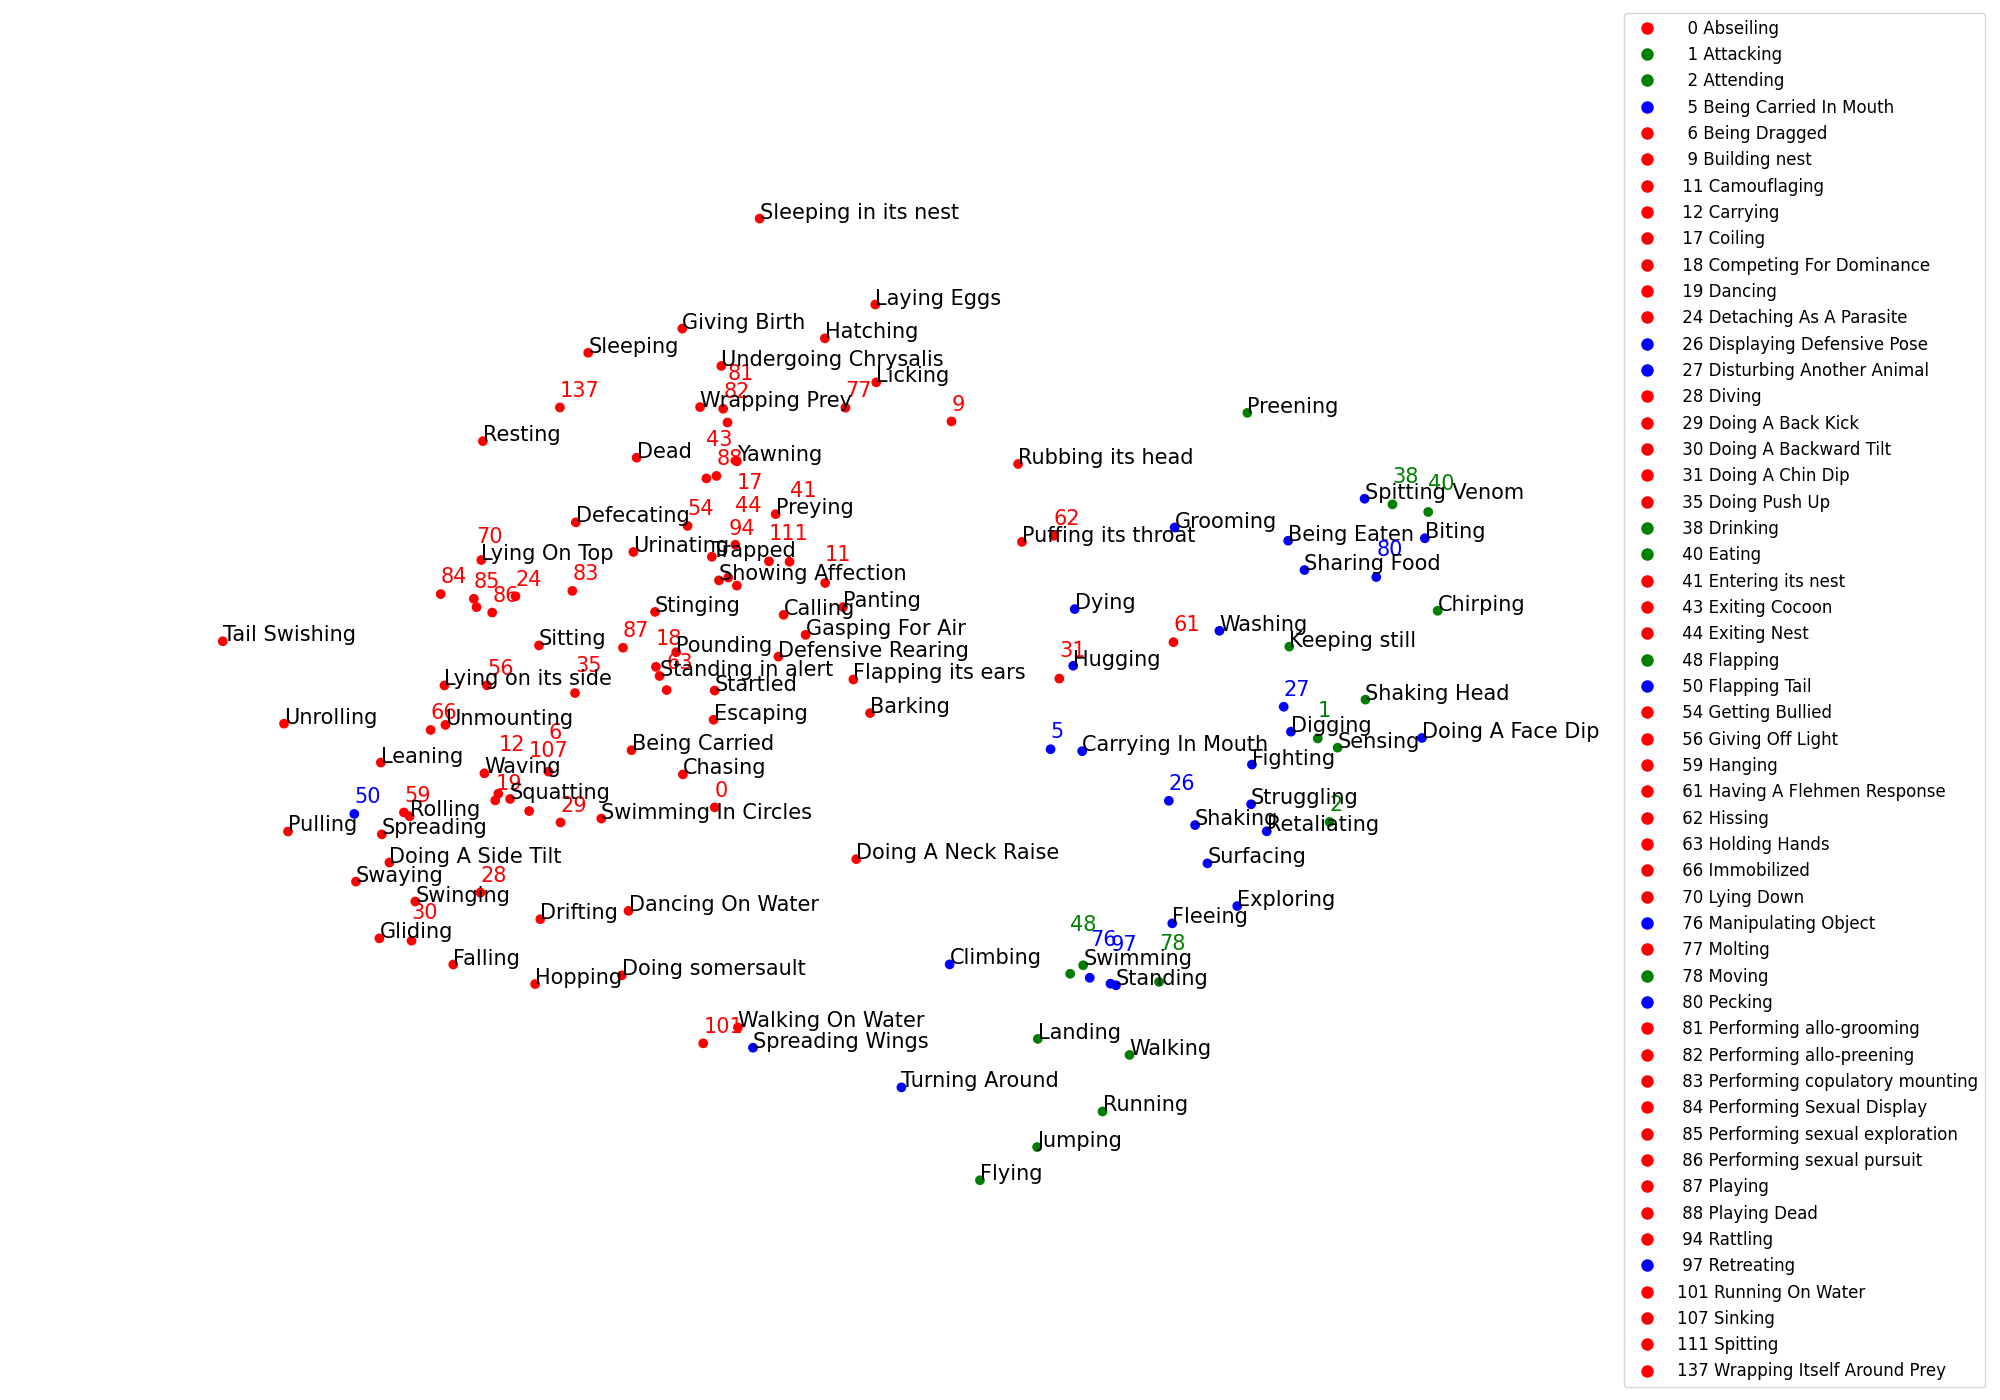
\includegraphics[width=1\textwidth]{assets/imgs/1_1_ClassEmbeddingInternVideo}
    \adjustbox{trim=6.2cm 2cm 5cm 2cm}{%
        \resizebox{1.2\textwidth}{!}{%% Creator: Matplotlib, PGF backend
%%
%% To include the figure in your LaTeX document, write
%%   \input{<filename>.pgf}
%%
%% Make sure the required packages are loaded in your preamble
%%   \usepackage{pgf}
%%
%% Also ensure that all the required font packages are loaded; for instance,
%% the lmodern package is sometimes necessary when using math font.
%%   \usepackage{lmodern}
%%
%% Figures using additional raster images can only be included by \input if
%% they are in the same directory as the main LaTeX file. For loading figures
%% from other directories you can use the `import` package
%%   \usepackage{import}
%%
%% and then include the figures with
%%   \import{<path to file>}{<filename>.pgf}
%%
%% Matplotlib used the following preamble
%%   
%%   \makeatletter\@ifpackageloaded{underscore}{}{\usepackage[strings]{underscore}}\makeatother
%%
\begingroup%
\makeatletter%
\begin{pgfpicture}%
\pgfpathrectangle{\pgfpointorigin}{\pgfqpoint{28.087302in}{22.300000in}}%
\pgfusepath{use as bounding box, clip}%
\begin{pgfscope}%
\pgfsetbuttcap%
\pgfsetmiterjoin%
\definecolor{currentfill}{rgb}{1.000000,1.000000,1.000000}%
\pgfsetfillcolor{currentfill}%
\pgfsetlinewidth{0.000000pt}%
\definecolor{currentstroke}{rgb}{1.000000,1.000000,1.000000}%
\pgfsetstrokecolor{currentstroke}%
\pgfsetdash{}{0pt}%
\pgfpathmoveto{\pgfqpoint{0.000000in}{0.000000in}}%
\pgfpathlineto{\pgfqpoint{28.087302in}{0.000000in}}%
\pgfpathlineto{\pgfqpoint{28.087302in}{22.300000in}}%
\pgfpathlineto{\pgfqpoint{0.000000in}{22.300000in}}%
\pgfpathlineto{\pgfqpoint{0.000000in}{0.000000in}}%
\pgfpathclose%
\pgfusepath{fill}%
\end{pgfscope}%
\begin{pgfscope}%
\pgfsetbuttcap%
\pgfsetmiterjoin%
\definecolor{currentfill}{rgb}{1.000000,1.000000,1.000000}%
\pgfsetfillcolor{currentfill}%
\pgfsetlinewidth{0.000000pt}%
\definecolor{currentstroke}{rgb}{0.000000,0.000000,0.000000}%
\pgfsetstrokecolor{currentstroke}%
\pgfsetstrokeopacity{0.000000}%
\pgfsetdash{}{0pt}%
\pgfpathmoveto{\pgfqpoint{4.300000in}{4.300000in}}%
\pgfpathlineto{\pgfqpoint{23.787302in}{4.300000in}}%
\pgfpathlineto{\pgfqpoint{23.787302in}{18.000000in}}%
\pgfpathlineto{\pgfqpoint{4.300000in}{18.000000in}}%
\pgfpathlineto{\pgfqpoint{4.300000in}{4.300000in}}%
\pgfpathclose%
\pgfusepath{fill}%
\end{pgfscope}%
\begin{pgfscope}%
\pgfpathrectangle{\pgfqpoint{4.300000in}{4.300000in}}{\pgfqpoint{19.487302in}{13.700000in}}%
\pgfusepath{clip}%
\pgfsetbuttcap%
\pgfsetroundjoin%
\definecolor{currentfill}{rgb}{1.000000,0.000000,0.000000}%
\pgfsetfillcolor{currentfill}%
\pgfsetlinewidth{1.003750pt}%
\definecolor{currentstroke}{rgb}{1.000000,0.000000,0.000000}%
\pgfsetstrokecolor{currentstroke}%
\pgfsetdash{}{0pt}%
\pgfpathmoveto{\pgfqpoint{12.819672in}{9.738738in}}%
\pgfpathcurveto{\pgfqpoint{12.830722in}{9.738738in}}{\pgfqpoint{12.841321in}{9.743128in}}{\pgfqpoint{12.849134in}{9.750941in}}%
\pgfpathcurveto{\pgfqpoint{12.856948in}{9.758755in}}{\pgfqpoint{12.861338in}{9.769354in}}{\pgfqpoint{12.861338in}{9.780404in}}%
\pgfpathcurveto{\pgfqpoint{12.861338in}{9.791454in}}{\pgfqpoint{12.856948in}{9.802053in}}{\pgfqpoint{12.849134in}{9.809867in}}%
\pgfpathcurveto{\pgfqpoint{12.841321in}{9.817681in}}{\pgfqpoint{12.830722in}{9.822071in}}{\pgfqpoint{12.819672in}{9.822071in}}%
\pgfpathcurveto{\pgfqpoint{12.808621in}{9.822071in}}{\pgfqpoint{12.798022in}{9.817681in}}{\pgfqpoint{12.790209in}{9.809867in}}%
\pgfpathcurveto{\pgfqpoint{12.782395in}{9.802053in}}{\pgfqpoint{12.778005in}{9.791454in}}{\pgfqpoint{12.778005in}{9.780404in}}%
\pgfpathcurveto{\pgfqpoint{12.778005in}{9.769354in}}{\pgfqpoint{12.782395in}{9.758755in}}{\pgfqpoint{12.790209in}{9.750941in}}%
\pgfpathcurveto{\pgfqpoint{12.798022in}{9.743128in}}{\pgfqpoint{12.808621in}{9.738738in}}{\pgfqpoint{12.819672in}{9.738738in}}%
\pgfpathlineto{\pgfqpoint{12.819672in}{9.738738in}}%
\pgfpathclose%
\pgfusepath{stroke,fill}%
\end{pgfscope}%
\begin{pgfscope}%
\pgfpathrectangle{\pgfqpoint{4.300000in}{4.300000in}}{\pgfqpoint{19.487302in}{13.700000in}}%
\pgfusepath{clip}%
\pgfsetbuttcap%
\pgfsetroundjoin%
\definecolor{currentfill}{rgb}{0.000000,0.501961,0.000000}%
\pgfsetfillcolor{currentfill}%
\pgfsetlinewidth{1.003750pt}%
\definecolor{currentstroke}{rgb}{0.000000,0.501961,0.000000}%
\pgfsetstrokecolor{currentstroke}%
\pgfsetdash{}{0pt}%
\pgfpathmoveto{\pgfqpoint{20.161363in}{10.617819in}}%
\pgfpathcurveto{\pgfqpoint{20.172414in}{10.617819in}}{\pgfqpoint{20.183013in}{10.622209in}}{\pgfqpoint{20.190826in}{10.630023in}}%
\pgfpathcurveto{\pgfqpoint{20.198640in}{10.637836in}}{\pgfqpoint{20.203030in}{10.648435in}}{\pgfqpoint{20.203030in}{10.659486in}}%
\pgfpathcurveto{\pgfqpoint{20.203030in}{10.670536in}}{\pgfqpoint{20.198640in}{10.681135in}}{\pgfqpoint{20.190826in}{10.688948in}}%
\pgfpathcurveto{\pgfqpoint{20.183013in}{10.696762in}}{\pgfqpoint{20.172414in}{10.701152in}}{\pgfqpoint{20.161363in}{10.701152in}}%
\pgfpathcurveto{\pgfqpoint{20.150313in}{10.701152in}}{\pgfqpoint{20.139714in}{10.696762in}}{\pgfqpoint{20.131901in}{10.688948in}}%
\pgfpathcurveto{\pgfqpoint{20.124087in}{10.681135in}}{\pgfqpoint{20.119697in}{10.670536in}}{\pgfqpoint{20.119697in}{10.659486in}}%
\pgfpathcurveto{\pgfqpoint{20.119697in}{10.648435in}}{\pgfqpoint{20.124087in}{10.637836in}}{\pgfqpoint{20.131901in}{10.630023in}}%
\pgfpathcurveto{\pgfqpoint{20.139714in}{10.622209in}}{\pgfqpoint{20.150313in}{10.617819in}}{\pgfqpoint{20.161363in}{10.617819in}}%
\pgfpathlineto{\pgfqpoint{20.161363in}{10.617819in}}%
\pgfpathclose%
\pgfusepath{stroke,fill}%
\end{pgfscope}%
\begin{pgfscope}%
\pgfpathrectangle{\pgfqpoint{4.300000in}{4.300000in}}{\pgfqpoint{19.487302in}{13.700000in}}%
\pgfusepath{clip}%
\pgfsetbuttcap%
\pgfsetroundjoin%
\definecolor{currentfill}{rgb}{0.000000,0.501961,0.000000}%
\pgfsetfillcolor{currentfill}%
\pgfsetlinewidth{1.003750pt}%
\definecolor{currentstroke}{rgb}{0.000000,0.501961,0.000000}%
\pgfsetstrokecolor{currentstroke}%
\pgfsetdash{}{0pt}%
\pgfpathmoveto{\pgfqpoint{20.305694in}{9.551895in}}%
\pgfpathcurveto{\pgfqpoint{20.316744in}{9.551895in}}{\pgfqpoint{20.327343in}{9.556286in}}{\pgfqpoint{20.335157in}{9.564099in}}%
\pgfpathcurveto{\pgfqpoint{20.342970in}{9.571913in}}{\pgfqpoint{20.347361in}{9.582512in}}{\pgfqpoint{20.347361in}{9.593562in}}%
\pgfpathcurveto{\pgfqpoint{20.347361in}{9.604612in}}{\pgfqpoint{20.342970in}{9.615211in}}{\pgfqpoint{20.335157in}{9.623025in}}%
\pgfpathcurveto{\pgfqpoint{20.327343in}{9.630838in}}{\pgfqpoint{20.316744in}{9.635229in}}{\pgfqpoint{20.305694in}{9.635229in}}%
\pgfpathcurveto{\pgfqpoint{20.294644in}{9.635229in}}{\pgfqpoint{20.284045in}{9.630838in}}{\pgfqpoint{20.276231in}{9.623025in}}%
\pgfpathcurveto{\pgfqpoint{20.268417in}{9.615211in}}{\pgfqpoint{20.264027in}{9.604612in}}{\pgfqpoint{20.264027in}{9.593562in}}%
\pgfpathcurveto{\pgfqpoint{20.264027in}{9.582512in}}{\pgfqpoint{20.268417in}{9.571913in}}{\pgfqpoint{20.276231in}{9.564099in}}%
\pgfpathcurveto{\pgfqpoint{20.284045in}{9.556286in}}{\pgfqpoint{20.294644in}{9.551895in}}{\pgfqpoint{20.305694in}{9.551895in}}%
\pgfpathlineto{\pgfqpoint{20.305694in}{9.551895in}}%
\pgfpathclose%
\pgfusepath{stroke,fill}%
\end{pgfscope}%
\begin{pgfscope}%
\pgfpathrectangle{\pgfqpoint{4.300000in}{4.300000in}}{\pgfqpoint{19.487302in}{13.700000in}}%
\pgfusepath{clip}%
\pgfsetbuttcap%
\pgfsetroundjoin%
\definecolor{currentfill}{rgb}{1.000000,0.000000,0.000000}%
\pgfsetfillcolor{currentfill}%
\pgfsetlinewidth{1.003750pt}%
\definecolor{currentstroke}{rgb}{1.000000,0.000000,0.000000}%
\pgfsetstrokecolor{currentstroke}%
\pgfsetdash{}{0pt}%
\pgfpathmoveto{\pgfqpoint{14.710709in}{10.941280in}}%
\pgfpathcurveto{\pgfqpoint{14.721759in}{10.941280in}}{\pgfqpoint{14.732358in}{10.945671in}}{\pgfqpoint{14.740172in}{10.953484in}}%
\pgfpathcurveto{\pgfqpoint{14.747986in}{10.961298in}}{\pgfqpoint{14.752376in}{10.971897in}}{\pgfqpoint{14.752376in}{10.982947in}}%
\pgfpathcurveto{\pgfqpoint{14.752376in}{10.993997in}}{\pgfqpoint{14.747986in}{11.004596in}}{\pgfqpoint{14.740172in}{11.012410in}}%
\pgfpathcurveto{\pgfqpoint{14.732358in}{11.020223in}}{\pgfqpoint{14.721759in}{11.024614in}}{\pgfqpoint{14.710709in}{11.024614in}}%
\pgfpathcurveto{\pgfqpoint{14.699659in}{11.024614in}}{\pgfqpoint{14.689060in}{11.020223in}}{\pgfqpoint{14.681246in}{11.012410in}}%
\pgfpathcurveto{\pgfqpoint{14.673433in}{11.004596in}}{\pgfqpoint{14.669043in}{10.993997in}}{\pgfqpoint{14.669043in}{10.982947in}}%
\pgfpathcurveto{\pgfqpoint{14.669043in}{10.971897in}}{\pgfqpoint{14.673433in}{10.961298in}}{\pgfqpoint{14.681246in}{10.953484in}}%
\pgfpathcurveto{\pgfqpoint{14.689060in}{10.945671in}}{\pgfqpoint{14.699659in}{10.941280in}}{\pgfqpoint{14.710709in}{10.941280in}}%
\pgfpathlineto{\pgfqpoint{14.710709in}{10.941280in}}%
\pgfpathclose%
\pgfusepath{stroke,fill}%
\end{pgfscope}%
\begin{pgfscope}%
\pgfpathrectangle{\pgfqpoint{4.300000in}{4.300000in}}{\pgfqpoint{19.487302in}{13.700000in}}%
\pgfusepath{clip}%
\pgfsetbuttcap%
\pgfsetroundjoin%
\definecolor{currentfill}{rgb}{1.000000,0.000000,0.000000}%
\pgfsetfillcolor{currentfill}%
\pgfsetlinewidth{1.003750pt}%
\definecolor{currentstroke}{rgb}{1.000000,0.000000,0.000000}%
\pgfsetstrokecolor{currentstroke}%
\pgfsetdash{}{0pt}%
\pgfpathmoveto{\pgfqpoint{11.806375in}{10.468083in}}%
\pgfpathcurveto{\pgfqpoint{11.817425in}{10.468083in}}{\pgfqpoint{11.828024in}{10.472473in}}{\pgfqpoint{11.835838in}{10.480287in}}%
\pgfpathcurveto{\pgfqpoint{11.843651in}{10.488101in}}{\pgfqpoint{11.848042in}{10.498700in}}{\pgfqpoint{11.848042in}{10.509750in}}%
\pgfpathcurveto{\pgfqpoint{11.848042in}{10.520800in}}{\pgfqpoint{11.843651in}{10.531399in}}{\pgfqpoint{11.835838in}{10.539212in}}%
\pgfpathcurveto{\pgfqpoint{11.828024in}{10.547026in}}{\pgfqpoint{11.817425in}{10.551416in}}{\pgfqpoint{11.806375in}{10.551416in}}%
\pgfpathcurveto{\pgfqpoint{11.795325in}{10.551416in}}{\pgfqpoint{11.784726in}{10.547026in}}{\pgfqpoint{11.776912in}{10.539212in}}%
\pgfpathcurveto{\pgfqpoint{11.769099in}{10.531399in}}{\pgfqpoint{11.764708in}{10.520800in}}{\pgfqpoint{11.764708in}{10.509750in}}%
\pgfpathcurveto{\pgfqpoint{11.764708in}{10.498700in}}{\pgfqpoint{11.769099in}{10.488101in}}{\pgfqpoint{11.776912in}{10.480287in}}%
\pgfpathcurveto{\pgfqpoint{11.784726in}{10.472473in}}{\pgfqpoint{11.795325in}{10.468083in}}{\pgfqpoint{11.806375in}{10.468083in}}%
\pgfpathlineto{\pgfqpoint{11.806375in}{10.468083in}}%
\pgfpathclose%
\pgfusepath{stroke,fill}%
\end{pgfscope}%
\begin{pgfscope}%
\pgfpathrectangle{\pgfqpoint{4.300000in}{4.300000in}}{\pgfqpoint{19.487302in}{13.700000in}}%
\pgfusepath{clip}%
\pgfsetbuttcap%
\pgfsetroundjoin%
\definecolor{currentfill}{rgb}{0.000000,0.000000,1.000000}%
\pgfsetfillcolor{currentfill}%
\pgfsetlinewidth{1.003750pt}%
\definecolor{currentstroke}{rgb}{0.000000,0.000000,1.000000}%
\pgfsetstrokecolor{currentstroke}%
\pgfsetdash{}{0pt}%
\pgfpathmoveto{\pgfqpoint{16.908504in}{10.480295in}}%
\pgfpathcurveto{\pgfqpoint{16.919554in}{10.480295in}}{\pgfqpoint{16.930153in}{10.484685in}}{\pgfqpoint{16.937967in}{10.492499in}}%
\pgfpathcurveto{\pgfqpoint{16.945781in}{10.500313in}}{\pgfqpoint{16.950171in}{10.510912in}}{\pgfqpoint{16.950171in}{10.521962in}}%
\pgfpathcurveto{\pgfqpoint{16.950171in}{10.533012in}}{\pgfqpoint{16.945781in}{10.543611in}}{\pgfqpoint{16.937967in}{10.551425in}}%
\pgfpathcurveto{\pgfqpoint{16.930153in}{10.559238in}}{\pgfqpoint{16.919554in}{10.563628in}}{\pgfqpoint{16.908504in}{10.563628in}}%
\pgfpathcurveto{\pgfqpoint{16.897454in}{10.563628in}}{\pgfqpoint{16.886855in}{10.559238in}}{\pgfqpoint{16.879041in}{10.551425in}}%
\pgfpathcurveto{\pgfqpoint{16.871228in}{10.543611in}}{\pgfqpoint{16.866838in}{10.533012in}}{\pgfqpoint{16.866838in}{10.521962in}}%
\pgfpathcurveto{\pgfqpoint{16.866838in}{10.510912in}}{\pgfqpoint{16.871228in}{10.500313in}}{\pgfqpoint{16.879041in}{10.492499in}}%
\pgfpathcurveto{\pgfqpoint{16.886855in}{10.484685in}}{\pgfqpoint{16.897454in}{10.480295in}}{\pgfqpoint{16.908504in}{10.480295in}}%
\pgfpathlineto{\pgfqpoint{16.908504in}{10.480295in}}%
\pgfpathclose%
\pgfusepath{stroke,fill}%
\end{pgfscope}%
\begin{pgfscope}%
\pgfpathrectangle{\pgfqpoint{4.300000in}{4.300000in}}{\pgfqpoint{19.487302in}{13.700000in}}%
\pgfusepath{clip}%
\pgfsetbuttcap%
\pgfsetroundjoin%
\definecolor{currentfill}{rgb}{1.000000,0.000000,0.000000}%
\pgfsetfillcolor{currentfill}%
\pgfsetlinewidth{1.003750pt}%
\definecolor{currentstroke}{rgb}{1.000000,0.000000,0.000000}%
\pgfsetstrokecolor{currentstroke}%
\pgfsetdash{}{0pt}%
\pgfpathmoveto{\pgfqpoint{10.795488in}{10.194071in}}%
\pgfpathcurveto{\pgfqpoint{10.806538in}{10.194071in}}{\pgfqpoint{10.817137in}{10.198462in}}{\pgfqpoint{10.824951in}{10.206275in}}%
\pgfpathcurveto{\pgfqpoint{10.832765in}{10.214089in}}{\pgfqpoint{10.837155in}{10.224688in}}{\pgfqpoint{10.837155in}{10.235738in}}%
\pgfpathcurveto{\pgfqpoint{10.837155in}{10.246788in}}{\pgfqpoint{10.832765in}{10.257387in}}{\pgfqpoint{10.824951in}{10.265201in}}%
\pgfpathcurveto{\pgfqpoint{10.817137in}{10.273015in}}{\pgfqpoint{10.806538in}{10.277405in}}{\pgfqpoint{10.795488in}{10.277405in}}%
\pgfpathcurveto{\pgfqpoint{10.784438in}{10.277405in}}{\pgfqpoint{10.773839in}{10.273015in}}{\pgfqpoint{10.766026in}{10.265201in}}%
\pgfpathcurveto{\pgfqpoint{10.758212in}{10.257387in}}{\pgfqpoint{10.753822in}{10.246788in}}{\pgfqpoint{10.753822in}{10.235738in}}%
\pgfpathcurveto{\pgfqpoint{10.753822in}{10.224688in}}{\pgfqpoint{10.758212in}{10.214089in}}{\pgfqpoint{10.766026in}{10.206275in}}%
\pgfpathcurveto{\pgfqpoint{10.773839in}{10.198462in}}{\pgfqpoint{10.784438in}{10.194071in}}{\pgfqpoint{10.795488in}{10.194071in}}%
\pgfpathlineto{\pgfqpoint{10.795488in}{10.194071in}}%
\pgfpathclose%
\pgfusepath{stroke,fill}%
\end{pgfscope}%
\begin{pgfscope}%
\pgfpathrectangle{\pgfqpoint{4.300000in}{4.300000in}}{\pgfqpoint{19.487302in}{13.700000in}}%
\pgfusepath{clip}%
\pgfsetbuttcap%
\pgfsetroundjoin%
\definecolor{currentfill}{rgb}{0.000000,0.000000,1.000000}%
\pgfsetfillcolor{currentfill}%
\pgfsetlinewidth{1.003750pt}%
\definecolor{currentstroke}{rgb}{0.000000,0.000000,1.000000}%
\pgfsetstrokecolor{currentstroke}%
\pgfsetdash{}{0pt}%
\pgfpathmoveto{\pgfqpoint{19.801535in}{13.140961in}}%
\pgfpathcurveto{\pgfqpoint{19.812586in}{13.140961in}}{\pgfqpoint{19.823185in}{13.145351in}}{\pgfqpoint{19.830998in}{13.153165in}}%
\pgfpathcurveto{\pgfqpoint{19.838812in}{13.160978in}}{\pgfqpoint{19.843202in}{13.171577in}}{\pgfqpoint{19.843202in}{13.182628in}}%
\pgfpathcurveto{\pgfqpoint{19.843202in}{13.193678in}}{\pgfqpoint{19.838812in}{13.204277in}}{\pgfqpoint{19.830998in}{13.212090in}}%
\pgfpathcurveto{\pgfqpoint{19.823185in}{13.219904in}}{\pgfqpoint{19.812586in}{13.224294in}}{\pgfqpoint{19.801535in}{13.224294in}}%
\pgfpathcurveto{\pgfqpoint{19.790485in}{13.224294in}}{\pgfqpoint{19.779886in}{13.219904in}}{\pgfqpoint{19.772073in}{13.212090in}}%
\pgfpathcurveto{\pgfqpoint{19.764259in}{13.204277in}}{\pgfqpoint{19.759869in}{13.193678in}}{\pgfqpoint{19.759869in}{13.182628in}}%
\pgfpathcurveto{\pgfqpoint{19.759869in}{13.171577in}}{\pgfqpoint{19.764259in}{13.160978in}}{\pgfqpoint{19.772073in}{13.153165in}}%
\pgfpathcurveto{\pgfqpoint{19.779886in}{13.145351in}}{\pgfqpoint{19.790485in}{13.140961in}}{\pgfqpoint{19.801535in}{13.140961in}}%
\pgfpathlineto{\pgfqpoint{19.801535in}{13.140961in}}%
\pgfpathclose%
\pgfusepath{stroke,fill}%
\end{pgfscope}%
\begin{pgfscope}%
\pgfpathrectangle{\pgfqpoint{4.300000in}{4.300000in}}{\pgfqpoint{19.487302in}{13.700000in}}%
\pgfusepath{clip}%
\pgfsetbuttcap%
\pgfsetroundjoin%
\definecolor{currentfill}{rgb}{0.000000,0.000000,1.000000}%
\pgfsetfillcolor{currentfill}%
\pgfsetlinewidth{1.003750pt}%
\definecolor{currentstroke}{rgb}{0.000000,0.000000,1.000000}%
\pgfsetstrokecolor{currentstroke}%
\pgfsetdash{}{0pt}%
\pgfpathmoveto{\pgfqpoint{21.465899in}{13.172032in}}%
\pgfpathcurveto{\pgfqpoint{21.476950in}{13.172032in}}{\pgfqpoint{21.487549in}{13.176422in}}{\pgfqpoint{21.495362in}{13.184236in}}%
\pgfpathcurveto{\pgfqpoint{21.503176in}{13.192049in}}{\pgfqpoint{21.507566in}{13.202648in}}{\pgfqpoint{21.507566in}{13.213698in}}%
\pgfpathcurveto{\pgfqpoint{21.507566in}{13.224748in}}{\pgfqpoint{21.503176in}{13.235347in}}{\pgfqpoint{21.495362in}{13.243161in}}%
\pgfpathcurveto{\pgfqpoint{21.487549in}{13.250975in}}{\pgfqpoint{21.476950in}{13.255365in}}{\pgfqpoint{21.465899in}{13.255365in}}%
\pgfpathcurveto{\pgfqpoint{21.454849in}{13.255365in}}{\pgfqpoint{21.444250in}{13.250975in}}{\pgfqpoint{21.436437in}{13.243161in}}%
\pgfpathcurveto{\pgfqpoint{21.428623in}{13.235347in}}{\pgfqpoint{21.424233in}{13.224748in}}{\pgfqpoint{21.424233in}{13.213698in}}%
\pgfpathcurveto{\pgfqpoint{21.424233in}{13.202648in}}{\pgfqpoint{21.428623in}{13.192049in}}{\pgfqpoint{21.436437in}{13.184236in}}%
\pgfpathcurveto{\pgfqpoint{21.444250in}{13.176422in}}{\pgfqpoint{21.454849in}{13.172032in}}{\pgfqpoint{21.465899in}{13.172032in}}%
\pgfpathlineto{\pgfqpoint{21.465899in}{13.172032in}}%
\pgfpathclose%
\pgfusepath{stroke,fill}%
\end{pgfscope}%
\begin{pgfscope}%
\pgfpathrectangle{\pgfqpoint{4.300000in}{4.300000in}}{\pgfqpoint{19.487302in}{13.700000in}}%
\pgfusepath{clip}%
\pgfsetbuttcap%
\pgfsetroundjoin%
\definecolor{currentfill}{rgb}{1.000000,0.000000,0.000000}%
\pgfsetfillcolor{currentfill}%
\pgfsetlinewidth{1.003750pt}%
\definecolor{currentstroke}{rgb}{1.000000,0.000000,0.000000}%
\pgfsetstrokecolor{currentstroke}%
\pgfsetdash{}{0pt}%
\pgfpathmoveto{\pgfqpoint{15.701838in}{14.663091in}}%
\pgfpathcurveto{\pgfqpoint{15.712888in}{14.663091in}}{\pgfqpoint{15.723487in}{14.667481in}}{\pgfqpoint{15.731300in}{14.675295in}}%
\pgfpathcurveto{\pgfqpoint{15.739114in}{14.683108in}}{\pgfqpoint{15.743504in}{14.693707in}}{\pgfqpoint{15.743504in}{14.704758in}}%
\pgfpathcurveto{\pgfqpoint{15.743504in}{14.715808in}}{\pgfqpoint{15.739114in}{14.726407in}}{\pgfqpoint{15.731300in}{14.734220in}}%
\pgfpathcurveto{\pgfqpoint{15.723487in}{14.742034in}}{\pgfqpoint{15.712888in}{14.746424in}}{\pgfqpoint{15.701838in}{14.746424in}}%
\pgfpathcurveto{\pgfqpoint{15.690787in}{14.746424in}}{\pgfqpoint{15.680188in}{14.742034in}}{\pgfqpoint{15.672375in}{14.734220in}}%
\pgfpathcurveto{\pgfqpoint{15.664561in}{14.726407in}}{\pgfqpoint{15.660171in}{14.715808in}}{\pgfqpoint{15.660171in}{14.704758in}}%
\pgfpathcurveto{\pgfqpoint{15.660171in}{14.693707in}}{\pgfqpoint{15.664561in}{14.683108in}}{\pgfqpoint{15.672375in}{14.675295in}}%
\pgfpathcurveto{\pgfqpoint{15.680188in}{14.667481in}}{\pgfqpoint{15.690787in}{14.663091in}}{\pgfqpoint{15.701838in}{14.663091in}}%
\pgfpathlineto{\pgfqpoint{15.701838in}{14.663091in}}%
\pgfpathclose%
\pgfusepath{stroke,fill}%
\end{pgfscope}%
\begin{pgfscope}%
\pgfpathrectangle{\pgfqpoint{4.300000in}{4.300000in}}{\pgfqpoint{19.487302in}{13.700000in}}%
\pgfusepath{clip}%
\pgfsetbuttcap%
\pgfsetroundjoin%
\definecolor{currentfill}{rgb}{1.000000,0.000000,0.000000}%
\pgfsetfillcolor{currentfill}%
\pgfsetlinewidth{1.003750pt}%
\definecolor{currentstroke}{rgb}{1.000000,0.000000,0.000000}%
\pgfsetstrokecolor{currentstroke}%
\pgfsetdash{}{0pt}%
\pgfpathmoveto{\pgfqpoint{13.658466in}{12.194681in}}%
\pgfpathcurveto{\pgfqpoint{13.669517in}{12.194681in}}{\pgfqpoint{13.680116in}{12.199071in}}{\pgfqpoint{13.687929in}{12.206885in}}%
\pgfpathcurveto{\pgfqpoint{13.695743in}{12.214698in}}{\pgfqpoint{13.700133in}{12.225297in}}{\pgfqpoint{13.700133in}{12.236348in}}%
\pgfpathcurveto{\pgfqpoint{13.700133in}{12.247398in}}{\pgfqpoint{13.695743in}{12.257997in}}{\pgfqpoint{13.687929in}{12.265810in}}%
\pgfpathcurveto{\pgfqpoint{13.680116in}{12.273624in}}{\pgfqpoint{13.669517in}{12.278014in}}{\pgfqpoint{13.658466in}{12.278014in}}%
\pgfpathcurveto{\pgfqpoint{13.647416in}{12.278014in}}{\pgfqpoint{13.636817in}{12.273624in}}{\pgfqpoint{13.629004in}{12.265810in}}%
\pgfpathcurveto{\pgfqpoint{13.621190in}{12.257997in}}{\pgfqpoint{13.616800in}{12.247398in}}{\pgfqpoint{13.616800in}{12.236348in}}%
\pgfpathcurveto{\pgfqpoint{13.616800in}{12.225297in}}{\pgfqpoint{13.621190in}{12.214698in}}{\pgfqpoint{13.629004in}{12.206885in}}%
\pgfpathcurveto{\pgfqpoint{13.636817in}{12.199071in}}{\pgfqpoint{13.647416in}{12.194681in}}{\pgfqpoint{13.658466in}{12.194681in}}%
\pgfpathlineto{\pgfqpoint{13.658466in}{12.194681in}}%
\pgfpathclose%
\pgfusepath{stroke,fill}%
\end{pgfscope}%
\begin{pgfscope}%
\pgfpathrectangle{\pgfqpoint{4.300000in}{4.300000in}}{\pgfqpoint{19.487302in}{13.700000in}}%
\pgfusepath{clip}%
\pgfsetbuttcap%
\pgfsetroundjoin%
\definecolor{currentfill}{rgb}{1.000000,0.000000,0.000000}%
\pgfsetfillcolor{currentfill}%
\pgfsetlinewidth{1.003750pt}%
\definecolor{currentstroke}{rgb}{1.000000,0.000000,0.000000}%
\pgfsetstrokecolor{currentstroke}%
\pgfsetdash{}{0pt}%
\pgfpathmoveto{\pgfqpoint{14.164245in}{12.601756in}}%
\pgfpathcurveto{\pgfqpoint{14.175295in}{12.601756in}}{\pgfqpoint{14.185894in}{12.606146in}}{\pgfqpoint{14.193707in}{12.613959in}}%
\pgfpathcurveto{\pgfqpoint{14.201521in}{12.621773in}}{\pgfqpoint{14.205911in}{12.632372in}}{\pgfqpoint{14.205911in}{12.643422in}}%
\pgfpathcurveto{\pgfqpoint{14.205911in}{12.654472in}}{\pgfqpoint{14.201521in}{12.665071in}}{\pgfqpoint{14.193707in}{12.672885in}}%
\pgfpathcurveto{\pgfqpoint{14.185894in}{12.680699in}}{\pgfqpoint{14.175295in}{12.685089in}}{\pgfqpoint{14.164245in}{12.685089in}}%
\pgfpathcurveto{\pgfqpoint{14.153194in}{12.685089in}}{\pgfqpoint{14.142595in}{12.680699in}}{\pgfqpoint{14.134782in}{12.672885in}}%
\pgfpathcurveto{\pgfqpoint{14.126968in}{12.665071in}}{\pgfqpoint{14.122578in}{12.654472in}}{\pgfqpoint{14.122578in}{12.643422in}}%
\pgfpathcurveto{\pgfqpoint{14.122578in}{12.632372in}}{\pgfqpoint{14.126968in}{12.621773in}}{\pgfqpoint{14.134782in}{12.613959in}}%
\pgfpathcurveto{\pgfqpoint{14.142595in}{12.606146in}}{\pgfqpoint{14.153194in}{12.601756in}}{\pgfqpoint{14.164245in}{12.601756in}}%
\pgfpathlineto{\pgfqpoint{14.164245in}{12.601756in}}%
\pgfpathclose%
\pgfusepath{stroke,fill}%
\end{pgfscope}%
\begin{pgfscope}%
\pgfpathrectangle{\pgfqpoint{4.300000in}{4.300000in}}{\pgfqpoint{19.487302in}{13.700000in}}%
\pgfusepath{clip}%
\pgfsetbuttcap%
\pgfsetroundjoin%
\definecolor{currentfill}{rgb}{1.000000,0.000000,0.000000}%
\pgfsetfillcolor{currentfill}%
\pgfsetlinewidth{1.003750pt}%
\definecolor{currentstroke}{rgb}{1.000000,0.000000,0.000000}%
\pgfsetstrokecolor{currentstroke}%
\pgfsetdash{}{0pt}%
\pgfpathmoveto{\pgfqpoint{10.184486in}{9.912011in}}%
\pgfpathcurveto{\pgfqpoint{10.195536in}{9.912011in}}{\pgfqpoint{10.206135in}{9.916401in}}{\pgfqpoint{10.213949in}{9.924215in}}%
\pgfpathcurveto{\pgfqpoint{10.221763in}{9.932029in}}{\pgfqpoint{10.226153in}{9.942628in}}{\pgfqpoint{10.226153in}{9.953678in}}%
\pgfpathcurveto{\pgfqpoint{10.226153in}{9.964728in}}{\pgfqpoint{10.221763in}{9.975327in}}{\pgfqpoint{10.213949in}{9.983141in}}%
\pgfpathcurveto{\pgfqpoint{10.206135in}{9.990954in}}{\pgfqpoint{10.195536in}{9.995344in}}{\pgfqpoint{10.184486in}{9.995344in}}%
\pgfpathcurveto{\pgfqpoint{10.173436in}{9.995344in}}{\pgfqpoint{10.162837in}{9.990954in}}{\pgfqpoint{10.155023in}{9.983141in}}%
\pgfpathcurveto{\pgfqpoint{10.147210in}{9.975327in}}{\pgfqpoint{10.142819in}{9.964728in}}{\pgfqpoint{10.142819in}{9.953678in}}%
\pgfpathcurveto{\pgfqpoint{10.142819in}{9.942628in}}{\pgfqpoint{10.147210in}{9.932029in}}{\pgfqpoint{10.155023in}{9.924215in}}%
\pgfpathcurveto{\pgfqpoint{10.162837in}{9.916401in}}{\pgfqpoint{10.173436in}{9.912011in}}{\pgfqpoint{10.184486in}{9.912011in}}%
\pgfpathlineto{\pgfqpoint{10.184486in}{9.912011in}}%
\pgfpathclose%
\pgfusepath{stroke,fill}%
\end{pgfscope}%
\begin{pgfscope}%
\pgfpathrectangle{\pgfqpoint{4.300000in}{4.300000in}}{\pgfqpoint{19.487302in}{13.700000in}}%
\pgfusepath{clip}%
\pgfsetbuttcap%
\pgfsetroundjoin%
\definecolor{currentfill}{rgb}{0.000000,0.000000,1.000000}%
\pgfsetfillcolor{currentfill}%
\pgfsetlinewidth{1.003750pt}%
\definecolor{currentstroke}{rgb}{0.000000,0.000000,1.000000}%
\pgfsetstrokecolor{currentstroke}%
\pgfsetdash{}{0pt}%
\pgfpathmoveto{\pgfqpoint{17.293231in}{10.455485in}}%
\pgfpathcurveto{\pgfqpoint{17.304281in}{10.455485in}}{\pgfqpoint{17.314880in}{10.459876in}}{\pgfqpoint{17.322693in}{10.467689in}}%
\pgfpathcurveto{\pgfqpoint{17.330507in}{10.475503in}}{\pgfqpoint{17.334897in}{10.486102in}}{\pgfqpoint{17.334897in}{10.497152in}}%
\pgfpathcurveto{\pgfqpoint{17.334897in}{10.508202in}}{\pgfqpoint{17.330507in}{10.518801in}}{\pgfqpoint{17.322693in}{10.526615in}}%
\pgfpathcurveto{\pgfqpoint{17.314880in}{10.534428in}}{\pgfqpoint{17.304281in}{10.538819in}}{\pgfqpoint{17.293231in}{10.538819in}}%
\pgfpathcurveto{\pgfqpoint{17.282180in}{10.538819in}}{\pgfqpoint{17.271581in}{10.534428in}}{\pgfqpoint{17.263768in}{10.526615in}}%
\pgfpathcurveto{\pgfqpoint{17.255954in}{10.518801in}}{\pgfqpoint{17.251564in}{10.508202in}}{\pgfqpoint{17.251564in}{10.497152in}}%
\pgfpathcurveto{\pgfqpoint{17.251564in}{10.486102in}}{\pgfqpoint{17.255954in}{10.475503in}}{\pgfqpoint{17.263768in}{10.467689in}}%
\pgfpathcurveto{\pgfqpoint{17.271581in}{10.459876in}}{\pgfqpoint{17.282180in}{10.455485in}}{\pgfqpoint{17.293231in}{10.455485in}}%
\pgfpathlineto{\pgfqpoint{17.293231in}{10.455485in}}%
\pgfpathclose%
\pgfusepath{stroke,fill}%
\end{pgfscope}%
\begin{pgfscope}%
\pgfpathrectangle{\pgfqpoint{4.300000in}{4.300000in}}{\pgfqpoint{19.487302in}{13.700000in}}%
\pgfusepath{clip}%
\pgfsetbuttcap%
\pgfsetroundjoin%
\definecolor{currentfill}{rgb}{1.000000,0.000000,0.000000}%
\pgfsetfillcolor{currentfill}%
\pgfsetlinewidth{1.003750pt}%
\definecolor{currentstroke}{rgb}{1.000000,0.000000,0.000000}%
\pgfsetstrokecolor{currentstroke}%
\pgfsetdash{}{0pt}%
\pgfpathmoveto{\pgfqpoint{12.432214in}{10.158871in}}%
\pgfpathcurveto{\pgfqpoint{12.443264in}{10.158871in}}{\pgfqpoint{12.453863in}{10.163261in}}{\pgfqpoint{12.461677in}{10.171075in}}%
\pgfpathcurveto{\pgfqpoint{12.469491in}{10.178888in}}{\pgfqpoint{12.473881in}{10.189487in}}{\pgfqpoint{12.473881in}{10.200537in}}%
\pgfpathcurveto{\pgfqpoint{12.473881in}{10.211588in}}{\pgfqpoint{12.469491in}{10.222187in}}{\pgfqpoint{12.461677in}{10.230000in}}%
\pgfpathcurveto{\pgfqpoint{12.453863in}{10.237814in}}{\pgfqpoint{12.443264in}{10.242204in}}{\pgfqpoint{12.432214in}{10.242204in}}%
\pgfpathcurveto{\pgfqpoint{12.421164in}{10.242204in}}{\pgfqpoint{12.410565in}{10.237814in}}{\pgfqpoint{12.402751in}{10.230000in}}%
\pgfpathcurveto{\pgfqpoint{12.394938in}{10.222187in}}{\pgfqpoint{12.390548in}{10.211588in}}{\pgfqpoint{12.390548in}{10.200537in}}%
\pgfpathcurveto{\pgfqpoint{12.390548in}{10.189487in}}{\pgfqpoint{12.394938in}{10.178888in}}{\pgfqpoint{12.402751in}{10.171075in}}%
\pgfpathcurveto{\pgfqpoint{12.410565in}{10.163261in}}{\pgfqpoint{12.421164in}{10.158871in}}{\pgfqpoint{12.432214in}{10.158871in}}%
\pgfpathlineto{\pgfqpoint{12.432214in}{10.158871in}}%
\pgfpathclose%
\pgfusepath{stroke,fill}%
\end{pgfscope}%
\begin{pgfscope}%
\pgfpathrectangle{\pgfqpoint{4.300000in}{4.300000in}}{\pgfqpoint{19.487302in}{13.700000in}}%
\pgfusepath{clip}%
\pgfsetbuttcap%
\pgfsetroundjoin%
\definecolor{currentfill}{rgb}{0.000000,0.501961,0.000000}%
\pgfsetfillcolor{currentfill}%
\pgfsetlinewidth{1.003750pt}%
\definecolor{currentstroke}{rgb}{0.000000,0.501961,0.000000}%
\pgfsetstrokecolor{currentstroke}%
\pgfsetdash{}{0pt}%
\pgfpathmoveto{\pgfqpoint{21.621280in}{12.246540in}}%
\pgfpathcurveto{\pgfqpoint{21.632330in}{12.246540in}}{\pgfqpoint{21.642929in}{12.250930in}}{\pgfqpoint{21.650742in}{12.258744in}}%
\pgfpathcurveto{\pgfqpoint{21.658556in}{12.266557in}}{\pgfqpoint{21.662946in}{12.277156in}}{\pgfqpoint{21.662946in}{12.288206in}}%
\pgfpathcurveto{\pgfqpoint{21.662946in}{12.299257in}}{\pgfqpoint{21.658556in}{12.309856in}}{\pgfqpoint{21.650742in}{12.317669in}}%
\pgfpathcurveto{\pgfqpoint{21.642929in}{12.325483in}}{\pgfqpoint{21.632330in}{12.329873in}}{\pgfqpoint{21.621280in}{12.329873in}}%
\pgfpathcurveto{\pgfqpoint{21.610229in}{12.329873in}}{\pgfqpoint{21.599630in}{12.325483in}}{\pgfqpoint{21.591817in}{12.317669in}}%
\pgfpathcurveto{\pgfqpoint{21.584003in}{12.309856in}}{\pgfqpoint{21.579613in}{12.299257in}}{\pgfqpoint{21.579613in}{12.288206in}}%
\pgfpathcurveto{\pgfqpoint{21.579613in}{12.277156in}}{\pgfqpoint{21.584003in}{12.266557in}}{\pgfqpoint{21.591817in}{12.258744in}}%
\pgfpathcurveto{\pgfqpoint{21.599630in}{12.250930in}}{\pgfqpoint{21.610229in}{12.246540in}}{\pgfqpoint{21.621280in}{12.246540in}}%
\pgfpathlineto{\pgfqpoint{21.621280in}{12.246540in}}%
\pgfpathclose%
\pgfusepath{stroke,fill}%
\end{pgfscope}%
\begin{pgfscope}%
\pgfpathrectangle{\pgfqpoint{4.300000in}{4.300000in}}{\pgfqpoint{19.487302in}{13.700000in}}%
\pgfusepath{clip}%
\pgfsetbuttcap%
\pgfsetroundjoin%
\definecolor{currentfill}{rgb}{0.000000,0.000000,1.000000}%
\pgfsetfillcolor{currentfill}%
\pgfsetlinewidth{1.003750pt}%
\definecolor{currentstroke}{rgb}{0.000000,0.000000,1.000000}%
\pgfsetstrokecolor{currentstroke}%
\pgfsetdash{}{0pt}%
\pgfpathmoveto{\pgfqpoint{15.679626in}{7.734639in}}%
\pgfpathcurveto{\pgfqpoint{15.690676in}{7.734639in}}{\pgfqpoint{15.701275in}{7.739029in}}{\pgfqpoint{15.709089in}{7.746843in}}%
\pgfpathcurveto{\pgfqpoint{15.716902in}{7.754656in}}{\pgfqpoint{15.721293in}{7.765255in}}{\pgfqpoint{15.721293in}{7.776305in}}%
\pgfpathcurveto{\pgfqpoint{15.721293in}{7.787355in}}{\pgfqpoint{15.716902in}{7.797954in}}{\pgfqpoint{15.709089in}{7.805768in}}%
\pgfpathcurveto{\pgfqpoint{15.701275in}{7.813582in}}{\pgfqpoint{15.690676in}{7.817972in}}{\pgfqpoint{15.679626in}{7.817972in}}%
\pgfpathcurveto{\pgfqpoint{15.668576in}{7.817972in}}{\pgfqpoint{15.657977in}{7.813582in}}{\pgfqpoint{15.650163in}{7.805768in}}%
\pgfpathcurveto{\pgfqpoint{15.642349in}{7.797954in}}{\pgfqpoint{15.637959in}{7.787355in}}{\pgfqpoint{15.637959in}{7.776305in}}%
\pgfpathcurveto{\pgfqpoint{15.637959in}{7.765255in}}{\pgfqpoint{15.642349in}{7.754656in}}{\pgfqpoint{15.650163in}{7.746843in}}%
\pgfpathcurveto{\pgfqpoint{15.657977in}{7.739029in}}{\pgfqpoint{15.668576in}{7.734639in}}{\pgfqpoint{15.679626in}{7.734639in}}%
\pgfpathlineto{\pgfqpoint{15.679626in}{7.734639in}}%
\pgfpathclose%
\pgfusepath{stroke,fill}%
\end{pgfscope}%
\begin{pgfscope}%
\pgfpathrectangle{\pgfqpoint{4.300000in}{4.300000in}}{\pgfqpoint{19.487302in}{13.700000in}}%
\pgfusepath{clip}%
\pgfsetbuttcap%
\pgfsetroundjoin%
\definecolor{currentfill}{rgb}{1.000000,0.000000,0.000000}%
\pgfsetfillcolor{currentfill}%
\pgfsetlinewidth{1.003750pt}%
\definecolor{currentstroke}{rgb}{1.000000,0.000000,0.000000}%
\pgfsetstrokecolor{currentstroke}%
\pgfsetdash{}{0pt}%
\pgfpathmoveto{\pgfqpoint{13.089190in}{12.567644in}}%
\pgfpathcurveto{\pgfqpoint{13.100240in}{12.567644in}}{\pgfqpoint{13.110839in}{12.572034in}}{\pgfqpoint{13.118653in}{12.579848in}}%
\pgfpathcurveto{\pgfqpoint{13.126467in}{12.587662in}}{\pgfqpoint{13.130857in}{12.598261in}}{\pgfqpoint{13.130857in}{12.609311in}}%
\pgfpathcurveto{\pgfqpoint{13.130857in}{12.620361in}}{\pgfqpoint{13.126467in}{12.630960in}}{\pgfqpoint{13.118653in}{12.638773in}}%
\pgfpathcurveto{\pgfqpoint{13.110839in}{12.646587in}}{\pgfqpoint{13.100240in}{12.650977in}}{\pgfqpoint{13.089190in}{12.650977in}}%
\pgfpathcurveto{\pgfqpoint{13.078140in}{12.650977in}}{\pgfqpoint{13.067541in}{12.646587in}}{\pgfqpoint{13.059728in}{12.638773in}}%
\pgfpathcurveto{\pgfqpoint{13.051914in}{12.630960in}}{\pgfqpoint{13.047524in}{12.620361in}}{\pgfqpoint{13.047524in}{12.609311in}}%
\pgfpathcurveto{\pgfqpoint{13.047524in}{12.598261in}}{\pgfqpoint{13.051914in}{12.587662in}}{\pgfqpoint{13.059728in}{12.579848in}}%
\pgfpathcurveto{\pgfqpoint{13.067541in}{12.572034in}}{\pgfqpoint{13.078140in}{12.567644in}}{\pgfqpoint{13.089190in}{12.567644in}}%
\pgfpathlineto{\pgfqpoint{13.089190in}{12.567644in}}%
\pgfpathclose%
\pgfusepath{stroke,fill}%
\end{pgfscope}%
\begin{pgfscope}%
\pgfpathrectangle{\pgfqpoint{4.300000in}{4.300000in}}{\pgfqpoint{19.487302in}{13.700000in}}%
\pgfusepath{clip}%
\pgfsetbuttcap%
\pgfsetroundjoin%
\definecolor{currentfill}{rgb}{1.000000,0.000000,0.000000}%
\pgfsetfillcolor{currentfill}%
\pgfsetlinewidth{1.003750pt}%
\definecolor{currentstroke}{rgb}{1.000000,0.000000,0.000000}%
\pgfsetstrokecolor{currentstroke}%
\pgfsetdash{}{0pt}%
\pgfpathmoveto{\pgfqpoint{12.103514in}{11.530954in}}%
\pgfpathcurveto{\pgfqpoint{12.114564in}{11.530954in}}{\pgfqpoint{12.125163in}{11.535344in}}{\pgfqpoint{12.132976in}{11.543158in}}%
\pgfpathcurveto{\pgfqpoint{12.140790in}{11.550972in}}{\pgfqpoint{12.145180in}{11.561571in}}{\pgfqpoint{12.145180in}{11.572621in}}%
\pgfpathcurveto{\pgfqpoint{12.145180in}{11.583671in}}{\pgfqpoint{12.140790in}{11.594270in}}{\pgfqpoint{12.132976in}{11.602084in}}%
\pgfpathcurveto{\pgfqpoint{12.125163in}{11.609897in}}{\pgfqpoint{12.114564in}{11.614287in}}{\pgfqpoint{12.103514in}{11.614287in}}%
\pgfpathcurveto{\pgfqpoint{12.092464in}{11.614287in}}{\pgfqpoint{12.081865in}{11.609897in}}{\pgfqpoint{12.074051in}{11.602084in}}%
\pgfpathcurveto{\pgfqpoint{12.066237in}{11.594270in}}{\pgfqpoint{12.061847in}{11.583671in}}{\pgfqpoint{12.061847in}{11.572621in}}%
\pgfpathcurveto{\pgfqpoint{12.061847in}{11.561571in}}{\pgfqpoint{12.066237in}{11.550972in}}{\pgfqpoint{12.074051in}{11.543158in}}%
\pgfpathcurveto{\pgfqpoint{12.081865in}{11.535344in}}{\pgfqpoint{12.092464in}{11.530954in}}{\pgfqpoint{12.103514in}{11.530954in}}%
\pgfpathlineto{\pgfqpoint{12.103514in}{11.530954in}}%
\pgfpathclose%
\pgfusepath{stroke,fill}%
\end{pgfscope}%
\begin{pgfscope}%
\pgfpathrectangle{\pgfqpoint{4.300000in}{4.300000in}}{\pgfqpoint{19.487302in}{13.700000in}}%
\pgfusepath{clip}%
\pgfsetbuttcap%
\pgfsetroundjoin%
\definecolor{currentfill}{rgb}{1.000000,0.000000,0.000000}%
\pgfsetfillcolor{currentfill}%
\pgfsetlinewidth{1.003750pt}%
\definecolor{currentstroke}{rgb}{1.000000,0.000000,0.000000}%
\pgfsetstrokecolor{currentstroke}%
\pgfsetdash{}{0pt}%
\pgfpathmoveto{\pgfqpoint{10.146962in}{9.827664in}}%
\pgfpathcurveto{\pgfqpoint{10.158012in}{9.827664in}}{\pgfqpoint{10.168611in}{9.832054in}}{\pgfqpoint{10.176425in}{9.839868in}}%
\pgfpathcurveto{\pgfqpoint{10.184238in}{9.847682in}}{\pgfqpoint{10.188629in}{9.858281in}}{\pgfqpoint{10.188629in}{9.869331in}}%
\pgfpathcurveto{\pgfqpoint{10.188629in}{9.880381in}}{\pgfqpoint{10.184238in}{9.890980in}}{\pgfqpoint{10.176425in}{9.898794in}}%
\pgfpathcurveto{\pgfqpoint{10.168611in}{9.906607in}}{\pgfqpoint{10.158012in}{9.910997in}}{\pgfqpoint{10.146962in}{9.910997in}}%
\pgfpathcurveto{\pgfqpoint{10.135912in}{9.910997in}}{\pgfqpoint{10.125313in}{9.906607in}}{\pgfqpoint{10.117499in}{9.898794in}}%
\pgfpathcurveto{\pgfqpoint{10.109686in}{9.890980in}}{\pgfqpoint{10.105295in}{9.880381in}}{\pgfqpoint{10.105295in}{9.869331in}}%
\pgfpathcurveto{\pgfqpoint{10.105295in}{9.858281in}}{\pgfqpoint{10.109686in}{9.847682in}}{\pgfqpoint{10.117499in}{9.839868in}}%
\pgfpathcurveto{\pgfqpoint{10.125313in}{9.832054in}}{\pgfqpoint{10.135912in}{9.827664in}}{\pgfqpoint{10.146962in}{9.827664in}}%
\pgfpathlineto{\pgfqpoint{10.146962in}{9.827664in}}%
\pgfpathclose%
\pgfusepath{stroke,fill}%
\end{pgfscope}%
\begin{pgfscope}%
\pgfpathrectangle{\pgfqpoint{4.300000in}{4.300000in}}{\pgfqpoint{19.487302in}{13.700000in}}%
\pgfusepath{clip}%
\pgfsetbuttcap%
\pgfsetroundjoin%
\definecolor{currentfill}{rgb}{1.000000,0.000000,0.000000}%
\pgfsetfillcolor{currentfill}%
\pgfsetlinewidth{1.003750pt}%
\definecolor{currentstroke}{rgb}{1.000000,0.000000,0.000000}%
\pgfsetstrokecolor{currentstroke}%
\pgfsetdash{}{0pt}%
\pgfpathmoveto{\pgfqpoint{11.769995in}{8.417809in}}%
\pgfpathcurveto{\pgfqpoint{11.781046in}{8.417809in}}{\pgfqpoint{11.791645in}{8.422200in}}{\pgfqpoint{11.799458in}{8.430013in}}%
\pgfpathcurveto{\pgfqpoint{11.807272in}{8.437827in}}{\pgfqpoint{11.811662in}{8.448426in}}{\pgfqpoint{11.811662in}{8.459476in}}%
\pgfpathcurveto{\pgfqpoint{11.811662in}{8.470526in}}{\pgfqpoint{11.807272in}{8.481125in}}{\pgfqpoint{11.799458in}{8.488939in}}%
\pgfpathcurveto{\pgfqpoint{11.791645in}{8.496752in}}{\pgfqpoint{11.781046in}{8.501143in}}{\pgfqpoint{11.769995in}{8.501143in}}%
\pgfpathcurveto{\pgfqpoint{11.758945in}{8.501143in}}{\pgfqpoint{11.748346in}{8.496752in}}{\pgfqpoint{11.740533in}{8.488939in}}%
\pgfpathcurveto{\pgfqpoint{11.732719in}{8.481125in}}{\pgfqpoint{11.728329in}{8.470526in}}{\pgfqpoint{11.728329in}{8.459476in}}%
\pgfpathcurveto{\pgfqpoint{11.728329in}{8.448426in}}{\pgfqpoint{11.732719in}{8.437827in}}{\pgfqpoint{11.740533in}{8.430013in}}%
\pgfpathcurveto{\pgfqpoint{11.748346in}{8.422200in}}{\pgfqpoint{11.758945in}{8.417809in}}{\pgfqpoint{11.769995in}{8.417809in}}%
\pgfpathlineto{\pgfqpoint{11.769995in}{8.417809in}}%
\pgfpathclose%
\pgfusepath{stroke,fill}%
\end{pgfscope}%
\begin{pgfscope}%
\pgfpathrectangle{\pgfqpoint{4.300000in}{4.300000in}}{\pgfqpoint{19.487302in}{13.700000in}}%
\pgfusepath{clip}%
\pgfsetbuttcap%
\pgfsetroundjoin%
\definecolor{currentfill}{rgb}{1.000000,0.000000,0.000000}%
\pgfsetfillcolor{currentfill}%
\pgfsetlinewidth{1.003750pt}%
\definecolor{currentstroke}{rgb}{1.000000,0.000000,0.000000}%
\pgfsetstrokecolor{currentstroke}%
\pgfsetdash{}{0pt}%
\pgfpathmoveto{\pgfqpoint{11.868878in}{14.200111in}}%
\pgfpathcurveto{\pgfqpoint{11.879928in}{14.200111in}}{\pgfqpoint{11.890527in}{14.204501in}}{\pgfqpoint{11.898341in}{14.212315in}}%
\pgfpathcurveto{\pgfqpoint{11.906154in}{14.220129in}}{\pgfqpoint{11.910544in}{14.230728in}}{\pgfqpoint{11.910544in}{14.241778in}}%
\pgfpathcurveto{\pgfqpoint{11.910544in}{14.252828in}}{\pgfqpoint{11.906154in}{14.263427in}}{\pgfqpoint{11.898341in}{14.271241in}}%
\pgfpathcurveto{\pgfqpoint{11.890527in}{14.279054in}}{\pgfqpoint{11.879928in}{14.283444in}}{\pgfqpoint{11.868878in}{14.283444in}}%
\pgfpathcurveto{\pgfqpoint{11.857828in}{14.283444in}}{\pgfqpoint{11.847229in}{14.279054in}}{\pgfqpoint{11.839415in}{14.271241in}}%
\pgfpathcurveto{\pgfqpoint{11.831601in}{14.263427in}}{\pgfqpoint{11.827211in}{14.252828in}}{\pgfqpoint{11.827211in}{14.241778in}}%
\pgfpathcurveto{\pgfqpoint{11.827211in}{14.230728in}}{\pgfqpoint{11.831601in}{14.220129in}}{\pgfqpoint{11.839415in}{14.212315in}}%
\pgfpathcurveto{\pgfqpoint{11.847229in}{14.204501in}}{\pgfqpoint{11.857828in}{14.200111in}}{\pgfqpoint{11.868878in}{14.200111in}}%
\pgfpathlineto{\pgfqpoint{11.868878in}{14.200111in}}%
\pgfpathclose%
\pgfusepath{stroke,fill}%
\end{pgfscope}%
\begin{pgfscope}%
\pgfpathrectangle{\pgfqpoint{4.300000in}{4.300000in}}{\pgfqpoint{19.487302in}{13.700000in}}%
\pgfusepath{clip}%
\pgfsetbuttcap%
\pgfsetroundjoin%
\definecolor{currentfill}{rgb}{1.000000,0.000000,0.000000}%
\pgfsetfillcolor{currentfill}%
\pgfsetlinewidth{1.003750pt}%
\definecolor{currentstroke}{rgb}{1.000000,0.000000,0.000000}%
\pgfsetstrokecolor{currentstroke}%
\pgfsetdash{}{0pt}%
\pgfpathmoveto{\pgfqpoint{11.128149in}{13.374895in}}%
\pgfpathcurveto{\pgfqpoint{11.139199in}{13.374895in}}{\pgfqpoint{11.149798in}{13.379285in}}{\pgfqpoint{11.157611in}{13.387098in}}%
\pgfpathcurveto{\pgfqpoint{11.165425in}{13.394912in}}{\pgfqpoint{11.169815in}{13.405511in}}{\pgfqpoint{11.169815in}{13.416561in}}%
\pgfpathcurveto{\pgfqpoint{11.169815in}{13.427611in}}{\pgfqpoint{11.165425in}{13.438210in}}{\pgfqpoint{11.157611in}{13.446024in}}%
\pgfpathcurveto{\pgfqpoint{11.149798in}{13.453838in}}{\pgfqpoint{11.139199in}{13.458228in}}{\pgfqpoint{11.128149in}{13.458228in}}%
\pgfpathcurveto{\pgfqpoint{11.117099in}{13.458228in}}{\pgfqpoint{11.106500in}{13.453838in}}{\pgfqpoint{11.098686in}{13.446024in}}%
\pgfpathcurveto{\pgfqpoint{11.090872in}{13.438210in}}{\pgfqpoint{11.086482in}{13.427611in}}{\pgfqpoint{11.086482in}{13.416561in}}%
\pgfpathcurveto{\pgfqpoint{11.086482in}{13.405511in}}{\pgfqpoint{11.090872in}{13.394912in}}{\pgfqpoint{11.098686in}{13.387098in}}%
\pgfpathcurveto{\pgfqpoint{11.106500in}{13.379285in}}{\pgfqpoint{11.117099in}{13.374895in}}{\pgfqpoint{11.128149in}{13.374895in}}%
\pgfpathlineto{\pgfqpoint{11.128149in}{13.374895in}}%
\pgfpathclose%
\pgfusepath{stroke,fill}%
\end{pgfscope}%
\begin{pgfscope}%
\pgfpathrectangle{\pgfqpoint{4.300000in}{4.300000in}}{\pgfqpoint{19.487302in}{13.700000in}}%
\pgfusepath{clip}%
\pgfsetbuttcap%
\pgfsetroundjoin%
\definecolor{currentfill}{rgb}{1.000000,0.000000,0.000000}%
\pgfsetfillcolor{currentfill}%
\pgfsetlinewidth{1.003750pt}%
\definecolor{currentstroke}{rgb}{1.000000,0.000000,0.000000}%
\pgfsetstrokecolor{currentstroke}%
\pgfsetdash{}{0pt}%
\pgfpathmoveto{\pgfqpoint{13.595113in}{11.661521in}}%
\pgfpathcurveto{\pgfqpoint{13.606163in}{11.661521in}}{\pgfqpoint{13.616762in}{11.665912in}}{\pgfqpoint{13.624576in}{11.673725in}}%
\pgfpathcurveto{\pgfqpoint{13.632389in}{11.681539in}}{\pgfqpoint{13.636780in}{11.692138in}}{\pgfqpoint{13.636780in}{11.703188in}}%
\pgfpathcurveto{\pgfqpoint{13.636780in}{11.714238in}}{\pgfqpoint{13.632389in}{11.724837in}}{\pgfqpoint{13.624576in}{11.732651in}}%
\pgfpathcurveto{\pgfqpoint{13.616762in}{11.740465in}}{\pgfqpoint{13.606163in}{11.744855in}}{\pgfqpoint{13.595113in}{11.744855in}}%
\pgfpathcurveto{\pgfqpoint{13.584063in}{11.744855in}}{\pgfqpoint{13.573464in}{11.740465in}}{\pgfqpoint{13.565650in}{11.732651in}}%
\pgfpathcurveto{\pgfqpoint{13.557837in}{11.724837in}}{\pgfqpoint{13.553446in}{11.714238in}}{\pgfqpoint{13.553446in}{11.703188in}}%
\pgfpathcurveto{\pgfqpoint{13.553446in}{11.692138in}}{\pgfqpoint{13.557837in}{11.681539in}}{\pgfqpoint{13.565650in}{11.673725in}}%
\pgfpathcurveto{\pgfqpoint{13.573464in}{11.665912in}}{\pgfqpoint{13.584063in}{11.661521in}}{\pgfqpoint{13.595113in}{11.661521in}}%
\pgfpathlineto{\pgfqpoint{13.595113in}{11.661521in}}%
\pgfpathclose%
\pgfusepath{stroke,fill}%
\end{pgfscope}%
\begin{pgfscope}%
\pgfpathrectangle{\pgfqpoint{4.300000in}{4.300000in}}{\pgfqpoint{19.487302in}{13.700000in}}%
\pgfusepath{clip}%
\pgfsetbuttcap%
\pgfsetroundjoin%
\definecolor{currentfill}{rgb}{1.000000,0.000000,0.000000}%
\pgfsetfillcolor{currentfill}%
\pgfsetlinewidth{1.003750pt}%
\definecolor{currentstroke}{rgb}{1.000000,0.000000,0.000000}%
\pgfsetstrokecolor{currentstroke}%
\pgfsetdash{}{0pt}%
\pgfpathmoveto{\pgfqpoint{10.393984in}{12.431941in}}%
\pgfpathcurveto{\pgfqpoint{10.405034in}{12.431941in}}{\pgfqpoint{10.415633in}{12.436331in}}{\pgfqpoint{10.423447in}{12.444145in}}%
\pgfpathcurveto{\pgfqpoint{10.431261in}{12.451958in}}{\pgfqpoint{10.435651in}{12.462557in}}{\pgfqpoint{10.435651in}{12.473607in}}%
\pgfpathcurveto{\pgfqpoint{10.435651in}{12.484657in}}{\pgfqpoint{10.431261in}{12.495257in}}{\pgfqpoint{10.423447in}{12.503070in}}%
\pgfpathcurveto{\pgfqpoint{10.415633in}{12.510884in}}{\pgfqpoint{10.405034in}{12.515274in}}{\pgfqpoint{10.393984in}{12.515274in}}%
\pgfpathcurveto{\pgfqpoint{10.382934in}{12.515274in}}{\pgfqpoint{10.372335in}{12.510884in}}{\pgfqpoint{10.364521in}{12.503070in}}%
\pgfpathcurveto{\pgfqpoint{10.356708in}{12.495257in}}{\pgfqpoint{10.352317in}{12.484657in}}{\pgfqpoint{10.352317in}{12.473607in}}%
\pgfpathcurveto{\pgfqpoint{10.352317in}{12.462557in}}{\pgfqpoint{10.356708in}{12.451958in}}{\pgfqpoint{10.364521in}{12.444145in}}%
\pgfpathcurveto{\pgfqpoint{10.372335in}{12.436331in}}{\pgfqpoint{10.382934in}{12.431941in}}{\pgfqpoint{10.393984in}{12.431941in}}%
\pgfpathlineto{\pgfqpoint{10.393984in}{12.431941in}}%
\pgfpathclose%
\pgfusepath{stroke,fill}%
\end{pgfscope}%
\begin{pgfscope}%
\pgfpathrectangle{\pgfqpoint{4.300000in}{4.300000in}}{\pgfqpoint{19.487302in}{13.700000in}}%
\pgfusepath{clip}%
\pgfsetbuttcap%
\pgfsetroundjoin%
\definecolor{currentfill}{rgb}{0.000000,0.000000,1.000000}%
\pgfsetfillcolor{currentfill}%
\pgfsetlinewidth{1.003750pt}%
\definecolor{currentstroke}{rgb}{0.000000,0.000000,1.000000}%
\pgfsetstrokecolor{currentstroke}%
\pgfsetdash{}{0pt}%
\pgfpathmoveto{\pgfqpoint{19.835120in}{10.703807in}}%
\pgfpathcurveto{\pgfqpoint{19.846170in}{10.703807in}}{\pgfqpoint{19.856769in}{10.708197in}}{\pgfqpoint{19.864583in}{10.716011in}}%
\pgfpathcurveto{\pgfqpoint{19.872396in}{10.723824in}}{\pgfqpoint{19.876787in}{10.734423in}}{\pgfqpoint{19.876787in}{10.745474in}}%
\pgfpathcurveto{\pgfqpoint{19.876787in}{10.756524in}}{\pgfqpoint{19.872396in}{10.767123in}}{\pgfqpoint{19.864583in}{10.774936in}}%
\pgfpathcurveto{\pgfqpoint{19.856769in}{10.782750in}}{\pgfqpoint{19.846170in}{10.787140in}}{\pgfqpoint{19.835120in}{10.787140in}}%
\pgfpathcurveto{\pgfqpoint{19.824070in}{10.787140in}}{\pgfqpoint{19.813471in}{10.782750in}}{\pgfqpoint{19.805657in}{10.774936in}}%
\pgfpathcurveto{\pgfqpoint{19.797844in}{10.767123in}}{\pgfqpoint{19.793453in}{10.756524in}}{\pgfqpoint{19.793453in}{10.745474in}}%
\pgfpathcurveto{\pgfqpoint{19.793453in}{10.734423in}}{\pgfqpoint{19.797844in}{10.723824in}}{\pgfqpoint{19.805657in}{10.716011in}}%
\pgfpathcurveto{\pgfqpoint{19.813471in}{10.708197in}}{\pgfqpoint{19.824070in}{10.703807in}}{\pgfqpoint{19.835120in}{10.703807in}}%
\pgfpathlineto{\pgfqpoint{19.835120in}{10.703807in}}%
\pgfpathclose%
\pgfusepath{stroke,fill}%
\end{pgfscope}%
\begin{pgfscope}%
\pgfpathrectangle{\pgfqpoint{4.300000in}{4.300000in}}{\pgfqpoint{19.487302in}{13.700000in}}%
\pgfusepath{clip}%
\pgfsetbuttcap%
\pgfsetroundjoin%
\definecolor{currentfill}{rgb}{0.000000,0.000000,1.000000}%
\pgfsetfillcolor{currentfill}%
\pgfsetlinewidth{1.003750pt}%
\definecolor{currentstroke}{rgb}{0.000000,0.000000,1.000000}%
\pgfsetstrokecolor{currentstroke}%
\pgfsetdash{}{0pt}%
\pgfpathmoveto{\pgfqpoint{18.348658in}{9.821993in}}%
\pgfpathcurveto{\pgfqpoint{18.359708in}{9.821993in}}{\pgfqpoint{18.370307in}{9.826383in}}{\pgfqpoint{18.378120in}{9.834196in}}%
\pgfpathcurveto{\pgfqpoint{18.385934in}{9.842010in}}{\pgfqpoint{18.390324in}{9.852609in}}{\pgfqpoint{18.390324in}{9.863659in}}%
\pgfpathcurveto{\pgfqpoint{18.390324in}{9.874709in}}{\pgfqpoint{18.385934in}{9.885308in}}{\pgfqpoint{18.378120in}{9.893122in}}%
\pgfpathcurveto{\pgfqpoint{18.370307in}{9.900936in}}{\pgfqpoint{18.359708in}{9.905326in}}{\pgfqpoint{18.348658in}{9.905326in}}%
\pgfpathcurveto{\pgfqpoint{18.337608in}{9.905326in}}{\pgfqpoint{18.327008in}{9.900936in}}{\pgfqpoint{18.319195in}{9.893122in}}%
\pgfpathcurveto{\pgfqpoint{18.311381in}{9.885308in}}{\pgfqpoint{18.306991in}{9.874709in}}{\pgfqpoint{18.306991in}{9.863659in}}%
\pgfpathcurveto{\pgfqpoint{18.306991in}{9.852609in}}{\pgfqpoint{18.311381in}{9.842010in}}{\pgfqpoint{18.319195in}{9.834196in}}%
\pgfpathcurveto{\pgfqpoint{18.327008in}{9.826383in}}{\pgfqpoint{18.337608in}{9.821993in}}{\pgfqpoint{18.348658in}{9.821993in}}%
\pgfpathlineto{\pgfqpoint{18.348658in}{9.821993in}}%
\pgfpathclose%
\pgfusepath{stroke,fill}%
\end{pgfscope}%
\begin{pgfscope}%
\pgfpathrectangle{\pgfqpoint{4.300000in}{4.300000in}}{\pgfqpoint{19.487302in}{13.700000in}}%
\pgfusepath{clip}%
\pgfsetbuttcap%
\pgfsetroundjoin%
\definecolor{currentfill}{rgb}{0.000000,0.000000,1.000000}%
\pgfsetfillcolor{currentfill}%
\pgfsetlinewidth{1.003750pt}%
\definecolor{currentstroke}{rgb}{0.000000,0.000000,1.000000}%
\pgfsetstrokecolor{currentstroke}%
\pgfsetdash{}{0pt}%
\pgfpathmoveto{\pgfqpoint{19.747354in}{11.022194in}}%
\pgfpathcurveto{\pgfqpoint{19.758405in}{11.022194in}}{\pgfqpoint{19.769004in}{11.026584in}}{\pgfqpoint{19.776817in}{11.034398in}}%
\pgfpathcurveto{\pgfqpoint{19.784631in}{11.042211in}}{\pgfqpoint{19.789021in}{11.052810in}}{\pgfqpoint{19.789021in}{11.063860in}}%
\pgfpathcurveto{\pgfqpoint{19.789021in}{11.074911in}}{\pgfqpoint{19.784631in}{11.085510in}}{\pgfqpoint{19.776817in}{11.093323in}}%
\pgfpathcurveto{\pgfqpoint{19.769004in}{11.101137in}}{\pgfqpoint{19.758405in}{11.105527in}}{\pgfqpoint{19.747354in}{11.105527in}}%
\pgfpathcurveto{\pgfqpoint{19.736304in}{11.105527in}}{\pgfqpoint{19.725705in}{11.101137in}}{\pgfqpoint{19.717892in}{11.093323in}}%
\pgfpathcurveto{\pgfqpoint{19.710078in}{11.085510in}}{\pgfqpoint{19.705688in}{11.074911in}}{\pgfqpoint{19.705688in}{11.063860in}}%
\pgfpathcurveto{\pgfqpoint{19.705688in}{11.052810in}}{\pgfqpoint{19.710078in}{11.042211in}}{\pgfqpoint{19.717892in}{11.034398in}}%
\pgfpathcurveto{\pgfqpoint{19.725705in}{11.026584in}}{\pgfqpoint{19.736304in}{11.022194in}}{\pgfqpoint{19.747354in}{11.022194in}}%
\pgfpathlineto{\pgfqpoint{19.747354in}{11.022194in}}%
\pgfpathclose%
\pgfusepath{stroke,fill}%
\end{pgfscope}%
\begin{pgfscope}%
\pgfpathrectangle{\pgfqpoint{4.300000in}{4.300000in}}{\pgfqpoint{19.487302in}{13.700000in}}%
\pgfusepath{clip}%
\pgfsetbuttcap%
\pgfsetroundjoin%
\definecolor{currentfill}{rgb}{1.000000,0.000000,0.000000}%
\pgfsetfillcolor{currentfill}%
\pgfsetlinewidth{1.003750pt}%
\definecolor{currentstroke}{rgb}{1.000000,0.000000,0.000000}%
\pgfsetstrokecolor{currentstroke}%
\pgfsetdash{}{0pt}%
\pgfpathmoveto{\pgfqpoint{9.967234in}{8.651264in}}%
\pgfpathcurveto{\pgfqpoint{9.978284in}{8.651264in}}{\pgfqpoint{9.988883in}{8.655654in}}{\pgfqpoint{9.996697in}{8.663468in}}%
\pgfpathcurveto{\pgfqpoint{10.004510in}{8.671281in}}{\pgfqpoint{10.008900in}{8.681880in}}{\pgfqpoint{10.008900in}{8.692930in}}%
\pgfpathcurveto{\pgfqpoint{10.008900in}{8.703981in}}{\pgfqpoint{10.004510in}{8.714580in}}{\pgfqpoint{9.996697in}{8.722393in}}%
\pgfpathcurveto{\pgfqpoint{9.988883in}{8.730207in}}{\pgfqpoint{9.978284in}{8.734597in}}{\pgfqpoint{9.967234in}{8.734597in}}%
\pgfpathcurveto{\pgfqpoint{9.956184in}{8.734597in}}{\pgfqpoint{9.945585in}{8.730207in}}{\pgfqpoint{9.937771in}{8.722393in}}%
\pgfpathcurveto{\pgfqpoint{9.929957in}{8.714580in}}{\pgfqpoint{9.925567in}{8.703981in}}{\pgfqpoint{9.925567in}{8.692930in}}%
\pgfpathcurveto{\pgfqpoint{9.925567in}{8.681880in}}{\pgfqpoint{9.929957in}{8.671281in}}{\pgfqpoint{9.937771in}{8.663468in}}%
\pgfpathcurveto{\pgfqpoint{9.945585in}{8.655654in}}{\pgfqpoint{9.956184in}{8.651264in}}{\pgfqpoint{9.967234in}{8.651264in}}%
\pgfpathlineto{\pgfqpoint{9.967234in}{8.651264in}}%
\pgfpathclose%
\pgfusepath{stroke,fill}%
\end{pgfscope}%
\begin{pgfscope}%
\pgfpathrectangle{\pgfqpoint{4.300000in}{4.300000in}}{\pgfqpoint{19.487302in}{13.700000in}}%
\pgfusepath{clip}%
\pgfsetbuttcap%
\pgfsetroundjoin%
\definecolor{currentfill}{rgb}{1.000000,0.000000,0.000000}%
\pgfsetfillcolor{currentfill}%
\pgfsetlinewidth{1.003750pt}%
\definecolor{currentstroke}{rgb}{1.000000,0.000000,0.000000}%
\pgfsetstrokecolor{currentstroke}%
\pgfsetdash{}{0pt}%
\pgfpathmoveto{\pgfqpoint{10.942028in}{9.545648in}}%
\pgfpathcurveto{\pgfqpoint{10.953078in}{9.545648in}}{\pgfqpoint{10.963677in}{9.550038in}}{\pgfqpoint{10.971490in}{9.557852in}}%
\pgfpathcurveto{\pgfqpoint{10.979304in}{9.565666in}}{\pgfqpoint{10.983694in}{9.576265in}}{\pgfqpoint{10.983694in}{9.587315in}}%
\pgfpathcurveto{\pgfqpoint{10.983694in}{9.598365in}}{\pgfqpoint{10.979304in}{9.608964in}}{\pgfqpoint{10.971490in}{9.616778in}}%
\pgfpathcurveto{\pgfqpoint{10.963677in}{9.624591in}}{\pgfqpoint{10.953078in}{9.628981in}}{\pgfqpoint{10.942028in}{9.628981in}}%
\pgfpathcurveto{\pgfqpoint{10.930978in}{9.628981in}}{\pgfqpoint{10.920379in}{9.624591in}}{\pgfqpoint{10.912565in}{9.616778in}}%
\pgfpathcurveto{\pgfqpoint{10.904751in}{9.608964in}}{\pgfqpoint{10.900361in}{9.598365in}}{\pgfqpoint{10.900361in}{9.587315in}}%
\pgfpathcurveto{\pgfqpoint{10.900361in}{9.576265in}}{\pgfqpoint{10.904751in}{9.565666in}}{\pgfqpoint{10.912565in}{9.557852in}}%
\pgfpathcurveto{\pgfqpoint{10.920379in}{9.550038in}}{\pgfqpoint{10.930978in}{9.545648in}}{\pgfqpoint{10.942028in}{9.545648in}}%
\pgfpathlineto{\pgfqpoint{10.942028in}{9.545648in}}%
\pgfpathclose%
\pgfusepath{stroke,fill}%
\end{pgfscope}%
\begin{pgfscope}%
\pgfpathrectangle{\pgfqpoint{4.300000in}{4.300000in}}{\pgfqpoint{19.487302in}{13.700000in}}%
\pgfusepath{clip}%
\pgfsetbuttcap%
\pgfsetroundjoin%
\definecolor{currentfill}{rgb}{1.000000,0.000000,0.000000}%
\pgfsetfillcolor{currentfill}%
\pgfsetlinewidth{1.003750pt}%
\definecolor{currentstroke}{rgb}{1.000000,0.000000,0.000000}%
\pgfsetstrokecolor{currentstroke}%
\pgfsetdash{}{0pt}%
\pgfpathmoveto{\pgfqpoint{9.128088in}{8.036892in}}%
\pgfpathcurveto{\pgfqpoint{9.139138in}{8.036892in}}{\pgfqpoint{9.149737in}{8.041282in}}{\pgfqpoint{9.157551in}{8.049096in}}%
\pgfpathcurveto{\pgfqpoint{9.165364in}{8.056910in}}{\pgfqpoint{9.169755in}{8.067509in}}{\pgfqpoint{9.169755in}{8.078559in}}%
\pgfpathcurveto{\pgfqpoint{9.169755in}{8.089609in}}{\pgfqpoint{9.165364in}{8.100208in}}{\pgfqpoint{9.157551in}{8.108021in}}%
\pgfpathcurveto{\pgfqpoint{9.149737in}{8.115835in}}{\pgfqpoint{9.139138in}{8.120225in}}{\pgfqpoint{9.128088in}{8.120225in}}%
\pgfpathcurveto{\pgfqpoint{9.117038in}{8.120225in}}{\pgfqpoint{9.106439in}{8.115835in}}{\pgfqpoint{9.098625in}{8.108021in}}%
\pgfpathcurveto{\pgfqpoint{9.090812in}{8.100208in}}{\pgfqpoint{9.086421in}{8.089609in}}{\pgfqpoint{9.086421in}{8.078559in}}%
\pgfpathcurveto{\pgfqpoint{9.086421in}{8.067509in}}{\pgfqpoint{9.090812in}{8.056910in}}{\pgfqpoint{9.098625in}{8.049096in}}%
\pgfpathcurveto{\pgfqpoint{9.106439in}{8.041282in}}{\pgfqpoint{9.117038in}{8.036892in}}{\pgfqpoint{9.128088in}{8.036892in}}%
\pgfpathlineto{\pgfqpoint{9.128088in}{8.036892in}}%
\pgfpathclose%
\pgfusepath{stroke,fill}%
\end{pgfscope}%
\begin{pgfscope}%
\pgfpathrectangle{\pgfqpoint{4.300000in}{4.300000in}}{\pgfqpoint{19.487302in}{13.700000in}}%
\pgfusepath{clip}%
\pgfsetbuttcap%
\pgfsetroundjoin%
\definecolor{currentfill}{rgb}{1.000000,0.000000,0.000000}%
\pgfsetfillcolor{currentfill}%
\pgfsetlinewidth{1.003750pt}%
\definecolor{currentstroke}{rgb}{1.000000,0.000000,0.000000}%
\pgfsetstrokecolor{currentstroke}%
\pgfsetdash{}{0pt}%
\pgfpathmoveto{\pgfqpoint{17.014956in}{11.381290in}}%
\pgfpathcurveto{\pgfqpoint{17.026006in}{11.381290in}}{\pgfqpoint{17.036605in}{11.385681in}}{\pgfqpoint{17.044419in}{11.393494in}}%
\pgfpathcurveto{\pgfqpoint{17.052232in}{11.401308in}}{\pgfqpoint{17.056623in}{11.411907in}}{\pgfqpoint{17.056623in}{11.422957in}}%
\pgfpathcurveto{\pgfqpoint{17.056623in}{11.434007in}}{\pgfqpoint{17.052232in}{11.444606in}}{\pgfqpoint{17.044419in}{11.452420in}}%
\pgfpathcurveto{\pgfqpoint{17.036605in}{11.460233in}}{\pgfqpoint{17.026006in}{11.464624in}}{\pgfqpoint{17.014956in}{11.464624in}}%
\pgfpathcurveto{\pgfqpoint{17.003906in}{11.464624in}}{\pgfqpoint{16.993307in}{11.460233in}}{\pgfqpoint{16.985493in}{11.452420in}}%
\pgfpathcurveto{\pgfqpoint{16.977679in}{11.444606in}}{\pgfqpoint{16.973289in}{11.434007in}}{\pgfqpoint{16.973289in}{11.422957in}}%
\pgfpathcurveto{\pgfqpoint{16.973289in}{11.411907in}}{\pgfqpoint{16.977679in}{11.401308in}}{\pgfqpoint{16.985493in}{11.393494in}}%
\pgfpathcurveto{\pgfqpoint{16.993307in}{11.385681in}}{\pgfqpoint{17.003906in}{11.381290in}}{\pgfqpoint{17.014956in}{11.381290in}}%
\pgfpathlineto{\pgfqpoint{17.014956in}{11.381290in}}%
\pgfpathclose%
\pgfusepath{stroke,fill}%
\end{pgfscope}%
\begin{pgfscope}%
\pgfpathrectangle{\pgfqpoint{4.300000in}{4.300000in}}{\pgfqpoint{19.487302in}{13.700000in}}%
\pgfusepath{clip}%
\pgfsetbuttcap%
\pgfsetroundjoin%
\definecolor{currentfill}{rgb}{0.000000,0.000000,1.000000}%
\pgfsetfillcolor{currentfill}%
\pgfsetlinewidth{1.003750pt}%
\definecolor{currentstroke}{rgb}{0.000000,0.000000,1.000000}%
\pgfsetstrokecolor{currentstroke}%
\pgfsetdash{}{0pt}%
\pgfpathmoveto{\pgfqpoint{21.430725in}{10.624259in}}%
\pgfpathcurveto{\pgfqpoint{21.441775in}{10.624259in}}{\pgfqpoint{21.452374in}{10.628649in}}{\pgfqpoint{21.460187in}{10.636463in}}%
\pgfpathcurveto{\pgfqpoint{21.468001in}{10.644276in}}{\pgfqpoint{21.472391in}{10.654876in}}{\pgfqpoint{21.472391in}{10.665926in}}%
\pgfpathcurveto{\pgfqpoint{21.472391in}{10.676976in}}{\pgfqpoint{21.468001in}{10.687575in}}{\pgfqpoint{21.460187in}{10.695388in}}%
\pgfpathcurveto{\pgfqpoint{21.452374in}{10.703202in}}{\pgfqpoint{21.441775in}{10.707592in}}{\pgfqpoint{21.430725in}{10.707592in}}%
\pgfpathcurveto{\pgfqpoint{21.419675in}{10.707592in}}{\pgfqpoint{21.409076in}{10.703202in}}{\pgfqpoint{21.401262in}{10.695388in}}%
\pgfpathcurveto{\pgfqpoint{21.393448in}{10.687575in}}{\pgfqpoint{21.389058in}{10.676976in}}{\pgfqpoint{21.389058in}{10.665926in}}%
\pgfpathcurveto{\pgfqpoint{21.389058in}{10.654876in}}{\pgfqpoint{21.393448in}{10.644276in}}{\pgfqpoint{21.401262in}{10.636463in}}%
\pgfpathcurveto{\pgfqpoint{21.409076in}{10.628649in}}{\pgfqpoint{21.419675in}{10.624259in}}{\pgfqpoint{21.430725in}{10.624259in}}%
\pgfpathlineto{\pgfqpoint{21.430725in}{10.624259in}}%
\pgfpathclose%
\pgfusepath{stroke,fill}%
\end{pgfscope}%
\begin{pgfscope}%
\pgfpathrectangle{\pgfqpoint{4.300000in}{4.300000in}}{\pgfqpoint{19.487302in}{13.700000in}}%
\pgfusepath{clip}%
\pgfsetbuttcap%
\pgfsetroundjoin%
\definecolor{currentfill}{rgb}{1.000000,0.000000,0.000000}%
\pgfsetfillcolor{currentfill}%
\pgfsetlinewidth{1.003750pt}%
\definecolor{currentstroke}{rgb}{1.000000,0.000000,0.000000}%
\pgfsetstrokecolor{currentstroke}%
\pgfsetdash{}{0pt}%
\pgfpathmoveto{\pgfqpoint{14.542687in}{9.077759in}}%
\pgfpathcurveto{\pgfqpoint{14.553737in}{9.077759in}}{\pgfqpoint{14.564336in}{9.082149in}}{\pgfqpoint{14.572150in}{9.089963in}}%
\pgfpathcurveto{\pgfqpoint{14.579964in}{9.097776in}}{\pgfqpoint{14.584354in}{9.108375in}}{\pgfqpoint{14.584354in}{9.119425in}}%
\pgfpathcurveto{\pgfqpoint{14.584354in}{9.130475in}}{\pgfqpoint{14.579964in}{9.141075in}}{\pgfqpoint{14.572150in}{9.148888in}}%
\pgfpathcurveto{\pgfqpoint{14.564336in}{9.156702in}}{\pgfqpoint{14.553737in}{9.161092in}}{\pgfqpoint{14.542687in}{9.161092in}}%
\pgfpathcurveto{\pgfqpoint{14.531637in}{9.161092in}}{\pgfqpoint{14.521038in}{9.156702in}}{\pgfqpoint{14.513224in}{9.148888in}}%
\pgfpathcurveto{\pgfqpoint{14.505411in}{9.141075in}}{\pgfqpoint{14.501021in}{9.130475in}}{\pgfqpoint{14.501021in}{9.119425in}}%
\pgfpathcurveto{\pgfqpoint{14.501021in}{9.108375in}}{\pgfqpoint{14.505411in}{9.097776in}}{\pgfqpoint{14.513224in}{9.089963in}}%
\pgfpathcurveto{\pgfqpoint{14.521038in}{9.082149in}}{\pgfqpoint{14.531637in}{9.077759in}}{\pgfqpoint{14.542687in}{9.077759in}}%
\pgfpathlineto{\pgfqpoint{14.542687in}{9.077759in}}%
\pgfpathclose%
\pgfusepath{stroke,fill}%
\end{pgfscope}%
\begin{pgfscope}%
\pgfpathrectangle{\pgfqpoint{4.300000in}{4.300000in}}{\pgfqpoint{19.487302in}{13.700000in}}%
\pgfusepath{clip}%
\pgfsetbuttcap%
\pgfsetroundjoin%
\definecolor{currentfill}{rgb}{1.000000,0.000000,0.000000}%
\pgfsetfillcolor{currentfill}%
\pgfsetlinewidth{1.003750pt}%
\definecolor{currentstroke}{rgb}{1.000000,0.000000,0.000000}%
\pgfsetstrokecolor{currentstroke}%
\pgfsetdash{}{0pt}%
\pgfpathmoveto{\pgfqpoint{8.858947in}{9.034526in}}%
\pgfpathcurveto{\pgfqpoint{8.869997in}{9.034526in}}{\pgfqpoint{8.880596in}{9.038917in}}{\pgfqpoint{8.888410in}{9.046730in}}%
\pgfpathcurveto{\pgfqpoint{8.896223in}{9.054544in}}{\pgfqpoint{8.900613in}{9.065143in}}{\pgfqpoint{8.900613in}{9.076193in}}%
\pgfpathcurveto{\pgfqpoint{8.900613in}{9.087243in}}{\pgfqpoint{8.896223in}{9.097842in}}{\pgfqpoint{8.888410in}{9.105656in}}%
\pgfpathcurveto{\pgfqpoint{8.880596in}{9.113469in}}{\pgfqpoint{8.869997in}{9.117860in}}{\pgfqpoint{8.858947in}{9.117860in}}%
\pgfpathcurveto{\pgfqpoint{8.847897in}{9.117860in}}{\pgfqpoint{8.837298in}{9.113469in}}{\pgfqpoint{8.829484in}{9.105656in}}%
\pgfpathcurveto{\pgfqpoint{8.821670in}{9.097842in}}{\pgfqpoint{8.817280in}{9.087243in}}{\pgfqpoint{8.817280in}{9.076193in}}%
\pgfpathcurveto{\pgfqpoint{8.817280in}{9.065143in}}{\pgfqpoint{8.821670in}{9.054544in}}{\pgfqpoint{8.829484in}{9.046730in}}%
\pgfpathcurveto{\pgfqpoint{8.837298in}{9.038917in}}{\pgfqpoint{8.847897in}{9.034526in}}{\pgfqpoint{8.858947in}{9.034526in}}%
\pgfpathlineto{\pgfqpoint{8.858947in}{9.034526in}}%
\pgfpathclose%
\pgfusepath{stroke,fill}%
\end{pgfscope}%
\begin{pgfscope}%
\pgfpathrectangle{\pgfqpoint{4.300000in}{4.300000in}}{\pgfqpoint{19.487302in}{13.700000in}}%
\pgfusepath{clip}%
\pgfsetbuttcap%
\pgfsetroundjoin%
\definecolor{currentfill}{rgb}{1.000000,0.000000,0.000000}%
\pgfsetfillcolor{currentfill}%
\pgfsetlinewidth{1.003750pt}%
\definecolor{currentstroke}{rgb}{1.000000,0.000000,0.000000}%
\pgfsetstrokecolor{currentstroke}%
\pgfsetdash{}{0pt}%
\pgfpathmoveto{\pgfqpoint{11.118259in}{11.197073in}}%
\pgfpathcurveto{\pgfqpoint{11.129309in}{11.197073in}}{\pgfqpoint{11.139908in}{11.201463in}}{\pgfqpoint{11.147722in}{11.209277in}}%
\pgfpathcurveto{\pgfqpoint{11.155535in}{11.217091in}}{\pgfqpoint{11.159926in}{11.227690in}}{\pgfqpoint{11.159926in}{11.238740in}}%
\pgfpathcurveto{\pgfqpoint{11.159926in}{11.249790in}}{\pgfqpoint{11.155535in}{11.260389in}}{\pgfqpoint{11.147722in}{11.268203in}}%
\pgfpathcurveto{\pgfqpoint{11.139908in}{11.276016in}}{\pgfqpoint{11.129309in}{11.280406in}}{\pgfqpoint{11.118259in}{11.280406in}}%
\pgfpathcurveto{\pgfqpoint{11.107209in}{11.280406in}}{\pgfqpoint{11.096610in}{11.276016in}}{\pgfqpoint{11.088796in}{11.268203in}}%
\pgfpathcurveto{\pgfqpoint{11.080983in}{11.260389in}}{\pgfqpoint{11.076592in}{11.249790in}}{\pgfqpoint{11.076592in}{11.238740in}}%
\pgfpathcurveto{\pgfqpoint{11.076592in}{11.227690in}}{\pgfqpoint{11.080983in}{11.217091in}}{\pgfqpoint{11.088796in}{11.209277in}}%
\pgfpathcurveto{\pgfqpoint{11.096610in}{11.201463in}}{\pgfqpoint{11.107209in}{11.197073in}}{\pgfqpoint{11.118259in}{11.197073in}}%
\pgfpathlineto{\pgfqpoint{11.118259in}{11.197073in}}%
\pgfpathclose%
\pgfusepath{stroke,fill}%
\end{pgfscope}%
\begin{pgfscope}%
\pgfpathrectangle{\pgfqpoint{4.300000in}{4.300000in}}{\pgfqpoint{19.487302in}{13.700000in}}%
\pgfusepath{clip}%
\pgfsetbuttcap%
\pgfsetroundjoin%
\definecolor{currentfill}{rgb}{1.000000,0.000000,0.000000}%
\pgfsetfillcolor{currentfill}%
\pgfsetlinewidth{1.003750pt}%
\definecolor{currentstroke}{rgb}{1.000000,0.000000,0.000000}%
\pgfsetstrokecolor{currentstroke}%
\pgfsetdash{}{0pt}%
\pgfpathmoveto{\pgfqpoint{11.688565in}{7.595141in}}%
\pgfpathcurveto{\pgfqpoint{11.699616in}{7.595141in}}{\pgfqpoint{11.710215in}{7.599532in}}{\pgfqpoint{11.718028in}{7.607345in}}%
\pgfpathcurveto{\pgfqpoint{11.725842in}{7.615159in}}{\pgfqpoint{11.730232in}{7.625758in}}{\pgfqpoint{11.730232in}{7.636808in}}%
\pgfpathcurveto{\pgfqpoint{11.730232in}{7.647858in}}{\pgfqpoint{11.725842in}{7.658457in}}{\pgfqpoint{11.718028in}{7.666271in}}%
\pgfpathcurveto{\pgfqpoint{11.710215in}{7.674085in}}{\pgfqpoint{11.699616in}{7.678475in}}{\pgfqpoint{11.688565in}{7.678475in}}%
\pgfpathcurveto{\pgfqpoint{11.677515in}{7.678475in}}{\pgfqpoint{11.666916in}{7.674085in}}{\pgfqpoint{11.659103in}{7.666271in}}%
\pgfpathcurveto{\pgfqpoint{11.651289in}{7.658457in}}{\pgfqpoint{11.646899in}{7.647858in}}{\pgfqpoint{11.646899in}{7.636808in}}%
\pgfpathcurveto{\pgfqpoint{11.646899in}{7.625758in}}{\pgfqpoint{11.651289in}{7.615159in}}{\pgfqpoint{11.659103in}{7.607345in}}%
\pgfpathcurveto{\pgfqpoint{11.666916in}{7.599532in}}{\pgfqpoint{11.677515in}{7.595141in}}{\pgfqpoint{11.688565in}{7.595141in}}%
\pgfpathlineto{\pgfqpoint{11.688565in}{7.595141in}}%
\pgfpathclose%
\pgfusepath{stroke,fill}%
\end{pgfscope}%
\begin{pgfscope}%
\pgfpathrectangle{\pgfqpoint{4.300000in}{4.300000in}}{\pgfqpoint{19.487302in}{13.700000in}}%
\pgfusepath{clip}%
\pgfsetbuttcap%
\pgfsetroundjoin%
\definecolor{currentfill}{rgb}{1.000000,0.000000,0.000000}%
\pgfsetfillcolor{currentfill}%
\pgfsetlinewidth{1.003750pt}%
\definecolor{currentstroke}{rgb}{1.000000,0.000000,0.000000}%
\pgfsetstrokecolor{currentstroke}%
\pgfsetdash{}{0pt}%
\pgfpathmoveto{\pgfqpoint{10.696003in}{8.311319in}}%
\pgfpathcurveto{\pgfqpoint{10.707053in}{8.311319in}}{\pgfqpoint{10.717652in}{8.315709in}}{\pgfqpoint{10.725465in}{8.323523in}}%
\pgfpathcurveto{\pgfqpoint{10.733279in}{8.331337in}}{\pgfqpoint{10.737669in}{8.341936in}}{\pgfqpoint{10.737669in}{8.352986in}}%
\pgfpathcurveto{\pgfqpoint{10.737669in}{8.364036in}}{\pgfqpoint{10.733279in}{8.374635in}}{\pgfqpoint{10.725465in}{8.382449in}}%
\pgfpathcurveto{\pgfqpoint{10.717652in}{8.390262in}}{\pgfqpoint{10.707053in}{8.394653in}}{\pgfqpoint{10.696003in}{8.394653in}}%
\pgfpathcurveto{\pgfqpoint{10.684953in}{8.394653in}}{\pgfqpoint{10.674354in}{8.390262in}}{\pgfqpoint{10.666540in}{8.382449in}}%
\pgfpathcurveto{\pgfqpoint{10.658726in}{8.374635in}}{\pgfqpoint{10.654336in}{8.364036in}}{\pgfqpoint{10.654336in}{8.352986in}}%
\pgfpathcurveto{\pgfqpoint{10.654336in}{8.341936in}}{\pgfqpoint{10.658726in}{8.331337in}}{\pgfqpoint{10.666540in}{8.323523in}}%
\pgfpathcurveto{\pgfqpoint{10.674354in}{8.315709in}}{\pgfqpoint{10.684953in}{8.311319in}}{\pgfqpoint{10.696003in}{8.311319in}}%
\pgfpathlineto{\pgfqpoint{10.696003in}{8.311319in}}%
\pgfpathclose%
\pgfusepath{stroke,fill}%
\end{pgfscope}%
\begin{pgfscope}%
\pgfpathrectangle{\pgfqpoint{4.300000in}{4.300000in}}{\pgfqpoint{19.487302in}{13.700000in}}%
\pgfusepath{clip}%
\pgfsetbuttcap%
\pgfsetroundjoin%
\definecolor{currentfill}{rgb}{0.000000,0.501961,0.000000}%
\pgfsetfillcolor{currentfill}%
\pgfsetlinewidth{1.003750pt}%
\definecolor{currentstroke}{rgb}{0.000000,0.501961,0.000000}%
\pgfsetstrokecolor{currentstroke}%
\pgfsetdash{}{0pt}%
\pgfpathmoveto{\pgfqpoint{21.071340in}{13.604636in}}%
\pgfpathcurveto{\pgfqpoint{21.082390in}{13.604636in}}{\pgfqpoint{21.092990in}{13.609026in}}{\pgfqpoint{21.100803in}{13.616840in}}%
\pgfpathcurveto{\pgfqpoint{21.108617in}{13.624654in}}{\pgfqpoint{21.113007in}{13.635253in}}{\pgfqpoint{21.113007in}{13.646303in}}%
\pgfpathcurveto{\pgfqpoint{21.113007in}{13.657353in}}{\pgfqpoint{21.108617in}{13.667952in}}{\pgfqpoint{21.100803in}{13.675765in}}%
\pgfpathcurveto{\pgfqpoint{21.092990in}{13.683579in}}{\pgfqpoint{21.082390in}{13.687969in}}{\pgfqpoint{21.071340in}{13.687969in}}%
\pgfpathcurveto{\pgfqpoint{21.060290in}{13.687969in}}{\pgfqpoint{21.049691in}{13.683579in}}{\pgfqpoint{21.041878in}{13.675765in}}%
\pgfpathcurveto{\pgfqpoint{21.034064in}{13.667952in}}{\pgfqpoint{21.029674in}{13.657353in}}{\pgfqpoint{21.029674in}{13.646303in}}%
\pgfpathcurveto{\pgfqpoint{21.029674in}{13.635253in}}{\pgfqpoint{21.034064in}{13.624654in}}{\pgfqpoint{21.041878in}{13.616840in}}%
\pgfpathcurveto{\pgfqpoint{21.049691in}{13.609026in}}{\pgfqpoint{21.060290in}{13.604636in}}{\pgfqpoint{21.071340in}{13.604636in}}%
\pgfpathlineto{\pgfqpoint{21.071340in}{13.604636in}}%
\pgfpathclose%
\pgfusepath{stroke,fill}%
\end{pgfscope}%
\begin{pgfscope}%
\pgfpathrectangle{\pgfqpoint{4.300000in}{4.300000in}}{\pgfqpoint{19.487302in}{13.700000in}}%
\pgfusepath{clip}%
\pgfsetbuttcap%
\pgfsetroundjoin%
\definecolor{currentfill}{rgb}{0.000000,0.000000,1.000000}%
\pgfsetfillcolor{currentfill}%
\pgfsetlinewidth{1.003750pt}%
\definecolor{currentstroke}{rgb}{0.000000,0.000000,1.000000}%
\pgfsetstrokecolor{currentstroke}%
\pgfsetdash{}{0pt}%
\pgfpathmoveto{\pgfqpoint{17.202369in}{12.268216in}}%
\pgfpathcurveto{\pgfqpoint{17.213419in}{12.268216in}}{\pgfqpoint{17.224018in}{12.272606in}}{\pgfqpoint{17.231832in}{12.280420in}}%
\pgfpathcurveto{\pgfqpoint{17.239645in}{12.288233in}}{\pgfqpoint{17.244036in}{12.298832in}}{\pgfqpoint{17.244036in}{12.309882in}}%
\pgfpathcurveto{\pgfqpoint{17.244036in}{12.320933in}}{\pgfqpoint{17.239645in}{12.331532in}}{\pgfqpoint{17.231832in}{12.339345in}}%
\pgfpathcurveto{\pgfqpoint{17.224018in}{12.347159in}}{\pgfqpoint{17.213419in}{12.351549in}}{\pgfqpoint{17.202369in}{12.351549in}}%
\pgfpathcurveto{\pgfqpoint{17.191319in}{12.351549in}}{\pgfqpoint{17.180720in}{12.347159in}}{\pgfqpoint{17.172906in}{12.339345in}}%
\pgfpathcurveto{\pgfqpoint{17.165093in}{12.331532in}}{\pgfqpoint{17.160702in}{12.320933in}}{\pgfqpoint{17.160702in}{12.309882in}}%
\pgfpathcurveto{\pgfqpoint{17.160702in}{12.298832in}}{\pgfqpoint{17.165093in}{12.288233in}}{\pgfqpoint{17.172906in}{12.280420in}}%
\pgfpathcurveto{\pgfqpoint{17.180720in}{12.272606in}}{\pgfqpoint{17.191319in}{12.268216in}}{\pgfqpoint{17.202369in}{12.268216in}}%
\pgfpathlineto{\pgfqpoint{17.202369in}{12.268216in}}%
\pgfpathclose%
\pgfusepath{stroke,fill}%
\end{pgfscope}%
\begin{pgfscope}%
\pgfpathrectangle{\pgfqpoint{4.300000in}{4.300000in}}{\pgfqpoint{19.487302in}{13.700000in}}%
\pgfusepath{clip}%
\pgfsetbuttcap%
\pgfsetroundjoin%
\definecolor{currentfill}{rgb}{0.000000,0.501961,0.000000}%
\pgfsetfillcolor{currentfill}%
\pgfsetlinewidth{1.003750pt}%
\definecolor{currentstroke}{rgb}{0.000000,0.501961,0.000000}%
\pgfsetstrokecolor{currentstroke}%
\pgfsetdash{}{0pt}%
\pgfpathmoveto{\pgfqpoint{21.506542in}{13.507685in}}%
\pgfpathcurveto{\pgfqpoint{21.517592in}{13.507685in}}{\pgfqpoint{21.528191in}{13.512075in}}{\pgfqpoint{21.536005in}{13.519889in}}%
\pgfpathcurveto{\pgfqpoint{21.543818in}{13.527702in}}{\pgfqpoint{21.548209in}{13.538301in}}{\pgfqpoint{21.548209in}{13.549351in}}%
\pgfpathcurveto{\pgfqpoint{21.548209in}{13.560401in}}{\pgfqpoint{21.543818in}{13.571001in}}{\pgfqpoint{21.536005in}{13.578814in}}%
\pgfpathcurveto{\pgfqpoint{21.528191in}{13.586628in}}{\pgfqpoint{21.517592in}{13.591018in}}{\pgfqpoint{21.506542in}{13.591018in}}%
\pgfpathcurveto{\pgfqpoint{21.495492in}{13.591018in}}{\pgfqpoint{21.484893in}{13.586628in}}{\pgfqpoint{21.477079in}{13.578814in}}%
\pgfpathcurveto{\pgfqpoint{21.469266in}{13.571001in}}{\pgfqpoint{21.464875in}{13.560401in}}{\pgfqpoint{21.464875in}{13.549351in}}%
\pgfpathcurveto{\pgfqpoint{21.464875in}{13.538301in}}{\pgfqpoint{21.469266in}{13.527702in}}{\pgfqpoint{21.477079in}{13.519889in}}%
\pgfpathcurveto{\pgfqpoint{21.484893in}{13.512075in}}{\pgfqpoint{21.495492in}{13.507685in}}{\pgfqpoint{21.506542in}{13.507685in}}%
\pgfpathlineto{\pgfqpoint{21.506542in}{13.507685in}}%
\pgfpathclose%
\pgfusepath{stroke,fill}%
\end{pgfscope}%
\begin{pgfscope}%
\pgfpathrectangle{\pgfqpoint{4.300000in}{4.300000in}}{\pgfqpoint{19.487302in}{13.700000in}}%
\pgfusepath{clip}%
\pgfsetbuttcap%
\pgfsetroundjoin%
\definecolor{currentfill}{rgb}{1.000000,0.000000,0.000000}%
\pgfsetfillcolor{currentfill}%
\pgfsetlinewidth{1.003750pt}%
\definecolor{currentstroke}{rgb}{1.000000,0.000000,0.000000}%
\pgfsetstrokecolor{currentstroke}%
\pgfsetdash{}{0pt}%
\pgfpathmoveto{\pgfqpoint{13.730348in}{12.872168in}}%
\pgfpathcurveto{\pgfqpoint{13.741398in}{12.872168in}}{\pgfqpoint{13.751997in}{12.876559in}}{\pgfqpoint{13.759811in}{12.884372in}}%
\pgfpathcurveto{\pgfqpoint{13.767624in}{12.892186in}}{\pgfqpoint{13.772015in}{12.902785in}}{\pgfqpoint{13.772015in}{12.913835in}}%
\pgfpathcurveto{\pgfqpoint{13.772015in}{12.924885in}}{\pgfqpoint{13.767624in}{12.935484in}}{\pgfqpoint{13.759811in}{12.943298in}}%
\pgfpathcurveto{\pgfqpoint{13.751997in}{12.951112in}}{\pgfqpoint{13.741398in}{12.955502in}}{\pgfqpoint{13.730348in}{12.955502in}}%
\pgfpathcurveto{\pgfqpoint{13.719298in}{12.955502in}}{\pgfqpoint{13.708699in}{12.951112in}}{\pgfqpoint{13.700885in}{12.943298in}}%
\pgfpathcurveto{\pgfqpoint{13.693071in}{12.935484in}}{\pgfqpoint{13.688681in}{12.924885in}}{\pgfqpoint{13.688681in}{12.913835in}}%
\pgfpathcurveto{\pgfqpoint{13.688681in}{12.902785in}}{\pgfqpoint{13.693071in}{12.892186in}}{\pgfqpoint{13.700885in}{12.884372in}}%
\pgfpathcurveto{\pgfqpoint{13.708699in}{12.876559in}}{\pgfqpoint{13.719298in}{12.872168in}}{\pgfqpoint{13.730348in}{12.872168in}}%
\pgfpathlineto{\pgfqpoint{13.730348in}{12.872168in}}%
\pgfpathclose%
\pgfusepath{stroke,fill}%
\end{pgfscope}%
\begin{pgfscope}%
\pgfpathrectangle{\pgfqpoint{4.300000in}{4.300000in}}{\pgfqpoint{19.487302in}{13.700000in}}%
\pgfusepath{clip}%
\pgfsetbuttcap%
\pgfsetroundjoin%
\definecolor{currentfill}{rgb}{1.000000,0.000000,0.000000}%
\pgfsetfillcolor{currentfill}%
\pgfsetlinewidth{1.003750pt}%
\definecolor{currentstroke}{rgb}{1.000000,0.000000,0.000000}%
\pgfsetstrokecolor{currentstroke}%
\pgfsetdash{}{0pt}%
\pgfpathmoveto{\pgfqpoint{12.805708in}{10.856215in}}%
\pgfpathcurveto{\pgfqpoint{12.816758in}{10.856215in}}{\pgfqpoint{12.827357in}{10.860605in}}{\pgfqpoint{12.835171in}{10.868418in}}%
\pgfpathcurveto{\pgfqpoint{12.842985in}{10.876232in}}{\pgfqpoint{12.847375in}{10.886831in}}{\pgfqpoint{12.847375in}{10.897881in}}%
\pgfpathcurveto{\pgfqpoint{12.847375in}{10.908931in}}{\pgfqpoint{12.842985in}{10.919530in}}{\pgfqpoint{12.835171in}{10.927344in}}%
\pgfpathcurveto{\pgfqpoint{12.827357in}{10.935158in}}{\pgfqpoint{12.816758in}{10.939548in}}{\pgfqpoint{12.805708in}{10.939548in}}%
\pgfpathcurveto{\pgfqpoint{12.794658in}{10.939548in}}{\pgfqpoint{12.784059in}{10.935158in}}{\pgfqpoint{12.776245in}{10.927344in}}%
\pgfpathcurveto{\pgfqpoint{12.768432in}{10.919530in}}{\pgfqpoint{12.764041in}{10.908931in}}{\pgfqpoint{12.764041in}{10.897881in}}%
\pgfpathcurveto{\pgfqpoint{12.764041in}{10.886831in}}{\pgfqpoint{12.768432in}{10.876232in}}{\pgfqpoint{12.776245in}{10.868418in}}%
\pgfpathcurveto{\pgfqpoint{12.784059in}{10.860605in}}{\pgfqpoint{12.794658in}{10.856215in}}{\pgfqpoint{12.805708in}{10.856215in}}%
\pgfpathlineto{\pgfqpoint{12.805708in}{10.856215in}}%
\pgfpathclose%
\pgfusepath{stroke,fill}%
\end{pgfscope}%
\begin{pgfscope}%
\pgfpathrectangle{\pgfqpoint{4.300000in}{4.300000in}}{\pgfqpoint{19.487302in}{13.700000in}}%
\pgfusepath{clip}%
\pgfsetbuttcap%
\pgfsetroundjoin%
\definecolor{currentfill}{rgb}{1.000000,0.000000,0.000000}%
\pgfsetfillcolor{currentfill}%
\pgfsetlinewidth{1.003750pt}%
\definecolor{currentstroke}{rgb}{1.000000,0.000000,0.000000}%
\pgfsetstrokecolor{currentstroke}%
\pgfsetdash{}{0pt}%
\pgfpathmoveto{\pgfqpoint{12.718339in}{13.936001in}}%
\pgfpathcurveto{\pgfqpoint{12.729390in}{13.936001in}}{\pgfqpoint{12.739989in}{13.940391in}}{\pgfqpoint{12.747802in}{13.948204in}}%
\pgfpathcurveto{\pgfqpoint{12.755616in}{13.956018in}}{\pgfqpoint{12.760006in}{13.966617in}}{\pgfqpoint{12.760006in}{13.977667in}}%
\pgfpathcurveto{\pgfqpoint{12.760006in}{13.988717in}}{\pgfqpoint{12.755616in}{13.999316in}}{\pgfqpoint{12.747802in}{14.007130in}}%
\pgfpathcurveto{\pgfqpoint{12.739989in}{14.014944in}}{\pgfqpoint{12.729390in}{14.019334in}}{\pgfqpoint{12.718339in}{14.019334in}}%
\pgfpathcurveto{\pgfqpoint{12.707289in}{14.019334in}}{\pgfqpoint{12.696690in}{14.014944in}}{\pgfqpoint{12.688877in}{14.007130in}}%
\pgfpathcurveto{\pgfqpoint{12.681063in}{13.999316in}}{\pgfqpoint{12.676673in}{13.988717in}}{\pgfqpoint{12.676673in}{13.977667in}}%
\pgfpathcurveto{\pgfqpoint{12.676673in}{13.966617in}}{\pgfqpoint{12.681063in}{13.956018in}}{\pgfqpoint{12.688877in}{13.948204in}}%
\pgfpathcurveto{\pgfqpoint{12.696690in}{13.940391in}}{\pgfqpoint{12.707289in}{13.936001in}}{\pgfqpoint{12.718339in}{13.936001in}}%
\pgfpathlineto{\pgfqpoint{12.718339in}{13.936001in}}%
\pgfpathclose%
\pgfusepath{stroke,fill}%
\end{pgfscope}%
\begin{pgfscope}%
\pgfpathrectangle{\pgfqpoint{4.300000in}{4.300000in}}{\pgfqpoint{19.487302in}{13.700000in}}%
\pgfusepath{clip}%
\pgfsetbuttcap%
\pgfsetroundjoin%
\definecolor{currentfill}{rgb}{1.000000,0.000000,0.000000}%
\pgfsetfillcolor{currentfill}%
\pgfsetlinewidth{1.003750pt}%
\definecolor{currentstroke}{rgb}{1.000000,0.000000,0.000000}%
\pgfsetstrokecolor{currentstroke}%
\pgfsetdash{}{0pt}%
\pgfpathmoveto{\pgfqpoint{13.070783in}{13.090094in}}%
\pgfpathcurveto{\pgfqpoint{13.081833in}{13.090094in}}{\pgfqpoint{13.092432in}{13.094485in}}{\pgfqpoint{13.100246in}{13.102298in}}%
\pgfpathcurveto{\pgfqpoint{13.108059in}{13.110112in}}{\pgfqpoint{13.112450in}{13.120711in}}{\pgfqpoint{13.112450in}{13.131761in}}%
\pgfpathcurveto{\pgfqpoint{13.112450in}{13.142811in}}{\pgfqpoint{13.108059in}{13.153410in}}{\pgfqpoint{13.100246in}{13.161224in}}%
\pgfpathcurveto{\pgfqpoint{13.092432in}{13.169038in}}{\pgfqpoint{13.081833in}{13.173428in}}{\pgfqpoint{13.070783in}{13.173428in}}%
\pgfpathcurveto{\pgfqpoint{13.059733in}{13.173428in}}{\pgfqpoint{13.049134in}{13.169038in}}{\pgfqpoint{13.041320in}{13.161224in}}%
\pgfpathcurveto{\pgfqpoint{13.033507in}{13.153410in}}{\pgfqpoint{13.029116in}{13.142811in}}{\pgfqpoint{13.029116in}{13.131761in}}%
\pgfpathcurveto{\pgfqpoint{13.029116in}{13.120711in}}{\pgfqpoint{13.033507in}{13.110112in}}{\pgfqpoint{13.041320in}{13.102298in}}%
\pgfpathcurveto{\pgfqpoint{13.049134in}{13.094485in}}{\pgfqpoint{13.059733in}{13.090094in}}{\pgfqpoint{13.070783in}{13.090094in}}%
\pgfpathlineto{\pgfqpoint{13.070783in}{13.090094in}}%
\pgfpathclose%
\pgfusepath{stroke,fill}%
\end{pgfscope}%
\begin{pgfscope}%
\pgfpathrectangle{\pgfqpoint{4.300000in}{4.300000in}}{\pgfqpoint{19.487302in}{13.700000in}}%
\pgfusepath{clip}%
\pgfsetbuttcap%
\pgfsetroundjoin%
\definecolor{currentfill}{rgb}{0.000000,0.000000,1.000000}%
\pgfsetfillcolor{currentfill}%
\pgfsetlinewidth{1.003750pt}%
\definecolor{currentstroke}{rgb}{0.000000,0.000000,1.000000}%
\pgfsetstrokecolor{currentstroke}%
\pgfsetdash{}{0pt}%
\pgfpathmoveto{\pgfqpoint{19.181287in}{8.479242in}}%
\pgfpathcurveto{\pgfqpoint{19.192338in}{8.479242in}}{\pgfqpoint{19.202937in}{8.483632in}}{\pgfqpoint{19.210750in}{8.491446in}}%
\pgfpathcurveto{\pgfqpoint{19.218564in}{8.499260in}}{\pgfqpoint{19.222954in}{8.509859in}}{\pgfqpoint{19.222954in}{8.520909in}}%
\pgfpathcurveto{\pgfqpoint{19.222954in}{8.531959in}}{\pgfqpoint{19.218564in}{8.542558in}}{\pgfqpoint{19.210750in}{8.550372in}}%
\pgfpathcurveto{\pgfqpoint{19.202937in}{8.558185in}}{\pgfqpoint{19.192338in}{8.562575in}}{\pgfqpoint{19.181287in}{8.562575in}}%
\pgfpathcurveto{\pgfqpoint{19.170237in}{8.562575in}}{\pgfqpoint{19.159638in}{8.558185in}}{\pgfqpoint{19.151825in}{8.550372in}}%
\pgfpathcurveto{\pgfqpoint{19.144011in}{8.542558in}}{\pgfqpoint{19.139621in}{8.531959in}}{\pgfqpoint{19.139621in}{8.520909in}}%
\pgfpathcurveto{\pgfqpoint{19.139621in}{8.509859in}}{\pgfqpoint{19.144011in}{8.499260in}}{\pgfqpoint{19.151825in}{8.491446in}}%
\pgfpathcurveto{\pgfqpoint{19.159638in}{8.483632in}}{\pgfqpoint{19.170237in}{8.479242in}}{\pgfqpoint{19.181287in}{8.479242in}}%
\pgfpathlineto{\pgfqpoint{19.181287in}{8.479242in}}%
\pgfpathclose%
\pgfusepath{stroke,fill}%
\end{pgfscope}%
\begin{pgfscope}%
\pgfpathrectangle{\pgfqpoint{4.300000in}{4.300000in}}{\pgfqpoint{19.487302in}{13.700000in}}%
\pgfusepath{clip}%
\pgfsetbuttcap%
\pgfsetroundjoin%
\definecolor{currentfill}{rgb}{1.000000,0.000000,0.000000}%
\pgfsetfillcolor{currentfill}%
\pgfsetlinewidth{1.003750pt}%
\definecolor{currentstroke}{rgb}{1.000000,0.000000,0.000000}%
\pgfsetstrokecolor{currentstroke}%
\pgfsetdash{}{0pt}%
\pgfpathmoveto{\pgfqpoint{9.636054in}{7.733274in}}%
\pgfpathcurveto{\pgfqpoint{9.647104in}{7.733274in}}{\pgfqpoint{9.657704in}{7.737664in}}{\pgfqpoint{9.665517in}{7.745478in}}%
\pgfpathcurveto{\pgfqpoint{9.673331in}{7.753291in}}{\pgfqpoint{9.677721in}{7.763890in}}{\pgfqpoint{9.677721in}{7.774940in}}%
\pgfpathcurveto{\pgfqpoint{9.677721in}{7.785991in}}{\pgfqpoint{9.673331in}{7.796590in}}{\pgfqpoint{9.665517in}{7.804403in}}%
\pgfpathcurveto{\pgfqpoint{9.657704in}{7.812217in}}{\pgfqpoint{9.647104in}{7.816607in}}{\pgfqpoint{9.636054in}{7.816607in}}%
\pgfpathcurveto{\pgfqpoint{9.625004in}{7.816607in}}{\pgfqpoint{9.614405in}{7.812217in}}{\pgfqpoint{9.606592in}{7.804403in}}%
\pgfpathcurveto{\pgfqpoint{9.598778in}{7.796590in}}{\pgfqpoint{9.594388in}{7.785991in}}{\pgfqpoint{9.594388in}{7.774940in}}%
\pgfpathcurveto{\pgfqpoint{9.594388in}{7.763890in}}{\pgfqpoint{9.598778in}{7.753291in}}{\pgfqpoint{9.606592in}{7.745478in}}%
\pgfpathcurveto{\pgfqpoint{9.614405in}{7.737664in}}{\pgfqpoint{9.625004in}{7.733274in}}{\pgfqpoint{9.636054in}{7.733274in}}%
\pgfpathlineto{\pgfqpoint{9.636054in}{7.733274in}}%
\pgfpathclose%
\pgfusepath{stroke,fill}%
\end{pgfscope}%
\begin{pgfscope}%
\pgfpathrectangle{\pgfqpoint{4.300000in}{4.300000in}}{\pgfqpoint{19.487302in}{13.700000in}}%
\pgfusepath{clip}%
\pgfsetbuttcap%
\pgfsetroundjoin%
\definecolor{currentfill}{rgb}{0.000000,0.000000,1.000000}%
\pgfsetfillcolor{currentfill}%
\pgfsetlinewidth{1.003750pt}%
\definecolor{currentstroke}{rgb}{0.000000,0.000000,1.000000}%
\pgfsetstrokecolor{currentstroke}%
\pgfsetdash{}{0pt}%
\pgfpathmoveto{\pgfqpoint{19.360172in}{10.284713in}}%
\pgfpathcurveto{\pgfqpoint{19.371222in}{10.284713in}}{\pgfqpoint{19.381821in}{10.289103in}}{\pgfqpoint{19.389635in}{10.296917in}}%
\pgfpathcurveto{\pgfqpoint{19.397448in}{10.304730in}}{\pgfqpoint{19.401838in}{10.315329in}}{\pgfqpoint{19.401838in}{10.326379in}}%
\pgfpathcurveto{\pgfqpoint{19.401838in}{10.337430in}}{\pgfqpoint{19.397448in}{10.348029in}}{\pgfqpoint{19.389635in}{10.355842in}}%
\pgfpathcurveto{\pgfqpoint{19.381821in}{10.363656in}}{\pgfqpoint{19.371222in}{10.368046in}}{\pgfqpoint{19.360172in}{10.368046in}}%
\pgfpathcurveto{\pgfqpoint{19.349122in}{10.368046in}}{\pgfqpoint{19.338523in}{10.363656in}}{\pgfqpoint{19.330709in}{10.355842in}}%
\pgfpathcurveto{\pgfqpoint{19.322895in}{10.348029in}}{\pgfqpoint{19.318505in}{10.337430in}}{\pgfqpoint{19.318505in}{10.326379in}}%
\pgfpathcurveto{\pgfqpoint{19.318505in}{10.315329in}}{\pgfqpoint{19.322895in}{10.304730in}}{\pgfqpoint{19.330709in}{10.296917in}}%
\pgfpathcurveto{\pgfqpoint{19.338523in}{10.289103in}}{\pgfqpoint{19.349122in}{10.284713in}}{\pgfqpoint{19.360172in}{10.284713in}}%
\pgfpathlineto{\pgfqpoint{19.360172in}{10.284713in}}%
\pgfpathclose%
\pgfusepath{stroke,fill}%
\end{pgfscope}%
\begin{pgfscope}%
\pgfpathrectangle{\pgfqpoint{4.300000in}{4.300000in}}{\pgfqpoint{19.487302in}{13.700000in}}%
\pgfusepath{clip}%
\pgfsetbuttcap%
\pgfsetroundjoin%
\definecolor{currentfill}{rgb}{0.000000,0.501961,0.000000}%
\pgfsetfillcolor{currentfill}%
\pgfsetlinewidth{1.003750pt}%
\definecolor{currentstroke}{rgb}{0.000000,0.501961,0.000000}%
\pgfsetstrokecolor{currentstroke}%
\pgfsetdash{}{0pt}%
\pgfpathmoveto{\pgfqpoint{17.147131in}{7.614778in}}%
\pgfpathcurveto{\pgfqpoint{17.158181in}{7.614778in}}{\pgfqpoint{17.168780in}{7.619169in}}{\pgfqpoint{17.176594in}{7.626982in}}%
\pgfpathcurveto{\pgfqpoint{17.184408in}{7.634796in}}{\pgfqpoint{17.188798in}{7.645395in}}{\pgfqpoint{17.188798in}{7.656445in}}%
\pgfpathcurveto{\pgfqpoint{17.188798in}{7.667495in}}{\pgfqpoint{17.184408in}{7.678094in}}{\pgfqpoint{17.176594in}{7.685908in}}%
\pgfpathcurveto{\pgfqpoint{17.168780in}{7.693721in}}{\pgfqpoint{17.158181in}{7.698112in}}{\pgfqpoint{17.147131in}{7.698112in}}%
\pgfpathcurveto{\pgfqpoint{17.136081in}{7.698112in}}{\pgfqpoint{17.125482in}{7.693721in}}{\pgfqpoint{17.117668in}{7.685908in}}%
\pgfpathcurveto{\pgfqpoint{17.109855in}{7.678094in}}{\pgfqpoint{17.105464in}{7.667495in}}{\pgfqpoint{17.105464in}{7.656445in}}%
\pgfpathcurveto{\pgfqpoint{17.105464in}{7.645395in}}{\pgfqpoint{17.109855in}{7.634796in}}{\pgfqpoint{17.117668in}{7.626982in}}%
\pgfpathcurveto{\pgfqpoint{17.125482in}{7.619169in}}{\pgfqpoint{17.136081in}{7.614778in}}{\pgfqpoint{17.147131in}{7.614778in}}%
\pgfpathlineto{\pgfqpoint{17.147131in}{7.614778in}}%
\pgfpathclose%
\pgfusepath{stroke,fill}%
\end{pgfscope}%
\begin{pgfscope}%
\pgfpathrectangle{\pgfqpoint{4.300000in}{4.300000in}}{\pgfqpoint{19.487302in}{13.700000in}}%
\pgfusepath{clip}%
\pgfsetbuttcap%
\pgfsetroundjoin%
\definecolor{currentfill}{rgb}{1.000000,0.000000,0.000000}%
\pgfsetfillcolor{currentfill}%
\pgfsetlinewidth{1.003750pt}%
\definecolor{currentstroke}{rgb}{1.000000,0.000000,0.000000}%
\pgfsetstrokecolor{currentstroke}%
\pgfsetdash{}{0pt}%
\pgfpathmoveto{\pgfqpoint{14.507652in}{11.370270in}}%
\pgfpathcurveto{\pgfqpoint{14.518702in}{11.370270in}}{\pgfqpoint{14.529301in}{11.374660in}}{\pgfqpoint{14.537114in}{11.382474in}}%
\pgfpathcurveto{\pgfqpoint{14.544928in}{11.390288in}}{\pgfqpoint{14.549318in}{11.400887in}}{\pgfqpoint{14.549318in}{11.411937in}}%
\pgfpathcurveto{\pgfqpoint{14.549318in}{11.422987in}}{\pgfqpoint{14.544928in}{11.433586in}}{\pgfqpoint{14.537114in}{11.441400in}}%
\pgfpathcurveto{\pgfqpoint{14.529301in}{11.449213in}}{\pgfqpoint{14.518702in}{11.453604in}}{\pgfqpoint{14.507652in}{11.453604in}}%
\pgfpathcurveto{\pgfqpoint{14.496602in}{11.453604in}}{\pgfqpoint{14.486002in}{11.449213in}}{\pgfqpoint{14.478189in}{11.441400in}}%
\pgfpathcurveto{\pgfqpoint{14.470375in}{11.433586in}}{\pgfqpoint{14.465985in}{11.422987in}}{\pgfqpoint{14.465985in}{11.411937in}}%
\pgfpathcurveto{\pgfqpoint{14.465985in}{11.400887in}}{\pgfqpoint{14.470375in}{11.390288in}}{\pgfqpoint{14.478189in}{11.382474in}}%
\pgfpathcurveto{\pgfqpoint{14.486002in}{11.374660in}}{\pgfqpoint{14.496602in}{11.370270in}}{\pgfqpoint{14.507652in}{11.370270in}}%
\pgfpathlineto{\pgfqpoint{14.507652in}{11.370270in}}%
\pgfpathclose%
\pgfusepath{stroke,fill}%
\end{pgfscope}%
\begin{pgfscope}%
\pgfpathrectangle{\pgfqpoint{4.300000in}{4.300000in}}{\pgfqpoint{19.487302in}{13.700000in}}%
\pgfusepath{clip}%
\pgfsetbuttcap%
\pgfsetroundjoin%
\definecolor{currentfill}{rgb}{0.000000,0.000000,1.000000}%
\pgfsetfillcolor{currentfill}%
\pgfsetlinewidth{1.003750pt}%
\definecolor{currentstroke}{rgb}{0.000000,0.000000,1.000000}%
\pgfsetstrokecolor{currentstroke}%
\pgfsetdash{}{0pt}%
\pgfpathmoveto{\pgfqpoint{8.430949in}{9.654795in}}%
\pgfpathcurveto{\pgfqpoint{8.442000in}{9.654795in}}{\pgfqpoint{8.452599in}{9.659185in}}{\pgfqpoint{8.460412in}{9.666999in}}%
\pgfpathcurveto{\pgfqpoint{8.468226in}{9.674813in}}{\pgfqpoint{8.472616in}{9.685412in}}{\pgfqpoint{8.472616in}{9.696462in}}%
\pgfpathcurveto{\pgfqpoint{8.472616in}{9.707512in}}{\pgfqpoint{8.468226in}{9.718111in}}{\pgfqpoint{8.460412in}{9.725925in}}%
\pgfpathcurveto{\pgfqpoint{8.452599in}{9.733738in}}{\pgfqpoint{8.442000in}{9.738128in}}{\pgfqpoint{8.430949in}{9.738128in}}%
\pgfpathcurveto{\pgfqpoint{8.419899in}{9.738128in}}{\pgfqpoint{8.409300in}{9.733738in}}{\pgfqpoint{8.401487in}{9.725925in}}%
\pgfpathcurveto{\pgfqpoint{8.393673in}{9.718111in}}{\pgfqpoint{8.389283in}{9.707512in}}{\pgfqpoint{8.389283in}{9.696462in}}%
\pgfpathcurveto{\pgfqpoint{8.389283in}{9.685412in}}{\pgfqpoint{8.393673in}{9.674813in}}{\pgfqpoint{8.401487in}{9.666999in}}%
\pgfpathcurveto{\pgfqpoint{8.409300in}{9.659185in}}{\pgfqpoint{8.419899in}{9.654795in}}{\pgfqpoint{8.430949in}{9.654795in}}%
\pgfpathlineto{\pgfqpoint{8.430949in}{9.654795in}}%
\pgfpathclose%
\pgfusepath{stroke,fill}%
\end{pgfscope}%
\begin{pgfscope}%
\pgfpathrectangle{\pgfqpoint{4.300000in}{4.300000in}}{\pgfqpoint{19.487302in}{13.700000in}}%
\pgfusepath{clip}%
\pgfsetbuttcap%
\pgfsetroundjoin%
\definecolor{currentfill}{rgb}{0.000000,0.000000,1.000000}%
\pgfsetfillcolor{currentfill}%
\pgfsetlinewidth{1.003750pt}%
\definecolor{currentstroke}{rgb}{0.000000,0.000000,1.000000}%
\pgfsetstrokecolor{currentstroke}%
\pgfsetdash{}{0pt}%
\pgfpathmoveto{\pgfqpoint{18.390212in}{8.258493in}}%
\pgfpathcurveto{\pgfqpoint{18.401262in}{8.258493in}}{\pgfqpoint{18.411861in}{8.262883in}}{\pgfqpoint{18.419674in}{8.270697in}}%
\pgfpathcurveto{\pgfqpoint{18.427488in}{8.278510in}}{\pgfqpoint{18.431878in}{8.289109in}}{\pgfqpoint{18.431878in}{8.300159in}}%
\pgfpathcurveto{\pgfqpoint{18.431878in}{8.311210in}}{\pgfqpoint{18.427488in}{8.321809in}}{\pgfqpoint{18.419674in}{8.329622in}}%
\pgfpathcurveto{\pgfqpoint{18.411861in}{8.337436in}}{\pgfqpoint{18.401262in}{8.341826in}}{\pgfqpoint{18.390212in}{8.341826in}}%
\pgfpathcurveto{\pgfqpoint{18.379161in}{8.341826in}}{\pgfqpoint{18.368562in}{8.337436in}}{\pgfqpoint{18.360749in}{8.329622in}}%
\pgfpathcurveto{\pgfqpoint{18.352935in}{8.321809in}}{\pgfqpoint{18.348545in}{8.311210in}}{\pgfqpoint{18.348545in}{8.300159in}}%
\pgfpathcurveto{\pgfqpoint{18.348545in}{8.289109in}}{\pgfqpoint{18.352935in}{8.278510in}}{\pgfqpoint{18.360749in}{8.270697in}}%
\pgfpathcurveto{\pgfqpoint{18.368562in}{8.262883in}}{\pgfqpoint{18.379161in}{8.258493in}}{\pgfqpoint{18.390212in}{8.258493in}}%
\pgfpathlineto{\pgfqpoint{18.390212in}{8.258493in}}%
\pgfpathclose%
\pgfusepath{stroke,fill}%
\end{pgfscope}%
\begin{pgfscope}%
\pgfpathrectangle{\pgfqpoint{4.300000in}{4.300000in}}{\pgfqpoint{19.487302in}{13.700000in}}%
\pgfusepath{clip}%
\pgfsetbuttcap%
\pgfsetroundjoin%
\definecolor{currentfill}{rgb}{0.000000,0.501961,0.000000}%
\pgfsetfillcolor{currentfill}%
\pgfsetlinewidth{1.003750pt}%
\definecolor{currentstroke}{rgb}{0.000000,0.501961,0.000000}%
\pgfsetstrokecolor{currentstroke}%
\pgfsetdash{}{0pt}%
\pgfpathmoveto{\pgfqpoint{16.048739in}{4.980545in}}%
\pgfpathcurveto{\pgfqpoint{16.059789in}{4.980545in}}{\pgfqpoint{16.070388in}{4.984935in}}{\pgfqpoint{16.078202in}{4.992749in}}%
\pgfpathcurveto{\pgfqpoint{16.086015in}{5.000562in}}{\pgfqpoint{16.090406in}{5.011161in}}{\pgfqpoint{16.090406in}{5.022211in}}%
\pgfpathcurveto{\pgfqpoint{16.090406in}{5.033262in}}{\pgfqpoint{16.086015in}{5.043861in}}{\pgfqpoint{16.078202in}{5.051674in}}%
\pgfpathcurveto{\pgfqpoint{16.070388in}{5.059488in}}{\pgfqpoint{16.059789in}{5.063878in}}{\pgfqpoint{16.048739in}{5.063878in}}%
\pgfpathcurveto{\pgfqpoint{16.037689in}{5.063878in}}{\pgfqpoint{16.027090in}{5.059488in}}{\pgfqpoint{16.019276in}{5.051674in}}%
\pgfpathcurveto{\pgfqpoint{16.011463in}{5.043861in}}{\pgfqpoint{16.007072in}{5.033262in}}{\pgfqpoint{16.007072in}{5.022211in}}%
\pgfpathcurveto{\pgfqpoint{16.007072in}{5.011161in}}{\pgfqpoint{16.011463in}{5.000562in}}{\pgfqpoint{16.019276in}{4.992749in}}%
\pgfpathcurveto{\pgfqpoint{16.027090in}{4.984935in}}{\pgfqpoint{16.037689in}{4.980545in}}{\pgfqpoint{16.048739in}{4.980545in}}%
\pgfpathlineto{\pgfqpoint{16.048739in}{4.980545in}}%
\pgfpathclose%
\pgfusepath{stroke,fill}%
\end{pgfscope}%
\begin{pgfscope}%
\pgfpathrectangle{\pgfqpoint{4.300000in}{4.300000in}}{\pgfqpoint{19.487302in}{13.700000in}}%
\pgfusepath{clip}%
\pgfsetbuttcap%
\pgfsetroundjoin%
\definecolor{currentfill}{rgb}{1.000000,0.000000,0.000000}%
\pgfsetfillcolor{currentfill}%
\pgfsetlinewidth{1.003750pt}%
\definecolor{currentstroke}{rgb}{1.000000,0.000000,0.000000}%
\pgfsetstrokecolor{currentstroke}%
\pgfsetdash{}{0pt}%
\pgfpathmoveto{\pgfqpoint{13.925941in}{11.939247in}}%
\pgfpathcurveto{\pgfqpoint{13.936991in}{11.939247in}}{\pgfqpoint{13.947590in}{11.943638in}}{\pgfqpoint{13.955404in}{11.951451in}}%
\pgfpathcurveto{\pgfqpoint{13.963217in}{11.959265in}}{\pgfqpoint{13.967608in}{11.969864in}}{\pgfqpoint{13.967608in}{11.980914in}}%
\pgfpathcurveto{\pgfqpoint{13.967608in}{11.991964in}}{\pgfqpoint{13.963217in}{12.002563in}}{\pgfqpoint{13.955404in}{12.010377in}}%
\pgfpathcurveto{\pgfqpoint{13.947590in}{12.018191in}}{\pgfqpoint{13.936991in}{12.022581in}}{\pgfqpoint{13.925941in}{12.022581in}}%
\pgfpathcurveto{\pgfqpoint{13.914891in}{12.022581in}}{\pgfqpoint{13.904292in}{12.018191in}}{\pgfqpoint{13.896478in}{12.010377in}}%
\pgfpathcurveto{\pgfqpoint{13.888665in}{12.002563in}}{\pgfqpoint{13.884274in}{11.991964in}}{\pgfqpoint{13.884274in}{11.980914in}}%
\pgfpathcurveto{\pgfqpoint{13.884274in}{11.969864in}}{\pgfqpoint{13.888665in}{11.959265in}}{\pgfqpoint{13.896478in}{11.951451in}}%
\pgfpathcurveto{\pgfqpoint{13.904292in}{11.943638in}}{\pgfqpoint{13.914891in}{11.939247in}}{\pgfqpoint{13.925941in}{11.939247in}}%
\pgfpathlineto{\pgfqpoint{13.925941in}{11.939247in}}%
\pgfpathclose%
\pgfusepath{stroke,fill}%
\end{pgfscope}%
\begin{pgfscope}%
\pgfpathrectangle{\pgfqpoint{4.300000in}{4.300000in}}{\pgfqpoint{19.487302in}{13.700000in}}%
\pgfusepath{clip}%
\pgfsetbuttcap%
\pgfsetroundjoin%
\definecolor{currentfill}{rgb}{1.000000,0.000000,0.000000}%
\pgfsetfillcolor{currentfill}%
\pgfsetlinewidth{1.003750pt}%
\definecolor{currentstroke}{rgb}{1.000000,0.000000,0.000000}%
\pgfsetstrokecolor{currentstroke}%
\pgfsetdash{}{0pt}%
\pgfpathmoveto{\pgfqpoint{12.488638in}{13.329421in}}%
\pgfpathcurveto{\pgfqpoint{12.499689in}{13.329421in}}{\pgfqpoint{12.510288in}{13.333811in}}{\pgfqpoint{12.518101in}{13.341624in}}%
\pgfpathcurveto{\pgfqpoint{12.525915in}{13.349438in}}{\pgfqpoint{12.530305in}{13.360037in}}{\pgfqpoint{12.530305in}{13.371087in}}%
\pgfpathcurveto{\pgfqpoint{12.530305in}{13.382137in}}{\pgfqpoint{12.525915in}{13.392736in}}{\pgfqpoint{12.518101in}{13.400550in}}%
\pgfpathcurveto{\pgfqpoint{12.510288in}{13.408364in}}{\pgfqpoint{12.499689in}{13.412754in}}{\pgfqpoint{12.488638in}{13.412754in}}%
\pgfpathcurveto{\pgfqpoint{12.477588in}{13.412754in}}{\pgfqpoint{12.466989in}{13.408364in}}{\pgfqpoint{12.459176in}{13.400550in}}%
\pgfpathcurveto{\pgfqpoint{12.451362in}{13.392736in}}{\pgfqpoint{12.446972in}{13.382137in}}{\pgfqpoint{12.446972in}{13.371087in}}%
\pgfpathcurveto{\pgfqpoint{12.446972in}{13.360037in}}{\pgfqpoint{12.451362in}{13.349438in}}{\pgfqpoint{12.459176in}{13.341624in}}%
\pgfpathcurveto{\pgfqpoint{12.466989in}{13.333811in}}{\pgfqpoint{12.477588in}{13.329421in}}{\pgfqpoint{12.488638in}{13.329421in}}%
\pgfpathlineto{\pgfqpoint{12.488638in}{13.329421in}}%
\pgfpathclose%
\pgfusepath{stroke,fill}%
\end{pgfscope}%
\begin{pgfscope}%
\pgfpathrectangle{\pgfqpoint{4.300000in}{4.300000in}}{\pgfqpoint{19.487302in}{13.700000in}}%
\pgfusepath{clip}%
\pgfsetbuttcap%
\pgfsetroundjoin%
\definecolor{currentfill}{rgb}{1.000000,0.000000,0.000000}%
\pgfsetfillcolor{currentfill}%
\pgfsetlinewidth{1.003750pt}%
\definecolor{currentstroke}{rgb}{1.000000,0.000000,0.000000}%
\pgfsetstrokecolor{currentstroke}%
\pgfsetdash{}{0pt}%
\pgfpathmoveto{\pgfqpoint{12.424864in}{15.846865in}}%
\pgfpathcurveto{\pgfqpoint{12.435914in}{15.846865in}}{\pgfqpoint{12.446513in}{15.851256in}}{\pgfqpoint{12.454327in}{15.859069in}}%
\pgfpathcurveto{\pgfqpoint{12.462140in}{15.866883in}}{\pgfqpoint{12.466531in}{15.877482in}}{\pgfqpoint{12.466531in}{15.888532in}}%
\pgfpathcurveto{\pgfqpoint{12.466531in}{15.899582in}}{\pgfqpoint{12.462140in}{15.910181in}}{\pgfqpoint{12.454327in}{15.917995in}}%
\pgfpathcurveto{\pgfqpoint{12.446513in}{15.925808in}}{\pgfqpoint{12.435914in}{15.930199in}}{\pgfqpoint{12.424864in}{15.930199in}}%
\pgfpathcurveto{\pgfqpoint{12.413814in}{15.930199in}}{\pgfqpoint{12.403215in}{15.925808in}}{\pgfqpoint{12.395401in}{15.917995in}}%
\pgfpathcurveto{\pgfqpoint{12.387588in}{15.910181in}}{\pgfqpoint{12.383197in}{15.899582in}}{\pgfqpoint{12.383197in}{15.888532in}}%
\pgfpathcurveto{\pgfqpoint{12.383197in}{15.877482in}}{\pgfqpoint{12.387588in}{15.866883in}}{\pgfqpoint{12.395401in}{15.859069in}}%
\pgfpathcurveto{\pgfqpoint{12.403215in}{15.851256in}}{\pgfqpoint{12.413814in}{15.846865in}}{\pgfqpoint{12.424864in}{15.846865in}}%
\pgfpathlineto{\pgfqpoint{12.424864in}{15.846865in}}%
\pgfpathclose%
\pgfusepath{stroke,fill}%
\end{pgfscope}%
\begin{pgfscope}%
\pgfpathrectangle{\pgfqpoint{4.300000in}{4.300000in}}{\pgfqpoint{19.487302in}{13.700000in}}%
\pgfusepath{clip}%
\pgfsetbuttcap%
\pgfsetroundjoin%
\definecolor{currentfill}{rgb}{1.000000,0.000000,0.000000}%
\pgfsetfillcolor{currentfill}%
\pgfsetlinewidth{1.003750pt}%
\definecolor{currentstroke}{rgb}{1.000000,0.000000,0.000000}%
\pgfsetstrokecolor{currentstroke}%
\pgfsetdash{}{0pt}%
\pgfpathmoveto{\pgfqpoint{10.045966in}{11.295638in}}%
\pgfpathcurveto{\pgfqpoint{10.057016in}{11.295638in}}{\pgfqpoint{10.067615in}{11.300028in}}{\pgfqpoint{10.075429in}{11.307842in}}%
\pgfpathcurveto{\pgfqpoint{10.083243in}{11.315655in}}{\pgfqpoint{10.087633in}{11.326254in}}{\pgfqpoint{10.087633in}{11.337304in}}%
\pgfpathcurveto{\pgfqpoint{10.087633in}{11.348354in}}{\pgfqpoint{10.083243in}{11.358954in}}{\pgfqpoint{10.075429in}{11.366767in}}%
\pgfpathcurveto{\pgfqpoint{10.067615in}{11.374581in}}{\pgfqpoint{10.057016in}{11.378971in}}{\pgfqpoint{10.045966in}{11.378971in}}%
\pgfpathcurveto{\pgfqpoint{10.034916in}{11.378971in}}{\pgfqpoint{10.024317in}{11.374581in}}{\pgfqpoint{10.016503in}{11.366767in}}%
\pgfpathcurveto{\pgfqpoint{10.008690in}{11.358954in}}{\pgfqpoint{10.004300in}{11.348354in}}{\pgfqpoint{10.004300in}{11.337304in}}%
\pgfpathcurveto{\pgfqpoint{10.004300in}{11.326254in}}{\pgfqpoint{10.008690in}{11.315655in}}{\pgfqpoint{10.016503in}{11.307842in}}%
\pgfpathcurveto{\pgfqpoint{10.024317in}{11.300028in}}{\pgfqpoint{10.034916in}{11.295638in}}{\pgfqpoint{10.045966in}{11.295638in}}%
\pgfpathlineto{\pgfqpoint{10.045966in}{11.295638in}}%
\pgfpathclose%
\pgfusepath{stroke,fill}%
\end{pgfscope}%
\begin{pgfscope}%
\pgfpathrectangle{\pgfqpoint{4.300000in}{4.300000in}}{\pgfqpoint{19.487302in}{13.700000in}}%
\pgfusepath{clip}%
\pgfsetbuttcap%
\pgfsetroundjoin%
\definecolor{currentfill}{rgb}{1.000000,0.000000,0.000000}%
\pgfsetfillcolor{currentfill}%
\pgfsetlinewidth{1.003750pt}%
\definecolor{currentstroke}{rgb}{1.000000,0.000000,0.000000}%
\pgfsetstrokecolor{currentstroke}%
\pgfsetdash{}{0pt}%
\pgfpathmoveto{\pgfqpoint{8.736748in}{8.067034in}}%
\pgfpathcurveto{\pgfqpoint{8.747798in}{8.067034in}}{\pgfqpoint{8.758397in}{8.071424in}}{\pgfqpoint{8.766210in}{8.079238in}}%
\pgfpathcurveto{\pgfqpoint{8.774024in}{8.087051in}}{\pgfqpoint{8.778414in}{8.097650in}}{\pgfqpoint{8.778414in}{8.108700in}}%
\pgfpathcurveto{\pgfqpoint{8.778414in}{8.119751in}}{\pgfqpoint{8.774024in}{8.130350in}}{\pgfqpoint{8.766210in}{8.138163in}}%
\pgfpathcurveto{\pgfqpoint{8.758397in}{8.145977in}}{\pgfqpoint{8.747798in}{8.150367in}}{\pgfqpoint{8.736748in}{8.150367in}}%
\pgfpathcurveto{\pgfqpoint{8.725697in}{8.150367in}}{\pgfqpoint{8.715098in}{8.145977in}}{\pgfqpoint{8.707285in}{8.138163in}}%
\pgfpathcurveto{\pgfqpoint{8.699471in}{8.130350in}}{\pgfqpoint{8.695081in}{8.119751in}}{\pgfqpoint{8.695081in}{8.108700in}}%
\pgfpathcurveto{\pgfqpoint{8.695081in}{8.097650in}}{\pgfqpoint{8.699471in}{8.087051in}}{\pgfqpoint{8.707285in}{8.079238in}}%
\pgfpathcurveto{\pgfqpoint{8.715098in}{8.071424in}}{\pgfqpoint{8.725697in}{8.067034in}}{\pgfqpoint{8.736748in}{8.067034in}}%
\pgfpathlineto{\pgfqpoint{8.736748in}{8.067034in}}%
\pgfpathclose%
\pgfusepath{stroke,fill}%
\end{pgfscope}%
\begin{pgfscope}%
\pgfpathrectangle{\pgfqpoint{4.300000in}{4.300000in}}{\pgfqpoint{19.487302in}{13.700000in}}%
\pgfusepath{clip}%
\pgfsetbuttcap%
\pgfsetroundjoin%
\definecolor{currentfill}{rgb}{0.000000,0.000000,1.000000}%
\pgfsetfillcolor{currentfill}%
\pgfsetlinewidth{1.003750pt}%
\definecolor{currentstroke}{rgb}{0.000000,0.000000,1.000000}%
\pgfsetstrokecolor{currentstroke}%
\pgfsetdash{}{0pt}%
\pgfpathmoveto{\pgfqpoint{18.419012in}{13.309384in}}%
\pgfpathcurveto{\pgfqpoint{18.430062in}{13.309384in}}{\pgfqpoint{18.440661in}{13.313775in}}{\pgfqpoint{18.448475in}{13.321588in}}%
\pgfpathcurveto{\pgfqpoint{18.456288in}{13.329402in}}{\pgfqpoint{18.460678in}{13.340001in}}{\pgfqpoint{18.460678in}{13.351051in}}%
\pgfpathcurveto{\pgfqpoint{18.460678in}{13.362101in}}{\pgfqpoint{18.456288in}{13.372700in}}{\pgfqpoint{18.448475in}{13.380514in}}%
\pgfpathcurveto{\pgfqpoint{18.440661in}{13.388327in}}{\pgfqpoint{18.430062in}{13.392718in}}{\pgfqpoint{18.419012in}{13.392718in}}%
\pgfpathcurveto{\pgfqpoint{18.407962in}{13.392718in}}{\pgfqpoint{18.397363in}{13.388327in}}{\pgfqpoint{18.389549in}{13.380514in}}%
\pgfpathcurveto{\pgfqpoint{18.381735in}{13.372700in}}{\pgfqpoint{18.377345in}{13.362101in}}{\pgfqpoint{18.377345in}{13.351051in}}%
\pgfpathcurveto{\pgfqpoint{18.377345in}{13.340001in}}{\pgfqpoint{18.381735in}{13.329402in}}{\pgfqpoint{18.389549in}{13.321588in}}%
\pgfpathcurveto{\pgfqpoint{18.397363in}{13.313775in}}{\pgfqpoint{18.407962in}{13.309384in}}{\pgfqpoint{18.419012in}{13.309384in}}%
\pgfpathlineto{\pgfqpoint{18.419012in}{13.309384in}}%
\pgfpathclose%
\pgfusepath{stroke,fill}%
\end{pgfscope}%
\begin{pgfscope}%
\pgfpathrectangle{\pgfqpoint{4.300000in}{4.300000in}}{\pgfqpoint{19.487302in}{13.700000in}}%
\pgfusepath{clip}%
\pgfsetbuttcap%
\pgfsetroundjoin%
\definecolor{currentfill}{rgb}{1.000000,0.000000,0.000000}%
\pgfsetfillcolor{currentfill}%
\pgfsetlinewidth{1.003750pt}%
\definecolor{currentstroke}{rgb}{1.000000,0.000000,0.000000}%
\pgfsetstrokecolor{currentstroke}%
\pgfsetdash{}{0pt}%
\pgfpathmoveto{\pgfqpoint{9.035688in}{9.673472in}}%
\pgfpathcurveto{\pgfqpoint{9.046738in}{9.673472in}}{\pgfqpoint{9.057337in}{9.677862in}}{\pgfqpoint{9.065151in}{9.685676in}}%
\pgfpathcurveto{\pgfqpoint{9.072964in}{9.693489in}}{\pgfqpoint{9.077355in}{9.704088in}}{\pgfqpoint{9.077355in}{9.715139in}}%
\pgfpathcurveto{\pgfqpoint{9.077355in}{9.726189in}}{\pgfqpoint{9.072964in}{9.736788in}}{\pgfqpoint{9.065151in}{9.744601in}}%
\pgfpathcurveto{\pgfqpoint{9.057337in}{9.752415in}}{\pgfqpoint{9.046738in}{9.756805in}}{\pgfqpoint{9.035688in}{9.756805in}}%
\pgfpathcurveto{\pgfqpoint{9.024638in}{9.756805in}}{\pgfqpoint{9.014039in}{9.752415in}}{\pgfqpoint{9.006225in}{9.744601in}}%
\pgfpathcurveto{\pgfqpoint{8.998412in}{9.736788in}}{\pgfqpoint{8.994021in}{9.726189in}}{\pgfqpoint{8.994021in}{9.715139in}}%
\pgfpathcurveto{\pgfqpoint{8.994021in}{9.704088in}}{\pgfqpoint{8.998412in}{9.693489in}}{\pgfqpoint{9.006225in}{9.685676in}}%
\pgfpathcurveto{\pgfqpoint{9.014039in}{9.677862in}}{\pgfqpoint{9.024638in}{9.673472in}}{\pgfqpoint{9.035688in}{9.673472in}}%
\pgfpathlineto{\pgfqpoint{9.035688in}{9.673472in}}%
\pgfpathclose%
\pgfusepath{stroke,fill}%
\end{pgfscope}%
\begin{pgfscope}%
\pgfpathrectangle{\pgfqpoint{4.300000in}{4.300000in}}{\pgfqpoint{19.487302in}{13.700000in}}%
\pgfusepath{clip}%
\pgfsetbuttcap%
\pgfsetroundjoin%
\definecolor{currentfill}{rgb}{1.000000,0.000000,0.000000}%
\pgfsetfillcolor{currentfill}%
\pgfsetlinewidth{1.003750pt}%
\definecolor{currentstroke}{rgb}{1.000000,0.000000,0.000000}%
\pgfsetstrokecolor{currentstroke}%
\pgfsetdash{}{0pt}%
\pgfpathmoveto{\pgfqpoint{14.161100in}{15.723123in}}%
\pgfpathcurveto{\pgfqpoint{14.172150in}{15.723123in}}{\pgfqpoint{14.182749in}{15.727514in}}{\pgfqpoint{14.190563in}{15.735327in}}%
\pgfpathcurveto{\pgfqpoint{14.198376in}{15.743141in}}{\pgfqpoint{14.202767in}{15.753740in}}{\pgfqpoint{14.202767in}{15.764790in}}%
\pgfpathcurveto{\pgfqpoint{14.202767in}{15.775840in}}{\pgfqpoint{14.198376in}{15.786439in}}{\pgfqpoint{14.190563in}{15.794253in}}%
\pgfpathcurveto{\pgfqpoint{14.182749in}{15.802067in}}{\pgfqpoint{14.172150in}{15.806457in}}{\pgfqpoint{14.161100in}{15.806457in}}%
\pgfpathcurveto{\pgfqpoint{14.150050in}{15.806457in}}{\pgfqpoint{14.139451in}{15.802067in}}{\pgfqpoint{14.131637in}{15.794253in}}%
\pgfpathcurveto{\pgfqpoint{14.123823in}{15.786439in}}{\pgfqpoint{14.119433in}{15.775840in}}{\pgfqpoint{14.119433in}{15.764790in}}%
\pgfpathcurveto{\pgfqpoint{14.119433in}{15.753740in}}{\pgfqpoint{14.123823in}{15.743141in}}{\pgfqpoint{14.131637in}{15.735327in}}%
\pgfpathcurveto{\pgfqpoint{14.139451in}{15.727514in}}{\pgfqpoint{14.150050in}{15.723123in}}{\pgfqpoint{14.161100in}{15.723123in}}%
\pgfpathlineto{\pgfqpoint{14.161100in}{15.723123in}}%
\pgfpathclose%
\pgfusepath{stroke,fill}%
\end{pgfscope}%
\begin{pgfscope}%
\pgfpathrectangle{\pgfqpoint{4.300000in}{4.300000in}}{\pgfqpoint{19.487302in}{13.700000in}}%
\pgfusepath{clip}%
\pgfsetbuttcap%
\pgfsetroundjoin%
\definecolor{currentfill}{rgb}{1.000000,0.000000,0.000000}%
\pgfsetfillcolor{currentfill}%
\pgfsetlinewidth{1.003750pt}%
\definecolor{currentstroke}{rgb}{1.000000,0.000000,0.000000}%
\pgfsetstrokecolor{currentstroke}%
\pgfsetdash{}{0pt}%
\pgfpathmoveto{\pgfqpoint{18.404707in}{11.846252in}}%
\pgfpathcurveto{\pgfqpoint{18.415757in}{11.846252in}}{\pgfqpoint{18.426356in}{11.850643in}}{\pgfqpoint{18.434170in}{11.858456in}}%
\pgfpathcurveto{\pgfqpoint{18.441983in}{11.866270in}}{\pgfqpoint{18.446374in}{11.876869in}}{\pgfqpoint{18.446374in}{11.887919in}}%
\pgfpathcurveto{\pgfqpoint{18.446374in}{11.898969in}}{\pgfqpoint{18.441983in}{11.909568in}}{\pgfqpoint{18.434170in}{11.917382in}}%
\pgfpathcurveto{\pgfqpoint{18.426356in}{11.925195in}}{\pgfqpoint{18.415757in}{11.929586in}}{\pgfqpoint{18.404707in}{11.929586in}}%
\pgfpathcurveto{\pgfqpoint{18.393657in}{11.929586in}}{\pgfqpoint{18.383058in}{11.925195in}}{\pgfqpoint{18.375244in}{11.917382in}}%
\pgfpathcurveto{\pgfqpoint{18.367430in}{11.909568in}}{\pgfqpoint{18.363040in}{11.898969in}}{\pgfqpoint{18.363040in}{11.887919in}}%
\pgfpathcurveto{\pgfqpoint{18.363040in}{11.876869in}}{\pgfqpoint{18.367430in}{11.866270in}}{\pgfqpoint{18.375244in}{11.858456in}}%
\pgfpathcurveto{\pgfqpoint{18.383058in}{11.850643in}}{\pgfqpoint{18.393657in}{11.846252in}}{\pgfqpoint{18.404707in}{11.846252in}}%
\pgfpathlineto{\pgfqpoint{18.404707in}{11.846252in}}%
\pgfpathclose%
\pgfusepath{stroke,fill}%
\end{pgfscope}%
\begin{pgfscope}%
\pgfpathrectangle{\pgfqpoint{4.300000in}{4.300000in}}{\pgfqpoint{19.487302in}{13.700000in}}%
\pgfusepath{clip}%
\pgfsetbuttcap%
\pgfsetroundjoin%
\definecolor{currentfill}{rgb}{1.000000,0.000000,0.000000}%
\pgfsetfillcolor{currentfill}%
\pgfsetlinewidth{1.003750pt}%
\definecolor{currentstroke}{rgb}{1.000000,0.000000,0.000000}%
\pgfsetstrokecolor{currentstroke}%
\pgfsetdash{}{0pt}%
\pgfpathmoveto{\pgfqpoint{16.948326in}{13.203363in}}%
\pgfpathcurveto{\pgfqpoint{16.959376in}{13.203363in}}{\pgfqpoint{16.969975in}{13.207753in}}{\pgfqpoint{16.977788in}{13.215566in}}%
\pgfpathcurveto{\pgfqpoint{16.985602in}{13.223380in}}{\pgfqpoint{16.989992in}{13.233979in}}{\pgfqpoint{16.989992in}{13.245029in}}%
\pgfpathcurveto{\pgfqpoint{16.989992in}{13.256079in}}{\pgfqpoint{16.985602in}{13.266678in}}{\pgfqpoint{16.977788in}{13.274492in}}%
\pgfpathcurveto{\pgfqpoint{16.969975in}{13.282306in}}{\pgfqpoint{16.959376in}{13.286696in}}{\pgfqpoint{16.948326in}{13.286696in}}%
\pgfpathcurveto{\pgfqpoint{16.937276in}{13.286696in}}{\pgfqpoint{16.926676in}{13.282306in}}{\pgfqpoint{16.918863in}{13.274492in}}%
\pgfpathcurveto{\pgfqpoint{16.911049in}{13.266678in}}{\pgfqpoint{16.906659in}{13.256079in}}{\pgfqpoint{16.906659in}{13.245029in}}%
\pgfpathcurveto{\pgfqpoint{16.906659in}{13.233979in}}{\pgfqpoint{16.911049in}{13.223380in}}{\pgfqpoint{16.918863in}{13.215566in}}%
\pgfpathcurveto{\pgfqpoint{16.926676in}{13.207753in}}{\pgfqpoint{16.937276in}{13.203363in}}{\pgfqpoint{16.948326in}{13.203363in}}%
\pgfpathlineto{\pgfqpoint{16.948326in}{13.203363in}}%
\pgfpathclose%
\pgfusepath{stroke,fill}%
\end{pgfscope}%
\begin{pgfscope}%
\pgfpathrectangle{\pgfqpoint{4.300000in}{4.300000in}}{\pgfqpoint{19.487302in}{13.700000in}}%
\pgfusepath{clip}%
\pgfsetbuttcap%
\pgfsetroundjoin%
\definecolor{currentfill}{rgb}{1.000000,0.000000,0.000000}%
\pgfsetfillcolor{currentfill}%
\pgfsetlinewidth{1.003750pt}%
\definecolor{currentstroke}{rgb}{1.000000,0.000000,0.000000}%
\pgfsetstrokecolor{currentstroke}%
\pgfsetdash{}{0pt}%
\pgfpathmoveto{\pgfqpoint{12.234231in}{11.235624in}}%
\pgfpathcurveto{\pgfqpoint{12.245281in}{11.235624in}}{\pgfqpoint{12.255880in}{11.240014in}}{\pgfqpoint{12.263694in}{11.247828in}}%
\pgfpathcurveto{\pgfqpoint{12.271508in}{11.255641in}}{\pgfqpoint{12.275898in}{11.266240in}}{\pgfqpoint{12.275898in}{11.277290in}}%
\pgfpathcurveto{\pgfqpoint{12.275898in}{11.288340in}}{\pgfqpoint{12.271508in}{11.298940in}}{\pgfqpoint{12.263694in}{11.306753in}}%
\pgfpathcurveto{\pgfqpoint{12.255880in}{11.314567in}}{\pgfqpoint{12.245281in}{11.318957in}}{\pgfqpoint{12.234231in}{11.318957in}}%
\pgfpathcurveto{\pgfqpoint{12.223181in}{11.318957in}}{\pgfqpoint{12.212582in}{11.314567in}}{\pgfqpoint{12.204768in}{11.306753in}}%
\pgfpathcurveto{\pgfqpoint{12.196955in}{11.298940in}}{\pgfqpoint{12.192565in}{11.288340in}}{\pgfqpoint{12.192565in}{11.277290in}}%
\pgfpathcurveto{\pgfqpoint{12.192565in}{11.266240in}}{\pgfqpoint{12.196955in}{11.255641in}}{\pgfqpoint{12.204768in}{11.247828in}}%
\pgfpathcurveto{\pgfqpoint{12.212582in}{11.240014in}}{\pgfqpoint{12.223181in}{11.235624in}}{\pgfqpoint{12.234231in}{11.235624in}}%
\pgfpathlineto{\pgfqpoint{12.234231in}{11.235624in}}%
\pgfpathclose%
\pgfusepath{stroke,fill}%
\end{pgfscope}%
\begin{pgfscope}%
\pgfpathrectangle{\pgfqpoint{4.300000in}{4.300000in}}{\pgfqpoint{19.487302in}{13.700000in}}%
\pgfusepath{clip}%
\pgfsetbuttcap%
\pgfsetroundjoin%
\definecolor{currentfill}{rgb}{1.000000,0.000000,0.000000}%
\pgfsetfillcolor{currentfill}%
\pgfsetlinewidth{1.003750pt}%
\definecolor{currentstroke}{rgb}{1.000000,0.000000,0.000000}%
\pgfsetstrokecolor{currentstroke}%
\pgfsetdash{}{0pt}%
\pgfpathmoveto{\pgfqpoint{10.632771in}{7.483820in}}%
\pgfpathcurveto{\pgfqpoint{10.643821in}{7.483820in}}{\pgfqpoint{10.654420in}{7.488210in}}{\pgfqpoint{10.662234in}{7.496024in}}%
\pgfpathcurveto{\pgfqpoint{10.670047in}{7.503837in}}{\pgfqpoint{10.674437in}{7.514436in}}{\pgfqpoint{10.674437in}{7.525487in}}%
\pgfpathcurveto{\pgfqpoint{10.674437in}{7.536537in}}{\pgfqpoint{10.670047in}{7.547136in}}{\pgfqpoint{10.662234in}{7.554949in}}%
\pgfpathcurveto{\pgfqpoint{10.654420in}{7.562763in}}{\pgfqpoint{10.643821in}{7.567153in}}{\pgfqpoint{10.632771in}{7.567153in}}%
\pgfpathcurveto{\pgfqpoint{10.621721in}{7.567153in}}{\pgfqpoint{10.611122in}{7.562763in}}{\pgfqpoint{10.603308in}{7.554949in}}%
\pgfpathcurveto{\pgfqpoint{10.595494in}{7.547136in}}{\pgfqpoint{10.591104in}{7.536537in}}{\pgfqpoint{10.591104in}{7.525487in}}%
\pgfpathcurveto{\pgfqpoint{10.591104in}{7.514436in}}{\pgfqpoint{10.595494in}{7.503837in}}{\pgfqpoint{10.603308in}{7.496024in}}%
\pgfpathcurveto{\pgfqpoint{10.611122in}{7.488210in}}{\pgfqpoint{10.621721in}{7.483820in}}{\pgfqpoint{10.632771in}{7.483820in}}%
\pgfpathlineto{\pgfqpoint{10.632771in}{7.483820in}}%
\pgfpathclose%
\pgfusepath{stroke,fill}%
\end{pgfscope}%
\begin{pgfscope}%
\pgfpathrectangle{\pgfqpoint{4.300000in}{4.300000in}}{\pgfqpoint{19.487302in}{13.700000in}}%
\pgfusepath{clip}%
\pgfsetbuttcap%
\pgfsetroundjoin%
\definecolor{currentfill}{rgb}{0.000000,0.000000,1.000000}%
\pgfsetfillcolor{currentfill}%
\pgfsetlinewidth{1.003750pt}%
\definecolor{currentstroke}{rgb}{0.000000,0.000000,1.000000}%
\pgfsetstrokecolor{currentstroke}%
\pgfsetdash{}{0pt}%
\pgfpathmoveto{\pgfqpoint{17.184326in}{11.545398in}}%
\pgfpathcurveto{\pgfqpoint{17.195376in}{11.545398in}}{\pgfqpoint{17.205975in}{11.549788in}}{\pgfqpoint{17.213789in}{11.557602in}}%
\pgfpathcurveto{\pgfqpoint{17.221602in}{11.565416in}}{\pgfqpoint{17.225992in}{11.576015in}}{\pgfqpoint{17.225992in}{11.587065in}}%
\pgfpathcurveto{\pgfqpoint{17.225992in}{11.598115in}}{\pgfqpoint{17.221602in}{11.608714in}}{\pgfqpoint{17.213789in}{11.616527in}}%
\pgfpathcurveto{\pgfqpoint{17.205975in}{11.624341in}}{\pgfqpoint{17.195376in}{11.628731in}}{\pgfqpoint{17.184326in}{11.628731in}}%
\pgfpathcurveto{\pgfqpoint{17.173276in}{11.628731in}}{\pgfqpoint{17.162677in}{11.624341in}}{\pgfqpoint{17.154863in}{11.616527in}}%
\pgfpathcurveto{\pgfqpoint{17.147049in}{11.608714in}}{\pgfqpoint{17.142659in}{11.598115in}}{\pgfqpoint{17.142659in}{11.587065in}}%
\pgfpathcurveto{\pgfqpoint{17.142659in}{11.576015in}}{\pgfqpoint{17.147049in}{11.565416in}}{\pgfqpoint{17.154863in}{11.557602in}}%
\pgfpathcurveto{\pgfqpoint{17.162677in}{11.549788in}}{\pgfqpoint{17.173276in}{11.545398in}}{\pgfqpoint{17.184326in}{11.545398in}}%
\pgfpathlineto{\pgfqpoint{17.184326in}{11.545398in}}%
\pgfpathclose%
\pgfusepath{stroke,fill}%
\end{pgfscope}%
\begin{pgfscope}%
\pgfpathrectangle{\pgfqpoint{4.300000in}{4.300000in}}{\pgfqpoint{19.487302in}{13.700000in}}%
\pgfusepath{clip}%
\pgfsetbuttcap%
\pgfsetroundjoin%
\definecolor{currentfill}{rgb}{1.000000,0.000000,0.000000}%
\pgfsetfillcolor{currentfill}%
\pgfsetlinewidth{1.003750pt}%
\definecolor{currentstroke}{rgb}{1.000000,0.000000,0.000000}%
\pgfsetstrokecolor{currentstroke}%
\pgfsetdash{}{0pt}%
\pgfpathmoveto{\pgfqpoint{9.360509in}{10.726124in}}%
\pgfpathcurveto{\pgfqpoint{9.371559in}{10.726124in}}{\pgfqpoint{9.382158in}{10.730514in}}{\pgfqpoint{9.389972in}{10.738327in}}%
\pgfpathcurveto{\pgfqpoint{9.397786in}{10.746141in}}{\pgfqpoint{9.402176in}{10.756740in}}{\pgfqpoint{9.402176in}{10.767790in}}%
\pgfpathcurveto{\pgfqpoint{9.402176in}{10.778840in}}{\pgfqpoint{9.397786in}{10.789439in}}{\pgfqpoint{9.389972in}{10.797253in}}%
\pgfpathcurveto{\pgfqpoint{9.382158in}{10.805067in}}{\pgfqpoint{9.371559in}{10.809457in}}{\pgfqpoint{9.360509in}{10.809457in}}%
\pgfpathcurveto{\pgfqpoint{9.349459in}{10.809457in}}{\pgfqpoint{9.338860in}{10.805067in}}{\pgfqpoint{9.331046in}{10.797253in}}%
\pgfpathcurveto{\pgfqpoint{9.323233in}{10.789439in}}{\pgfqpoint{9.318843in}{10.778840in}}{\pgfqpoint{9.318843in}{10.767790in}}%
\pgfpathcurveto{\pgfqpoint{9.318843in}{10.756740in}}{\pgfqpoint{9.323233in}{10.746141in}}{\pgfqpoint{9.331046in}{10.738327in}}%
\pgfpathcurveto{\pgfqpoint{9.338860in}{10.730514in}}{\pgfqpoint{9.349459in}{10.726124in}}{\pgfqpoint{9.360509in}{10.726124in}}%
\pgfpathlineto{\pgfqpoint{9.360509in}{10.726124in}}%
\pgfpathclose%
\pgfusepath{stroke,fill}%
\end{pgfscope}%
\begin{pgfscope}%
\pgfpathrectangle{\pgfqpoint{4.300000in}{4.300000in}}{\pgfqpoint{19.487302in}{13.700000in}}%
\pgfusepath{clip}%
\pgfsetbuttcap%
\pgfsetroundjoin%
\definecolor{currentfill}{rgb}{0.000000,0.501961,0.000000}%
\pgfsetfillcolor{currentfill}%
\pgfsetlinewidth{1.003750pt}%
\definecolor{currentstroke}{rgb}{0.000000,0.501961,0.000000}%
\pgfsetstrokecolor{currentstroke}%
\pgfsetdash{}{0pt}%
\pgfpathmoveto{\pgfqpoint{16.744663in}{5.404025in}}%
\pgfpathcurveto{\pgfqpoint{16.755713in}{5.404025in}}{\pgfqpoint{16.766312in}{5.408416in}}{\pgfqpoint{16.774126in}{5.416229in}}%
\pgfpathcurveto{\pgfqpoint{16.781939in}{5.424043in}}{\pgfqpoint{16.786330in}{5.434642in}}{\pgfqpoint{16.786330in}{5.445692in}}%
\pgfpathcurveto{\pgfqpoint{16.786330in}{5.456742in}}{\pgfqpoint{16.781939in}{5.467341in}}{\pgfqpoint{16.774126in}{5.475155in}}%
\pgfpathcurveto{\pgfqpoint{16.766312in}{5.482969in}}{\pgfqpoint{16.755713in}{5.487359in}}{\pgfqpoint{16.744663in}{5.487359in}}%
\pgfpathcurveto{\pgfqpoint{16.733613in}{5.487359in}}{\pgfqpoint{16.723014in}{5.482969in}}{\pgfqpoint{16.715200in}{5.475155in}}%
\pgfpathcurveto{\pgfqpoint{16.707386in}{5.467341in}}{\pgfqpoint{16.702996in}{5.456742in}}{\pgfqpoint{16.702996in}{5.445692in}}%
\pgfpathcurveto{\pgfqpoint{16.702996in}{5.434642in}}{\pgfqpoint{16.707386in}{5.424043in}}{\pgfqpoint{16.715200in}{5.416229in}}%
\pgfpathcurveto{\pgfqpoint{16.723014in}{5.408416in}}{\pgfqpoint{16.733613in}{5.404025in}}{\pgfqpoint{16.744663in}{5.404025in}}%
\pgfpathlineto{\pgfqpoint{16.744663in}{5.404025in}}%
\pgfpathclose%
\pgfusepath{stroke,fill}%
\end{pgfscope}%
\begin{pgfscope}%
\pgfpathrectangle{\pgfqpoint{4.300000in}{4.300000in}}{\pgfqpoint{19.487302in}{13.700000in}}%
\pgfusepath{clip}%
\pgfsetbuttcap%
\pgfsetroundjoin%
\definecolor{currentfill}{rgb}{0.000000,0.501961,0.000000}%
\pgfsetfillcolor{currentfill}%
\pgfsetlinewidth{1.003750pt}%
\definecolor{currentstroke}{rgb}{0.000000,0.501961,0.000000}%
\pgfsetstrokecolor{currentstroke}%
\pgfsetdash{}{0pt}%
\pgfpathmoveto{\pgfqpoint{19.815068in}{11.789526in}}%
\pgfpathcurveto{\pgfqpoint{19.826119in}{11.789526in}}{\pgfqpoint{19.836718in}{11.793916in}}{\pgfqpoint{19.844531in}{11.801730in}}%
\pgfpathcurveto{\pgfqpoint{19.852345in}{11.809544in}}{\pgfqpoint{19.856735in}{11.820143in}}{\pgfqpoint{19.856735in}{11.831193in}}%
\pgfpathcurveto{\pgfqpoint{19.856735in}{11.842243in}}{\pgfqpoint{19.852345in}{11.852842in}}{\pgfqpoint{19.844531in}{11.860655in}}%
\pgfpathcurveto{\pgfqpoint{19.836718in}{11.868469in}}{\pgfqpoint{19.826119in}{11.872859in}}{\pgfqpoint{19.815068in}{11.872859in}}%
\pgfpathcurveto{\pgfqpoint{19.804018in}{11.872859in}}{\pgfqpoint{19.793419in}{11.868469in}}{\pgfqpoint{19.785606in}{11.860655in}}%
\pgfpathcurveto{\pgfqpoint{19.777792in}{11.852842in}}{\pgfqpoint{19.773402in}{11.842243in}}{\pgfqpoint{19.773402in}{11.831193in}}%
\pgfpathcurveto{\pgfqpoint{19.773402in}{11.820143in}}{\pgfqpoint{19.777792in}{11.809544in}}{\pgfqpoint{19.785606in}{11.801730in}}%
\pgfpathcurveto{\pgfqpoint{19.793419in}{11.793916in}}{\pgfqpoint{19.804018in}{11.789526in}}{\pgfqpoint{19.815068in}{11.789526in}}%
\pgfpathlineto{\pgfqpoint{19.815068in}{11.789526in}}%
\pgfpathclose%
\pgfusepath{stroke,fill}%
\end{pgfscope}%
\begin{pgfscope}%
\pgfpathrectangle{\pgfqpoint{4.300000in}{4.300000in}}{\pgfqpoint{19.487302in}{13.700000in}}%
\pgfusepath{clip}%
\pgfsetbuttcap%
\pgfsetroundjoin%
\definecolor{currentfill}{rgb}{0.000000,0.501961,0.000000}%
\pgfsetfillcolor{currentfill}%
\pgfsetlinewidth{1.003750pt}%
\definecolor{currentstroke}{rgb}{0.000000,0.501961,0.000000}%
\pgfsetstrokecolor{currentstroke}%
\pgfsetdash{}{0pt}%
\pgfpathmoveto{\pgfqpoint{16.752897in}{6.783819in}}%
\pgfpathcurveto{\pgfqpoint{16.763947in}{6.783819in}}{\pgfqpoint{16.774546in}{6.788209in}}{\pgfqpoint{16.782360in}{6.796023in}}%
\pgfpathcurveto{\pgfqpoint{16.790173in}{6.803836in}}{\pgfqpoint{16.794564in}{6.814435in}}{\pgfqpoint{16.794564in}{6.825485in}}%
\pgfpathcurveto{\pgfqpoint{16.794564in}{6.836535in}}{\pgfqpoint{16.790173in}{6.847135in}}{\pgfqpoint{16.782360in}{6.854948in}}%
\pgfpathcurveto{\pgfqpoint{16.774546in}{6.862762in}}{\pgfqpoint{16.763947in}{6.867152in}}{\pgfqpoint{16.752897in}{6.867152in}}%
\pgfpathcurveto{\pgfqpoint{16.741847in}{6.867152in}}{\pgfqpoint{16.731248in}{6.862762in}}{\pgfqpoint{16.723434in}{6.854948in}}%
\pgfpathcurveto{\pgfqpoint{16.715621in}{6.847135in}}{\pgfqpoint{16.711230in}{6.836535in}}{\pgfqpoint{16.711230in}{6.825485in}}%
\pgfpathcurveto{\pgfqpoint{16.711230in}{6.814435in}}{\pgfqpoint{16.715621in}{6.803836in}}{\pgfqpoint{16.723434in}{6.796023in}}%
\pgfpathcurveto{\pgfqpoint{16.731248in}{6.788209in}}{\pgfqpoint{16.741847in}{6.783819in}}{\pgfqpoint{16.752897in}{6.783819in}}%
\pgfpathlineto{\pgfqpoint{16.752897in}{6.783819in}}%
\pgfpathclose%
\pgfusepath{stroke,fill}%
\end{pgfscope}%
\begin{pgfscope}%
\pgfpathrectangle{\pgfqpoint{4.300000in}{4.300000in}}{\pgfqpoint{19.487302in}{13.700000in}}%
\pgfusepath{clip}%
\pgfsetbuttcap%
\pgfsetroundjoin%
\definecolor{currentfill}{rgb}{1.000000,0.000000,0.000000}%
\pgfsetfillcolor{currentfill}%
\pgfsetlinewidth{1.003750pt}%
\definecolor{currentstroke}{rgb}{1.000000,0.000000,0.000000}%
\pgfsetstrokecolor{currentstroke}%
\pgfsetdash{}{0pt}%
\pgfpathmoveto{\pgfqpoint{9.919222in}{12.293465in}}%
\pgfpathcurveto{\pgfqpoint{9.930272in}{12.293465in}}{\pgfqpoint{9.940871in}{12.297856in}}{\pgfqpoint{9.948685in}{12.305669in}}%
\pgfpathcurveto{\pgfqpoint{9.956498in}{12.313483in}}{\pgfqpoint{9.960889in}{12.324082in}}{\pgfqpoint{9.960889in}{12.335132in}}%
\pgfpathcurveto{\pgfqpoint{9.960889in}{12.346182in}}{\pgfqpoint{9.956498in}{12.356781in}}{\pgfqpoint{9.948685in}{12.364595in}}%
\pgfpathcurveto{\pgfqpoint{9.940871in}{12.372408in}}{\pgfqpoint{9.930272in}{12.376799in}}{\pgfqpoint{9.919222in}{12.376799in}}%
\pgfpathcurveto{\pgfqpoint{9.908172in}{12.376799in}}{\pgfqpoint{9.897573in}{12.372408in}}{\pgfqpoint{9.889759in}{12.364595in}}%
\pgfpathcurveto{\pgfqpoint{9.881946in}{12.356781in}}{\pgfqpoint{9.877555in}{12.346182in}}{\pgfqpoint{9.877555in}{12.335132in}}%
\pgfpathcurveto{\pgfqpoint{9.877555in}{12.324082in}}{\pgfqpoint{9.881946in}{12.313483in}}{\pgfqpoint{9.889759in}{12.305669in}}%
\pgfpathcurveto{\pgfqpoint{9.897573in}{12.297856in}}{\pgfqpoint{9.908172in}{12.293465in}}{\pgfqpoint{9.919222in}{12.293465in}}%
\pgfpathlineto{\pgfqpoint{9.919222in}{12.293465in}}%
\pgfpathclose%
\pgfusepath{stroke,fill}%
\end{pgfscope}%
\begin{pgfscope}%
\pgfpathrectangle{\pgfqpoint{4.300000in}{4.300000in}}{\pgfqpoint{19.487302in}{13.700000in}}%
\pgfusepath{clip}%
\pgfsetbuttcap%
\pgfsetroundjoin%
\definecolor{currentfill}{rgb}{1.000000,0.000000,0.000000}%
\pgfsetfillcolor{currentfill}%
\pgfsetlinewidth{1.003750pt}%
\definecolor{currentstroke}{rgb}{1.000000,0.000000,0.000000}%
\pgfsetstrokecolor{currentstroke}%
\pgfsetdash{}{0pt}%
\pgfpathmoveto{\pgfqpoint{14.774367in}{16.154351in}}%
\pgfpathcurveto{\pgfqpoint{14.785417in}{16.154351in}}{\pgfqpoint{14.796016in}{16.158741in}}{\pgfqpoint{14.803829in}{16.166555in}}%
\pgfpathcurveto{\pgfqpoint{14.811643in}{16.174368in}}{\pgfqpoint{14.816033in}{16.184967in}}{\pgfqpoint{14.816033in}{16.196017in}}%
\pgfpathcurveto{\pgfqpoint{14.816033in}{16.207067in}}{\pgfqpoint{14.811643in}{16.217666in}}{\pgfqpoint{14.803829in}{16.225480in}}%
\pgfpathcurveto{\pgfqpoint{14.796016in}{16.233294in}}{\pgfqpoint{14.785417in}{16.237684in}}{\pgfqpoint{14.774367in}{16.237684in}}%
\pgfpathcurveto{\pgfqpoint{14.763316in}{16.237684in}}{\pgfqpoint{14.752717in}{16.233294in}}{\pgfqpoint{14.744904in}{16.225480in}}%
\pgfpathcurveto{\pgfqpoint{14.737090in}{16.217666in}}{\pgfqpoint{14.732700in}{16.207067in}}{\pgfqpoint{14.732700in}{16.196017in}}%
\pgfpathcurveto{\pgfqpoint{14.732700in}{16.184967in}}{\pgfqpoint{14.737090in}{16.174368in}}{\pgfqpoint{14.744904in}{16.166555in}}%
\pgfpathcurveto{\pgfqpoint{14.752717in}{16.158741in}}{\pgfqpoint{14.763316in}{16.154351in}}{\pgfqpoint{14.774367in}{16.154351in}}%
\pgfpathlineto{\pgfqpoint{14.774367in}{16.154351in}}%
\pgfpathclose%
\pgfusepath{stroke,fill}%
\end{pgfscope}%
\begin{pgfscope}%
\pgfpathrectangle{\pgfqpoint{4.300000in}{4.300000in}}{\pgfqpoint{19.487302in}{13.700000in}}%
\pgfusepath{clip}%
\pgfsetbuttcap%
\pgfsetroundjoin%
\definecolor{currentfill}{rgb}{1.000000,0.000000,0.000000}%
\pgfsetfillcolor{currentfill}%
\pgfsetlinewidth{1.003750pt}%
\definecolor{currentstroke}{rgb}{1.000000,0.000000,0.000000}%
\pgfsetstrokecolor{currentstroke}%
\pgfsetdash{}{0pt}%
\pgfpathmoveto{\pgfqpoint{8.754251in}{10.310434in}}%
\pgfpathcurveto{\pgfqpoint{8.765301in}{10.310434in}}{\pgfqpoint{8.775900in}{10.314824in}}{\pgfqpoint{8.783714in}{10.322637in}}%
\pgfpathcurveto{\pgfqpoint{8.791528in}{10.330451in}}{\pgfqpoint{8.795918in}{10.341050in}}{\pgfqpoint{8.795918in}{10.352100in}}%
\pgfpathcurveto{\pgfqpoint{8.795918in}{10.363150in}}{\pgfqpoint{8.791528in}{10.373749in}}{\pgfqpoint{8.783714in}{10.381563in}}%
\pgfpathcurveto{\pgfqpoint{8.775900in}{10.389377in}}{\pgfqpoint{8.765301in}{10.393767in}}{\pgfqpoint{8.754251in}{10.393767in}}%
\pgfpathcurveto{\pgfqpoint{8.743201in}{10.393767in}}{\pgfqpoint{8.732602in}{10.389377in}}{\pgfqpoint{8.724789in}{10.381563in}}%
\pgfpathcurveto{\pgfqpoint{8.716975in}{10.373749in}}{\pgfqpoint{8.712585in}{10.363150in}}{\pgfqpoint{8.712585in}{10.352100in}}%
\pgfpathcurveto{\pgfqpoint{8.712585in}{10.341050in}}{\pgfqpoint{8.716975in}{10.330451in}}{\pgfqpoint{8.724789in}{10.322637in}}%
\pgfpathcurveto{\pgfqpoint{8.732602in}{10.314824in}}{\pgfqpoint{8.743201in}{10.310434in}}{\pgfqpoint{8.754251in}{10.310434in}}%
\pgfpathlineto{\pgfqpoint{8.754251in}{10.310434in}}%
\pgfpathclose%
\pgfusepath{stroke,fill}%
\end{pgfscope}%
\begin{pgfscope}%
\pgfpathrectangle{\pgfqpoint{4.300000in}{4.300000in}}{\pgfqpoint{19.487302in}{13.700000in}}%
\pgfusepath{clip}%
\pgfsetbuttcap%
\pgfsetroundjoin%
\definecolor{currentfill}{rgb}{1.000000,0.000000,0.000000}%
\pgfsetfillcolor{currentfill}%
\pgfsetlinewidth{1.003750pt}%
\definecolor{currentstroke}{rgb}{1.000000,0.000000,0.000000}%
\pgfsetstrokecolor{currentstroke}%
\pgfsetdash{}{0pt}%
\pgfpathmoveto{\pgfqpoint{14.786088in}{15.162081in}}%
\pgfpathcurveto{\pgfqpoint{14.797139in}{15.162081in}}{\pgfqpoint{14.807738in}{15.166471in}}{\pgfqpoint{14.815551in}{15.174285in}}%
\pgfpathcurveto{\pgfqpoint{14.823365in}{15.182098in}}{\pgfqpoint{14.827755in}{15.192697in}}{\pgfqpoint{14.827755in}{15.203747in}}%
\pgfpathcurveto{\pgfqpoint{14.827755in}{15.214797in}}{\pgfqpoint{14.823365in}{15.225397in}}{\pgfqpoint{14.815551in}{15.233210in}}%
\pgfpathcurveto{\pgfqpoint{14.807738in}{15.241024in}}{\pgfqpoint{14.797139in}{15.245414in}}{\pgfqpoint{14.786088in}{15.245414in}}%
\pgfpathcurveto{\pgfqpoint{14.775038in}{15.245414in}}{\pgfqpoint{14.764439in}{15.241024in}}{\pgfqpoint{14.756626in}{15.233210in}}%
\pgfpathcurveto{\pgfqpoint{14.748812in}{15.225397in}}{\pgfqpoint{14.744422in}{15.214797in}}{\pgfqpoint{14.744422in}{15.203747in}}%
\pgfpathcurveto{\pgfqpoint{14.744422in}{15.192697in}}{\pgfqpoint{14.748812in}{15.182098in}}{\pgfqpoint{14.756626in}{15.174285in}}%
\pgfpathcurveto{\pgfqpoint{14.764439in}{15.166471in}}{\pgfqpoint{14.775038in}{15.162081in}}{\pgfqpoint{14.786088in}{15.162081in}}%
\pgfpathlineto{\pgfqpoint{14.786088in}{15.162081in}}%
\pgfpathclose%
\pgfusepath{stroke,fill}%
\end{pgfscope}%
\begin{pgfscope}%
\pgfpathrectangle{\pgfqpoint{4.300000in}{4.300000in}}{\pgfqpoint{19.487302in}{13.700000in}}%
\pgfusepath{clip}%
\pgfsetbuttcap%
\pgfsetroundjoin%
\definecolor{currentfill}{rgb}{1.000000,0.000000,0.000000}%
\pgfsetfillcolor{currentfill}%
\pgfsetlinewidth{1.003750pt}%
\definecolor{currentstroke}{rgb}{1.000000,0.000000,0.000000}%
\pgfsetstrokecolor{currentstroke}%
\pgfsetdash{}{0pt}%
\pgfpathmoveto{\pgfqpoint{9.528779in}{11.293759in}}%
\pgfpathcurveto{\pgfqpoint{9.539829in}{11.293759in}}{\pgfqpoint{9.550428in}{11.298149in}}{\pgfqpoint{9.558241in}{11.305963in}}%
\pgfpathcurveto{\pgfqpoint{9.566055in}{11.313777in}}{\pgfqpoint{9.570445in}{11.324376in}}{\pgfqpoint{9.570445in}{11.335426in}}%
\pgfpathcurveto{\pgfqpoint{9.570445in}{11.346476in}}{\pgfqpoint{9.566055in}{11.357075in}}{\pgfqpoint{9.558241in}{11.364889in}}%
\pgfpathcurveto{\pgfqpoint{9.550428in}{11.372702in}}{\pgfqpoint{9.539829in}{11.377092in}}{\pgfqpoint{9.528779in}{11.377092in}}%
\pgfpathcurveto{\pgfqpoint{9.517728in}{11.377092in}}{\pgfqpoint{9.507129in}{11.372702in}}{\pgfqpoint{9.499316in}{11.364889in}}%
\pgfpathcurveto{\pgfqpoint{9.491502in}{11.357075in}}{\pgfqpoint{9.487112in}{11.346476in}}{\pgfqpoint{9.487112in}{11.335426in}}%
\pgfpathcurveto{\pgfqpoint{9.487112in}{11.324376in}}{\pgfqpoint{9.491502in}{11.313777in}}{\pgfqpoint{9.499316in}{11.305963in}}%
\pgfpathcurveto{\pgfqpoint{9.507129in}{11.298149in}}{\pgfqpoint{9.517728in}{11.293759in}}{\pgfqpoint{9.528779in}{11.293759in}}%
\pgfpathlineto{\pgfqpoint{9.528779in}{11.293759in}}%
\pgfpathclose%
\pgfusepath{stroke,fill}%
\end{pgfscope}%
\begin{pgfscope}%
\pgfpathrectangle{\pgfqpoint{4.300000in}{4.300000in}}{\pgfqpoint{19.487302in}{13.700000in}}%
\pgfusepath{clip}%
\pgfsetbuttcap%
\pgfsetroundjoin%
\definecolor{currentfill}{rgb}{1.000000,0.000000,0.000000}%
\pgfsetfillcolor{currentfill}%
\pgfsetlinewidth{1.003750pt}%
\definecolor{currentstroke}{rgb}{1.000000,0.000000,0.000000}%
\pgfsetstrokecolor{currentstroke}%
\pgfsetdash{}{0pt}%
\pgfpathmoveto{\pgfqpoint{9.977771in}{12.894193in}}%
\pgfpathcurveto{\pgfqpoint{9.988821in}{12.894193in}}{\pgfqpoint{9.999420in}{12.898583in}}{\pgfqpoint{10.007234in}{12.906397in}}%
\pgfpathcurveto{\pgfqpoint{10.015047in}{12.914210in}}{\pgfqpoint{10.019438in}{12.924809in}}{\pgfqpoint{10.019438in}{12.935860in}}%
\pgfpathcurveto{\pgfqpoint{10.019438in}{12.946910in}}{\pgfqpoint{10.015047in}{12.957509in}}{\pgfqpoint{10.007234in}{12.965322in}}%
\pgfpathcurveto{\pgfqpoint{9.999420in}{12.973136in}}{\pgfqpoint{9.988821in}{12.977526in}}{\pgfqpoint{9.977771in}{12.977526in}}%
\pgfpathcurveto{\pgfqpoint{9.966721in}{12.977526in}}{\pgfqpoint{9.956122in}{12.973136in}}{\pgfqpoint{9.948308in}{12.965322in}}%
\pgfpathcurveto{\pgfqpoint{9.940494in}{12.957509in}}{\pgfqpoint{9.936104in}{12.946910in}}{\pgfqpoint{9.936104in}{12.935860in}}%
\pgfpathcurveto{\pgfqpoint{9.936104in}{12.924809in}}{\pgfqpoint{9.940494in}{12.914210in}}{\pgfqpoint{9.948308in}{12.906397in}}%
\pgfpathcurveto{\pgfqpoint{9.956122in}{12.898583in}}{\pgfqpoint{9.966721in}{12.894193in}}{\pgfqpoint{9.977771in}{12.894193in}}%
\pgfpathlineto{\pgfqpoint{9.977771in}{12.894193in}}%
\pgfpathclose%
\pgfusepath{stroke,fill}%
\end{pgfscope}%
\begin{pgfscope}%
\pgfpathrectangle{\pgfqpoint{4.300000in}{4.300000in}}{\pgfqpoint{19.487302in}{13.700000in}}%
\pgfusepath{clip}%
\pgfsetbuttcap%
\pgfsetroundjoin%
\definecolor{currentfill}{rgb}{0.000000,0.000000,1.000000}%
\pgfsetfillcolor{currentfill}%
\pgfsetlinewidth{1.003750pt}%
\definecolor{currentstroke}{rgb}{0.000000,0.000000,1.000000}%
\pgfsetstrokecolor{currentstroke}%
\pgfsetdash{}{0pt}%
\pgfpathmoveto{\pgfqpoint{17.385704in}{7.563668in}}%
\pgfpathcurveto{\pgfqpoint{17.396754in}{7.563668in}}{\pgfqpoint{17.407354in}{7.568059in}}{\pgfqpoint{17.415167in}{7.575872in}}%
\pgfpathcurveto{\pgfqpoint{17.422981in}{7.583686in}}{\pgfqpoint{17.427371in}{7.594285in}}{\pgfqpoint{17.427371in}{7.605335in}}%
\pgfpathcurveto{\pgfqpoint{17.427371in}{7.616385in}}{\pgfqpoint{17.422981in}{7.626984in}}{\pgfqpoint{17.415167in}{7.634798in}}%
\pgfpathcurveto{\pgfqpoint{17.407354in}{7.642611in}}{\pgfqpoint{17.396754in}{7.647002in}}{\pgfqpoint{17.385704in}{7.647002in}}%
\pgfpathcurveto{\pgfqpoint{17.374654in}{7.647002in}}{\pgfqpoint{17.364055in}{7.642611in}}{\pgfqpoint{17.356242in}{7.634798in}}%
\pgfpathcurveto{\pgfqpoint{17.348428in}{7.626984in}}{\pgfqpoint{17.344038in}{7.616385in}}{\pgfqpoint{17.344038in}{7.605335in}}%
\pgfpathcurveto{\pgfqpoint{17.344038in}{7.594285in}}{\pgfqpoint{17.348428in}{7.583686in}}{\pgfqpoint{17.356242in}{7.575872in}}%
\pgfpathcurveto{\pgfqpoint{17.364055in}{7.568059in}}{\pgfqpoint{17.374654in}{7.563668in}}{\pgfqpoint{17.385704in}{7.563668in}}%
\pgfpathlineto{\pgfqpoint{17.385704in}{7.563668in}}%
\pgfpathclose%
\pgfusepath{stroke,fill}%
\end{pgfscope}%
\begin{pgfscope}%
\pgfpathrectangle{\pgfqpoint{4.300000in}{4.300000in}}{\pgfqpoint{19.487302in}{13.700000in}}%
\pgfusepath{clip}%
\pgfsetbuttcap%
\pgfsetroundjoin%
\definecolor{currentfill}{rgb}{1.000000,0.000000,0.000000}%
\pgfsetfillcolor{currentfill}%
\pgfsetlinewidth{1.003750pt}%
\definecolor{currentstroke}{rgb}{1.000000,0.000000,0.000000}%
\pgfsetstrokecolor{currentstroke}%
\pgfsetdash{}{0pt}%
\pgfpathmoveto{\pgfqpoint{14.410903in}{14.838004in}}%
\pgfpathcurveto{\pgfqpoint{14.421953in}{14.838004in}}{\pgfqpoint{14.432552in}{14.842395in}}{\pgfqpoint{14.440366in}{14.850208in}}%
\pgfpathcurveto{\pgfqpoint{14.448180in}{14.858022in}}{\pgfqpoint{14.452570in}{14.868621in}}{\pgfqpoint{14.452570in}{14.879671in}}%
\pgfpathcurveto{\pgfqpoint{14.452570in}{14.890721in}}{\pgfqpoint{14.448180in}{14.901320in}}{\pgfqpoint{14.440366in}{14.909134in}}%
\pgfpathcurveto{\pgfqpoint{14.432552in}{14.916947in}}{\pgfqpoint{14.421953in}{14.921338in}}{\pgfqpoint{14.410903in}{14.921338in}}%
\pgfpathcurveto{\pgfqpoint{14.399853in}{14.921338in}}{\pgfqpoint{14.389254in}{14.916947in}}{\pgfqpoint{14.381440in}{14.909134in}}%
\pgfpathcurveto{\pgfqpoint{14.373627in}{14.901320in}}{\pgfqpoint{14.369237in}{14.890721in}}{\pgfqpoint{14.369237in}{14.879671in}}%
\pgfpathcurveto{\pgfqpoint{14.369237in}{14.868621in}}{\pgfqpoint{14.373627in}{14.858022in}}{\pgfqpoint{14.381440in}{14.850208in}}%
\pgfpathcurveto{\pgfqpoint{14.389254in}{14.842395in}}{\pgfqpoint{14.399853in}{14.838004in}}{\pgfqpoint{14.410903in}{14.838004in}}%
\pgfpathlineto{\pgfqpoint{14.410903in}{14.838004in}}%
\pgfpathclose%
\pgfusepath{stroke,fill}%
\end{pgfscope}%
\begin{pgfscope}%
\pgfpathrectangle{\pgfqpoint{4.300000in}{4.300000in}}{\pgfqpoint{19.487302in}{13.700000in}}%
\pgfusepath{clip}%
\pgfsetbuttcap%
\pgfsetroundjoin%
\definecolor{currentfill}{rgb}{0.000000,0.501961,0.000000}%
\pgfsetfillcolor{currentfill}%
\pgfsetlinewidth{1.003750pt}%
\definecolor{currentstroke}{rgb}{0.000000,0.501961,0.000000}%
\pgfsetstrokecolor{currentstroke}%
\pgfsetdash{}{0pt}%
\pgfpathmoveto{\pgfqpoint{18.228933in}{7.511373in}}%
\pgfpathcurveto{\pgfqpoint{18.239983in}{7.511373in}}{\pgfqpoint{18.250582in}{7.515763in}}{\pgfqpoint{18.258395in}{7.523577in}}%
\pgfpathcurveto{\pgfqpoint{18.266209in}{7.531391in}}{\pgfqpoint{18.270599in}{7.541990in}}{\pgfqpoint{18.270599in}{7.553040in}}%
\pgfpathcurveto{\pgfqpoint{18.270599in}{7.564090in}}{\pgfqpoint{18.266209in}{7.574689in}}{\pgfqpoint{18.258395in}{7.582503in}}%
\pgfpathcurveto{\pgfqpoint{18.250582in}{7.590316in}}{\pgfqpoint{18.239983in}{7.594706in}}{\pgfqpoint{18.228933in}{7.594706in}}%
\pgfpathcurveto{\pgfqpoint{18.217882in}{7.594706in}}{\pgfqpoint{18.207283in}{7.590316in}}{\pgfqpoint{18.199470in}{7.582503in}}%
\pgfpathcurveto{\pgfqpoint{18.191656in}{7.574689in}}{\pgfqpoint{18.187266in}{7.564090in}}{\pgfqpoint{18.187266in}{7.553040in}}%
\pgfpathcurveto{\pgfqpoint{18.187266in}{7.541990in}}{\pgfqpoint{18.191656in}{7.531391in}}{\pgfqpoint{18.199470in}{7.523577in}}%
\pgfpathcurveto{\pgfqpoint{18.207283in}{7.515763in}}{\pgfqpoint{18.217882in}{7.511373in}}{\pgfqpoint{18.228933in}{7.511373in}}%
\pgfpathlineto{\pgfqpoint{18.228933in}{7.511373in}}%
\pgfpathclose%
\pgfusepath{stroke,fill}%
\end{pgfscope}%
\begin{pgfscope}%
\pgfpathrectangle{\pgfqpoint{4.300000in}{4.300000in}}{\pgfqpoint{19.487302in}{13.700000in}}%
\pgfusepath{clip}%
\pgfsetbuttcap%
\pgfsetroundjoin%
\definecolor{currentfill}{rgb}{1.000000,0.000000,0.000000}%
\pgfsetfillcolor{currentfill}%
\pgfsetlinewidth{1.003750pt}%
\definecolor{currentstroke}{rgb}{1.000000,0.000000,0.000000}%
\pgfsetstrokecolor{currentstroke}%
\pgfsetdash{}{0pt}%
\pgfpathmoveto{\pgfqpoint{14.382375in}{12.293630in}}%
\pgfpathcurveto{\pgfqpoint{14.393425in}{12.293630in}}{\pgfqpoint{14.404024in}{12.298020in}}{\pgfqpoint{14.411838in}{12.305834in}}%
\pgfpathcurveto{\pgfqpoint{14.419652in}{12.313647in}}{\pgfqpoint{14.424042in}{12.324246in}}{\pgfqpoint{14.424042in}{12.335297in}}%
\pgfpathcurveto{\pgfqpoint{14.424042in}{12.346347in}}{\pgfqpoint{14.419652in}{12.356946in}}{\pgfqpoint{14.411838in}{12.364759in}}%
\pgfpathcurveto{\pgfqpoint{14.404024in}{12.372573in}}{\pgfqpoint{14.393425in}{12.376963in}}{\pgfqpoint{14.382375in}{12.376963in}}%
\pgfpathcurveto{\pgfqpoint{14.371325in}{12.376963in}}{\pgfqpoint{14.360726in}{12.372573in}}{\pgfqpoint{14.352912in}{12.364759in}}%
\pgfpathcurveto{\pgfqpoint{14.345099in}{12.356946in}}{\pgfqpoint{14.340709in}{12.346347in}}{\pgfqpoint{14.340709in}{12.335297in}}%
\pgfpathcurveto{\pgfqpoint{14.340709in}{12.324246in}}{\pgfqpoint{14.345099in}{12.313647in}}{\pgfqpoint{14.352912in}{12.305834in}}%
\pgfpathcurveto{\pgfqpoint{14.360726in}{12.298020in}}{\pgfqpoint{14.371325in}{12.293630in}}{\pgfqpoint{14.382375in}{12.293630in}}%
\pgfpathlineto{\pgfqpoint{14.382375in}{12.293630in}}%
\pgfpathclose%
\pgfusepath{stroke,fill}%
\end{pgfscope}%
\begin{pgfscope}%
\pgfpathrectangle{\pgfqpoint{4.300000in}{4.300000in}}{\pgfqpoint{19.487302in}{13.700000in}}%
\pgfusepath{clip}%
\pgfsetbuttcap%
\pgfsetroundjoin%
\definecolor{currentfill}{rgb}{0.000000,0.000000,1.000000}%
\pgfsetfillcolor{currentfill}%
\pgfsetlinewidth{1.003750pt}%
\definecolor{currentstroke}{rgb}{0.000000,0.000000,1.000000}%
\pgfsetstrokecolor{currentstroke}%
\pgfsetdash{}{0pt}%
\pgfpathmoveto{\pgfqpoint{20.874110in}{12.677230in}}%
\pgfpathcurveto{\pgfqpoint{20.885160in}{12.677230in}}{\pgfqpoint{20.895759in}{12.681620in}}{\pgfqpoint{20.903573in}{12.689433in}}%
\pgfpathcurveto{\pgfqpoint{20.911387in}{12.697247in}}{\pgfqpoint{20.915777in}{12.707846in}}{\pgfqpoint{20.915777in}{12.718896in}}%
\pgfpathcurveto{\pgfqpoint{20.915777in}{12.729946in}}{\pgfqpoint{20.911387in}{12.740545in}}{\pgfqpoint{20.903573in}{12.748359in}}%
\pgfpathcurveto{\pgfqpoint{20.895759in}{12.756173in}}{\pgfqpoint{20.885160in}{12.760563in}}{\pgfqpoint{20.874110in}{12.760563in}}%
\pgfpathcurveto{\pgfqpoint{20.863060in}{12.760563in}}{\pgfqpoint{20.852461in}{12.756173in}}{\pgfqpoint{20.844647in}{12.748359in}}%
\pgfpathcurveto{\pgfqpoint{20.836834in}{12.740545in}}{\pgfqpoint{20.832444in}{12.729946in}}{\pgfqpoint{20.832444in}{12.718896in}}%
\pgfpathcurveto{\pgfqpoint{20.832444in}{12.707846in}}{\pgfqpoint{20.836834in}{12.697247in}}{\pgfqpoint{20.844647in}{12.689433in}}%
\pgfpathcurveto{\pgfqpoint{20.852461in}{12.681620in}}{\pgfqpoint{20.863060in}{12.677230in}}{\pgfqpoint{20.874110in}{12.677230in}}%
\pgfpathlineto{\pgfqpoint{20.874110in}{12.677230in}}%
\pgfpathclose%
\pgfusepath{stroke,fill}%
\end{pgfscope}%
\begin{pgfscope}%
\pgfpathrectangle{\pgfqpoint{4.300000in}{4.300000in}}{\pgfqpoint{19.487302in}{13.700000in}}%
\pgfusepath{clip}%
\pgfsetbuttcap%
\pgfsetroundjoin%
\definecolor{currentfill}{rgb}{1.000000,0.000000,0.000000}%
\pgfsetfillcolor{currentfill}%
\pgfsetlinewidth{1.003750pt}%
\definecolor{currentstroke}{rgb}{1.000000,0.000000,0.000000}%
\pgfsetstrokecolor{currentstroke}%
\pgfsetdash{}{0pt}%
\pgfpathmoveto{\pgfqpoint{12.975127in}{14.649145in}}%
\pgfpathcurveto{\pgfqpoint{12.986177in}{14.649145in}}{\pgfqpoint{12.996776in}{14.653535in}}{\pgfqpoint{13.004590in}{14.661349in}}%
\pgfpathcurveto{\pgfqpoint{13.012403in}{14.669162in}}{\pgfqpoint{13.016794in}{14.679761in}}{\pgfqpoint{13.016794in}{14.690812in}}%
\pgfpathcurveto{\pgfqpoint{13.016794in}{14.701862in}}{\pgfqpoint{13.012403in}{14.712461in}}{\pgfqpoint{13.004590in}{14.720274in}}%
\pgfpathcurveto{\pgfqpoint{12.996776in}{14.728088in}}{\pgfqpoint{12.986177in}{14.732478in}}{\pgfqpoint{12.975127in}{14.732478in}}%
\pgfpathcurveto{\pgfqpoint{12.964077in}{14.732478in}}{\pgfqpoint{12.953478in}{14.728088in}}{\pgfqpoint{12.945664in}{14.720274in}}%
\pgfpathcurveto{\pgfqpoint{12.937851in}{14.712461in}}{\pgfqpoint{12.933460in}{14.701862in}}{\pgfqpoint{12.933460in}{14.690812in}}%
\pgfpathcurveto{\pgfqpoint{12.933460in}{14.679761in}}{\pgfqpoint{12.937851in}{14.669162in}}{\pgfqpoint{12.945664in}{14.661349in}}%
\pgfpathcurveto{\pgfqpoint{12.953478in}{14.653535in}}{\pgfqpoint{12.964077in}{14.649145in}}{\pgfqpoint{12.975127in}{14.649145in}}%
\pgfpathlineto{\pgfqpoint{12.975127in}{14.649145in}}%
\pgfpathclose%
\pgfusepath{stroke,fill}%
\end{pgfscope}%
\begin{pgfscope}%
\pgfpathrectangle{\pgfqpoint{4.300000in}{4.300000in}}{\pgfqpoint{19.487302in}{13.700000in}}%
\pgfusepath{clip}%
\pgfsetbuttcap%
\pgfsetroundjoin%
\definecolor{currentfill}{rgb}{1.000000,0.000000,0.000000}%
\pgfsetfillcolor{currentfill}%
\pgfsetlinewidth{1.003750pt}%
\definecolor{currentstroke}{rgb}{1.000000,0.000000,0.000000}%
\pgfsetstrokecolor{currentstroke}%
\pgfsetdash{}{0pt}%
\pgfpathmoveto{\pgfqpoint{12.922148in}{14.824553in}}%
\pgfpathcurveto{\pgfqpoint{12.933198in}{14.824553in}}{\pgfqpoint{12.943797in}{14.828943in}}{\pgfqpoint{12.951611in}{14.836757in}}%
\pgfpathcurveto{\pgfqpoint{12.959424in}{14.844571in}}{\pgfqpoint{12.963815in}{14.855170in}}{\pgfqpoint{12.963815in}{14.866220in}}%
\pgfpathcurveto{\pgfqpoint{12.963815in}{14.877270in}}{\pgfqpoint{12.959424in}{14.887869in}}{\pgfqpoint{12.951611in}{14.895683in}}%
\pgfpathcurveto{\pgfqpoint{12.943797in}{14.903496in}}{\pgfqpoint{12.933198in}{14.907887in}}{\pgfqpoint{12.922148in}{14.907887in}}%
\pgfpathcurveto{\pgfqpoint{12.911098in}{14.907887in}}{\pgfqpoint{12.900499in}{14.903496in}}{\pgfqpoint{12.892685in}{14.895683in}}%
\pgfpathcurveto{\pgfqpoint{12.884872in}{14.887869in}}{\pgfqpoint{12.880481in}{14.877270in}}{\pgfqpoint{12.880481in}{14.866220in}}%
\pgfpathcurveto{\pgfqpoint{12.880481in}{14.855170in}}{\pgfqpoint{12.884872in}{14.844571in}}{\pgfqpoint{12.892685in}{14.836757in}}%
\pgfpathcurveto{\pgfqpoint{12.900499in}{14.828943in}}{\pgfqpoint{12.911098in}{14.824553in}}{\pgfqpoint{12.922148in}{14.824553in}}%
\pgfpathlineto{\pgfqpoint{12.922148in}{14.824553in}}%
\pgfpathclose%
\pgfusepath{stroke,fill}%
\end{pgfscope}%
\begin{pgfscope}%
\pgfpathrectangle{\pgfqpoint{4.300000in}{4.300000in}}{\pgfqpoint{19.487302in}{13.700000in}}%
\pgfusepath{clip}%
\pgfsetbuttcap%
\pgfsetroundjoin%
\definecolor{currentfill}{rgb}{1.000000,0.000000,0.000000}%
\pgfsetfillcolor{currentfill}%
\pgfsetlinewidth{1.003750pt}%
\definecolor{currentstroke}{rgb}{1.000000,0.000000,0.000000}%
\pgfsetstrokecolor{currentstroke}%
\pgfsetdash{}{0pt}%
\pgfpathmoveto{\pgfqpoint{11.086169in}{12.500365in}}%
\pgfpathcurveto{\pgfqpoint{11.097219in}{12.500365in}}{\pgfqpoint{11.107818in}{12.504756in}}{\pgfqpoint{11.115631in}{12.512569in}}%
\pgfpathcurveto{\pgfqpoint{11.123445in}{12.520383in}}{\pgfqpoint{11.127835in}{12.530982in}}{\pgfqpoint{11.127835in}{12.542032in}}%
\pgfpathcurveto{\pgfqpoint{11.127835in}{12.553082in}}{\pgfqpoint{11.123445in}{12.563681in}}{\pgfqpoint{11.115631in}{12.571495in}}%
\pgfpathcurveto{\pgfqpoint{11.107818in}{12.579308in}}{\pgfqpoint{11.097219in}{12.583699in}}{\pgfqpoint{11.086169in}{12.583699in}}%
\pgfpathcurveto{\pgfqpoint{11.075118in}{12.583699in}}{\pgfqpoint{11.064519in}{12.579308in}}{\pgfqpoint{11.056706in}{12.571495in}}%
\pgfpathcurveto{\pgfqpoint{11.048892in}{12.563681in}}{\pgfqpoint{11.044502in}{12.553082in}}{\pgfqpoint{11.044502in}{12.542032in}}%
\pgfpathcurveto{\pgfqpoint{11.044502in}{12.530982in}}{\pgfqpoint{11.048892in}{12.520383in}}{\pgfqpoint{11.056706in}{12.512569in}}%
\pgfpathcurveto{\pgfqpoint{11.064519in}{12.504756in}}{\pgfqpoint{11.075118in}{12.500365in}}{\pgfqpoint{11.086169in}{12.500365in}}%
\pgfpathlineto{\pgfqpoint{11.086169in}{12.500365in}}%
\pgfpathclose%
\pgfusepath{stroke,fill}%
\end{pgfscope}%
\begin{pgfscope}%
\pgfpathrectangle{\pgfqpoint{4.300000in}{4.300000in}}{\pgfqpoint{19.487302in}{13.700000in}}%
\pgfusepath{clip}%
\pgfsetbuttcap%
\pgfsetroundjoin%
\definecolor{currentfill}{rgb}{1.000000,0.000000,0.000000}%
\pgfsetfillcolor{currentfill}%
\pgfsetlinewidth{1.003750pt}%
\definecolor{currentstroke}{rgb}{1.000000,0.000000,0.000000}%
\pgfsetstrokecolor{currentstroke}%
\pgfsetdash{}{0pt}%
\pgfpathmoveto{\pgfqpoint{9.482901in}{12.459497in}}%
\pgfpathcurveto{\pgfqpoint{9.493951in}{12.459497in}}{\pgfqpoint{9.504550in}{12.463887in}}{\pgfqpoint{9.512364in}{12.471700in}}%
\pgfpathcurveto{\pgfqpoint{9.520177in}{12.479514in}}{\pgfqpoint{9.524568in}{12.490113in}}{\pgfqpoint{9.524568in}{12.501163in}}%
\pgfpathcurveto{\pgfqpoint{9.524568in}{12.512213in}}{\pgfqpoint{9.520177in}{12.522812in}}{\pgfqpoint{9.512364in}{12.530626in}}%
\pgfpathcurveto{\pgfqpoint{9.504550in}{12.538440in}}{\pgfqpoint{9.493951in}{12.542830in}}{\pgfqpoint{9.482901in}{12.542830in}}%
\pgfpathcurveto{\pgfqpoint{9.471851in}{12.542830in}}{\pgfqpoint{9.461252in}{12.538440in}}{\pgfqpoint{9.453438in}{12.530626in}}%
\pgfpathcurveto{\pgfqpoint{9.445624in}{12.522812in}}{\pgfqpoint{9.441234in}{12.512213in}}{\pgfqpoint{9.441234in}{12.501163in}}%
\pgfpathcurveto{\pgfqpoint{9.441234in}{12.490113in}}{\pgfqpoint{9.445624in}{12.479514in}}{\pgfqpoint{9.453438in}{12.471700in}}%
\pgfpathcurveto{\pgfqpoint{9.461252in}{12.463887in}}{\pgfqpoint{9.471851in}{12.459497in}}{\pgfqpoint{9.482901in}{12.459497in}}%
\pgfpathlineto{\pgfqpoint{9.482901in}{12.459497in}}%
\pgfpathclose%
\pgfusepath{stroke,fill}%
\end{pgfscope}%
\begin{pgfscope}%
\pgfpathrectangle{\pgfqpoint{4.300000in}{4.300000in}}{\pgfqpoint{19.487302in}{13.700000in}}%
\pgfusepath{clip}%
\pgfsetbuttcap%
\pgfsetroundjoin%
\definecolor{currentfill}{rgb}{1.000000,0.000000,0.000000}%
\pgfsetfillcolor{currentfill}%
\pgfsetlinewidth{1.003750pt}%
\definecolor{currentstroke}{rgb}{1.000000,0.000000,0.000000}%
\pgfsetstrokecolor{currentstroke}%
\pgfsetdash{}{0pt}%
\pgfpathmoveto{\pgfqpoint{9.886469in}{12.400153in}}%
\pgfpathcurveto{\pgfqpoint{9.897519in}{12.400153in}}{\pgfqpoint{9.908118in}{12.404543in}}{\pgfqpoint{9.915931in}{12.412357in}}%
\pgfpathcurveto{\pgfqpoint{9.923745in}{12.420170in}}{\pgfqpoint{9.928135in}{12.430769in}}{\pgfqpoint{9.928135in}{12.441819in}}%
\pgfpathcurveto{\pgfqpoint{9.928135in}{12.452870in}}{\pgfqpoint{9.923745in}{12.463469in}}{\pgfqpoint{9.915931in}{12.471282in}}%
\pgfpathcurveto{\pgfqpoint{9.908118in}{12.479096in}}{\pgfqpoint{9.897519in}{12.483486in}}{\pgfqpoint{9.886469in}{12.483486in}}%
\pgfpathcurveto{\pgfqpoint{9.875418in}{12.483486in}}{\pgfqpoint{9.864819in}{12.479096in}}{\pgfqpoint{9.857006in}{12.471282in}}%
\pgfpathcurveto{\pgfqpoint{9.849192in}{12.463469in}}{\pgfqpoint{9.844802in}{12.452870in}}{\pgfqpoint{9.844802in}{12.441819in}}%
\pgfpathcurveto{\pgfqpoint{9.844802in}{12.430769in}}{\pgfqpoint{9.849192in}{12.420170in}}{\pgfqpoint{9.857006in}{12.412357in}}%
\pgfpathcurveto{\pgfqpoint{9.864819in}{12.404543in}}{\pgfqpoint{9.875418in}{12.400153in}}{\pgfqpoint{9.886469in}{12.400153in}}%
\pgfpathlineto{\pgfqpoint{9.886469in}{12.400153in}}%
\pgfpathclose%
\pgfusepath{stroke,fill}%
\end{pgfscope}%
\begin{pgfscope}%
\pgfpathrectangle{\pgfqpoint{4.300000in}{4.300000in}}{\pgfqpoint{19.487302in}{13.700000in}}%
\pgfusepath{clip}%
\pgfsetbuttcap%
\pgfsetroundjoin%
\definecolor{currentfill}{rgb}{1.000000,0.000000,0.000000}%
\pgfsetfillcolor{currentfill}%
\pgfsetlinewidth{1.003750pt}%
\definecolor{currentstroke}{rgb}{1.000000,0.000000,0.000000}%
\pgfsetstrokecolor{currentstroke}%
\pgfsetdash{}{0pt}%
\pgfpathmoveto{\pgfqpoint{10.109803in}{12.224212in}}%
\pgfpathcurveto{\pgfqpoint{10.120853in}{12.224212in}}{\pgfqpoint{10.131452in}{12.228602in}}{\pgfqpoint{10.139266in}{12.236415in}}%
\pgfpathcurveto{\pgfqpoint{10.147080in}{12.244229in}}{\pgfqpoint{10.151470in}{12.254828in}}{\pgfqpoint{10.151470in}{12.265878in}}%
\pgfpathcurveto{\pgfqpoint{10.151470in}{12.276928in}}{\pgfqpoint{10.147080in}{12.287527in}}{\pgfqpoint{10.139266in}{12.295341in}}%
\pgfpathcurveto{\pgfqpoint{10.131452in}{12.303155in}}{\pgfqpoint{10.120853in}{12.307545in}}{\pgfqpoint{10.109803in}{12.307545in}}%
\pgfpathcurveto{\pgfqpoint{10.098753in}{12.307545in}}{\pgfqpoint{10.088154in}{12.303155in}}{\pgfqpoint{10.080341in}{12.295341in}}%
\pgfpathcurveto{\pgfqpoint{10.072527in}{12.287527in}}{\pgfqpoint{10.068137in}{12.276928in}}{\pgfqpoint{10.068137in}{12.265878in}}%
\pgfpathcurveto{\pgfqpoint{10.068137in}{12.254828in}}{\pgfqpoint{10.072527in}{12.244229in}}{\pgfqpoint{10.080341in}{12.236415in}}%
\pgfpathcurveto{\pgfqpoint{10.088154in}{12.228602in}}{\pgfqpoint{10.098753in}{12.224212in}}{\pgfqpoint{10.109803in}{12.224212in}}%
\pgfpathlineto{\pgfqpoint{10.109803in}{12.224212in}}%
\pgfpathclose%
\pgfusepath{stroke,fill}%
\end{pgfscope}%
\begin{pgfscope}%
\pgfpathrectangle{\pgfqpoint{4.300000in}{4.300000in}}{\pgfqpoint{19.487302in}{13.700000in}}%
\pgfusepath{clip}%
\pgfsetbuttcap%
\pgfsetroundjoin%
\definecolor{currentfill}{rgb}{1.000000,0.000000,0.000000}%
\pgfsetfillcolor{currentfill}%
\pgfsetlinewidth{1.003750pt}%
\definecolor{currentstroke}{rgb}{1.000000,0.000000,0.000000}%
\pgfsetstrokecolor{currentstroke}%
\pgfsetdash{}{0pt}%
\pgfpathmoveto{\pgfqpoint{11.702633in}{11.775336in}}%
\pgfpathcurveto{\pgfqpoint{11.713683in}{11.775336in}}{\pgfqpoint{11.724282in}{11.779726in}}{\pgfqpoint{11.732096in}{11.787540in}}%
\pgfpathcurveto{\pgfqpoint{11.739909in}{11.795353in}}{\pgfqpoint{11.744299in}{11.805952in}}{\pgfqpoint{11.744299in}{11.817003in}}%
\pgfpathcurveto{\pgfqpoint{11.744299in}{11.828053in}}{\pgfqpoint{11.739909in}{11.838652in}}{\pgfqpoint{11.732096in}{11.846465in}}%
\pgfpathcurveto{\pgfqpoint{11.724282in}{11.854279in}}{\pgfqpoint{11.713683in}{11.858669in}}{\pgfqpoint{11.702633in}{11.858669in}}%
\pgfpathcurveto{\pgfqpoint{11.691583in}{11.858669in}}{\pgfqpoint{11.680984in}{11.854279in}}{\pgfqpoint{11.673170in}{11.846465in}}%
\pgfpathcurveto{\pgfqpoint{11.665356in}{11.838652in}}{\pgfqpoint{11.660966in}{11.828053in}}{\pgfqpoint{11.660966in}{11.817003in}}%
\pgfpathcurveto{\pgfqpoint{11.660966in}{11.805952in}}{\pgfqpoint{11.665356in}{11.795353in}}{\pgfqpoint{11.673170in}{11.787540in}}%
\pgfpathcurveto{\pgfqpoint{11.680984in}{11.779726in}}{\pgfqpoint{11.691583in}{11.775336in}}{\pgfqpoint{11.702633in}{11.775336in}}%
\pgfpathlineto{\pgfqpoint{11.702633in}{11.775336in}}%
\pgfpathclose%
\pgfusepath{stroke,fill}%
\end{pgfscope}%
\begin{pgfscope}%
\pgfpathrectangle{\pgfqpoint{4.300000in}{4.300000in}}{\pgfqpoint{19.487302in}{13.700000in}}%
\pgfusepath{clip}%
\pgfsetbuttcap%
\pgfsetroundjoin%
\definecolor{currentfill}{rgb}{1.000000,0.000000,0.000000}%
\pgfsetfillcolor{currentfill}%
\pgfsetlinewidth{1.003750pt}%
\definecolor{currentstroke}{rgb}{1.000000,0.000000,0.000000}%
\pgfsetstrokecolor{currentstroke}%
\pgfsetdash{}{0pt}%
\pgfpathmoveto{\pgfqpoint{12.840404in}{13.967659in}}%
\pgfpathcurveto{\pgfqpoint{12.851454in}{13.967659in}}{\pgfqpoint{12.862053in}{13.972049in}}{\pgfqpoint{12.869867in}{13.979863in}}%
\pgfpathcurveto{\pgfqpoint{12.877680in}{13.987677in}}{\pgfqpoint{12.882071in}{13.998276in}}{\pgfqpoint{12.882071in}{14.009326in}}%
\pgfpathcurveto{\pgfqpoint{12.882071in}{14.020376in}}{\pgfqpoint{12.877680in}{14.030975in}}{\pgfqpoint{12.869867in}{14.038789in}}%
\pgfpathcurveto{\pgfqpoint{12.862053in}{14.046602in}}{\pgfqpoint{12.851454in}{14.050992in}}{\pgfqpoint{12.840404in}{14.050992in}}%
\pgfpathcurveto{\pgfqpoint{12.829354in}{14.050992in}}{\pgfqpoint{12.818755in}{14.046602in}}{\pgfqpoint{12.810941in}{14.038789in}}%
\pgfpathcurveto{\pgfqpoint{12.803127in}{14.030975in}}{\pgfqpoint{12.798737in}{14.020376in}}{\pgfqpoint{12.798737in}{14.009326in}}%
\pgfpathcurveto{\pgfqpoint{12.798737in}{13.998276in}}{\pgfqpoint{12.803127in}{13.987677in}}{\pgfqpoint{12.810941in}{13.979863in}}%
\pgfpathcurveto{\pgfqpoint{12.818755in}{13.972049in}}{\pgfqpoint{12.829354in}{13.967659in}}{\pgfqpoint{12.840404in}{13.967659in}}%
\pgfpathlineto{\pgfqpoint{12.840404in}{13.967659in}}%
\pgfpathclose%
\pgfusepath{stroke,fill}%
\end{pgfscope}%
\begin{pgfscope}%
\pgfpathrectangle{\pgfqpoint{4.300000in}{4.300000in}}{\pgfqpoint{19.487302in}{13.700000in}}%
\pgfusepath{clip}%
\pgfsetbuttcap%
\pgfsetroundjoin%
\definecolor{currentfill}{rgb}{1.000000,0.000000,0.000000}%
\pgfsetfillcolor{currentfill}%
\pgfsetlinewidth{1.003750pt}%
\definecolor{currentstroke}{rgb}{1.000000,0.000000,0.000000}%
\pgfsetstrokecolor{currentstroke}%
\pgfsetdash{}{0pt}%
\pgfpathmoveto{\pgfqpoint{12.350201in}{11.718111in}}%
\pgfpathcurveto{\pgfqpoint{12.361251in}{11.718111in}}{\pgfqpoint{12.371850in}{11.722502in}}{\pgfqpoint{12.379664in}{11.730315in}}%
\pgfpathcurveto{\pgfqpoint{12.387477in}{11.738129in}}{\pgfqpoint{12.391868in}{11.748728in}}{\pgfqpoint{12.391868in}{11.759778in}}%
\pgfpathcurveto{\pgfqpoint{12.391868in}{11.770828in}}{\pgfqpoint{12.387477in}{11.781427in}}{\pgfqpoint{12.379664in}{11.789241in}}%
\pgfpathcurveto{\pgfqpoint{12.371850in}{11.797054in}}{\pgfqpoint{12.361251in}{11.801445in}}{\pgfqpoint{12.350201in}{11.801445in}}%
\pgfpathcurveto{\pgfqpoint{12.339151in}{11.801445in}}{\pgfqpoint{12.328552in}{11.797054in}}{\pgfqpoint{12.320738in}{11.789241in}}%
\pgfpathcurveto{\pgfqpoint{12.312925in}{11.781427in}}{\pgfqpoint{12.308534in}{11.770828in}}{\pgfqpoint{12.308534in}{11.759778in}}%
\pgfpathcurveto{\pgfqpoint{12.308534in}{11.748728in}}{\pgfqpoint{12.312925in}{11.738129in}}{\pgfqpoint{12.320738in}{11.730315in}}%
\pgfpathcurveto{\pgfqpoint{12.328552in}{11.722502in}}{\pgfqpoint{12.339151in}{11.718111in}}{\pgfqpoint{12.350201in}{11.718111in}}%
\pgfpathlineto{\pgfqpoint{12.350201in}{11.718111in}}%
\pgfpathclose%
\pgfusepath{stroke,fill}%
\end{pgfscope}%
\begin{pgfscope}%
\pgfpathrectangle{\pgfqpoint{4.300000in}{4.300000in}}{\pgfqpoint{19.487302in}{13.700000in}}%
\pgfusepath{clip}%
\pgfsetbuttcap%
\pgfsetroundjoin%
\definecolor{currentfill}{rgb}{0.000000,0.501961,0.000000}%
\pgfsetfillcolor{currentfill}%
\pgfsetlinewidth{1.003750pt}%
\definecolor{currentstroke}{rgb}{0.000000,0.501961,0.000000}%
\pgfsetstrokecolor{currentstroke}%
\pgfsetdash{}{0pt}%
\pgfpathmoveto{\pgfqpoint{19.304389in}{14.772243in}}%
\pgfpathcurveto{\pgfqpoint{19.315439in}{14.772243in}}{\pgfqpoint{19.326038in}{14.776633in}}{\pgfqpoint{19.333851in}{14.784447in}}%
\pgfpathcurveto{\pgfqpoint{19.341665in}{14.792260in}}{\pgfqpoint{19.346055in}{14.802859in}}{\pgfqpoint{19.346055in}{14.813910in}}%
\pgfpathcurveto{\pgfqpoint{19.346055in}{14.824960in}}{\pgfqpoint{19.341665in}{14.835559in}}{\pgfqpoint{19.333851in}{14.843372in}}%
\pgfpathcurveto{\pgfqpoint{19.326038in}{14.851186in}}{\pgfqpoint{19.315439in}{14.855576in}}{\pgfqpoint{19.304389in}{14.855576in}}%
\pgfpathcurveto{\pgfqpoint{19.293338in}{14.855576in}}{\pgfqpoint{19.282739in}{14.851186in}}{\pgfqpoint{19.274926in}{14.843372in}}%
\pgfpathcurveto{\pgfqpoint{19.267112in}{14.835559in}}{\pgfqpoint{19.262722in}{14.824960in}}{\pgfqpoint{19.262722in}{14.813910in}}%
\pgfpathcurveto{\pgfqpoint{19.262722in}{14.802859in}}{\pgfqpoint{19.267112in}{14.792260in}}{\pgfqpoint{19.274926in}{14.784447in}}%
\pgfpathcurveto{\pgfqpoint{19.282739in}{14.776633in}}{\pgfqpoint{19.293338in}{14.772243in}}{\pgfqpoint{19.304389in}{14.772243in}}%
\pgfpathlineto{\pgfqpoint{19.304389in}{14.772243in}}%
\pgfpathclose%
\pgfusepath{stroke,fill}%
\end{pgfscope}%
\begin{pgfscope}%
\pgfpathrectangle{\pgfqpoint{4.300000in}{4.300000in}}{\pgfqpoint{19.487302in}{13.700000in}}%
\pgfusepath{clip}%
\pgfsetbuttcap%
\pgfsetroundjoin%
\definecolor{currentfill}{rgb}{1.000000,0.000000,0.000000}%
\pgfsetfillcolor{currentfill}%
\pgfsetlinewidth{1.003750pt}%
\definecolor{currentstroke}{rgb}{1.000000,0.000000,0.000000}%
\pgfsetstrokecolor{currentstroke}%
\pgfsetdash{}{0pt}%
\pgfpathmoveto{\pgfqpoint{13.561778in}{13.480069in}}%
\pgfpathcurveto{\pgfqpoint{13.572828in}{13.480069in}}{\pgfqpoint{13.583427in}{13.484460in}}{\pgfqpoint{13.591241in}{13.492273in}}%
\pgfpathcurveto{\pgfqpoint{13.599054in}{13.500087in}}{\pgfqpoint{13.603444in}{13.510686in}}{\pgfqpoint{13.603444in}{13.521736in}}%
\pgfpathcurveto{\pgfqpoint{13.603444in}{13.532786in}}{\pgfqpoint{13.599054in}{13.543385in}}{\pgfqpoint{13.591241in}{13.551199in}}%
\pgfpathcurveto{\pgfqpoint{13.583427in}{13.559013in}}{\pgfqpoint{13.572828in}{13.563403in}}{\pgfqpoint{13.561778in}{13.563403in}}%
\pgfpathcurveto{\pgfqpoint{13.550728in}{13.563403in}}{\pgfqpoint{13.540129in}{13.559013in}}{\pgfqpoint{13.532315in}{13.551199in}}%
\pgfpathcurveto{\pgfqpoint{13.524501in}{13.543385in}}{\pgfqpoint{13.520111in}{13.532786in}}{\pgfqpoint{13.520111in}{13.521736in}}%
\pgfpathcurveto{\pgfqpoint{13.520111in}{13.510686in}}{\pgfqpoint{13.524501in}{13.500087in}}{\pgfqpoint{13.532315in}{13.492273in}}%
\pgfpathcurveto{\pgfqpoint{13.540129in}{13.484460in}}{\pgfqpoint{13.550728in}{13.480069in}}{\pgfqpoint{13.561778in}{13.480069in}}%
\pgfpathlineto{\pgfqpoint{13.561778in}{13.480069in}}%
\pgfpathclose%
\pgfusepath{stroke,fill}%
\end{pgfscope}%
\begin{pgfscope}%
\pgfpathrectangle{\pgfqpoint{4.300000in}{4.300000in}}{\pgfqpoint{19.487302in}{13.700000in}}%
\pgfusepath{clip}%
\pgfsetbuttcap%
\pgfsetroundjoin%
\definecolor{currentfill}{rgb}{1.000000,0.000000,0.000000}%
\pgfsetfillcolor{currentfill}%
\pgfsetlinewidth{1.003750pt}%
\definecolor{currentstroke}{rgb}{1.000000,0.000000,0.000000}%
\pgfsetstrokecolor{currentstroke}%
\pgfsetdash{}{0pt}%
\pgfpathmoveto{\pgfqpoint{16.560573in}{13.125999in}}%
\pgfpathcurveto{\pgfqpoint{16.571623in}{13.125999in}}{\pgfqpoint{16.582222in}{13.130389in}}{\pgfqpoint{16.590035in}{13.138203in}}%
\pgfpathcurveto{\pgfqpoint{16.597849in}{13.146017in}}{\pgfqpoint{16.602239in}{13.156616in}}{\pgfqpoint{16.602239in}{13.167666in}}%
\pgfpathcurveto{\pgfqpoint{16.602239in}{13.178716in}}{\pgfqpoint{16.597849in}{13.189315in}}{\pgfqpoint{16.590035in}{13.197128in}}%
\pgfpathcurveto{\pgfqpoint{16.582222in}{13.204942in}}{\pgfqpoint{16.571623in}{13.209332in}}{\pgfqpoint{16.560573in}{13.209332in}}%
\pgfpathcurveto{\pgfqpoint{16.549522in}{13.209332in}}{\pgfqpoint{16.538923in}{13.204942in}}{\pgfqpoint{16.531110in}{13.197128in}}%
\pgfpathcurveto{\pgfqpoint{16.523296in}{13.189315in}}{\pgfqpoint{16.518906in}{13.178716in}}{\pgfqpoint{16.518906in}{13.167666in}}%
\pgfpathcurveto{\pgfqpoint{16.518906in}{13.156616in}}{\pgfqpoint{16.523296in}{13.146017in}}{\pgfqpoint{16.531110in}{13.138203in}}%
\pgfpathcurveto{\pgfqpoint{16.538923in}{13.130389in}}{\pgfqpoint{16.549522in}{13.125999in}}{\pgfqpoint{16.560573in}{13.125999in}}%
\pgfpathlineto{\pgfqpoint{16.560573in}{13.125999in}}%
\pgfpathclose%
\pgfusepath{stroke,fill}%
\end{pgfscope}%
\begin{pgfscope}%
\pgfpathrectangle{\pgfqpoint{4.300000in}{4.300000in}}{\pgfqpoint{19.487302in}{13.700000in}}%
\pgfusepath{clip}%
\pgfsetbuttcap%
\pgfsetroundjoin%
\definecolor{currentfill}{rgb}{1.000000,0.000000,0.000000}%
\pgfsetfillcolor{currentfill}%
\pgfsetlinewidth{1.003750pt}%
\definecolor{currentstroke}{rgb}{1.000000,0.000000,0.000000}%
\pgfsetstrokecolor{currentstroke}%
\pgfsetdash{}{0pt}%
\pgfpathmoveto{\pgfqpoint{7.623962in}{9.430587in}}%
\pgfpathcurveto{\pgfqpoint{7.635012in}{9.430587in}}{\pgfqpoint{7.645611in}{9.434977in}}{\pgfqpoint{7.653424in}{9.442791in}}%
\pgfpathcurveto{\pgfqpoint{7.661238in}{9.450604in}}{\pgfqpoint{7.665628in}{9.461203in}}{\pgfqpoint{7.665628in}{9.472253in}}%
\pgfpathcurveto{\pgfqpoint{7.665628in}{9.483304in}}{\pgfqpoint{7.661238in}{9.493903in}}{\pgfqpoint{7.653424in}{9.501716in}}%
\pgfpathcurveto{\pgfqpoint{7.645611in}{9.509530in}}{\pgfqpoint{7.635012in}{9.513920in}}{\pgfqpoint{7.623962in}{9.513920in}}%
\pgfpathcurveto{\pgfqpoint{7.612912in}{9.513920in}}{\pgfqpoint{7.602313in}{9.509530in}}{\pgfqpoint{7.594499in}{9.501716in}}%
\pgfpathcurveto{\pgfqpoint{7.586685in}{9.493903in}}{\pgfqpoint{7.582295in}{9.483304in}}{\pgfqpoint{7.582295in}{9.472253in}}%
\pgfpathcurveto{\pgfqpoint{7.582295in}{9.461203in}}{\pgfqpoint{7.586685in}{9.450604in}}{\pgfqpoint{7.594499in}{9.442791in}}%
\pgfpathcurveto{\pgfqpoint{7.602313in}{9.434977in}}{\pgfqpoint{7.612912in}{9.430587in}}{\pgfqpoint{7.623962in}{9.430587in}}%
\pgfpathlineto{\pgfqpoint{7.623962in}{9.430587in}}%
\pgfpathclose%
\pgfusepath{stroke,fill}%
\end{pgfscope}%
\begin{pgfscope}%
\pgfpathrectangle{\pgfqpoint{4.300000in}{4.300000in}}{\pgfqpoint{19.487302in}{13.700000in}}%
\pgfusepath{clip}%
\pgfsetbuttcap%
\pgfsetroundjoin%
\definecolor{currentfill}{rgb}{1.000000,0.000000,0.000000}%
\pgfsetfillcolor{currentfill}%
\pgfsetlinewidth{1.003750pt}%
\definecolor{currentstroke}{rgb}{1.000000,0.000000,0.000000}%
\pgfsetstrokecolor{currentstroke}%
\pgfsetdash{}{0pt}%
\pgfpathmoveto{\pgfqpoint{12.984509in}{12.671241in}}%
\pgfpathcurveto{\pgfqpoint{12.995560in}{12.671241in}}{\pgfqpoint{13.006159in}{12.675631in}}{\pgfqpoint{13.013972in}{12.683444in}}%
\pgfpathcurveto{\pgfqpoint{13.021786in}{12.691258in}}{\pgfqpoint{13.026176in}{12.701857in}}{\pgfqpoint{13.026176in}{12.712907in}}%
\pgfpathcurveto{\pgfqpoint{13.026176in}{12.723957in}}{\pgfqpoint{13.021786in}{12.734556in}}{\pgfqpoint{13.013972in}{12.742370in}}%
\pgfpathcurveto{\pgfqpoint{13.006159in}{12.750184in}}{\pgfqpoint{12.995560in}{12.754574in}}{\pgfqpoint{12.984509in}{12.754574in}}%
\pgfpathcurveto{\pgfqpoint{12.973459in}{12.754574in}}{\pgfqpoint{12.962860in}{12.750184in}}{\pgfqpoint{12.955047in}{12.742370in}}%
\pgfpathcurveto{\pgfqpoint{12.947233in}{12.734556in}}{\pgfqpoint{12.942843in}{12.723957in}}{\pgfqpoint{12.942843in}{12.712907in}}%
\pgfpathcurveto{\pgfqpoint{12.942843in}{12.701857in}}{\pgfqpoint{12.947233in}{12.691258in}}{\pgfqpoint{12.955047in}{12.683444in}}%
\pgfpathcurveto{\pgfqpoint{12.962860in}{12.675631in}}{\pgfqpoint{12.973459in}{12.671241in}}{\pgfqpoint{12.984509in}{12.671241in}}%
\pgfpathlineto{\pgfqpoint{12.984509in}{12.671241in}}%
\pgfpathclose%
\pgfusepath{stroke,fill}%
\end{pgfscope}%
\begin{pgfscope}%
\pgfpathrectangle{\pgfqpoint{4.300000in}{4.300000in}}{\pgfqpoint{19.487302in}{13.700000in}}%
\pgfusepath{clip}%
\pgfsetbuttcap%
\pgfsetroundjoin%
\definecolor{currentfill}{rgb}{1.000000,0.000000,0.000000}%
\pgfsetfillcolor{currentfill}%
\pgfsetlinewidth{1.003750pt}%
\definecolor{currentstroke}{rgb}{1.000000,0.000000,0.000000}%
\pgfsetstrokecolor{currentstroke}%
\pgfsetdash{}{0pt}%
\pgfpathmoveto{\pgfqpoint{9.997233in}{14.411196in}}%
\pgfpathcurveto{\pgfqpoint{10.008283in}{14.411196in}}{\pgfqpoint{10.018882in}{14.415587in}}{\pgfqpoint{10.026696in}{14.423400in}}%
\pgfpathcurveto{\pgfqpoint{10.034509in}{14.431214in}}{\pgfqpoint{10.038900in}{14.441813in}}{\pgfqpoint{10.038900in}{14.452863in}}%
\pgfpathcurveto{\pgfqpoint{10.038900in}{14.463913in}}{\pgfqpoint{10.034509in}{14.474512in}}{\pgfqpoint{10.026696in}{14.482326in}}%
\pgfpathcurveto{\pgfqpoint{10.018882in}{14.490139in}}{\pgfqpoint{10.008283in}{14.494530in}}{\pgfqpoint{9.997233in}{14.494530in}}%
\pgfpathcurveto{\pgfqpoint{9.986183in}{14.494530in}}{\pgfqpoint{9.975584in}{14.490139in}}{\pgfqpoint{9.967770in}{14.482326in}}%
\pgfpathcurveto{\pgfqpoint{9.959957in}{14.474512in}}{\pgfqpoint{9.955566in}{14.463913in}}{\pgfqpoint{9.955566in}{14.452863in}}%
\pgfpathcurveto{\pgfqpoint{9.955566in}{14.441813in}}{\pgfqpoint{9.959957in}{14.431214in}}{\pgfqpoint{9.967770in}{14.423400in}}%
\pgfpathcurveto{\pgfqpoint{9.975584in}{14.415587in}}{\pgfqpoint{9.986183in}{14.411196in}}{\pgfqpoint{9.997233in}{14.411196in}}%
\pgfpathlineto{\pgfqpoint{9.997233in}{14.411196in}}%
\pgfpathclose%
\pgfusepath{stroke,fill}%
\end{pgfscope}%
\begin{pgfscope}%
\pgfpathrectangle{\pgfqpoint{4.300000in}{4.300000in}}{\pgfqpoint{19.487302in}{13.700000in}}%
\pgfusepath{clip}%
\pgfsetbuttcap%
\pgfsetroundjoin%
\definecolor{currentfill}{rgb}{0.000000,0.000000,1.000000}%
\pgfsetfillcolor{currentfill}%
\pgfsetlinewidth{1.003750pt}%
\definecolor{currentstroke}{rgb}{0.000000,0.000000,1.000000}%
\pgfsetstrokecolor{currentstroke}%
\pgfsetdash{}{0pt}%
\pgfpathmoveto{\pgfqpoint{19.540692in}{9.433078in}}%
\pgfpathcurveto{\pgfqpoint{19.551742in}{9.433078in}}{\pgfqpoint{19.562341in}{9.437469in}}{\pgfqpoint{19.570155in}{9.445282in}}%
\pgfpathcurveto{\pgfqpoint{19.577968in}{9.453096in}}{\pgfqpoint{19.582359in}{9.463695in}}{\pgfqpoint{19.582359in}{9.474745in}}%
\pgfpathcurveto{\pgfqpoint{19.582359in}{9.485795in}}{\pgfqpoint{19.577968in}{9.496394in}}{\pgfqpoint{19.570155in}{9.504208in}}%
\pgfpathcurveto{\pgfqpoint{19.562341in}{9.512021in}}{\pgfqpoint{19.551742in}{9.516412in}}{\pgfqpoint{19.540692in}{9.516412in}}%
\pgfpathcurveto{\pgfqpoint{19.529642in}{9.516412in}}{\pgfqpoint{19.519043in}{9.512021in}}{\pgfqpoint{19.511229in}{9.504208in}}%
\pgfpathcurveto{\pgfqpoint{19.503416in}{9.496394in}}{\pgfqpoint{19.499025in}{9.485795in}}{\pgfqpoint{19.499025in}{9.474745in}}%
\pgfpathcurveto{\pgfqpoint{19.499025in}{9.463695in}}{\pgfqpoint{19.503416in}{9.453096in}}{\pgfqpoint{19.511229in}{9.445282in}}%
\pgfpathcurveto{\pgfqpoint{19.519043in}{9.437469in}}{\pgfqpoint{19.529642in}{9.433078in}}{\pgfqpoint{19.540692in}{9.433078in}}%
\pgfpathlineto{\pgfqpoint{19.540692in}{9.433078in}}%
\pgfpathclose%
\pgfusepath{stroke,fill}%
\end{pgfscope}%
\begin{pgfscope}%
\pgfpathrectangle{\pgfqpoint{4.300000in}{4.300000in}}{\pgfqpoint{19.487302in}{13.700000in}}%
\pgfusepath{clip}%
\pgfsetbuttcap%
\pgfsetroundjoin%
\definecolor{currentfill}{rgb}{0.000000,0.000000,1.000000}%
\pgfsetfillcolor{currentfill}%
\pgfsetlinewidth{1.003750pt}%
\definecolor{currentstroke}{rgb}{0.000000,0.000000,1.000000}%
\pgfsetstrokecolor{currentstroke}%
\pgfsetdash{}{0pt}%
\pgfpathmoveto{\pgfqpoint{17.638090in}{7.488702in}}%
\pgfpathcurveto{\pgfqpoint{17.649140in}{7.488702in}}{\pgfqpoint{17.659739in}{7.493092in}}{\pgfqpoint{17.667553in}{7.500906in}}%
\pgfpathcurveto{\pgfqpoint{17.675367in}{7.508719in}}{\pgfqpoint{17.679757in}{7.519318in}}{\pgfqpoint{17.679757in}{7.530369in}}%
\pgfpathcurveto{\pgfqpoint{17.679757in}{7.541419in}}{\pgfqpoint{17.675367in}{7.552018in}}{\pgfqpoint{17.667553in}{7.559831in}}%
\pgfpathcurveto{\pgfqpoint{17.659739in}{7.567645in}}{\pgfqpoint{17.649140in}{7.572035in}}{\pgfqpoint{17.638090in}{7.572035in}}%
\pgfpathcurveto{\pgfqpoint{17.627040in}{7.572035in}}{\pgfqpoint{17.616441in}{7.567645in}}{\pgfqpoint{17.608627in}{7.559831in}}%
\pgfpathcurveto{\pgfqpoint{17.600814in}{7.552018in}}{\pgfqpoint{17.596424in}{7.541419in}}{\pgfqpoint{17.596424in}{7.530369in}}%
\pgfpathcurveto{\pgfqpoint{17.596424in}{7.519318in}}{\pgfqpoint{17.600814in}{7.508719in}}{\pgfqpoint{17.608627in}{7.500906in}}%
\pgfpathcurveto{\pgfqpoint{17.616441in}{7.493092in}}{\pgfqpoint{17.627040in}{7.488702in}}{\pgfqpoint{17.638090in}{7.488702in}}%
\pgfpathlineto{\pgfqpoint{17.638090in}{7.488702in}}%
\pgfpathclose%
\pgfusepath{stroke,fill}%
\end{pgfscope}%
\begin{pgfscope}%
\pgfpathrectangle{\pgfqpoint{4.300000in}{4.300000in}}{\pgfqpoint{19.487302in}{13.700000in}}%
\pgfusepath{clip}%
\pgfsetbuttcap%
\pgfsetroundjoin%
\definecolor{currentfill}{rgb}{1.000000,0.000000,0.000000}%
\pgfsetfillcolor{currentfill}%
\pgfsetlinewidth{1.003750pt}%
\definecolor{currentstroke}{rgb}{1.000000,0.000000,0.000000}%
\pgfsetstrokecolor{currentstroke}%
\pgfsetdash{}{0pt}%
\pgfpathmoveto{\pgfqpoint{9.104024in}{9.625255in}}%
\pgfpathcurveto{\pgfqpoint{9.115074in}{9.625255in}}{\pgfqpoint{9.125673in}{9.629646in}}{\pgfqpoint{9.133487in}{9.637459in}}%
\pgfpathcurveto{\pgfqpoint{9.141300in}{9.645273in}}{\pgfqpoint{9.145691in}{9.655872in}}{\pgfqpoint{9.145691in}{9.666922in}}%
\pgfpathcurveto{\pgfqpoint{9.145691in}{9.677972in}}{\pgfqpoint{9.141300in}{9.688571in}}{\pgfqpoint{9.133487in}{9.696385in}}%
\pgfpathcurveto{\pgfqpoint{9.125673in}{9.704199in}}{\pgfqpoint{9.115074in}{9.708589in}}{\pgfqpoint{9.104024in}{9.708589in}}%
\pgfpathcurveto{\pgfqpoint{9.092974in}{9.708589in}}{\pgfqpoint{9.082375in}{9.704199in}}{\pgfqpoint{9.074561in}{9.696385in}}%
\pgfpathcurveto{\pgfqpoint{9.066748in}{9.688571in}}{\pgfqpoint{9.062357in}{9.677972in}}{\pgfqpoint{9.062357in}{9.666922in}}%
\pgfpathcurveto{\pgfqpoint{9.062357in}{9.655872in}}{\pgfqpoint{9.066748in}{9.645273in}}{\pgfqpoint{9.074561in}{9.637459in}}%
\pgfpathcurveto{\pgfqpoint{9.082375in}{9.629646in}}{\pgfqpoint{9.092974in}{9.625255in}}{\pgfqpoint{9.104024in}{9.625255in}}%
\pgfpathlineto{\pgfqpoint{9.104024in}{9.625255in}}%
\pgfpathclose%
\pgfusepath{stroke,fill}%
\end{pgfscope}%
\begin{pgfscope}%
\pgfpathrectangle{\pgfqpoint{4.300000in}{4.300000in}}{\pgfqpoint{19.487302in}{13.700000in}}%
\pgfusepath{clip}%
\pgfsetbuttcap%
\pgfsetroundjoin%
\definecolor{currentfill}{rgb}{1.000000,0.000000,0.000000}%
\pgfsetfillcolor{currentfill}%
\pgfsetlinewidth{1.003750pt}%
\definecolor{currentstroke}{rgb}{1.000000,0.000000,0.000000}%
\pgfsetstrokecolor{currentstroke}%
\pgfsetdash{}{0pt}%
\pgfpathmoveto{\pgfqpoint{16.513242in}{14.119537in}}%
\pgfpathcurveto{\pgfqpoint{16.524292in}{14.119537in}}{\pgfqpoint{16.534891in}{14.123927in}}{\pgfqpoint{16.542704in}{14.131741in}}%
\pgfpathcurveto{\pgfqpoint{16.550518in}{14.139555in}}{\pgfqpoint{16.554908in}{14.150154in}}{\pgfqpoint{16.554908in}{14.161204in}}%
\pgfpathcurveto{\pgfqpoint{16.554908in}{14.172254in}}{\pgfqpoint{16.550518in}{14.182853in}}{\pgfqpoint{16.542704in}{14.190667in}}%
\pgfpathcurveto{\pgfqpoint{16.534891in}{14.198480in}}{\pgfqpoint{16.524292in}{14.202870in}}{\pgfqpoint{16.513242in}{14.202870in}}%
\pgfpathcurveto{\pgfqpoint{16.502191in}{14.202870in}}{\pgfqpoint{16.491592in}{14.198480in}}{\pgfqpoint{16.483779in}{14.190667in}}%
\pgfpathcurveto{\pgfqpoint{16.475965in}{14.182853in}}{\pgfqpoint{16.471575in}{14.172254in}}{\pgfqpoint{16.471575in}{14.161204in}}%
\pgfpathcurveto{\pgfqpoint{16.471575in}{14.150154in}}{\pgfqpoint{16.475965in}{14.139555in}}{\pgfqpoint{16.483779in}{14.131741in}}%
\pgfpathcurveto{\pgfqpoint{16.491592in}{14.123927in}}{\pgfqpoint{16.502191in}{14.119537in}}{\pgfqpoint{16.513242in}{14.119537in}}%
\pgfpathlineto{\pgfqpoint{16.513242in}{14.119537in}}%
\pgfpathclose%
\pgfusepath{stroke,fill}%
\end{pgfscope}%
\begin{pgfscope}%
\pgfpathrectangle{\pgfqpoint{4.300000in}{4.300000in}}{\pgfqpoint{19.487302in}{13.700000in}}%
\pgfusepath{clip}%
\pgfsetbuttcap%
\pgfsetroundjoin%
\definecolor{currentfill}{rgb}{0.000000,0.501961,0.000000}%
\pgfsetfillcolor{currentfill}%
\pgfsetlinewidth{1.003750pt}%
\definecolor{currentstroke}{rgb}{0.000000,0.501961,0.000000}%
\pgfsetstrokecolor{currentstroke}%
\pgfsetdash{}{0pt}%
\pgfpathmoveto{\pgfqpoint{17.541483in}{5.857976in}}%
\pgfpathcurveto{\pgfqpoint{17.552534in}{5.857976in}}{\pgfqpoint{17.563133in}{5.862366in}}{\pgfqpoint{17.570946in}{5.870180in}}%
\pgfpathcurveto{\pgfqpoint{17.578760in}{5.877993in}}{\pgfqpoint{17.583150in}{5.888592in}}{\pgfqpoint{17.583150in}{5.899642in}}%
\pgfpathcurveto{\pgfqpoint{17.583150in}{5.910693in}}{\pgfqpoint{17.578760in}{5.921292in}}{\pgfqpoint{17.570946in}{5.929105in}}%
\pgfpathcurveto{\pgfqpoint{17.563133in}{5.936919in}}{\pgfqpoint{17.552534in}{5.941309in}}{\pgfqpoint{17.541483in}{5.941309in}}%
\pgfpathcurveto{\pgfqpoint{17.530433in}{5.941309in}}{\pgfqpoint{17.519834in}{5.936919in}}{\pgfqpoint{17.512021in}{5.929105in}}%
\pgfpathcurveto{\pgfqpoint{17.504207in}{5.921292in}}{\pgfqpoint{17.499817in}{5.910693in}}{\pgfqpoint{17.499817in}{5.899642in}}%
\pgfpathcurveto{\pgfqpoint{17.499817in}{5.888592in}}{\pgfqpoint{17.504207in}{5.877993in}}{\pgfqpoint{17.512021in}{5.870180in}}%
\pgfpathcurveto{\pgfqpoint{17.519834in}{5.862366in}}{\pgfqpoint{17.530433in}{5.857976in}}{\pgfqpoint{17.541483in}{5.857976in}}%
\pgfpathlineto{\pgfqpoint{17.541483in}{5.857976in}}%
\pgfpathclose%
\pgfusepath{stroke,fill}%
\end{pgfscope}%
\begin{pgfscope}%
\pgfpathrectangle{\pgfqpoint{4.300000in}{4.300000in}}{\pgfqpoint{19.487302in}{13.700000in}}%
\pgfusepath{clip}%
\pgfsetbuttcap%
\pgfsetroundjoin%
\definecolor{currentfill}{rgb}{1.000000,0.000000,0.000000}%
\pgfsetfillcolor{currentfill}%
\pgfsetlinewidth{1.003750pt}%
\definecolor{currentstroke}{rgb}{1.000000,0.000000,0.000000}%
\pgfsetstrokecolor{currentstroke}%
\pgfsetdash{}{0pt}%
\pgfpathmoveto{\pgfqpoint{12.679215in}{6.727581in}}%
\pgfpathcurveto{\pgfqpoint{12.690266in}{6.727581in}}{\pgfqpoint{12.700865in}{6.731971in}}{\pgfqpoint{12.708678in}{6.739785in}}%
\pgfpathcurveto{\pgfqpoint{12.716492in}{6.747598in}}{\pgfqpoint{12.720882in}{6.758198in}}{\pgfqpoint{12.720882in}{6.769248in}}%
\pgfpathcurveto{\pgfqpoint{12.720882in}{6.780298in}}{\pgfqpoint{12.716492in}{6.790897in}}{\pgfqpoint{12.708678in}{6.798710in}}%
\pgfpathcurveto{\pgfqpoint{12.700865in}{6.806524in}}{\pgfqpoint{12.690266in}{6.810914in}}{\pgfqpoint{12.679215in}{6.810914in}}%
\pgfpathcurveto{\pgfqpoint{12.668165in}{6.810914in}}{\pgfqpoint{12.657566in}{6.806524in}}{\pgfqpoint{12.649753in}{6.798710in}}%
\pgfpathcurveto{\pgfqpoint{12.641939in}{6.790897in}}{\pgfqpoint{12.637549in}{6.780298in}}{\pgfqpoint{12.637549in}{6.769248in}}%
\pgfpathcurveto{\pgfqpoint{12.637549in}{6.758198in}}{\pgfqpoint{12.641939in}{6.747598in}}{\pgfqpoint{12.649753in}{6.739785in}}%
\pgfpathcurveto{\pgfqpoint{12.657566in}{6.731971in}}{\pgfqpoint{12.668165in}{6.727581in}}{\pgfqpoint{12.679215in}{6.727581in}}%
\pgfpathlineto{\pgfqpoint{12.679215in}{6.727581in}}%
\pgfpathclose%
\pgfusepath{stroke,fill}%
\end{pgfscope}%
\begin{pgfscope}%
\pgfpathrectangle{\pgfqpoint{4.300000in}{4.300000in}}{\pgfqpoint{19.487302in}{13.700000in}}%
\pgfusepath{clip}%
\pgfsetbuttcap%
\pgfsetroundjoin%
\definecolor{currentfill}{rgb}{0.000000,0.501961,0.000000}%
\pgfsetfillcolor{currentfill}%
\pgfsetlinewidth{1.003750pt}%
\definecolor{currentstroke}{rgb}{0.000000,0.501961,0.000000}%
\pgfsetstrokecolor{currentstroke}%
\pgfsetdash{}{0pt}%
\pgfpathmoveto{\pgfqpoint{20.403763in}{10.500198in}}%
\pgfpathcurveto{\pgfqpoint{20.414813in}{10.500198in}}{\pgfqpoint{20.425412in}{10.504588in}}{\pgfqpoint{20.433226in}{10.512402in}}%
\pgfpathcurveto{\pgfqpoint{20.441039in}{10.520216in}}{\pgfqpoint{20.445429in}{10.530815in}}{\pgfqpoint{20.445429in}{10.541865in}}%
\pgfpathcurveto{\pgfqpoint{20.445429in}{10.552915in}}{\pgfqpoint{20.441039in}{10.563514in}}{\pgfqpoint{20.433226in}{10.571327in}}%
\pgfpathcurveto{\pgfqpoint{20.425412in}{10.579141in}}{\pgfqpoint{20.414813in}{10.583531in}}{\pgfqpoint{20.403763in}{10.583531in}}%
\pgfpathcurveto{\pgfqpoint{20.392713in}{10.583531in}}{\pgfqpoint{20.382114in}{10.579141in}}{\pgfqpoint{20.374300in}{10.571327in}}%
\pgfpathcurveto{\pgfqpoint{20.366486in}{10.563514in}}{\pgfqpoint{20.362096in}{10.552915in}}{\pgfqpoint{20.362096in}{10.541865in}}%
\pgfpathcurveto{\pgfqpoint{20.362096in}{10.530815in}}{\pgfqpoint{20.366486in}{10.520216in}}{\pgfqpoint{20.374300in}{10.512402in}}%
\pgfpathcurveto{\pgfqpoint{20.382114in}{10.504588in}}{\pgfqpoint{20.392713in}{10.500198in}}{\pgfqpoint{20.403763in}{10.500198in}}%
\pgfpathlineto{\pgfqpoint{20.403763in}{10.500198in}}%
\pgfpathclose%
\pgfusepath{stroke,fill}%
\end{pgfscope}%
\begin{pgfscope}%
\pgfpathrectangle{\pgfqpoint{4.300000in}{4.300000in}}{\pgfqpoint{19.487302in}{13.700000in}}%
\pgfusepath{clip}%
\pgfsetbuttcap%
\pgfsetroundjoin%
\definecolor{currentfill}{rgb}{0.000000,0.000000,1.000000}%
\pgfsetfillcolor{currentfill}%
\pgfsetlinewidth{1.003750pt}%
\definecolor{currentstroke}{rgb}{0.000000,0.000000,1.000000}%
\pgfsetstrokecolor{currentstroke}%
\pgfsetdash{}{0pt}%
\pgfpathmoveto{\pgfqpoint{18.668408in}{9.512721in}}%
\pgfpathcurveto{\pgfqpoint{18.679458in}{9.512721in}}{\pgfqpoint{18.690057in}{9.517112in}}{\pgfqpoint{18.697871in}{9.524925in}}%
\pgfpathcurveto{\pgfqpoint{18.705684in}{9.532739in}}{\pgfqpoint{18.710075in}{9.543338in}}{\pgfqpoint{18.710075in}{9.554388in}}%
\pgfpathcurveto{\pgfqpoint{18.710075in}{9.565438in}}{\pgfqpoint{18.705684in}{9.576037in}}{\pgfqpoint{18.697871in}{9.583851in}}%
\pgfpathcurveto{\pgfqpoint{18.690057in}{9.591664in}}{\pgfqpoint{18.679458in}{9.596055in}}{\pgfqpoint{18.668408in}{9.596055in}}%
\pgfpathcurveto{\pgfqpoint{18.657358in}{9.596055in}}{\pgfqpoint{18.646759in}{9.591664in}}{\pgfqpoint{18.638945in}{9.583851in}}%
\pgfpathcurveto{\pgfqpoint{18.631131in}{9.576037in}}{\pgfqpoint{18.626741in}{9.565438in}}{\pgfqpoint{18.626741in}{9.554388in}}%
\pgfpathcurveto{\pgfqpoint{18.626741in}{9.543338in}}{\pgfqpoint{18.631131in}{9.532739in}}{\pgfqpoint{18.638945in}{9.524925in}}%
\pgfpathcurveto{\pgfqpoint{18.646759in}{9.517112in}}{\pgfqpoint{18.657358in}{9.512721in}}{\pgfqpoint{18.668408in}{9.512721in}}%
\pgfpathlineto{\pgfqpoint{18.668408in}{9.512721in}}%
\pgfpathclose%
\pgfusepath{stroke,fill}%
\end{pgfscope}%
\begin{pgfscope}%
\pgfpathrectangle{\pgfqpoint{4.300000in}{4.300000in}}{\pgfqpoint{19.487302in}{13.700000in}}%
\pgfusepath{clip}%
\pgfsetbuttcap%
\pgfsetroundjoin%
\definecolor{currentfill}{rgb}{0.000000,0.501961,0.000000}%
\pgfsetfillcolor{currentfill}%
\pgfsetlinewidth{1.003750pt}%
\definecolor{currentstroke}{rgb}{0.000000,0.501961,0.000000}%
\pgfsetstrokecolor{currentstroke}%
\pgfsetdash{}{0pt}%
\pgfpathmoveto{\pgfqpoint{20.742475in}{11.113155in}}%
\pgfpathcurveto{\pgfqpoint{20.753525in}{11.113155in}}{\pgfqpoint{20.764124in}{11.117545in}}{\pgfqpoint{20.771938in}{11.125359in}}%
\pgfpathcurveto{\pgfqpoint{20.779751in}{11.133173in}}{\pgfqpoint{20.784141in}{11.143772in}}{\pgfqpoint{20.784141in}{11.154822in}}%
\pgfpathcurveto{\pgfqpoint{20.784141in}{11.165872in}}{\pgfqpoint{20.779751in}{11.176471in}}{\pgfqpoint{20.771938in}{11.184285in}}%
\pgfpathcurveto{\pgfqpoint{20.764124in}{11.192098in}}{\pgfqpoint{20.753525in}{11.196488in}}{\pgfqpoint{20.742475in}{11.196488in}}%
\pgfpathcurveto{\pgfqpoint{20.731425in}{11.196488in}}{\pgfqpoint{20.720826in}{11.192098in}}{\pgfqpoint{20.713012in}{11.184285in}}%
\pgfpathcurveto{\pgfqpoint{20.705198in}{11.176471in}}{\pgfqpoint{20.700808in}{11.165872in}}{\pgfqpoint{20.700808in}{11.154822in}}%
\pgfpathcurveto{\pgfqpoint{20.700808in}{11.143772in}}{\pgfqpoint{20.705198in}{11.133173in}}{\pgfqpoint{20.713012in}{11.125359in}}%
\pgfpathcurveto{\pgfqpoint{20.720826in}{11.117545in}}{\pgfqpoint{20.731425in}{11.113155in}}{\pgfqpoint{20.742475in}{11.113155in}}%
\pgfpathlineto{\pgfqpoint{20.742475in}{11.113155in}}%
\pgfpathclose%
\pgfusepath{stroke,fill}%
\end{pgfscope}%
\begin{pgfscope}%
\pgfpathrectangle{\pgfqpoint{4.300000in}{4.300000in}}{\pgfqpoint{19.487302in}{13.700000in}}%
\pgfusepath{clip}%
\pgfsetbuttcap%
\pgfsetroundjoin%
\definecolor{currentfill}{rgb}{0.000000,0.000000,1.000000}%
\pgfsetfillcolor{currentfill}%
\pgfsetlinewidth{1.003750pt}%
\definecolor{currentstroke}{rgb}{0.000000,0.000000,1.000000}%
\pgfsetstrokecolor{currentstroke}%
\pgfsetdash{}{0pt}%
\pgfpathmoveto{\pgfqpoint{20.000167in}{12.766409in}}%
\pgfpathcurveto{\pgfqpoint{20.011217in}{12.766409in}}{\pgfqpoint{20.021816in}{12.770799in}}{\pgfqpoint{20.029630in}{12.778613in}}%
\pgfpathcurveto{\pgfqpoint{20.037443in}{12.786426in}}{\pgfqpoint{20.041834in}{12.797025in}}{\pgfqpoint{20.041834in}{12.808076in}}%
\pgfpathcurveto{\pgfqpoint{20.041834in}{12.819126in}}{\pgfqpoint{20.037443in}{12.829725in}}{\pgfqpoint{20.029630in}{12.837538in}}%
\pgfpathcurveto{\pgfqpoint{20.021816in}{12.845352in}}{\pgfqpoint{20.011217in}{12.849742in}}{\pgfqpoint{20.000167in}{12.849742in}}%
\pgfpathcurveto{\pgfqpoint{19.989117in}{12.849742in}}{\pgfqpoint{19.978518in}{12.845352in}}{\pgfqpoint{19.970704in}{12.837538in}}%
\pgfpathcurveto{\pgfqpoint{19.962891in}{12.829725in}}{\pgfqpoint{19.958500in}{12.819126in}}{\pgfqpoint{19.958500in}{12.808076in}}%
\pgfpathcurveto{\pgfqpoint{19.958500in}{12.797025in}}{\pgfqpoint{19.962891in}{12.786426in}}{\pgfqpoint{19.970704in}{12.778613in}}%
\pgfpathcurveto{\pgfqpoint{19.978518in}{12.770799in}}{\pgfqpoint{19.989117in}{12.766409in}}{\pgfqpoint{20.000167in}{12.766409in}}%
\pgfpathlineto{\pgfqpoint{20.000167in}{12.766409in}}%
\pgfpathclose%
\pgfusepath{stroke,fill}%
\end{pgfscope}%
\begin{pgfscope}%
\pgfpathrectangle{\pgfqpoint{4.300000in}{4.300000in}}{\pgfqpoint{19.487302in}{13.700000in}}%
\pgfusepath{clip}%
\pgfsetbuttcap%
\pgfsetroundjoin%
\definecolor{currentfill}{rgb}{1.000000,0.000000,0.000000}%
\pgfsetfillcolor{currentfill}%
\pgfsetlinewidth{1.003750pt}%
\definecolor{currentstroke}{rgb}{1.000000,0.000000,0.000000}%
\pgfsetstrokecolor{currentstroke}%
\pgfsetdash{}{0pt}%
\pgfpathmoveto{\pgfqpoint{12.871547in}{12.634989in}}%
\pgfpathcurveto{\pgfqpoint{12.882597in}{12.634989in}}{\pgfqpoint{12.893196in}{12.639379in}}{\pgfqpoint{12.901010in}{12.647193in}}%
\pgfpathcurveto{\pgfqpoint{12.908824in}{12.655006in}}{\pgfqpoint{12.913214in}{12.665605in}}{\pgfqpoint{12.913214in}{12.676656in}}%
\pgfpathcurveto{\pgfqpoint{12.913214in}{12.687706in}}{\pgfqpoint{12.908824in}{12.698305in}}{\pgfqpoint{12.901010in}{12.706118in}}%
\pgfpathcurveto{\pgfqpoint{12.893196in}{12.713932in}}{\pgfqpoint{12.882597in}{12.718322in}}{\pgfqpoint{12.871547in}{12.718322in}}%
\pgfpathcurveto{\pgfqpoint{12.860497in}{12.718322in}}{\pgfqpoint{12.849898in}{12.713932in}}{\pgfqpoint{12.842084in}{12.706118in}}%
\pgfpathcurveto{\pgfqpoint{12.834271in}{12.698305in}}{\pgfqpoint{12.829881in}{12.687706in}}{\pgfqpoint{12.829881in}{12.676656in}}%
\pgfpathcurveto{\pgfqpoint{12.829881in}{12.665605in}}{\pgfqpoint{12.834271in}{12.655006in}}{\pgfqpoint{12.842084in}{12.647193in}}%
\pgfpathcurveto{\pgfqpoint{12.849898in}{12.639379in}}{\pgfqpoint{12.860497in}{12.634989in}}{\pgfqpoint{12.871547in}{12.634989in}}%
\pgfpathlineto{\pgfqpoint{12.871547in}{12.634989in}}%
\pgfpathclose%
\pgfusepath{stroke,fill}%
\end{pgfscope}%
\begin{pgfscope}%
\pgfpathrectangle{\pgfqpoint{4.300000in}{4.300000in}}{\pgfqpoint{19.487302in}{13.700000in}}%
\pgfusepath{clip}%
\pgfsetbuttcap%
\pgfsetroundjoin%
\definecolor{currentfill}{rgb}{1.000000,0.000000,0.000000}%
\pgfsetfillcolor{currentfill}%
\pgfsetlinewidth{1.003750pt}%
\definecolor{currentstroke}{rgb}{1.000000,0.000000,0.000000}%
\pgfsetstrokecolor{currentstroke}%
\pgfsetdash{}{0pt}%
\pgfpathmoveto{\pgfqpoint{10.559893in}{9.691299in}}%
\pgfpathcurveto{\pgfqpoint{10.570943in}{9.691299in}}{\pgfqpoint{10.581542in}{9.695689in}}{\pgfqpoint{10.589356in}{9.703503in}}%
\pgfpathcurveto{\pgfqpoint{10.597169in}{9.711316in}}{\pgfqpoint{10.601560in}{9.721915in}}{\pgfqpoint{10.601560in}{9.732965in}}%
\pgfpathcurveto{\pgfqpoint{10.601560in}{9.744016in}}{\pgfqpoint{10.597169in}{9.754615in}}{\pgfqpoint{10.589356in}{9.762428in}}%
\pgfpathcurveto{\pgfqpoint{10.581542in}{9.770242in}}{\pgfqpoint{10.570943in}{9.774632in}}{\pgfqpoint{10.559893in}{9.774632in}}%
\pgfpathcurveto{\pgfqpoint{10.548843in}{9.774632in}}{\pgfqpoint{10.538244in}{9.770242in}}{\pgfqpoint{10.530430in}{9.762428in}}%
\pgfpathcurveto{\pgfqpoint{10.522617in}{9.754615in}}{\pgfqpoint{10.518226in}{9.744016in}}{\pgfqpoint{10.518226in}{9.732965in}}%
\pgfpathcurveto{\pgfqpoint{10.518226in}{9.721915in}}{\pgfqpoint{10.522617in}{9.711316in}}{\pgfqpoint{10.530430in}{9.703503in}}%
\pgfpathcurveto{\pgfqpoint{10.538244in}{9.695689in}}{\pgfqpoint{10.548843in}{9.691299in}}{\pgfqpoint{10.559893in}{9.691299in}}%
\pgfpathlineto{\pgfqpoint{10.559893in}{9.691299in}}%
\pgfpathclose%
\pgfusepath{stroke,fill}%
\end{pgfscope}%
\begin{pgfscope}%
\pgfpathrectangle{\pgfqpoint{4.300000in}{4.300000in}}{\pgfqpoint{19.487302in}{13.700000in}}%
\pgfusepath{clip}%
\pgfsetbuttcap%
\pgfsetroundjoin%
\definecolor{currentfill}{rgb}{1.000000,0.000000,0.000000}%
\pgfsetfillcolor{currentfill}%
\pgfsetlinewidth{1.003750pt}%
\definecolor{currentstroke}{rgb}{1.000000,0.000000,0.000000}%
\pgfsetstrokecolor{currentstroke}%
\pgfsetdash{}{0pt}%
\pgfpathmoveto{\pgfqpoint{10.679710in}{11.804403in}}%
\pgfpathcurveto{\pgfqpoint{10.690760in}{11.804403in}}{\pgfqpoint{10.701359in}{11.808794in}}{\pgfqpoint{10.709172in}{11.816607in}}%
\pgfpathcurveto{\pgfqpoint{10.716986in}{11.824421in}}{\pgfqpoint{10.721376in}{11.835020in}}{\pgfqpoint{10.721376in}{11.846070in}}%
\pgfpathcurveto{\pgfqpoint{10.721376in}{11.857120in}}{\pgfqpoint{10.716986in}{11.867719in}}{\pgfqpoint{10.709172in}{11.875533in}}%
\pgfpathcurveto{\pgfqpoint{10.701359in}{11.883346in}}{\pgfqpoint{10.690760in}{11.887737in}}{\pgfqpoint{10.679710in}{11.887737in}}%
\pgfpathcurveto{\pgfqpoint{10.668659in}{11.887737in}}{\pgfqpoint{10.658060in}{11.883346in}}{\pgfqpoint{10.650247in}{11.875533in}}%
\pgfpathcurveto{\pgfqpoint{10.642433in}{11.867719in}}{\pgfqpoint{10.638043in}{11.857120in}}{\pgfqpoint{10.638043in}{11.846070in}}%
\pgfpathcurveto{\pgfqpoint{10.638043in}{11.835020in}}{\pgfqpoint{10.642433in}{11.824421in}}{\pgfqpoint{10.650247in}{11.816607in}}%
\pgfpathcurveto{\pgfqpoint{10.658060in}{11.808794in}}{\pgfqpoint{10.668659in}{11.804403in}}{\pgfqpoint{10.679710in}{11.804403in}}%
\pgfpathlineto{\pgfqpoint{10.679710in}{11.804403in}}%
\pgfpathclose%
\pgfusepath{stroke,fill}%
\end{pgfscope}%
\begin{pgfscope}%
\pgfpathrectangle{\pgfqpoint{4.300000in}{4.300000in}}{\pgfqpoint{19.487302in}{13.700000in}}%
\pgfusepath{clip}%
\pgfsetbuttcap%
\pgfsetroundjoin%
\definecolor{currentfill}{rgb}{1.000000,0.000000,0.000000}%
\pgfsetfillcolor{currentfill}%
\pgfsetlinewidth{1.003750pt}%
\definecolor{currentstroke}{rgb}{1.000000,0.000000,0.000000}%
\pgfsetstrokecolor{currentstroke}%
\pgfsetdash{}{0pt}%
\pgfpathmoveto{\pgfqpoint{11.279355in}{15.538988in}}%
\pgfpathcurveto{\pgfqpoint{11.290406in}{15.538988in}}{\pgfqpoint{11.301005in}{15.543379in}}{\pgfqpoint{11.308818in}{15.551192in}}%
\pgfpathcurveto{\pgfqpoint{11.316632in}{15.559006in}}{\pgfqpoint{11.321022in}{15.569605in}}{\pgfqpoint{11.321022in}{15.580655in}}%
\pgfpathcurveto{\pgfqpoint{11.321022in}{15.591705in}}{\pgfqpoint{11.316632in}{15.602304in}}{\pgfqpoint{11.308818in}{15.610118in}}%
\pgfpathcurveto{\pgfqpoint{11.301005in}{15.617931in}}{\pgfqpoint{11.290406in}{15.622322in}}{\pgfqpoint{11.279355in}{15.622322in}}%
\pgfpathcurveto{\pgfqpoint{11.268305in}{15.622322in}}{\pgfqpoint{11.257706in}{15.617931in}}{\pgfqpoint{11.249893in}{15.610118in}}%
\pgfpathcurveto{\pgfqpoint{11.242079in}{15.602304in}}{\pgfqpoint{11.237689in}{15.591705in}}{\pgfqpoint{11.237689in}{15.580655in}}%
\pgfpathcurveto{\pgfqpoint{11.237689in}{15.569605in}}{\pgfqpoint{11.242079in}{15.559006in}}{\pgfqpoint{11.249893in}{15.551192in}}%
\pgfpathcurveto{\pgfqpoint{11.257706in}{15.543379in}}{\pgfqpoint{11.268305in}{15.538988in}}{\pgfqpoint{11.279355in}{15.538988in}}%
\pgfpathlineto{\pgfqpoint{11.279355in}{15.538988in}}%
\pgfpathclose%
\pgfusepath{stroke,fill}%
\end{pgfscope}%
\begin{pgfscope}%
\pgfpathrectangle{\pgfqpoint{4.300000in}{4.300000in}}{\pgfqpoint{19.487302in}{13.700000in}}%
\pgfusepath{clip}%
\pgfsetbuttcap%
\pgfsetroundjoin%
\definecolor{currentfill}{rgb}{1.000000,0.000000,0.000000}%
\pgfsetfillcolor{currentfill}%
\pgfsetlinewidth{1.003750pt}%
\definecolor{currentstroke}{rgb}{1.000000,0.000000,0.000000}%
\pgfsetstrokecolor{currentstroke}%
\pgfsetdash{}{0pt}%
\pgfpathmoveto{\pgfqpoint{13.366597in}{17.250927in}}%
\pgfpathcurveto{\pgfqpoint{13.377647in}{17.250927in}}{\pgfqpoint{13.388246in}{17.255317in}}{\pgfqpoint{13.396060in}{17.263131in}}%
\pgfpathcurveto{\pgfqpoint{13.403873in}{17.270944in}}{\pgfqpoint{13.408263in}{17.281543in}}{\pgfqpoint{13.408263in}{17.292594in}}%
\pgfpathcurveto{\pgfqpoint{13.408263in}{17.303644in}}{\pgfqpoint{13.403873in}{17.314243in}}{\pgfqpoint{13.396060in}{17.322056in}}%
\pgfpathcurveto{\pgfqpoint{13.388246in}{17.329870in}}{\pgfqpoint{13.377647in}{17.334260in}}{\pgfqpoint{13.366597in}{17.334260in}}%
\pgfpathcurveto{\pgfqpoint{13.355547in}{17.334260in}}{\pgfqpoint{13.344948in}{17.329870in}}{\pgfqpoint{13.337134in}{17.322056in}}%
\pgfpathcurveto{\pgfqpoint{13.329320in}{17.314243in}}{\pgfqpoint{13.324930in}{17.303644in}}{\pgfqpoint{13.324930in}{17.292594in}}%
\pgfpathcurveto{\pgfqpoint{13.324930in}{17.281543in}}{\pgfqpoint{13.329320in}{17.270944in}}{\pgfqpoint{13.337134in}{17.263131in}}%
\pgfpathcurveto{\pgfqpoint{13.344948in}{17.255317in}}{\pgfqpoint{13.355547in}{17.250927in}}{\pgfqpoint{13.366597in}{17.250927in}}%
\pgfpathlineto{\pgfqpoint{13.366597in}{17.250927in}}%
\pgfpathclose%
\pgfusepath{stroke,fill}%
\end{pgfscope}%
\begin{pgfscope}%
\pgfpathrectangle{\pgfqpoint{4.300000in}{4.300000in}}{\pgfqpoint{19.487302in}{13.700000in}}%
\pgfusepath{clip}%
\pgfsetbuttcap%
\pgfsetroundjoin%
\definecolor{currentfill}{rgb}{1.000000,0.000000,0.000000}%
\pgfsetfillcolor{currentfill}%
\pgfsetlinewidth{1.003750pt}%
\definecolor{currentstroke}{rgb}{1.000000,0.000000,0.000000}%
\pgfsetstrokecolor{currentstroke}%
\pgfsetdash{}{0pt}%
\pgfpathmoveto{\pgfqpoint{13.479999in}{12.877888in}}%
\pgfpathcurveto{\pgfqpoint{13.491049in}{12.877888in}}{\pgfqpoint{13.501648in}{12.882278in}}{\pgfqpoint{13.509462in}{12.890092in}}%
\pgfpathcurveto{\pgfqpoint{13.517276in}{12.897905in}}{\pgfqpoint{13.521666in}{12.908504in}}{\pgfqpoint{13.521666in}{12.919554in}}%
\pgfpathcurveto{\pgfqpoint{13.521666in}{12.930605in}}{\pgfqpoint{13.517276in}{12.941204in}}{\pgfqpoint{13.509462in}{12.949017in}}%
\pgfpathcurveto{\pgfqpoint{13.501648in}{12.956831in}}{\pgfqpoint{13.491049in}{12.961221in}}{\pgfqpoint{13.479999in}{12.961221in}}%
\pgfpathcurveto{\pgfqpoint{13.468949in}{12.961221in}}{\pgfqpoint{13.458350in}{12.956831in}}{\pgfqpoint{13.450537in}{12.949017in}}%
\pgfpathcurveto{\pgfqpoint{13.442723in}{12.941204in}}{\pgfqpoint{13.438333in}{12.930605in}}{\pgfqpoint{13.438333in}{12.919554in}}%
\pgfpathcurveto{\pgfqpoint{13.438333in}{12.908504in}}{\pgfqpoint{13.442723in}{12.897905in}}{\pgfqpoint{13.450537in}{12.890092in}}%
\pgfpathcurveto{\pgfqpoint{13.458350in}{12.882278in}}{\pgfqpoint{13.468949in}{12.877888in}}{\pgfqpoint{13.479999in}{12.877888in}}%
\pgfpathlineto{\pgfqpoint{13.479999in}{12.877888in}}%
\pgfpathclose%
\pgfusepath{stroke,fill}%
\end{pgfscope}%
\begin{pgfscope}%
\pgfpathrectangle{\pgfqpoint{4.300000in}{4.300000in}}{\pgfqpoint{19.487302in}{13.700000in}}%
\pgfusepath{clip}%
\pgfsetbuttcap%
\pgfsetroundjoin%
\definecolor{currentfill}{rgb}{0.000000,0.000000,1.000000}%
\pgfsetfillcolor{currentfill}%
\pgfsetlinewidth{1.003750pt}%
\definecolor{currentstroke}{rgb}{0.000000,0.000000,1.000000}%
\pgfsetstrokecolor{currentstroke}%
\pgfsetdash{}{0pt}%
\pgfpathmoveto{\pgfqpoint{20.731897in}{13.676401in}}%
\pgfpathcurveto{\pgfqpoint{20.742947in}{13.676401in}}{\pgfqpoint{20.753546in}{13.680791in}}{\pgfqpoint{20.761359in}{13.688605in}}%
\pgfpathcurveto{\pgfqpoint{20.769173in}{13.696418in}}{\pgfqpoint{20.773563in}{13.707017in}}{\pgfqpoint{20.773563in}{13.718067in}}%
\pgfpathcurveto{\pgfqpoint{20.773563in}{13.729117in}}{\pgfqpoint{20.769173in}{13.739716in}}{\pgfqpoint{20.761359in}{13.747530in}}%
\pgfpathcurveto{\pgfqpoint{20.753546in}{13.755344in}}{\pgfqpoint{20.742947in}{13.759734in}}{\pgfqpoint{20.731897in}{13.759734in}}%
\pgfpathcurveto{\pgfqpoint{20.720847in}{13.759734in}}{\pgfqpoint{20.710247in}{13.755344in}}{\pgfqpoint{20.702434in}{13.747530in}}%
\pgfpathcurveto{\pgfqpoint{20.694620in}{13.739716in}}{\pgfqpoint{20.690230in}{13.729117in}}{\pgfqpoint{20.690230in}{13.718067in}}%
\pgfpathcurveto{\pgfqpoint{20.690230in}{13.707017in}}{\pgfqpoint{20.694620in}{13.696418in}}{\pgfqpoint{20.702434in}{13.688605in}}%
\pgfpathcurveto{\pgfqpoint{20.710247in}{13.680791in}}{\pgfqpoint{20.720847in}{13.676401in}}{\pgfqpoint{20.731897in}{13.676401in}}%
\pgfpathlineto{\pgfqpoint{20.731897in}{13.676401in}}%
\pgfpathclose%
\pgfusepath{stroke,fill}%
\end{pgfscope}%
\begin{pgfscope}%
\pgfpathrectangle{\pgfqpoint{4.300000in}{4.300000in}}{\pgfqpoint{19.487302in}{13.700000in}}%
\pgfusepath{clip}%
\pgfsetbuttcap%
\pgfsetroundjoin%
\definecolor{currentfill}{rgb}{1.000000,0.000000,0.000000}%
\pgfsetfillcolor{currentfill}%
\pgfsetlinewidth{1.003750pt}%
\definecolor{currentstroke}{rgb}{1.000000,0.000000,0.000000}%
\pgfsetstrokecolor{currentstroke}%
\pgfsetdash{}{0pt}%
\pgfpathmoveto{\pgfqpoint{8.766467in}{9.394125in}}%
\pgfpathcurveto{\pgfqpoint{8.777517in}{9.394125in}}{\pgfqpoint{8.788116in}{9.398515in}}{\pgfqpoint{8.795929in}{9.406329in}}%
\pgfpathcurveto{\pgfqpoint{8.803743in}{9.414142in}}{\pgfqpoint{8.808133in}{9.424741in}}{\pgfqpoint{8.808133in}{9.435791in}}%
\pgfpathcurveto{\pgfqpoint{8.808133in}{9.446841in}}{\pgfqpoint{8.803743in}{9.457440in}}{\pgfqpoint{8.795929in}{9.465254in}}%
\pgfpathcurveto{\pgfqpoint{8.788116in}{9.473068in}}{\pgfqpoint{8.777517in}{9.477458in}}{\pgfqpoint{8.766467in}{9.477458in}}%
\pgfpathcurveto{\pgfqpoint{8.755416in}{9.477458in}}{\pgfqpoint{8.744817in}{9.473068in}}{\pgfqpoint{8.737004in}{9.465254in}}%
\pgfpathcurveto{\pgfqpoint{8.729190in}{9.457440in}}{\pgfqpoint{8.724800in}{9.446841in}}{\pgfqpoint{8.724800in}{9.435791in}}%
\pgfpathcurveto{\pgfqpoint{8.724800in}{9.424741in}}{\pgfqpoint{8.729190in}{9.414142in}}{\pgfqpoint{8.737004in}{9.406329in}}%
\pgfpathcurveto{\pgfqpoint{8.744817in}{9.398515in}}{\pgfqpoint{8.755416in}{9.394125in}}{\pgfqpoint{8.766467in}{9.394125in}}%
\pgfpathlineto{\pgfqpoint{8.766467in}{9.394125in}}%
\pgfpathclose%
\pgfusepath{stroke,fill}%
\end{pgfscope}%
\begin{pgfscope}%
\pgfpathrectangle{\pgfqpoint{4.300000in}{4.300000in}}{\pgfqpoint{19.487302in}{13.700000in}}%
\pgfusepath{clip}%
\pgfsetbuttcap%
\pgfsetroundjoin%
\definecolor{currentfill}{rgb}{0.000000,0.000000,1.000000}%
\pgfsetfillcolor{currentfill}%
\pgfsetlinewidth{1.003750pt}%
\definecolor{currentstroke}{rgb}{0.000000,0.000000,1.000000}%
\pgfsetstrokecolor{currentstroke}%
\pgfsetdash{}{0pt}%
\pgfpathmoveto{\pgfqpoint{13.285403in}{6.671401in}}%
\pgfpathcurveto{\pgfqpoint{13.296453in}{6.671401in}}{\pgfqpoint{13.307052in}{6.675791in}}{\pgfqpoint{13.314866in}{6.683605in}}%
\pgfpathcurveto{\pgfqpoint{13.322680in}{6.691418in}}{\pgfqpoint{13.327070in}{6.702017in}}{\pgfqpoint{13.327070in}{6.713068in}}%
\pgfpathcurveto{\pgfqpoint{13.327070in}{6.724118in}}{\pgfqpoint{13.322680in}{6.734717in}}{\pgfqpoint{13.314866in}{6.742530in}}%
\pgfpathcurveto{\pgfqpoint{13.307052in}{6.750344in}}{\pgfqpoint{13.296453in}{6.754734in}}{\pgfqpoint{13.285403in}{6.754734in}}%
\pgfpathcurveto{\pgfqpoint{13.274353in}{6.754734in}}{\pgfqpoint{13.263754in}{6.750344in}}{\pgfqpoint{13.255941in}{6.742530in}}%
\pgfpathcurveto{\pgfqpoint{13.248127in}{6.734717in}}{\pgfqpoint{13.243737in}{6.724118in}}{\pgfqpoint{13.243737in}{6.713068in}}%
\pgfpathcurveto{\pgfqpoint{13.243737in}{6.702017in}}{\pgfqpoint{13.248127in}{6.691418in}}{\pgfqpoint{13.255941in}{6.683605in}}%
\pgfpathcurveto{\pgfqpoint{13.263754in}{6.675791in}}{\pgfqpoint{13.274353in}{6.671401in}}{\pgfqpoint{13.285403in}{6.671401in}}%
\pgfpathlineto{\pgfqpoint{13.285403in}{6.671401in}}%
\pgfpathclose%
\pgfusepath{stroke,fill}%
\end{pgfscope}%
\begin{pgfscope}%
\pgfpathrectangle{\pgfqpoint{4.300000in}{4.300000in}}{\pgfqpoint{19.487302in}{13.700000in}}%
\pgfusepath{clip}%
\pgfsetbuttcap%
\pgfsetroundjoin%
\definecolor{currentfill}{rgb}{1.000000,0.000000,0.000000}%
\pgfsetfillcolor{currentfill}%
\pgfsetlinewidth{1.003750pt}%
\definecolor{currentstroke}{rgb}{1.000000,0.000000,0.000000}%
\pgfsetstrokecolor{currentstroke}%
\pgfsetdash{}{0pt}%
\pgfpathmoveto{\pgfqpoint{10.327873in}{9.845632in}}%
\pgfpathcurveto{\pgfqpoint{10.338923in}{9.845632in}}{\pgfqpoint{10.349522in}{9.850022in}}{\pgfqpoint{10.357336in}{9.857836in}}%
\pgfpathcurveto{\pgfqpoint{10.365150in}{9.865649in}}{\pgfqpoint{10.369540in}{9.876248in}}{\pgfqpoint{10.369540in}{9.887299in}}%
\pgfpathcurveto{\pgfqpoint{10.369540in}{9.898349in}}{\pgfqpoint{10.365150in}{9.908948in}}{\pgfqpoint{10.357336in}{9.916761in}}%
\pgfpathcurveto{\pgfqpoint{10.349522in}{9.924575in}}{\pgfqpoint{10.338923in}{9.928965in}}{\pgfqpoint{10.327873in}{9.928965in}}%
\pgfpathcurveto{\pgfqpoint{10.316823in}{9.928965in}}{\pgfqpoint{10.306224in}{9.924575in}}{\pgfqpoint{10.298410in}{9.916761in}}%
\pgfpathcurveto{\pgfqpoint{10.290597in}{9.908948in}}{\pgfqpoint{10.286206in}{9.898349in}}{\pgfqpoint{10.286206in}{9.887299in}}%
\pgfpathcurveto{\pgfqpoint{10.286206in}{9.876248in}}{\pgfqpoint{10.290597in}{9.865649in}}{\pgfqpoint{10.298410in}{9.857836in}}%
\pgfpathcurveto{\pgfqpoint{10.306224in}{9.850022in}}{\pgfqpoint{10.316823in}{9.845632in}}{\pgfqpoint{10.327873in}{9.845632in}}%
\pgfpathlineto{\pgfqpoint{10.327873in}{9.845632in}}%
\pgfpathclose%
\pgfusepath{stroke,fill}%
\end{pgfscope}%
\begin{pgfscope}%
\pgfpathrectangle{\pgfqpoint{4.300000in}{4.300000in}}{\pgfqpoint{19.487302in}{13.700000in}}%
\pgfusepath{clip}%
\pgfsetbuttcap%
\pgfsetroundjoin%
\definecolor{currentfill}{rgb}{0.000000,0.000000,1.000000}%
\pgfsetfillcolor{currentfill}%
\pgfsetlinewidth{1.003750pt}%
\definecolor{currentstroke}{rgb}{0.000000,0.000000,1.000000}%
\pgfsetstrokecolor{currentstroke}%
\pgfsetdash{}{0pt}%
\pgfpathmoveto{\pgfqpoint{17.705214in}{7.468280in}}%
\pgfpathcurveto{\pgfqpoint{17.716264in}{7.468280in}}{\pgfqpoint{17.726863in}{7.472671in}}{\pgfqpoint{17.734677in}{7.480484in}}%
\pgfpathcurveto{\pgfqpoint{17.742491in}{7.488298in}}{\pgfqpoint{17.746881in}{7.498897in}}{\pgfqpoint{17.746881in}{7.509947in}}%
\pgfpathcurveto{\pgfqpoint{17.746881in}{7.520997in}}{\pgfqpoint{17.742491in}{7.531596in}}{\pgfqpoint{17.734677in}{7.539410in}}%
\pgfpathcurveto{\pgfqpoint{17.726863in}{7.547223in}}{\pgfqpoint{17.716264in}{7.551614in}}{\pgfqpoint{17.705214in}{7.551614in}}%
\pgfpathcurveto{\pgfqpoint{17.694164in}{7.551614in}}{\pgfqpoint{17.683565in}{7.547223in}}{\pgfqpoint{17.675751in}{7.539410in}}%
\pgfpathcurveto{\pgfqpoint{17.667938in}{7.531596in}}{\pgfqpoint{17.663547in}{7.520997in}}{\pgfqpoint{17.663547in}{7.509947in}}%
\pgfpathcurveto{\pgfqpoint{17.663547in}{7.498897in}}{\pgfqpoint{17.667938in}{7.488298in}}{\pgfqpoint{17.675751in}{7.480484in}}%
\pgfpathcurveto{\pgfqpoint{17.683565in}{7.472671in}}{\pgfqpoint{17.694164in}{7.468280in}}{\pgfqpoint{17.705214in}{7.468280in}}%
\pgfpathlineto{\pgfqpoint{17.705214in}{7.468280in}}%
\pgfpathclose%
\pgfusepath{stroke,fill}%
\end{pgfscope}%
\begin{pgfscope}%
\pgfpathrectangle{\pgfqpoint{4.300000in}{4.300000in}}{\pgfqpoint{19.487302in}{13.700000in}}%
\pgfusepath{clip}%
\pgfsetbuttcap%
\pgfsetroundjoin%
\definecolor{currentfill}{rgb}{1.000000,0.000000,0.000000}%
\pgfsetfillcolor{currentfill}%
\pgfsetlinewidth{1.003750pt}%
\definecolor{currentstroke}{rgb}{1.000000,0.000000,0.000000}%
\pgfsetstrokecolor{currentstroke}%
\pgfsetdash{}{0pt}%
\pgfpathmoveto{\pgfqpoint{12.147894in}{11.414739in}}%
\pgfpathcurveto{\pgfqpoint{12.158944in}{11.414739in}}{\pgfqpoint{12.169543in}{11.419129in}}{\pgfqpoint{12.177356in}{11.426943in}}%
\pgfpathcurveto{\pgfqpoint{12.185170in}{11.434756in}}{\pgfqpoint{12.189560in}{11.445355in}}{\pgfqpoint{12.189560in}{11.456405in}}%
\pgfpathcurveto{\pgfqpoint{12.189560in}{11.467456in}}{\pgfqpoint{12.185170in}{11.478055in}}{\pgfqpoint{12.177356in}{11.485868in}}%
\pgfpathcurveto{\pgfqpoint{12.169543in}{11.493682in}}{\pgfqpoint{12.158944in}{11.498072in}}{\pgfqpoint{12.147894in}{11.498072in}}%
\pgfpathcurveto{\pgfqpoint{12.136844in}{11.498072in}}{\pgfqpoint{12.126245in}{11.493682in}}{\pgfqpoint{12.118431in}{11.485868in}}%
\pgfpathcurveto{\pgfqpoint{12.110617in}{11.478055in}}{\pgfqpoint{12.106227in}{11.467456in}}{\pgfqpoint{12.106227in}{11.456405in}}%
\pgfpathcurveto{\pgfqpoint{12.106227in}{11.445355in}}{\pgfqpoint{12.110617in}{11.434756in}}{\pgfqpoint{12.118431in}{11.426943in}}%
\pgfpathcurveto{\pgfqpoint{12.126245in}{11.419129in}}{\pgfqpoint{12.136844in}{11.414739in}}{\pgfqpoint{12.147894in}{11.414739in}}%
\pgfpathlineto{\pgfqpoint{12.147894in}{11.414739in}}%
\pgfpathclose%
\pgfusepath{stroke,fill}%
\end{pgfscope}%
\begin{pgfscope}%
\pgfpathrectangle{\pgfqpoint{4.300000in}{4.300000in}}{\pgfqpoint{19.487302in}{13.700000in}}%
\pgfusepath{clip}%
\pgfsetbuttcap%
\pgfsetroundjoin%
\definecolor{currentfill}{rgb}{1.000000,0.000000,0.000000}%
\pgfsetfillcolor{currentfill}%
\pgfsetlinewidth{1.003750pt}%
\definecolor{currentstroke}{rgb}{1.000000,0.000000,0.000000}%
\pgfsetstrokecolor{currentstroke}%
\pgfsetdash{}{0pt}%
\pgfpathmoveto{\pgfqpoint{12.818877in}{11.228820in}}%
\pgfpathcurveto{\pgfqpoint{12.829928in}{11.228820in}}{\pgfqpoint{12.840527in}{11.233210in}}{\pgfqpoint{12.848340in}{11.241023in}}%
\pgfpathcurveto{\pgfqpoint{12.856154in}{11.248837in}}{\pgfqpoint{12.860544in}{11.259436in}}{\pgfqpoint{12.860544in}{11.270486in}}%
\pgfpathcurveto{\pgfqpoint{12.860544in}{11.281536in}}{\pgfqpoint{12.856154in}{11.292135in}}{\pgfqpoint{12.848340in}{11.299949in}}%
\pgfpathcurveto{\pgfqpoint{12.840527in}{11.307763in}}{\pgfqpoint{12.829928in}{11.312153in}}{\pgfqpoint{12.818877in}{11.312153in}}%
\pgfpathcurveto{\pgfqpoint{12.807827in}{11.312153in}}{\pgfqpoint{12.797228in}{11.307763in}}{\pgfqpoint{12.789415in}{11.299949in}}%
\pgfpathcurveto{\pgfqpoint{12.781601in}{11.292135in}}{\pgfqpoint{12.777211in}{11.281536in}}{\pgfqpoint{12.777211in}{11.270486in}}%
\pgfpathcurveto{\pgfqpoint{12.777211in}{11.259436in}}{\pgfqpoint{12.781601in}{11.248837in}}{\pgfqpoint{12.789415in}{11.241023in}}%
\pgfpathcurveto{\pgfqpoint{12.797228in}{11.233210in}}{\pgfqpoint{12.807827in}{11.228820in}}{\pgfqpoint{12.818877in}{11.228820in}}%
\pgfpathlineto{\pgfqpoint{12.818877in}{11.228820in}}%
\pgfpathclose%
\pgfusepath{stroke,fill}%
\end{pgfscope}%
\begin{pgfscope}%
\pgfpathrectangle{\pgfqpoint{4.300000in}{4.300000in}}{\pgfqpoint{19.487302in}{13.700000in}}%
\pgfusepath{clip}%
\pgfsetbuttcap%
\pgfsetroundjoin%
\definecolor{currentfill}{rgb}{1.000000,0.000000,0.000000}%
\pgfsetfillcolor{currentfill}%
\pgfsetlinewidth{1.003750pt}%
\definecolor{currentstroke}{rgb}{1.000000,0.000000,0.000000}%
\pgfsetstrokecolor{currentstroke}%
\pgfsetdash{}{0pt}%
\pgfpathmoveto{\pgfqpoint{12.093652in}{12.232181in}}%
\pgfpathcurveto{\pgfqpoint{12.104702in}{12.232181in}}{\pgfqpoint{12.115301in}{12.236571in}}{\pgfqpoint{12.123115in}{12.244385in}}%
\pgfpathcurveto{\pgfqpoint{12.130928in}{12.252199in}}{\pgfqpoint{12.135319in}{12.262798in}}{\pgfqpoint{12.135319in}{12.273848in}}%
\pgfpathcurveto{\pgfqpoint{12.135319in}{12.284898in}}{\pgfqpoint{12.130928in}{12.295497in}}{\pgfqpoint{12.123115in}{12.303311in}}%
\pgfpathcurveto{\pgfqpoint{12.115301in}{12.311124in}}{\pgfqpoint{12.104702in}{12.315514in}}{\pgfqpoint{12.093652in}{12.315514in}}%
\pgfpathcurveto{\pgfqpoint{12.082602in}{12.315514in}}{\pgfqpoint{12.072003in}{12.311124in}}{\pgfqpoint{12.064189in}{12.303311in}}%
\pgfpathcurveto{\pgfqpoint{12.056376in}{12.295497in}}{\pgfqpoint{12.051985in}{12.284898in}}{\pgfqpoint{12.051985in}{12.273848in}}%
\pgfpathcurveto{\pgfqpoint{12.051985in}{12.262798in}}{\pgfqpoint{12.056376in}{12.252199in}}{\pgfqpoint{12.064189in}{12.244385in}}%
\pgfpathcurveto{\pgfqpoint{12.072003in}{12.236571in}}{\pgfqpoint{12.082602in}{12.232181in}}{\pgfqpoint{12.093652in}{12.232181in}}%
\pgfpathlineto{\pgfqpoint{12.093652in}{12.232181in}}%
\pgfpathclose%
\pgfusepath{stroke,fill}%
\end{pgfscope}%
\begin{pgfscope}%
\pgfpathrectangle{\pgfqpoint{4.300000in}{4.300000in}}{\pgfqpoint{19.487302in}{13.700000in}}%
\pgfusepath{clip}%
\pgfsetbuttcap%
\pgfsetroundjoin%
\definecolor{currentfill}{rgb}{0.000000,0.000000,1.000000}%
\pgfsetfillcolor{currentfill}%
\pgfsetlinewidth{1.003750pt}%
\definecolor{currentstroke}{rgb}{0.000000,0.000000,1.000000}%
\pgfsetstrokecolor{currentstroke}%
\pgfsetdash{}{0pt}%
\pgfpathmoveto{\pgfqpoint{19.349958in}{9.778024in}}%
\pgfpathcurveto{\pgfqpoint{19.361008in}{9.778024in}}{\pgfqpoint{19.371607in}{9.782415in}}{\pgfqpoint{19.379421in}{9.790228in}}%
\pgfpathcurveto{\pgfqpoint{19.387234in}{9.798042in}}{\pgfqpoint{19.391624in}{9.808641in}}{\pgfqpoint{19.391624in}{9.819691in}}%
\pgfpathcurveto{\pgfqpoint{19.391624in}{9.830741in}}{\pgfqpoint{19.387234in}{9.841340in}}{\pgfqpoint{19.379421in}{9.849154in}}%
\pgfpathcurveto{\pgfqpoint{19.371607in}{9.856967in}}{\pgfqpoint{19.361008in}{9.861358in}}{\pgfqpoint{19.349958in}{9.861358in}}%
\pgfpathcurveto{\pgfqpoint{19.338908in}{9.861358in}}{\pgfqpoint{19.328309in}{9.856967in}}{\pgfqpoint{19.320495in}{9.849154in}}%
\pgfpathcurveto{\pgfqpoint{19.312681in}{9.841340in}}{\pgfqpoint{19.308291in}{9.830741in}}{\pgfqpoint{19.308291in}{9.819691in}}%
\pgfpathcurveto{\pgfqpoint{19.308291in}{9.808641in}}{\pgfqpoint{19.312681in}{9.798042in}}{\pgfqpoint{19.320495in}{9.790228in}}%
\pgfpathcurveto{\pgfqpoint{19.328309in}{9.782415in}}{\pgfqpoint{19.338908in}{9.778024in}}{\pgfqpoint{19.349958in}{9.778024in}}%
\pgfpathlineto{\pgfqpoint{19.349958in}{9.778024in}}%
\pgfpathclose%
\pgfusepath{stroke,fill}%
\end{pgfscope}%
\begin{pgfscope}%
\pgfpathrectangle{\pgfqpoint{4.300000in}{4.300000in}}{\pgfqpoint{19.487302in}{13.700000in}}%
\pgfusepath{clip}%
\pgfsetbuttcap%
\pgfsetroundjoin%
\definecolor{currentfill}{rgb}{0.000000,0.000000,1.000000}%
\pgfsetfillcolor{currentfill}%
\pgfsetlinewidth{1.003750pt}%
\definecolor{currentstroke}{rgb}{0.000000,0.000000,1.000000}%
\pgfsetstrokecolor{currentstroke}%
\pgfsetdash{}{0pt}%
\pgfpathmoveto{\pgfqpoint{18.818370in}{9.023909in}}%
\pgfpathcurveto{\pgfqpoint{18.829420in}{9.023909in}}{\pgfqpoint{18.840019in}{9.028300in}}{\pgfqpoint{18.847833in}{9.036113in}}%
\pgfpathcurveto{\pgfqpoint{18.855647in}{9.043927in}}{\pgfqpoint{18.860037in}{9.054526in}}{\pgfqpoint{18.860037in}{9.065576in}}%
\pgfpathcurveto{\pgfqpoint{18.860037in}{9.076626in}}{\pgfqpoint{18.855647in}{9.087225in}}{\pgfqpoint{18.847833in}{9.095039in}}%
\pgfpathcurveto{\pgfqpoint{18.840019in}{9.102853in}}{\pgfqpoint{18.829420in}{9.107243in}}{\pgfqpoint{18.818370in}{9.107243in}}%
\pgfpathcurveto{\pgfqpoint{18.807320in}{9.107243in}}{\pgfqpoint{18.796721in}{9.102853in}}{\pgfqpoint{18.788907in}{9.095039in}}%
\pgfpathcurveto{\pgfqpoint{18.781094in}{9.087225in}}{\pgfqpoint{18.776704in}{9.076626in}}{\pgfqpoint{18.776704in}{9.065576in}}%
\pgfpathcurveto{\pgfqpoint{18.776704in}{9.054526in}}{\pgfqpoint{18.781094in}{9.043927in}}{\pgfqpoint{18.788907in}{9.036113in}}%
\pgfpathcurveto{\pgfqpoint{18.796721in}{9.028300in}}{\pgfqpoint{18.807320in}{9.023909in}}{\pgfqpoint{18.818370in}{9.023909in}}%
\pgfpathlineto{\pgfqpoint{18.818370in}{9.023909in}}%
\pgfpathclose%
\pgfusepath{stroke,fill}%
\end{pgfscope}%
\begin{pgfscope}%
\pgfpathrectangle{\pgfqpoint{4.300000in}{4.300000in}}{\pgfqpoint{19.487302in}{13.700000in}}%
\pgfusepath{clip}%
\pgfsetbuttcap%
\pgfsetroundjoin%
\definecolor{currentfill}{rgb}{1.000000,0.000000,0.000000}%
\pgfsetfillcolor{currentfill}%
\pgfsetlinewidth{1.003750pt}%
\definecolor{currentstroke}{rgb}{1.000000,0.000000,0.000000}%
\pgfsetstrokecolor{currentstroke}%
\pgfsetdash{}{0pt}%
\pgfpathmoveto{\pgfqpoint{8.451161in}{8.791167in}}%
\pgfpathcurveto{\pgfqpoint{8.462211in}{8.791167in}}{\pgfqpoint{8.472810in}{8.795557in}}{\pgfqpoint{8.480623in}{8.803371in}}%
\pgfpathcurveto{\pgfqpoint{8.488437in}{8.811185in}}{\pgfqpoint{8.492827in}{8.821784in}}{\pgfqpoint{8.492827in}{8.832834in}}%
\pgfpathcurveto{\pgfqpoint{8.492827in}{8.843884in}}{\pgfqpoint{8.488437in}{8.854483in}}{\pgfqpoint{8.480623in}{8.862296in}}%
\pgfpathcurveto{\pgfqpoint{8.472810in}{8.870110in}}{\pgfqpoint{8.462211in}{8.874500in}}{\pgfqpoint{8.451161in}{8.874500in}}%
\pgfpathcurveto{\pgfqpoint{8.440111in}{8.874500in}}{\pgfqpoint{8.429512in}{8.870110in}}{\pgfqpoint{8.421698in}{8.862296in}}%
\pgfpathcurveto{\pgfqpoint{8.413884in}{8.854483in}}{\pgfqpoint{8.409494in}{8.843884in}}{\pgfqpoint{8.409494in}{8.832834in}}%
\pgfpathcurveto{\pgfqpoint{8.409494in}{8.821784in}}{\pgfqpoint{8.413884in}{8.811185in}}{\pgfqpoint{8.421698in}{8.803371in}}%
\pgfpathcurveto{\pgfqpoint{8.429512in}{8.795557in}}{\pgfqpoint{8.440111in}{8.791167in}}{\pgfqpoint{8.451161in}{8.791167in}}%
\pgfpathlineto{\pgfqpoint{8.451161in}{8.791167in}}%
\pgfpathclose%
\pgfusepath{stroke,fill}%
\end{pgfscope}%
\begin{pgfscope}%
\pgfpathrectangle{\pgfqpoint{4.300000in}{4.300000in}}{\pgfqpoint{19.487302in}{13.700000in}}%
\pgfusepath{clip}%
\pgfsetbuttcap%
\pgfsetroundjoin%
\definecolor{currentfill}{rgb}{0.000000,0.501961,0.000000}%
\pgfsetfillcolor{currentfill}%
\pgfsetlinewidth{1.003750pt}%
\definecolor{currentstroke}{rgb}{0.000000,0.501961,0.000000}%
\pgfsetstrokecolor{currentstroke}%
\pgfsetdash{}{0pt}%
\pgfpathmoveto{\pgfqpoint{17.305574in}{7.723901in}}%
\pgfpathcurveto{\pgfqpoint{17.316624in}{7.723901in}}{\pgfqpoint{17.327223in}{7.728291in}}{\pgfqpoint{17.335037in}{7.736105in}}%
\pgfpathcurveto{\pgfqpoint{17.342850in}{7.743918in}}{\pgfqpoint{17.347241in}{7.754517in}}{\pgfqpoint{17.347241in}{7.765567in}}%
\pgfpathcurveto{\pgfqpoint{17.347241in}{7.776618in}}{\pgfqpoint{17.342850in}{7.787217in}}{\pgfqpoint{17.335037in}{7.795030in}}%
\pgfpathcurveto{\pgfqpoint{17.327223in}{7.802844in}}{\pgfqpoint{17.316624in}{7.807234in}}{\pgfqpoint{17.305574in}{7.807234in}}%
\pgfpathcurveto{\pgfqpoint{17.294524in}{7.807234in}}{\pgfqpoint{17.283925in}{7.802844in}}{\pgfqpoint{17.276111in}{7.795030in}}%
\pgfpathcurveto{\pgfqpoint{17.268298in}{7.787217in}}{\pgfqpoint{17.263907in}{7.776618in}}{\pgfqpoint{17.263907in}{7.765567in}}%
\pgfpathcurveto{\pgfqpoint{17.263907in}{7.754517in}}{\pgfqpoint{17.268298in}{7.743918in}}{\pgfqpoint{17.276111in}{7.736105in}}%
\pgfpathcurveto{\pgfqpoint{17.283925in}{7.728291in}}{\pgfqpoint{17.294524in}{7.723901in}}{\pgfqpoint{17.305574in}{7.723901in}}%
\pgfpathlineto{\pgfqpoint{17.305574in}{7.723901in}}%
\pgfpathclose%
\pgfusepath{stroke,fill}%
\end{pgfscope}%
\begin{pgfscope}%
\pgfpathrectangle{\pgfqpoint{4.300000in}{4.300000in}}{\pgfqpoint{19.487302in}{13.700000in}}%
\pgfusepath{clip}%
\pgfsetbuttcap%
\pgfsetroundjoin%
\definecolor{currentfill}{rgb}{1.000000,0.000000,0.000000}%
\pgfsetfillcolor{currentfill}%
\pgfsetlinewidth{1.003750pt}%
\definecolor{currentstroke}{rgb}{1.000000,0.000000,0.000000}%
\pgfsetstrokecolor{currentstroke}%
\pgfsetdash{}{0pt}%
\pgfpathmoveto{\pgfqpoint{11.438296in}{9.595481in}}%
\pgfpathcurveto{\pgfqpoint{11.449346in}{9.595481in}}{\pgfqpoint{11.459945in}{9.599871in}}{\pgfqpoint{11.467759in}{9.607684in}}%
\pgfpathcurveto{\pgfqpoint{11.475572in}{9.615498in}}{\pgfqpoint{11.479963in}{9.626097in}}{\pgfqpoint{11.479963in}{9.637147in}}%
\pgfpathcurveto{\pgfqpoint{11.479963in}{9.648197in}}{\pgfqpoint{11.475572in}{9.658796in}}{\pgfqpoint{11.467759in}{9.666610in}}%
\pgfpathcurveto{\pgfqpoint{11.459945in}{9.674424in}}{\pgfqpoint{11.449346in}{9.678814in}}{\pgfqpoint{11.438296in}{9.678814in}}%
\pgfpathcurveto{\pgfqpoint{11.427246in}{9.678814in}}{\pgfqpoint{11.416647in}{9.674424in}}{\pgfqpoint{11.408833in}{9.666610in}}%
\pgfpathcurveto{\pgfqpoint{11.401019in}{9.658796in}}{\pgfqpoint{11.396629in}{9.648197in}}{\pgfqpoint{11.396629in}{9.637147in}}%
\pgfpathcurveto{\pgfqpoint{11.396629in}{9.626097in}}{\pgfqpoint{11.401019in}{9.615498in}}{\pgfqpoint{11.408833in}{9.607684in}}%
\pgfpathcurveto{\pgfqpoint{11.416647in}{9.599871in}}{\pgfqpoint{11.427246in}{9.595481in}}{\pgfqpoint{11.438296in}{9.595481in}}%
\pgfpathlineto{\pgfqpoint{11.438296in}{9.595481in}}%
\pgfpathclose%
\pgfusepath{stroke,fill}%
\end{pgfscope}%
\begin{pgfscope}%
\pgfpathrectangle{\pgfqpoint{4.300000in}{4.300000in}}{\pgfqpoint{19.487302in}{13.700000in}}%
\pgfusepath{clip}%
\pgfsetbuttcap%
\pgfsetroundjoin%
\definecolor{currentfill}{rgb}{1.000000,0.000000,0.000000}%
\pgfsetfillcolor{currentfill}%
\pgfsetlinewidth{1.003750pt}%
\definecolor{currentstroke}{rgb}{1.000000,0.000000,0.000000}%
\pgfsetstrokecolor{currentstroke}%
\pgfsetdash{}{0pt}%
\pgfpathmoveto{\pgfqpoint{9.174488in}{8.537102in}}%
\pgfpathcurveto{\pgfqpoint{9.185538in}{8.537102in}}{\pgfqpoint{9.196137in}{8.541493in}}{\pgfqpoint{9.203951in}{8.549306in}}%
\pgfpathcurveto{\pgfqpoint{9.211765in}{8.557120in}}{\pgfqpoint{9.216155in}{8.567719in}}{\pgfqpoint{9.216155in}{8.578769in}}%
\pgfpathcurveto{\pgfqpoint{9.216155in}{8.589819in}}{\pgfqpoint{9.211765in}{8.600418in}}{\pgfqpoint{9.203951in}{8.608232in}}%
\pgfpathcurveto{\pgfqpoint{9.196137in}{8.616045in}}{\pgfqpoint{9.185538in}{8.620436in}}{\pgfqpoint{9.174488in}{8.620436in}}%
\pgfpathcurveto{\pgfqpoint{9.163438in}{8.620436in}}{\pgfqpoint{9.152839in}{8.616045in}}{\pgfqpoint{9.145025in}{8.608232in}}%
\pgfpathcurveto{\pgfqpoint{9.137212in}{8.600418in}}{\pgfqpoint{9.132821in}{8.589819in}}{\pgfqpoint{9.132821in}{8.578769in}}%
\pgfpathcurveto{\pgfqpoint{9.132821in}{8.567719in}}{\pgfqpoint{9.137212in}{8.557120in}}{\pgfqpoint{9.145025in}{8.549306in}}%
\pgfpathcurveto{\pgfqpoint{9.152839in}{8.541493in}}{\pgfqpoint{9.163438in}{8.537102in}}{\pgfqpoint{9.174488in}{8.537102in}}%
\pgfpathlineto{\pgfqpoint{9.174488in}{8.537102in}}%
\pgfpathclose%
\pgfusepath{stroke,fill}%
\end{pgfscope}%
\begin{pgfscope}%
\pgfpathrectangle{\pgfqpoint{4.300000in}{4.300000in}}{\pgfqpoint{19.487302in}{13.700000in}}%
\pgfusepath{clip}%
\pgfsetbuttcap%
\pgfsetroundjoin%
\definecolor{currentfill}{rgb}{1.000000,0.000000,0.000000}%
\pgfsetfillcolor{currentfill}%
\pgfsetlinewidth{1.003750pt}%
\definecolor{currentstroke}{rgb}{1.000000,0.000000,0.000000}%
\pgfsetstrokecolor{currentstroke}%
\pgfsetdash{}{0pt}%
\pgfpathmoveto{\pgfqpoint{6.829733in}{11.858081in}}%
\pgfpathcurveto{\pgfqpoint{6.840783in}{11.858081in}}{\pgfqpoint{6.851382in}{11.862471in}}{\pgfqpoint{6.859196in}{11.870285in}}%
\pgfpathcurveto{\pgfqpoint{6.867009in}{11.878099in}}{\pgfqpoint{6.871399in}{11.888698in}}{\pgfqpoint{6.871399in}{11.899748in}}%
\pgfpathcurveto{\pgfqpoint{6.871399in}{11.910798in}}{\pgfqpoint{6.867009in}{11.921397in}}{\pgfqpoint{6.859196in}{11.929210in}}%
\pgfpathcurveto{\pgfqpoint{6.851382in}{11.937024in}}{\pgfqpoint{6.840783in}{11.941414in}}{\pgfqpoint{6.829733in}{11.941414in}}%
\pgfpathcurveto{\pgfqpoint{6.818683in}{11.941414in}}{\pgfqpoint{6.808084in}{11.937024in}}{\pgfqpoint{6.800270in}{11.929210in}}%
\pgfpathcurveto{\pgfqpoint{6.792456in}{11.921397in}}{\pgfqpoint{6.788066in}{11.910798in}}{\pgfqpoint{6.788066in}{11.899748in}}%
\pgfpathcurveto{\pgfqpoint{6.788066in}{11.888698in}}{\pgfqpoint{6.792456in}{11.878099in}}{\pgfqpoint{6.800270in}{11.870285in}}%
\pgfpathcurveto{\pgfqpoint{6.808084in}{11.862471in}}{\pgfqpoint{6.818683in}{11.858081in}}{\pgfqpoint{6.829733in}{11.858081in}}%
\pgfpathlineto{\pgfqpoint{6.829733in}{11.858081in}}%
\pgfpathclose%
\pgfusepath{stroke,fill}%
\end{pgfscope}%
\begin{pgfscope}%
\pgfpathrectangle{\pgfqpoint{4.300000in}{4.300000in}}{\pgfqpoint{19.487302in}{13.700000in}}%
\pgfusepath{clip}%
\pgfsetbuttcap%
\pgfsetroundjoin%
\definecolor{currentfill}{rgb}{1.000000,0.000000,0.000000}%
\pgfsetfillcolor{currentfill}%
\pgfsetlinewidth{1.003750pt}%
\definecolor{currentstroke}{rgb}{1.000000,0.000000,0.000000}%
\pgfsetstrokecolor{currentstroke}%
\pgfsetdash{}{0pt}%
\pgfpathmoveto{\pgfqpoint{12.784465in}{12.935642in}}%
\pgfpathcurveto{\pgfqpoint{12.795515in}{12.935642in}}{\pgfqpoint{12.806114in}{12.940032in}}{\pgfqpoint{12.813927in}{12.947846in}}%
\pgfpathcurveto{\pgfqpoint{12.821741in}{12.955659in}}{\pgfqpoint{12.826131in}{12.966258in}}{\pgfqpoint{12.826131in}{12.977309in}}%
\pgfpathcurveto{\pgfqpoint{12.826131in}{12.988359in}}{\pgfqpoint{12.821741in}{12.998958in}}{\pgfqpoint{12.813927in}{13.006771in}}%
\pgfpathcurveto{\pgfqpoint{12.806114in}{13.014585in}}{\pgfqpoint{12.795515in}{13.018975in}}{\pgfqpoint{12.784465in}{13.018975in}}%
\pgfpathcurveto{\pgfqpoint{12.773415in}{13.018975in}}{\pgfqpoint{12.762816in}{13.014585in}}{\pgfqpoint{12.755002in}{13.006771in}}%
\pgfpathcurveto{\pgfqpoint{12.747188in}{12.998958in}}{\pgfqpoint{12.742798in}{12.988359in}}{\pgfqpoint{12.742798in}{12.977309in}}%
\pgfpathcurveto{\pgfqpoint{12.742798in}{12.966258in}}{\pgfqpoint{12.747188in}{12.955659in}}{\pgfqpoint{12.755002in}{12.947846in}}%
\pgfpathcurveto{\pgfqpoint{12.762816in}{12.940032in}}{\pgfqpoint{12.773415in}{12.935642in}}{\pgfqpoint{12.784465in}{12.935642in}}%
\pgfpathlineto{\pgfqpoint{12.784465in}{12.935642in}}%
\pgfpathclose%
\pgfusepath{stroke,fill}%
\end{pgfscope}%
\begin{pgfscope}%
\pgfpathrectangle{\pgfqpoint{4.300000in}{4.300000in}}{\pgfqpoint{19.487302in}{13.700000in}}%
\pgfusepath{clip}%
\pgfsetbuttcap%
\pgfsetroundjoin%
\definecolor{currentfill}{rgb}{0.000000,0.000000,1.000000}%
\pgfsetfillcolor{currentfill}%
\pgfsetlinewidth{1.003750pt}%
\definecolor{currentstroke}{rgb}{0.000000,0.000000,1.000000}%
\pgfsetstrokecolor{currentstroke}%
\pgfsetdash{}{0pt}%
\pgfpathmoveto{\pgfqpoint{15.092735in}{6.165494in}}%
\pgfpathcurveto{\pgfqpoint{15.103785in}{6.165494in}}{\pgfqpoint{15.114384in}{6.169884in}}{\pgfqpoint{15.122198in}{6.177698in}}%
\pgfpathcurveto{\pgfqpoint{15.130012in}{6.185511in}}{\pgfqpoint{15.134402in}{6.196110in}}{\pgfqpoint{15.134402in}{6.207160in}}%
\pgfpathcurveto{\pgfqpoint{15.134402in}{6.218211in}}{\pgfqpoint{15.130012in}{6.228810in}}{\pgfqpoint{15.122198in}{6.236623in}}%
\pgfpathcurveto{\pgfqpoint{15.114384in}{6.244437in}}{\pgfqpoint{15.103785in}{6.248827in}}{\pgfqpoint{15.092735in}{6.248827in}}%
\pgfpathcurveto{\pgfqpoint{15.081685in}{6.248827in}}{\pgfqpoint{15.071086in}{6.244437in}}{\pgfqpoint{15.063272in}{6.236623in}}%
\pgfpathcurveto{\pgfqpoint{15.055459in}{6.228810in}}{\pgfqpoint{15.051069in}{6.218211in}}{\pgfqpoint{15.051069in}{6.207160in}}%
\pgfpathcurveto{\pgfqpoint{15.051069in}{6.196110in}}{\pgfqpoint{15.055459in}{6.185511in}}{\pgfqpoint{15.063272in}{6.177698in}}%
\pgfpathcurveto{\pgfqpoint{15.071086in}{6.169884in}}{\pgfqpoint{15.081685in}{6.165494in}}{\pgfqpoint{15.092735in}{6.165494in}}%
\pgfpathlineto{\pgfqpoint{15.092735in}{6.165494in}}%
\pgfpathclose%
\pgfusepath{stroke,fill}%
\end{pgfscope}%
\begin{pgfscope}%
\pgfpathrectangle{\pgfqpoint{4.300000in}{4.300000in}}{\pgfqpoint{19.487302in}{13.700000in}}%
\pgfusepath{clip}%
\pgfsetbuttcap%
\pgfsetroundjoin%
\definecolor{currentfill}{rgb}{1.000000,0.000000,0.000000}%
\pgfsetfillcolor{currentfill}%
\pgfsetlinewidth{1.003750pt}%
\definecolor{currentstroke}{rgb}{1.000000,0.000000,0.000000}%
\pgfsetstrokecolor{currentstroke}%
\pgfsetdash{}{0pt}%
\pgfpathmoveto{\pgfqpoint{12.899699in}{15.371142in}}%
\pgfpathcurveto{\pgfqpoint{12.910749in}{15.371142in}}{\pgfqpoint{12.921348in}{15.375532in}}{\pgfqpoint{12.929162in}{15.383345in}}%
\pgfpathcurveto{\pgfqpoint{12.936975in}{15.391159in}}{\pgfqpoint{12.941365in}{15.401758in}}{\pgfqpoint{12.941365in}{15.412808in}}%
\pgfpathcurveto{\pgfqpoint{12.941365in}{15.423858in}}{\pgfqpoint{12.936975in}{15.434457in}}{\pgfqpoint{12.929162in}{15.442271in}}%
\pgfpathcurveto{\pgfqpoint{12.921348in}{15.450085in}}{\pgfqpoint{12.910749in}{15.454475in}}{\pgfqpoint{12.899699in}{15.454475in}}%
\pgfpathcurveto{\pgfqpoint{12.888649in}{15.454475in}}{\pgfqpoint{12.878050in}{15.450085in}}{\pgfqpoint{12.870236in}{15.442271in}}%
\pgfpathcurveto{\pgfqpoint{12.862422in}{15.434457in}}{\pgfqpoint{12.858032in}{15.423858in}}{\pgfqpoint{12.858032in}{15.412808in}}%
\pgfpathcurveto{\pgfqpoint{12.858032in}{15.401758in}}{\pgfqpoint{12.862422in}{15.391159in}}{\pgfqpoint{12.870236in}{15.383345in}}%
\pgfpathcurveto{\pgfqpoint{12.878050in}{15.375532in}}{\pgfqpoint{12.888649in}{15.371142in}}{\pgfqpoint{12.899699in}{15.371142in}}%
\pgfpathlineto{\pgfqpoint{12.899699in}{15.371142in}}%
\pgfpathclose%
\pgfusepath{stroke,fill}%
\end{pgfscope}%
\begin{pgfscope}%
\pgfpathrectangle{\pgfqpoint{4.300000in}{4.300000in}}{\pgfqpoint{19.487302in}{13.700000in}}%
\pgfusepath{clip}%
\pgfsetbuttcap%
\pgfsetroundjoin%
\definecolor{currentfill}{rgb}{1.000000,0.000000,0.000000}%
\pgfsetfillcolor{currentfill}%
\pgfsetlinewidth{1.003750pt}%
\definecolor{currentstroke}{rgb}{1.000000,0.000000,0.000000}%
\pgfsetstrokecolor{currentstroke}%
\pgfsetdash{}{0pt}%
\pgfpathmoveto{\pgfqpoint{9.540723in}{10.790497in}}%
\pgfpathcurveto{\pgfqpoint{9.551773in}{10.790497in}}{\pgfqpoint{9.562372in}{10.794888in}}{\pgfqpoint{9.570185in}{10.802701in}}%
\pgfpathcurveto{\pgfqpoint{9.577999in}{10.810515in}}{\pgfqpoint{9.582389in}{10.821114in}}{\pgfqpoint{9.582389in}{10.832164in}}%
\pgfpathcurveto{\pgfqpoint{9.582389in}{10.843214in}}{\pgfqpoint{9.577999in}{10.853813in}}{\pgfqpoint{9.570185in}{10.861627in}}%
\pgfpathcurveto{\pgfqpoint{9.562372in}{10.869440in}}{\pgfqpoint{9.551773in}{10.873831in}}{\pgfqpoint{9.540723in}{10.873831in}}%
\pgfpathcurveto{\pgfqpoint{9.529672in}{10.873831in}}{\pgfqpoint{9.519073in}{10.869440in}}{\pgfqpoint{9.511260in}{10.861627in}}%
\pgfpathcurveto{\pgfqpoint{9.503446in}{10.853813in}}{\pgfqpoint{9.499056in}{10.843214in}}{\pgfqpoint{9.499056in}{10.832164in}}%
\pgfpathcurveto{\pgfqpoint{9.499056in}{10.821114in}}{\pgfqpoint{9.503446in}{10.810515in}}{\pgfqpoint{9.511260in}{10.802701in}}%
\pgfpathcurveto{\pgfqpoint{9.519073in}{10.794888in}}{\pgfqpoint{9.529672in}{10.790497in}}{\pgfqpoint{9.540723in}{10.790497in}}%
\pgfpathlineto{\pgfqpoint{9.540723in}{10.790497in}}%
\pgfpathclose%
\pgfusepath{stroke,fill}%
\end{pgfscope}%
\begin{pgfscope}%
\pgfpathrectangle{\pgfqpoint{4.300000in}{4.300000in}}{\pgfqpoint{19.487302in}{13.700000in}}%
\pgfusepath{clip}%
\pgfsetbuttcap%
\pgfsetroundjoin%
\definecolor{currentfill}{rgb}{1.000000,0.000000,0.000000}%
\pgfsetfillcolor{currentfill}%
\pgfsetlinewidth{1.003750pt}%
\definecolor{currentstroke}{rgb}{1.000000,0.000000,0.000000}%
\pgfsetstrokecolor{currentstroke}%
\pgfsetdash{}{0pt}%
\pgfpathmoveto{\pgfqpoint{7.575754in}{10.806525in}}%
\pgfpathcurveto{\pgfqpoint{7.586804in}{10.806525in}}{\pgfqpoint{7.597403in}{10.810915in}}{\pgfqpoint{7.605217in}{10.818729in}}%
\pgfpathcurveto{\pgfqpoint{7.613030in}{10.826542in}}{\pgfqpoint{7.617421in}{10.837142in}}{\pgfqpoint{7.617421in}{10.848192in}}%
\pgfpathcurveto{\pgfqpoint{7.617421in}{10.859242in}}{\pgfqpoint{7.613030in}{10.869841in}}{\pgfqpoint{7.605217in}{10.877654in}}%
\pgfpathcurveto{\pgfqpoint{7.597403in}{10.885468in}}{\pgfqpoint{7.586804in}{10.889858in}}{\pgfqpoint{7.575754in}{10.889858in}}%
\pgfpathcurveto{\pgfqpoint{7.564704in}{10.889858in}}{\pgfqpoint{7.554105in}{10.885468in}}{\pgfqpoint{7.546291in}{10.877654in}}%
\pgfpathcurveto{\pgfqpoint{7.538478in}{10.869841in}}{\pgfqpoint{7.534087in}{10.859242in}}{\pgfqpoint{7.534087in}{10.848192in}}%
\pgfpathcurveto{\pgfqpoint{7.534087in}{10.837142in}}{\pgfqpoint{7.538478in}{10.826542in}}{\pgfqpoint{7.546291in}{10.818729in}}%
\pgfpathcurveto{\pgfqpoint{7.554105in}{10.810915in}}{\pgfqpoint{7.564704in}{10.806525in}}{\pgfqpoint{7.575754in}{10.806525in}}%
\pgfpathlineto{\pgfqpoint{7.575754in}{10.806525in}}%
\pgfpathclose%
\pgfusepath{stroke,fill}%
\end{pgfscope}%
\begin{pgfscope}%
\pgfpathrectangle{\pgfqpoint{4.300000in}{4.300000in}}{\pgfqpoint{19.487302in}{13.700000in}}%
\pgfusepath{clip}%
\pgfsetbuttcap%
\pgfsetroundjoin%
\definecolor{currentfill}{rgb}{1.000000,0.000000,0.000000}%
\pgfsetfillcolor{currentfill}%
\pgfsetlinewidth{1.003750pt}%
\definecolor{currentstroke}{rgb}{1.000000,0.000000,0.000000}%
\pgfsetstrokecolor{currentstroke}%
\pgfsetdash{}{0pt}%
\pgfpathmoveto{\pgfqpoint{11.829033in}{12.997110in}}%
\pgfpathcurveto{\pgfqpoint{11.840083in}{12.997110in}}{\pgfqpoint{11.850682in}{13.001500in}}{\pgfqpoint{11.858495in}{13.009314in}}%
\pgfpathcurveto{\pgfqpoint{11.866309in}{13.017127in}}{\pgfqpoint{11.870699in}{13.027726in}}{\pgfqpoint{11.870699in}{13.038776in}}%
\pgfpathcurveto{\pgfqpoint{11.870699in}{13.049826in}}{\pgfqpoint{11.866309in}{13.060425in}}{\pgfqpoint{11.858495in}{13.068239in}}%
\pgfpathcurveto{\pgfqpoint{11.850682in}{13.076053in}}{\pgfqpoint{11.840083in}{13.080443in}}{\pgfqpoint{11.829033in}{13.080443in}}%
\pgfpathcurveto{\pgfqpoint{11.817982in}{13.080443in}}{\pgfqpoint{11.807383in}{13.076053in}}{\pgfqpoint{11.799570in}{13.068239in}}%
\pgfpathcurveto{\pgfqpoint{11.791756in}{13.060425in}}{\pgfqpoint{11.787366in}{13.049826in}}{\pgfqpoint{11.787366in}{13.038776in}}%
\pgfpathcurveto{\pgfqpoint{11.787366in}{13.027726in}}{\pgfqpoint{11.791756in}{13.017127in}}{\pgfqpoint{11.799570in}{13.009314in}}%
\pgfpathcurveto{\pgfqpoint{11.807383in}{13.001500in}}{\pgfqpoint{11.817982in}{12.997110in}}{\pgfqpoint{11.829033in}{12.997110in}}%
\pgfpathlineto{\pgfqpoint{11.829033in}{12.997110in}}%
\pgfpathclose%
\pgfusepath{stroke,fill}%
\end{pgfscope}%
\begin{pgfscope}%
\pgfpathrectangle{\pgfqpoint{4.300000in}{4.300000in}}{\pgfqpoint{19.487302in}{13.700000in}}%
\pgfusepath{clip}%
\pgfsetbuttcap%
\pgfsetroundjoin%
\definecolor{currentfill}{rgb}{0.000000,0.501961,0.000000}%
\pgfsetfillcolor{currentfill}%
\pgfsetlinewidth{1.003750pt}%
\definecolor{currentstroke}{rgb}{0.000000,0.501961,0.000000}%
\pgfsetstrokecolor{currentstroke}%
\pgfsetdash{}{0pt}%
\pgfpathmoveto{\pgfqpoint{17.869922in}{6.579129in}}%
\pgfpathcurveto{\pgfqpoint{17.880972in}{6.579129in}}{\pgfqpoint{17.891571in}{6.583519in}}{\pgfqpoint{17.899385in}{6.591333in}}%
\pgfpathcurveto{\pgfqpoint{17.907199in}{6.599146in}}{\pgfqpoint{17.911589in}{6.609745in}}{\pgfqpoint{17.911589in}{6.620796in}}%
\pgfpathcurveto{\pgfqpoint{17.911589in}{6.631846in}}{\pgfqpoint{17.907199in}{6.642445in}}{\pgfqpoint{17.899385in}{6.650258in}}%
\pgfpathcurveto{\pgfqpoint{17.891571in}{6.658072in}}{\pgfqpoint{17.880972in}{6.662462in}}{\pgfqpoint{17.869922in}{6.662462in}}%
\pgfpathcurveto{\pgfqpoint{17.858872in}{6.662462in}}{\pgfqpoint{17.848273in}{6.658072in}}{\pgfqpoint{17.840459in}{6.650258in}}%
\pgfpathcurveto{\pgfqpoint{17.832646in}{6.642445in}}{\pgfqpoint{17.828256in}{6.631846in}}{\pgfqpoint{17.828256in}{6.620796in}}%
\pgfpathcurveto{\pgfqpoint{17.828256in}{6.609745in}}{\pgfqpoint{17.832646in}{6.599146in}}{\pgfqpoint{17.840459in}{6.591333in}}%
\pgfpathcurveto{\pgfqpoint{17.848273in}{6.583519in}}{\pgfqpoint{17.858872in}{6.579129in}}{\pgfqpoint{17.869922in}{6.579129in}}%
\pgfpathlineto{\pgfqpoint{17.869922in}{6.579129in}}%
\pgfpathclose%
\pgfusepath{stroke,fill}%
\end{pgfscope}%
\begin{pgfscope}%
\pgfpathrectangle{\pgfqpoint{4.300000in}{4.300000in}}{\pgfqpoint{19.487302in}{13.700000in}}%
\pgfusepath{clip}%
\pgfsetbuttcap%
\pgfsetroundjoin%
\definecolor{currentfill}{rgb}{1.000000,0.000000,0.000000}%
\pgfsetfillcolor{currentfill}%
\pgfsetlinewidth{1.003750pt}%
\definecolor{currentstroke}{rgb}{1.000000,0.000000,0.000000}%
\pgfsetstrokecolor{currentstroke}%
\pgfsetdash{}{0pt}%
\pgfpathmoveto{\pgfqpoint{13.101716in}{6.930511in}}%
\pgfpathcurveto{\pgfqpoint{13.112766in}{6.930511in}}{\pgfqpoint{13.123365in}{6.934902in}}{\pgfqpoint{13.131179in}{6.942715in}}%
\pgfpathcurveto{\pgfqpoint{13.138992in}{6.950529in}}{\pgfqpoint{13.143383in}{6.961128in}}{\pgfqpoint{13.143383in}{6.972178in}}%
\pgfpathcurveto{\pgfqpoint{13.143383in}{6.983228in}}{\pgfqpoint{13.138992in}{6.993827in}}{\pgfqpoint{13.131179in}{7.001641in}}%
\pgfpathcurveto{\pgfqpoint{13.123365in}{7.009454in}}{\pgfqpoint{13.112766in}{7.013845in}}{\pgfqpoint{13.101716in}{7.013845in}}%
\pgfpathcurveto{\pgfqpoint{13.090666in}{7.013845in}}{\pgfqpoint{13.080067in}{7.009454in}}{\pgfqpoint{13.072253in}{7.001641in}}%
\pgfpathcurveto{\pgfqpoint{13.064440in}{6.993827in}}{\pgfqpoint{13.060049in}{6.983228in}}{\pgfqpoint{13.060049in}{6.972178in}}%
\pgfpathcurveto{\pgfqpoint{13.060049in}{6.961128in}}{\pgfqpoint{13.064440in}{6.950529in}}{\pgfqpoint{13.072253in}{6.942715in}}%
\pgfpathcurveto{\pgfqpoint{13.080067in}{6.934902in}}{\pgfqpoint{13.090666in}{6.930511in}}{\pgfqpoint{13.101716in}{6.930511in}}%
\pgfpathlineto{\pgfqpoint{13.101716in}{6.930511in}}%
\pgfpathclose%
\pgfusepath{stroke,fill}%
\end{pgfscope}%
\begin{pgfscope}%
\pgfpathrectangle{\pgfqpoint{4.300000in}{4.300000in}}{\pgfqpoint{19.487302in}{13.700000in}}%
\pgfusepath{clip}%
\pgfsetbuttcap%
\pgfsetroundjoin%
\definecolor{currentfill}{rgb}{0.000000,0.000000,1.000000}%
\pgfsetfillcolor{currentfill}%
\pgfsetlinewidth{1.003750pt}%
\definecolor{currentstroke}{rgb}{0.000000,0.000000,1.000000}%
\pgfsetstrokecolor{currentstroke}%
\pgfsetdash{}{0pt}%
\pgfpathmoveto{\pgfqpoint{18.964434in}{11.991097in}}%
\pgfpathcurveto{\pgfqpoint{18.975484in}{11.991097in}}{\pgfqpoint{18.986083in}{11.995487in}}{\pgfqpoint{18.993897in}{12.003301in}}%
\pgfpathcurveto{\pgfqpoint{19.001710in}{12.011115in}}{\pgfqpoint{19.006100in}{12.021714in}}{\pgfqpoint{19.006100in}{12.032764in}}%
\pgfpathcurveto{\pgfqpoint{19.006100in}{12.043814in}}{\pgfqpoint{19.001710in}{12.054413in}}{\pgfqpoint{18.993897in}{12.062227in}}%
\pgfpathcurveto{\pgfqpoint{18.986083in}{12.070040in}}{\pgfqpoint{18.975484in}{12.074431in}}{\pgfqpoint{18.964434in}{12.074431in}}%
\pgfpathcurveto{\pgfqpoint{18.953384in}{12.074431in}}{\pgfqpoint{18.942785in}{12.070040in}}{\pgfqpoint{18.934971in}{12.062227in}}%
\pgfpathcurveto{\pgfqpoint{18.927157in}{12.054413in}}{\pgfqpoint{18.922767in}{12.043814in}}{\pgfqpoint{18.922767in}{12.032764in}}%
\pgfpathcurveto{\pgfqpoint{18.922767in}{12.021714in}}{\pgfqpoint{18.927157in}{12.011115in}}{\pgfqpoint{18.934971in}{12.003301in}}%
\pgfpathcurveto{\pgfqpoint{18.942785in}{11.995487in}}{\pgfqpoint{18.953384in}{11.991097in}}{\pgfqpoint{18.964434in}{11.991097in}}%
\pgfpathlineto{\pgfqpoint{18.964434in}{11.991097in}}%
\pgfpathclose%
\pgfusepath{stroke,fill}%
\end{pgfscope}%
\begin{pgfscope}%
\pgfpathrectangle{\pgfqpoint{4.300000in}{4.300000in}}{\pgfqpoint{19.487302in}{13.700000in}}%
\pgfusepath{clip}%
\pgfsetbuttcap%
\pgfsetroundjoin%
\definecolor{currentfill}{rgb}{1.000000,0.000000,0.000000}%
\pgfsetfillcolor{currentfill}%
\pgfsetlinewidth{1.003750pt}%
\definecolor{currentstroke}{rgb}{1.000000,0.000000,0.000000}%
\pgfsetstrokecolor{currentstroke}%
\pgfsetdash{}{0pt}%
\pgfpathmoveto{\pgfqpoint{10.015362in}{10.172737in}}%
\pgfpathcurveto{\pgfqpoint{10.026412in}{10.172737in}}{\pgfqpoint{10.037011in}{10.177127in}}{\pgfqpoint{10.044824in}{10.184941in}}%
\pgfpathcurveto{\pgfqpoint{10.052638in}{10.192755in}}{\pgfqpoint{10.057028in}{10.203354in}}{\pgfqpoint{10.057028in}{10.214404in}}%
\pgfpathcurveto{\pgfqpoint{10.057028in}{10.225454in}}{\pgfqpoint{10.052638in}{10.236053in}}{\pgfqpoint{10.044824in}{10.243867in}}%
\pgfpathcurveto{\pgfqpoint{10.037011in}{10.251680in}}{\pgfqpoint{10.026412in}{10.256071in}}{\pgfqpoint{10.015362in}{10.256071in}}%
\pgfpathcurveto{\pgfqpoint{10.004311in}{10.256071in}}{\pgfqpoint{9.993712in}{10.251680in}}{\pgfqpoint{9.985899in}{10.243867in}}%
\pgfpathcurveto{\pgfqpoint{9.978085in}{10.236053in}}{\pgfqpoint{9.973695in}{10.225454in}}{\pgfqpoint{9.973695in}{10.214404in}}%
\pgfpathcurveto{\pgfqpoint{9.973695in}{10.203354in}}{\pgfqpoint{9.978085in}{10.192755in}}{\pgfqpoint{9.985899in}{10.184941in}}%
\pgfpathcurveto{\pgfqpoint{9.993712in}{10.177127in}}{\pgfqpoint{10.004311in}{10.172737in}}{\pgfqpoint{10.015362in}{10.172737in}}%
\pgfpathlineto{\pgfqpoint{10.015362in}{10.172737in}}%
\pgfpathclose%
\pgfusepath{stroke,fill}%
\end{pgfscope}%
\begin{pgfscope}%
\pgfpathrectangle{\pgfqpoint{4.300000in}{4.300000in}}{\pgfqpoint{19.487302in}{13.700000in}}%
\pgfusepath{clip}%
\pgfsetbuttcap%
\pgfsetroundjoin%
\definecolor{currentfill}{rgb}{1.000000,0.000000,0.000000}%
\pgfsetfillcolor{currentfill}%
\pgfsetlinewidth{1.003750pt}%
\definecolor{currentstroke}{rgb}{1.000000,0.000000,0.000000}%
\pgfsetstrokecolor{currentstroke}%
\pgfsetdash{}{0pt}%
\pgfpathmoveto{\pgfqpoint{10.934280in}{14.841324in}}%
\pgfpathcurveto{\pgfqpoint{10.945330in}{14.841324in}}{\pgfqpoint{10.955929in}{14.845714in}}{\pgfqpoint{10.963743in}{14.853528in}}%
\pgfpathcurveto{\pgfqpoint{10.971557in}{14.861341in}}{\pgfqpoint{10.975947in}{14.871940in}}{\pgfqpoint{10.975947in}{14.882990in}}%
\pgfpathcurveto{\pgfqpoint{10.975947in}{14.894041in}}{\pgfqpoint{10.971557in}{14.904640in}}{\pgfqpoint{10.963743in}{14.912453in}}%
\pgfpathcurveto{\pgfqpoint{10.955929in}{14.920267in}}{\pgfqpoint{10.945330in}{14.924657in}}{\pgfqpoint{10.934280in}{14.924657in}}%
\pgfpathcurveto{\pgfqpoint{10.923230in}{14.924657in}}{\pgfqpoint{10.912631in}{14.920267in}}{\pgfqpoint{10.904817in}{14.912453in}}%
\pgfpathcurveto{\pgfqpoint{10.897004in}{14.904640in}}{\pgfqpoint{10.892614in}{14.894041in}}{\pgfqpoint{10.892614in}{14.882990in}}%
\pgfpathcurveto{\pgfqpoint{10.892614in}{14.871940in}}{\pgfqpoint{10.897004in}{14.861341in}}{\pgfqpoint{10.904817in}{14.853528in}}%
\pgfpathcurveto{\pgfqpoint{10.912631in}{14.845714in}}{\pgfqpoint{10.923230in}{14.841324in}}{\pgfqpoint{10.934280in}{14.841324in}}%
\pgfpathlineto{\pgfqpoint{10.934280in}{14.841324in}}%
\pgfpathclose%
\pgfusepath{stroke,fill}%
\end{pgfscope}%
\begin{pgfscope}%
\pgfpathrectangle{\pgfqpoint{4.300000in}{4.300000in}}{\pgfqpoint{19.487302in}{13.700000in}}%
\pgfusepath{clip}%
\pgfsetbuttcap%
\pgfsetroundjoin%
\definecolor{currentfill}{rgb}{1.000000,0.000000,0.000000}%
\pgfsetfillcolor{currentfill}%
\pgfsetlinewidth{1.003750pt}%
\definecolor{currentstroke}{rgb}{1.000000,0.000000,0.000000}%
\pgfsetstrokecolor{currentstroke}%
\pgfsetdash{}{0pt}%
\pgfpathmoveto{\pgfqpoint{12.641471in}{14.846099in}}%
\pgfpathcurveto{\pgfqpoint{12.652521in}{14.846099in}}{\pgfqpoint{12.663120in}{14.850489in}}{\pgfqpoint{12.670934in}{14.858303in}}%
\pgfpathcurveto{\pgfqpoint{12.678747in}{14.866117in}}{\pgfqpoint{12.683138in}{14.876716in}}{\pgfqpoint{12.683138in}{14.887766in}}%
\pgfpathcurveto{\pgfqpoint{12.683138in}{14.898816in}}{\pgfqpoint{12.678747in}{14.909415in}}{\pgfqpoint{12.670934in}{14.917229in}}%
\pgfpathcurveto{\pgfqpoint{12.663120in}{14.925042in}}{\pgfqpoint{12.652521in}{14.929432in}}{\pgfqpoint{12.641471in}{14.929432in}}%
\pgfpathcurveto{\pgfqpoint{12.630421in}{14.929432in}}{\pgfqpoint{12.619822in}{14.925042in}}{\pgfqpoint{12.612008in}{14.917229in}}%
\pgfpathcurveto{\pgfqpoint{12.604195in}{14.909415in}}{\pgfqpoint{12.599804in}{14.898816in}}{\pgfqpoint{12.599804in}{14.887766in}}%
\pgfpathcurveto{\pgfqpoint{12.599804in}{14.876716in}}{\pgfqpoint{12.604195in}{14.866117in}}{\pgfqpoint{12.612008in}{14.858303in}}%
\pgfpathcurveto{\pgfqpoint{12.619822in}{14.850489in}}{\pgfqpoint{12.630421in}{14.846099in}}{\pgfqpoint{12.641471in}{14.846099in}}%
\pgfpathlineto{\pgfqpoint{12.641471in}{14.846099in}}%
\pgfpathclose%
\pgfusepath{stroke,fill}%
\end{pgfscope}%
\begin{pgfscope}%
\pgfpathrectangle{\pgfqpoint{4.300000in}{4.300000in}}{\pgfqpoint{19.487302in}{13.700000in}}%
\pgfusepath{clip}%
\pgfsetbuttcap%
\pgfsetroundjoin%
\definecolor{currentfill}{rgb}{1.000000,0.000000,0.000000}%
\pgfsetfillcolor{currentfill}%
\pgfsetlinewidth{1.003750pt}%
\definecolor{currentstroke}{rgb}{1.000000,0.000000,0.000000}%
\pgfsetstrokecolor{currentstroke}%
\pgfsetdash{}{0pt}%
\pgfpathmoveto{\pgfqpoint{13.089157in}{14.153236in}}%
\pgfpathcurveto{\pgfqpoint{13.100208in}{14.153236in}}{\pgfqpoint{13.110807in}{14.157626in}}{\pgfqpoint{13.118620in}{14.165440in}}%
\pgfpathcurveto{\pgfqpoint{13.126434in}{14.173253in}}{\pgfqpoint{13.130824in}{14.183852in}}{\pgfqpoint{13.130824in}{14.194902in}}%
\pgfpathcurveto{\pgfqpoint{13.130824in}{14.205952in}}{\pgfqpoint{13.126434in}{14.216552in}}{\pgfqpoint{13.118620in}{14.224365in}}%
\pgfpathcurveto{\pgfqpoint{13.110807in}{14.232179in}}{\pgfqpoint{13.100208in}{14.236569in}}{\pgfqpoint{13.089157in}{14.236569in}}%
\pgfpathcurveto{\pgfqpoint{13.078107in}{14.236569in}}{\pgfqpoint{13.067508in}{14.232179in}}{\pgfqpoint{13.059695in}{14.224365in}}%
\pgfpathcurveto{\pgfqpoint{13.051881in}{14.216552in}}{\pgfqpoint{13.047491in}{14.205952in}}{\pgfqpoint{13.047491in}{14.194902in}}%
\pgfpathcurveto{\pgfqpoint{13.047491in}{14.183852in}}{\pgfqpoint{13.051881in}{14.173253in}}{\pgfqpoint{13.059695in}{14.165440in}}%
\pgfpathcurveto{\pgfqpoint{13.067508in}{14.157626in}}{\pgfqpoint{13.078107in}{14.153236in}}{\pgfqpoint{13.089157in}{14.153236in}}%
\pgfpathlineto{\pgfqpoint{13.089157in}{14.153236in}}%
\pgfpathclose%
\pgfusepath{stroke,fill}%
\end{pgfscope}%
\begin{pgfscope}%
\pgfpathrectangle{\pgfqpoint{4.300000in}{4.300000in}}{\pgfqpoint{19.487302in}{13.700000in}}%
\pgfusepath{clip}%
\pgfsetrectcap%
\pgfsetroundjoin%
\pgfsetlinewidth{1.505625pt}%
\definecolor{currentstroke}{rgb}{1.000000,1.000000,1.000000}%
\pgfsetstrokecolor{currentstroke}%
\pgfsetdash{}{0pt}%
\pgfpathmoveto{\pgfqpoint{14.043651in}{11.150000in}}%
\pgfusepath{stroke}%
\end{pgfscope}%
\begin{pgfscope}%
\pgfpathrectangle{\pgfqpoint{4.300000in}{4.300000in}}{\pgfqpoint{19.487302in}{13.700000in}}%
\pgfusepath{clip}%
\pgfsetbuttcap%
\pgfsetroundjoin%
\definecolor{currentfill}{rgb}{1.000000,0.000000,0.000000}%
\pgfsetfillcolor{currentfill}%
\pgfsetlinewidth{1.003750pt}%
\definecolor{currentstroke}{rgb}{1.000000,1.000000,1.000000}%
\pgfsetstrokecolor{currentstroke}%
\pgfsetdash{}{0pt}%
\pgfsys@defobject{currentmarker}{\pgfqpoint{-0.069444in}{-0.069444in}}{\pgfqpoint{0.069444in}{0.069444in}}{%
\pgfpathmoveto{\pgfqpoint{0.000000in}{-0.069444in}}%
\pgfpathcurveto{\pgfqpoint{0.018417in}{-0.069444in}}{\pgfqpoint{0.036082in}{-0.062127in}}{\pgfqpoint{0.049105in}{-0.049105in}}%
\pgfpathcurveto{\pgfqpoint{0.062127in}{-0.036082in}}{\pgfqpoint{0.069444in}{-0.018417in}}{\pgfqpoint{0.069444in}{0.000000in}}%
\pgfpathcurveto{\pgfqpoint{0.069444in}{0.018417in}}{\pgfqpoint{0.062127in}{0.036082in}}{\pgfqpoint{0.049105in}{0.049105in}}%
\pgfpathcurveto{\pgfqpoint{0.036082in}{0.062127in}}{\pgfqpoint{0.018417in}{0.069444in}}{\pgfqpoint{0.000000in}{0.069444in}}%
\pgfpathcurveto{\pgfqpoint{-0.018417in}{0.069444in}}{\pgfqpoint{-0.036082in}{0.062127in}}{\pgfqpoint{-0.049105in}{0.049105in}}%
\pgfpathcurveto{\pgfqpoint{-0.062127in}{0.036082in}}{\pgfqpoint{-0.069444in}{0.018417in}}{\pgfqpoint{-0.069444in}{0.000000in}}%
\pgfpathcurveto{\pgfqpoint{-0.069444in}{-0.018417in}}{\pgfqpoint{-0.062127in}{-0.036082in}}{\pgfqpoint{-0.049105in}{-0.049105in}}%
\pgfpathcurveto{\pgfqpoint{-0.036082in}{-0.062127in}}{\pgfqpoint{-0.018417in}{-0.069444in}}{\pgfqpoint{0.000000in}{-0.069444in}}%
\pgfpathlineto{\pgfqpoint{0.000000in}{-0.069444in}}%
\pgfpathclose%
\pgfusepath{stroke,fill}%
}%
\begin{pgfscope}%
\pgfsys@transformshift{14.043651in}{11.150000in}%
\pgfsys@useobject{currentmarker}{}%
\end{pgfscope}%
\end{pgfscope}%
\begin{pgfscope}%
\pgfpathrectangle{\pgfqpoint{4.300000in}{4.300000in}}{\pgfqpoint{19.487302in}{13.700000in}}%
\pgfusepath{clip}%
\pgfsetrectcap%
\pgfsetroundjoin%
\pgfsetlinewidth{1.505625pt}%
\definecolor{currentstroke}{rgb}{1.000000,1.000000,1.000000}%
\pgfsetstrokecolor{currentstroke}%
\pgfsetdash{}{0pt}%
\pgfpathmoveto{\pgfqpoint{14.043651in}{11.150000in}}%
\pgfusepath{stroke}%
\end{pgfscope}%
\begin{pgfscope}%
\pgfpathrectangle{\pgfqpoint{4.300000in}{4.300000in}}{\pgfqpoint{19.487302in}{13.700000in}}%
\pgfusepath{clip}%
\pgfsetbuttcap%
\pgfsetroundjoin%
\definecolor{currentfill}{rgb}{0.000000,0.501961,0.000000}%
\pgfsetfillcolor{currentfill}%
\pgfsetlinewidth{1.003750pt}%
\definecolor{currentstroke}{rgb}{1.000000,1.000000,1.000000}%
\pgfsetstrokecolor{currentstroke}%
\pgfsetdash{}{0pt}%
\pgfsys@defobject{currentmarker}{\pgfqpoint{-0.069444in}{-0.069444in}}{\pgfqpoint{0.069444in}{0.069444in}}{%
\pgfpathmoveto{\pgfqpoint{0.000000in}{-0.069444in}}%
\pgfpathcurveto{\pgfqpoint{0.018417in}{-0.069444in}}{\pgfqpoint{0.036082in}{-0.062127in}}{\pgfqpoint{0.049105in}{-0.049105in}}%
\pgfpathcurveto{\pgfqpoint{0.062127in}{-0.036082in}}{\pgfqpoint{0.069444in}{-0.018417in}}{\pgfqpoint{0.069444in}{0.000000in}}%
\pgfpathcurveto{\pgfqpoint{0.069444in}{0.018417in}}{\pgfqpoint{0.062127in}{0.036082in}}{\pgfqpoint{0.049105in}{0.049105in}}%
\pgfpathcurveto{\pgfqpoint{0.036082in}{0.062127in}}{\pgfqpoint{0.018417in}{0.069444in}}{\pgfqpoint{0.000000in}{0.069444in}}%
\pgfpathcurveto{\pgfqpoint{-0.018417in}{0.069444in}}{\pgfqpoint{-0.036082in}{0.062127in}}{\pgfqpoint{-0.049105in}{0.049105in}}%
\pgfpathcurveto{\pgfqpoint{-0.062127in}{0.036082in}}{\pgfqpoint{-0.069444in}{0.018417in}}{\pgfqpoint{-0.069444in}{0.000000in}}%
\pgfpathcurveto{\pgfqpoint{-0.069444in}{-0.018417in}}{\pgfqpoint{-0.062127in}{-0.036082in}}{\pgfqpoint{-0.049105in}{-0.049105in}}%
\pgfpathcurveto{\pgfqpoint{-0.036082in}{-0.062127in}}{\pgfqpoint{-0.018417in}{-0.069444in}}{\pgfqpoint{0.000000in}{-0.069444in}}%
\pgfpathlineto{\pgfqpoint{0.000000in}{-0.069444in}}%
\pgfpathclose%
\pgfusepath{stroke,fill}%
}%
\begin{pgfscope}%
\pgfsys@transformshift{14.043651in}{11.150000in}%
\pgfsys@useobject{currentmarker}{}%
\end{pgfscope}%
\end{pgfscope}%
\begin{pgfscope}%
\pgfpathrectangle{\pgfqpoint{4.300000in}{4.300000in}}{\pgfqpoint{19.487302in}{13.700000in}}%
\pgfusepath{clip}%
\pgfsetrectcap%
\pgfsetroundjoin%
\pgfsetlinewidth{1.505625pt}%
\definecolor{currentstroke}{rgb}{1.000000,1.000000,1.000000}%
\pgfsetstrokecolor{currentstroke}%
\pgfsetdash{}{0pt}%
\pgfpathmoveto{\pgfqpoint{14.043651in}{11.150000in}}%
\pgfusepath{stroke}%
\end{pgfscope}%
\begin{pgfscope}%
\pgfpathrectangle{\pgfqpoint{4.300000in}{4.300000in}}{\pgfqpoint{19.487302in}{13.700000in}}%
\pgfusepath{clip}%
\pgfsetbuttcap%
\pgfsetroundjoin%
\definecolor{currentfill}{rgb}{0.000000,0.501961,0.000000}%
\pgfsetfillcolor{currentfill}%
\pgfsetlinewidth{1.003750pt}%
\definecolor{currentstroke}{rgb}{1.000000,1.000000,1.000000}%
\pgfsetstrokecolor{currentstroke}%
\pgfsetdash{}{0pt}%
\pgfsys@defobject{currentmarker}{\pgfqpoint{-0.069444in}{-0.069444in}}{\pgfqpoint{0.069444in}{0.069444in}}{%
\pgfpathmoveto{\pgfqpoint{0.000000in}{-0.069444in}}%
\pgfpathcurveto{\pgfqpoint{0.018417in}{-0.069444in}}{\pgfqpoint{0.036082in}{-0.062127in}}{\pgfqpoint{0.049105in}{-0.049105in}}%
\pgfpathcurveto{\pgfqpoint{0.062127in}{-0.036082in}}{\pgfqpoint{0.069444in}{-0.018417in}}{\pgfqpoint{0.069444in}{0.000000in}}%
\pgfpathcurveto{\pgfqpoint{0.069444in}{0.018417in}}{\pgfqpoint{0.062127in}{0.036082in}}{\pgfqpoint{0.049105in}{0.049105in}}%
\pgfpathcurveto{\pgfqpoint{0.036082in}{0.062127in}}{\pgfqpoint{0.018417in}{0.069444in}}{\pgfqpoint{0.000000in}{0.069444in}}%
\pgfpathcurveto{\pgfqpoint{-0.018417in}{0.069444in}}{\pgfqpoint{-0.036082in}{0.062127in}}{\pgfqpoint{-0.049105in}{0.049105in}}%
\pgfpathcurveto{\pgfqpoint{-0.062127in}{0.036082in}}{\pgfqpoint{-0.069444in}{0.018417in}}{\pgfqpoint{-0.069444in}{0.000000in}}%
\pgfpathcurveto{\pgfqpoint{-0.069444in}{-0.018417in}}{\pgfqpoint{-0.062127in}{-0.036082in}}{\pgfqpoint{-0.049105in}{-0.049105in}}%
\pgfpathcurveto{\pgfqpoint{-0.036082in}{-0.062127in}}{\pgfqpoint{-0.018417in}{-0.069444in}}{\pgfqpoint{0.000000in}{-0.069444in}}%
\pgfpathlineto{\pgfqpoint{0.000000in}{-0.069444in}}%
\pgfpathclose%
\pgfusepath{stroke,fill}%
}%
\begin{pgfscope}%
\pgfsys@transformshift{14.043651in}{11.150000in}%
\pgfsys@useobject{currentmarker}{}%
\end{pgfscope}%
\end{pgfscope}%
\begin{pgfscope}%
\pgfpathrectangle{\pgfqpoint{4.300000in}{4.300000in}}{\pgfqpoint{19.487302in}{13.700000in}}%
\pgfusepath{clip}%
\pgfsetrectcap%
\pgfsetroundjoin%
\pgfsetlinewidth{1.505625pt}%
\definecolor{currentstroke}{rgb}{1.000000,1.000000,1.000000}%
\pgfsetstrokecolor{currentstroke}%
\pgfsetdash{}{0pt}%
\pgfpathmoveto{\pgfqpoint{14.043651in}{11.150000in}}%
\pgfusepath{stroke}%
\end{pgfscope}%
\begin{pgfscope}%
\pgfpathrectangle{\pgfqpoint{4.300000in}{4.300000in}}{\pgfqpoint{19.487302in}{13.700000in}}%
\pgfusepath{clip}%
\pgfsetbuttcap%
\pgfsetroundjoin%
\definecolor{currentfill}{rgb}{0.000000,0.000000,1.000000}%
\pgfsetfillcolor{currentfill}%
\pgfsetlinewidth{1.003750pt}%
\definecolor{currentstroke}{rgb}{1.000000,1.000000,1.000000}%
\pgfsetstrokecolor{currentstroke}%
\pgfsetdash{}{0pt}%
\pgfsys@defobject{currentmarker}{\pgfqpoint{-0.069444in}{-0.069444in}}{\pgfqpoint{0.069444in}{0.069444in}}{%
\pgfpathmoveto{\pgfqpoint{0.000000in}{-0.069444in}}%
\pgfpathcurveto{\pgfqpoint{0.018417in}{-0.069444in}}{\pgfqpoint{0.036082in}{-0.062127in}}{\pgfqpoint{0.049105in}{-0.049105in}}%
\pgfpathcurveto{\pgfqpoint{0.062127in}{-0.036082in}}{\pgfqpoint{0.069444in}{-0.018417in}}{\pgfqpoint{0.069444in}{0.000000in}}%
\pgfpathcurveto{\pgfqpoint{0.069444in}{0.018417in}}{\pgfqpoint{0.062127in}{0.036082in}}{\pgfqpoint{0.049105in}{0.049105in}}%
\pgfpathcurveto{\pgfqpoint{0.036082in}{0.062127in}}{\pgfqpoint{0.018417in}{0.069444in}}{\pgfqpoint{0.000000in}{0.069444in}}%
\pgfpathcurveto{\pgfqpoint{-0.018417in}{0.069444in}}{\pgfqpoint{-0.036082in}{0.062127in}}{\pgfqpoint{-0.049105in}{0.049105in}}%
\pgfpathcurveto{\pgfqpoint{-0.062127in}{0.036082in}}{\pgfqpoint{-0.069444in}{0.018417in}}{\pgfqpoint{-0.069444in}{0.000000in}}%
\pgfpathcurveto{\pgfqpoint{-0.069444in}{-0.018417in}}{\pgfqpoint{-0.062127in}{-0.036082in}}{\pgfqpoint{-0.049105in}{-0.049105in}}%
\pgfpathcurveto{\pgfqpoint{-0.036082in}{-0.062127in}}{\pgfqpoint{-0.018417in}{-0.069444in}}{\pgfqpoint{0.000000in}{-0.069444in}}%
\pgfpathlineto{\pgfqpoint{0.000000in}{-0.069444in}}%
\pgfpathclose%
\pgfusepath{stroke,fill}%
}%
\begin{pgfscope}%
\pgfsys@transformshift{14.043651in}{11.150000in}%
\pgfsys@useobject{currentmarker}{}%
\end{pgfscope}%
\end{pgfscope}%
\begin{pgfscope}%
\pgfpathrectangle{\pgfqpoint{4.300000in}{4.300000in}}{\pgfqpoint{19.487302in}{13.700000in}}%
\pgfusepath{clip}%
\pgfsetrectcap%
\pgfsetroundjoin%
\pgfsetlinewidth{1.505625pt}%
\definecolor{currentstroke}{rgb}{1.000000,1.000000,1.000000}%
\pgfsetstrokecolor{currentstroke}%
\pgfsetdash{}{0pt}%
\pgfpathmoveto{\pgfqpoint{14.043651in}{11.150000in}}%
\pgfusepath{stroke}%
\end{pgfscope}%
\begin{pgfscope}%
\pgfpathrectangle{\pgfqpoint{4.300000in}{4.300000in}}{\pgfqpoint{19.487302in}{13.700000in}}%
\pgfusepath{clip}%
\pgfsetbuttcap%
\pgfsetroundjoin%
\definecolor{currentfill}{rgb}{1.000000,0.000000,0.000000}%
\pgfsetfillcolor{currentfill}%
\pgfsetlinewidth{1.003750pt}%
\definecolor{currentstroke}{rgb}{1.000000,1.000000,1.000000}%
\pgfsetstrokecolor{currentstroke}%
\pgfsetdash{}{0pt}%
\pgfsys@defobject{currentmarker}{\pgfqpoint{-0.069444in}{-0.069444in}}{\pgfqpoint{0.069444in}{0.069444in}}{%
\pgfpathmoveto{\pgfqpoint{0.000000in}{-0.069444in}}%
\pgfpathcurveto{\pgfqpoint{0.018417in}{-0.069444in}}{\pgfqpoint{0.036082in}{-0.062127in}}{\pgfqpoint{0.049105in}{-0.049105in}}%
\pgfpathcurveto{\pgfqpoint{0.062127in}{-0.036082in}}{\pgfqpoint{0.069444in}{-0.018417in}}{\pgfqpoint{0.069444in}{0.000000in}}%
\pgfpathcurveto{\pgfqpoint{0.069444in}{0.018417in}}{\pgfqpoint{0.062127in}{0.036082in}}{\pgfqpoint{0.049105in}{0.049105in}}%
\pgfpathcurveto{\pgfqpoint{0.036082in}{0.062127in}}{\pgfqpoint{0.018417in}{0.069444in}}{\pgfqpoint{0.000000in}{0.069444in}}%
\pgfpathcurveto{\pgfqpoint{-0.018417in}{0.069444in}}{\pgfqpoint{-0.036082in}{0.062127in}}{\pgfqpoint{-0.049105in}{0.049105in}}%
\pgfpathcurveto{\pgfqpoint{-0.062127in}{0.036082in}}{\pgfqpoint{-0.069444in}{0.018417in}}{\pgfqpoint{-0.069444in}{0.000000in}}%
\pgfpathcurveto{\pgfqpoint{-0.069444in}{-0.018417in}}{\pgfqpoint{-0.062127in}{-0.036082in}}{\pgfqpoint{-0.049105in}{-0.049105in}}%
\pgfpathcurveto{\pgfqpoint{-0.036082in}{-0.062127in}}{\pgfqpoint{-0.018417in}{-0.069444in}}{\pgfqpoint{0.000000in}{-0.069444in}}%
\pgfpathlineto{\pgfqpoint{0.000000in}{-0.069444in}}%
\pgfpathclose%
\pgfusepath{stroke,fill}%
}%
\begin{pgfscope}%
\pgfsys@transformshift{14.043651in}{11.150000in}%
\pgfsys@useobject{currentmarker}{}%
\end{pgfscope}%
\end{pgfscope}%
\begin{pgfscope}%
\pgfpathrectangle{\pgfqpoint{4.300000in}{4.300000in}}{\pgfqpoint{19.487302in}{13.700000in}}%
\pgfusepath{clip}%
\pgfsetrectcap%
\pgfsetroundjoin%
\pgfsetlinewidth{1.505625pt}%
\definecolor{currentstroke}{rgb}{1.000000,1.000000,1.000000}%
\pgfsetstrokecolor{currentstroke}%
\pgfsetdash{}{0pt}%
\pgfpathmoveto{\pgfqpoint{14.043651in}{11.150000in}}%
\pgfusepath{stroke}%
\end{pgfscope}%
\begin{pgfscope}%
\pgfpathrectangle{\pgfqpoint{4.300000in}{4.300000in}}{\pgfqpoint{19.487302in}{13.700000in}}%
\pgfusepath{clip}%
\pgfsetbuttcap%
\pgfsetroundjoin%
\definecolor{currentfill}{rgb}{1.000000,0.000000,0.000000}%
\pgfsetfillcolor{currentfill}%
\pgfsetlinewidth{1.003750pt}%
\definecolor{currentstroke}{rgb}{1.000000,1.000000,1.000000}%
\pgfsetstrokecolor{currentstroke}%
\pgfsetdash{}{0pt}%
\pgfsys@defobject{currentmarker}{\pgfqpoint{-0.069444in}{-0.069444in}}{\pgfqpoint{0.069444in}{0.069444in}}{%
\pgfpathmoveto{\pgfqpoint{0.000000in}{-0.069444in}}%
\pgfpathcurveto{\pgfqpoint{0.018417in}{-0.069444in}}{\pgfqpoint{0.036082in}{-0.062127in}}{\pgfqpoint{0.049105in}{-0.049105in}}%
\pgfpathcurveto{\pgfqpoint{0.062127in}{-0.036082in}}{\pgfqpoint{0.069444in}{-0.018417in}}{\pgfqpoint{0.069444in}{0.000000in}}%
\pgfpathcurveto{\pgfqpoint{0.069444in}{0.018417in}}{\pgfqpoint{0.062127in}{0.036082in}}{\pgfqpoint{0.049105in}{0.049105in}}%
\pgfpathcurveto{\pgfqpoint{0.036082in}{0.062127in}}{\pgfqpoint{0.018417in}{0.069444in}}{\pgfqpoint{0.000000in}{0.069444in}}%
\pgfpathcurveto{\pgfqpoint{-0.018417in}{0.069444in}}{\pgfqpoint{-0.036082in}{0.062127in}}{\pgfqpoint{-0.049105in}{0.049105in}}%
\pgfpathcurveto{\pgfqpoint{-0.062127in}{0.036082in}}{\pgfqpoint{-0.069444in}{0.018417in}}{\pgfqpoint{-0.069444in}{0.000000in}}%
\pgfpathcurveto{\pgfqpoint{-0.069444in}{-0.018417in}}{\pgfqpoint{-0.062127in}{-0.036082in}}{\pgfqpoint{-0.049105in}{-0.049105in}}%
\pgfpathcurveto{\pgfqpoint{-0.036082in}{-0.062127in}}{\pgfqpoint{-0.018417in}{-0.069444in}}{\pgfqpoint{0.000000in}{-0.069444in}}%
\pgfpathlineto{\pgfqpoint{0.000000in}{-0.069444in}}%
\pgfpathclose%
\pgfusepath{stroke,fill}%
}%
\begin{pgfscope}%
\pgfsys@transformshift{14.043651in}{11.150000in}%
\pgfsys@useobject{currentmarker}{}%
\end{pgfscope}%
\end{pgfscope}%
\begin{pgfscope}%
\pgfpathrectangle{\pgfqpoint{4.300000in}{4.300000in}}{\pgfqpoint{19.487302in}{13.700000in}}%
\pgfusepath{clip}%
\pgfsetrectcap%
\pgfsetroundjoin%
\pgfsetlinewidth{1.505625pt}%
\definecolor{currentstroke}{rgb}{1.000000,1.000000,1.000000}%
\pgfsetstrokecolor{currentstroke}%
\pgfsetdash{}{0pt}%
\pgfpathmoveto{\pgfqpoint{14.043651in}{11.150000in}}%
\pgfusepath{stroke}%
\end{pgfscope}%
\begin{pgfscope}%
\pgfpathrectangle{\pgfqpoint{4.300000in}{4.300000in}}{\pgfqpoint{19.487302in}{13.700000in}}%
\pgfusepath{clip}%
\pgfsetbuttcap%
\pgfsetroundjoin%
\definecolor{currentfill}{rgb}{1.000000,0.000000,0.000000}%
\pgfsetfillcolor{currentfill}%
\pgfsetlinewidth{1.003750pt}%
\definecolor{currentstroke}{rgb}{1.000000,1.000000,1.000000}%
\pgfsetstrokecolor{currentstroke}%
\pgfsetdash{}{0pt}%
\pgfsys@defobject{currentmarker}{\pgfqpoint{-0.069444in}{-0.069444in}}{\pgfqpoint{0.069444in}{0.069444in}}{%
\pgfpathmoveto{\pgfqpoint{0.000000in}{-0.069444in}}%
\pgfpathcurveto{\pgfqpoint{0.018417in}{-0.069444in}}{\pgfqpoint{0.036082in}{-0.062127in}}{\pgfqpoint{0.049105in}{-0.049105in}}%
\pgfpathcurveto{\pgfqpoint{0.062127in}{-0.036082in}}{\pgfqpoint{0.069444in}{-0.018417in}}{\pgfqpoint{0.069444in}{0.000000in}}%
\pgfpathcurveto{\pgfqpoint{0.069444in}{0.018417in}}{\pgfqpoint{0.062127in}{0.036082in}}{\pgfqpoint{0.049105in}{0.049105in}}%
\pgfpathcurveto{\pgfqpoint{0.036082in}{0.062127in}}{\pgfqpoint{0.018417in}{0.069444in}}{\pgfqpoint{0.000000in}{0.069444in}}%
\pgfpathcurveto{\pgfqpoint{-0.018417in}{0.069444in}}{\pgfqpoint{-0.036082in}{0.062127in}}{\pgfqpoint{-0.049105in}{0.049105in}}%
\pgfpathcurveto{\pgfqpoint{-0.062127in}{0.036082in}}{\pgfqpoint{-0.069444in}{0.018417in}}{\pgfqpoint{-0.069444in}{0.000000in}}%
\pgfpathcurveto{\pgfqpoint{-0.069444in}{-0.018417in}}{\pgfqpoint{-0.062127in}{-0.036082in}}{\pgfqpoint{-0.049105in}{-0.049105in}}%
\pgfpathcurveto{\pgfqpoint{-0.036082in}{-0.062127in}}{\pgfqpoint{-0.018417in}{-0.069444in}}{\pgfqpoint{0.000000in}{-0.069444in}}%
\pgfpathlineto{\pgfqpoint{0.000000in}{-0.069444in}}%
\pgfpathclose%
\pgfusepath{stroke,fill}%
}%
\begin{pgfscope}%
\pgfsys@transformshift{14.043651in}{11.150000in}%
\pgfsys@useobject{currentmarker}{}%
\end{pgfscope}%
\end{pgfscope}%
\begin{pgfscope}%
\pgfpathrectangle{\pgfqpoint{4.300000in}{4.300000in}}{\pgfqpoint{19.487302in}{13.700000in}}%
\pgfusepath{clip}%
\pgfsetrectcap%
\pgfsetroundjoin%
\pgfsetlinewidth{1.505625pt}%
\definecolor{currentstroke}{rgb}{1.000000,1.000000,1.000000}%
\pgfsetstrokecolor{currentstroke}%
\pgfsetdash{}{0pt}%
\pgfpathmoveto{\pgfqpoint{14.043651in}{11.150000in}}%
\pgfusepath{stroke}%
\end{pgfscope}%
\begin{pgfscope}%
\pgfpathrectangle{\pgfqpoint{4.300000in}{4.300000in}}{\pgfqpoint{19.487302in}{13.700000in}}%
\pgfusepath{clip}%
\pgfsetbuttcap%
\pgfsetroundjoin%
\definecolor{currentfill}{rgb}{1.000000,0.000000,0.000000}%
\pgfsetfillcolor{currentfill}%
\pgfsetlinewidth{1.003750pt}%
\definecolor{currentstroke}{rgb}{1.000000,1.000000,1.000000}%
\pgfsetstrokecolor{currentstroke}%
\pgfsetdash{}{0pt}%
\pgfsys@defobject{currentmarker}{\pgfqpoint{-0.069444in}{-0.069444in}}{\pgfqpoint{0.069444in}{0.069444in}}{%
\pgfpathmoveto{\pgfqpoint{0.000000in}{-0.069444in}}%
\pgfpathcurveto{\pgfqpoint{0.018417in}{-0.069444in}}{\pgfqpoint{0.036082in}{-0.062127in}}{\pgfqpoint{0.049105in}{-0.049105in}}%
\pgfpathcurveto{\pgfqpoint{0.062127in}{-0.036082in}}{\pgfqpoint{0.069444in}{-0.018417in}}{\pgfqpoint{0.069444in}{0.000000in}}%
\pgfpathcurveto{\pgfqpoint{0.069444in}{0.018417in}}{\pgfqpoint{0.062127in}{0.036082in}}{\pgfqpoint{0.049105in}{0.049105in}}%
\pgfpathcurveto{\pgfqpoint{0.036082in}{0.062127in}}{\pgfqpoint{0.018417in}{0.069444in}}{\pgfqpoint{0.000000in}{0.069444in}}%
\pgfpathcurveto{\pgfqpoint{-0.018417in}{0.069444in}}{\pgfqpoint{-0.036082in}{0.062127in}}{\pgfqpoint{-0.049105in}{0.049105in}}%
\pgfpathcurveto{\pgfqpoint{-0.062127in}{0.036082in}}{\pgfqpoint{-0.069444in}{0.018417in}}{\pgfqpoint{-0.069444in}{0.000000in}}%
\pgfpathcurveto{\pgfqpoint{-0.069444in}{-0.018417in}}{\pgfqpoint{-0.062127in}{-0.036082in}}{\pgfqpoint{-0.049105in}{-0.049105in}}%
\pgfpathcurveto{\pgfqpoint{-0.036082in}{-0.062127in}}{\pgfqpoint{-0.018417in}{-0.069444in}}{\pgfqpoint{0.000000in}{-0.069444in}}%
\pgfpathlineto{\pgfqpoint{0.000000in}{-0.069444in}}%
\pgfpathclose%
\pgfusepath{stroke,fill}%
}%
\begin{pgfscope}%
\pgfsys@transformshift{14.043651in}{11.150000in}%
\pgfsys@useobject{currentmarker}{}%
\end{pgfscope}%
\end{pgfscope}%
\begin{pgfscope}%
\pgfpathrectangle{\pgfqpoint{4.300000in}{4.300000in}}{\pgfqpoint{19.487302in}{13.700000in}}%
\pgfusepath{clip}%
\pgfsetrectcap%
\pgfsetroundjoin%
\pgfsetlinewidth{1.505625pt}%
\definecolor{currentstroke}{rgb}{1.000000,1.000000,1.000000}%
\pgfsetstrokecolor{currentstroke}%
\pgfsetdash{}{0pt}%
\pgfpathmoveto{\pgfqpoint{14.043651in}{11.150000in}}%
\pgfusepath{stroke}%
\end{pgfscope}%
\begin{pgfscope}%
\pgfpathrectangle{\pgfqpoint{4.300000in}{4.300000in}}{\pgfqpoint{19.487302in}{13.700000in}}%
\pgfusepath{clip}%
\pgfsetbuttcap%
\pgfsetroundjoin%
\definecolor{currentfill}{rgb}{1.000000,0.000000,0.000000}%
\pgfsetfillcolor{currentfill}%
\pgfsetlinewidth{1.003750pt}%
\definecolor{currentstroke}{rgb}{1.000000,1.000000,1.000000}%
\pgfsetstrokecolor{currentstroke}%
\pgfsetdash{}{0pt}%
\pgfsys@defobject{currentmarker}{\pgfqpoint{-0.069444in}{-0.069444in}}{\pgfqpoint{0.069444in}{0.069444in}}{%
\pgfpathmoveto{\pgfqpoint{0.000000in}{-0.069444in}}%
\pgfpathcurveto{\pgfqpoint{0.018417in}{-0.069444in}}{\pgfqpoint{0.036082in}{-0.062127in}}{\pgfqpoint{0.049105in}{-0.049105in}}%
\pgfpathcurveto{\pgfqpoint{0.062127in}{-0.036082in}}{\pgfqpoint{0.069444in}{-0.018417in}}{\pgfqpoint{0.069444in}{0.000000in}}%
\pgfpathcurveto{\pgfqpoint{0.069444in}{0.018417in}}{\pgfqpoint{0.062127in}{0.036082in}}{\pgfqpoint{0.049105in}{0.049105in}}%
\pgfpathcurveto{\pgfqpoint{0.036082in}{0.062127in}}{\pgfqpoint{0.018417in}{0.069444in}}{\pgfqpoint{0.000000in}{0.069444in}}%
\pgfpathcurveto{\pgfqpoint{-0.018417in}{0.069444in}}{\pgfqpoint{-0.036082in}{0.062127in}}{\pgfqpoint{-0.049105in}{0.049105in}}%
\pgfpathcurveto{\pgfqpoint{-0.062127in}{0.036082in}}{\pgfqpoint{-0.069444in}{0.018417in}}{\pgfqpoint{-0.069444in}{0.000000in}}%
\pgfpathcurveto{\pgfqpoint{-0.069444in}{-0.018417in}}{\pgfqpoint{-0.062127in}{-0.036082in}}{\pgfqpoint{-0.049105in}{-0.049105in}}%
\pgfpathcurveto{\pgfqpoint{-0.036082in}{-0.062127in}}{\pgfqpoint{-0.018417in}{-0.069444in}}{\pgfqpoint{0.000000in}{-0.069444in}}%
\pgfpathlineto{\pgfqpoint{0.000000in}{-0.069444in}}%
\pgfpathclose%
\pgfusepath{stroke,fill}%
}%
\begin{pgfscope}%
\pgfsys@transformshift{14.043651in}{11.150000in}%
\pgfsys@useobject{currentmarker}{}%
\end{pgfscope}%
\end{pgfscope}%
\begin{pgfscope}%
\pgfpathrectangle{\pgfqpoint{4.300000in}{4.300000in}}{\pgfqpoint{19.487302in}{13.700000in}}%
\pgfusepath{clip}%
\pgfsetrectcap%
\pgfsetroundjoin%
\pgfsetlinewidth{1.505625pt}%
\definecolor{currentstroke}{rgb}{1.000000,1.000000,1.000000}%
\pgfsetstrokecolor{currentstroke}%
\pgfsetdash{}{0pt}%
\pgfpathmoveto{\pgfqpoint{14.043651in}{11.150000in}}%
\pgfusepath{stroke}%
\end{pgfscope}%
\begin{pgfscope}%
\pgfpathrectangle{\pgfqpoint{4.300000in}{4.300000in}}{\pgfqpoint{19.487302in}{13.700000in}}%
\pgfusepath{clip}%
\pgfsetbuttcap%
\pgfsetroundjoin%
\definecolor{currentfill}{rgb}{1.000000,0.000000,0.000000}%
\pgfsetfillcolor{currentfill}%
\pgfsetlinewidth{1.003750pt}%
\definecolor{currentstroke}{rgb}{1.000000,1.000000,1.000000}%
\pgfsetstrokecolor{currentstroke}%
\pgfsetdash{}{0pt}%
\pgfsys@defobject{currentmarker}{\pgfqpoint{-0.069444in}{-0.069444in}}{\pgfqpoint{0.069444in}{0.069444in}}{%
\pgfpathmoveto{\pgfqpoint{0.000000in}{-0.069444in}}%
\pgfpathcurveto{\pgfqpoint{0.018417in}{-0.069444in}}{\pgfqpoint{0.036082in}{-0.062127in}}{\pgfqpoint{0.049105in}{-0.049105in}}%
\pgfpathcurveto{\pgfqpoint{0.062127in}{-0.036082in}}{\pgfqpoint{0.069444in}{-0.018417in}}{\pgfqpoint{0.069444in}{0.000000in}}%
\pgfpathcurveto{\pgfqpoint{0.069444in}{0.018417in}}{\pgfqpoint{0.062127in}{0.036082in}}{\pgfqpoint{0.049105in}{0.049105in}}%
\pgfpathcurveto{\pgfqpoint{0.036082in}{0.062127in}}{\pgfqpoint{0.018417in}{0.069444in}}{\pgfqpoint{0.000000in}{0.069444in}}%
\pgfpathcurveto{\pgfqpoint{-0.018417in}{0.069444in}}{\pgfqpoint{-0.036082in}{0.062127in}}{\pgfqpoint{-0.049105in}{0.049105in}}%
\pgfpathcurveto{\pgfqpoint{-0.062127in}{0.036082in}}{\pgfqpoint{-0.069444in}{0.018417in}}{\pgfqpoint{-0.069444in}{0.000000in}}%
\pgfpathcurveto{\pgfqpoint{-0.069444in}{-0.018417in}}{\pgfqpoint{-0.062127in}{-0.036082in}}{\pgfqpoint{-0.049105in}{-0.049105in}}%
\pgfpathcurveto{\pgfqpoint{-0.036082in}{-0.062127in}}{\pgfqpoint{-0.018417in}{-0.069444in}}{\pgfqpoint{0.000000in}{-0.069444in}}%
\pgfpathlineto{\pgfqpoint{0.000000in}{-0.069444in}}%
\pgfpathclose%
\pgfusepath{stroke,fill}%
}%
\begin{pgfscope}%
\pgfsys@transformshift{14.043651in}{11.150000in}%
\pgfsys@useobject{currentmarker}{}%
\end{pgfscope}%
\end{pgfscope}%
\begin{pgfscope}%
\pgfpathrectangle{\pgfqpoint{4.300000in}{4.300000in}}{\pgfqpoint{19.487302in}{13.700000in}}%
\pgfusepath{clip}%
\pgfsetrectcap%
\pgfsetroundjoin%
\pgfsetlinewidth{1.505625pt}%
\definecolor{currentstroke}{rgb}{1.000000,1.000000,1.000000}%
\pgfsetstrokecolor{currentstroke}%
\pgfsetdash{}{0pt}%
\pgfpathmoveto{\pgfqpoint{14.043651in}{11.150000in}}%
\pgfusepath{stroke}%
\end{pgfscope}%
\begin{pgfscope}%
\pgfpathrectangle{\pgfqpoint{4.300000in}{4.300000in}}{\pgfqpoint{19.487302in}{13.700000in}}%
\pgfusepath{clip}%
\pgfsetbuttcap%
\pgfsetroundjoin%
\definecolor{currentfill}{rgb}{1.000000,0.000000,0.000000}%
\pgfsetfillcolor{currentfill}%
\pgfsetlinewidth{1.003750pt}%
\definecolor{currentstroke}{rgb}{1.000000,1.000000,1.000000}%
\pgfsetstrokecolor{currentstroke}%
\pgfsetdash{}{0pt}%
\pgfsys@defobject{currentmarker}{\pgfqpoint{-0.069444in}{-0.069444in}}{\pgfqpoint{0.069444in}{0.069444in}}{%
\pgfpathmoveto{\pgfqpoint{0.000000in}{-0.069444in}}%
\pgfpathcurveto{\pgfqpoint{0.018417in}{-0.069444in}}{\pgfqpoint{0.036082in}{-0.062127in}}{\pgfqpoint{0.049105in}{-0.049105in}}%
\pgfpathcurveto{\pgfqpoint{0.062127in}{-0.036082in}}{\pgfqpoint{0.069444in}{-0.018417in}}{\pgfqpoint{0.069444in}{0.000000in}}%
\pgfpathcurveto{\pgfqpoint{0.069444in}{0.018417in}}{\pgfqpoint{0.062127in}{0.036082in}}{\pgfqpoint{0.049105in}{0.049105in}}%
\pgfpathcurveto{\pgfqpoint{0.036082in}{0.062127in}}{\pgfqpoint{0.018417in}{0.069444in}}{\pgfqpoint{0.000000in}{0.069444in}}%
\pgfpathcurveto{\pgfqpoint{-0.018417in}{0.069444in}}{\pgfqpoint{-0.036082in}{0.062127in}}{\pgfqpoint{-0.049105in}{0.049105in}}%
\pgfpathcurveto{\pgfqpoint{-0.062127in}{0.036082in}}{\pgfqpoint{-0.069444in}{0.018417in}}{\pgfqpoint{-0.069444in}{0.000000in}}%
\pgfpathcurveto{\pgfqpoint{-0.069444in}{-0.018417in}}{\pgfqpoint{-0.062127in}{-0.036082in}}{\pgfqpoint{-0.049105in}{-0.049105in}}%
\pgfpathcurveto{\pgfqpoint{-0.036082in}{-0.062127in}}{\pgfqpoint{-0.018417in}{-0.069444in}}{\pgfqpoint{0.000000in}{-0.069444in}}%
\pgfpathlineto{\pgfqpoint{0.000000in}{-0.069444in}}%
\pgfpathclose%
\pgfusepath{stroke,fill}%
}%
\begin{pgfscope}%
\pgfsys@transformshift{14.043651in}{11.150000in}%
\pgfsys@useobject{currentmarker}{}%
\end{pgfscope}%
\end{pgfscope}%
\begin{pgfscope}%
\pgfpathrectangle{\pgfqpoint{4.300000in}{4.300000in}}{\pgfqpoint{19.487302in}{13.700000in}}%
\pgfusepath{clip}%
\pgfsetrectcap%
\pgfsetroundjoin%
\pgfsetlinewidth{1.505625pt}%
\definecolor{currentstroke}{rgb}{1.000000,1.000000,1.000000}%
\pgfsetstrokecolor{currentstroke}%
\pgfsetdash{}{0pt}%
\pgfpathmoveto{\pgfqpoint{14.043651in}{11.150000in}}%
\pgfusepath{stroke}%
\end{pgfscope}%
\begin{pgfscope}%
\pgfpathrectangle{\pgfqpoint{4.300000in}{4.300000in}}{\pgfqpoint{19.487302in}{13.700000in}}%
\pgfusepath{clip}%
\pgfsetbuttcap%
\pgfsetroundjoin%
\definecolor{currentfill}{rgb}{1.000000,0.000000,0.000000}%
\pgfsetfillcolor{currentfill}%
\pgfsetlinewidth{1.003750pt}%
\definecolor{currentstroke}{rgb}{1.000000,1.000000,1.000000}%
\pgfsetstrokecolor{currentstroke}%
\pgfsetdash{}{0pt}%
\pgfsys@defobject{currentmarker}{\pgfqpoint{-0.069444in}{-0.069444in}}{\pgfqpoint{0.069444in}{0.069444in}}{%
\pgfpathmoveto{\pgfqpoint{0.000000in}{-0.069444in}}%
\pgfpathcurveto{\pgfqpoint{0.018417in}{-0.069444in}}{\pgfqpoint{0.036082in}{-0.062127in}}{\pgfqpoint{0.049105in}{-0.049105in}}%
\pgfpathcurveto{\pgfqpoint{0.062127in}{-0.036082in}}{\pgfqpoint{0.069444in}{-0.018417in}}{\pgfqpoint{0.069444in}{0.000000in}}%
\pgfpathcurveto{\pgfqpoint{0.069444in}{0.018417in}}{\pgfqpoint{0.062127in}{0.036082in}}{\pgfqpoint{0.049105in}{0.049105in}}%
\pgfpathcurveto{\pgfqpoint{0.036082in}{0.062127in}}{\pgfqpoint{0.018417in}{0.069444in}}{\pgfqpoint{0.000000in}{0.069444in}}%
\pgfpathcurveto{\pgfqpoint{-0.018417in}{0.069444in}}{\pgfqpoint{-0.036082in}{0.062127in}}{\pgfqpoint{-0.049105in}{0.049105in}}%
\pgfpathcurveto{\pgfqpoint{-0.062127in}{0.036082in}}{\pgfqpoint{-0.069444in}{0.018417in}}{\pgfqpoint{-0.069444in}{0.000000in}}%
\pgfpathcurveto{\pgfqpoint{-0.069444in}{-0.018417in}}{\pgfqpoint{-0.062127in}{-0.036082in}}{\pgfqpoint{-0.049105in}{-0.049105in}}%
\pgfpathcurveto{\pgfqpoint{-0.036082in}{-0.062127in}}{\pgfqpoint{-0.018417in}{-0.069444in}}{\pgfqpoint{0.000000in}{-0.069444in}}%
\pgfpathlineto{\pgfqpoint{0.000000in}{-0.069444in}}%
\pgfpathclose%
\pgfusepath{stroke,fill}%
}%
\begin{pgfscope}%
\pgfsys@transformshift{14.043651in}{11.150000in}%
\pgfsys@useobject{currentmarker}{}%
\end{pgfscope}%
\end{pgfscope}%
\begin{pgfscope}%
\pgfpathrectangle{\pgfqpoint{4.300000in}{4.300000in}}{\pgfqpoint{19.487302in}{13.700000in}}%
\pgfusepath{clip}%
\pgfsetrectcap%
\pgfsetroundjoin%
\pgfsetlinewidth{1.505625pt}%
\definecolor{currentstroke}{rgb}{1.000000,1.000000,1.000000}%
\pgfsetstrokecolor{currentstroke}%
\pgfsetdash{}{0pt}%
\pgfpathmoveto{\pgfqpoint{14.043651in}{11.150000in}}%
\pgfusepath{stroke}%
\end{pgfscope}%
\begin{pgfscope}%
\pgfpathrectangle{\pgfqpoint{4.300000in}{4.300000in}}{\pgfqpoint{19.487302in}{13.700000in}}%
\pgfusepath{clip}%
\pgfsetbuttcap%
\pgfsetroundjoin%
\definecolor{currentfill}{rgb}{1.000000,0.000000,0.000000}%
\pgfsetfillcolor{currentfill}%
\pgfsetlinewidth{1.003750pt}%
\definecolor{currentstroke}{rgb}{1.000000,1.000000,1.000000}%
\pgfsetstrokecolor{currentstroke}%
\pgfsetdash{}{0pt}%
\pgfsys@defobject{currentmarker}{\pgfqpoint{-0.069444in}{-0.069444in}}{\pgfqpoint{0.069444in}{0.069444in}}{%
\pgfpathmoveto{\pgfqpoint{0.000000in}{-0.069444in}}%
\pgfpathcurveto{\pgfqpoint{0.018417in}{-0.069444in}}{\pgfqpoint{0.036082in}{-0.062127in}}{\pgfqpoint{0.049105in}{-0.049105in}}%
\pgfpathcurveto{\pgfqpoint{0.062127in}{-0.036082in}}{\pgfqpoint{0.069444in}{-0.018417in}}{\pgfqpoint{0.069444in}{0.000000in}}%
\pgfpathcurveto{\pgfqpoint{0.069444in}{0.018417in}}{\pgfqpoint{0.062127in}{0.036082in}}{\pgfqpoint{0.049105in}{0.049105in}}%
\pgfpathcurveto{\pgfqpoint{0.036082in}{0.062127in}}{\pgfqpoint{0.018417in}{0.069444in}}{\pgfqpoint{0.000000in}{0.069444in}}%
\pgfpathcurveto{\pgfqpoint{-0.018417in}{0.069444in}}{\pgfqpoint{-0.036082in}{0.062127in}}{\pgfqpoint{-0.049105in}{0.049105in}}%
\pgfpathcurveto{\pgfqpoint{-0.062127in}{0.036082in}}{\pgfqpoint{-0.069444in}{0.018417in}}{\pgfqpoint{-0.069444in}{0.000000in}}%
\pgfpathcurveto{\pgfqpoint{-0.069444in}{-0.018417in}}{\pgfqpoint{-0.062127in}{-0.036082in}}{\pgfqpoint{-0.049105in}{-0.049105in}}%
\pgfpathcurveto{\pgfqpoint{-0.036082in}{-0.062127in}}{\pgfqpoint{-0.018417in}{-0.069444in}}{\pgfqpoint{0.000000in}{-0.069444in}}%
\pgfpathlineto{\pgfqpoint{0.000000in}{-0.069444in}}%
\pgfpathclose%
\pgfusepath{stroke,fill}%
}%
\begin{pgfscope}%
\pgfsys@transformshift{14.043651in}{11.150000in}%
\pgfsys@useobject{currentmarker}{}%
\end{pgfscope}%
\end{pgfscope}%
\begin{pgfscope}%
\pgfpathrectangle{\pgfqpoint{4.300000in}{4.300000in}}{\pgfqpoint{19.487302in}{13.700000in}}%
\pgfusepath{clip}%
\pgfsetrectcap%
\pgfsetroundjoin%
\pgfsetlinewidth{1.505625pt}%
\definecolor{currentstroke}{rgb}{1.000000,1.000000,1.000000}%
\pgfsetstrokecolor{currentstroke}%
\pgfsetdash{}{0pt}%
\pgfpathmoveto{\pgfqpoint{14.043651in}{11.150000in}}%
\pgfusepath{stroke}%
\end{pgfscope}%
\begin{pgfscope}%
\pgfpathrectangle{\pgfqpoint{4.300000in}{4.300000in}}{\pgfqpoint{19.487302in}{13.700000in}}%
\pgfusepath{clip}%
\pgfsetbuttcap%
\pgfsetroundjoin%
\definecolor{currentfill}{rgb}{0.000000,0.000000,1.000000}%
\pgfsetfillcolor{currentfill}%
\pgfsetlinewidth{1.003750pt}%
\definecolor{currentstroke}{rgb}{1.000000,1.000000,1.000000}%
\pgfsetstrokecolor{currentstroke}%
\pgfsetdash{}{0pt}%
\pgfsys@defobject{currentmarker}{\pgfqpoint{-0.069444in}{-0.069444in}}{\pgfqpoint{0.069444in}{0.069444in}}{%
\pgfpathmoveto{\pgfqpoint{0.000000in}{-0.069444in}}%
\pgfpathcurveto{\pgfqpoint{0.018417in}{-0.069444in}}{\pgfqpoint{0.036082in}{-0.062127in}}{\pgfqpoint{0.049105in}{-0.049105in}}%
\pgfpathcurveto{\pgfqpoint{0.062127in}{-0.036082in}}{\pgfqpoint{0.069444in}{-0.018417in}}{\pgfqpoint{0.069444in}{0.000000in}}%
\pgfpathcurveto{\pgfqpoint{0.069444in}{0.018417in}}{\pgfqpoint{0.062127in}{0.036082in}}{\pgfqpoint{0.049105in}{0.049105in}}%
\pgfpathcurveto{\pgfqpoint{0.036082in}{0.062127in}}{\pgfqpoint{0.018417in}{0.069444in}}{\pgfqpoint{0.000000in}{0.069444in}}%
\pgfpathcurveto{\pgfqpoint{-0.018417in}{0.069444in}}{\pgfqpoint{-0.036082in}{0.062127in}}{\pgfqpoint{-0.049105in}{0.049105in}}%
\pgfpathcurveto{\pgfqpoint{-0.062127in}{0.036082in}}{\pgfqpoint{-0.069444in}{0.018417in}}{\pgfqpoint{-0.069444in}{0.000000in}}%
\pgfpathcurveto{\pgfqpoint{-0.069444in}{-0.018417in}}{\pgfqpoint{-0.062127in}{-0.036082in}}{\pgfqpoint{-0.049105in}{-0.049105in}}%
\pgfpathcurveto{\pgfqpoint{-0.036082in}{-0.062127in}}{\pgfqpoint{-0.018417in}{-0.069444in}}{\pgfqpoint{0.000000in}{-0.069444in}}%
\pgfpathlineto{\pgfqpoint{0.000000in}{-0.069444in}}%
\pgfpathclose%
\pgfusepath{stroke,fill}%
}%
\begin{pgfscope}%
\pgfsys@transformshift{14.043651in}{11.150000in}%
\pgfsys@useobject{currentmarker}{}%
\end{pgfscope}%
\end{pgfscope}%
\begin{pgfscope}%
\pgfpathrectangle{\pgfqpoint{4.300000in}{4.300000in}}{\pgfqpoint{19.487302in}{13.700000in}}%
\pgfusepath{clip}%
\pgfsetrectcap%
\pgfsetroundjoin%
\pgfsetlinewidth{1.505625pt}%
\definecolor{currentstroke}{rgb}{1.000000,1.000000,1.000000}%
\pgfsetstrokecolor{currentstroke}%
\pgfsetdash{}{0pt}%
\pgfpathmoveto{\pgfqpoint{14.043651in}{11.150000in}}%
\pgfusepath{stroke}%
\end{pgfscope}%
\begin{pgfscope}%
\pgfpathrectangle{\pgfqpoint{4.300000in}{4.300000in}}{\pgfqpoint{19.487302in}{13.700000in}}%
\pgfusepath{clip}%
\pgfsetbuttcap%
\pgfsetroundjoin%
\definecolor{currentfill}{rgb}{0.000000,0.000000,1.000000}%
\pgfsetfillcolor{currentfill}%
\pgfsetlinewidth{1.003750pt}%
\definecolor{currentstroke}{rgb}{1.000000,1.000000,1.000000}%
\pgfsetstrokecolor{currentstroke}%
\pgfsetdash{}{0pt}%
\pgfsys@defobject{currentmarker}{\pgfqpoint{-0.069444in}{-0.069444in}}{\pgfqpoint{0.069444in}{0.069444in}}{%
\pgfpathmoveto{\pgfqpoint{0.000000in}{-0.069444in}}%
\pgfpathcurveto{\pgfqpoint{0.018417in}{-0.069444in}}{\pgfqpoint{0.036082in}{-0.062127in}}{\pgfqpoint{0.049105in}{-0.049105in}}%
\pgfpathcurveto{\pgfqpoint{0.062127in}{-0.036082in}}{\pgfqpoint{0.069444in}{-0.018417in}}{\pgfqpoint{0.069444in}{0.000000in}}%
\pgfpathcurveto{\pgfqpoint{0.069444in}{0.018417in}}{\pgfqpoint{0.062127in}{0.036082in}}{\pgfqpoint{0.049105in}{0.049105in}}%
\pgfpathcurveto{\pgfqpoint{0.036082in}{0.062127in}}{\pgfqpoint{0.018417in}{0.069444in}}{\pgfqpoint{0.000000in}{0.069444in}}%
\pgfpathcurveto{\pgfqpoint{-0.018417in}{0.069444in}}{\pgfqpoint{-0.036082in}{0.062127in}}{\pgfqpoint{-0.049105in}{0.049105in}}%
\pgfpathcurveto{\pgfqpoint{-0.062127in}{0.036082in}}{\pgfqpoint{-0.069444in}{0.018417in}}{\pgfqpoint{-0.069444in}{0.000000in}}%
\pgfpathcurveto{\pgfqpoint{-0.069444in}{-0.018417in}}{\pgfqpoint{-0.062127in}{-0.036082in}}{\pgfqpoint{-0.049105in}{-0.049105in}}%
\pgfpathcurveto{\pgfqpoint{-0.036082in}{-0.062127in}}{\pgfqpoint{-0.018417in}{-0.069444in}}{\pgfqpoint{0.000000in}{-0.069444in}}%
\pgfpathlineto{\pgfqpoint{0.000000in}{-0.069444in}}%
\pgfpathclose%
\pgfusepath{stroke,fill}%
}%
\begin{pgfscope}%
\pgfsys@transformshift{14.043651in}{11.150000in}%
\pgfsys@useobject{currentmarker}{}%
\end{pgfscope}%
\end{pgfscope}%
\begin{pgfscope}%
\pgfpathrectangle{\pgfqpoint{4.300000in}{4.300000in}}{\pgfqpoint{19.487302in}{13.700000in}}%
\pgfusepath{clip}%
\pgfsetrectcap%
\pgfsetroundjoin%
\pgfsetlinewidth{1.505625pt}%
\definecolor{currentstroke}{rgb}{1.000000,1.000000,1.000000}%
\pgfsetstrokecolor{currentstroke}%
\pgfsetdash{}{0pt}%
\pgfpathmoveto{\pgfqpoint{14.043651in}{11.150000in}}%
\pgfusepath{stroke}%
\end{pgfscope}%
\begin{pgfscope}%
\pgfpathrectangle{\pgfqpoint{4.300000in}{4.300000in}}{\pgfqpoint{19.487302in}{13.700000in}}%
\pgfusepath{clip}%
\pgfsetbuttcap%
\pgfsetroundjoin%
\definecolor{currentfill}{rgb}{0.000000,0.000000,1.000000}%
\pgfsetfillcolor{currentfill}%
\pgfsetlinewidth{1.003750pt}%
\definecolor{currentstroke}{rgb}{1.000000,1.000000,1.000000}%
\pgfsetstrokecolor{currentstroke}%
\pgfsetdash{}{0pt}%
\pgfsys@defobject{currentmarker}{\pgfqpoint{-0.069444in}{-0.069444in}}{\pgfqpoint{0.069444in}{0.069444in}}{%
\pgfpathmoveto{\pgfqpoint{0.000000in}{-0.069444in}}%
\pgfpathcurveto{\pgfqpoint{0.018417in}{-0.069444in}}{\pgfqpoint{0.036082in}{-0.062127in}}{\pgfqpoint{0.049105in}{-0.049105in}}%
\pgfpathcurveto{\pgfqpoint{0.062127in}{-0.036082in}}{\pgfqpoint{0.069444in}{-0.018417in}}{\pgfqpoint{0.069444in}{0.000000in}}%
\pgfpathcurveto{\pgfqpoint{0.069444in}{0.018417in}}{\pgfqpoint{0.062127in}{0.036082in}}{\pgfqpoint{0.049105in}{0.049105in}}%
\pgfpathcurveto{\pgfqpoint{0.036082in}{0.062127in}}{\pgfqpoint{0.018417in}{0.069444in}}{\pgfqpoint{0.000000in}{0.069444in}}%
\pgfpathcurveto{\pgfqpoint{-0.018417in}{0.069444in}}{\pgfqpoint{-0.036082in}{0.062127in}}{\pgfqpoint{-0.049105in}{0.049105in}}%
\pgfpathcurveto{\pgfqpoint{-0.062127in}{0.036082in}}{\pgfqpoint{-0.069444in}{0.018417in}}{\pgfqpoint{-0.069444in}{0.000000in}}%
\pgfpathcurveto{\pgfqpoint{-0.069444in}{-0.018417in}}{\pgfqpoint{-0.062127in}{-0.036082in}}{\pgfqpoint{-0.049105in}{-0.049105in}}%
\pgfpathcurveto{\pgfqpoint{-0.036082in}{-0.062127in}}{\pgfqpoint{-0.018417in}{-0.069444in}}{\pgfqpoint{0.000000in}{-0.069444in}}%
\pgfpathlineto{\pgfqpoint{0.000000in}{-0.069444in}}%
\pgfpathclose%
\pgfusepath{stroke,fill}%
}%
\begin{pgfscope}%
\pgfsys@transformshift{14.043651in}{11.150000in}%
\pgfsys@useobject{currentmarker}{}%
\end{pgfscope}%
\end{pgfscope}%
\begin{pgfscope}%
\pgfpathrectangle{\pgfqpoint{4.300000in}{4.300000in}}{\pgfqpoint{19.487302in}{13.700000in}}%
\pgfusepath{clip}%
\pgfsetrectcap%
\pgfsetroundjoin%
\pgfsetlinewidth{1.505625pt}%
\definecolor{currentstroke}{rgb}{1.000000,1.000000,1.000000}%
\pgfsetstrokecolor{currentstroke}%
\pgfsetdash{}{0pt}%
\pgfpathmoveto{\pgfqpoint{14.043651in}{11.150000in}}%
\pgfusepath{stroke}%
\end{pgfscope}%
\begin{pgfscope}%
\pgfpathrectangle{\pgfqpoint{4.300000in}{4.300000in}}{\pgfqpoint{19.487302in}{13.700000in}}%
\pgfusepath{clip}%
\pgfsetbuttcap%
\pgfsetroundjoin%
\definecolor{currentfill}{rgb}{1.000000,0.000000,0.000000}%
\pgfsetfillcolor{currentfill}%
\pgfsetlinewidth{1.003750pt}%
\definecolor{currentstroke}{rgb}{1.000000,1.000000,1.000000}%
\pgfsetstrokecolor{currentstroke}%
\pgfsetdash{}{0pt}%
\pgfsys@defobject{currentmarker}{\pgfqpoint{-0.069444in}{-0.069444in}}{\pgfqpoint{0.069444in}{0.069444in}}{%
\pgfpathmoveto{\pgfqpoint{0.000000in}{-0.069444in}}%
\pgfpathcurveto{\pgfqpoint{0.018417in}{-0.069444in}}{\pgfqpoint{0.036082in}{-0.062127in}}{\pgfqpoint{0.049105in}{-0.049105in}}%
\pgfpathcurveto{\pgfqpoint{0.062127in}{-0.036082in}}{\pgfqpoint{0.069444in}{-0.018417in}}{\pgfqpoint{0.069444in}{0.000000in}}%
\pgfpathcurveto{\pgfqpoint{0.069444in}{0.018417in}}{\pgfqpoint{0.062127in}{0.036082in}}{\pgfqpoint{0.049105in}{0.049105in}}%
\pgfpathcurveto{\pgfqpoint{0.036082in}{0.062127in}}{\pgfqpoint{0.018417in}{0.069444in}}{\pgfqpoint{0.000000in}{0.069444in}}%
\pgfpathcurveto{\pgfqpoint{-0.018417in}{0.069444in}}{\pgfqpoint{-0.036082in}{0.062127in}}{\pgfqpoint{-0.049105in}{0.049105in}}%
\pgfpathcurveto{\pgfqpoint{-0.062127in}{0.036082in}}{\pgfqpoint{-0.069444in}{0.018417in}}{\pgfqpoint{-0.069444in}{0.000000in}}%
\pgfpathcurveto{\pgfqpoint{-0.069444in}{-0.018417in}}{\pgfqpoint{-0.062127in}{-0.036082in}}{\pgfqpoint{-0.049105in}{-0.049105in}}%
\pgfpathcurveto{\pgfqpoint{-0.036082in}{-0.062127in}}{\pgfqpoint{-0.018417in}{-0.069444in}}{\pgfqpoint{0.000000in}{-0.069444in}}%
\pgfpathlineto{\pgfqpoint{0.000000in}{-0.069444in}}%
\pgfpathclose%
\pgfusepath{stroke,fill}%
}%
\begin{pgfscope}%
\pgfsys@transformshift{14.043651in}{11.150000in}%
\pgfsys@useobject{currentmarker}{}%
\end{pgfscope}%
\end{pgfscope}%
\begin{pgfscope}%
\pgfpathrectangle{\pgfqpoint{4.300000in}{4.300000in}}{\pgfqpoint{19.487302in}{13.700000in}}%
\pgfusepath{clip}%
\pgfsetrectcap%
\pgfsetroundjoin%
\pgfsetlinewidth{1.505625pt}%
\definecolor{currentstroke}{rgb}{1.000000,1.000000,1.000000}%
\pgfsetstrokecolor{currentstroke}%
\pgfsetdash{}{0pt}%
\pgfpathmoveto{\pgfqpoint{14.043651in}{11.150000in}}%
\pgfusepath{stroke}%
\end{pgfscope}%
\begin{pgfscope}%
\pgfpathrectangle{\pgfqpoint{4.300000in}{4.300000in}}{\pgfqpoint{19.487302in}{13.700000in}}%
\pgfusepath{clip}%
\pgfsetbuttcap%
\pgfsetroundjoin%
\definecolor{currentfill}{rgb}{1.000000,0.000000,0.000000}%
\pgfsetfillcolor{currentfill}%
\pgfsetlinewidth{1.003750pt}%
\definecolor{currentstroke}{rgb}{1.000000,1.000000,1.000000}%
\pgfsetstrokecolor{currentstroke}%
\pgfsetdash{}{0pt}%
\pgfsys@defobject{currentmarker}{\pgfqpoint{-0.069444in}{-0.069444in}}{\pgfqpoint{0.069444in}{0.069444in}}{%
\pgfpathmoveto{\pgfqpoint{0.000000in}{-0.069444in}}%
\pgfpathcurveto{\pgfqpoint{0.018417in}{-0.069444in}}{\pgfqpoint{0.036082in}{-0.062127in}}{\pgfqpoint{0.049105in}{-0.049105in}}%
\pgfpathcurveto{\pgfqpoint{0.062127in}{-0.036082in}}{\pgfqpoint{0.069444in}{-0.018417in}}{\pgfqpoint{0.069444in}{0.000000in}}%
\pgfpathcurveto{\pgfqpoint{0.069444in}{0.018417in}}{\pgfqpoint{0.062127in}{0.036082in}}{\pgfqpoint{0.049105in}{0.049105in}}%
\pgfpathcurveto{\pgfqpoint{0.036082in}{0.062127in}}{\pgfqpoint{0.018417in}{0.069444in}}{\pgfqpoint{0.000000in}{0.069444in}}%
\pgfpathcurveto{\pgfqpoint{-0.018417in}{0.069444in}}{\pgfqpoint{-0.036082in}{0.062127in}}{\pgfqpoint{-0.049105in}{0.049105in}}%
\pgfpathcurveto{\pgfqpoint{-0.062127in}{0.036082in}}{\pgfqpoint{-0.069444in}{0.018417in}}{\pgfqpoint{-0.069444in}{0.000000in}}%
\pgfpathcurveto{\pgfqpoint{-0.069444in}{-0.018417in}}{\pgfqpoint{-0.062127in}{-0.036082in}}{\pgfqpoint{-0.049105in}{-0.049105in}}%
\pgfpathcurveto{\pgfqpoint{-0.036082in}{-0.062127in}}{\pgfqpoint{-0.018417in}{-0.069444in}}{\pgfqpoint{0.000000in}{-0.069444in}}%
\pgfpathlineto{\pgfqpoint{0.000000in}{-0.069444in}}%
\pgfpathclose%
\pgfusepath{stroke,fill}%
}%
\begin{pgfscope}%
\pgfsys@transformshift{14.043651in}{11.150000in}%
\pgfsys@useobject{currentmarker}{}%
\end{pgfscope}%
\end{pgfscope}%
\begin{pgfscope}%
\pgfpathrectangle{\pgfqpoint{4.300000in}{4.300000in}}{\pgfqpoint{19.487302in}{13.700000in}}%
\pgfusepath{clip}%
\pgfsetrectcap%
\pgfsetroundjoin%
\pgfsetlinewidth{1.505625pt}%
\definecolor{currentstroke}{rgb}{1.000000,1.000000,1.000000}%
\pgfsetstrokecolor{currentstroke}%
\pgfsetdash{}{0pt}%
\pgfpathmoveto{\pgfqpoint{14.043651in}{11.150000in}}%
\pgfusepath{stroke}%
\end{pgfscope}%
\begin{pgfscope}%
\pgfpathrectangle{\pgfqpoint{4.300000in}{4.300000in}}{\pgfqpoint{19.487302in}{13.700000in}}%
\pgfusepath{clip}%
\pgfsetbuttcap%
\pgfsetroundjoin%
\definecolor{currentfill}{rgb}{1.000000,0.000000,0.000000}%
\pgfsetfillcolor{currentfill}%
\pgfsetlinewidth{1.003750pt}%
\definecolor{currentstroke}{rgb}{1.000000,1.000000,1.000000}%
\pgfsetstrokecolor{currentstroke}%
\pgfsetdash{}{0pt}%
\pgfsys@defobject{currentmarker}{\pgfqpoint{-0.069444in}{-0.069444in}}{\pgfqpoint{0.069444in}{0.069444in}}{%
\pgfpathmoveto{\pgfqpoint{0.000000in}{-0.069444in}}%
\pgfpathcurveto{\pgfqpoint{0.018417in}{-0.069444in}}{\pgfqpoint{0.036082in}{-0.062127in}}{\pgfqpoint{0.049105in}{-0.049105in}}%
\pgfpathcurveto{\pgfqpoint{0.062127in}{-0.036082in}}{\pgfqpoint{0.069444in}{-0.018417in}}{\pgfqpoint{0.069444in}{0.000000in}}%
\pgfpathcurveto{\pgfqpoint{0.069444in}{0.018417in}}{\pgfqpoint{0.062127in}{0.036082in}}{\pgfqpoint{0.049105in}{0.049105in}}%
\pgfpathcurveto{\pgfqpoint{0.036082in}{0.062127in}}{\pgfqpoint{0.018417in}{0.069444in}}{\pgfqpoint{0.000000in}{0.069444in}}%
\pgfpathcurveto{\pgfqpoint{-0.018417in}{0.069444in}}{\pgfqpoint{-0.036082in}{0.062127in}}{\pgfqpoint{-0.049105in}{0.049105in}}%
\pgfpathcurveto{\pgfqpoint{-0.062127in}{0.036082in}}{\pgfqpoint{-0.069444in}{0.018417in}}{\pgfqpoint{-0.069444in}{0.000000in}}%
\pgfpathcurveto{\pgfqpoint{-0.069444in}{-0.018417in}}{\pgfqpoint{-0.062127in}{-0.036082in}}{\pgfqpoint{-0.049105in}{-0.049105in}}%
\pgfpathcurveto{\pgfqpoint{-0.036082in}{-0.062127in}}{\pgfqpoint{-0.018417in}{-0.069444in}}{\pgfqpoint{0.000000in}{-0.069444in}}%
\pgfpathlineto{\pgfqpoint{0.000000in}{-0.069444in}}%
\pgfpathclose%
\pgfusepath{stroke,fill}%
}%
\begin{pgfscope}%
\pgfsys@transformshift{14.043651in}{11.150000in}%
\pgfsys@useobject{currentmarker}{}%
\end{pgfscope}%
\end{pgfscope}%
\begin{pgfscope}%
\pgfpathrectangle{\pgfqpoint{4.300000in}{4.300000in}}{\pgfqpoint{19.487302in}{13.700000in}}%
\pgfusepath{clip}%
\pgfsetrectcap%
\pgfsetroundjoin%
\pgfsetlinewidth{1.505625pt}%
\definecolor{currentstroke}{rgb}{1.000000,1.000000,1.000000}%
\pgfsetstrokecolor{currentstroke}%
\pgfsetdash{}{0pt}%
\pgfpathmoveto{\pgfqpoint{14.043651in}{11.150000in}}%
\pgfusepath{stroke}%
\end{pgfscope}%
\begin{pgfscope}%
\pgfpathrectangle{\pgfqpoint{4.300000in}{4.300000in}}{\pgfqpoint{19.487302in}{13.700000in}}%
\pgfusepath{clip}%
\pgfsetbuttcap%
\pgfsetroundjoin%
\definecolor{currentfill}{rgb}{1.000000,0.000000,0.000000}%
\pgfsetfillcolor{currentfill}%
\pgfsetlinewidth{1.003750pt}%
\definecolor{currentstroke}{rgb}{1.000000,1.000000,1.000000}%
\pgfsetstrokecolor{currentstroke}%
\pgfsetdash{}{0pt}%
\pgfsys@defobject{currentmarker}{\pgfqpoint{-0.069444in}{-0.069444in}}{\pgfqpoint{0.069444in}{0.069444in}}{%
\pgfpathmoveto{\pgfqpoint{0.000000in}{-0.069444in}}%
\pgfpathcurveto{\pgfqpoint{0.018417in}{-0.069444in}}{\pgfqpoint{0.036082in}{-0.062127in}}{\pgfqpoint{0.049105in}{-0.049105in}}%
\pgfpathcurveto{\pgfqpoint{0.062127in}{-0.036082in}}{\pgfqpoint{0.069444in}{-0.018417in}}{\pgfqpoint{0.069444in}{0.000000in}}%
\pgfpathcurveto{\pgfqpoint{0.069444in}{0.018417in}}{\pgfqpoint{0.062127in}{0.036082in}}{\pgfqpoint{0.049105in}{0.049105in}}%
\pgfpathcurveto{\pgfqpoint{0.036082in}{0.062127in}}{\pgfqpoint{0.018417in}{0.069444in}}{\pgfqpoint{0.000000in}{0.069444in}}%
\pgfpathcurveto{\pgfqpoint{-0.018417in}{0.069444in}}{\pgfqpoint{-0.036082in}{0.062127in}}{\pgfqpoint{-0.049105in}{0.049105in}}%
\pgfpathcurveto{\pgfqpoint{-0.062127in}{0.036082in}}{\pgfqpoint{-0.069444in}{0.018417in}}{\pgfqpoint{-0.069444in}{0.000000in}}%
\pgfpathcurveto{\pgfqpoint{-0.069444in}{-0.018417in}}{\pgfqpoint{-0.062127in}{-0.036082in}}{\pgfqpoint{-0.049105in}{-0.049105in}}%
\pgfpathcurveto{\pgfqpoint{-0.036082in}{-0.062127in}}{\pgfqpoint{-0.018417in}{-0.069444in}}{\pgfqpoint{0.000000in}{-0.069444in}}%
\pgfpathlineto{\pgfqpoint{0.000000in}{-0.069444in}}%
\pgfpathclose%
\pgfusepath{stroke,fill}%
}%
\begin{pgfscope}%
\pgfsys@transformshift{14.043651in}{11.150000in}%
\pgfsys@useobject{currentmarker}{}%
\end{pgfscope}%
\end{pgfscope}%
\begin{pgfscope}%
\pgfpathrectangle{\pgfqpoint{4.300000in}{4.300000in}}{\pgfqpoint{19.487302in}{13.700000in}}%
\pgfusepath{clip}%
\pgfsetrectcap%
\pgfsetroundjoin%
\pgfsetlinewidth{1.505625pt}%
\definecolor{currentstroke}{rgb}{1.000000,1.000000,1.000000}%
\pgfsetstrokecolor{currentstroke}%
\pgfsetdash{}{0pt}%
\pgfpathmoveto{\pgfqpoint{14.043651in}{11.150000in}}%
\pgfusepath{stroke}%
\end{pgfscope}%
\begin{pgfscope}%
\pgfpathrectangle{\pgfqpoint{4.300000in}{4.300000in}}{\pgfqpoint{19.487302in}{13.700000in}}%
\pgfusepath{clip}%
\pgfsetbuttcap%
\pgfsetroundjoin%
\definecolor{currentfill}{rgb}{1.000000,0.000000,0.000000}%
\pgfsetfillcolor{currentfill}%
\pgfsetlinewidth{1.003750pt}%
\definecolor{currentstroke}{rgb}{1.000000,1.000000,1.000000}%
\pgfsetstrokecolor{currentstroke}%
\pgfsetdash{}{0pt}%
\pgfsys@defobject{currentmarker}{\pgfqpoint{-0.069444in}{-0.069444in}}{\pgfqpoint{0.069444in}{0.069444in}}{%
\pgfpathmoveto{\pgfqpoint{0.000000in}{-0.069444in}}%
\pgfpathcurveto{\pgfqpoint{0.018417in}{-0.069444in}}{\pgfqpoint{0.036082in}{-0.062127in}}{\pgfqpoint{0.049105in}{-0.049105in}}%
\pgfpathcurveto{\pgfqpoint{0.062127in}{-0.036082in}}{\pgfqpoint{0.069444in}{-0.018417in}}{\pgfqpoint{0.069444in}{0.000000in}}%
\pgfpathcurveto{\pgfqpoint{0.069444in}{0.018417in}}{\pgfqpoint{0.062127in}{0.036082in}}{\pgfqpoint{0.049105in}{0.049105in}}%
\pgfpathcurveto{\pgfqpoint{0.036082in}{0.062127in}}{\pgfqpoint{0.018417in}{0.069444in}}{\pgfqpoint{0.000000in}{0.069444in}}%
\pgfpathcurveto{\pgfqpoint{-0.018417in}{0.069444in}}{\pgfqpoint{-0.036082in}{0.062127in}}{\pgfqpoint{-0.049105in}{0.049105in}}%
\pgfpathcurveto{\pgfqpoint{-0.062127in}{0.036082in}}{\pgfqpoint{-0.069444in}{0.018417in}}{\pgfqpoint{-0.069444in}{0.000000in}}%
\pgfpathcurveto{\pgfqpoint{-0.069444in}{-0.018417in}}{\pgfqpoint{-0.062127in}{-0.036082in}}{\pgfqpoint{-0.049105in}{-0.049105in}}%
\pgfpathcurveto{\pgfqpoint{-0.036082in}{-0.062127in}}{\pgfqpoint{-0.018417in}{-0.069444in}}{\pgfqpoint{0.000000in}{-0.069444in}}%
\pgfpathlineto{\pgfqpoint{0.000000in}{-0.069444in}}%
\pgfpathclose%
\pgfusepath{stroke,fill}%
}%
\begin{pgfscope}%
\pgfsys@transformshift{14.043651in}{11.150000in}%
\pgfsys@useobject{currentmarker}{}%
\end{pgfscope}%
\end{pgfscope}%
\begin{pgfscope}%
\pgfpathrectangle{\pgfqpoint{4.300000in}{4.300000in}}{\pgfqpoint{19.487302in}{13.700000in}}%
\pgfusepath{clip}%
\pgfsetrectcap%
\pgfsetroundjoin%
\pgfsetlinewidth{1.505625pt}%
\definecolor{currentstroke}{rgb}{1.000000,1.000000,1.000000}%
\pgfsetstrokecolor{currentstroke}%
\pgfsetdash{}{0pt}%
\pgfpathmoveto{\pgfqpoint{14.043651in}{11.150000in}}%
\pgfusepath{stroke}%
\end{pgfscope}%
\begin{pgfscope}%
\pgfpathrectangle{\pgfqpoint{4.300000in}{4.300000in}}{\pgfqpoint{19.487302in}{13.700000in}}%
\pgfusepath{clip}%
\pgfsetbuttcap%
\pgfsetroundjoin%
\definecolor{currentfill}{rgb}{0.000000,0.501961,0.000000}%
\pgfsetfillcolor{currentfill}%
\pgfsetlinewidth{1.003750pt}%
\definecolor{currentstroke}{rgb}{1.000000,1.000000,1.000000}%
\pgfsetstrokecolor{currentstroke}%
\pgfsetdash{}{0pt}%
\pgfsys@defobject{currentmarker}{\pgfqpoint{-0.069444in}{-0.069444in}}{\pgfqpoint{0.069444in}{0.069444in}}{%
\pgfpathmoveto{\pgfqpoint{0.000000in}{-0.069444in}}%
\pgfpathcurveto{\pgfqpoint{0.018417in}{-0.069444in}}{\pgfqpoint{0.036082in}{-0.062127in}}{\pgfqpoint{0.049105in}{-0.049105in}}%
\pgfpathcurveto{\pgfqpoint{0.062127in}{-0.036082in}}{\pgfqpoint{0.069444in}{-0.018417in}}{\pgfqpoint{0.069444in}{0.000000in}}%
\pgfpathcurveto{\pgfqpoint{0.069444in}{0.018417in}}{\pgfqpoint{0.062127in}{0.036082in}}{\pgfqpoint{0.049105in}{0.049105in}}%
\pgfpathcurveto{\pgfqpoint{0.036082in}{0.062127in}}{\pgfqpoint{0.018417in}{0.069444in}}{\pgfqpoint{0.000000in}{0.069444in}}%
\pgfpathcurveto{\pgfqpoint{-0.018417in}{0.069444in}}{\pgfqpoint{-0.036082in}{0.062127in}}{\pgfqpoint{-0.049105in}{0.049105in}}%
\pgfpathcurveto{\pgfqpoint{-0.062127in}{0.036082in}}{\pgfqpoint{-0.069444in}{0.018417in}}{\pgfqpoint{-0.069444in}{0.000000in}}%
\pgfpathcurveto{\pgfqpoint{-0.069444in}{-0.018417in}}{\pgfqpoint{-0.062127in}{-0.036082in}}{\pgfqpoint{-0.049105in}{-0.049105in}}%
\pgfpathcurveto{\pgfqpoint{-0.036082in}{-0.062127in}}{\pgfqpoint{-0.018417in}{-0.069444in}}{\pgfqpoint{0.000000in}{-0.069444in}}%
\pgfpathlineto{\pgfqpoint{0.000000in}{-0.069444in}}%
\pgfpathclose%
\pgfusepath{stroke,fill}%
}%
\begin{pgfscope}%
\pgfsys@transformshift{14.043651in}{11.150000in}%
\pgfsys@useobject{currentmarker}{}%
\end{pgfscope}%
\end{pgfscope}%
\begin{pgfscope}%
\pgfpathrectangle{\pgfqpoint{4.300000in}{4.300000in}}{\pgfqpoint{19.487302in}{13.700000in}}%
\pgfusepath{clip}%
\pgfsetrectcap%
\pgfsetroundjoin%
\pgfsetlinewidth{1.505625pt}%
\definecolor{currentstroke}{rgb}{1.000000,1.000000,1.000000}%
\pgfsetstrokecolor{currentstroke}%
\pgfsetdash{}{0pt}%
\pgfpathmoveto{\pgfqpoint{14.043651in}{11.150000in}}%
\pgfusepath{stroke}%
\end{pgfscope}%
\begin{pgfscope}%
\pgfpathrectangle{\pgfqpoint{4.300000in}{4.300000in}}{\pgfqpoint{19.487302in}{13.700000in}}%
\pgfusepath{clip}%
\pgfsetbuttcap%
\pgfsetroundjoin%
\definecolor{currentfill}{rgb}{0.000000,0.501961,0.000000}%
\pgfsetfillcolor{currentfill}%
\pgfsetlinewidth{1.003750pt}%
\definecolor{currentstroke}{rgb}{1.000000,1.000000,1.000000}%
\pgfsetstrokecolor{currentstroke}%
\pgfsetdash{}{0pt}%
\pgfsys@defobject{currentmarker}{\pgfqpoint{-0.069444in}{-0.069444in}}{\pgfqpoint{0.069444in}{0.069444in}}{%
\pgfpathmoveto{\pgfqpoint{0.000000in}{-0.069444in}}%
\pgfpathcurveto{\pgfqpoint{0.018417in}{-0.069444in}}{\pgfqpoint{0.036082in}{-0.062127in}}{\pgfqpoint{0.049105in}{-0.049105in}}%
\pgfpathcurveto{\pgfqpoint{0.062127in}{-0.036082in}}{\pgfqpoint{0.069444in}{-0.018417in}}{\pgfqpoint{0.069444in}{0.000000in}}%
\pgfpathcurveto{\pgfqpoint{0.069444in}{0.018417in}}{\pgfqpoint{0.062127in}{0.036082in}}{\pgfqpoint{0.049105in}{0.049105in}}%
\pgfpathcurveto{\pgfqpoint{0.036082in}{0.062127in}}{\pgfqpoint{0.018417in}{0.069444in}}{\pgfqpoint{0.000000in}{0.069444in}}%
\pgfpathcurveto{\pgfqpoint{-0.018417in}{0.069444in}}{\pgfqpoint{-0.036082in}{0.062127in}}{\pgfqpoint{-0.049105in}{0.049105in}}%
\pgfpathcurveto{\pgfqpoint{-0.062127in}{0.036082in}}{\pgfqpoint{-0.069444in}{0.018417in}}{\pgfqpoint{-0.069444in}{0.000000in}}%
\pgfpathcurveto{\pgfqpoint{-0.069444in}{-0.018417in}}{\pgfqpoint{-0.062127in}{-0.036082in}}{\pgfqpoint{-0.049105in}{-0.049105in}}%
\pgfpathcurveto{\pgfqpoint{-0.036082in}{-0.062127in}}{\pgfqpoint{-0.018417in}{-0.069444in}}{\pgfqpoint{0.000000in}{-0.069444in}}%
\pgfpathlineto{\pgfqpoint{0.000000in}{-0.069444in}}%
\pgfpathclose%
\pgfusepath{stroke,fill}%
}%
\begin{pgfscope}%
\pgfsys@transformshift{14.043651in}{11.150000in}%
\pgfsys@useobject{currentmarker}{}%
\end{pgfscope}%
\end{pgfscope}%
\begin{pgfscope}%
\pgfpathrectangle{\pgfqpoint{4.300000in}{4.300000in}}{\pgfqpoint{19.487302in}{13.700000in}}%
\pgfusepath{clip}%
\pgfsetrectcap%
\pgfsetroundjoin%
\pgfsetlinewidth{1.505625pt}%
\definecolor{currentstroke}{rgb}{1.000000,1.000000,1.000000}%
\pgfsetstrokecolor{currentstroke}%
\pgfsetdash{}{0pt}%
\pgfpathmoveto{\pgfqpoint{14.043651in}{11.150000in}}%
\pgfusepath{stroke}%
\end{pgfscope}%
\begin{pgfscope}%
\pgfpathrectangle{\pgfqpoint{4.300000in}{4.300000in}}{\pgfqpoint{19.487302in}{13.700000in}}%
\pgfusepath{clip}%
\pgfsetbuttcap%
\pgfsetroundjoin%
\definecolor{currentfill}{rgb}{1.000000,0.000000,0.000000}%
\pgfsetfillcolor{currentfill}%
\pgfsetlinewidth{1.003750pt}%
\definecolor{currentstroke}{rgb}{1.000000,1.000000,1.000000}%
\pgfsetstrokecolor{currentstroke}%
\pgfsetdash{}{0pt}%
\pgfsys@defobject{currentmarker}{\pgfqpoint{-0.069444in}{-0.069444in}}{\pgfqpoint{0.069444in}{0.069444in}}{%
\pgfpathmoveto{\pgfqpoint{0.000000in}{-0.069444in}}%
\pgfpathcurveto{\pgfqpoint{0.018417in}{-0.069444in}}{\pgfqpoint{0.036082in}{-0.062127in}}{\pgfqpoint{0.049105in}{-0.049105in}}%
\pgfpathcurveto{\pgfqpoint{0.062127in}{-0.036082in}}{\pgfqpoint{0.069444in}{-0.018417in}}{\pgfqpoint{0.069444in}{0.000000in}}%
\pgfpathcurveto{\pgfqpoint{0.069444in}{0.018417in}}{\pgfqpoint{0.062127in}{0.036082in}}{\pgfqpoint{0.049105in}{0.049105in}}%
\pgfpathcurveto{\pgfqpoint{0.036082in}{0.062127in}}{\pgfqpoint{0.018417in}{0.069444in}}{\pgfqpoint{0.000000in}{0.069444in}}%
\pgfpathcurveto{\pgfqpoint{-0.018417in}{0.069444in}}{\pgfqpoint{-0.036082in}{0.062127in}}{\pgfqpoint{-0.049105in}{0.049105in}}%
\pgfpathcurveto{\pgfqpoint{-0.062127in}{0.036082in}}{\pgfqpoint{-0.069444in}{0.018417in}}{\pgfqpoint{-0.069444in}{0.000000in}}%
\pgfpathcurveto{\pgfqpoint{-0.069444in}{-0.018417in}}{\pgfqpoint{-0.062127in}{-0.036082in}}{\pgfqpoint{-0.049105in}{-0.049105in}}%
\pgfpathcurveto{\pgfqpoint{-0.036082in}{-0.062127in}}{\pgfqpoint{-0.018417in}{-0.069444in}}{\pgfqpoint{0.000000in}{-0.069444in}}%
\pgfpathlineto{\pgfqpoint{0.000000in}{-0.069444in}}%
\pgfpathclose%
\pgfusepath{stroke,fill}%
}%
\begin{pgfscope}%
\pgfsys@transformshift{14.043651in}{11.150000in}%
\pgfsys@useobject{currentmarker}{}%
\end{pgfscope}%
\end{pgfscope}%
\begin{pgfscope}%
\pgfpathrectangle{\pgfqpoint{4.300000in}{4.300000in}}{\pgfqpoint{19.487302in}{13.700000in}}%
\pgfusepath{clip}%
\pgfsetrectcap%
\pgfsetroundjoin%
\pgfsetlinewidth{1.505625pt}%
\definecolor{currentstroke}{rgb}{1.000000,1.000000,1.000000}%
\pgfsetstrokecolor{currentstroke}%
\pgfsetdash{}{0pt}%
\pgfpathmoveto{\pgfqpoint{14.043651in}{11.150000in}}%
\pgfusepath{stroke}%
\end{pgfscope}%
\begin{pgfscope}%
\pgfpathrectangle{\pgfqpoint{4.300000in}{4.300000in}}{\pgfqpoint{19.487302in}{13.700000in}}%
\pgfusepath{clip}%
\pgfsetbuttcap%
\pgfsetroundjoin%
\definecolor{currentfill}{rgb}{1.000000,0.000000,0.000000}%
\pgfsetfillcolor{currentfill}%
\pgfsetlinewidth{1.003750pt}%
\definecolor{currentstroke}{rgb}{1.000000,1.000000,1.000000}%
\pgfsetstrokecolor{currentstroke}%
\pgfsetdash{}{0pt}%
\pgfsys@defobject{currentmarker}{\pgfqpoint{-0.069444in}{-0.069444in}}{\pgfqpoint{0.069444in}{0.069444in}}{%
\pgfpathmoveto{\pgfqpoint{0.000000in}{-0.069444in}}%
\pgfpathcurveto{\pgfqpoint{0.018417in}{-0.069444in}}{\pgfqpoint{0.036082in}{-0.062127in}}{\pgfqpoint{0.049105in}{-0.049105in}}%
\pgfpathcurveto{\pgfqpoint{0.062127in}{-0.036082in}}{\pgfqpoint{0.069444in}{-0.018417in}}{\pgfqpoint{0.069444in}{0.000000in}}%
\pgfpathcurveto{\pgfqpoint{0.069444in}{0.018417in}}{\pgfqpoint{0.062127in}{0.036082in}}{\pgfqpoint{0.049105in}{0.049105in}}%
\pgfpathcurveto{\pgfqpoint{0.036082in}{0.062127in}}{\pgfqpoint{0.018417in}{0.069444in}}{\pgfqpoint{0.000000in}{0.069444in}}%
\pgfpathcurveto{\pgfqpoint{-0.018417in}{0.069444in}}{\pgfqpoint{-0.036082in}{0.062127in}}{\pgfqpoint{-0.049105in}{0.049105in}}%
\pgfpathcurveto{\pgfqpoint{-0.062127in}{0.036082in}}{\pgfqpoint{-0.069444in}{0.018417in}}{\pgfqpoint{-0.069444in}{0.000000in}}%
\pgfpathcurveto{\pgfqpoint{-0.069444in}{-0.018417in}}{\pgfqpoint{-0.062127in}{-0.036082in}}{\pgfqpoint{-0.049105in}{-0.049105in}}%
\pgfpathcurveto{\pgfqpoint{-0.036082in}{-0.062127in}}{\pgfqpoint{-0.018417in}{-0.069444in}}{\pgfqpoint{0.000000in}{-0.069444in}}%
\pgfpathlineto{\pgfqpoint{0.000000in}{-0.069444in}}%
\pgfpathclose%
\pgfusepath{stroke,fill}%
}%
\begin{pgfscope}%
\pgfsys@transformshift{14.043651in}{11.150000in}%
\pgfsys@useobject{currentmarker}{}%
\end{pgfscope}%
\end{pgfscope}%
\begin{pgfscope}%
\pgfpathrectangle{\pgfqpoint{4.300000in}{4.300000in}}{\pgfqpoint{19.487302in}{13.700000in}}%
\pgfusepath{clip}%
\pgfsetrectcap%
\pgfsetroundjoin%
\pgfsetlinewidth{1.505625pt}%
\definecolor{currentstroke}{rgb}{1.000000,1.000000,1.000000}%
\pgfsetstrokecolor{currentstroke}%
\pgfsetdash{}{0pt}%
\pgfpathmoveto{\pgfqpoint{14.043651in}{11.150000in}}%
\pgfusepath{stroke}%
\end{pgfscope}%
\begin{pgfscope}%
\pgfpathrectangle{\pgfqpoint{4.300000in}{4.300000in}}{\pgfqpoint{19.487302in}{13.700000in}}%
\pgfusepath{clip}%
\pgfsetbuttcap%
\pgfsetroundjoin%
\definecolor{currentfill}{rgb}{1.000000,0.000000,0.000000}%
\pgfsetfillcolor{currentfill}%
\pgfsetlinewidth{1.003750pt}%
\definecolor{currentstroke}{rgb}{1.000000,1.000000,1.000000}%
\pgfsetstrokecolor{currentstroke}%
\pgfsetdash{}{0pt}%
\pgfsys@defobject{currentmarker}{\pgfqpoint{-0.069444in}{-0.069444in}}{\pgfqpoint{0.069444in}{0.069444in}}{%
\pgfpathmoveto{\pgfqpoint{0.000000in}{-0.069444in}}%
\pgfpathcurveto{\pgfqpoint{0.018417in}{-0.069444in}}{\pgfqpoint{0.036082in}{-0.062127in}}{\pgfqpoint{0.049105in}{-0.049105in}}%
\pgfpathcurveto{\pgfqpoint{0.062127in}{-0.036082in}}{\pgfqpoint{0.069444in}{-0.018417in}}{\pgfqpoint{0.069444in}{0.000000in}}%
\pgfpathcurveto{\pgfqpoint{0.069444in}{0.018417in}}{\pgfqpoint{0.062127in}{0.036082in}}{\pgfqpoint{0.049105in}{0.049105in}}%
\pgfpathcurveto{\pgfqpoint{0.036082in}{0.062127in}}{\pgfqpoint{0.018417in}{0.069444in}}{\pgfqpoint{0.000000in}{0.069444in}}%
\pgfpathcurveto{\pgfqpoint{-0.018417in}{0.069444in}}{\pgfqpoint{-0.036082in}{0.062127in}}{\pgfqpoint{-0.049105in}{0.049105in}}%
\pgfpathcurveto{\pgfqpoint{-0.062127in}{0.036082in}}{\pgfqpoint{-0.069444in}{0.018417in}}{\pgfqpoint{-0.069444in}{0.000000in}}%
\pgfpathcurveto{\pgfqpoint{-0.069444in}{-0.018417in}}{\pgfqpoint{-0.062127in}{-0.036082in}}{\pgfqpoint{-0.049105in}{-0.049105in}}%
\pgfpathcurveto{\pgfqpoint{-0.036082in}{-0.062127in}}{\pgfqpoint{-0.018417in}{-0.069444in}}{\pgfqpoint{0.000000in}{-0.069444in}}%
\pgfpathlineto{\pgfqpoint{0.000000in}{-0.069444in}}%
\pgfpathclose%
\pgfusepath{stroke,fill}%
}%
\begin{pgfscope}%
\pgfsys@transformshift{14.043651in}{11.150000in}%
\pgfsys@useobject{currentmarker}{}%
\end{pgfscope}%
\end{pgfscope}%
\begin{pgfscope}%
\pgfpathrectangle{\pgfqpoint{4.300000in}{4.300000in}}{\pgfqpoint{19.487302in}{13.700000in}}%
\pgfusepath{clip}%
\pgfsetrectcap%
\pgfsetroundjoin%
\pgfsetlinewidth{1.505625pt}%
\definecolor{currentstroke}{rgb}{1.000000,1.000000,1.000000}%
\pgfsetstrokecolor{currentstroke}%
\pgfsetdash{}{0pt}%
\pgfpathmoveto{\pgfqpoint{14.043651in}{11.150000in}}%
\pgfusepath{stroke}%
\end{pgfscope}%
\begin{pgfscope}%
\pgfpathrectangle{\pgfqpoint{4.300000in}{4.300000in}}{\pgfqpoint{19.487302in}{13.700000in}}%
\pgfusepath{clip}%
\pgfsetbuttcap%
\pgfsetroundjoin%
\definecolor{currentfill}{rgb}{0.000000,0.501961,0.000000}%
\pgfsetfillcolor{currentfill}%
\pgfsetlinewidth{1.003750pt}%
\definecolor{currentstroke}{rgb}{1.000000,1.000000,1.000000}%
\pgfsetstrokecolor{currentstroke}%
\pgfsetdash{}{0pt}%
\pgfsys@defobject{currentmarker}{\pgfqpoint{-0.069444in}{-0.069444in}}{\pgfqpoint{0.069444in}{0.069444in}}{%
\pgfpathmoveto{\pgfqpoint{0.000000in}{-0.069444in}}%
\pgfpathcurveto{\pgfqpoint{0.018417in}{-0.069444in}}{\pgfqpoint{0.036082in}{-0.062127in}}{\pgfqpoint{0.049105in}{-0.049105in}}%
\pgfpathcurveto{\pgfqpoint{0.062127in}{-0.036082in}}{\pgfqpoint{0.069444in}{-0.018417in}}{\pgfqpoint{0.069444in}{0.000000in}}%
\pgfpathcurveto{\pgfqpoint{0.069444in}{0.018417in}}{\pgfqpoint{0.062127in}{0.036082in}}{\pgfqpoint{0.049105in}{0.049105in}}%
\pgfpathcurveto{\pgfqpoint{0.036082in}{0.062127in}}{\pgfqpoint{0.018417in}{0.069444in}}{\pgfqpoint{0.000000in}{0.069444in}}%
\pgfpathcurveto{\pgfqpoint{-0.018417in}{0.069444in}}{\pgfqpoint{-0.036082in}{0.062127in}}{\pgfqpoint{-0.049105in}{0.049105in}}%
\pgfpathcurveto{\pgfqpoint{-0.062127in}{0.036082in}}{\pgfqpoint{-0.069444in}{0.018417in}}{\pgfqpoint{-0.069444in}{0.000000in}}%
\pgfpathcurveto{\pgfqpoint{-0.069444in}{-0.018417in}}{\pgfqpoint{-0.062127in}{-0.036082in}}{\pgfqpoint{-0.049105in}{-0.049105in}}%
\pgfpathcurveto{\pgfqpoint{-0.036082in}{-0.062127in}}{\pgfqpoint{-0.018417in}{-0.069444in}}{\pgfqpoint{0.000000in}{-0.069444in}}%
\pgfpathlineto{\pgfqpoint{0.000000in}{-0.069444in}}%
\pgfpathclose%
\pgfusepath{stroke,fill}%
}%
\begin{pgfscope}%
\pgfsys@transformshift{14.043651in}{11.150000in}%
\pgfsys@useobject{currentmarker}{}%
\end{pgfscope}%
\end{pgfscope}%
\begin{pgfscope}%
\pgfpathrectangle{\pgfqpoint{4.300000in}{4.300000in}}{\pgfqpoint{19.487302in}{13.700000in}}%
\pgfusepath{clip}%
\pgfsetrectcap%
\pgfsetroundjoin%
\pgfsetlinewidth{1.505625pt}%
\definecolor{currentstroke}{rgb}{1.000000,1.000000,1.000000}%
\pgfsetstrokecolor{currentstroke}%
\pgfsetdash{}{0pt}%
\pgfpathmoveto{\pgfqpoint{14.043651in}{11.150000in}}%
\pgfusepath{stroke}%
\end{pgfscope}%
\begin{pgfscope}%
\pgfpathrectangle{\pgfqpoint{4.300000in}{4.300000in}}{\pgfqpoint{19.487302in}{13.700000in}}%
\pgfusepath{clip}%
\pgfsetbuttcap%
\pgfsetroundjoin%
\definecolor{currentfill}{rgb}{0.000000,0.000000,1.000000}%
\pgfsetfillcolor{currentfill}%
\pgfsetlinewidth{1.003750pt}%
\definecolor{currentstroke}{rgb}{1.000000,1.000000,1.000000}%
\pgfsetstrokecolor{currentstroke}%
\pgfsetdash{}{0pt}%
\pgfsys@defobject{currentmarker}{\pgfqpoint{-0.069444in}{-0.069444in}}{\pgfqpoint{0.069444in}{0.069444in}}{%
\pgfpathmoveto{\pgfqpoint{0.000000in}{-0.069444in}}%
\pgfpathcurveto{\pgfqpoint{0.018417in}{-0.069444in}}{\pgfqpoint{0.036082in}{-0.062127in}}{\pgfqpoint{0.049105in}{-0.049105in}}%
\pgfpathcurveto{\pgfqpoint{0.062127in}{-0.036082in}}{\pgfqpoint{0.069444in}{-0.018417in}}{\pgfqpoint{0.069444in}{0.000000in}}%
\pgfpathcurveto{\pgfqpoint{0.069444in}{0.018417in}}{\pgfqpoint{0.062127in}{0.036082in}}{\pgfqpoint{0.049105in}{0.049105in}}%
\pgfpathcurveto{\pgfqpoint{0.036082in}{0.062127in}}{\pgfqpoint{0.018417in}{0.069444in}}{\pgfqpoint{0.000000in}{0.069444in}}%
\pgfpathcurveto{\pgfqpoint{-0.018417in}{0.069444in}}{\pgfqpoint{-0.036082in}{0.062127in}}{\pgfqpoint{-0.049105in}{0.049105in}}%
\pgfpathcurveto{\pgfqpoint{-0.062127in}{0.036082in}}{\pgfqpoint{-0.069444in}{0.018417in}}{\pgfqpoint{-0.069444in}{0.000000in}}%
\pgfpathcurveto{\pgfqpoint{-0.069444in}{-0.018417in}}{\pgfqpoint{-0.062127in}{-0.036082in}}{\pgfqpoint{-0.049105in}{-0.049105in}}%
\pgfpathcurveto{\pgfqpoint{-0.036082in}{-0.062127in}}{\pgfqpoint{-0.018417in}{-0.069444in}}{\pgfqpoint{0.000000in}{-0.069444in}}%
\pgfpathlineto{\pgfqpoint{0.000000in}{-0.069444in}}%
\pgfpathclose%
\pgfusepath{stroke,fill}%
}%
\begin{pgfscope}%
\pgfsys@transformshift{14.043651in}{11.150000in}%
\pgfsys@useobject{currentmarker}{}%
\end{pgfscope}%
\end{pgfscope}%
\begin{pgfscope}%
\pgfpathrectangle{\pgfqpoint{4.300000in}{4.300000in}}{\pgfqpoint{19.487302in}{13.700000in}}%
\pgfusepath{clip}%
\pgfsetrectcap%
\pgfsetroundjoin%
\pgfsetlinewidth{1.505625pt}%
\definecolor{currentstroke}{rgb}{1.000000,1.000000,1.000000}%
\pgfsetstrokecolor{currentstroke}%
\pgfsetdash{}{0pt}%
\pgfpathmoveto{\pgfqpoint{14.043651in}{11.150000in}}%
\pgfusepath{stroke}%
\end{pgfscope}%
\begin{pgfscope}%
\pgfpathrectangle{\pgfqpoint{4.300000in}{4.300000in}}{\pgfqpoint{19.487302in}{13.700000in}}%
\pgfusepath{clip}%
\pgfsetbuttcap%
\pgfsetroundjoin%
\definecolor{currentfill}{rgb}{1.000000,0.000000,0.000000}%
\pgfsetfillcolor{currentfill}%
\pgfsetlinewidth{1.003750pt}%
\definecolor{currentstroke}{rgb}{1.000000,1.000000,1.000000}%
\pgfsetstrokecolor{currentstroke}%
\pgfsetdash{}{0pt}%
\pgfsys@defobject{currentmarker}{\pgfqpoint{-0.069444in}{-0.069444in}}{\pgfqpoint{0.069444in}{0.069444in}}{%
\pgfpathmoveto{\pgfqpoint{0.000000in}{-0.069444in}}%
\pgfpathcurveto{\pgfqpoint{0.018417in}{-0.069444in}}{\pgfqpoint{0.036082in}{-0.062127in}}{\pgfqpoint{0.049105in}{-0.049105in}}%
\pgfpathcurveto{\pgfqpoint{0.062127in}{-0.036082in}}{\pgfqpoint{0.069444in}{-0.018417in}}{\pgfqpoint{0.069444in}{0.000000in}}%
\pgfpathcurveto{\pgfqpoint{0.069444in}{0.018417in}}{\pgfqpoint{0.062127in}{0.036082in}}{\pgfqpoint{0.049105in}{0.049105in}}%
\pgfpathcurveto{\pgfqpoint{0.036082in}{0.062127in}}{\pgfqpoint{0.018417in}{0.069444in}}{\pgfqpoint{0.000000in}{0.069444in}}%
\pgfpathcurveto{\pgfqpoint{-0.018417in}{0.069444in}}{\pgfqpoint{-0.036082in}{0.062127in}}{\pgfqpoint{-0.049105in}{0.049105in}}%
\pgfpathcurveto{\pgfqpoint{-0.062127in}{0.036082in}}{\pgfqpoint{-0.069444in}{0.018417in}}{\pgfqpoint{-0.069444in}{0.000000in}}%
\pgfpathcurveto{\pgfqpoint{-0.069444in}{-0.018417in}}{\pgfqpoint{-0.062127in}{-0.036082in}}{\pgfqpoint{-0.049105in}{-0.049105in}}%
\pgfpathcurveto{\pgfqpoint{-0.036082in}{-0.062127in}}{\pgfqpoint{-0.018417in}{-0.069444in}}{\pgfqpoint{0.000000in}{-0.069444in}}%
\pgfpathlineto{\pgfqpoint{0.000000in}{-0.069444in}}%
\pgfpathclose%
\pgfusepath{stroke,fill}%
}%
\begin{pgfscope}%
\pgfsys@transformshift{14.043651in}{11.150000in}%
\pgfsys@useobject{currentmarker}{}%
\end{pgfscope}%
\end{pgfscope}%
\begin{pgfscope}%
\pgfpathrectangle{\pgfqpoint{4.300000in}{4.300000in}}{\pgfqpoint{19.487302in}{13.700000in}}%
\pgfusepath{clip}%
\pgfsetrectcap%
\pgfsetroundjoin%
\pgfsetlinewidth{1.505625pt}%
\definecolor{currentstroke}{rgb}{1.000000,1.000000,1.000000}%
\pgfsetstrokecolor{currentstroke}%
\pgfsetdash{}{0pt}%
\pgfpathmoveto{\pgfqpoint{14.043651in}{11.150000in}}%
\pgfusepath{stroke}%
\end{pgfscope}%
\begin{pgfscope}%
\pgfpathrectangle{\pgfqpoint{4.300000in}{4.300000in}}{\pgfqpoint{19.487302in}{13.700000in}}%
\pgfusepath{clip}%
\pgfsetbuttcap%
\pgfsetroundjoin%
\definecolor{currentfill}{rgb}{1.000000,0.000000,0.000000}%
\pgfsetfillcolor{currentfill}%
\pgfsetlinewidth{1.003750pt}%
\definecolor{currentstroke}{rgb}{1.000000,1.000000,1.000000}%
\pgfsetstrokecolor{currentstroke}%
\pgfsetdash{}{0pt}%
\pgfsys@defobject{currentmarker}{\pgfqpoint{-0.069444in}{-0.069444in}}{\pgfqpoint{0.069444in}{0.069444in}}{%
\pgfpathmoveto{\pgfqpoint{0.000000in}{-0.069444in}}%
\pgfpathcurveto{\pgfqpoint{0.018417in}{-0.069444in}}{\pgfqpoint{0.036082in}{-0.062127in}}{\pgfqpoint{0.049105in}{-0.049105in}}%
\pgfpathcurveto{\pgfqpoint{0.062127in}{-0.036082in}}{\pgfqpoint{0.069444in}{-0.018417in}}{\pgfqpoint{0.069444in}{0.000000in}}%
\pgfpathcurveto{\pgfqpoint{0.069444in}{0.018417in}}{\pgfqpoint{0.062127in}{0.036082in}}{\pgfqpoint{0.049105in}{0.049105in}}%
\pgfpathcurveto{\pgfqpoint{0.036082in}{0.062127in}}{\pgfqpoint{0.018417in}{0.069444in}}{\pgfqpoint{0.000000in}{0.069444in}}%
\pgfpathcurveto{\pgfqpoint{-0.018417in}{0.069444in}}{\pgfqpoint{-0.036082in}{0.062127in}}{\pgfqpoint{-0.049105in}{0.049105in}}%
\pgfpathcurveto{\pgfqpoint{-0.062127in}{0.036082in}}{\pgfqpoint{-0.069444in}{0.018417in}}{\pgfqpoint{-0.069444in}{0.000000in}}%
\pgfpathcurveto{\pgfqpoint{-0.069444in}{-0.018417in}}{\pgfqpoint{-0.062127in}{-0.036082in}}{\pgfqpoint{-0.049105in}{-0.049105in}}%
\pgfpathcurveto{\pgfqpoint{-0.036082in}{-0.062127in}}{\pgfqpoint{-0.018417in}{-0.069444in}}{\pgfqpoint{0.000000in}{-0.069444in}}%
\pgfpathlineto{\pgfqpoint{0.000000in}{-0.069444in}}%
\pgfpathclose%
\pgfusepath{stroke,fill}%
}%
\begin{pgfscope}%
\pgfsys@transformshift{14.043651in}{11.150000in}%
\pgfsys@useobject{currentmarker}{}%
\end{pgfscope}%
\end{pgfscope}%
\begin{pgfscope}%
\pgfpathrectangle{\pgfqpoint{4.300000in}{4.300000in}}{\pgfqpoint{19.487302in}{13.700000in}}%
\pgfusepath{clip}%
\pgfsetrectcap%
\pgfsetroundjoin%
\pgfsetlinewidth{1.505625pt}%
\definecolor{currentstroke}{rgb}{1.000000,1.000000,1.000000}%
\pgfsetstrokecolor{currentstroke}%
\pgfsetdash{}{0pt}%
\pgfpathmoveto{\pgfqpoint{14.043651in}{11.150000in}}%
\pgfusepath{stroke}%
\end{pgfscope}%
\begin{pgfscope}%
\pgfpathrectangle{\pgfqpoint{4.300000in}{4.300000in}}{\pgfqpoint{19.487302in}{13.700000in}}%
\pgfusepath{clip}%
\pgfsetbuttcap%
\pgfsetroundjoin%
\definecolor{currentfill}{rgb}{1.000000,0.000000,0.000000}%
\pgfsetfillcolor{currentfill}%
\pgfsetlinewidth{1.003750pt}%
\definecolor{currentstroke}{rgb}{1.000000,1.000000,1.000000}%
\pgfsetstrokecolor{currentstroke}%
\pgfsetdash{}{0pt}%
\pgfsys@defobject{currentmarker}{\pgfqpoint{-0.069444in}{-0.069444in}}{\pgfqpoint{0.069444in}{0.069444in}}{%
\pgfpathmoveto{\pgfqpoint{0.000000in}{-0.069444in}}%
\pgfpathcurveto{\pgfqpoint{0.018417in}{-0.069444in}}{\pgfqpoint{0.036082in}{-0.062127in}}{\pgfqpoint{0.049105in}{-0.049105in}}%
\pgfpathcurveto{\pgfqpoint{0.062127in}{-0.036082in}}{\pgfqpoint{0.069444in}{-0.018417in}}{\pgfqpoint{0.069444in}{0.000000in}}%
\pgfpathcurveto{\pgfqpoint{0.069444in}{0.018417in}}{\pgfqpoint{0.062127in}{0.036082in}}{\pgfqpoint{0.049105in}{0.049105in}}%
\pgfpathcurveto{\pgfqpoint{0.036082in}{0.062127in}}{\pgfqpoint{0.018417in}{0.069444in}}{\pgfqpoint{0.000000in}{0.069444in}}%
\pgfpathcurveto{\pgfqpoint{-0.018417in}{0.069444in}}{\pgfqpoint{-0.036082in}{0.062127in}}{\pgfqpoint{-0.049105in}{0.049105in}}%
\pgfpathcurveto{\pgfqpoint{-0.062127in}{0.036082in}}{\pgfqpoint{-0.069444in}{0.018417in}}{\pgfqpoint{-0.069444in}{0.000000in}}%
\pgfpathcurveto{\pgfqpoint{-0.069444in}{-0.018417in}}{\pgfqpoint{-0.062127in}{-0.036082in}}{\pgfqpoint{-0.049105in}{-0.049105in}}%
\pgfpathcurveto{\pgfqpoint{-0.036082in}{-0.062127in}}{\pgfqpoint{-0.018417in}{-0.069444in}}{\pgfqpoint{0.000000in}{-0.069444in}}%
\pgfpathlineto{\pgfqpoint{0.000000in}{-0.069444in}}%
\pgfpathclose%
\pgfusepath{stroke,fill}%
}%
\begin{pgfscope}%
\pgfsys@transformshift{14.043651in}{11.150000in}%
\pgfsys@useobject{currentmarker}{}%
\end{pgfscope}%
\end{pgfscope}%
\begin{pgfscope}%
\pgfpathrectangle{\pgfqpoint{4.300000in}{4.300000in}}{\pgfqpoint{19.487302in}{13.700000in}}%
\pgfusepath{clip}%
\pgfsetrectcap%
\pgfsetroundjoin%
\pgfsetlinewidth{1.505625pt}%
\definecolor{currentstroke}{rgb}{1.000000,1.000000,1.000000}%
\pgfsetstrokecolor{currentstroke}%
\pgfsetdash{}{0pt}%
\pgfpathmoveto{\pgfqpoint{14.043651in}{11.150000in}}%
\pgfusepath{stroke}%
\end{pgfscope}%
\begin{pgfscope}%
\pgfpathrectangle{\pgfqpoint{4.300000in}{4.300000in}}{\pgfqpoint{19.487302in}{13.700000in}}%
\pgfusepath{clip}%
\pgfsetbuttcap%
\pgfsetroundjoin%
\definecolor{currentfill}{rgb}{1.000000,0.000000,0.000000}%
\pgfsetfillcolor{currentfill}%
\pgfsetlinewidth{1.003750pt}%
\definecolor{currentstroke}{rgb}{1.000000,1.000000,1.000000}%
\pgfsetstrokecolor{currentstroke}%
\pgfsetdash{}{0pt}%
\pgfsys@defobject{currentmarker}{\pgfqpoint{-0.069444in}{-0.069444in}}{\pgfqpoint{0.069444in}{0.069444in}}{%
\pgfpathmoveto{\pgfqpoint{0.000000in}{-0.069444in}}%
\pgfpathcurveto{\pgfqpoint{0.018417in}{-0.069444in}}{\pgfqpoint{0.036082in}{-0.062127in}}{\pgfqpoint{0.049105in}{-0.049105in}}%
\pgfpathcurveto{\pgfqpoint{0.062127in}{-0.036082in}}{\pgfqpoint{0.069444in}{-0.018417in}}{\pgfqpoint{0.069444in}{0.000000in}}%
\pgfpathcurveto{\pgfqpoint{0.069444in}{0.018417in}}{\pgfqpoint{0.062127in}{0.036082in}}{\pgfqpoint{0.049105in}{0.049105in}}%
\pgfpathcurveto{\pgfqpoint{0.036082in}{0.062127in}}{\pgfqpoint{0.018417in}{0.069444in}}{\pgfqpoint{0.000000in}{0.069444in}}%
\pgfpathcurveto{\pgfqpoint{-0.018417in}{0.069444in}}{\pgfqpoint{-0.036082in}{0.062127in}}{\pgfqpoint{-0.049105in}{0.049105in}}%
\pgfpathcurveto{\pgfqpoint{-0.062127in}{0.036082in}}{\pgfqpoint{-0.069444in}{0.018417in}}{\pgfqpoint{-0.069444in}{0.000000in}}%
\pgfpathcurveto{\pgfqpoint{-0.069444in}{-0.018417in}}{\pgfqpoint{-0.062127in}{-0.036082in}}{\pgfqpoint{-0.049105in}{-0.049105in}}%
\pgfpathcurveto{\pgfqpoint{-0.036082in}{-0.062127in}}{\pgfqpoint{-0.018417in}{-0.069444in}}{\pgfqpoint{0.000000in}{-0.069444in}}%
\pgfpathlineto{\pgfqpoint{0.000000in}{-0.069444in}}%
\pgfpathclose%
\pgfusepath{stroke,fill}%
}%
\begin{pgfscope}%
\pgfsys@transformshift{14.043651in}{11.150000in}%
\pgfsys@useobject{currentmarker}{}%
\end{pgfscope}%
\end{pgfscope}%
\begin{pgfscope}%
\pgfpathrectangle{\pgfqpoint{4.300000in}{4.300000in}}{\pgfqpoint{19.487302in}{13.700000in}}%
\pgfusepath{clip}%
\pgfsetrectcap%
\pgfsetroundjoin%
\pgfsetlinewidth{1.505625pt}%
\definecolor{currentstroke}{rgb}{1.000000,1.000000,1.000000}%
\pgfsetstrokecolor{currentstroke}%
\pgfsetdash{}{0pt}%
\pgfpathmoveto{\pgfqpoint{14.043651in}{11.150000in}}%
\pgfusepath{stroke}%
\end{pgfscope}%
\begin{pgfscope}%
\pgfpathrectangle{\pgfqpoint{4.300000in}{4.300000in}}{\pgfqpoint{19.487302in}{13.700000in}}%
\pgfusepath{clip}%
\pgfsetbuttcap%
\pgfsetroundjoin%
\definecolor{currentfill}{rgb}{1.000000,0.000000,0.000000}%
\pgfsetfillcolor{currentfill}%
\pgfsetlinewidth{1.003750pt}%
\definecolor{currentstroke}{rgb}{1.000000,1.000000,1.000000}%
\pgfsetstrokecolor{currentstroke}%
\pgfsetdash{}{0pt}%
\pgfsys@defobject{currentmarker}{\pgfqpoint{-0.069444in}{-0.069444in}}{\pgfqpoint{0.069444in}{0.069444in}}{%
\pgfpathmoveto{\pgfqpoint{0.000000in}{-0.069444in}}%
\pgfpathcurveto{\pgfqpoint{0.018417in}{-0.069444in}}{\pgfqpoint{0.036082in}{-0.062127in}}{\pgfqpoint{0.049105in}{-0.049105in}}%
\pgfpathcurveto{\pgfqpoint{0.062127in}{-0.036082in}}{\pgfqpoint{0.069444in}{-0.018417in}}{\pgfqpoint{0.069444in}{0.000000in}}%
\pgfpathcurveto{\pgfqpoint{0.069444in}{0.018417in}}{\pgfqpoint{0.062127in}{0.036082in}}{\pgfqpoint{0.049105in}{0.049105in}}%
\pgfpathcurveto{\pgfqpoint{0.036082in}{0.062127in}}{\pgfqpoint{0.018417in}{0.069444in}}{\pgfqpoint{0.000000in}{0.069444in}}%
\pgfpathcurveto{\pgfqpoint{-0.018417in}{0.069444in}}{\pgfqpoint{-0.036082in}{0.062127in}}{\pgfqpoint{-0.049105in}{0.049105in}}%
\pgfpathcurveto{\pgfqpoint{-0.062127in}{0.036082in}}{\pgfqpoint{-0.069444in}{0.018417in}}{\pgfqpoint{-0.069444in}{0.000000in}}%
\pgfpathcurveto{\pgfqpoint{-0.069444in}{-0.018417in}}{\pgfqpoint{-0.062127in}{-0.036082in}}{\pgfqpoint{-0.049105in}{-0.049105in}}%
\pgfpathcurveto{\pgfqpoint{-0.036082in}{-0.062127in}}{\pgfqpoint{-0.018417in}{-0.069444in}}{\pgfqpoint{0.000000in}{-0.069444in}}%
\pgfpathlineto{\pgfqpoint{0.000000in}{-0.069444in}}%
\pgfpathclose%
\pgfusepath{stroke,fill}%
}%
\begin{pgfscope}%
\pgfsys@transformshift{14.043651in}{11.150000in}%
\pgfsys@useobject{currentmarker}{}%
\end{pgfscope}%
\end{pgfscope}%
\begin{pgfscope}%
\pgfpathrectangle{\pgfqpoint{4.300000in}{4.300000in}}{\pgfqpoint{19.487302in}{13.700000in}}%
\pgfusepath{clip}%
\pgfsetrectcap%
\pgfsetroundjoin%
\pgfsetlinewidth{1.505625pt}%
\definecolor{currentstroke}{rgb}{1.000000,1.000000,1.000000}%
\pgfsetstrokecolor{currentstroke}%
\pgfsetdash{}{0pt}%
\pgfpathmoveto{\pgfqpoint{14.043651in}{11.150000in}}%
\pgfusepath{stroke}%
\end{pgfscope}%
\begin{pgfscope}%
\pgfpathrectangle{\pgfqpoint{4.300000in}{4.300000in}}{\pgfqpoint{19.487302in}{13.700000in}}%
\pgfusepath{clip}%
\pgfsetbuttcap%
\pgfsetroundjoin%
\definecolor{currentfill}{rgb}{1.000000,0.000000,0.000000}%
\pgfsetfillcolor{currentfill}%
\pgfsetlinewidth{1.003750pt}%
\definecolor{currentstroke}{rgb}{1.000000,1.000000,1.000000}%
\pgfsetstrokecolor{currentstroke}%
\pgfsetdash{}{0pt}%
\pgfsys@defobject{currentmarker}{\pgfqpoint{-0.069444in}{-0.069444in}}{\pgfqpoint{0.069444in}{0.069444in}}{%
\pgfpathmoveto{\pgfqpoint{0.000000in}{-0.069444in}}%
\pgfpathcurveto{\pgfqpoint{0.018417in}{-0.069444in}}{\pgfqpoint{0.036082in}{-0.062127in}}{\pgfqpoint{0.049105in}{-0.049105in}}%
\pgfpathcurveto{\pgfqpoint{0.062127in}{-0.036082in}}{\pgfqpoint{0.069444in}{-0.018417in}}{\pgfqpoint{0.069444in}{0.000000in}}%
\pgfpathcurveto{\pgfqpoint{0.069444in}{0.018417in}}{\pgfqpoint{0.062127in}{0.036082in}}{\pgfqpoint{0.049105in}{0.049105in}}%
\pgfpathcurveto{\pgfqpoint{0.036082in}{0.062127in}}{\pgfqpoint{0.018417in}{0.069444in}}{\pgfqpoint{0.000000in}{0.069444in}}%
\pgfpathcurveto{\pgfqpoint{-0.018417in}{0.069444in}}{\pgfqpoint{-0.036082in}{0.062127in}}{\pgfqpoint{-0.049105in}{0.049105in}}%
\pgfpathcurveto{\pgfqpoint{-0.062127in}{0.036082in}}{\pgfqpoint{-0.069444in}{0.018417in}}{\pgfqpoint{-0.069444in}{0.000000in}}%
\pgfpathcurveto{\pgfqpoint{-0.069444in}{-0.018417in}}{\pgfqpoint{-0.062127in}{-0.036082in}}{\pgfqpoint{-0.049105in}{-0.049105in}}%
\pgfpathcurveto{\pgfqpoint{-0.036082in}{-0.062127in}}{\pgfqpoint{-0.018417in}{-0.069444in}}{\pgfqpoint{0.000000in}{-0.069444in}}%
\pgfpathlineto{\pgfqpoint{0.000000in}{-0.069444in}}%
\pgfpathclose%
\pgfusepath{stroke,fill}%
}%
\begin{pgfscope}%
\pgfsys@transformshift{14.043651in}{11.150000in}%
\pgfsys@useobject{currentmarker}{}%
\end{pgfscope}%
\end{pgfscope}%
\begin{pgfscope}%
\pgfpathrectangle{\pgfqpoint{4.300000in}{4.300000in}}{\pgfqpoint{19.487302in}{13.700000in}}%
\pgfusepath{clip}%
\pgfsetrectcap%
\pgfsetroundjoin%
\pgfsetlinewidth{1.505625pt}%
\definecolor{currentstroke}{rgb}{1.000000,1.000000,1.000000}%
\pgfsetstrokecolor{currentstroke}%
\pgfsetdash{}{0pt}%
\pgfpathmoveto{\pgfqpoint{14.043651in}{11.150000in}}%
\pgfusepath{stroke}%
\end{pgfscope}%
\begin{pgfscope}%
\pgfpathrectangle{\pgfqpoint{4.300000in}{4.300000in}}{\pgfqpoint{19.487302in}{13.700000in}}%
\pgfusepath{clip}%
\pgfsetbuttcap%
\pgfsetroundjoin%
\definecolor{currentfill}{rgb}{1.000000,0.000000,0.000000}%
\pgfsetfillcolor{currentfill}%
\pgfsetlinewidth{1.003750pt}%
\definecolor{currentstroke}{rgb}{1.000000,1.000000,1.000000}%
\pgfsetstrokecolor{currentstroke}%
\pgfsetdash{}{0pt}%
\pgfsys@defobject{currentmarker}{\pgfqpoint{-0.069444in}{-0.069444in}}{\pgfqpoint{0.069444in}{0.069444in}}{%
\pgfpathmoveto{\pgfqpoint{0.000000in}{-0.069444in}}%
\pgfpathcurveto{\pgfqpoint{0.018417in}{-0.069444in}}{\pgfqpoint{0.036082in}{-0.062127in}}{\pgfqpoint{0.049105in}{-0.049105in}}%
\pgfpathcurveto{\pgfqpoint{0.062127in}{-0.036082in}}{\pgfqpoint{0.069444in}{-0.018417in}}{\pgfqpoint{0.069444in}{0.000000in}}%
\pgfpathcurveto{\pgfqpoint{0.069444in}{0.018417in}}{\pgfqpoint{0.062127in}{0.036082in}}{\pgfqpoint{0.049105in}{0.049105in}}%
\pgfpathcurveto{\pgfqpoint{0.036082in}{0.062127in}}{\pgfqpoint{0.018417in}{0.069444in}}{\pgfqpoint{0.000000in}{0.069444in}}%
\pgfpathcurveto{\pgfqpoint{-0.018417in}{0.069444in}}{\pgfqpoint{-0.036082in}{0.062127in}}{\pgfqpoint{-0.049105in}{0.049105in}}%
\pgfpathcurveto{\pgfqpoint{-0.062127in}{0.036082in}}{\pgfqpoint{-0.069444in}{0.018417in}}{\pgfqpoint{-0.069444in}{0.000000in}}%
\pgfpathcurveto{\pgfqpoint{-0.069444in}{-0.018417in}}{\pgfqpoint{-0.062127in}{-0.036082in}}{\pgfqpoint{-0.049105in}{-0.049105in}}%
\pgfpathcurveto{\pgfqpoint{-0.036082in}{-0.062127in}}{\pgfqpoint{-0.018417in}{-0.069444in}}{\pgfqpoint{0.000000in}{-0.069444in}}%
\pgfpathlineto{\pgfqpoint{0.000000in}{-0.069444in}}%
\pgfpathclose%
\pgfusepath{stroke,fill}%
}%
\begin{pgfscope}%
\pgfsys@transformshift{14.043651in}{11.150000in}%
\pgfsys@useobject{currentmarker}{}%
\end{pgfscope}%
\end{pgfscope}%
\begin{pgfscope}%
\pgfpathrectangle{\pgfqpoint{4.300000in}{4.300000in}}{\pgfqpoint{19.487302in}{13.700000in}}%
\pgfusepath{clip}%
\pgfsetrectcap%
\pgfsetroundjoin%
\pgfsetlinewidth{1.505625pt}%
\definecolor{currentstroke}{rgb}{1.000000,1.000000,1.000000}%
\pgfsetstrokecolor{currentstroke}%
\pgfsetdash{}{0pt}%
\pgfpathmoveto{\pgfqpoint{14.043651in}{11.150000in}}%
\pgfusepath{stroke}%
\end{pgfscope}%
\begin{pgfscope}%
\pgfpathrectangle{\pgfqpoint{4.300000in}{4.300000in}}{\pgfqpoint{19.487302in}{13.700000in}}%
\pgfusepath{clip}%
\pgfsetbuttcap%
\pgfsetroundjoin%
\definecolor{currentfill}{rgb}{1.000000,0.000000,0.000000}%
\pgfsetfillcolor{currentfill}%
\pgfsetlinewidth{1.003750pt}%
\definecolor{currentstroke}{rgb}{1.000000,1.000000,1.000000}%
\pgfsetstrokecolor{currentstroke}%
\pgfsetdash{}{0pt}%
\pgfsys@defobject{currentmarker}{\pgfqpoint{-0.069444in}{-0.069444in}}{\pgfqpoint{0.069444in}{0.069444in}}{%
\pgfpathmoveto{\pgfqpoint{0.000000in}{-0.069444in}}%
\pgfpathcurveto{\pgfqpoint{0.018417in}{-0.069444in}}{\pgfqpoint{0.036082in}{-0.062127in}}{\pgfqpoint{0.049105in}{-0.049105in}}%
\pgfpathcurveto{\pgfqpoint{0.062127in}{-0.036082in}}{\pgfqpoint{0.069444in}{-0.018417in}}{\pgfqpoint{0.069444in}{0.000000in}}%
\pgfpathcurveto{\pgfqpoint{0.069444in}{0.018417in}}{\pgfqpoint{0.062127in}{0.036082in}}{\pgfqpoint{0.049105in}{0.049105in}}%
\pgfpathcurveto{\pgfqpoint{0.036082in}{0.062127in}}{\pgfqpoint{0.018417in}{0.069444in}}{\pgfqpoint{0.000000in}{0.069444in}}%
\pgfpathcurveto{\pgfqpoint{-0.018417in}{0.069444in}}{\pgfqpoint{-0.036082in}{0.062127in}}{\pgfqpoint{-0.049105in}{0.049105in}}%
\pgfpathcurveto{\pgfqpoint{-0.062127in}{0.036082in}}{\pgfqpoint{-0.069444in}{0.018417in}}{\pgfqpoint{-0.069444in}{0.000000in}}%
\pgfpathcurveto{\pgfqpoint{-0.069444in}{-0.018417in}}{\pgfqpoint{-0.062127in}{-0.036082in}}{\pgfqpoint{-0.049105in}{-0.049105in}}%
\pgfpathcurveto{\pgfqpoint{-0.036082in}{-0.062127in}}{\pgfqpoint{-0.018417in}{-0.069444in}}{\pgfqpoint{0.000000in}{-0.069444in}}%
\pgfpathlineto{\pgfqpoint{0.000000in}{-0.069444in}}%
\pgfpathclose%
\pgfusepath{stroke,fill}%
}%
\begin{pgfscope}%
\pgfsys@transformshift{14.043651in}{11.150000in}%
\pgfsys@useobject{currentmarker}{}%
\end{pgfscope}%
\end{pgfscope}%
\begin{pgfscope}%
\pgfpathrectangle{\pgfqpoint{4.300000in}{4.300000in}}{\pgfqpoint{19.487302in}{13.700000in}}%
\pgfusepath{clip}%
\pgfsetrectcap%
\pgfsetroundjoin%
\pgfsetlinewidth{1.505625pt}%
\definecolor{currentstroke}{rgb}{1.000000,1.000000,1.000000}%
\pgfsetstrokecolor{currentstroke}%
\pgfsetdash{}{0pt}%
\pgfpathmoveto{\pgfqpoint{14.043651in}{11.150000in}}%
\pgfusepath{stroke}%
\end{pgfscope}%
\begin{pgfscope}%
\pgfpathrectangle{\pgfqpoint{4.300000in}{4.300000in}}{\pgfqpoint{19.487302in}{13.700000in}}%
\pgfusepath{clip}%
\pgfsetbuttcap%
\pgfsetroundjoin%
\definecolor{currentfill}{rgb}{0.000000,0.000000,1.000000}%
\pgfsetfillcolor{currentfill}%
\pgfsetlinewidth{1.003750pt}%
\definecolor{currentstroke}{rgb}{1.000000,1.000000,1.000000}%
\pgfsetstrokecolor{currentstroke}%
\pgfsetdash{}{0pt}%
\pgfsys@defobject{currentmarker}{\pgfqpoint{-0.069444in}{-0.069444in}}{\pgfqpoint{0.069444in}{0.069444in}}{%
\pgfpathmoveto{\pgfqpoint{0.000000in}{-0.069444in}}%
\pgfpathcurveto{\pgfqpoint{0.018417in}{-0.069444in}}{\pgfqpoint{0.036082in}{-0.062127in}}{\pgfqpoint{0.049105in}{-0.049105in}}%
\pgfpathcurveto{\pgfqpoint{0.062127in}{-0.036082in}}{\pgfqpoint{0.069444in}{-0.018417in}}{\pgfqpoint{0.069444in}{0.000000in}}%
\pgfpathcurveto{\pgfqpoint{0.069444in}{0.018417in}}{\pgfqpoint{0.062127in}{0.036082in}}{\pgfqpoint{0.049105in}{0.049105in}}%
\pgfpathcurveto{\pgfqpoint{0.036082in}{0.062127in}}{\pgfqpoint{0.018417in}{0.069444in}}{\pgfqpoint{0.000000in}{0.069444in}}%
\pgfpathcurveto{\pgfqpoint{-0.018417in}{0.069444in}}{\pgfqpoint{-0.036082in}{0.062127in}}{\pgfqpoint{-0.049105in}{0.049105in}}%
\pgfpathcurveto{\pgfqpoint{-0.062127in}{0.036082in}}{\pgfqpoint{-0.069444in}{0.018417in}}{\pgfqpoint{-0.069444in}{0.000000in}}%
\pgfpathcurveto{\pgfqpoint{-0.069444in}{-0.018417in}}{\pgfqpoint{-0.062127in}{-0.036082in}}{\pgfqpoint{-0.049105in}{-0.049105in}}%
\pgfpathcurveto{\pgfqpoint{-0.036082in}{-0.062127in}}{\pgfqpoint{-0.018417in}{-0.069444in}}{\pgfqpoint{0.000000in}{-0.069444in}}%
\pgfpathlineto{\pgfqpoint{0.000000in}{-0.069444in}}%
\pgfpathclose%
\pgfusepath{stroke,fill}%
}%
\begin{pgfscope}%
\pgfsys@transformshift{14.043651in}{11.150000in}%
\pgfsys@useobject{currentmarker}{}%
\end{pgfscope}%
\end{pgfscope}%
\begin{pgfscope}%
\pgfpathrectangle{\pgfqpoint{4.300000in}{4.300000in}}{\pgfqpoint{19.487302in}{13.700000in}}%
\pgfusepath{clip}%
\pgfsetrectcap%
\pgfsetroundjoin%
\pgfsetlinewidth{1.505625pt}%
\definecolor{currentstroke}{rgb}{1.000000,1.000000,1.000000}%
\pgfsetstrokecolor{currentstroke}%
\pgfsetdash{}{0pt}%
\pgfpathmoveto{\pgfqpoint{14.043651in}{11.150000in}}%
\pgfusepath{stroke}%
\end{pgfscope}%
\begin{pgfscope}%
\pgfpathrectangle{\pgfqpoint{4.300000in}{4.300000in}}{\pgfqpoint{19.487302in}{13.700000in}}%
\pgfusepath{clip}%
\pgfsetbuttcap%
\pgfsetroundjoin%
\definecolor{currentfill}{rgb}{1.000000,0.000000,0.000000}%
\pgfsetfillcolor{currentfill}%
\pgfsetlinewidth{1.003750pt}%
\definecolor{currentstroke}{rgb}{1.000000,1.000000,1.000000}%
\pgfsetstrokecolor{currentstroke}%
\pgfsetdash{}{0pt}%
\pgfsys@defobject{currentmarker}{\pgfqpoint{-0.069444in}{-0.069444in}}{\pgfqpoint{0.069444in}{0.069444in}}{%
\pgfpathmoveto{\pgfqpoint{0.000000in}{-0.069444in}}%
\pgfpathcurveto{\pgfqpoint{0.018417in}{-0.069444in}}{\pgfqpoint{0.036082in}{-0.062127in}}{\pgfqpoint{0.049105in}{-0.049105in}}%
\pgfpathcurveto{\pgfqpoint{0.062127in}{-0.036082in}}{\pgfqpoint{0.069444in}{-0.018417in}}{\pgfqpoint{0.069444in}{0.000000in}}%
\pgfpathcurveto{\pgfqpoint{0.069444in}{0.018417in}}{\pgfqpoint{0.062127in}{0.036082in}}{\pgfqpoint{0.049105in}{0.049105in}}%
\pgfpathcurveto{\pgfqpoint{0.036082in}{0.062127in}}{\pgfqpoint{0.018417in}{0.069444in}}{\pgfqpoint{0.000000in}{0.069444in}}%
\pgfpathcurveto{\pgfqpoint{-0.018417in}{0.069444in}}{\pgfqpoint{-0.036082in}{0.062127in}}{\pgfqpoint{-0.049105in}{0.049105in}}%
\pgfpathcurveto{\pgfqpoint{-0.062127in}{0.036082in}}{\pgfqpoint{-0.069444in}{0.018417in}}{\pgfqpoint{-0.069444in}{0.000000in}}%
\pgfpathcurveto{\pgfqpoint{-0.069444in}{-0.018417in}}{\pgfqpoint{-0.062127in}{-0.036082in}}{\pgfqpoint{-0.049105in}{-0.049105in}}%
\pgfpathcurveto{\pgfqpoint{-0.036082in}{-0.062127in}}{\pgfqpoint{-0.018417in}{-0.069444in}}{\pgfqpoint{0.000000in}{-0.069444in}}%
\pgfpathlineto{\pgfqpoint{0.000000in}{-0.069444in}}%
\pgfpathclose%
\pgfusepath{stroke,fill}%
}%
\begin{pgfscope}%
\pgfsys@transformshift{14.043651in}{11.150000in}%
\pgfsys@useobject{currentmarker}{}%
\end{pgfscope}%
\end{pgfscope}%
\begin{pgfscope}%
\pgfpathrectangle{\pgfqpoint{4.300000in}{4.300000in}}{\pgfqpoint{19.487302in}{13.700000in}}%
\pgfusepath{clip}%
\pgfsetrectcap%
\pgfsetroundjoin%
\pgfsetlinewidth{1.505625pt}%
\definecolor{currentstroke}{rgb}{1.000000,1.000000,1.000000}%
\pgfsetstrokecolor{currentstroke}%
\pgfsetdash{}{0pt}%
\pgfpathmoveto{\pgfqpoint{14.043651in}{11.150000in}}%
\pgfusepath{stroke}%
\end{pgfscope}%
\begin{pgfscope}%
\pgfpathrectangle{\pgfqpoint{4.300000in}{4.300000in}}{\pgfqpoint{19.487302in}{13.700000in}}%
\pgfusepath{clip}%
\pgfsetbuttcap%
\pgfsetroundjoin%
\definecolor{currentfill}{rgb}{0.000000,0.501961,0.000000}%
\pgfsetfillcolor{currentfill}%
\pgfsetlinewidth{1.003750pt}%
\definecolor{currentstroke}{rgb}{1.000000,1.000000,1.000000}%
\pgfsetstrokecolor{currentstroke}%
\pgfsetdash{}{0pt}%
\pgfsys@defobject{currentmarker}{\pgfqpoint{-0.069444in}{-0.069444in}}{\pgfqpoint{0.069444in}{0.069444in}}{%
\pgfpathmoveto{\pgfqpoint{0.000000in}{-0.069444in}}%
\pgfpathcurveto{\pgfqpoint{0.018417in}{-0.069444in}}{\pgfqpoint{0.036082in}{-0.062127in}}{\pgfqpoint{0.049105in}{-0.049105in}}%
\pgfpathcurveto{\pgfqpoint{0.062127in}{-0.036082in}}{\pgfqpoint{0.069444in}{-0.018417in}}{\pgfqpoint{0.069444in}{0.000000in}}%
\pgfpathcurveto{\pgfqpoint{0.069444in}{0.018417in}}{\pgfqpoint{0.062127in}{0.036082in}}{\pgfqpoint{0.049105in}{0.049105in}}%
\pgfpathcurveto{\pgfqpoint{0.036082in}{0.062127in}}{\pgfqpoint{0.018417in}{0.069444in}}{\pgfqpoint{0.000000in}{0.069444in}}%
\pgfpathcurveto{\pgfqpoint{-0.018417in}{0.069444in}}{\pgfqpoint{-0.036082in}{0.062127in}}{\pgfqpoint{-0.049105in}{0.049105in}}%
\pgfpathcurveto{\pgfqpoint{-0.062127in}{0.036082in}}{\pgfqpoint{-0.069444in}{0.018417in}}{\pgfqpoint{-0.069444in}{0.000000in}}%
\pgfpathcurveto{\pgfqpoint{-0.069444in}{-0.018417in}}{\pgfqpoint{-0.062127in}{-0.036082in}}{\pgfqpoint{-0.049105in}{-0.049105in}}%
\pgfpathcurveto{\pgfqpoint{-0.036082in}{-0.062127in}}{\pgfqpoint{-0.018417in}{-0.069444in}}{\pgfqpoint{0.000000in}{-0.069444in}}%
\pgfpathlineto{\pgfqpoint{0.000000in}{-0.069444in}}%
\pgfpathclose%
\pgfusepath{stroke,fill}%
}%
\begin{pgfscope}%
\pgfsys@transformshift{14.043651in}{11.150000in}%
\pgfsys@useobject{currentmarker}{}%
\end{pgfscope}%
\end{pgfscope}%
\begin{pgfscope}%
\pgfpathrectangle{\pgfqpoint{4.300000in}{4.300000in}}{\pgfqpoint{19.487302in}{13.700000in}}%
\pgfusepath{clip}%
\pgfsetrectcap%
\pgfsetroundjoin%
\pgfsetlinewidth{1.505625pt}%
\definecolor{currentstroke}{rgb}{1.000000,1.000000,1.000000}%
\pgfsetstrokecolor{currentstroke}%
\pgfsetdash{}{0pt}%
\pgfpathmoveto{\pgfqpoint{14.043651in}{11.150000in}}%
\pgfusepath{stroke}%
\end{pgfscope}%
\begin{pgfscope}%
\pgfpathrectangle{\pgfqpoint{4.300000in}{4.300000in}}{\pgfqpoint{19.487302in}{13.700000in}}%
\pgfusepath{clip}%
\pgfsetbuttcap%
\pgfsetroundjoin%
\definecolor{currentfill}{rgb}{0.000000,0.000000,1.000000}%
\pgfsetfillcolor{currentfill}%
\pgfsetlinewidth{1.003750pt}%
\definecolor{currentstroke}{rgb}{1.000000,1.000000,1.000000}%
\pgfsetstrokecolor{currentstroke}%
\pgfsetdash{}{0pt}%
\pgfsys@defobject{currentmarker}{\pgfqpoint{-0.069444in}{-0.069444in}}{\pgfqpoint{0.069444in}{0.069444in}}{%
\pgfpathmoveto{\pgfqpoint{0.000000in}{-0.069444in}}%
\pgfpathcurveto{\pgfqpoint{0.018417in}{-0.069444in}}{\pgfqpoint{0.036082in}{-0.062127in}}{\pgfqpoint{0.049105in}{-0.049105in}}%
\pgfpathcurveto{\pgfqpoint{0.062127in}{-0.036082in}}{\pgfqpoint{0.069444in}{-0.018417in}}{\pgfqpoint{0.069444in}{0.000000in}}%
\pgfpathcurveto{\pgfqpoint{0.069444in}{0.018417in}}{\pgfqpoint{0.062127in}{0.036082in}}{\pgfqpoint{0.049105in}{0.049105in}}%
\pgfpathcurveto{\pgfqpoint{0.036082in}{0.062127in}}{\pgfqpoint{0.018417in}{0.069444in}}{\pgfqpoint{0.000000in}{0.069444in}}%
\pgfpathcurveto{\pgfqpoint{-0.018417in}{0.069444in}}{\pgfqpoint{-0.036082in}{0.062127in}}{\pgfqpoint{-0.049105in}{0.049105in}}%
\pgfpathcurveto{\pgfqpoint{-0.062127in}{0.036082in}}{\pgfqpoint{-0.069444in}{0.018417in}}{\pgfqpoint{-0.069444in}{0.000000in}}%
\pgfpathcurveto{\pgfqpoint{-0.069444in}{-0.018417in}}{\pgfqpoint{-0.062127in}{-0.036082in}}{\pgfqpoint{-0.049105in}{-0.049105in}}%
\pgfpathcurveto{\pgfqpoint{-0.036082in}{-0.062127in}}{\pgfqpoint{-0.018417in}{-0.069444in}}{\pgfqpoint{0.000000in}{-0.069444in}}%
\pgfpathlineto{\pgfqpoint{0.000000in}{-0.069444in}}%
\pgfpathclose%
\pgfusepath{stroke,fill}%
}%
\begin{pgfscope}%
\pgfsys@transformshift{14.043651in}{11.150000in}%
\pgfsys@useobject{currentmarker}{}%
\end{pgfscope}%
\end{pgfscope}%
\begin{pgfscope}%
\pgfpathrectangle{\pgfqpoint{4.300000in}{4.300000in}}{\pgfqpoint{19.487302in}{13.700000in}}%
\pgfusepath{clip}%
\pgfsetrectcap%
\pgfsetroundjoin%
\pgfsetlinewidth{1.505625pt}%
\definecolor{currentstroke}{rgb}{1.000000,1.000000,1.000000}%
\pgfsetstrokecolor{currentstroke}%
\pgfsetdash{}{0pt}%
\pgfpathmoveto{\pgfqpoint{14.043651in}{11.150000in}}%
\pgfusepath{stroke}%
\end{pgfscope}%
\begin{pgfscope}%
\pgfpathrectangle{\pgfqpoint{4.300000in}{4.300000in}}{\pgfqpoint{19.487302in}{13.700000in}}%
\pgfusepath{clip}%
\pgfsetbuttcap%
\pgfsetroundjoin%
\definecolor{currentfill}{rgb}{1.000000,0.000000,0.000000}%
\pgfsetfillcolor{currentfill}%
\pgfsetlinewidth{1.003750pt}%
\definecolor{currentstroke}{rgb}{1.000000,1.000000,1.000000}%
\pgfsetstrokecolor{currentstroke}%
\pgfsetdash{}{0pt}%
\pgfsys@defobject{currentmarker}{\pgfqpoint{-0.069444in}{-0.069444in}}{\pgfqpoint{0.069444in}{0.069444in}}{%
\pgfpathmoveto{\pgfqpoint{0.000000in}{-0.069444in}}%
\pgfpathcurveto{\pgfqpoint{0.018417in}{-0.069444in}}{\pgfqpoint{0.036082in}{-0.062127in}}{\pgfqpoint{0.049105in}{-0.049105in}}%
\pgfpathcurveto{\pgfqpoint{0.062127in}{-0.036082in}}{\pgfqpoint{0.069444in}{-0.018417in}}{\pgfqpoint{0.069444in}{0.000000in}}%
\pgfpathcurveto{\pgfqpoint{0.069444in}{0.018417in}}{\pgfqpoint{0.062127in}{0.036082in}}{\pgfqpoint{0.049105in}{0.049105in}}%
\pgfpathcurveto{\pgfqpoint{0.036082in}{0.062127in}}{\pgfqpoint{0.018417in}{0.069444in}}{\pgfqpoint{0.000000in}{0.069444in}}%
\pgfpathcurveto{\pgfqpoint{-0.018417in}{0.069444in}}{\pgfqpoint{-0.036082in}{0.062127in}}{\pgfqpoint{-0.049105in}{0.049105in}}%
\pgfpathcurveto{\pgfqpoint{-0.062127in}{0.036082in}}{\pgfqpoint{-0.069444in}{0.018417in}}{\pgfqpoint{-0.069444in}{0.000000in}}%
\pgfpathcurveto{\pgfqpoint{-0.069444in}{-0.018417in}}{\pgfqpoint{-0.062127in}{-0.036082in}}{\pgfqpoint{-0.049105in}{-0.049105in}}%
\pgfpathcurveto{\pgfqpoint{-0.036082in}{-0.062127in}}{\pgfqpoint{-0.018417in}{-0.069444in}}{\pgfqpoint{0.000000in}{-0.069444in}}%
\pgfpathlineto{\pgfqpoint{0.000000in}{-0.069444in}}%
\pgfpathclose%
\pgfusepath{stroke,fill}%
}%
\begin{pgfscope}%
\pgfsys@transformshift{14.043651in}{11.150000in}%
\pgfsys@useobject{currentmarker}{}%
\end{pgfscope}%
\end{pgfscope}%
\begin{pgfscope}%
\pgfpathrectangle{\pgfqpoint{4.300000in}{4.300000in}}{\pgfqpoint{19.487302in}{13.700000in}}%
\pgfusepath{clip}%
\pgfsetrectcap%
\pgfsetroundjoin%
\pgfsetlinewidth{1.505625pt}%
\definecolor{currentstroke}{rgb}{1.000000,1.000000,1.000000}%
\pgfsetstrokecolor{currentstroke}%
\pgfsetdash{}{0pt}%
\pgfpathmoveto{\pgfqpoint{14.043651in}{11.150000in}}%
\pgfusepath{stroke}%
\end{pgfscope}%
\begin{pgfscope}%
\pgfpathrectangle{\pgfqpoint{4.300000in}{4.300000in}}{\pgfqpoint{19.487302in}{13.700000in}}%
\pgfusepath{clip}%
\pgfsetbuttcap%
\pgfsetroundjoin%
\definecolor{currentfill}{rgb}{1.000000,0.000000,0.000000}%
\pgfsetfillcolor{currentfill}%
\pgfsetlinewidth{1.003750pt}%
\definecolor{currentstroke}{rgb}{1.000000,1.000000,1.000000}%
\pgfsetstrokecolor{currentstroke}%
\pgfsetdash{}{0pt}%
\pgfsys@defobject{currentmarker}{\pgfqpoint{-0.069444in}{-0.069444in}}{\pgfqpoint{0.069444in}{0.069444in}}{%
\pgfpathmoveto{\pgfqpoint{0.000000in}{-0.069444in}}%
\pgfpathcurveto{\pgfqpoint{0.018417in}{-0.069444in}}{\pgfqpoint{0.036082in}{-0.062127in}}{\pgfqpoint{0.049105in}{-0.049105in}}%
\pgfpathcurveto{\pgfqpoint{0.062127in}{-0.036082in}}{\pgfqpoint{0.069444in}{-0.018417in}}{\pgfqpoint{0.069444in}{0.000000in}}%
\pgfpathcurveto{\pgfqpoint{0.069444in}{0.018417in}}{\pgfqpoint{0.062127in}{0.036082in}}{\pgfqpoint{0.049105in}{0.049105in}}%
\pgfpathcurveto{\pgfqpoint{0.036082in}{0.062127in}}{\pgfqpoint{0.018417in}{0.069444in}}{\pgfqpoint{0.000000in}{0.069444in}}%
\pgfpathcurveto{\pgfqpoint{-0.018417in}{0.069444in}}{\pgfqpoint{-0.036082in}{0.062127in}}{\pgfqpoint{-0.049105in}{0.049105in}}%
\pgfpathcurveto{\pgfqpoint{-0.062127in}{0.036082in}}{\pgfqpoint{-0.069444in}{0.018417in}}{\pgfqpoint{-0.069444in}{0.000000in}}%
\pgfpathcurveto{\pgfqpoint{-0.069444in}{-0.018417in}}{\pgfqpoint{-0.062127in}{-0.036082in}}{\pgfqpoint{-0.049105in}{-0.049105in}}%
\pgfpathcurveto{\pgfqpoint{-0.036082in}{-0.062127in}}{\pgfqpoint{-0.018417in}{-0.069444in}}{\pgfqpoint{0.000000in}{-0.069444in}}%
\pgfpathlineto{\pgfqpoint{0.000000in}{-0.069444in}}%
\pgfpathclose%
\pgfusepath{stroke,fill}%
}%
\begin{pgfscope}%
\pgfsys@transformshift{14.043651in}{11.150000in}%
\pgfsys@useobject{currentmarker}{}%
\end{pgfscope}%
\end{pgfscope}%
\begin{pgfscope}%
\pgfpathrectangle{\pgfqpoint{4.300000in}{4.300000in}}{\pgfqpoint{19.487302in}{13.700000in}}%
\pgfusepath{clip}%
\pgfsetrectcap%
\pgfsetroundjoin%
\pgfsetlinewidth{1.505625pt}%
\definecolor{currentstroke}{rgb}{1.000000,1.000000,1.000000}%
\pgfsetstrokecolor{currentstroke}%
\pgfsetdash{}{0pt}%
\pgfpathmoveto{\pgfqpoint{14.043651in}{11.150000in}}%
\pgfusepath{stroke}%
\end{pgfscope}%
\begin{pgfscope}%
\pgfpathrectangle{\pgfqpoint{4.300000in}{4.300000in}}{\pgfqpoint{19.487302in}{13.700000in}}%
\pgfusepath{clip}%
\pgfsetbuttcap%
\pgfsetroundjoin%
\definecolor{currentfill}{rgb}{1.000000,0.000000,0.000000}%
\pgfsetfillcolor{currentfill}%
\pgfsetlinewidth{1.003750pt}%
\definecolor{currentstroke}{rgb}{1.000000,1.000000,1.000000}%
\pgfsetstrokecolor{currentstroke}%
\pgfsetdash{}{0pt}%
\pgfsys@defobject{currentmarker}{\pgfqpoint{-0.069444in}{-0.069444in}}{\pgfqpoint{0.069444in}{0.069444in}}{%
\pgfpathmoveto{\pgfqpoint{0.000000in}{-0.069444in}}%
\pgfpathcurveto{\pgfqpoint{0.018417in}{-0.069444in}}{\pgfqpoint{0.036082in}{-0.062127in}}{\pgfqpoint{0.049105in}{-0.049105in}}%
\pgfpathcurveto{\pgfqpoint{0.062127in}{-0.036082in}}{\pgfqpoint{0.069444in}{-0.018417in}}{\pgfqpoint{0.069444in}{0.000000in}}%
\pgfpathcurveto{\pgfqpoint{0.069444in}{0.018417in}}{\pgfqpoint{0.062127in}{0.036082in}}{\pgfqpoint{0.049105in}{0.049105in}}%
\pgfpathcurveto{\pgfqpoint{0.036082in}{0.062127in}}{\pgfqpoint{0.018417in}{0.069444in}}{\pgfqpoint{0.000000in}{0.069444in}}%
\pgfpathcurveto{\pgfqpoint{-0.018417in}{0.069444in}}{\pgfqpoint{-0.036082in}{0.062127in}}{\pgfqpoint{-0.049105in}{0.049105in}}%
\pgfpathcurveto{\pgfqpoint{-0.062127in}{0.036082in}}{\pgfqpoint{-0.069444in}{0.018417in}}{\pgfqpoint{-0.069444in}{0.000000in}}%
\pgfpathcurveto{\pgfqpoint{-0.069444in}{-0.018417in}}{\pgfqpoint{-0.062127in}{-0.036082in}}{\pgfqpoint{-0.049105in}{-0.049105in}}%
\pgfpathcurveto{\pgfqpoint{-0.036082in}{-0.062127in}}{\pgfqpoint{-0.018417in}{-0.069444in}}{\pgfqpoint{0.000000in}{-0.069444in}}%
\pgfpathlineto{\pgfqpoint{0.000000in}{-0.069444in}}%
\pgfpathclose%
\pgfusepath{stroke,fill}%
}%
\begin{pgfscope}%
\pgfsys@transformshift{14.043651in}{11.150000in}%
\pgfsys@useobject{currentmarker}{}%
\end{pgfscope}%
\end{pgfscope}%
\begin{pgfscope}%
\pgfpathrectangle{\pgfqpoint{4.300000in}{4.300000in}}{\pgfqpoint{19.487302in}{13.700000in}}%
\pgfusepath{clip}%
\pgfsetrectcap%
\pgfsetroundjoin%
\pgfsetlinewidth{1.505625pt}%
\definecolor{currentstroke}{rgb}{1.000000,1.000000,1.000000}%
\pgfsetstrokecolor{currentstroke}%
\pgfsetdash{}{0pt}%
\pgfpathmoveto{\pgfqpoint{14.043651in}{11.150000in}}%
\pgfusepath{stroke}%
\end{pgfscope}%
\begin{pgfscope}%
\pgfpathrectangle{\pgfqpoint{4.300000in}{4.300000in}}{\pgfqpoint{19.487302in}{13.700000in}}%
\pgfusepath{clip}%
\pgfsetbuttcap%
\pgfsetroundjoin%
\definecolor{currentfill}{rgb}{1.000000,0.000000,0.000000}%
\pgfsetfillcolor{currentfill}%
\pgfsetlinewidth{1.003750pt}%
\definecolor{currentstroke}{rgb}{1.000000,1.000000,1.000000}%
\pgfsetstrokecolor{currentstroke}%
\pgfsetdash{}{0pt}%
\pgfsys@defobject{currentmarker}{\pgfqpoint{-0.069444in}{-0.069444in}}{\pgfqpoint{0.069444in}{0.069444in}}{%
\pgfpathmoveto{\pgfqpoint{0.000000in}{-0.069444in}}%
\pgfpathcurveto{\pgfqpoint{0.018417in}{-0.069444in}}{\pgfqpoint{0.036082in}{-0.062127in}}{\pgfqpoint{0.049105in}{-0.049105in}}%
\pgfpathcurveto{\pgfqpoint{0.062127in}{-0.036082in}}{\pgfqpoint{0.069444in}{-0.018417in}}{\pgfqpoint{0.069444in}{0.000000in}}%
\pgfpathcurveto{\pgfqpoint{0.069444in}{0.018417in}}{\pgfqpoint{0.062127in}{0.036082in}}{\pgfqpoint{0.049105in}{0.049105in}}%
\pgfpathcurveto{\pgfqpoint{0.036082in}{0.062127in}}{\pgfqpoint{0.018417in}{0.069444in}}{\pgfqpoint{0.000000in}{0.069444in}}%
\pgfpathcurveto{\pgfqpoint{-0.018417in}{0.069444in}}{\pgfqpoint{-0.036082in}{0.062127in}}{\pgfqpoint{-0.049105in}{0.049105in}}%
\pgfpathcurveto{\pgfqpoint{-0.062127in}{0.036082in}}{\pgfqpoint{-0.069444in}{0.018417in}}{\pgfqpoint{-0.069444in}{0.000000in}}%
\pgfpathcurveto{\pgfqpoint{-0.069444in}{-0.018417in}}{\pgfqpoint{-0.062127in}{-0.036082in}}{\pgfqpoint{-0.049105in}{-0.049105in}}%
\pgfpathcurveto{\pgfqpoint{-0.036082in}{-0.062127in}}{\pgfqpoint{-0.018417in}{-0.069444in}}{\pgfqpoint{0.000000in}{-0.069444in}}%
\pgfpathlineto{\pgfqpoint{0.000000in}{-0.069444in}}%
\pgfpathclose%
\pgfusepath{stroke,fill}%
}%
\begin{pgfscope}%
\pgfsys@transformshift{14.043651in}{11.150000in}%
\pgfsys@useobject{currentmarker}{}%
\end{pgfscope}%
\end{pgfscope}%
\begin{pgfscope}%
\pgfpathrectangle{\pgfqpoint{4.300000in}{4.300000in}}{\pgfqpoint{19.487302in}{13.700000in}}%
\pgfusepath{clip}%
\pgfsetrectcap%
\pgfsetroundjoin%
\pgfsetlinewidth{1.505625pt}%
\definecolor{currentstroke}{rgb}{1.000000,1.000000,1.000000}%
\pgfsetstrokecolor{currentstroke}%
\pgfsetdash{}{0pt}%
\pgfpathmoveto{\pgfqpoint{14.043651in}{11.150000in}}%
\pgfusepath{stroke}%
\end{pgfscope}%
\begin{pgfscope}%
\pgfpathrectangle{\pgfqpoint{4.300000in}{4.300000in}}{\pgfqpoint{19.487302in}{13.700000in}}%
\pgfusepath{clip}%
\pgfsetbuttcap%
\pgfsetroundjoin%
\definecolor{currentfill}{rgb}{1.000000,0.000000,0.000000}%
\pgfsetfillcolor{currentfill}%
\pgfsetlinewidth{1.003750pt}%
\definecolor{currentstroke}{rgb}{1.000000,1.000000,1.000000}%
\pgfsetstrokecolor{currentstroke}%
\pgfsetdash{}{0pt}%
\pgfsys@defobject{currentmarker}{\pgfqpoint{-0.069444in}{-0.069444in}}{\pgfqpoint{0.069444in}{0.069444in}}{%
\pgfpathmoveto{\pgfqpoint{0.000000in}{-0.069444in}}%
\pgfpathcurveto{\pgfqpoint{0.018417in}{-0.069444in}}{\pgfqpoint{0.036082in}{-0.062127in}}{\pgfqpoint{0.049105in}{-0.049105in}}%
\pgfpathcurveto{\pgfqpoint{0.062127in}{-0.036082in}}{\pgfqpoint{0.069444in}{-0.018417in}}{\pgfqpoint{0.069444in}{0.000000in}}%
\pgfpathcurveto{\pgfqpoint{0.069444in}{0.018417in}}{\pgfqpoint{0.062127in}{0.036082in}}{\pgfqpoint{0.049105in}{0.049105in}}%
\pgfpathcurveto{\pgfqpoint{0.036082in}{0.062127in}}{\pgfqpoint{0.018417in}{0.069444in}}{\pgfqpoint{0.000000in}{0.069444in}}%
\pgfpathcurveto{\pgfqpoint{-0.018417in}{0.069444in}}{\pgfqpoint{-0.036082in}{0.062127in}}{\pgfqpoint{-0.049105in}{0.049105in}}%
\pgfpathcurveto{\pgfqpoint{-0.062127in}{0.036082in}}{\pgfqpoint{-0.069444in}{0.018417in}}{\pgfqpoint{-0.069444in}{0.000000in}}%
\pgfpathcurveto{\pgfqpoint{-0.069444in}{-0.018417in}}{\pgfqpoint{-0.062127in}{-0.036082in}}{\pgfqpoint{-0.049105in}{-0.049105in}}%
\pgfpathcurveto{\pgfqpoint{-0.036082in}{-0.062127in}}{\pgfqpoint{-0.018417in}{-0.069444in}}{\pgfqpoint{0.000000in}{-0.069444in}}%
\pgfpathlineto{\pgfqpoint{0.000000in}{-0.069444in}}%
\pgfpathclose%
\pgfusepath{stroke,fill}%
}%
\begin{pgfscope}%
\pgfsys@transformshift{14.043651in}{11.150000in}%
\pgfsys@useobject{currentmarker}{}%
\end{pgfscope}%
\end{pgfscope}%
\begin{pgfscope}%
\pgfpathrectangle{\pgfqpoint{4.300000in}{4.300000in}}{\pgfqpoint{19.487302in}{13.700000in}}%
\pgfusepath{clip}%
\pgfsetrectcap%
\pgfsetroundjoin%
\pgfsetlinewidth{1.505625pt}%
\definecolor{currentstroke}{rgb}{1.000000,1.000000,1.000000}%
\pgfsetstrokecolor{currentstroke}%
\pgfsetdash{}{0pt}%
\pgfpathmoveto{\pgfqpoint{14.043651in}{11.150000in}}%
\pgfusepath{stroke}%
\end{pgfscope}%
\begin{pgfscope}%
\pgfpathrectangle{\pgfqpoint{4.300000in}{4.300000in}}{\pgfqpoint{19.487302in}{13.700000in}}%
\pgfusepath{clip}%
\pgfsetbuttcap%
\pgfsetroundjoin%
\definecolor{currentfill}{rgb}{1.000000,0.000000,0.000000}%
\pgfsetfillcolor{currentfill}%
\pgfsetlinewidth{1.003750pt}%
\definecolor{currentstroke}{rgb}{1.000000,1.000000,1.000000}%
\pgfsetstrokecolor{currentstroke}%
\pgfsetdash{}{0pt}%
\pgfsys@defobject{currentmarker}{\pgfqpoint{-0.069444in}{-0.069444in}}{\pgfqpoint{0.069444in}{0.069444in}}{%
\pgfpathmoveto{\pgfqpoint{0.000000in}{-0.069444in}}%
\pgfpathcurveto{\pgfqpoint{0.018417in}{-0.069444in}}{\pgfqpoint{0.036082in}{-0.062127in}}{\pgfqpoint{0.049105in}{-0.049105in}}%
\pgfpathcurveto{\pgfqpoint{0.062127in}{-0.036082in}}{\pgfqpoint{0.069444in}{-0.018417in}}{\pgfqpoint{0.069444in}{0.000000in}}%
\pgfpathcurveto{\pgfqpoint{0.069444in}{0.018417in}}{\pgfqpoint{0.062127in}{0.036082in}}{\pgfqpoint{0.049105in}{0.049105in}}%
\pgfpathcurveto{\pgfqpoint{0.036082in}{0.062127in}}{\pgfqpoint{0.018417in}{0.069444in}}{\pgfqpoint{0.000000in}{0.069444in}}%
\pgfpathcurveto{\pgfqpoint{-0.018417in}{0.069444in}}{\pgfqpoint{-0.036082in}{0.062127in}}{\pgfqpoint{-0.049105in}{0.049105in}}%
\pgfpathcurveto{\pgfqpoint{-0.062127in}{0.036082in}}{\pgfqpoint{-0.069444in}{0.018417in}}{\pgfqpoint{-0.069444in}{0.000000in}}%
\pgfpathcurveto{\pgfqpoint{-0.069444in}{-0.018417in}}{\pgfqpoint{-0.062127in}{-0.036082in}}{\pgfqpoint{-0.049105in}{-0.049105in}}%
\pgfpathcurveto{\pgfqpoint{-0.036082in}{-0.062127in}}{\pgfqpoint{-0.018417in}{-0.069444in}}{\pgfqpoint{0.000000in}{-0.069444in}}%
\pgfpathlineto{\pgfqpoint{0.000000in}{-0.069444in}}%
\pgfpathclose%
\pgfusepath{stroke,fill}%
}%
\begin{pgfscope}%
\pgfsys@transformshift{14.043651in}{11.150000in}%
\pgfsys@useobject{currentmarker}{}%
\end{pgfscope}%
\end{pgfscope}%
\begin{pgfscope}%
\pgfpathrectangle{\pgfqpoint{4.300000in}{4.300000in}}{\pgfqpoint{19.487302in}{13.700000in}}%
\pgfusepath{clip}%
\pgfsetrectcap%
\pgfsetroundjoin%
\pgfsetlinewidth{1.505625pt}%
\definecolor{currentstroke}{rgb}{1.000000,1.000000,1.000000}%
\pgfsetstrokecolor{currentstroke}%
\pgfsetdash{}{0pt}%
\pgfpathmoveto{\pgfqpoint{14.043651in}{11.150000in}}%
\pgfusepath{stroke}%
\end{pgfscope}%
\begin{pgfscope}%
\pgfpathrectangle{\pgfqpoint{4.300000in}{4.300000in}}{\pgfqpoint{19.487302in}{13.700000in}}%
\pgfusepath{clip}%
\pgfsetbuttcap%
\pgfsetroundjoin%
\definecolor{currentfill}{rgb}{1.000000,0.000000,0.000000}%
\pgfsetfillcolor{currentfill}%
\pgfsetlinewidth{1.003750pt}%
\definecolor{currentstroke}{rgb}{1.000000,1.000000,1.000000}%
\pgfsetstrokecolor{currentstroke}%
\pgfsetdash{}{0pt}%
\pgfsys@defobject{currentmarker}{\pgfqpoint{-0.069444in}{-0.069444in}}{\pgfqpoint{0.069444in}{0.069444in}}{%
\pgfpathmoveto{\pgfqpoint{0.000000in}{-0.069444in}}%
\pgfpathcurveto{\pgfqpoint{0.018417in}{-0.069444in}}{\pgfqpoint{0.036082in}{-0.062127in}}{\pgfqpoint{0.049105in}{-0.049105in}}%
\pgfpathcurveto{\pgfqpoint{0.062127in}{-0.036082in}}{\pgfqpoint{0.069444in}{-0.018417in}}{\pgfqpoint{0.069444in}{0.000000in}}%
\pgfpathcurveto{\pgfqpoint{0.069444in}{0.018417in}}{\pgfqpoint{0.062127in}{0.036082in}}{\pgfqpoint{0.049105in}{0.049105in}}%
\pgfpathcurveto{\pgfqpoint{0.036082in}{0.062127in}}{\pgfqpoint{0.018417in}{0.069444in}}{\pgfqpoint{0.000000in}{0.069444in}}%
\pgfpathcurveto{\pgfqpoint{-0.018417in}{0.069444in}}{\pgfqpoint{-0.036082in}{0.062127in}}{\pgfqpoint{-0.049105in}{0.049105in}}%
\pgfpathcurveto{\pgfqpoint{-0.062127in}{0.036082in}}{\pgfqpoint{-0.069444in}{0.018417in}}{\pgfqpoint{-0.069444in}{0.000000in}}%
\pgfpathcurveto{\pgfqpoint{-0.069444in}{-0.018417in}}{\pgfqpoint{-0.062127in}{-0.036082in}}{\pgfqpoint{-0.049105in}{-0.049105in}}%
\pgfpathcurveto{\pgfqpoint{-0.036082in}{-0.062127in}}{\pgfqpoint{-0.018417in}{-0.069444in}}{\pgfqpoint{0.000000in}{-0.069444in}}%
\pgfpathlineto{\pgfqpoint{0.000000in}{-0.069444in}}%
\pgfpathclose%
\pgfusepath{stroke,fill}%
}%
\begin{pgfscope}%
\pgfsys@transformshift{14.043651in}{11.150000in}%
\pgfsys@useobject{currentmarker}{}%
\end{pgfscope}%
\end{pgfscope}%
\begin{pgfscope}%
\pgfpathrectangle{\pgfqpoint{4.300000in}{4.300000in}}{\pgfqpoint{19.487302in}{13.700000in}}%
\pgfusepath{clip}%
\pgfsetrectcap%
\pgfsetroundjoin%
\pgfsetlinewidth{1.505625pt}%
\definecolor{currentstroke}{rgb}{1.000000,1.000000,1.000000}%
\pgfsetstrokecolor{currentstroke}%
\pgfsetdash{}{0pt}%
\pgfpathmoveto{\pgfqpoint{14.043651in}{11.150000in}}%
\pgfusepath{stroke}%
\end{pgfscope}%
\begin{pgfscope}%
\pgfpathrectangle{\pgfqpoint{4.300000in}{4.300000in}}{\pgfqpoint{19.487302in}{13.700000in}}%
\pgfusepath{clip}%
\pgfsetbuttcap%
\pgfsetroundjoin%
\definecolor{currentfill}{rgb}{1.000000,0.000000,0.000000}%
\pgfsetfillcolor{currentfill}%
\pgfsetlinewidth{1.003750pt}%
\definecolor{currentstroke}{rgb}{1.000000,1.000000,1.000000}%
\pgfsetstrokecolor{currentstroke}%
\pgfsetdash{}{0pt}%
\pgfsys@defobject{currentmarker}{\pgfqpoint{-0.069444in}{-0.069444in}}{\pgfqpoint{0.069444in}{0.069444in}}{%
\pgfpathmoveto{\pgfqpoint{0.000000in}{-0.069444in}}%
\pgfpathcurveto{\pgfqpoint{0.018417in}{-0.069444in}}{\pgfqpoint{0.036082in}{-0.062127in}}{\pgfqpoint{0.049105in}{-0.049105in}}%
\pgfpathcurveto{\pgfqpoint{0.062127in}{-0.036082in}}{\pgfqpoint{0.069444in}{-0.018417in}}{\pgfqpoint{0.069444in}{0.000000in}}%
\pgfpathcurveto{\pgfqpoint{0.069444in}{0.018417in}}{\pgfqpoint{0.062127in}{0.036082in}}{\pgfqpoint{0.049105in}{0.049105in}}%
\pgfpathcurveto{\pgfqpoint{0.036082in}{0.062127in}}{\pgfqpoint{0.018417in}{0.069444in}}{\pgfqpoint{0.000000in}{0.069444in}}%
\pgfpathcurveto{\pgfqpoint{-0.018417in}{0.069444in}}{\pgfqpoint{-0.036082in}{0.062127in}}{\pgfqpoint{-0.049105in}{0.049105in}}%
\pgfpathcurveto{\pgfqpoint{-0.062127in}{0.036082in}}{\pgfqpoint{-0.069444in}{0.018417in}}{\pgfqpoint{-0.069444in}{0.000000in}}%
\pgfpathcurveto{\pgfqpoint{-0.069444in}{-0.018417in}}{\pgfqpoint{-0.062127in}{-0.036082in}}{\pgfqpoint{-0.049105in}{-0.049105in}}%
\pgfpathcurveto{\pgfqpoint{-0.036082in}{-0.062127in}}{\pgfqpoint{-0.018417in}{-0.069444in}}{\pgfqpoint{0.000000in}{-0.069444in}}%
\pgfpathlineto{\pgfqpoint{0.000000in}{-0.069444in}}%
\pgfpathclose%
\pgfusepath{stroke,fill}%
}%
\begin{pgfscope}%
\pgfsys@transformshift{14.043651in}{11.150000in}%
\pgfsys@useobject{currentmarker}{}%
\end{pgfscope}%
\end{pgfscope}%
\begin{pgfscope}%
\pgfpathrectangle{\pgfqpoint{4.300000in}{4.300000in}}{\pgfqpoint{19.487302in}{13.700000in}}%
\pgfusepath{clip}%
\pgfsetrectcap%
\pgfsetroundjoin%
\pgfsetlinewidth{1.505625pt}%
\definecolor{currentstroke}{rgb}{1.000000,1.000000,1.000000}%
\pgfsetstrokecolor{currentstroke}%
\pgfsetdash{}{0pt}%
\pgfpathmoveto{\pgfqpoint{14.043651in}{11.150000in}}%
\pgfusepath{stroke}%
\end{pgfscope}%
\begin{pgfscope}%
\pgfpathrectangle{\pgfqpoint{4.300000in}{4.300000in}}{\pgfqpoint{19.487302in}{13.700000in}}%
\pgfusepath{clip}%
\pgfsetbuttcap%
\pgfsetroundjoin%
\definecolor{currentfill}{rgb}{1.000000,0.000000,0.000000}%
\pgfsetfillcolor{currentfill}%
\pgfsetlinewidth{1.003750pt}%
\definecolor{currentstroke}{rgb}{1.000000,1.000000,1.000000}%
\pgfsetstrokecolor{currentstroke}%
\pgfsetdash{}{0pt}%
\pgfsys@defobject{currentmarker}{\pgfqpoint{-0.069444in}{-0.069444in}}{\pgfqpoint{0.069444in}{0.069444in}}{%
\pgfpathmoveto{\pgfqpoint{0.000000in}{-0.069444in}}%
\pgfpathcurveto{\pgfqpoint{0.018417in}{-0.069444in}}{\pgfqpoint{0.036082in}{-0.062127in}}{\pgfqpoint{0.049105in}{-0.049105in}}%
\pgfpathcurveto{\pgfqpoint{0.062127in}{-0.036082in}}{\pgfqpoint{0.069444in}{-0.018417in}}{\pgfqpoint{0.069444in}{0.000000in}}%
\pgfpathcurveto{\pgfqpoint{0.069444in}{0.018417in}}{\pgfqpoint{0.062127in}{0.036082in}}{\pgfqpoint{0.049105in}{0.049105in}}%
\pgfpathcurveto{\pgfqpoint{0.036082in}{0.062127in}}{\pgfqpoint{0.018417in}{0.069444in}}{\pgfqpoint{0.000000in}{0.069444in}}%
\pgfpathcurveto{\pgfqpoint{-0.018417in}{0.069444in}}{\pgfqpoint{-0.036082in}{0.062127in}}{\pgfqpoint{-0.049105in}{0.049105in}}%
\pgfpathcurveto{\pgfqpoint{-0.062127in}{0.036082in}}{\pgfqpoint{-0.069444in}{0.018417in}}{\pgfqpoint{-0.069444in}{0.000000in}}%
\pgfpathcurveto{\pgfqpoint{-0.069444in}{-0.018417in}}{\pgfqpoint{-0.062127in}{-0.036082in}}{\pgfqpoint{-0.049105in}{-0.049105in}}%
\pgfpathcurveto{\pgfqpoint{-0.036082in}{-0.062127in}}{\pgfqpoint{-0.018417in}{-0.069444in}}{\pgfqpoint{0.000000in}{-0.069444in}}%
\pgfpathlineto{\pgfqpoint{0.000000in}{-0.069444in}}%
\pgfpathclose%
\pgfusepath{stroke,fill}%
}%
\begin{pgfscope}%
\pgfsys@transformshift{14.043651in}{11.150000in}%
\pgfsys@useobject{currentmarker}{}%
\end{pgfscope}%
\end{pgfscope}%
\begin{pgfscope}%
\pgfpathrectangle{\pgfqpoint{4.300000in}{4.300000in}}{\pgfqpoint{19.487302in}{13.700000in}}%
\pgfusepath{clip}%
\pgfsetrectcap%
\pgfsetroundjoin%
\pgfsetlinewidth{1.505625pt}%
\definecolor{currentstroke}{rgb}{1.000000,1.000000,1.000000}%
\pgfsetstrokecolor{currentstroke}%
\pgfsetdash{}{0pt}%
\pgfpathmoveto{\pgfqpoint{14.043651in}{11.150000in}}%
\pgfusepath{stroke}%
\end{pgfscope}%
\begin{pgfscope}%
\pgfpathrectangle{\pgfqpoint{4.300000in}{4.300000in}}{\pgfqpoint{19.487302in}{13.700000in}}%
\pgfusepath{clip}%
\pgfsetbuttcap%
\pgfsetroundjoin%
\definecolor{currentfill}{rgb}{0.000000,0.000000,1.000000}%
\pgfsetfillcolor{currentfill}%
\pgfsetlinewidth{1.003750pt}%
\definecolor{currentstroke}{rgb}{1.000000,1.000000,1.000000}%
\pgfsetstrokecolor{currentstroke}%
\pgfsetdash{}{0pt}%
\pgfsys@defobject{currentmarker}{\pgfqpoint{-0.069444in}{-0.069444in}}{\pgfqpoint{0.069444in}{0.069444in}}{%
\pgfpathmoveto{\pgfqpoint{0.000000in}{-0.069444in}}%
\pgfpathcurveto{\pgfqpoint{0.018417in}{-0.069444in}}{\pgfqpoint{0.036082in}{-0.062127in}}{\pgfqpoint{0.049105in}{-0.049105in}}%
\pgfpathcurveto{\pgfqpoint{0.062127in}{-0.036082in}}{\pgfqpoint{0.069444in}{-0.018417in}}{\pgfqpoint{0.069444in}{0.000000in}}%
\pgfpathcurveto{\pgfqpoint{0.069444in}{0.018417in}}{\pgfqpoint{0.062127in}{0.036082in}}{\pgfqpoint{0.049105in}{0.049105in}}%
\pgfpathcurveto{\pgfqpoint{0.036082in}{0.062127in}}{\pgfqpoint{0.018417in}{0.069444in}}{\pgfqpoint{0.000000in}{0.069444in}}%
\pgfpathcurveto{\pgfqpoint{-0.018417in}{0.069444in}}{\pgfqpoint{-0.036082in}{0.062127in}}{\pgfqpoint{-0.049105in}{0.049105in}}%
\pgfpathcurveto{\pgfqpoint{-0.062127in}{0.036082in}}{\pgfqpoint{-0.069444in}{0.018417in}}{\pgfqpoint{-0.069444in}{0.000000in}}%
\pgfpathcurveto{\pgfqpoint{-0.069444in}{-0.018417in}}{\pgfqpoint{-0.062127in}{-0.036082in}}{\pgfqpoint{-0.049105in}{-0.049105in}}%
\pgfpathcurveto{\pgfqpoint{-0.036082in}{-0.062127in}}{\pgfqpoint{-0.018417in}{-0.069444in}}{\pgfqpoint{0.000000in}{-0.069444in}}%
\pgfpathlineto{\pgfqpoint{0.000000in}{-0.069444in}}%
\pgfpathclose%
\pgfusepath{stroke,fill}%
}%
\begin{pgfscope}%
\pgfsys@transformshift{14.043651in}{11.150000in}%
\pgfsys@useobject{currentmarker}{}%
\end{pgfscope}%
\end{pgfscope}%
\begin{pgfscope}%
\pgfpathrectangle{\pgfqpoint{4.300000in}{4.300000in}}{\pgfqpoint{19.487302in}{13.700000in}}%
\pgfusepath{clip}%
\pgfsetrectcap%
\pgfsetroundjoin%
\pgfsetlinewidth{1.505625pt}%
\definecolor{currentstroke}{rgb}{1.000000,1.000000,1.000000}%
\pgfsetstrokecolor{currentstroke}%
\pgfsetdash{}{0pt}%
\pgfpathmoveto{\pgfqpoint{14.043651in}{11.150000in}}%
\pgfusepath{stroke}%
\end{pgfscope}%
\begin{pgfscope}%
\pgfpathrectangle{\pgfqpoint{4.300000in}{4.300000in}}{\pgfqpoint{19.487302in}{13.700000in}}%
\pgfusepath{clip}%
\pgfsetbuttcap%
\pgfsetroundjoin%
\definecolor{currentfill}{rgb}{1.000000,0.000000,0.000000}%
\pgfsetfillcolor{currentfill}%
\pgfsetlinewidth{1.003750pt}%
\definecolor{currentstroke}{rgb}{1.000000,1.000000,1.000000}%
\pgfsetstrokecolor{currentstroke}%
\pgfsetdash{}{0pt}%
\pgfsys@defobject{currentmarker}{\pgfqpoint{-0.069444in}{-0.069444in}}{\pgfqpoint{0.069444in}{0.069444in}}{%
\pgfpathmoveto{\pgfqpoint{0.000000in}{-0.069444in}}%
\pgfpathcurveto{\pgfqpoint{0.018417in}{-0.069444in}}{\pgfqpoint{0.036082in}{-0.062127in}}{\pgfqpoint{0.049105in}{-0.049105in}}%
\pgfpathcurveto{\pgfqpoint{0.062127in}{-0.036082in}}{\pgfqpoint{0.069444in}{-0.018417in}}{\pgfqpoint{0.069444in}{0.000000in}}%
\pgfpathcurveto{\pgfqpoint{0.069444in}{0.018417in}}{\pgfqpoint{0.062127in}{0.036082in}}{\pgfqpoint{0.049105in}{0.049105in}}%
\pgfpathcurveto{\pgfqpoint{0.036082in}{0.062127in}}{\pgfqpoint{0.018417in}{0.069444in}}{\pgfqpoint{0.000000in}{0.069444in}}%
\pgfpathcurveto{\pgfqpoint{-0.018417in}{0.069444in}}{\pgfqpoint{-0.036082in}{0.062127in}}{\pgfqpoint{-0.049105in}{0.049105in}}%
\pgfpathcurveto{\pgfqpoint{-0.062127in}{0.036082in}}{\pgfqpoint{-0.069444in}{0.018417in}}{\pgfqpoint{-0.069444in}{0.000000in}}%
\pgfpathcurveto{\pgfqpoint{-0.069444in}{-0.018417in}}{\pgfqpoint{-0.062127in}{-0.036082in}}{\pgfqpoint{-0.049105in}{-0.049105in}}%
\pgfpathcurveto{\pgfqpoint{-0.036082in}{-0.062127in}}{\pgfqpoint{-0.018417in}{-0.069444in}}{\pgfqpoint{0.000000in}{-0.069444in}}%
\pgfpathlineto{\pgfqpoint{0.000000in}{-0.069444in}}%
\pgfpathclose%
\pgfusepath{stroke,fill}%
}%
\begin{pgfscope}%
\pgfsys@transformshift{14.043651in}{11.150000in}%
\pgfsys@useobject{currentmarker}{}%
\end{pgfscope}%
\end{pgfscope}%
\begin{pgfscope}%
\pgfpathrectangle{\pgfqpoint{4.300000in}{4.300000in}}{\pgfqpoint{19.487302in}{13.700000in}}%
\pgfusepath{clip}%
\pgfsetrectcap%
\pgfsetroundjoin%
\pgfsetlinewidth{1.505625pt}%
\definecolor{currentstroke}{rgb}{1.000000,1.000000,1.000000}%
\pgfsetstrokecolor{currentstroke}%
\pgfsetdash{}{0pt}%
\pgfpathmoveto{\pgfqpoint{14.043651in}{11.150000in}}%
\pgfusepath{stroke}%
\end{pgfscope}%
\begin{pgfscope}%
\pgfpathrectangle{\pgfqpoint{4.300000in}{4.300000in}}{\pgfqpoint{19.487302in}{13.700000in}}%
\pgfusepath{clip}%
\pgfsetbuttcap%
\pgfsetroundjoin%
\definecolor{currentfill}{rgb}{1.000000,0.000000,0.000000}%
\pgfsetfillcolor{currentfill}%
\pgfsetlinewidth{1.003750pt}%
\definecolor{currentstroke}{rgb}{1.000000,1.000000,1.000000}%
\pgfsetstrokecolor{currentstroke}%
\pgfsetdash{}{0pt}%
\pgfsys@defobject{currentmarker}{\pgfqpoint{-0.069444in}{-0.069444in}}{\pgfqpoint{0.069444in}{0.069444in}}{%
\pgfpathmoveto{\pgfqpoint{0.000000in}{-0.069444in}}%
\pgfpathcurveto{\pgfqpoint{0.018417in}{-0.069444in}}{\pgfqpoint{0.036082in}{-0.062127in}}{\pgfqpoint{0.049105in}{-0.049105in}}%
\pgfpathcurveto{\pgfqpoint{0.062127in}{-0.036082in}}{\pgfqpoint{0.069444in}{-0.018417in}}{\pgfqpoint{0.069444in}{0.000000in}}%
\pgfpathcurveto{\pgfqpoint{0.069444in}{0.018417in}}{\pgfqpoint{0.062127in}{0.036082in}}{\pgfqpoint{0.049105in}{0.049105in}}%
\pgfpathcurveto{\pgfqpoint{0.036082in}{0.062127in}}{\pgfqpoint{0.018417in}{0.069444in}}{\pgfqpoint{0.000000in}{0.069444in}}%
\pgfpathcurveto{\pgfqpoint{-0.018417in}{0.069444in}}{\pgfqpoint{-0.036082in}{0.062127in}}{\pgfqpoint{-0.049105in}{0.049105in}}%
\pgfpathcurveto{\pgfqpoint{-0.062127in}{0.036082in}}{\pgfqpoint{-0.069444in}{0.018417in}}{\pgfqpoint{-0.069444in}{0.000000in}}%
\pgfpathcurveto{\pgfqpoint{-0.069444in}{-0.018417in}}{\pgfqpoint{-0.062127in}{-0.036082in}}{\pgfqpoint{-0.049105in}{-0.049105in}}%
\pgfpathcurveto{\pgfqpoint{-0.036082in}{-0.062127in}}{\pgfqpoint{-0.018417in}{-0.069444in}}{\pgfqpoint{0.000000in}{-0.069444in}}%
\pgfpathlineto{\pgfqpoint{0.000000in}{-0.069444in}}%
\pgfpathclose%
\pgfusepath{stroke,fill}%
}%
\begin{pgfscope}%
\pgfsys@transformshift{14.043651in}{11.150000in}%
\pgfsys@useobject{currentmarker}{}%
\end{pgfscope}%
\end{pgfscope}%
\begin{pgfscope}%
\pgfpathrectangle{\pgfqpoint{4.300000in}{4.300000in}}{\pgfqpoint{19.487302in}{13.700000in}}%
\pgfusepath{clip}%
\pgfsetrectcap%
\pgfsetroundjoin%
\pgfsetlinewidth{1.505625pt}%
\definecolor{currentstroke}{rgb}{1.000000,1.000000,1.000000}%
\pgfsetstrokecolor{currentstroke}%
\pgfsetdash{}{0pt}%
\pgfpathmoveto{\pgfqpoint{14.043651in}{11.150000in}}%
\pgfusepath{stroke}%
\end{pgfscope}%
\begin{pgfscope}%
\pgfpathrectangle{\pgfqpoint{4.300000in}{4.300000in}}{\pgfqpoint{19.487302in}{13.700000in}}%
\pgfusepath{clip}%
\pgfsetbuttcap%
\pgfsetroundjoin%
\definecolor{currentfill}{rgb}{1.000000,0.000000,0.000000}%
\pgfsetfillcolor{currentfill}%
\pgfsetlinewidth{1.003750pt}%
\definecolor{currentstroke}{rgb}{1.000000,1.000000,1.000000}%
\pgfsetstrokecolor{currentstroke}%
\pgfsetdash{}{0pt}%
\pgfsys@defobject{currentmarker}{\pgfqpoint{-0.069444in}{-0.069444in}}{\pgfqpoint{0.069444in}{0.069444in}}{%
\pgfpathmoveto{\pgfqpoint{0.000000in}{-0.069444in}}%
\pgfpathcurveto{\pgfqpoint{0.018417in}{-0.069444in}}{\pgfqpoint{0.036082in}{-0.062127in}}{\pgfqpoint{0.049105in}{-0.049105in}}%
\pgfpathcurveto{\pgfqpoint{0.062127in}{-0.036082in}}{\pgfqpoint{0.069444in}{-0.018417in}}{\pgfqpoint{0.069444in}{0.000000in}}%
\pgfpathcurveto{\pgfqpoint{0.069444in}{0.018417in}}{\pgfqpoint{0.062127in}{0.036082in}}{\pgfqpoint{0.049105in}{0.049105in}}%
\pgfpathcurveto{\pgfqpoint{0.036082in}{0.062127in}}{\pgfqpoint{0.018417in}{0.069444in}}{\pgfqpoint{0.000000in}{0.069444in}}%
\pgfpathcurveto{\pgfqpoint{-0.018417in}{0.069444in}}{\pgfqpoint{-0.036082in}{0.062127in}}{\pgfqpoint{-0.049105in}{0.049105in}}%
\pgfpathcurveto{\pgfqpoint{-0.062127in}{0.036082in}}{\pgfqpoint{-0.069444in}{0.018417in}}{\pgfqpoint{-0.069444in}{0.000000in}}%
\pgfpathcurveto{\pgfqpoint{-0.069444in}{-0.018417in}}{\pgfqpoint{-0.062127in}{-0.036082in}}{\pgfqpoint{-0.049105in}{-0.049105in}}%
\pgfpathcurveto{\pgfqpoint{-0.036082in}{-0.062127in}}{\pgfqpoint{-0.018417in}{-0.069444in}}{\pgfqpoint{0.000000in}{-0.069444in}}%
\pgfpathlineto{\pgfqpoint{0.000000in}{-0.069444in}}%
\pgfpathclose%
\pgfusepath{stroke,fill}%
}%
\begin{pgfscope}%
\pgfsys@transformshift{14.043651in}{11.150000in}%
\pgfsys@useobject{currentmarker}{}%
\end{pgfscope}%
\end{pgfscope}%
\begin{pgfscope}%
\pgfpathrectangle{\pgfqpoint{4.300000in}{4.300000in}}{\pgfqpoint{19.487302in}{13.700000in}}%
\pgfusepath{clip}%
\pgfsetrectcap%
\pgfsetroundjoin%
\pgfsetlinewidth{1.505625pt}%
\definecolor{currentstroke}{rgb}{1.000000,1.000000,1.000000}%
\pgfsetstrokecolor{currentstroke}%
\pgfsetdash{}{0pt}%
\pgfpathmoveto{\pgfqpoint{14.043651in}{11.150000in}}%
\pgfusepath{stroke}%
\end{pgfscope}%
\begin{pgfscope}%
\pgfpathrectangle{\pgfqpoint{4.300000in}{4.300000in}}{\pgfqpoint{19.487302in}{13.700000in}}%
\pgfusepath{clip}%
\pgfsetbuttcap%
\pgfsetroundjoin%
\definecolor{currentfill}{rgb}{1.000000,0.000000,0.000000}%
\pgfsetfillcolor{currentfill}%
\pgfsetlinewidth{1.003750pt}%
\definecolor{currentstroke}{rgb}{1.000000,1.000000,1.000000}%
\pgfsetstrokecolor{currentstroke}%
\pgfsetdash{}{0pt}%
\pgfsys@defobject{currentmarker}{\pgfqpoint{-0.069444in}{-0.069444in}}{\pgfqpoint{0.069444in}{0.069444in}}{%
\pgfpathmoveto{\pgfqpoint{0.000000in}{-0.069444in}}%
\pgfpathcurveto{\pgfqpoint{0.018417in}{-0.069444in}}{\pgfqpoint{0.036082in}{-0.062127in}}{\pgfqpoint{0.049105in}{-0.049105in}}%
\pgfpathcurveto{\pgfqpoint{0.062127in}{-0.036082in}}{\pgfqpoint{0.069444in}{-0.018417in}}{\pgfqpoint{0.069444in}{0.000000in}}%
\pgfpathcurveto{\pgfqpoint{0.069444in}{0.018417in}}{\pgfqpoint{0.062127in}{0.036082in}}{\pgfqpoint{0.049105in}{0.049105in}}%
\pgfpathcurveto{\pgfqpoint{0.036082in}{0.062127in}}{\pgfqpoint{0.018417in}{0.069444in}}{\pgfqpoint{0.000000in}{0.069444in}}%
\pgfpathcurveto{\pgfqpoint{-0.018417in}{0.069444in}}{\pgfqpoint{-0.036082in}{0.062127in}}{\pgfqpoint{-0.049105in}{0.049105in}}%
\pgfpathcurveto{\pgfqpoint{-0.062127in}{0.036082in}}{\pgfqpoint{-0.069444in}{0.018417in}}{\pgfqpoint{-0.069444in}{0.000000in}}%
\pgfpathcurveto{\pgfqpoint{-0.069444in}{-0.018417in}}{\pgfqpoint{-0.062127in}{-0.036082in}}{\pgfqpoint{-0.049105in}{-0.049105in}}%
\pgfpathcurveto{\pgfqpoint{-0.036082in}{-0.062127in}}{\pgfqpoint{-0.018417in}{-0.069444in}}{\pgfqpoint{0.000000in}{-0.069444in}}%
\pgfpathlineto{\pgfqpoint{0.000000in}{-0.069444in}}%
\pgfpathclose%
\pgfusepath{stroke,fill}%
}%
\begin{pgfscope}%
\pgfsys@transformshift{14.043651in}{11.150000in}%
\pgfsys@useobject{currentmarker}{}%
\end{pgfscope}%
\end{pgfscope}%
\begin{pgfscope}%
\pgfpathrectangle{\pgfqpoint{4.300000in}{4.300000in}}{\pgfqpoint{19.487302in}{13.700000in}}%
\pgfusepath{clip}%
\pgfsetrectcap%
\pgfsetroundjoin%
\pgfsetlinewidth{1.505625pt}%
\definecolor{currentstroke}{rgb}{1.000000,1.000000,1.000000}%
\pgfsetstrokecolor{currentstroke}%
\pgfsetdash{}{0pt}%
\pgfpathmoveto{\pgfqpoint{14.043651in}{11.150000in}}%
\pgfusepath{stroke}%
\end{pgfscope}%
\begin{pgfscope}%
\pgfpathrectangle{\pgfqpoint{4.300000in}{4.300000in}}{\pgfqpoint{19.487302in}{13.700000in}}%
\pgfusepath{clip}%
\pgfsetbuttcap%
\pgfsetroundjoin%
\definecolor{currentfill}{rgb}{0.000000,0.000000,1.000000}%
\pgfsetfillcolor{currentfill}%
\pgfsetlinewidth{1.003750pt}%
\definecolor{currentstroke}{rgb}{1.000000,1.000000,1.000000}%
\pgfsetstrokecolor{currentstroke}%
\pgfsetdash{}{0pt}%
\pgfsys@defobject{currentmarker}{\pgfqpoint{-0.069444in}{-0.069444in}}{\pgfqpoint{0.069444in}{0.069444in}}{%
\pgfpathmoveto{\pgfqpoint{0.000000in}{-0.069444in}}%
\pgfpathcurveto{\pgfqpoint{0.018417in}{-0.069444in}}{\pgfqpoint{0.036082in}{-0.062127in}}{\pgfqpoint{0.049105in}{-0.049105in}}%
\pgfpathcurveto{\pgfqpoint{0.062127in}{-0.036082in}}{\pgfqpoint{0.069444in}{-0.018417in}}{\pgfqpoint{0.069444in}{0.000000in}}%
\pgfpathcurveto{\pgfqpoint{0.069444in}{0.018417in}}{\pgfqpoint{0.062127in}{0.036082in}}{\pgfqpoint{0.049105in}{0.049105in}}%
\pgfpathcurveto{\pgfqpoint{0.036082in}{0.062127in}}{\pgfqpoint{0.018417in}{0.069444in}}{\pgfqpoint{0.000000in}{0.069444in}}%
\pgfpathcurveto{\pgfqpoint{-0.018417in}{0.069444in}}{\pgfqpoint{-0.036082in}{0.062127in}}{\pgfqpoint{-0.049105in}{0.049105in}}%
\pgfpathcurveto{\pgfqpoint{-0.062127in}{0.036082in}}{\pgfqpoint{-0.069444in}{0.018417in}}{\pgfqpoint{-0.069444in}{0.000000in}}%
\pgfpathcurveto{\pgfqpoint{-0.069444in}{-0.018417in}}{\pgfqpoint{-0.062127in}{-0.036082in}}{\pgfqpoint{-0.049105in}{-0.049105in}}%
\pgfpathcurveto{\pgfqpoint{-0.036082in}{-0.062127in}}{\pgfqpoint{-0.018417in}{-0.069444in}}{\pgfqpoint{0.000000in}{-0.069444in}}%
\pgfpathlineto{\pgfqpoint{0.000000in}{-0.069444in}}%
\pgfpathclose%
\pgfusepath{stroke,fill}%
}%
\begin{pgfscope}%
\pgfsys@transformshift{14.043651in}{11.150000in}%
\pgfsys@useobject{currentmarker}{}%
\end{pgfscope}%
\end{pgfscope}%
\begin{pgfscope}%
\pgfpathrectangle{\pgfqpoint{4.300000in}{4.300000in}}{\pgfqpoint{19.487302in}{13.700000in}}%
\pgfusepath{clip}%
\pgfsetrectcap%
\pgfsetroundjoin%
\pgfsetlinewidth{1.505625pt}%
\definecolor{currentstroke}{rgb}{1.000000,1.000000,1.000000}%
\pgfsetstrokecolor{currentstroke}%
\pgfsetdash{}{0pt}%
\pgfpathmoveto{\pgfqpoint{14.043651in}{11.150000in}}%
\pgfusepath{stroke}%
\end{pgfscope}%
\begin{pgfscope}%
\pgfpathrectangle{\pgfqpoint{4.300000in}{4.300000in}}{\pgfqpoint{19.487302in}{13.700000in}}%
\pgfusepath{clip}%
\pgfsetbuttcap%
\pgfsetroundjoin%
\definecolor{currentfill}{rgb}{1.000000,0.000000,0.000000}%
\pgfsetfillcolor{currentfill}%
\pgfsetlinewidth{1.003750pt}%
\definecolor{currentstroke}{rgb}{1.000000,1.000000,1.000000}%
\pgfsetstrokecolor{currentstroke}%
\pgfsetdash{}{0pt}%
\pgfsys@defobject{currentmarker}{\pgfqpoint{-0.069444in}{-0.069444in}}{\pgfqpoint{0.069444in}{0.069444in}}{%
\pgfpathmoveto{\pgfqpoint{0.000000in}{-0.069444in}}%
\pgfpathcurveto{\pgfqpoint{0.018417in}{-0.069444in}}{\pgfqpoint{0.036082in}{-0.062127in}}{\pgfqpoint{0.049105in}{-0.049105in}}%
\pgfpathcurveto{\pgfqpoint{0.062127in}{-0.036082in}}{\pgfqpoint{0.069444in}{-0.018417in}}{\pgfqpoint{0.069444in}{0.000000in}}%
\pgfpathcurveto{\pgfqpoint{0.069444in}{0.018417in}}{\pgfqpoint{0.062127in}{0.036082in}}{\pgfqpoint{0.049105in}{0.049105in}}%
\pgfpathcurveto{\pgfqpoint{0.036082in}{0.062127in}}{\pgfqpoint{0.018417in}{0.069444in}}{\pgfqpoint{0.000000in}{0.069444in}}%
\pgfpathcurveto{\pgfqpoint{-0.018417in}{0.069444in}}{\pgfqpoint{-0.036082in}{0.062127in}}{\pgfqpoint{-0.049105in}{0.049105in}}%
\pgfpathcurveto{\pgfqpoint{-0.062127in}{0.036082in}}{\pgfqpoint{-0.069444in}{0.018417in}}{\pgfqpoint{-0.069444in}{0.000000in}}%
\pgfpathcurveto{\pgfqpoint{-0.069444in}{-0.018417in}}{\pgfqpoint{-0.062127in}{-0.036082in}}{\pgfqpoint{-0.049105in}{-0.049105in}}%
\pgfpathcurveto{\pgfqpoint{-0.036082in}{-0.062127in}}{\pgfqpoint{-0.018417in}{-0.069444in}}{\pgfqpoint{0.000000in}{-0.069444in}}%
\pgfpathlineto{\pgfqpoint{0.000000in}{-0.069444in}}%
\pgfpathclose%
\pgfusepath{stroke,fill}%
}%
\begin{pgfscope}%
\pgfsys@transformshift{14.043651in}{11.150000in}%
\pgfsys@useobject{currentmarker}{}%
\end{pgfscope}%
\end{pgfscope}%
\begin{pgfscope}%
\definecolor{textcolor}{rgb}{1.000000,0.000000,0.000000}%
\pgfsetstrokecolor{textcolor}%
\pgfsetfillcolor{textcolor}%
\pgftext[x=12.819672in,y=9.917404in,left,base]{\color{textcolor}\rmfamily\fontsize{20.000000}{24.000000}\selectfont 0}%
\end{pgfscope}%
\begin{pgfscope}%
\definecolor{textcolor}{rgb}{0.000000,0.501961,0.000000}%
\pgfsetstrokecolor{textcolor}%
\pgfsetfillcolor{textcolor}%
\pgftext[x=20.161363in,y=10.796486in,left,base]{\color{textcolor}\rmfamily\fontsize{20.000000}{24.000000}\selectfont 1}%
\end{pgfscope}%
\begin{pgfscope}%
\definecolor{textcolor}{rgb}{0.000000,0.501961,0.000000}%
\pgfsetstrokecolor{textcolor}%
\pgfsetfillcolor{textcolor}%
\pgftext[x=20.305694in,y=9.730562in,left,base]{\color{textcolor}\rmfamily\fontsize{20.000000}{24.000000}\selectfont 2}%
\end{pgfscope}%
\begin{pgfscope}%
\definecolor{textcolor}{rgb}{0.000000,0.000000,0.000000}%
\pgfsetstrokecolor{textcolor}%
\pgfsetfillcolor{textcolor}%
\pgftext[x=14.710709in,y=10.982947in,left,base]{\color{textcolor}\rmfamily\fontsize{20.000000}{24.000000}\selectfont Barking}%
\end{pgfscope}%
\begin{pgfscope}%
\definecolor{textcolor}{rgb}{0.000000,0.000000,0.000000}%
\pgfsetstrokecolor{textcolor}%
\pgfsetfillcolor{textcolor}%
\pgftext[x=11.806375in,y=10.509750in,left,base]{\color{textcolor}\rmfamily\fontsize{20.000000}{24.000000}\selectfont Being Carried}%
\end{pgfscope}%
\begin{pgfscope}%
\definecolor{textcolor}{rgb}{0.000000,0.000000,1.000000}%
\pgfsetstrokecolor{textcolor}%
\pgfsetfillcolor{textcolor}%
\pgftext[x=16.908504in,y=10.658962in,left,base]{\color{textcolor}\rmfamily\fontsize{20.000000}{24.000000}\selectfont 5}%
\end{pgfscope}%
\begin{pgfscope}%
\definecolor{textcolor}{rgb}{1.000000,0.000000,0.000000}%
\pgfsetstrokecolor{textcolor}%
\pgfsetfillcolor{textcolor}%
\pgftext[x=10.795488in,y=10.783738in,left,base]{\color{textcolor}\rmfamily\fontsize{20.000000}{24.000000}\selectfont 6}%
\end{pgfscope}%
\begin{pgfscope}%
\definecolor{textcolor}{rgb}{0.000000,0.000000,0.000000}%
\pgfsetstrokecolor{textcolor}%
\pgfsetfillcolor{textcolor}%
\pgftext[x=19.801535in,y=13.182628in,left,base]{\color{textcolor}\rmfamily\fontsize{20.000000}{24.000000}\selectfont Being Eaten}%
\end{pgfscope}%
\begin{pgfscope}%
\definecolor{textcolor}{rgb}{0.000000,0.000000,0.000000}%
\pgfsetstrokecolor{textcolor}%
\pgfsetfillcolor{textcolor}%
\pgftext[x=21.465899in,y=13.213698in,left,base]{\color{textcolor}\rmfamily\fontsize{20.000000}{24.000000}\selectfont Biting}%
\end{pgfscope}%
\begin{pgfscope}%
\definecolor{textcolor}{rgb}{1.000000,0.000000,0.000000}%
\pgfsetstrokecolor{textcolor}%
\pgfsetfillcolor{textcolor}%
\pgftext[x=15.701838in,y=14.841758in,left,base]{\color{textcolor}\rmfamily\fontsize{20.000000}{24.000000}\selectfont 9}%
\end{pgfscope}%
\begin{pgfscope}%
\definecolor{textcolor}{rgb}{1.000000,0.000000,0.000000}%
\pgfsetstrokecolor{textcolor}%
\pgfsetfillcolor{textcolor}%
\pgftext[x=13.658466in,y=12.373348in,left,base]{\color{textcolor}\rmfamily\fontsize{20.000000}{24.000000}\selectfont 10}%
\end{pgfscope}%
\begin{pgfscope}%
\definecolor{textcolor}{rgb}{1.000000,0.000000,0.000000}%
\pgfsetstrokecolor{textcolor}%
\pgfsetfillcolor{textcolor}%
\pgftext[x=14.164245in,y=12.917422in,left,base]{\color{textcolor}\rmfamily\fontsize{20.000000}{24.000000}\selectfont 11}%
\end{pgfscope}%
\begin{pgfscope}%
\definecolor{textcolor}{rgb}{1.000000,0.000000,0.000000}%
\pgfsetstrokecolor{textcolor}%
\pgfsetfillcolor{textcolor}%
\pgftext[x=10.184486in,y=10.501678in,left,base]{\color{textcolor}\rmfamily\fontsize{20.000000}{24.000000}\selectfont 12}%
\end{pgfscope}%
\begin{pgfscope}%
\definecolor{textcolor}{rgb}{0.000000,0.000000,0.000000}%
\pgfsetstrokecolor{textcolor}%
\pgfsetfillcolor{textcolor}%
\pgftext[x=17.293231in,y=10.497152in,left,base]{\color{textcolor}\rmfamily\fontsize{20.000000}{24.000000}\selectfont Carrying In Mouth}%
\end{pgfscope}%
\begin{pgfscope}%
\definecolor{textcolor}{rgb}{0.000000,0.000000,0.000000}%
\pgfsetstrokecolor{textcolor}%
\pgfsetfillcolor{textcolor}%
\pgftext[x=12.432214in,y=10.200537in,left,base]{\color{textcolor}\rmfamily\fontsize{20.000000}{24.000000}\selectfont Chasing}%
\end{pgfscope}%
\begin{pgfscope}%
\definecolor{textcolor}{rgb}{0.000000,0.000000,0.000000}%
\pgfsetstrokecolor{textcolor}%
\pgfsetfillcolor{textcolor}%
\pgftext[x=21.621280in,y=12.288206in,left,base]{\color{textcolor}\rmfamily\fontsize{20.000000}{24.000000}\selectfont Chirping}%
\end{pgfscope}%
\begin{pgfscope}%
\definecolor{textcolor}{rgb}{0.000000,0.000000,0.000000}%
\pgfsetstrokecolor{textcolor}%
\pgfsetfillcolor{textcolor}%
\pgftext[x=15.679626in,y=7.776305in,left,base]{\color{textcolor}\rmfamily\fontsize{20.000000}{24.000000}\selectfont Climbing}%
\end{pgfscope}%
\begin{pgfscope}%
\definecolor{textcolor}{rgb}{1.000000,0.000000,0.000000}%
\pgfsetstrokecolor{textcolor}%
\pgfsetfillcolor{textcolor}%
\pgftext[x=13.089190in,y=14.390311in,left,base]{\color{textcolor}\rmfamily\fontsize{20.000000}{24.000000}\selectfont 17}%
\end{pgfscope}%
\begin{pgfscope}%
\definecolor{textcolor}{rgb}{1.000000,0.000000,0.000000}%
\pgfsetstrokecolor{textcolor}%
\pgfsetfillcolor{textcolor}%
\pgftext[x=12.103514in,y=12.531621in,left,base]{\color{textcolor}\rmfamily\fontsize{20.000000}{24.000000}\selectfont 18}%
\end{pgfscope}%
\begin{pgfscope}%
\definecolor{textcolor}{rgb}{1.000000,0.000000,0.000000}%
\pgfsetstrokecolor{textcolor}%
\pgfsetfillcolor{textcolor}%
\pgftext[x=10.146962in,y=10.006331in,left,base]{\color{textcolor}\rmfamily\fontsize{20.000000}{24.000000}\selectfont 19}%
\end{pgfscope}%
\begin{pgfscope}%
\definecolor{textcolor}{rgb}{0.000000,0.000000,0.000000}%
\pgfsetstrokecolor{textcolor}%
\pgfsetfillcolor{textcolor}%
\pgftext[x=11.769995in,y=8.459476in,left,base]{\color{textcolor}\rmfamily\fontsize{20.000000}{24.000000}\selectfont Dancing On Water}%
\end{pgfscope}%
\begin{pgfscope}%
\definecolor{textcolor}{rgb}{0.000000,0.000000,0.000000}%
\pgfsetstrokecolor{textcolor}%
\pgfsetfillcolor{textcolor}%
\pgftext[x=11.868878in,y=14.241778in,left,base]{\color{textcolor}\rmfamily\fontsize{20.000000}{24.000000}\selectfont Dead}%
\end{pgfscope}%
\begin{pgfscope}%
\definecolor{textcolor}{rgb}{0.000000,0.000000,0.000000}%
\pgfsetstrokecolor{textcolor}%
\pgfsetfillcolor{textcolor}%
\pgftext[x=11.128149in,y=13.416561in,left,base]{\color{textcolor}\rmfamily\fontsize{20.000000}{24.000000}\selectfont Defecating}%
\end{pgfscope}%
\begin{pgfscope}%
\definecolor{textcolor}{rgb}{0.000000,0.000000,0.000000}%
\pgfsetstrokecolor{textcolor}%
\pgfsetfillcolor{textcolor}%
\pgftext[x=13.595113in,y=11.703188in,left,base]{\color{textcolor}\rmfamily\fontsize{20.000000}{24.000000}\selectfont Defensive Rearing}%
\end{pgfscope}%
\begin{pgfscope}%
\definecolor{textcolor}{rgb}{1.000000,0.000000,0.000000}%
\pgfsetstrokecolor{textcolor}%
\pgfsetfillcolor{textcolor}%
\pgftext[x=10.393984in,y=12.610607in,left,base]{\color{textcolor}\rmfamily\fontsize{20.000000}{24.000000}\selectfont 24}%
\end{pgfscope}%
\begin{pgfscope}%
\definecolor{textcolor}{rgb}{0.000000,0.000000,1.000000}%
\pgfsetstrokecolor{textcolor}%
\pgfsetfillcolor{textcolor}%
\pgftext[x=19.835120in,y=10.882474in,left,base]{\color{textcolor}\rmfamily\fontsize{20.000000}{24.000000}\selectfont 25}%
\end{pgfscope}%
\begin{pgfscope}%
\definecolor{textcolor}{rgb}{0.000000,0.000000,1.000000}%
\pgfsetstrokecolor{textcolor}%
\pgfsetfillcolor{textcolor}%
\pgftext[x=18.348658in,y=10.000659in,left,base]{\color{textcolor}\rmfamily\fontsize{20.000000}{24.000000}\selectfont 26}%
\end{pgfscope}%
\begin{pgfscope}%
\definecolor{textcolor}{rgb}{0.000000,0.000000,1.000000}%
\pgfsetstrokecolor{textcolor}%
\pgfsetfillcolor{textcolor}%
\pgftext[x=19.747354in,y=11.200860in,left,base]{\color{textcolor}\rmfamily\fontsize{20.000000}{24.000000}\selectfont 27}%
\end{pgfscope}%
\begin{pgfscope}%
\definecolor{textcolor}{rgb}{1.000000,0.000000,0.000000}%
\pgfsetstrokecolor{textcolor}%
\pgfsetfillcolor{textcolor}%
\pgftext[x=9.967234in,y=8.829930in,left,base]{\color{textcolor}\rmfamily\fontsize{20.000000}{24.000000}\selectfont 28}%
\end{pgfscope}%
\begin{pgfscope}%
\definecolor{textcolor}{rgb}{1.000000,0.000000,0.000000}%
\pgfsetstrokecolor{textcolor}%
\pgfsetfillcolor{textcolor}%
\pgftext[x=10.942028in,y=10.683315in,left,base]{\color{textcolor}\rmfamily\fontsize{20.000000}{24.000000}\selectfont 29}%
\end{pgfscope}%
\begin{pgfscope}%
\definecolor{textcolor}{rgb}{1.000000,0.000000,0.000000}%
\pgfsetstrokecolor{textcolor}%
\pgfsetfillcolor{textcolor}%
\pgftext[x=9.128088in,y=8.352559in,left,base]{\color{textcolor}\rmfamily\fontsize{20.000000}{24.000000}\selectfont 30}%
\end{pgfscope}%
\begin{pgfscope}%
\definecolor{textcolor}{rgb}{1.000000,0.000000,0.000000}%
\pgfsetstrokecolor{textcolor}%
\pgfsetfillcolor{textcolor}%
\pgftext[x=17.014956in,y=11.696957in,left,base]{\color{textcolor}\rmfamily\fontsize{20.000000}{24.000000}\selectfont 31}%
\end{pgfscope}%
\begin{pgfscope}%
\definecolor{textcolor}{rgb}{0.000000,0.000000,0.000000}%
\pgfsetstrokecolor{textcolor}%
\pgfsetfillcolor{textcolor}%
\pgftext[x=21.430725in,y=10.665926in,left,base]{\color{textcolor}\rmfamily\fontsize{20.000000}{24.000000}\selectfont Doing A Face Dip}%
\end{pgfscope}%
\begin{pgfscope}%
\definecolor{textcolor}{rgb}{0.000000,0.000000,0.000000}%
\pgfsetstrokecolor{textcolor}%
\pgfsetfillcolor{textcolor}%
\pgftext[x=14.542687in,y=9.119425in,left,base]{\color{textcolor}\rmfamily\fontsize{20.000000}{24.000000}\selectfont Doing A Neck Raise}%
\end{pgfscope}%
\begin{pgfscope}%
\definecolor{textcolor}{rgb}{0.000000,0.000000,0.000000}%
\pgfsetstrokecolor{textcolor}%
\pgfsetfillcolor{textcolor}%
\pgftext[x=8.858947in,y=9.076193in,left,base]{\color{textcolor}\rmfamily\fontsize{20.000000}{24.000000}\selectfont Doing A Side Tilt}%
\end{pgfscope}%
\begin{pgfscope}%
\definecolor{textcolor}{rgb}{1.000000,0.000000,0.000000}%
\pgfsetstrokecolor{textcolor}%
\pgfsetfillcolor{textcolor}%
\pgftext[x=11.118259in,y=11.512740in,left,base]{\color{textcolor}\rmfamily\fontsize{20.000000}{24.000000}\selectfont 35}%
\end{pgfscope}%
\begin{pgfscope}%
\definecolor{textcolor}{rgb}{0.000000,0.000000,0.000000}%
\pgfsetstrokecolor{textcolor}%
\pgfsetfillcolor{textcolor}%
\pgftext[x=11.688565in,y=7.636808in,left,base]{\color{textcolor}\rmfamily\fontsize{20.000000}{24.000000}\selectfont Doing somersault}%
\end{pgfscope}%
\begin{pgfscope}%
\definecolor{textcolor}{rgb}{0.000000,0.000000,0.000000}%
\pgfsetstrokecolor{textcolor}%
\pgfsetfillcolor{textcolor}%
\pgftext[x=10.696003in,y=8.352986in,left,base]{\color{textcolor}\rmfamily\fontsize{20.000000}{24.000000}\selectfont Drifting}%
\end{pgfscope}%
\begin{pgfscope}%
\definecolor{textcolor}{rgb}{0.000000,0.501961,0.000000}%
\pgfsetstrokecolor{textcolor}%
\pgfsetfillcolor{textcolor}%
\pgftext[x=21.071340in,y=13.920303in,left,base]{\color{textcolor}\rmfamily\fontsize{20.000000}{24.000000}\selectfont 38}%
\end{pgfscope}%
\begin{pgfscope}%
\definecolor{textcolor}{rgb}{0.000000,0.000000,0.000000}%
\pgfsetstrokecolor{textcolor}%
\pgfsetfillcolor{textcolor}%
\pgftext[x=17.202369in,y=12.309882in,left,base]{\color{textcolor}\rmfamily\fontsize{20.000000}{24.000000}\selectfont Dying}%
\end{pgfscope}%
\begin{pgfscope}%
\definecolor{textcolor}{rgb}{0.000000,0.501961,0.000000}%
\pgfsetstrokecolor{textcolor}%
\pgfsetfillcolor{textcolor}%
\pgftext[x=21.506542in,y=13.823351in,left,base]{\color{textcolor}\rmfamily\fontsize{20.000000}{24.000000}\selectfont 40}%
\end{pgfscope}%
\begin{pgfscope}%
\definecolor{textcolor}{rgb}{1.000000,0.000000,0.000000}%
\pgfsetstrokecolor{textcolor}%
\pgfsetfillcolor{textcolor}%
\pgftext[x=13.730348in,y=13.324835in,left,base]{\color{textcolor}\rmfamily\fontsize{20.000000}{24.000000}\selectfont 41}%
\end{pgfscope}%
\begin{pgfscope}%
\definecolor{textcolor}{rgb}{0.000000,0.000000,0.000000}%
\pgfsetstrokecolor{textcolor}%
\pgfsetfillcolor{textcolor}%
\pgftext[x=12.805708in,y=10.897881in,left,base]{\color{textcolor}\rmfamily\fontsize{20.000000}{24.000000}\selectfont Escaping}%
\end{pgfscope}%
\begin{pgfscope}%
\definecolor{textcolor}{rgb}{1.000000,0.000000,0.000000}%
\pgfsetstrokecolor{textcolor}%
\pgfsetfillcolor{textcolor}%
\pgftext[x=12.718339in,y=14.388667in,left,base]{\color{textcolor}\rmfamily\fontsize{20.000000}{24.000000}\selectfont 43}%
\end{pgfscope}%
\begin{pgfscope}%
\definecolor{textcolor}{rgb}{1.000000,0.000000,0.000000}%
\pgfsetstrokecolor{textcolor}%
\pgfsetfillcolor{textcolor}%
\pgftext[x=13.070783in,y=13.816761in,left,base]{\color{textcolor}\rmfamily\fontsize{20.000000}{24.000000}\selectfont 44}%
\end{pgfscope}%
\begin{pgfscope}%
\definecolor{textcolor}{rgb}{0.000000,0.000000,0.000000}%
\pgfsetstrokecolor{textcolor}%
\pgfsetfillcolor{textcolor}%
\pgftext[x=19.181287in,y=8.520909in,left,base]{\color{textcolor}\rmfamily\fontsize{20.000000}{24.000000}\selectfont Exploring}%
\end{pgfscope}%
\begin{pgfscope}%
\definecolor{textcolor}{rgb}{0.000000,0.000000,0.000000}%
\pgfsetstrokecolor{textcolor}%
\pgfsetfillcolor{textcolor}%
\pgftext[x=9.636054in,y=7.774940in,left,base]{\color{textcolor}\rmfamily\fontsize{20.000000}{24.000000}\selectfont Falling}%
\end{pgfscope}%
\begin{pgfscope}%
\definecolor{textcolor}{rgb}{0.000000,0.000000,0.000000}%
\pgfsetstrokecolor{textcolor}%
\pgfsetfillcolor{textcolor}%
\pgftext[x=19.360172in,y=10.326379in,left,base]{\color{textcolor}\rmfamily\fontsize{20.000000}{24.000000}\selectfont Fighting}%
\end{pgfscope}%
\begin{pgfscope}%
\definecolor{textcolor}{rgb}{0.000000,0.501961,0.000000}%
\pgfsetstrokecolor{textcolor}%
\pgfsetfillcolor{textcolor}%
\pgftext[x=17.147131in,y=8.341445in,left,base]{\color{textcolor}\rmfamily\fontsize{20.000000}{24.000000}\selectfont 48}%
\end{pgfscope}%
\begin{pgfscope}%
\definecolor{textcolor}{rgb}{0.000000,0.000000,0.000000}%
\pgfsetstrokecolor{textcolor}%
\pgfsetfillcolor{textcolor}%
\pgftext[x=14.507652in,y=11.411937in,left,base]{\color{textcolor}\rmfamily\fontsize{20.000000}{24.000000}\selectfont Flapping its ears}%
\end{pgfscope}%
\begin{pgfscope}%
\definecolor{textcolor}{rgb}{0.000000,0.000000,1.000000}%
\pgfsetstrokecolor{textcolor}%
\pgfsetfillcolor{textcolor}%
\pgftext[x=8.430949in,y=9.833462in,left,base]{\color{textcolor}\rmfamily\fontsize{20.000000}{24.000000}\selectfont 50}%
\end{pgfscope}%
\begin{pgfscope}%
\definecolor{textcolor}{rgb}{0.000000,0.000000,0.000000}%
\pgfsetstrokecolor{textcolor}%
\pgfsetfillcolor{textcolor}%
\pgftext[x=18.390212in,y=8.300159in,left,base]{\color{textcolor}\rmfamily\fontsize{20.000000}{24.000000}\selectfont Fleeing}%
\end{pgfscope}%
\begin{pgfscope}%
\definecolor{textcolor}{rgb}{0.000000,0.000000,0.000000}%
\pgfsetstrokecolor{textcolor}%
\pgfsetfillcolor{textcolor}%
\pgftext[x=16.048739in,y=5.022211in,left,base]{\color{textcolor}\rmfamily\fontsize{20.000000}{24.000000}\selectfont Flying}%
\end{pgfscope}%
\begin{pgfscope}%
\definecolor{textcolor}{rgb}{0.000000,0.000000,0.000000}%
\pgfsetstrokecolor{textcolor}%
\pgfsetfillcolor{textcolor}%
\pgftext[x=13.925941in,y=11.980914in,left,base]{\color{textcolor}\rmfamily\fontsize{20.000000}{24.000000}\selectfont Gasping For Air}%
\end{pgfscope}%
\begin{pgfscope}%
\definecolor{textcolor}{rgb}{1.000000,0.000000,0.000000}%
\pgfsetstrokecolor{textcolor}%
\pgfsetfillcolor{textcolor}%
\pgftext[x=12.488638in,y=13.508087in,left,base]{\color{textcolor}\rmfamily\fontsize{20.000000}{24.000000}\selectfont 54}%
\end{pgfscope}%
\begin{pgfscope}%
\definecolor{textcolor}{rgb}{0.000000,0.000000,0.000000}%
\pgfsetstrokecolor{textcolor}%
\pgfsetfillcolor{textcolor}%
\pgftext[x=12.424864in,y=15.888532in,left,base]{\color{textcolor}\rmfamily\fontsize{20.000000}{24.000000}\selectfont Giving Birth}%
\end{pgfscope}%
\begin{pgfscope}%
\definecolor{textcolor}{rgb}{1.000000,0.000000,0.000000}%
\pgfsetstrokecolor{textcolor}%
\pgfsetfillcolor{textcolor}%
\pgftext[x=10.045966in,y=11.474304in,left,base]{\color{textcolor}\rmfamily\fontsize{20.000000}{24.000000}\selectfont 56}%
\end{pgfscope}%
\begin{pgfscope}%
\definecolor{textcolor}{rgb}{0.000000,0.000000,0.000000}%
\pgfsetstrokecolor{textcolor}%
\pgfsetfillcolor{textcolor}%
\pgftext[x=8.736748in,y=8.108700in,left,base]{\color{textcolor}\rmfamily\fontsize{20.000000}{24.000000}\selectfont Gliding}%
\end{pgfscope}%
\begin{pgfscope}%
\definecolor{textcolor}{rgb}{0.000000,0.000000,0.000000}%
\pgfsetstrokecolor{textcolor}%
\pgfsetfillcolor{textcolor}%
\pgftext[x=18.419012in,y=13.351051in,left,base]{\color{textcolor}\rmfamily\fontsize{20.000000}{24.000000}\selectfont Grooming}%
\end{pgfscope}%
\begin{pgfscope}%
\definecolor{textcolor}{rgb}{1.000000,0.000000,0.000000}%
\pgfsetstrokecolor{textcolor}%
\pgfsetfillcolor{textcolor}%
\pgftext[x=9.035688in,y=10.126139in,left,base]{\color{textcolor}\rmfamily\fontsize{20.000000}{24.000000}\selectfont 59}%
\end{pgfscope}%
\begin{pgfscope}%
\definecolor{textcolor}{rgb}{0.000000,0.000000,0.000000}%
\pgfsetstrokecolor{textcolor}%
\pgfsetfillcolor{textcolor}%
\pgftext[x=14.161100in,y=15.764790in,left,base]{\color{textcolor}\rmfamily\fontsize{20.000000}{24.000000}\selectfont Hatching}%
\end{pgfscope}%
\begin{pgfscope}%
\definecolor{textcolor}{rgb}{1.000000,0.000000,0.000000}%
\pgfsetstrokecolor{textcolor}%
\pgfsetfillcolor{textcolor}%
\pgftext[x=18.404707in,y=12.024919in,left,base]{\color{textcolor}\rmfamily\fontsize{20.000000}{24.000000}\selectfont 61}%
\end{pgfscope}%
\begin{pgfscope}%
\definecolor{textcolor}{rgb}{1.000000,0.000000,0.000000}%
\pgfsetstrokecolor{textcolor}%
\pgfsetfillcolor{textcolor}%
\pgftext[x=16.948326in,y=13.382029in,left,base]{\color{textcolor}\rmfamily\fontsize{20.000000}{24.000000}\selectfont 62}%
\end{pgfscope}%
\begin{pgfscope}%
\definecolor{textcolor}{rgb}{1.000000,0.000000,0.000000}%
\pgfsetstrokecolor{textcolor}%
\pgfsetfillcolor{textcolor}%
\pgftext[x=12.234231in,y=11.962290in,left,base]{\color{textcolor}\rmfamily\fontsize{20.000000}{24.000000}\selectfont 63}%
\end{pgfscope}%
\begin{pgfscope}%
\definecolor{textcolor}{rgb}{0.000000,0.000000,0.000000}%
\pgfsetstrokecolor{textcolor}%
\pgfsetfillcolor{textcolor}%
\pgftext[x=10.632771in,y=7.525487in,left,base]{\color{textcolor}\rmfamily\fontsize{20.000000}{24.000000}\selectfont Hopping}%
\end{pgfscope}%
\begin{pgfscope}%
\definecolor{textcolor}{rgb}{0.000000,0.000000,0.000000}%
\pgfsetstrokecolor{textcolor}%
\pgfsetfillcolor{textcolor}%
\pgftext[x=17.184326in,y=11.587065in,left,base]{\color{textcolor}\rmfamily\fontsize{20.000000}{24.000000}\selectfont Hugging}%
\end{pgfscope}%
\begin{pgfscope}%
\definecolor{textcolor}{rgb}{1.000000,0.000000,0.000000}%
\pgfsetstrokecolor{textcolor}%
\pgfsetfillcolor{textcolor}%
\pgftext[x=9.360509in,y=10.904790in,left,base]{\color{textcolor}\rmfamily\fontsize{20.000000}{24.000000}\selectfont 66}%
\end{pgfscope}%
\begin{pgfscope}%
\definecolor{textcolor}{rgb}{0.000000,0.000000,0.000000}%
\pgfsetstrokecolor{textcolor}%
\pgfsetfillcolor{textcolor}%
\pgftext[x=16.744663in,y=5.445692in,left,base]{\color{textcolor}\rmfamily\fontsize{20.000000}{24.000000}\selectfont Jumping}%
\end{pgfscope}%
\begin{pgfscope}%
\definecolor{textcolor}{rgb}{0.000000,0.000000,0.000000}%
\pgfsetstrokecolor{textcolor}%
\pgfsetfillcolor{textcolor}%
\pgftext[x=19.815068in,y=11.831193in,left,base]{\color{textcolor}\rmfamily\fontsize{20.000000}{24.000000}\selectfont Keeping still}%
\end{pgfscope}%
\begin{pgfscope}%
\definecolor{textcolor}{rgb}{0.000000,0.000000,0.000000}%
\pgfsetstrokecolor{textcolor}%
\pgfsetfillcolor{textcolor}%
\pgftext[x=16.752897in,y=6.825485in,left,base]{\color{textcolor}\rmfamily\fontsize{20.000000}{24.000000}\selectfont Landing}%
\end{pgfscope}%
\begin{pgfscope}%
\definecolor{textcolor}{rgb}{1.000000,0.000000,0.000000}%
\pgfsetstrokecolor{textcolor}%
\pgfsetfillcolor{textcolor}%
\pgftext[x=9.919222in,y=13.020132in,left,base]{\color{textcolor}\rmfamily\fontsize{20.000000}{24.000000}\selectfont 70}%
\end{pgfscope}%
\begin{pgfscope}%
\definecolor{textcolor}{rgb}{0.000000,0.000000,0.000000}%
\pgfsetstrokecolor{textcolor}%
\pgfsetfillcolor{textcolor}%
\pgftext[x=14.774367in,y=16.196017in,left,base]{\color{textcolor}\rmfamily\fontsize{20.000000}{24.000000}\selectfont Laying Eggs}%
\end{pgfscope}%
\begin{pgfscope}%
\definecolor{textcolor}{rgb}{0.000000,0.000000,0.000000}%
\pgfsetstrokecolor{textcolor}%
\pgfsetfillcolor{textcolor}%
\pgftext[x=8.754251in,y=10.352100in,left,base]{\color{textcolor}\rmfamily\fontsize{20.000000}{24.000000}\selectfont Leaning}%
\end{pgfscope}%
\begin{pgfscope}%
\definecolor{textcolor}{rgb}{0.000000,0.000000,0.000000}%
\pgfsetstrokecolor{textcolor}%
\pgfsetfillcolor{textcolor}%
\pgftext[x=14.786088in,y=15.203747in,left,base]{\color{textcolor}\rmfamily\fontsize{20.000000}{24.000000}\selectfont Licking}%
\end{pgfscope}%
\begin{pgfscope}%
\definecolor{textcolor}{rgb}{0.000000,0.000000,0.000000}%
\pgfsetstrokecolor{textcolor}%
\pgfsetfillcolor{textcolor}%
\pgftext[x=9.528779in,y=11.335426in,left,base]{\color{textcolor}\rmfamily\fontsize{20.000000}{24.000000}\selectfont Lying on its side}%
\end{pgfscope}%
\begin{pgfscope}%
\definecolor{textcolor}{rgb}{0.000000,0.000000,0.000000}%
\pgfsetstrokecolor{textcolor}%
\pgfsetfillcolor{textcolor}%
\pgftext[x=9.977771in,y=12.935860in,left,base]{\color{textcolor}\rmfamily\fontsize{20.000000}{24.000000}\selectfont Lying On Top}%
\end{pgfscope}%
\begin{pgfscope}%
\definecolor{textcolor}{rgb}{0.000000,0.000000,1.000000}%
\pgfsetstrokecolor{textcolor}%
\pgfsetfillcolor{textcolor}%
\pgftext[x=17.385704in,y=8.153335in,left,base]{\color{textcolor}\rmfamily\fontsize{20.000000}{24.000000}\selectfont 76}%
\end{pgfscope}%
\begin{pgfscope}%
\definecolor{textcolor}{rgb}{1.000000,0.000000,0.000000}%
\pgfsetstrokecolor{textcolor}%
\pgfsetfillcolor{textcolor}%
\pgftext[x=14.410903in,y=15.016671in,left,base]{\color{textcolor}\rmfamily\fontsize{20.000000}{24.000000}\selectfont 77}%
\end{pgfscope}%
\begin{pgfscope}%
\definecolor{textcolor}{rgb}{0.000000,0.501961,0.000000}%
\pgfsetstrokecolor{textcolor}%
\pgfsetfillcolor{textcolor}%
\pgftext[x=18.228933in,y=7.964040in,left,base]{\color{textcolor}\rmfamily\fontsize{20.000000}{24.000000}\selectfont 78}%
\end{pgfscope}%
\begin{pgfscope}%
\definecolor{textcolor}{rgb}{0.000000,0.000000,0.000000}%
\pgfsetstrokecolor{textcolor}%
\pgfsetfillcolor{textcolor}%
\pgftext[x=14.382375in,y=12.335297in,left,base]{\color{textcolor}\rmfamily\fontsize{20.000000}{24.000000}\selectfont Panting}%
\end{pgfscope}%
\begin{pgfscope}%
\definecolor{textcolor}{rgb}{0.000000,0.000000,1.000000}%
\pgfsetstrokecolor{textcolor}%
\pgfsetfillcolor{textcolor}%
\pgftext[x=20.874110in,y=12.992896in,left,base]{\color{textcolor}\rmfamily\fontsize{20.000000}{24.000000}\selectfont 80}%
\end{pgfscope}%
\begin{pgfscope}%
\definecolor{textcolor}{rgb}{1.000000,0.000000,0.000000}%
\pgfsetstrokecolor{textcolor}%
\pgfsetfillcolor{textcolor}%
\pgftext[x=12.975127in,y=15.375812in,left,base]{\color{textcolor}\rmfamily\fontsize{20.000000}{24.000000}\selectfont 81}%
\end{pgfscope}%
\begin{pgfscope}%
\definecolor{textcolor}{rgb}{1.000000,0.000000,0.000000}%
\pgfsetstrokecolor{textcolor}%
\pgfsetfillcolor{textcolor}%
\pgftext[x=12.922148in,y=15.003220in,left,base]{\color{textcolor}\rmfamily\fontsize{20.000000}{24.000000}\selectfont 82}%
\end{pgfscope}%
\begin{pgfscope}%
\definecolor{textcolor}{rgb}{1.000000,0.000000,0.000000}%
\pgfsetstrokecolor{textcolor}%
\pgfsetfillcolor{textcolor}%
\pgftext[x=11.086169in,y=12.679032in,left,base]{\color{textcolor}\rmfamily\fontsize{20.000000}{24.000000}\selectfont 83}%
\end{pgfscope}%
\begin{pgfscope}%
\definecolor{textcolor}{rgb}{1.000000,0.000000,0.000000}%
\pgfsetstrokecolor{textcolor}%
\pgfsetfillcolor{textcolor}%
\pgftext[x=9.482901in,y=12.638163in,left,base]{\color{textcolor}\rmfamily\fontsize{20.000000}{24.000000}\selectfont 84}%
\end{pgfscope}%
\begin{pgfscope}%
\definecolor{textcolor}{rgb}{1.000000,0.000000,0.000000}%
\pgfsetstrokecolor{textcolor}%
\pgfsetfillcolor{textcolor}%
\pgftext[x=9.886469in,y=12.578819in,left,base]{\color{textcolor}\rmfamily\fontsize{20.000000}{24.000000}\selectfont 85}%
\end{pgfscope}%
\begin{pgfscope}%
\definecolor{textcolor}{rgb}{1.000000,0.000000,0.000000}%
\pgfsetstrokecolor{textcolor}%
\pgfsetfillcolor{textcolor}%
\pgftext[x=10.109803in,y=12.402878in,left,base]{\color{textcolor}\rmfamily\fontsize{20.000000}{24.000000}\selectfont 86}%
\end{pgfscope}%
\begin{pgfscope}%
\definecolor{textcolor}{rgb}{1.000000,0.000000,0.000000}%
\pgfsetstrokecolor{textcolor}%
\pgfsetfillcolor{textcolor}%
\pgftext[x=11.702633in,y=11.954003in,left,base]{\color{textcolor}\rmfamily\fontsize{20.000000}{24.000000}\selectfont 87}%
\end{pgfscope}%
\begin{pgfscope}%
\definecolor{textcolor}{rgb}{1.000000,0.000000,0.000000}%
\pgfsetstrokecolor{textcolor}%
\pgfsetfillcolor{textcolor}%
\pgftext[x=12.840404in,y=14.146326in,left,base]{\color{textcolor}\rmfamily\fontsize{20.000000}{24.000000}\selectfont 88}%
\end{pgfscope}%
\begin{pgfscope}%
\definecolor{textcolor}{rgb}{0.000000,0.000000,0.000000}%
\pgfsetstrokecolor{textcolor}%
\pgfsetfillcolor{textcolor}%
\pgftext[x=12.350201in,y=11.759778in,left,base]{\color{textcolor}\rmfamily\fontsize{20.000000}{24.000000}\selectfont Pounding}%
\end{pgfscope}%
\begin{pgfscope}%
\definecolor{textcolor}{rgb}{0.000000,0.000000,0.000000}%
\pgfsetstrokecolor{textcolor}%
\pgfsetfillcolor{textcolor}%
\pgftext[x=19.304389in,y=14.813910in,left,base]{\color{textcolor}\rmfamily\fontsize{20.000000}{24.000000}\selectfont Preening}%
\end{pgfscope}%
\begin{pgfscope}%
\definecolor{textcolor}{rgb}{0.000000,0.000000,0.000000}%
\pgfsetstrokecolor{textcolor}%
\pgfsetfillcolor{textcolor}%
\pgftext[x=13.561778in,y=13.521736in,left,base]{\color{textcolor}\rmfamily\fontsize{20.000000}{24.000000}\selectfont Preying}%
\end{pgfscope}%
\begin{pgfscope}%
\definecolor{textcolor}{rgb}{0.000000,0.000000,0.000000}%
\pgfsetstrokecolor{textcolor}%
\pgfsetfillcolor{textcolor}%
\pgftext[x=16.560573in,y=13.167666in,left,base]{\color{textcolor}\rmfamily\fontsize{20.000000}{24.000000}\selectfont Puffing its throat}%
\end{pgfscope}%
\begin{pgfscope}%
\definecolor{textcolor}{rgb}{0.000000,0.000000,0.000000}%
\pgfsetstrokecolor{textcolor}%
\pgfsetfillcolor{textcolor}%
\pgftext[x=7.623962in,y=9.472253in,left,base]{\color{textcolor}\rmfamily\fontsize{20.000000}{24.000000}\selectfont Pulling}%
\end{pgfscope}%
\begin{pgfscope}%
\definecolor{textcolor}{rgb}{1.000000,0.000000,0.000000}%
\pgfsetstrokecolor{textcolor}%
\pgfsetfillcolor{textcolor}%
\pgftext[x=12.984509in,y=13.534907in,left,base]{\color{textcolor}\rmfamily\fontsize{20.000000}{24.000000}\selectfont 94}%
\end{pgfscope}%
\begin{pgfscope}%
\definecolor{textcolor}{rgb}{0.000000,0.000000,0.000000}%
\pgfsetstrokecolor{textcolor}%
\pgfsetfillcolor{textcolor}%
\pgftext[x=9.997233in,y=14.452863in,left,base]{\color{textcolor}\rmfamily\fontsize{20.000000}{24.000000}\selectfont Resting}%
\end{pgfscope}%
\begin{pgfscope}%
\definecolor{textcolor}{rgb}{0.000000,0.000000,0.000000}%
\pgfsetstrokecolor{textcolor}%
\pgfsetfillcolor{textcolor}%
\pgftext[x=19.540692in,y=9.474745in,left,base]{\color{textcolor}\rmfamily\fontsize{20.000000}{24.000000}\selectfont Retaliating}%
\end{pgfscope}%
\begin{pgfscope}%
\definecolor{textcolor}{rgb}{0.000000,0.000000,1.000000}%
\pgfsetstrokecolor{textcolor}%
\pgfsetfillcolor{textcolor}%
\pgftext[x=17.638090in,y=7.941369in,left,base]{\color{textcolor}\rmfamily\fontsize{20.000000}{24.000000}\selectfont 97}%
\end{pgfscope}%
\begin{pgfscope}%
\definecolor{textcolor}{rgb}{1.000000,0.000000,0.000000}%
\pgfsetstrokecolor{textcolor}%
\pgfsetfillcolor{textcolor}%
\pgftext[x=9.104024in,y=9.803922in,left,base]{\color{textcolor}\rmfamily\fontsize{20.000000}{24.000000}\selectfont 98}%
\end{pgfscope}%
\begin{pgfscope}%
\definecolor{textcolor}{rgb}{0.000000,0.000000,0.000000}%
\pgfsetstrokecolor{textcolor}%
\pgfsetfillcolor{textcolor}%
\pgftext[x=16.513242in,y=14.161204in,left,base]{\color{textcolor}\rmfamily\fontsize{20.000000}{24.000000}\selectfont Rubbing its head}%
\end{pgfscope}%
\begin{pgfscope}%
\definecolor{textcolor}{rgb}{0.000000,0.000000,0.000000}%
\pgfsetstrokecolor{textcolor}%
\pgfsetfillcolor{textcolor}%
\pgftext[x=17.541483in,y=5.899642in,left,base]{\color{textcolor}\rmfamily\fontsize{20.000000}{24.000000}\selectfont Running}%
\end{pgfscope}%
\begin{pgfscope}%
\definecolor{textcolor}{rgb}{1.000000,0.000000,0.000000}%
\pgfsetstrokecolor{textcolor}%
\pgfsetfillcolor{textcolor}%
\pgftext[x=12.679215in,y=6.906248in,left,base]{\color{textcolor}\rmfamily\fontsize{20.000000}{24.000000}\selectfont 101}%
\end{pgfscope}%
\begin{pgfscope}%
\definecolor{textcolor}{rgb}{0.000000,0.000000,0.000000}%
\pgfsetstrokecolor{textcolor}%
\pgfsetfillcolor{textcolor}%
\pgftext[x=20.403763in,y=10.541865in,left,base]{\color{textcolor}\rmfamily\fontsize{20.000000}{24.000000}\selectfont Sensing}%
\end{pgfscope}%
\begin{pgfscope}%
\definecolor{textcolor}{rgb}{0.000000,0.000000,0.000000}%
\pgfsetstrokecolor{textcolor}%
\pgfsetfillcolor{textcolor}%
\pgftext[x=18.668408in,y=9.554388in,left,base]{\color{textcolor}\rmfamily\fontsize{20.000000}{24.000000}\selectfont Shaking}%
\end{pgfscope}%
\begin{pgfscope}%
\definecolor{textcolor}{rgb}{0.000000,0.000000,0.000000}%
\pgfsetstrokecolor{textcolor}%
\pgfsetfillcolor{textcolor}%
\pgftext[x=20.742475in,y=11.154822in,left,base]{\color{textcolor}\rmfamily\fontsize{20.000000}{24.000000}\selectfont Shaking Head}%
\end{pgfscope}%
\begin{pgfscope}%
\definecolor{textcolor}{rgb}{0.000000,0.000000,0.000000}%
\pgfsetstrokecolor{textcolor}%
\pgfsetfillcolor{textcolor}%
\pgftext[x=20.000167in,y=12.808076in,left,base]{\color{textcolor}\rmfamily\fontsize{20.000000}{24.000000}\selectfont Sharing Food}%
\end{pgfscope}%
\begin{pgfscope}%
\definecolor{textcolor}{rgb}{0.000000,0.000000,0.000000}%
\pgfsetstrokecolor{textcolor}%
\pgfsetfillcolor{textcolor}%
\pgftext[x=12.871547in,y=12.676656in,left,base]{\color{textcolor}\rmfamily\fontsize{20.000000}{24.000000}\selectfont Showing Affection}%
\end{pgfscope}%
\begin{pgfscope}%
\definecolor{textcolor}{rgb}{1.000000,0.000000,0.000000}%
\pgfsetstrokecolor{textcolor}%
\pgfsetfillcolor{textcolor}%
\pgftext[x=10.559893in,y=10.554965in,left,base]{\color{textcolor}\rmfamily\fontsize{20.000000}{24.000000}\selectfont 107}%
\end{pgfscope}%
\begin{pgfscope}%
\definecolor{textcolor}{rgb}{0.000000,0.000000,0.000000}%
\pgfsetstrokecolor{textcolor}%
\pgfsetfillcolor{textcolor}%
\pgftext[x=10.679710in,y=11.846070in,left,base]{\color{textcolor}\rmfamily\fontsize{20.000000}{24.000000}\selectfont Sitting}%
\end{pgfscope}%
\begin{pgfscope}%
\definecolor{textcolor}{rgb}{0.000000,0.000000,0.000000}%
\pgfsetstrokecolor{textcolor}%
\pgfsetfillcolor{textcolor}%
\pgftext[x=11.279355in,y=15.580655in,left,base]{\color{textcolor}\rmfamily\fontsize{20.000000}{24.000000}\selectfont Sleeping}%
\end{pgfscope}%
\begin{pgfscope}%
\definecolor{textcolor}{rgb}{0.000000,0.000000,0.000000}%
\pgfsetstrokecolor{textcolor}%
\pgfsetfillcolor{textcolor}%
\pgftext[x=13.366597in,y=17.292594in,left,base]{\color{textcolor}\rmfamily\fontsize{20.000000}{24.000000}\selectfont Sleeping in its nest}%
\end{pgfscope}%
\begin{pgfscope}%
\definecolor{textcolor}{rgb}{1.000000,0.000000,0.000000}%
\pgfsetstrokecolor{textcolor}%
\pgfsetfillcolor{textcolor}%
\pgftext[x=13.479999in,y=13.056554in,left,base]{\color{textcolor}\rmfamily\fontsize{20.000000}{24.000000}\selectfont 111}%
\end{pgfscope}%
\begin{pgfscope}%
\definecolor{textcolor}{rgb}{0.000000,0.000000,0.000000}%
\pgfsetstrokecolor{textcolor}%
\pgfsetfillcolor{textcolor}%
\pgftext[x=20.731897in,y=13.718067in,left,base]{\color{textcolor}\rmfamily\fontsize{20.000000}{24.000000}\selectfont Spitting Venom}%
\end{pgfscope}%
\begin{pgfscope}%
\definecolor{textcolor}{rgb}{0.000000,0.000000,0.000000}%
\pgfsetstrokecolor{textcolor}%
\pgfsetfillcolor{textcolor}%
\pgftext[x=8.766467in,y=9.435791in,left,base]{\color{textcolor}\rmfamily\fontsize{20.000000}{24.000000}\selectfont Spreading}%
\end{pgfscope}%
\begin{pgfscope}%
\definecolor{textcolor}{rgb}{0.000000,0.000000,1.000000}%
\pgfsetstrokecolor{textcolor}%
\pgfsetfillcolor{textcolor}%
\pgftext[x=13.285403in,y=7.124068in,left,base]{\color{textcolor}\rmfamily\fontsize{20.000000}{24.000000}\selectfont 114}%
\end{pgfscope}%
\begin{pgfscope}%
\definecolor{textcolor}{rgb}{0.000000,0.000000,0.000000}%
\pgfsetstrokecolor{textcolor}%
\pgfsetfillcolor{textcolor}%
\pgftext[x=10.327873in,y=9.887299in,left,base]{\color{textcolor}\rmfamily\fontsize{20.000000}{24.000000}\selectfont Squatting}%
\end{pgfscope}%
\begin{pgfscope}%
\definecolor{textcolor}{rgb}{0.000000,0.000000,0.000000}%
\pgfsetstrokecolor{textcolor}%
\pgfsetfillcolor{textcolor}%
\pgftext[x=17.705214in,y=7.509947in,left,base]{\color{textcolor}\rmfamily\fontsize{20.000000}{24.000000}\selectfont Standing}%
\end{pgfscope}%
\begin{pgfscope}%
\definecolor{textcolor}{rgb}{1.000000,0.000000,0.000000}%
\pgfsetstrokecolor{textcolor}%
\pgfsetfillcolor{textcolor}%
\pgftext[x=12.147894in,y=11.593405in,left,base]{\color{textcolor}\rmfamily\fontsize{20.000000}{24.000000}\selectfont 117}%
\end{pgfscope}%
\begin{pgfscope}%
\definecolor{textcolor}{rgb}{0.000000,0.000000,0.000000}%
\pgfsetstrokecolor{textcolor}%
\pgfsetfillcolor{textcolor}%
\pgftext[x=12.818877in,y=11.270486in,left,base]{\color{textcolor}\rmfamily\fontsize{20.000000}{24.000000}\selectfont Startled}%
\end{pgfscope}%
\begin{pgfscope}%
\definecolor{textcolor}{rgb}{0.000000,0.000000,0.000000}%
\pgfsetstrokecolor{textcolor}%
\pgfsetfillcolor{textcolor}%
\pgftext[x=12.093652in,y=12.273848in,left,base]{\color{textcolor}\rmfamily\fontsize{20.000000}{24.000000}\selectfont Stinging}%
\end{pgfscope}%
\begin{pgfscope}%
\definecolor{textcolor}{rgb}{0.000000,0.000000,0.000000}%
\pgfsetstrokecolor{textcolor}%
\pgfsetfillcolor{textcolor}%
\pgftext[x=19.349958in,y=9.819691in,left,base]{\color{textcolor}\rmfamily\fontsize{20.000000}{24.000000}\selectfont Struggling}%
\end{pgfscope}%
\begin{pgfscope}%
\definecolor{textcolor}{rgb}{0.000000,0.000000,0.000000}%
\pgfsetstrokecolor{textcolor}%
\pgfsetfillcolor{textcolor}%
\pgftext[x=18.818370in,y=9.065576in,left,base]{\color{textcolor}\rmfamily\fontsize{20.000000}{24.000000}\selectfont Surfacing}%
\end{pgfscope}%
\begin{pgfscope}%
\definecolor{textcolor}{rgb}{0.000000,0.000000,0.000000}%
\pgfsetstrokecolor{textcolor}%
\pgfsetfillcolor{textcolor}%
\pgftext[x=8.451161in,y=8.832834in,left,base]{\color{textcolor}\rmfamily\fontsize{20.000000}{24.000000}\selectfont Swaying}%
\end{pgfscope}%
\begin{pgfscope}%
\definecolor{textcolor}{rgb}{0.000000,0.000000,0.000000}%
\pgfsetstrokecolor{textcolor}%
\pgfsetfillcolor{textcolor}%
\pgftext[x=17.305574in,y=7.765567in,left,base]{\color{textcolor}\rmfamily\fontsize{20.000000}{24.000000}\selectfont Swimming}%
\end{pgfscope}%
\begin{pgfscope}%
\definecolor{textcolor}{rgb}{0.000000,0.000000,0.000000}%
\pgfsetstrokecolor{textcolor}%
\pgfsetfillcolor{textcolor}%
\pgftext[x=11.438296in,y=9.637147in,left,base]{\color{textcolor}\rmfamily\fontsize{20.000000}{24.000000}\selectfont Swimming In Circles}%
\end{pgfscope}%
\begin{pgfscope}%
\definecolor{textcolor}{rgb}{0.000000,0.000000,0.000000}%
\pgfsetstrokecolor{textcolor}%
\pgfsetfillcolor{textcolor}%
\pgftext[x=9.174488in,y=8.578769in,left,base]{\color{textcolor}\rmfamily\fontsize{20.000000}{24.000000}\selectfont Swinging}%
\end{pgfscope}%
\begin{pgfscope}%
\definecolor{textcolor}{rgb}{0.000000,0.000000,0.000000}%
\pgfsetstrokecolor{textcolor}%
\pgfsetfillcolor{textcolor}%
\pgftext[x=6.829733in,y=11.899748in,left,base]{\color{textcolor}\rmfamily\fontsize{20.000000}{24.000000}\selectfont Tail Swishing}%
\end{pgfscope}%
\begin{pgfscope}%
\definecolor{textcolor}{rgb}{1.000000,0.000000,0.000000}%
\pgfsetstrokecolor{textcolor}%
\pgfsetfillcolor{textcolor}%
\pgftext[x=12.784465in,y=13.251309in,left,base]{\color{textcolor}\rmfamily\fontsize{20.000000}{24.000000}\selectfont 127}%
\end{pgfscope}%
\begin{pgfscope}%
\definecolor{textcolor}{rgb}{0.000000,0.000000,0.000000}%
\pgfsetstrokecolor{textcolor}%
\pgfsetfillcolor{textcolor}%
\pgftext[x=15.092735in,y=6.207160in,left,base]{\color{textcolor}\rmfamily\fontsize{20.000000}{24.000000}\selectfont Turning Around}%
\end{pgfscope}%
\begin{pgfscope}%
\definecolor{textcolor}{rgb}{0.000000,0.000000,0.000000}%
\pgfsetstrokecolor{textcolor}%
\pgfsetfillcolor{textcolor}%
\pgftext[x=12.899699in,y=15.412808in,left,base]{\color{textcolor}\rmfamily\fontsize{20.000000}{24.000000}\selectfont Undergoing Chrysalis}%
\end{pgfscope}%
\begin{pgfscope}%
\definecolor{textcolor}{rgb}{0.000000,0.000000,0.000000}%
\pgfsetstrokecolor{textcolor}%
\pgfsetfillcolor{textcolor}%
\pgftext[x=9.540723in,y=10.832164in,left,base]{\color{textcolor}\rmfamily\fontsize{20.000000}{24.000000}\selectfont Unmounting}%
\end{pgfscope}%
\begin{pgfscope}%
\definecolor{textcolor}{rgb}{0.000000,0.000000,0.000000}%
\pgfsetstrokecolor{textcolor}%
\pgfsetfillcolor{textcolor}%
\pgftext[x=7.575754in,y=10.848192in,left,base]{\color{textcolor}\rmfamily\fontsize{20.000000}{24.000000}\selectfont Unrolling}%
\end{pgfscope}%
\begin{pgfscope}%
\definecolor{textcolor}{rgb}{0.000000,0.000000,0.000000}%
\pgfsetstrokecolor{textcolor}%
\pgfsetfillcolor{textcolor}%
\pgftext[x=11.829033in,y=13.038776in,left,base]{\color{textcolor}\rmfamily\fontsize{20.000000}{24.000000}\selectfont Urinating}%
\end{pgfscope}%
\begin{pgfscope}%
\definecolor{textcolor}{rgb}{0.000000,0.000000,0.000000}%
\pgfsetstrokecolor{textcolor}%
\pgfsetfillcolor{textcolor}%
\pgftext[x=17.869922in,y=6.620796in,left,base]{\color{textcolor}\rmfamily\fontsize{20.000000}{24.000000}\selectfont Walking}%
\end{pgfscope}%
\begin{pgfscope}%
\definecolor{textcolor}{rgb}{0.000000,0.000000,0.000000}%
\pgfsetstrokecolor{textcolor}%
\pgfsetfillcolor{textcolor}%
\pgftext[x=13.101716in,y=6.972178in,left,base]{\color{textcolor}\rmfamily\fontsize{20.000000}{24.000000}\selectfont Walking On Water}%
\end{pgfscope}%
\begin{pgfscope}%
\definecolor{textcolor}{rgb}{0.000000,0.000000,0.000000}%
\pgfsetstrokecolor{textcolor}%
\pgfsetfillcolor{textcolor}%
\pgftext[x=18.964434in,y=12.032764in,left,base]{\color{textcolor}\rmfamily\fontsize{20.000000}{24.000000}\selectfont Washing}%
\end{pgfscope}%
\begin{pgfscope}%
\definecolor{textcolor}{rgb}{0.000000,0.000000,0.000000}%
\pgfsetstrokecolor{textcolor}%
\pgfsetfillcolor{textcolor}%
\pgftext[x=10.015362in,y=10.214404in,left,base]{\color{textcolor}\rmfamily\fontsize{20.000000}{24.000000}\selectfont Waving}%
\end{pgfscope}%
\begin{pgfscope}%
\definecolor{textcolor}{rgb}{1.000000,0.000000,0.000000}%
\pgfsetstrokecolor{textcolor}%
\pgfsetfillcolor{textcolor}%
\pgftext[x=10.934280in,y=15.019990in,left,base]{\color{textcolor}\rmfamily\fontsize{20.000000}{24.000000}\selectfont 137}%
\end{pgfscope}%
\begin{pgfscope}%
\definecolor{textcolor}{rgb}{0.000000,0.000000,0.000000}%
\pgfsetstrokecolor{textcolor}%
\pgfsetfillcolor{textcolor}%
\pgftext[x=12.641471in,y=14.887766in,left,base]{\color{textcolor}\rmfamily\fontsize{20.000000}{24.000000}\selectfont Wrapping Prey}%
\end{pgfscope}%
\begin{pgfscope}%
\definecolor{textcolor}{rgb}{0.000000,0.000000,0.000000}%
\pgfsetstrokecolor{textcolor}%
\pgfsetfillcolor{textcolor}%
\pgftext[x=13.089157in,y=14.194902in,left,base]{\color{textcolor}\rmfamily\fontsize{20.000000}{24.000000}\selectfont Yawning}%
\end{pgfscope}%
\begin{pgfscope}%
\pgfsetbuttcap%
\pgfsetmiterjoin%
\definecolor{currentfill}{rgb}{1.000000,1.000000,1.000000}%
\pgfsetfillcolor{currentfill}%
\pgfsetfillopacity{0.800000}%
\pgfsetlinewidth{1.003750pt}%
\definecolor{currentstroke}{rgb}{0.800000,0.800000,0.800000}%
\pgfsetstrokecolor{currentstroke}%
\pgfsetstrokeopacity{0.800000}%
\pgfsetdash{}{0pt}%
\pgfpathmoveto{\pgfqpoint{3.154643in}{12.248386in}}%
\pgfpathlineto{\pgfqpoint{7.515833in}{12.248386in}}%
\pgfpathquadraticcurveto{\pgfqpoint{7.571389in}{12.248386in}}{\pgfqpoint{7.571389in}{12.303942in}}%
\pgfpathlineto{\pgfqpoint{7.571389in}{17.805556in}}%
\pgfpathquadraticcurveto{\pgfqpoint{7.571389in}{17.861111in}}{\pgfqpoint{7.515833in}{17.861111in}}%
\pgfpathlineto{\pgfqpoint{3.154643in}{17.861111in}}%
\pgfpathquadraticcurveto{\pgfqpoint{3.099088in}{17.861111in}}{\pgfqpoint{3.099088in}{17.805556in}}%
\pgfpathlineto{\pgfqpoint{3.099088in}{12.303942in}}%
\pgfpathquadraticcurveto{\pgfqpoint{3.099088in}{12.248386in}}{\pgfqpoint{3.154643in}{12.248386in}}%
\pgfpathlineto{\pgfqpoint{3.154643in}{12.248386in}}%
\pgfpathclose%
\pgfusepath{stroke,fill}%
\end{pgfscope}%
\begin{pgfscope}%
\pgfsetrectcap%
\pgfsetroundjoin%
\pgfsetlinewidth{1.505625pt}%
\definecolor{currentstroke}{rgb}{1.000000,1.000000,1.000000}%
\pgfsetstrokecolor{currentstroke}%
\pgfsetdash{}{0pt}%
\pgfpathmoveto{\pgfqpoint{3.210199in}{17.647184in}}%
\pgfpathlineto{\pgfqpoint{3.487977in}{17.647184in}}%
\pgfpathlineto{\pgfqpoint{3.765754in}{17.647184in}}%
\pgfusepath{stroke}%
\end{pgfscope}%
\begin{pgfscope}%
\pgfsetbuttcap%
\pgfsetroundjoin%
\definecolor{currentfill}{rgb}{1.000000,0.000000,0.000000}%
\pgfsetfillcolor{currentfill}%
\pgfsetlinewidth{1.003750pt}%
\definecolor{currentstroke}{rgb}{1.000000,1.000000,1.000000}%
\pgfsetstrokecolor{currentstroke}%
\pgfsetdash{}{0pt}%
\pgfsys@defobject{currentmarker}{\pgfqpoint{-0.069444in}{-0.069444in}}{\pgfqpoint{0.069444in}{0.069444in}}{%
\pgfpathmoveto{\pgfqpoint{0.000000in}{-0.069444in}}%
\pgfpathcurveto{\pgfqpoint{0.018417in}{-0.069444in}}{\pgfqpoint{0.036082in}{-0.062127in}}{\pgfqpoint{0.049105in}{-0.049105in}}%
\pgfpathcurveto{\pgfqpoint{0.062127in}{-0.036082in}}{\pgfqpoint{0.069444in}{-0.018417in}}{\pgfqpoint{0.069444in}{0.000000in}}%
\pgfpathcurveto{\pgfqpoint{0.069444in}{0.018417in}}{\pgfqpoint{0.062127in}{0.036082in}}{\pgfqpoint{0.049105in}{0.049105in}}%
\pgfpathcurveto{\pgfqpoint{0.036082in}{0.062127in}}{\pgfqpoint{0.018417in}{0.069444in}}{\pgfqpoint{0.000000in}{0.069444in}}%
\pgfpathcurveto{\pgfqpoint{-0.018417in}{0.069444in}}{\pgfqpoint{-0.036082in}{0.062127in}}{\pgfqpoint{-0.049105in}{0.049105in}}%
\pgfpathcurveto{\pgfqpoint{-0.062127in}{0.036082in}}{\pgfqpoint{-0.069444in}{0.018417in}}{\pgfqpoint{-0.069444in}{0.000000in}}%
\pgfpathcurveto{\pgfqpoint{-0.069444in}{-0.018417in}}{\pgfqpoint{-0.062127in}{-0.036082in}}{\pgfqpoint{-0.049105in}{-0.049105in}}%
\pgfpathcurveto{\pgfqpoint{-0.036082in}{-0.062127in}}{\pgfqpoint{-0.018417in}{-0.069444in}}{\pgfqpoint{0.000000in}{-0.069444in}}%
\pgfpathlineto{\pgfqpoint{0.000000in}{-0.069444in}}%
\pgfpathclose%
\pgfusepath{stroke,fill}%
}%
\begin{pgfscope}%
\pgfsys@transformshift{3.487977in}{17.647184in}%
\pgfsys@useobject{currentmarker}{}%
\end{pgfscope}%
\end{pgfscope}%
\begin{pgfscope}%
\definecolor{textcolor}{rgb}{0.000000,0.000000,0.000000}%
\pgfsetstrokecolor{textcolor}%
\pgfsetfillcolor{textcolor}%
\pgftext[x=3.987977in,y=17.549962in,left,base]{\color{textcolor}\rmfamily\fontsize{20.000000}{24.000000}\selectfont   0 Abseiling}%
\end{pgfscope}%
\begin{pgfscope}%
\pgfsetrectcap%
\pgfsetroundjoin%
\pgfsetlinewidth{1.505625pt}%
\definecolor{currentstroke}{rgb}{1.000000,1.000000,1.000000}%
\pgfsetstrokecolor{currentstroke}%
\pgfsetdash{}{0pt}%
\pgfpathmoveto{\pgfqpoint{3.210199in}{17.252227in}}%
\pgfpathlineto{\pgfqpoint{3.487977in}{17.252227in}}%
\pgfpathlineto{\pgfqpoint{3.765754in}{17.252227in}}%
\pgfusepath{stroke}%
\end{pgfscope}%
\begin{pgfscope}%
\pgfsetbuttcap%
\pgfsetroundjoin%
\definecolor{currentfill}{rgb}{0.000000,0.501961,0.000000}%
\pgfsetfillcolor{currentfill}%
\pgfsetlinewidth{1.003750pt}%
\definecolor{currentstroke}{rgb}{1.000000,1.000000,1.000000}%
\pgfsetstrokecolor{currentstroke}%
\pgfsetdash{}{0pt}%
\pgfsys@defobject{currentmarker}{\pgfqpoint{-0.069444in}{-0.069444in}}{\pgfqpoint{0.069444in}{0.069444in}}{%
\pgfpathmoveto{\pgfqpoint{0.000000in}{-0.069444in}}%
\pgfpathcurveto{\pgfqpoint{0.018417in}{-0.069444in}}{\pgfqpoint{0.036082in}{-0.062127in}}{\pgfqpoint{0.049105in}{-0.049105in}}%
\pgfpathcurveto{\pgfqpoint{0.062127in}{-0.036082in}}{\pgfqpoint{0.069444in}{-0.018417in}}{\pgfqpoint{0.069444in}{0.000000in}}%
\pgfpathcurveto{\pgfqpoint{0.069444in}{0.018417in}}{\pgfqpoint{0.062127in}{0.036082in}}{\pgfqpoint{0.049105in}{0.049105in}}%
\pgfpathcurveto{\pgfqpoint{0.036082in}{0.062127in}}{\pgfqpoint{0.018417in}{0.069444in}}{\pgfqpoint{0.000000in}{0.069444in}}%
\pgfpathcurveto{\pgfqpoint{-0.018417in}{0.069444in}}{\pgfqpoint{-0.036082in}{0.062127in}}{\pgfqpoint{-0.049105in}{0.049105in}}%
\pgfpathcurveto{\pgfqpoint{-0.062127in}{0.036082in}}{\pgfqpoint{-0.069444in}{0.018417in}}{\pgfqpoint{-0.069444in}{0.000000in}}%
\pgfpathcurveto{\pgfqpoint{-0.069444in}{-0.018417in}}{\pgfqpoint{-0.062127in}{-0.036082in}}{\pgfqpoint{-0.049105in}{-0.049105in}}%
\pgfpathcurveto{\pgfqpoint{-0.036082in}{-0.062127in}}{\pgfqpoint{-0.018417in}{-0.069444in}}{\pgfqpoint{0.000000in}{-0.069444in}}%
\pgfpathlineto{\pgfqpoint{0.000000in}{-0.069444in}}%
\pgfpathclose%
\pgfusepath{stroke,fill}%
}%
\begin{pgfscope}%
\pgfsys@transformshift{3.487977in}{17.252227in}%
\pgfsys@useobject{currentmarker}{}%
\end{pgfscope}%
\end{pgfscope}%
\begin{pgfscope}%
\definecolor{textcolor}{rgb}{0.000000,0.000000,0.000000}%
\pgfsetstrokecolor{textcolor}%
\pgfsetfillcolor{textcolor}%
\pgftext[x=3.987977in,y=17.155005in,left,base]{\color{textcolor}\rmfamily\fontsize{20.000000}{24.000000}\selectfont   1 Attacking}%
\end{pgfscope}%
\begin{pgfscope}%
\pgfsetrectcap%
\pgfsetroundjoin%
\pgfsetlinewidth{1.505625pt}%
\definecolor{currentstroke}{rgb}{1.000000,1.000000,1.000000}%
\pgfsetstrokecolor{currentstroke}%
\pgfsetdash{}{0pt}%
\pgfpathmoveto{\pgfqpoint{3.210199in}{16.857271in}}%
\pgfpathlineto{\pgfqpoint{3.487977in}{16.857271in}}%
\pgfpathlineto{\pgfqpoint{3.765754in}{16.857271in}}%
\pgfusepath{stroke}%
\end{pgfscope}%
\begin{pgfscope}%
\pgfsetbuttcap%
\pgfsetroundjoin%
\definecolor{currentfill}{rgb}{0.000000,0.501961,0.000000}%
\pgfsetfillcolor{currentfill}%
\pgfsetlinewidth{1.003750pt}%
\definecolor{currentstroke}{rgb}{1.000000,1.000000,1.000000}%
\pgfsetstrokecolor{currentstroke}%
\pgfsetdash{}{0pt}%
\pgfsys@defobject{currentmarker}{\pgfqpoint{-0.069444in}{-0.069444in}}{\pgfqpoint{0.069444in}{0.069444in}}{%
\pgfpathmoveto{\pgfqpoint{0.000000in}{-0.069444in}}%
\pgfpathcurveto{\pgfqpoint{0.018417in}{-0.069444in}}{\pgfqpoint{0.036082in}{-0.062127in}}{\pgfqpoint{0.049105in}{-0.049105in}}%
\pgfpathcurveto{\pgfqpoint{0.062127in}{-0.036082in}}{\pgfqpoint{0.069444in}{-0.018417in}}{\pgfqpoint{0.069444in}{0.000000in}}%
\pgfpathcurveto{\pgfqpoint{0.069444in}{0.018417in}}{\pgfqpoint{0.062127in}{0.036082in}}{\pgfqpoint{0.049105in}{0.049105in}}%
\pgfpathcurveto{\pgfqpoint{0.036082in}{0.062127in}}{\pgfqpoint{0.018417in}{0.069444in}}{\pgfqpoint{0.000000in}{0.069444in}}%
\pgfpathcurveto{\pgfqpoint{-0.018417in}{0.069444in}}{\pgfqpoint{-0.036082in}{0.062127in}}{\pgfqpoint{-0.049105in}{0.049105in}}%
\pgfpathcurveto{\pgfqpoint{-0.062127in}{0.036082in}}{\pgfqpoint{-0.069444in}{0.018417in}}{\pgfqpoint{-0.069444in}{0.000000in}}%
\pgfpathcurveto{\pgfqpoint{-0.069444in}{-0.018417in}}{\pgfqpoint{-0.062127in}{-0.036082in}}{\pgfqpoint{-0.049105in}{-0.049105in}}%
\pgfpathcurveto{\pgfqpoint{-0.036082in}{-0.062127in}}{\pgfqpoint{-0.018417in}{-0.069444in}}{\pgfqpoint{0.000000in}{-0.069444in}}%
\pgfpathlineto{\pgfqpoint{0.000000in}{-0.069444in}}%
\pgfpathclose%
\pgfusepath{stroke,fill}%
}%
\begin{pgfscope}%
\pgfsys@transformshift{3.487977in}{16.857271in}%
\pgfsys@useobject{currentmarker}{}%
\end{pgfscope}%
\end{pgfscope}%
\begin{pgfscope}%
\definecolor{textcolor}{rgb}{0.000000,0.000000,0.000000}%
\pgfsetstrokecolor{textcolor}%
\pgfsetfillcolor{textcolor}%
\pgftext[x=3.987977in,y=16.760048in,left,base]{\color{textcolor}\rmfamily\fontsize{20.000000}{24.000000}\selectfont   2 Attending}%
\end{pgfscope}%
\begin{pgfscope}%
\pgfsetrectcap%
\pgfsetroundjoin%
\pgfsetlinewidth{1.505625pt}%
\definecolor{currentstroke}{rgb}{1.000000,1.000000,1.000000}%
\pgfsetstrokecolor{currentstroke}%
\pgfsetdash{}{0pt}%
\pgfpathmoveto{\pgfqpoint{3.210199in}{16.462314in}}%
\pgfpathlineto{\pgfqpoint{3.487977in}{16.462314in}}%
\pgfpathlineto{\pgfqpoint{3.765754in}{16.462314in}}%
\pgfusepath{stroke}%
\end{pgfscope}%
\begin{pgfscope}%
\pgfsetbuttcap%
\pgfsetroundjoin%
\definecolor{currentfill}{rgb}{0.000000,0.000000,1.000000}%
\pgfsetfillcolor{currentfill}%
\pgfsetlinewidth{1.003750pt}%
\definecolor{currentstroke}{rgb}{1.000000,1.000000,1.000000}%
\pgfsetstrokecolor{currentstroke}%
\pgfsetdash{}{0pt}%
\pgfsys@defobject{currentmarker}{\pgfqpoint{-0.069444in}{-0.069444in}}{\pgfqpoint{0.069444in}{0.069444in}}{%
\pgfpathmoveto{\pgfqpoint{0.000000in}{-0.069444in}}%
\pgfpathcurveto{\pgfqpoint{0.018417in}{-0.069444in}}{\pgfqpoint{0.036082in}{-0.062127in}}{\pgfqpoint{0.049105in}{-0.049105in}}%
\pgfpathcurveto{\pgfqpoint{0.062127in}{-0.036082in}}{\pgfqpoint{0.069444in}{-0.018417in}}{\pgfqpoint{0.069444in}{0.000000in}}%
\pgfpathcurveto{\pgfqpoint{0.069444in}{0.018417in}}{\pgfqpoint{0.062127in}{0.036082in}}{\pgfqpoint{0.049105in}{0.049105in}}%
\pgfpathcurveto{\pgfqpoint{0.036082in}{0.062127in}}{\pgfqpoint{0.018417in}{0.069444in}}{\pgfqpoint{0.000000in}{0.069444in}}%
\pgfpathcurveto{\pgfqpoint{-0.018417in}{0.069444in}}{\pgfqpoint{-0.036082in}{0.062127in}}{\pgfqpoint{-0.049105in}{0.049105in}}%
\pgfpathcurveto{\pgfqpoint{-0.062127in}{0.036082in}}{\pgfqpoint{-0.069444in}{0.018417in}}{\pgfqpoint{-0.069444in}{0.000000in}}%
\pgfpathcurveto{\pgfqpoint{-0.069444in}{-0.018417in}}{\pgfqpoint{-0.062127in}{-0.036082in}}{\pgfqpoint{-0.049105in}{-0.049105in}}%
\pgfpathcurveto{\pgfqpoint{-0.036082in}{-0.062127in}}{\pgfqpoint{-0.018417in}{-0.069444in}}{\pgfqpoint{0.000000in}{-0.069444in}}%
\pgfpathlineto{\pgfqpoint{0.000000in}{-0.069444in}}%
\pgfpathclose%
\pgfusepath{stroke,fill}%
}%
\begin{pgfscope}%
\pgfsys@transformshift{3.487977in}{16.462314in}%
\pgfsys@useobject{currentmarker}{}%
\end{pgfscope}%
\end{pgfscope}%
\begin{pgfscope}%
\definecolor{textcolor}{rgb}{0.000000,0.000000,0.000000}%
\pgfsetstrokecolor{textcolor}%
\pgfsetfillcolor{textcolor}%
\pgftext[x=3.987977in,y=16.365092in,left,base]{\color{textcolor}\rmfamily\fontsize{20.000000}{24.000000}\selectfont   5 Being Carried In Mouth}%
\end{pgfscope}%
\begin{pgfscope}%
\pgfsetrectcap%
\pgfsetroundjoin%
\pgfsetlinewidth{1.505625pt}%
\definecolor{currentstroke}{rgb}{1.000000,1.000000,1.000000}%
\pgfsetstrokecolor{currentstroke}%
\pgfsetdash{}{0pt}%
\pgfpathmoveto{\pgfqpoint{3.210199in}{16.067358in}}%
\pgfpathlineto{\pgfqpoint{3.487977in}{16.067358in}}%
\pgfpathlineto{\pgfqpoint{3.765754in}{16.067358in}}%
\pgfusepath{stroke}%
\end{pgfscope}%
\begin{pgfscope}%
\pgfsetbuttcap%
\pgfsetroundjoin%
\definecolor{currentfill}{rgb}{1.000000,0.000000,0.000000}%
\pgfsetfillcolor{currentfill}%
\pgfsetlinewidth{1.003750pt}%
\definecolor{currentstroke}{rgb}{1.000000,1.000000,1.000000}%
\pgfsetstrokecolor{currentstroke}%
\pgfsetdash{}{0pt}%
\pgfsys@defobject{currentmarker}{\pgfqpoint{-0.069444in}{-0.069444in}}{\pgfqpoint{0.069444in}{0.069444in}}{%
\pgfpathmoveto{\pgfqpoint{0.000000in}{-0.069444in}}%
\pgfpathcurveto{\pgfqpoint{0.018417in}{-0.069444in}}{\pgfqpoint{0.036082in}{-0.062127in}}{\pgfqpoint{0.049105in}{-0.049105in}}%
\pgfpathcurveto{\pgfqpoint{0.062127in}{-0.036082in}}{\pgfqpoint{0.069444in}{-0.018417in}}{\pgfqpoint{0.069444in}{0.000000in}}%
\pgfpathcurveto{\pgfqpoint{0.069444in}{0.018417in}}{\pgfqpoint{0.062127in}{0.036082in}}{\pgfqpoint{0.049105in}{0.049105in}}%
\pgfpathcurveto{\pgfqpoint{0.036082in}{0.062127in}}{\pgfqpoint{0.018417in}{0.069444in}}{\pgfqpoint{0.000000in}{0.069444in}}%
\pgfpathcurveto{\pgfqpoint{-0.018417in}{0.069444in}}{\pgfqpoint{-0.036082in}{0.062127in}}{\pgfqpoint{-0.049105in}{0.049105in}}%
\pgfpathcurveto{\pgfqpoint{-0.062127in}{0.036082in}}{\pgfqpoint{-0.069444in}{0.018417in}}{\pgfqpoint{-0.069444in}{0.000000in}}%
\pgfpathcurveto{\pgfqpoint{-0.069444in}{-0.018417in}}{\pgfqpoint{-0.062127in}{-0.036082in}}{\pgfqpoint{-0.049105in}{-0.049105in}}%
\pgfpathcurveto{\pgfqpoint{-0.036082in}{-0.062127in}}{\pgfqpoint{-0.018417in}{-0.069444in}}{\pgfqpoint{0.000000in}{-0.069444in}}%
\pgfpathlineto{\pgfqpoint{0.000000in}{-0.069444in}}%
\pgfpathclose%
\pgfusepath{stroke,fill}%
}%
\begin{pgfscope}%
\pgfsys@transformshift{3.487977in}{16.067358in}%
\pgfsys@useobject{currentmarker}{}%
\end{pgfscope}%
\end{pgfscope}%
\begin{pgfscope}%
\definecolor{textcolor}{rgb}{0.000000,0.000000,0.000000}%
\pgfsetstrokecolor{textcolor}%
\pgfsetfillcolor{textcolor}%
\pgftext[x=3.987977in,y=15.970135in,left,base]{\color{textcolor}\rmfamily\fontsize{20.000000}{24.000000}\selectfont   6 Being Dragged}%
\end{pgfscope}%
\begin{pgfscope}%
\pgfsetrectcap%
\pgfsetroundjoin%
\pgfsetlinewidth{1.505625pt}%
\definecolor{currentstroke}{rgb}{1.000000,1.000000,1.000000}%
\pgfsetstrokecolor{currentstroke}%
\pgfsetdash{}{0pt}%
\pgfpathmoveto{\pgfqpoint{3.210199in}{15.672401in}}%
\pgfpathlineto{\pgfqpoint{3.487977in}{15.672401in}}%
\pgfpathlineto{\pgfqpoint{3.765754in}{15.672401in}}%
\pgfusepath{stroke}%
\end{pgfscope}%
\begin{pgfscope}%
\pgfsetbuttcap%
\pgfsetroundjoin%
\definecolor{currentfill}{rgb}{1.000000,0.000000,0.000000}%
\pgfsetfillcolor{currentfill}%
\pgfsetlinewidth{1.003750pt}%
\definecolor{currentstroke}{rgb}{1.000000,1.000000,1.000000}%
\pgfsetstrokecolor{currentstroke}%
\pgfsetdash{}{0pt}%
\pgfsys@defobject{currentmarker}{\pgfqpoint{-0.069444in}{-0.069444in}}{\pgfqpoint{0.069444in}{0.069444in}}{%
\pgfpathmoveto{\pgfqpoint{0.000000in}{-0.069444in}}%
\pgfpathcurveto{\pgfqpoint{0.018417in}{-0.069444in}}{\pgfqpoint{0.036082in}{-0.062127in}}{\pgfqpoint{0.049105in}{-0.049105in}}%
\pgfpathcurveto{\pgfqpoint{0.062127in}{-0.036082in}}{\pgfqpoint{0.069444in}{-0.018417in}}{\pgfqpoint{0.069444in}{0.000000in}}%
\pgfpathcurveto{\pgfqpoint{0.069444in}{0.018417in}}{\pgfqpoint{0.062127in}{0.036082in}}{\pgfqpoint{0.049105in}{0.049105in}}%
\pgfpathcurveto{\pgfqpoint{0.036082in}{0.062127in}}{\pgfqpoint{0.018417in}{0.069444in}}{\pgfqpoint{0.000000in}{0.069444in}}%
\pgfpathcurveto{\pgfqpoint{-0.018417in}{0.069444in}}{\pgfqpoint{-0.036082in}{0.062127in}}{\pgfqpoint{-0.049105in}{0.049105in}}%
\pgfpathcurveto{\pgfqpoint{-0.062127in}{0.036082in}}{\pgfqpoint{-0.069444in}{0.018417in}}{\pgfqpoint{-0.069444in}{0.000000in}}%
\pgfpathcurveto{\pgfqpoint{-0.069444in}{-0.018417in}}{\pgfqpoint{-0.062127in}{-0.036082in}}{\pgfqpoint{-0.049105in}{-0.049105in}}%
\pgfpathcurveto{\pgfqpoint{-0.036082in}{-0.062127in}}{\pgfqpoint{-0.018417in}{-0.069444in}}{\pgfqpoint{0.000000in}{-0.069444in}}%
\pgfpathlineto{\pgfqpoint{0.000000in}{-0.069444in}}%
\pgfpathclose%
\pgfusepath{stroke,fill}%
}%
\begin{pgfscope}%
\pgfsys@transformshift{3.487977in}{15.672401in}%
\pgfsys@useobject{currentmarker}{}%
\end{pgfscope}%
\end{pgfscope}%
\begin{pgfscope}%
\definecolor{textcolor}{rgb}{0.000000,0.000000,0.000000}%
\pgfsetstrokecolor{textcolor}%
\pgfsetfillcolor{textcolor}%
\pgftext[x=3.987977in,y=15.575179in,left,base]{\color{textcolor}\rmfamily\fontsize{20.000000}{24.000000}\selectfont   9 Building nest}%
\end{pgfscope}%
\begin{pgfscope}%
\pgfsetrectcap%
\pgfsetroundjoin%
\pgfsetlinewidth{1.505625pt}%
\definecolor{currentstroke}{rgb}{1.000000,1.000000,1.000000}%
\pgfsetstrokecolor{currentstroke}%
\pgfsetdash{}{0pt}%
\pgfpathmoveto{\pgfqpoint{3.210199in}{15.277445in}}%
\pgfpathlineto{\pgfqpoint{3.487977in}{15.277445in}}%
\pgfpathlineto{\pgfqpoint{3.765754in}{15.277445in}}%
\pgfusepath{stroke}%
\end{pgfscope}%
\begin{pgfscope}%
\pgfsetbuttcap%
\pgfsetroundjoin%
\definecolor{currentfill}{rgb}{1.000000,0.000000,0.000000}%
\pgfsetfillcolor{currentfill}%
\pgfsetlinewidth{1.003750pt}%
\definecolor{currentstroke}{rgb}{1.000000,1.000000,1.000000}%
\pgfsetstrokecolor{currentstroke}%
\pgfsetdash{}{0pt}%
\pgfsys@defobject{currentmarker}{\pgfqpoint{-0.069444in}{-0.069444in}}{\pgfqpoint{0.069444in}{0.069444in}}{%
\pgfpathmoveto{\pgfqpoint{0.000000in}{-0.069444in}}%
\pgfpathcurveto{\pgfqpoint{0.018417in}{-0.069444in}}{\pgfqpoint{0.036082in}{-0.062127in}}{\pgfqpoint{0.049105in}{-0.049105in}}%
\pgfpathcurveto{\pgfqpoint{0.062127in}{-0.036082in}}{\pgfqpoint{0.069444in}{-0.018417in}}{\pgfqpoint{0.069444in}{0.000000in}}%
\pgfpathcurveto{\pgfqpoint{0.069444in}{0.018417in}}{\pgfqpoint{0.062127in}{0.036082in}}{\pgfqpoint{0.049105in}{0.049105in}}%
\pgfpathcurveto{\pgfqpoint{0.036082in}{0.062127in}}{\pgfqpoint{0.018417in}{0.069444in}}{\pgfqpoint{0.000000in}{0.069444in}}%
\pgfpathcurveto{\pgfqpoint{-0.018417in}{0.069444in}}{\pgfqpoint{-0.036082in}{0.062127in}}{\pgfqpoint{-0.049105in}{0.049105in}}%
\pgfpathcurveto{\pgfqpoint{-0.062127in}{0.036082in}}{\pgfqpoint{-0.069444in}{0.018417in}}{\pgfqpoint{-0.069444in}{0.000000in}}%
\pgfpathcurveto{\pgfqpoint{-0.069444in}{-0.018417in}}{\pgfqpoint{-0.062127in}{-0.036082in}}{\pgfqpoint{-0.049105in}{-0.049105in}}%
\pgfpathcurveto{\pgfqpoint{-0.036082in}{-0.062127in}}{\pgfqpoint{-0.018417in}{-0.069444in}}{\pgfqpoint{0.000000in}{-0.069444in}}%
\pgfpathlineto{\pgfqpoint{0.000000in}{-0.069444in}}%
\pgfpathclose%
\pgfusepath{stroke,fill}%
}%
\begin{pgfscope}%
\pgfsys@transformshift{3.487977in}{15.277445in}%
\pgfsys@useobject{currentmarker}{}%
\end{pgfscope}%
\end{pgfscope}%
\begin{pgfscope}%
\definecolor{textcolor}{rgb}{0.000000,0.000000,0.000000}%
\pgfsetstrokecolor{textcolor}%
\pgfsetfillcolor{textcolor}%
\pgftext[x=3.987977in,y=15.180222in,left,base]{\color{textcolor}\rmfamily\fontsize{20.000000}{24.000000}\selectfont  10 Calling}%
\end{pgfscope}%
\begin{pgfscope}%
\pgfsetrectcap%
\pgfsetroundjoin%
\pgfsetlinewidth{1.505625pt}%
\definecolor{currentstroke}{rgb}{1.000000,1.000000,1.000000}%
\pgfsetstrokecolor{currentstroke}%
\pgfsetdash{}{0pt}%
\pgfpathmoveto{\pgfqpoint{3.210199in}{14.882488in}}%
\pgfpathlineto{\pgfqpoint{3.487977in}{14.882488in}}%
\pgfpathlineto{\pgfqpoint{3.765754in}{14.882488in}}%
\pgfusepath{stroke}%
\end{pgfscope}%
\begin{pgfscope}%
\pgfsetbuttcap%
\pgfsetroundjoin%
\definecolor{currentfill}{rgb}{1.000000,0.000000,0.000000}%
\pgfsetfillcolor{currentfill}%
\pgfsetlinewidth{1.003750pt}%
\definecolor{currentstroke}{rgb}{1.000000,1.000000,1.000000}%
\pgfsetstrokecolor{currentstroke}%
\pgfsetdash{}{0pt}%
\pgfsys@defobject{currentmarker}{\pgfqpoint{-0.069444in}{-0.069444in}}{\pgfqpoint{0.069444in}{0.069444in}}{%
\pgfpathmoveto{\pgfqpoint{0.000000in}{-0.069444in}}%
\pgfpathcurveto{\pgfqpoint{0.018417in}{-0.069444in}}{\pgfqpoint{0.036082in}{-0.062127in}}{\pgfqpoint{0.049105in}{-0.049105in}}%
\pgfpathcurveto{\pgfqpoint{0.062127in}{-0.036082in}}{\pgfqpoint{0.069444in}{-0.018417in}}{\pgfqpoint{0.069444in}{0.000000in}}%
\pgfpathcurveto{\pgfqpoint{0.069444in}{0.018417in}}{\pgfqpoint{0.062127in}{0.036082in}}{\pgfqpoint{0.049105in}{0.049105in}}%
\pgfpathcurveto{\pgfqpoint{0.036082in}{0.062127in}}{\pgfqpoint{0.018417in}{0.069444in}}{\pgfqpoint{0.000000in}{0.069444in}}%
\pgfpathcurveto{\pgfqpoint{-0.018417in}{0.069444in}}{\pgfqpoint{-0.036082in}{0.062127in}}{\pgfqpoint{-0.049105in}{0.049105in}}%
\pgfpathcurveto{\pgfqpoint{-0.062127in}{0.036082in}}{\pgfqpoint{-0.069444in}{0.018417in}}{\pgfqpoint{-0.069444in}{0.000000in}}%
\pgfpathcurveto{\pgfqpoint{-0.069444in}{-0.018417in}}{\pgfqpoint{-0.062127in}{-0.036082in}}{\pgfqpoint{-0.049105in}{-0.049105in}}%
\pgfpathcurveto{\pgfqpoint{-0.036082in}{-0.062127in}}{\pgfqpoint{-0.018417in}{-0.069444in}}{\pgfqpoint{0.000000in}{-0.069444in}}%
\pgfpathlineto{\pgfqpoint{0.000000in}{-0.069444in}}%
\pgfpathclose%
\pgfusepath{stroke,fill}%
}%
\begin{pgfscope}%
\pgfsys@transformshift{3.487977in}{14.882488in}%
\pgfsys@useobject{currentmarker}{}%
\end{pgfscope}%
\end{pgfscope}%
\begin{pgfscope}%
\definecolor{textcolor}{rgb}{0.000000,0.000000,0.000000}%
\pgfsetstrokecolor{textcolor}%
\pgfsetfillcolor{textcolor}%
\pgftext[x=3.987977in,y=14.785266in,left,base]{\color{textcolor}\rmfamily\fontsize{20.000000}{24.000000}\selectfont  11 Camouflaging}%
\end{pgfscope}%
\begin{pgfscope}%
\pgfsetrectcap%
\pgfsetroundjoin%
\pgfsetlinewidth{1.505625pt}%
\definecolor{currentstroke}{rgb}{1.000000,1.000000,1.000000}%
\pgfsetstrokecolor{currentstroke}%
\pgfsetdash{}{0pt}%
\pgfpathmoveto{\pgfqpoint{3.210199in}{14.487532in}}%
\pgfpathlineto{\pgfqpoint{3.487977in}{14.487532in}}%
\pgfpathlineto{\pgfqpoint{3.765754in}{14.487532in}}%
\pgfusepath{stroke}%
\end{pgfscope}%
\begin{pgfscope}%
\pgfsetbuttcap%
\pgfsetroundjoin%
\definecolor{currentfill}{rgb}{1.000000,0.000000,0.000000}%
\pgfsetfillcolor{currentfill}%
\pgfsetlinewidth{1.003750pt}%
\definecolor{currentstroke}{rgb}{1.000000,1.000000,1.000000}%
\pgfsetstrokecolor{currentstroke}%
\pgfsetdash{}{0pt}%
\pgfsys@defobject{currentmarker}{\pgfqpoint{-0.069444in}{-0.069444in}}{\pgfqpoint{0.069444in}{0.069444in}}{%
\pgfpathmoveto{\pgfqpoint{0.000000in}{-0.069444in}}%
\pgfpathcurveto{\pgfqpoint{0.018417in}{-0.069444in}}{\pgfqpoint{0.036082in}{-0.062127in}}{\pgfqpoint{0.049105in}{-0.049105in}}%
\pgfpathcurveto{\pgfqpoint{0.062127in}{-0.036082in}}{\pgfqpoint{0.069444in}{-0.018417in}}{\pgfqpoint{0.069444in}{0.000000in}}%
\pgfpathcurveto{\pgfqpoint{0.069444in}{0.018417in}}{\pgfqpoint{0.062127in}{0.036082in}}{\pgfqpoint{0.049105in}{0.049105in}}%
\pgfpathcurveto{\pgfqpoint{0.036082in}{0.062127in}}{\pgfqpoint{0.018417in}{0.069444in}}{\pgfqpoint{0.000000in}{0.069444in}}%
\pgfpathcurveto{\pgfqpoint{-0.018417in}{0.069444in}}{\pgfqpoint{-0.036082in}{0.062127in}}{\pgfqpoint{-0.049105in}{0.049105in}}%
\pgfpathcurveto{\pgfqpoint{-0.062127in}{0.036082in}}{\pgfqpoint{-0.069444in}{0.018417in}}{\pgfqpoint{-0.069444in}{0.000000in}}%
\pgfpathcurveto{\pgfqpoint{-0.069444in}{-0.018417in}}{\pgfqpoint{-0.062127in}{-0.036082in}}{\pgfqpoint{-0.049105in}{-0.049105in}}%
\pgfpathcurveto{\pgfqpoint{-0.036082in}{-0.062127in}}{\pgfqpoint{-0.018417in}{-0.069444in}}{\pgfqpoint{0.000000in}{-0.069444in}}%
\pgfpathlineto{\pgfqpoint{0.000000in}{-0.069444in}}%
\pgfpathclose%
\pgfusepath{stroke,fill}%
}%
\begin{pgfscope}%
\pgfsys@transformshift{3.487977in}{14.487532in}%
\pgfsys@useobject{currentmarker}{}%
\end{pgfscope}%
\end{pgfscope}%
\begin{pgfscope}%
\definecolor{textcolor}{rgb}{0.000000,0.000000,0.000000}%
\pgfsetstrokecolor{textcolor}%
\pgfsetfillcolor{textcolor}%
\pgftext[x=3.987977in,y=14.390309in,left,base]{\color{textcolor}\rmfamily\fontsize{20.000000}{24.000000}\selectfont  12 Carrying}%
\end{pgfscope}%
\begin{pgfscope}%
\pgfsetrectcap%
\pgfsetroundjoin%
\pgfsetlinewidth{1.505625pt}%
\definecolor{currentstroke}{rgb}{1.000000,1.000000,1.000000}%
\pgfsetstrokecolor{currentstroke}%
\pgfsetdash{}{0pt}%
\pgfpathmoveto{\pgfqpoint{3.210199in}{14.092575in}}%
\pgfpathlineto{\pgfqpoint{3.487977in}{14.092575in}}%
\pgfpathlineto{\pgfqpoint{3.765754in}{14.092575in}}%
\pgfusepath{stroke}%
\end{pgfscope}%
\begin{pgfscope}%
\pgfsetbuttcap%
\pgfsetroundjoin%
\definecolor{currentfill}{rgb}{1.000000,0.000000,0.000000}%
\pgfsetfillcolor{currentfill}%
\pgfsetlinewidth{1.003750pt}%
\definecolor{currentstroke}{rgb}{1.000000,1.000000,1.000000}%
\pgfsetstrokecolor{currentstroke}%
\pgfsetdash{}{0pt}%
\pgfsys@defobject{currentmarker}{\pgfqpoint{-0.069444in}{-0.069444in}}{\pgfqpoint{0.069444in}{0.069444in}}{%
\pgfpathmoveto{\pgfqpoint{0.000000in}{-0.069444in}}%
\pgfpathcurveto{\pgfqpoint{0.018417in}{-0.069444in}}{\pgfqpoint{0.036082in}{-0.062127in}}{\pgfqpoint{0.049105in}{-0.049105in}}%
\pgfpathcurveto{\pgfqpoint{0.062127in}{-0.036082in}}{\pgfqpoint{0.069444in}{-0.018417in}}{\pgfqpoint{0.069444in}{0.000000in}}%
\pgfpathcurveto{\pgfqpoint{0.069444in}{0.018417in}}{\pgfqpoint{0.062127in}{0.036082in}}{\pgfqpoint{0.049105in}{0.049105in}}%
\pgfpathcurveto{\pgfqpoint{0.036082in}{0.062127in}}{\pgfqpoint{0.018417in}{0.069444in}}{\pgfqpoint{0.000000in}{0.069444in}}%
\pgfpathcurveto{\pgfqpoint{-0.018417in}{0.069444in}}{\pgfqpoint{-0.036082in}{0.062127in}}{\pgfqpoint{-0.049105in}{0.049105in}}%
\pgfpathcurveto{\pgfqpoint{-0.062127in}{0.036082in}}{\pgfqpoint{-0.069444in}{0.018417in}}{\pgfqpoint{-0.069444in}{0.000000in}}%
\pgfpathcurveto{\pgfqpoint{-0.069444in}{-0.018417in}}{\pgfqpoint{-0.062127in}{-0.036082in}}{\pgfqpoint{-0.049105in}{-0.049105in}}%
\pgfpathcurveto{\pgfqpoint{-0.036082in}{-0.062127in}}{\pgfqpoint{-0.018417in}{-0.069444in}}{\pgfqpoint{0.000000in}{-0.069444in}}%
\pgfpathlineto{\pgfqpoint{0.000000in}{-0.069444in}}%
\pgfpathclose%
\pgfusepath{stroke,fill}%
}%
\begin{pgfscope}%
\pgfsys@transformshift{3.487977in}{14.092575in}%
\pgfsys@useobject{currentmarker}{}%
\end{pgfscope}%
\end{pgfscope}%
\begin{pgfscope}%
\definecolor{textcolor}{rgb}{0.000000,0.000000,0.000000}%
\pgfsetstrokecolor{textcolor}%
\pgfsetfillcolor{textcolor}%
\pgftext[x=3.987977in,y=13.995353in,left,base]{\color{textcolor}\rmfamily\fontsize{20.000000}{24.000000}\selectfont  17 Coiling}%
\end{pgfscope}%
\begin{pgfscope}%
\pgfsetrectcap%
\pgfsetroundjoin%
\pgfsetlinewidth{1.505625pt}%
\definecolor{currentstroke}{rgb}{1.000000,1.000000,1.000000}%
\pgfsetstrokecolor{currentstroke}%
\pgfsetdash{}{0pt}%
\pgfpathmoveto{\pgfqpoint{3.210199in}{13.697618in}}%
\pgfpathlineto{\pgfqpoint{3.487977in}{13.697618in}}%
\pgfpathlineto{\pgfqpoint{3.765754in}{13.697618in}}%
\pgfusepath{stroke}%
\end{pgfscope}%
\begin{pgfscope}%
\pgfsetbuttcap%
\pgfsetroundjoin%
\definecolor{currentfill}{rgb}{1.000000,0.000000,0.000000}%
\pgfsetfillcolor{currentfill}%
\pgfsetlinewidth{1.003750pt}%
\definecolor{currentstroke}{rgb}{1.000000,1.000000,1.000000}%
\pgfsetstrokecolor{currentstroke}%
\pgfsetdash{}{0pt}%
\pgfsys@defobject{currentmarker}{\pgfqpoint{-0.069444in}{-0.069444in}}{\pgfqpoint{0.069444in}{0.069444in}}{%
\pgfpathmoveto{\pgfqpoint{0.000000in}{-0.069444in}}%
\pgfpathcurveto{\pgfqpoint{0.018417in}{-0.069444in}}{\pgfqpoint{0.036082in}{-0.062127in}}{\pgfqpoint{0.049105in}{-0.049105in}}%
\pgfpathcurveto{\pgfqpoint{0.062127in}{-0.036082in}}{\pgfqpoint{0.069444in}{-0.018417in}}{\pgfqpoint{0.069444in}{0.000000in}}%
\pgfpathcurveto{\pgfqpoint{0.069444in}{0.018417in}}{\pgfqpoint{0.062127in}{0.036082in}}{\pgfqpoint{0.049105in}{0.049105in}}%
\pgfpathcurveto{\pgfqpoint{0.036082in}{0.062127in}}{\pgfqpoint{0.018417in}{0.069444in}}{\pgfqpoint{0.000000in}{0.069444in}}%
\pgfpathcurveto{\pgfqpoint{-0.018417in}{0.069444in}}{\pgfqpoint{-0.036082in}{0.062127in}}{\pgfqpoint{-0.049105in}{0.049105in}}%
\pgfpathcurveto{\pgfqpoint{-0.062127in}{0.036082in}}{\pgfqpoint{-0.069444in}{0.018417in}}{\pgfqpoint{-0.069444in}{0.000000in}}%
\pgfpathcurveto{\pgfqpoint{-0.069444in}{-0.018417in}}{\pgfqpoint{-0.062127in}{-0.036082in}}{\pgfqpoint{-0.049105in}{-0.049105in}}%
\pgfpathcurveto{\pgfqpoint{-0.036082in}{-0.062127in}}{\pgfqpoint{-0.018417in}{-0.069444in}}{\pgfqpoint{0.000000in}{-0.069444in}}%
\pgfpathlineto{\pgfqpoint{0.000000in}{-0.069444in}}%
\pgfpathclose%
\pgfusepath{stroke,fill}%
}%
\begin{pgfscope}%
\pgfsys@transformshift{3.487977in}{13.697618in}%
\pgfsys@useobject{currentmarker}{}%
\end{pgfscope}%
\end{pgfscope}%
\begin{pgfscope}%
\definecolor{textcolor}{rgb}{0.000000,0.000000,0.000000}%
\pgfsetstrokecolor{textcolor}%
\pgfsetfillcolor{textcolor}%
\pgftext[x=3.987977in,y=13.600396in,left,base]{\color{textcolor}\rmfamily\fontsize{20.000000}{24.000000}\selectfont  18 Competing For Dominance}%
\end{pgfscope}%
\begin{pgfscope}%
\pgfsetrectcap%
\pgfsetroundjoin%
\pgfsetlinewidth{1.505625pt}%
\definecolor{currentstroke}{rgb}{1.000000,1.000000,1.000000}%
\pgfsetstrokecolor{currentstroke}%
\pgfsetdash{}{0pt}%
\pgfpathmoveto{\pgfqpoint{3.210199in}{13.302662in}}%
\pgfpathlineto{\pgfqpoint{3.487977in}{13.302662in}}%
\pgfpathlineto{\pgfqpoint{3.765754in}{13.302662in}}%
\pgfusepath{stroke}%
\end{pgfscope}%
\begin{pgfscope}%
\pgfsetbuttcap%
\pgfsetroundjoin%
\definecolor{currentfill}{rgb}{1.000000,0.000000,0.000000}%
\pgfsetfillcolor{currentfill}%
\pgfsetlinewidth{1.003750pt}%
\definecolor{currentstroke}{rgb}{1.000000,1.000000,1.000000}%
\pgfsetstrokecolor{currentstroke}%
\pgfsetdash{}{0pt}%
\pgfsys@defobject{currentmarker}{\pgfqpoint{-0.069444in}{-0.069444in}}{\pgfqpoint{0.069444in}{0.069444in}}{%
\pgfpathmoveto{\pgfqpoint{0.000000in}{-0.069444in}}%
\pgfpathcurveto{\pgfqpoint{0.018417in}{-0.069444in}}{\pgfqpoint{0.036082in}{-0.062127in}}{\pgfqpoint{0.049105in}{-0.049105in}}%
\pgfpathcurveto{\pgfqpoint{0.062127in}{-0.036082in}}{\pgfqpoint{0.069444in}{-0.018417in}}{\pgfqpoint{0.069444in}{0.000000in}}%
\pgfpathcurveto{\pgfqpoint{0.069444in}{0.018417in}}{\pgfqpoint{0.062127in}{0.036082in}}{\pgfqpoint{0.049105in}{0.049105in}}%
\pgfpathcurveto{\pgfqpoint{0.036082in}{0.062127in}}{\pgfqpoint{0.018417in}{0.069444in}}{\pgfqpoint{0.000000in}{0.069444in}}%
\pgfpathcurveto{\pgfqpoint{-0.018417in}{0.069444in}}{\pgfqpoint{-0.036082in}{0.062127in}}{\pgfqpoint{-0.049105in}{0.049105in}}%
\pgfpathcurveto{\pgfqpoint{-0.062127in}{0.036082in}}{\pgfqpoint{-0.069444in}{0.018417in}}{\pgfqpoint{-0.069444in}{0.000000in}}%
\pgfpathcurveto{\pgfqpoint{-0.069444in}{-0.018417in}}{\pgfqpoint{-0.062127in}{-0.036082in}}{\pgfqpoint{-0.049105in}{-0.049105in}}%
\pgfpathcurveto{\pgfqpoint{-0.036082in}{-0.062127in}}{\pgfqpoint{-0.018417in}{-0.069444in}}{\pgfqpoint{0.000000in}{-0.069444in}}%
\pgfpathlineto{\pgfqpoint{0.000000in}{-0.069444in}}%
\pgfpathclose%
\pgfusepath{stroke,fill}%
}%
\begin{pgfscope}%
\pgfsys@transformshift{3.487977in}{13.302662in}%
\pgfsys@useobject{currentmarker}{}%
\end{pgfscope}%
\end{pgfscope}%
\begin{pgfscope}%
\definecolor{textcolor}{rgb}{0.000000,0.000000,0.000000}%
\pgfsetstrokecolor{textcolor}%
\pgfsetfillcolor{textcolor}%
\pgftext[x=3.987977in,y=13.205440in,left,base]{\color{textcolor}\rmfamily\fontsize{20.000000}{24.000000}\selectfont  19 Dancing}%
\end{pgfscope}%
\begin{pgfscope}%
\pgfsetrectcap%
\pgfsetroundjoin%
\pgfsetlinewidth{1.505625pt}%
\definecolor{currentstroke}{rgb}{1.000000,1.000000,1.000000}%
\pgfsetstrokecolor{currentstroke}%
\pgfsetdash{}{0pt}%
\pgfpathmoveto{\pgfqpoint{3.210199in}{12.907705in}}%
\pgfpathlineto{\pgfqpoint{3.487977in}{12.907705in}}%
\pgfpathlineto{\pgfqpoint{3.765754in}{12.907705in}}%
\pgfusepath{stroke}%
\end{pgfscope}%
\begin{pgfscope}%
\pgfsetbuttcap%
\pgfsetroundjoin%
\definecolor{currentfill}{rgb}{1.000000,0.000000,0.000000}%
\pgfsetfillcolor{currentfill}%
\pgfsetlinewidth{1.003750pt}%
\definecolor{currentstroke}{rgb}{1.000000,1.000000,1.000000}%
\pgfsetstrokecolor{currentstroke}%
\pgfsetdash{}{0pt}%
\pgfsys@defobject{currentmarker}{\pgfqpoint{-0.069444in}{-0.069444in}}{\pgfqpoint{0.069444in}{0.069444in}}{%
\pgfpathmoveto{\pgfqpoint{0.000000in}{-0.069444in}}%
\pgfpathcurveto{\pgfqpoint{0.018417in}{-0.069444in}}{\pgfqpoint{0.036082in}{-0.062127in}}{\pgfqpoint{0.049105in}{-0.049105in}}%
\pgfpathcurveto{\pgfqpoint{0.062127in}{-0.036082in}}{\pgfqpoint{0.069444in}{-0.018417in}}{\pgfqpoint{0.069444in}{0.000000in}}%
\pgfpathcurveto{\pgfqpoint{0.069444in}{0.018417in}}{\pgfqpoint{0.062127in}{0.036082in}}{\pgfqpoint{0.049105in}{0.049105in}}%
\pgfpathcurveto{\pgfqpoint{0.036082in}{0.062127in}}{\pgfqpoint{0.018417in}{0.069444in}}{\pgfqpoint{0.000000in}{0.069444in}}%
\pgfpathcurveto{\pgfqpoint{-0.018417in}{0.069444in}}{\pgfqpoint{-0.036082in}{0.062127in}}{\pgfqpoint{-0.049105in}{0.049105in}}%
\pgfpathcurveto{\pgfqpoint{-0.062127in}{0.036082in}}{\pgfqpoint{-0.069444in}{0.018417in}}{\pgfqpoint{-0.069444in}{0.000000in}}%
\pgfpathcurveto{\pgfqpoint{-0.069444in}{-0.018417in}}{\pgfqpoint{-0.062127in}{-0.036082in}}{\pgfqpoint{-0.049105in}{-0.049105in}}%
\pgfpathcurveto{\pgfqpoint{-0.036082in}{-0.062127in}}{\pgfqpoint{-0.018417in}{-0.069444in}}{\pgfqpoint{0.000000in}{-0.069444in}}%
\pgfpathlineto{\pgfqpoint{0.000000in}{-0.069444in}}%
\pgfpathclose%
\pgfusepath{stroke,fill}%
}%
\begin{pgfscope}%
\pgfsys@transformshift{3.487977in}{12.907705in}%
\pgfsys@useobject{currentmarker}{}%
\end{pgfscope}%
\end{pgfscope}%
\begin{pgfscope}%
\definecolor{textcolor}{rgb}{0.000000,0.000000,0.000000}%
\pgfsetstrokecolor{textcolor}%
\pgfsetfillcolor{textcolor}%
\pgftext[x=3.987977in,y=12.810483in,left,base]{\color{textcolor}\rmfamily\fontsize{20.000000}{24.000000}\selectfont  24 Detaching As A Parasite}%
\end{pgfscope}%
\begin{pgfscope}%
\pgfsetrectcap%
\pgfsetroundjoin%
\pgfsetlinewidth{1.505625pt}%
\definecolor{currentstroke}{rgb}{1.000000,1.000000,1.000000}%
\pgfsetstrokecolor{currentstroke}%
\pgfsetdash{}{0pt}%
\pgfpathmoveto{\pgfqpoint{3.210199in}{12.512749in}}%
\pgfpathlineto{\pgfqpoint{3.487977in}{12.512749in}}%
\pgfpathlineto{\pgfqpoint{3.765754in}{12.512749in}}%
\pgfusepath{stroke}%
\end{pgfscope}%
\begin{pgfscope}%
\pgfsetbuttcap%
\pgfsetroundjoin%
\definecolor{currentfill}{rgb}{0.000000,0.000000,1.000000}%
\pgfsetfillcolor{currentfill}%
\pgfsetlinewidth{1.003750pt}%
\definecolor{currentstroke}{rgb}{1.000000,1.000000,1.000000}%
\pgfsetstrokecolor{currentstroke}%
\pgfsetdash{}{0pt}%
\pgfsys@defobject{currentmarker}{\pgfqpoint{-0.069444in}{-0.069444in}}{\pgfqpoint{0.069444in}{0.069444in}}{%
\pgfpathmoveto{\pgfqpoint{0.000000in}{-0.069444in}}%
\pgfpathcurveto{\pgfqpoint{0.018417in}{-0.069444in}}{\pgfqpoint{0.036082in}{-0.062127in}}{\pgfqpoint{0.049105in}{-0.049105in}}%
\pgfpathcurveto{\pgfqpoint{0.062127in}{-0.036082in}}{\pgfqpoint{0.069444in}{-0.018417in}}{\pgfqpoint{0.069444in}{0.000000in}}%
\pgfpathcurveto{\pgfqpoint{0.069444in}{0.018417in}}{\pgfqpoint{0.062127in}{0.036082in}}{\pgfqpoint{0.049105in}{0.049105in}}%
\pgfpathcurveto{\pgfqpoint{0.036082in}{0.062127in}}{\pgfqpoint{0.018417in}{0.069444in}}{\pgfqpoint{0.000000in}{0.069444in}}%
\pgfpathcurveto{\pgfqpoint{-0.018417in}{0.069444in}}{\pgfqpoint{-0.036082in}{0.062127in}}{\pgfqpoint{-0.049105in}{0.049105in}}%
\pgfpathcurveto{\pgfqpoint{-0.062127in}{0.036082in}}{\pgfqpoint{-0.069444in}{0.018417in}}{\pgfqpoint{-0.069444in}{0.000000in}}%
\pgfpathcurveto{\pgfqpoint{-0.069444in}{-0.018417in}}{\pgfqpoint{-0.062127in}{-0.036082in}}{\pgfqpoint{-0.049105in}{-0.049105in}}%
\pgfpathcurveto{\pgfqpoint{-0.036082in}{-0.062127in}}{\pgfqpoint{-0.018417in}{-0.069444in}}{\pgfqpoint{0.000000in}{-0.069444in}}%
\pgfpathlineto{\pgfqpoint{0.000000in}{-0.069444in}}%
\pgfpathclose%
\pgfusepath{stroke,fill}%
}%
\begin{pgfscope}%
\pgfsys@transformshift{3.487977in}{12.512749in}%
\pgfsys@useobject{currentmarker}{}%
\end{pgfscope}%
\end{pgfscope}%
\begin{pgfscope}%
\definecolor{textcolor}{rgb}{0.000000,0.000000,0.000000}%
\pgfsetstrokecolor{textcolor}%
\pgfsetfillcolor{textcolor}%
\pgftext[x=3.987977in,y=12.415527in,left,base]{\color{textcolor}\rmfamily\fontsize{20.000000}{24.000000}\selectfont  25 Digging}%
\end{pgfscope}%
\begin{pgfscope}%
\pgfsetbuttcap%
\pgfsetmiterjoin%
\definecolor{currentfill}{rgb}{1.000000,1.000000,1.000000}%
\pgfsetfillcolor{currentfill}%
\pgfsetfillopacity{0.800000}%
\pgfsetlinewidth{1.003750pt}%
\definecolor{currentstroke}{rgb}{0.800000,0.800000,0.800000}%
\pgfsetstrokecolor{currentstroke}%
\pgfsetstrokeopacity{0.800000}%
\pgfsetdash{}{0pt}%
\pgfpathmoveto{\pgfqpoint{23.007382in}{12.248386in}}%
\pgfpathlineto{\pgfqpoint{27.442243in}{12.248386in}}%
\pgfpathquadraticcurveto{\pgfqpoint{27.497799in}{12.248386in}}{\pgfqpoint{27.497799in}{12.303942in}}%
\pgfpathlineto{\pgfqpoint{27.497799in}{17.805556in}}%
\pgfpathquadraticcurveto{\pgfqpoint{27.497799in}{17.861111in}}{\pgfqpoint{27.442243in}{17.861111in}}%
\pgfpathlineto{\pgfqpoint{23.007382in}{17.861111in}}%
\pgfpathquadraticcurveto{\pgfqpoint{22.951826in}{17.861111in}}{\pgfqpoint{22.951826in}{17.805556in}}%
\pgfpathlineto{\pgfqpoint{22.951826in}{12.303942in}}%
\pgfpathquadraticcurveto{\pgfqpoint{22.951826in}{12.248386in}}{\pgfqpoint{23.007382in}{12.248386in}}%
\pgfpathlineto{\pgfqpoint{23.007382in}{12.248386in}}%
\pgfpathclose%
\pgfusepath{stroke,fill}%
\end{pgfscope}%
\begin{pgfscope}%
\pgfsetrectcap%
\pgfsetroundjoin%
\pgfsetlinewidth{1.505625pt}%
\definecolor{currentstroke}{rgb}{1.000000,1.000000,1.000000}%
\pgfsetstrokecolor{currentstroke}%
\pgfsetdash{}{0pt}%
\pgfpathmoveto{\pgfqpoint{23.062937in}{17.647184in}}%
\pgfpathlineto{\pgfqpoint{23.340715in}{17.647184in}}%
\pgfpathlineto{\pgfqpoint{23.618493in}{17.647184in}}%
\pgfusepath{stroke}%
\end{pgfscope}%
\begin{pgfscope}%
\pgfsetbuttcap%
\pgfsetroundjoin%
\definecolor{currentfill}{rgb}{0.000000,0.000000,1.000000}%
\pgfsetfillcolor{currentfill}%
\pgfsetlinewidth{1.003750pt}%
\definecolor{currentstroke}{rgb}{1.000000,1.000000,1.000000}%
\pgfsetstrokecolor{currentstroke}%
\pgfsetdash{}{0pt}%
\pgfsys@defobject{currentmarker}{\pgfqpoint{-0.069444in}{-0.069444in}}{\pgfqpoint{0.069444in}{0.069444in}}{%
\pgfpathmoveto{\pgfqpoint{0.000000in}{-0.069444in}}%
\pgfpathcurveto{\pgfqpoint{0.018417in}{-0.069444in}}{\pgfqpoint{0.036082in}{-0.062127in}}{\pgfqpoint{0.049105in}{-0.049105in}}%
\pgfpathcurveto{\pgfqpoint{0.062127in}{-0.036082in}}{\pgfqpoint{0.069444in}{-0.018417in}}{\pgfqpoint{0.069444in}{0.000000in}}%
\pgfpathcurveto{\pgfqpoint{0.069444in}{0.018417in}}{\pgfqpoint{0.062127in}{0.036082in}}{\pgfqpoint{0.049105in}{0.049105in}}%
\pgfpathcurveto{\pgfqpoint{0.036082in}{0.062127in}}{\pgfqpoint{0.018417in}{0.069444in}}{\pgfqpoint{0.000000in}{0.069444in}}%
\pgfpathcurveto{\pgfqpoint{-0.018417in}{0.069444in}}{\pgfqpoint{-0.036082in}{0.062127in}}{\pgfqpoint{-0.049105in}{0.049105in}}%
\pgfpathcurveto{\pgfqpoint{-0.062127in}{0.036082in}}{\pgfqpoint{-0.069444in}{0.018417in}}{\pgfqpoint{-0.069444in}{0.000000in}}%
\pgfpathcurveto{\pgfqpoint{-0.069444in}{-0.018417in}}{\pgfqpoint{-0.062127in}{-0.036082in}}{\pgfqpoint{-0.049105in}{-0.049105in}}%
\pgfpathcurveto{\pgfqpoint{-0.036082in}{-0.062127in}}{\pgfqpoint{-0.018417in}{-0.069444in}}{\pgfqpoint{0.000000in}{-0.069444in}}%
\pgfpathlineto{\pgfqpoint{0.000000in}{-0.069444in}}%
\pgfpathclose%
\pgfusepath{stroke,fill}%
}%
\begin{pgfscope}%
\pgfsys@transformshift{23.340715in}{17.647184in}%
\pgfsys@useobject{currentmarker}{}%
\end{pgfscope}%
\end{pgfscope}%
\begin{pgfscope}%
\definecolor{textcolor}{rgb}{0.000000,0.000000,0.000000}%
\pgfsetstrokecolor{textcolor}%
\pgfsetfillcolor{textcolor}%
\pgftext[x=23.840715in,y=17.549962in,left,base]{\color{textcolor}\rmfamily\fontsize{20.000000}{24.000000}\selectfont  26 Displaying Defensive Pose}%
\end{pgfscope}%
\begin{pgfscope}%
\pgfsetrectcap%
\pgfsetroundjoin%
\pgfsetlinewidth{1.505625pt}%
\definecolor{currentstroke}{rgb}{1.000000,1.000000,1.000000}%
\pgfsetstrokecolor{currentstroke}%
\pgfsetdash{}{0pt}%
\pgfpathmoveto{\pgfqpoint{23.062937in}{17.252227in}}%
\pgfpathlineto{\pgfqpoint{23.340715in}{17.252227in}}%
\pgfpathlineto{\pgfqpoint{23.618493in}{17.252227in}}%
\pgfusepath{stroke}%
\end{pgfscope}%
\begin{pgfscope}%
\pgfsetbuttcap%
\pgfsetroundjoin%
\definecolor{currentfill}{rgb}{0.000000,0.000000,1.000000}%
\pgfsetfillcolor{currentfill}%
\pgfsetlinewidth{1.003750pt}%
\definecolor{currentstroke}{rgb}{1.000000,1.000000,1.000000}%
\pgfsetstrokecolor{currentstroke}%
\pgfsetdash{}{0pt}%
\pgfsys@defobject{currentmarker}{\pgfqpoint{-0.069444in}{-0.069444in}}{\pgfqpoint{0.069444in}{0.069444in}}{%
\pgfpathmoveto{\pgfqpoint{0.000000in}{-0.069444in}}%
\pgfpathcurveto{\pgfqpoint{0.018417in}{-0.069444in}}{\pgfqpoint{0.036082in}{-0.062127in}}{\pgfqpoint{0.049105in}{-0.049105in}}%
\pgfpathcurveto{\pgfqpoint{0.062127in}{-0.036082in}}{\pgfqpoint{0.069444in}{-0.018417in}}{\pgfqpoint{0.069444in}{0.000000in}}%
\pgfpathcurveto{\pgfqpoint{0.069444in}{0.018417in}}{\pgfqpoint{0.062127in}{0.036082in}}{\pgfqpoint{0.049105in}{0.049105in}}%
\pgfpathcurveto{\pgfqpoint{0.036082in}{0.062127in}}{\pgfqpoint{0.018417in}{0.069444in}}{\pgfqpoint{0.000000in}{0.069444in}}%
\pgfpathcurveto{\pgfqpoint{-0.018417in}{0.069444in}}{\pgfqpoint{-0.036082in}{0.062127in}}{\pgfqpoint{-0.049105in}{0.049105in}}%
\pgfpathcurveto{\pgfqpoint{-0.062127in}{0.036082in}}{\pgfqpoint{-0.069444in}{0.018417in}}{\pgfqpoint{-0.069444in}{0.000000in}}%
\pgfpathcurveto{\pgfqpoint{-0.069444in}{-0.018417in}}{\pgfqpoint{-0.062127in}{-0.036082in}}{\pgfqpoint{-0.049105in}{-0.049105in}}%
\pgfpathcurveto{\pgfqpoint{-0.036082in}{-0.062127in}}{\pgfqpoint{-0.018417in}{-0.069444in}}{\pgfqpoint{0.000000in}{-0.069444in}}%
\pgfpathlineto{\pgfqpoint{0.000000in}{-0.069444in}}%
\pgfpathclose%
\pgfusepath{stroke,fill}%
}%
\begin{pgfscope}%
\pgfsys@transformshift{23.340715in}{17.252227in}%
\pgfsys@useobject{currentmarker}{}%
\end{pgfscope}%
\end{pgfscope}%
\begin{pgfscope}%
\definecolor{textcolor}{rgb}{0.000000,0.000000,0.000000}%
\pgfsetstrokecolor{textcolor}%
\pgfsetfillcolor{textcolor}%
\pgftext[x=23.840715in,y=17.155005in,left,base]{\color{textcolor}\rmfamily\fontsize{20.000000}{24.000000}\selectfont  27 Disturbing Another Animal}%
\end{pgfscope}%
\begin{pgfscope}%
\pgfsetrectcap%
\pgfsetroundjoin%
\pgfsetlinewidth{1.505625pt}%
\definecolor{currentstroke}{rgb}{1.000000,1.000000,1.000000}%
\pgfsetstrokecolor{currentstroke}%
\pgfsetdash{}{0pt}%
\pgfpathmoveto{\pgfqpoint{23.062937in}{16.857271in}}%
\pgfpathlineto{\pgfqpoint{23.340715in}{16.857271in}}%
\pgfpathlineto{\pgfqpoint{23.618493in}{16.857271in}}%
\pgfusepath{stroke}%
\end{pgfscope}%
\begin{pgfscope}%
\pgfsetbuttcap%
\pgfsetroundjoin%
\definecolor{currentfill}{rgb}{1.000000,0.000000,0.000000}%
\pgfsetfillcolor{currentfill}%
\pgfsetlinewidth{1.003750pt}%
\definecolor{currentstroke}{rgb}{1.000000,1.000000,1.000000}%
\pgfsetstrokecolor{currentstroke}%
\pgfsetdash{}{0pt}%
\pgfsys@defobject{currentmarker}{\pgfqpoint{-0.069444in}{-0.069444in}}{\pgfqpoint{0.069444in}{0.069444in}}{%
\pgfpathmoveto{\pgfqpoint{0.000000in}{-0.069444in}}%
\pgfpathcurveto{\pgfqpoint{0.018417in}{-0.069444in}}{\pgfqpoint{0.036082in}{-0.062127in}}{\pgfqpoint{0.049105in}{-0.049105in}}%
\pgfpathcurveto{\pgfqpoint{0.062127in}{-0.036082in}}{\pgfqpoint{0.069444in}{-0.018417in}}{\pgfqpoint{0.069444in}{0.000000in}}%
\pgfpathcurveto{\pgfqpoint{0.069444in}{0.018417in}}{\pgfqpoint{0.062127in}{0.036082in}}{\pgfqpoint{0.049105in}{0.049105in}}%
\pgfpathcurveto{\pgfqpoint{0.036082in}{0.062127in}}{\pgfqpoint{0.018417in}{0.069444in}}{\pgfqpoint{0.000000in}{0.069444in}}%
\pgfpathcurveto{\pgfqpoint{-0.018417in}{0.069444in}}{\pgfqpoint{-0.036082in}{0.062127in}}{\pgfqpoint{-0.049105in}{0.049105in}}%
\pgfpathcurveto{\pgfqpoint{-0.062127in}{0.036082in}}{\pgfqpoint{-0.069444in}{0.018417in}}{\pgfqpoint{-0.069444in}{0.000000in}}%
\pgfpathcurveto{\pgfqpoint{-0.069444in}{-0.018417in}}{\pgfqpoint{-0.062127in}{-0.036082in}}{\pgfqpoint{-0.049105in}{-0.049105in}}%
\pgfpathcurveto{\pgfqpoint{-0.036082in}{-0.062127in}}{\pgfqpoint{-0.018417in}{-0.069444in}}{\pgfqpoint{0.000000in}{-0.069444in}}%
\pgfpathlineto{\pgfqpoint{0.000000in}{-0.069444in}}%
\pgfpathclose%
\pgfusepath{stroke,fill}%
}%
\begin{pgfscope}%
\pgfsys@transformshift{23.340715in}{16.857271in}%
\pgfsys@useobject{currentmarker}{}%
\end{pgfscope}%
\end{pgfscope}%
\begin{pgfscope}%
\definecolor{textcolor}{rgb}{0.000000,0.000000,0.000000}%
\pgfsetstrokecolor{textcolor}%
\pgfsetfillcolor{textcolor}%
\pgftext[x=23.840715in,y=16.760048in,left,base]{\color{textcolor}\rmfamily\fontsize{20.000000}{24.000000}\selectfont  28 Diving}%
\end{pgfscope}%
\begin{pgfscope}%
\pgfsetrectcap%
\pgfsetroundjoin%
\pgfsetlinewidth{1.505625pt}%
\definecolor{currentstroke}{rgb}{1.000000,1.000000,1.000000}%
\pgfsetstrokecolor{currentstroke}%
\pgfsetdash{}{0pt}%
\pgfpathmoveto{\pgfqpoint{23.062937in}{16.462314in}}%
\pgfpathlineto{\pgfqpoint{23.340715in}{16.462314in}}%
\pgfpathlineto{\pgfqpoint{23.618493in}{16.462314in}}%
\pgfusepath{stroke}%
\end{pgfscope}%
\begin{pgfscope}%
\pgfsetbuttcap%
\pgfsetroundjoin%
\definecolor{currentfill}{rgb}{1.000000,0.000000,0.000000}%
\pgfsetfillcolor{currentfill}%
\pgfsetlinewidth{1.003750pt}%
\definecolor{currentstroke}{rgb}{1.000000,1.000000,1.000000}%
\pgfsetstrokecolor{currentstroke}%
\pgfsetdash{}{0pt}%
\pgfsys@defobject{currentmarker}{\pgfqpoint{-0.069444in}{-0.069444in}}{\pgfqpoint{0.069444in}{0.069444in}}{%
\pgfpathmoveto{\pgfqpoint{0.000000in}{-0.069444in}}%
\pgfpathcurveto{\pgfqpoint{0.018417in}{-0.069444in}}{\pgfqpoint{0.036082in}{-0.062127in}}{\pgfqpoint{0.049105in}{-0.049105in}}%
\pgfpathcurveto{\pgfqpoint{0.062127in}{-0.036082in}}{\pgfqpoint{0.069444in}{-0.018417in}}{\pgfqpoint{0.069444in}{0.000000in}}%
\pgfpathcurveto{\pgfqpoint{0.069444in}{0.018417in}}{\pgfqpoint{0.062127in}{0.036082in}}{\pgfqpoint{0.049105in}{0.049105in}}%
\pgfpathcurveto{\pgfqpoint{0.036082in}{0.062127in}}{\pgfqpoint{0.018417in}{0.069444in}}{\pgfqpoint{0.000000in}{0.069444in}}%
\pgfpathcurveto{\pgfqpoint{-0.018417in}{0.069444in}}{\pgfqpoint{-0.036082in}{0.062127in}}{\pgfqpoint{-0.049105in}{0.049105in}}%
\pgfpathcurveto{\pgfqpoint{-0.062127in}{0.036082in}}{\pgfqpoint{-0.069444in}{0.018417in}}{\pgfqpoint{-0.069444in}{0.000000in}}%
\pgfpathcurveto{\pgfqpoint{-0.069444in}{-0.018417in}}{\pgfqpoint{-0.062127in}{-0.036082in}}{\pgfqpoint{-0.049105in}{-0.049105in}}%
\pgfpathcurveto{\pgfqpoint{-0.036082in}{-0.062127in}}{\pgfqpoint{-0.018417in}{-0.069444in}}{\pgfqpoint{0.000000in}{-0.069444in}}%
\pgfpathlineto{\pgfqpoint{0.000000in}{-0.069444in}}%
\pgfpathclose%
\pgfusepath{stroke,fill}%
}%
\begin{pgfscope}%
\pgfsys@transformshift{23.340715in}{16.462314in}%
\pgfsys@useobject{currentmarker}{}%
\end{pgfscope}%
\end{pgfscope}%
\begin{pgfscope}%
\definecolor{textcolor}{rgb}{0.000000,0.000000,0.000000}%
\pgfsetstrokecolor{textcolor}%
\pgfsetfillcolor{textcolor}%
\pgftext[x=23.840715in,y=16.365092in,left,base]{\color{textcolor}\rmfamily\fontsize{20.000000}{24.000000}\selectfont  29 Doing A Back Kick}%
\end{pgfscope}%
\begin{pgfscope}%
\pgfsetrectcap%
\pgfsetroundjoin%
\pgfsetlinewidth{1.505625pt}%
\definecolor{currentstroke}{rgb}{1.000000,1.000000,1.000000}%
\pgfsetstrokecolor{currentstroke}%
\pgfsetdash{}{0pt}%
\pgfpathmoveto{\pgfqpoint{23.062937in}{16.067358in}}%
\pgfpathlineto{\pgfqpoint{23.340715in}{16.067358in}}%
\pgfpathlineto{\pgfqpoint{23.618493in}{16.067358in}}%
\pgfusepath{stroke}%
\end{pgfscope}%
\begin{pgfscope}%
\pgfsetbuttcap%
\pgfsetroundjoin%
\definecolor{currentfill}{rgb}{1.000000,0.000000,0.000000}%
\pgfsetfillcolor{currentfill}%
\pgfsetlinewidth{1.003750pt}%
\definecolor{currentstroke}{rgb}{1.000000,1.000000,1.000000}%
\pgfsetstrokecolor{currentstroke}%
\pgfsetdash{}{0pt}%
\pgfsys@defobject{currentmarker}{\pgfqpoint{-0.069444in}{-0.069444in}}{\pgfqpoint{0.069444in}{0.069444in}}{%
\pgfpathmoveto{\pgfqpoint{0.000000in}{-0.069444in}}%
\pgfpathcurveto{\pgfqpoint{0.018417in}{-0.069444in}}{\pgfqpoint{0.036082in}{-0.062127in}}{\pgfqpoint{0.049105in}{-0.049105in}}%
\pgfpathcurveto{\pgfqpoint{0.062127in}{-0.036082in}}{\pgfqpoint{0.069444in}{-0.018417in}}{\pgfqpoint{0.069444in}{0.000000in}}%
\pgfpathcurveto{\pgfqpoint{0.069444in}{0.018417in}}{\pgfqpoint{0.062127in}{0.036082in}}{\pgfqpoint{0.049105in}{0.049105in}}%
\pgfpathcurveto{\pgfqpoint{0.036082in}{0.062127in}}{\pgfqpoint{0.018417in}{0.069444in}}{\pgfqpoint{0.000000in}{0.069444in}}%
\pgfpathcurveto{\pgfqpoint{-0.018417in}{0.069444in}}{\pgfqpoint{-0.036082in}{0.062127in}}{\pgfqpoint{-0.049105in}{0.049105in}}%
\pgfpathcurveto{\pgfqpoint{-0.062127in}{0.036082in}}{\pgfqpoint{-0.069444in}{0.018417in}}{\pgfqpoint{-0.069444in}{0.000000in}}%
\pgfpathcurveto{\pgfqpoint{-0.069444in}{-0.018417in}}{\pgfqpoint{-0.062127in}{-0.036082in}}{\pgfqpoint{-0.049105in}{-0.049105in}}%
\pgfpathcurveto{\pgfqpoint{-0.036082in}{-0.062127in}}{\pgfqpoint{-0.018417in}{-0.069444in}}{\pgfqpoint{0.000000in}{-0.069444in}}%
\pgfpathlineto{\pgfqpoint{0.000000in}{-0.069444in}}%
\pgfpathclose%
\pgfusepath{stroke,fill}%
}%
\begin{pgfscope}%
\pgfsys@transformshift{23.340715in}{16.067358in}%
\pgfsys@useobject{currentmarker}{}%
\end{pgfscope}%
\end{pgfscope}%
\begin{pgfscope}%
\definecolor{textcolor}{rgb}{0.000000,0.000000,0.000000}%
\pgfsetstrokecolor{textcolor}%
\pgfsetfillcolor{textcolor}%
\pgftext[x=23.840715in,y=15.970135in,left,base]{\color{textcolor}\rmfamily\fontsize{20.000000}{24.000000}\selectfont  30 Doing A Backward Tilt}%
\end{pgfscope}%
\begin{pgfscope}%
\pgfsetrectcap%
\pgfsetroundjoin%
\pgfsetlinewidth{1.505625pt}%
\definecolor{currentstroke}{rgb}{1.000000,1.000000,1.000000}%
\pgfsetstrokecolor{currentstroke}%
\pgfsetdash{}{0pt}%
\pgfpathmoveto{\pgfqpoint{23.062937in}{15.672401in}}%
\pgfpathlineto{\pgfqpoint{23.340715in}{15.672401in}}%
\pgfpathlineto{\pgfqpoint{23.618493in}{15.672401in}}%
\pgfusepath{stroke}%
\end{pgfscope}%
\begin{pgfscope}%
\pgfsetbuttcap%
\pgfsetroundjoin%
\definecolor{currentfill}{rgb}{1.000000,0.000000,0.000000}%
\pgfsetfillcolor{currentfill}%
\pgfsetlinewidth{1.003750pt}%
\definecolor{currentstroke}{rgb}{1.000000,1.000000,1.000000}%
\pgfsetstrokecolor{currentstroke}%
\pgfsetdash{}{0pt}%
\pgfsys@defobject{currentmarker}{\pgfqpoint{-0.069444in}{-0.069444in}}{\pgfqpoint{0.069444in}{0.069444in}}{%
\pgfpathmoveto{\pgfqpoint{0.000000in}{-0.069444in}}%
\pgfpathcurveto{\pgfqpoint{0.018417in}{-0.069444in}}{\pgfqpoint{0.036082in}{-0.062127in}}{\pgfqpoint{0.049105in}{-0.049105in}}%
\pgfpathcurveto{\pgfqpoint{0.062127in}{-0.036082in}}{\pgfqpoint{0.069444in}{-0.018417in}}{\pgfqpoint{0.069444in}{0.000000in}}%
\pgfpathcurveto{\pgfqpoint{0.069444in}{0.018417in}}{\pgfqpoint{0.062127in}{0.036082in}}{\pgfqpoint{0.049105in}{0.049105in}}%
\pgfpathcurveto{\pgfqpoint{0.036082in}{0.062127in}}{\pgfqpoint{0.018417in}{0.069444in}}{\pgfqpoint{0.000000in}{0.069444in}}%
\pgfpathcurveto{\pgfqpoint{-0.018417in}{0.069444in}}{\pgfqpoint{-0.036082in}{0.062127in}}{\pgfqpoint{-0.049105in}{0.049105in}}%
\pgfpathcurveto{\pgfqpoint{-0.062127in}{0.036082in}}{\pgfqpoint{-0.069444in}{0.018417in}}{\pgfqpoint{-0.069444in}{0.000000in}}%
\pgfpathcurveto{\pgfqpoint{-0.069444in}{-0.018417in}}{\pgfqpoint{-0.062127in}{-0.036082in}}{\pgfqpoint{-0.049105in}{-0.049105in}}%
\pgfpathcurveto{\pgfqpoint{-0.036082in}{-0.062127in}}{\pgfqpoint{-0.018417in}{-0.069444in}}{\pgfqpoint{0.000000in}{-0.069444in}}%
\pgfpathlineto{\pgfqpoint{0.000000in}{-0.069444in}}%
\pgfpathclose%
\pgfusepath{stroke,fill}%
}%
\begin{pgfscope}%
\pgfsys@transformshift{23.340715in}{15.672401in}%
\pgfsys@useobject{currentmarker}{}%
\end{pgfscope}%
\end{pgfscope}%
\begin{pgfscope}%
\definecolor{textcolor}{rgb}{0.000000,0.000000,0.000000}%
\pgfsetstrokecolor{textcolor}%
\pgfsetfillcolor{textcolor}%
\pgftext[x=23.840715in,y=15.575179in,left,base]{\color{textcolor}\rmfamily\fontsize{20.000000}{24.000000}\selectfont  31 Doing A Chin Dip}%
\end{pgfscope}%
\begin{pgfscope}%
\pgfsetrectcap%
\pgfsetroundjoin%
\pgfsetlinewidth{1.505625pt}%
\definecolor{currentstroke}{rgb}{1.000000,1.000000,1.000000}%
\pgfsetstrokecolor{currentstroke}%
\pgfsetdash{}{0pt}%
\pgfpathmoveto{\pgfqpoint{23.062937in}{15.277445in}}%
\pgfpathlineto{\pgfqpoint{23.340715in}{15.277445in}}%
\pgfpathlineto{\pgfqpoint{23.618493in}{15.277445in}}%
\pgfusepath{stroke}%
\end{pgfscope}%
\begin{pgfscope}%
\pgfsetbuttcap%
\pgfsetroundjoin%
\definecolor{currentfill}{rgb}{1.000000,0.000000,0.000000}%
\pgfsetfillcolor{currentfill}%
\pgfsetlinewidth{1.003750pt}%
\definecolor{currentstroke}{rgb}{1.000000,1.000000,1.000000}%
\pgfsetstrokecolor{currentstroke}%
\pgfsetdash{}{0pt}%
\pgfsys@defobject{currentmarker}{\pgfqpoint{-0.069444in}{-0.069444in}}{\pgfqpoint{0.069444in}{0.069444in}}{%
\pgfpathmoveto{\pgfqpoint{0.000000in}{-0.069444in}}%
\pgfpathcurveto{\pgfqpoint{0.018417in}{-0.069444in}}{\pgfqpoint{0.036082in}{-0.062127in}}{\pgfqpoint{0.049105in}{-0.049105in}}%
\pgfpathcurveto{\pgfqpoint{0.062127in}{-0.036082in}}{\pgfqpoint{0.069444in}{-0.018417in}}{\pgfqpoint{0.069444in}{0.000000in}}%
\pgfpathcurveto{\pgfqpoint{0.069444in}{0.018417in}}{\pgfqpoint{0.062127in}{0.036082in}}{\pgfqpoint{0.049105in}{0.049105in}}%
\pgfpathcurveto{\pgfqpoint{0.036082in}{0.062127in}}{\pgfqpoint{0.018417in}{0.069444in}}{\pgfqpoint{0.000000in}{0.069444in}}%
\pgfpathcurveto{\pgfqpoint{-0.018417in}{0.069444in}}{\pgfqpoint{-0.036082in}{0.062127in}}{\pgfqpoint{-0.049105in}{0.049105in}}%
\pgfpathcurveto{\pgfqpoint{-0.062127in}{0.036082in}}{\pgfqpoint{-0.069444in}{0.018417in}}{\pgfqpoint{-0.069444in}{0.000000in}}%
\pgfpathcurveto{\pgfqpoint{-0.069444in}{-0.018417in}}{\pgfqpoint{-0.062127in}{-0.036082in}}{\pgfqpoint{-0.049105in}{-0.049105in}}%
\pgfpathcurveto{\pgfqpoint{-0.036082in}{-0.062127in}}{\pgfqpoint{-0.018417in}{-0.069444in}}{\pgfqpoint{0.000000in}{-0.069444in}}%
\pgfpathlineto{\pgfqpoint{0.000000in}{-0.069444in}}%
\pgfpathclose%
\pgfusepath{stroke,fill}%
}%
\begin{pgfscope}%
\pgfsys@transformshift{23.340715in}{15.277445in}%
\pgfsys@useobject{currentmarker}{}%
\end{pgfscope}%
\end{pgfscope}%
\begin{pgfscope}%
\definecolor{textcolor}{rgb}{0.000000,0.000000,0.000000}%
\pgfsetstrokecolor{textcolor}%
\pgfsetfillcolor{textcolor}%
\pgftext[x=23.840715in,y=15.180222in,left,base]{\color{textcolor}\rmfamily\fontsize{20.000000}{24.000000}\selectfont  35 Doing Push Up}%
\end{pgfscope}%
\begin{pgfscope}%
\pgfsetrectcap%
\pgfsetroundjoin%
\pgfsetlinewidth{1.505625pt}%
\definecolor{currentstroke}{rgb}{1.000000,1.000000,1.000000}%
\pgfsetstrokecolor{currentstroke}%
\pgfsetdash{}{0pt}%
\pgfpathmoveto{\pgfqpoint{23.062937in}{14.882488in}}%
\pgfpathlineto{\pgfqpoint{23.340715in}{14.882488in}}%
\pgfpathlineto{\pgfqpoint{23.618493in}{14.882488in}}%
\pgfusepath{stroke}%
\end{pgfscope}%
\begin{pgfscope}%
\pgfsetbuttcap%
\pgfsetroundjoin%
\definecolor{currentfill}{rgb}{0.000000,0.501961,0.000000}%
\pgfsetfillcolor{currentfill}%
\pgfsetlinewidth{1.003750pt}%
\definecolor{currentstroke}{rgb}{1.000000,1.000000,1.000000}%
\pgfsetstrokecolor{currentstroke}%
\pgfsetdash{}{0pt}%
\pgfsys@defobject{currentmarker}{\pgfqpoint{-0.069444in}{-0.069444in}}{\pgfqpoint{0.069444in}{0.069444in}}{%
\pgfpathmoveto{\pgfqpoint{0.000000in}{-0.069444in}}%
\pgfpathcurveto{\pgfqpoint{0.018417in}{-0.069444in}}{\pgfqpoint{0.036082in}{-0.062127in}}{\pgfqpoint{0.049105in}{-0.049105in}}%
\pgfpathcurveto{\pgfqpoint{0.062127in}{-0.036082in}}{\pgfqpoint{0.069444in}{-0.018417in}}{\pgfqpoint{0.069444in}{0.000000in}}%
\pgfpathcurveto{\pgfqpoint{0.069444in}{0.018417in}}{\pgfqpoint{0.062127in}{0.036082in}}{\pgfqpoint{0.049105in}{0.049105in}}%
\pgfpathcurveto{\pgfqpoint{0.036082in}{0.062127in}}{\pgfqpoint{0.018417in}{0.069444in}}{\pgfqpoint{0.000000in}{0.069444in}}%
\pgfpathcurveto{\pgfqpoint{-0.018417in}{0.069444in}}{\pgfqpoint{-0.036082in}{0.062127in}}{\pgfqpoint{-0.049105in}{0.049105in}}%
\pgfpathcurveto{\pgfqpoint{-0.062127in}{0.036082in}}{\pgfqpoint{-0.069444in}{0.018417in}}{\pgfqpoint{-0.069444in}{0.000000in}}%
\pgfpathcurveto{\pgfqpoint{-0.069444in}{-0.018417in}}{\pgfqpoint{-0.062127in}{-0.036082in}}{\pgfqpoint{-0.049105in}{-0.049105in}}%
\pgfpathcurveto{\pgfqpoint{-0.036082in}{-0.062127in}}{\pgfqpoint{-0.018417in}{-0.069444in}}{\pgfqpoint{0.000000in}{-0.069444in}}%
\pgfpathlineto{\pgfqpoint{0.000000in}{-0.069444in}}%
\pgfpathclose%
\pgfusepath{stroke,fill}%
}%
\begin{pgfscope}%
\pgfsys@transformshift{23.340715in}{14.882488in}%
\pgfsys@useobject{currentmarker}{}%
\end{pgfscope}%
\end{pgfscope}%
\begin{pgfscope}%
\definecolor{textcolor}{rgb}{0.000000,0.000000,0.000000}%
\pgfsetstrokecolor{textcolor}%
\pgfsetfillcolor{textcolor}%
\pgftext[x=23.840715in,y=14.785266in,left,base]{\color{textcolor}\rmfamily\fontsize{20.000000}{24.000000}\selectfont  38 Drinking}%
\end{pgfscope}%
\begin{pgfscope}%
\pgfsetrectcap%
\pgfsetroundjoin%
\pgfsetlinewidth{1.505625pt}%
\definecolor{currentstroke}{rgb}{1.000000,1.000000,1.000000}%
\pgfsetstrokecolor{currentstroke}%
\pgfsetdash{}{0pt}%
\pgfpathmoveto{\pgfqpoint{23.062937in}{14.487532in}}%
\pgfpathlineto{\pgfqpoint{23.340715in}{14.487532in}}%
\pgfpathlineto{\pgfqpoint{23.618493in}{14.487532in}}%
\pgfusepath{stroke}%
\end{pgfscope}%
\begin{pgfscope}%
\pgfsetbuttcap%
\pgfsetroundjoin%
\definecolor{currentfill}{rgb}{0.000000,0.501961,0.000000}%
\pgfsetfillcolor{currentfill}%
\pgfsetlinewidth{1.003750pt}%
\definecolor{currentstroke}{rgb}{1.000000,1.000000,1.000000}%
\pgfsetstrokecolor{currentstroke}%
\pgfsetdash{}{0pt}%
\pgfsys@defobject{currentmarker}{\pgfqpoint{-0.069444in}{-0.069444in}}{\pgfqpoint{0.069444in}{0.069444in}}{%
\pgfpathmoveto{\pgfqpoint{0.000000in}{-0.069444in}}%
\pgfpathcurveto{\pgfqpoint{0.018417in}{-0.069444in}}{\pgfqpoint{0.036082in}{-0.062127in}}{\pgfqpoint{0.049105in}{-0.049105in}}%
\pgfpathcurveto{\pgfqpoint{0.062127in}{-0.036082in}}{\pgfqpoint{0.069444in}{-0.018417in}}{\pgfqpoint{0.069444in}{0.000000in}}%
\pgfpathcurveto{\pgfqpoint{0.069444in}{0.018417in}}{\pgfqpoint{0.062127in}{0.036082in}}{\pgfqpoint{0.049105in}{0.049105in}}%
\pgfpathcurveto{\pgfqpoint{0.036082in}{0.062127in}}{\pgfqpoint{0.018417in}{0.069444in}}{\pgfqpoint{0.000000in}{0.069444in}}%
\pgfpathcurveto{\pgfqpoint{-0.018417in}{0.069444in}}{\pgfqpoint{-0.036082in}{0.062127in}}{\pgfqpoint{-0.049105in}{0.049105in}}%
\pgfpathcurveto{\pgfqpoint{-0.062127in}{0.036082in}}{\pgfqpoint{-0.069444in}{0.018417in}}{\pgfqpoint{-0.069444in}{0.000000in}}%
\pgfpathcurveto{\pgfqpoint{-0.069444in}{-0.018417in}}{\pgfqpoint{-0.062127in}{-0.036082in}}{\pgfqpoint{-0.049105in}{-0.049105in}}%
\pgfpathcurveto{\pgfqpoint{-0.036082in}{-0.062127in}}{\pgfqpoint{-0.018417in}{-0.069444in}}{\pgfqpoint{0.000000in}{-0.069444in}}%
\pgfpathlineto{\pgfqpoint{0.000000in}{-0.069444in}}%
\pgfpathclose%
\pgfusepath{stroke,fill}%
}%
\begin{pgfscope}%
\pgfsys@transformshift{23.340715in}{14.487532in}%
\pgfsys@useobject{currentmarker}{}%
\end{pgfscope}%
\end{pgfscope}%
\begin{pgfscope}%
\definecolor{textcolor}{rgb}{0.000000,0.000000,0.000000}%
\pgfsetstrokecolor{textcolor}%
\pgfsetfillcolor{textcolor}%
\pgftext[x=23.840715in,y=14.390309in,left,base]{\color{textcolor}\rmfamily\fontsize{20.000000}{24.000000}\selectfont  40 Eating}%
\end{pgfscope}%
\begin{pgfscope}%
\pgfsetrectcap%
\pgfsetroundjoin%
\pgfsetlinewidth{1.505625pt}%
\definecolor{currentstroke}{rgb}{1.000000,1.000000,1.000000}%
\pgfsetstrokecolor{currentstroke}%
\pgfsetdash{}{0pt}%
\pgfpathmoveto{\pgfqpoint{23.062937in}{14.092575in}}%
\pgfpathlineto{\pgfqpoint{23.340715in}{14.092575in}}%
\pgfpathlineto{\pgfqpoint{23.618493in}{14.092575in}}%
\pgfusepath{stroke}%
\end{pgfscope}%
\begin{pgfscope}%
\pgfsetbuttcap%
\pgfsetroundjoin%
\definecolor{currentfill}{rgb}{1.000000,0.000000,0.000000}%
\pgfsetfillcolor{currentfill}%
\pgfsetlinewidth{1.003750pt}%
\definecolor{currentstroke}{rgb}{1.000000,1.000000,1.000000}%
\pgfsetstrokecolor{currentstroke}%
\pgfsetdash{}{0pt}%
\pgfsys@defobject{currentmarker}{\pgfqpoint{-0.069444in}{-0.069444in}}{\pgfqpoint{0.069444in}{0.069444in}}{%
\pgfpathmoveto{\pgfqpoint{0.000000in}{-0.069444in}}%
\pgfpathcurveto{\pgfqpoint{0.018417in}{-0.069444in}}{\pgfqpoint{0.036082in}{-0.062127in}}{\pgfqpoint{0.049105in}{-0.049105in}}%
\pgfpathcurveto{\pgfqpoint{0.062127in}{-0.036082in}}{\pgfqpoint{0.069444in}{-0.018417in}}{\pgfqpoint{0.069444in}{0.000000in}}%
\pgfpathcurveto{\pgfqpoint{0.069444in}{0.018417in}}{\pgfqpoint{0.062127in}{0.036082in}}{\pgfqpoint{0.049105in}{0.049105in}}%
\pgfpathcurveto{\pgfqpoint{0.036082in}{0.062127in}}{\pgfqpoint{0.018417in}{0.069444in}}{\pgfqpoint{0.000000in}{0.069444in}}%
\pgfpathcurveto{\pgfqpoint{-0.018417in}{0.069444in}}{\pgfqpoint{-0.036082in}{0.062127in}}{\pgfqpoint{-0.049105in}{0.049105in}}%
\pgfpathcurveto{\pgfqpoint{-0.062127in}{0.036082in}}{\pgfqpoint{-0.069444in}{0.018417in}}{\pgfqpoint{-0.069444in}{0.000000in}}%
\pgfpathcurveto{\pgfqpoint{-0.069444in}{-0.018417in}}{\pgfqpoint{-0.062127in}{-0.036082in}}{\pgfqpoint{-0.049105in}{-0.049105in}}%
\pgfpathcurveto{\pgfqpoint{-0.036082in}{-0.062127in}}{\pgfqpoint{-0.018417in}{-0.069444in}}{\pgfqpoint{0.000000in}{-0.069444in}}%
\pgfpathlineto{\pgfqpoint{0.000000in}{-0.069444in}}%
\pgfpathclose%
\pgfusepath{stroke,fill}%
}%
\begin{pgfscope}%
\pgfsys@transformshift{23.340715in}{14.092575in}%
\pgfsys@useobject{currentmarker}{}%
\end{pgfscope}%
\end{pgfscope}%
\begin{pgfscope}%
\definecolor{textcolor}{rgb}{0.000000,0.000000,0.000000}%
\pgfsetstrokecolor{textcolor}%
\pgfsetfillcolor{textcolor}%
\pgftext[x=23.840715in,y=13.995353in,left,base]{\color{textcolor}\rmfamily\fontsize{20.000000}{24.000000}\selectfont  41 Entering its nest}%
\end{pgfscope}%
\begin{pgfscope}%
\pgfsetrectcap%
\pgfsetroundjoin%
\pgfsetlinewidth{1.505625pt}%
\definecolor{currentstroke}{rgb}{1.000000,1.000000,1.000000}%
\pgfsetstrokecolor{currentstroke}%
\pgfsetdash{}{0pt}%
\pgfpathmoveto{\pgfqpoint{23.062937in}{13.697618in}}%
\pgfpathlineto{\pgfqpoint{23.340715in}{13.697618in}}%
\pgfpathlineto{\pgfqpoint{23.618493in}{13.697618in}}%
\pgfusepath{stroke}%
\end{pgfscope}%
\begin{pgfscope}%
\pgfsetbuttcap%
\pgfsetroundjoin%
\definecolor{currentfill}{rgb}{1.000000,0.000000,0.000000}%
\pgfsetfillcolor{currentfill}%
\pgfsetlinewidth{1.003750pt}%
\definecolor{currentstroke}{rgb}{1.000000,1.000000,1.000000}%
\pgfsetstrokecolor{currentstroke}%
\pgfsetdash{}{0pt}%
\pgfsys@defobject{currentmarker}{\pgfqpoint{-0.069444in}{-0.069444in}}{\pgfqpoint{0.069444in}{0.069444in}}{%
\pgfpathmoveto{\pgfqpoint{0.000000in}{-0.069444in}}%
\pgfpathcurveto{\pgfqpoint{0.018417in}{-0.069444in}}{\pgfqpoint{0.036082in}{-0.062127in}}{\pgfqpoint{0.049105in}{-0.049105in}}%
\pgfpathcurveto{\pgfqpoint{0.062127in}{-0.036082in}}{\pgfqpoint{0.069444in}{-0.018417in}}{\pgfqpoint{0.069444in}{0.000000in}}%
\pgfpathcurveto{\pgfqpoint{0.069444in}{0.018417in}}{\pgfqpoint{0.062127in}{0.036082in}}{\pgfqpoint{0.049105in}{0.049105in}}%
\pgfpathcurveto{\pgfqpoint{0.036082in}{0.062127in}}{\pgfqpoint{0.018417in}{0.069444in}}{\pgfqpoint{0.000000in}{0.069444in}}%
\pgfpathcurveto{\pgfqpoint{-0.018417in}{0.069444in}}{\pgfqpoint{-0.036082in}{0.062127in}}{\pgfqpoint{-0.049105in}{0.049105in}}%
\pgfpathcurveto{\pgfqpoint{-0.062127in}{0.036082in}}{\pgfqpoint{-0.069444in}{0.018417in}}{\pgfqpoint{-0.069444in}{0.000000in}}%
\pgfpathcurveto{\pgfqpoint{-0.069444in}{-0.018417in}}{\pgfqpoint{-0.062127in}{-0.036082in}}{\pgfqpoint{-0.049105in}{-0.049105in}}%
\pgfpathcurveto{\pgfqpoint{-0.036082in}{-0.062127in}}{\pgfqpoint{-0.018417in}{-0.069444in}}{\pgfqpoint{0.000000in}{-0.069444in}}%
\pgfpathlineto{\pgfqpoint{0.000000in}{-0.069444in}}%
\pgfpathclose%
\pgfusepath{stroke,fill}%
}%
\begin{pgfscope}%
\pgfsys@transformshift{23.340715in}{13.697618in}%
\pgfsys@useobject{currentmarker}{}%
\end{pgfscope}%
\end{pgfscope}%
\begin{pgfscope}%
\definecolor{textcolor}{rgb}{0.000000,0.000000,0.000000}%
\pgfsetstrokecolor{textcolor}%
\pgfsetfillcolor{textcolor}%
\pgftext[x=23.840715in,y=13.600396in,left,base]{\color{textcolor}\rmfamily\fontsize{20.000000}{24.000000}\selectfont  43 Exiting Cocoon}%
\end{pgfscope}%
\begin{pgfscope}%
\pgfsetrectcap%
\pgfsetroundjoin%
\pgfsetlinewidth{1.505625pt}%
\definecolor{currentstroke}{rgb}{1.000000,1.000000,1.000000}%
\pgfsetstrokecolor{currentstroke}%
\pgfsetdash{}{0pt}%
\pgfpathmoveto{\pgfqpoint{23.062937in}{13.302662in}}%
\pgfpathlineto{\pgfqpoint{23.340715in}{13.302662in}}%
\pgfpathlineto{\pgfqpoint{23.618493in}{13.302662in}}%
\pgfusepath{stroke}%
\end{pgfscope}%
\begin{pgfscope}%
\pgfsetbuttcap%
\pgfsetroundjoin%
\definecolor{currentfill}{rgb}{1.000000,0.000000,0.000000}%
\pgfsetfillcolor{currentfill}%
\pgfsetlinewidth{1.003750pt}%
\definecolor{currentstroke}{rgb}{1.000000,1.000000,1.000000}%
\pgfsetstrokecolor{currentstroke}%
\pgfsetdash{}{0pt}%
\pgfsys@defobject{currentmarker}{\pgfqpoint{-0.069444in}{-0.069444in}}{\pgfqpoint{0.069444in}{0.069444in}}{%
\pgfpathmoveto{\pgfqpoint{0.000000in}{-0.069444in}}%
\pgfpathcurveto{\pgfqpoint{0.018417in}{-0.069444in}}{\pgfqpoint{0.036082in}{-0.062127in}}{\pgfqpoint{0.049105in}{-0.049105in}}%
\pgfpathcurveto{\pgfqpoint{0.062127in}{-0.036082in}}{\pgfqpoint{0.069444in}{-0.018417in}}{\pgfqpoint{0.069444in}{0.000000in}}%
\pgfpathcurveto{\pgfqpoint{0.069444in}{0.018417in}}{\pgfqpoint{0.062127in}{0.036082in}}{\pgfqpoint{0.049105in}{0.049105in}}%
\pgfpathcurveto{\pgfqpoint{0.036082in}{0.062127in}}{\pgfqpoint{0.018417in}{0.069444in}}{\pgfqpoint{0.000000in}{0.069444in}}%
\pgfpathcurveto{\pgfqpoint{-0.018417in}{0.069444in}}{\pgfqpoint{-0.036082in}{0.062127in}}{\pgfqpoint{-0.049105in}{0.049105in}}%
\pgfpathcurveto{\pgfqpoint{-0.062127in}{0.036082in}}{\pgfqpoint{-0.069444in}{0.018417in}}{\pgfqpoint{-0.069444in}{0.000000in}}%
\pgfpathcurveto{\pgfqpoint{-0.069444in}{-0.018417in}}{\pgfqpoint{-0.062127in}{-0.036082in}}{\pgfqpoint{-0.049105in}{-0.049105in}}%
\pgfpathcurveto{\pgfqpoint{-0.036082in}{-0.062127in}}{\pgfqpoint{-0.018417in}{-0.069444in}}{\pgfqpoint{0.000000in}{-0.069444in}}%
\pgfpathlineto{\pgfqpoint{0.000000in}{-0.069444in}}%
\pgfpathclose%
\pgfusepath{stroke,fill}%
}%
\begin{pgfscope}%
\pgfsys@transformshift{23.340715in}{13.302662in}%
\pgfsys@useobject{currentmarker}{}%
\end{pgfscope}%
\end{pgfscope}%
\begin{pgfscope}%
\definecolor{textcolor}{rgb}{0.000000,0.000000,0.000000}%
\pgfsetstrokecolor{textcolor}%
\pgfsetfillcolor{textcolor}%
\pgftext[x=23.840715in,y=13.205440in,left,base]{\color{textcolor}\rmfamily\fontsize{20.000000}{24.000000}\selectfont  44 Exiting Nest}%
\end{pgfscope}%
\begin{pgfscope}%
\pgfsetrectcap%
\pgfsetroundjoin%
\pgfsetlinewidth{1.505625pt}%
\definecolor{currentstroke}{rgb}{1.000000,1.000000,1.000000}%
\pgfsetstrokecolor{currentstroke}%
\pgfsetdash{}{0pt}%
\pgfpathmoveto{\pgfqpoint{23.062937in}{12.907705in}}%
\pgfpathlineto{\pgfqpoint{23.340715in}{12.907705in}}%
\pgfpathlineto{\pgfqpoint{23.618493in}{12.907705in}}%
\pgfusepath{stroke}%
\end{pgfscope}%
\begin{pgfscope}%
\pgfsetbuttcap%
\pgfsetroundjoin%
\definecolor{currentfill}{rgb}{0.000000,0.501961,0.000000}%
\pgfsetfillcolor{currentfill}%
\pgfsetlinewidth{1.003750pt}%
\definecolor{currentstroke}{rgb}{1.000000,1.000000,1.000000}%
\pgfsetstrokecolor{currentstroke}%
\pgfsetdash{}{0pt}%
\pgfsys@defobject{currentmarker}{\pgfqpoint{-0.069444in}{-0.069444in}}{\pgfqpoint{0.069444in}{0.069444in}}{%
\pgfpathmoveto{\pgfqpoint{0.000000in}{-0.069444in}}%
\pgfpathcurveto{\pgfqpoint{0.018417in}{-0.069444in}}{\pgfqpoint{0.036082in}{-0.062127in}}{\pgfqpoint{0.049105in}{-0.049105in}}%
\pgfpathcurveto{\pgfqpoint{0.062127in}{-0.036082in}}{\pgfqpoint{0.069444in}{-0.018417in}}{\pgfqpoint{0.069444in}{0.000000in}}%
\pgfpathcurveto{\pgfqpoint{0.069444in}{0.018417in}}{\pgfqpoint{0.062127in}{0.036082in}}{\pgfqpoint{0.049105in}{0.049105in}}%
\pgfpathcurveto{\pgfqpoint{0.036082in}{0.062127in}}{\pgfqpoint{0.018417in}{0.069444in}}{\pgfqpoint{0.000000in}{0.069444in}}%
\pgfpathcurveto{\pgfqpoint{-0.018417in}{0.069444in}}{\pgfqpoint{-0.036082in}{0.062127in}}{\pgfqpoint{-0.049105in}{0.049105in}}%
\pgfpathcurveto{\pgfqpoint{-0.062127in}{0.036082in}}{\pgfqpoint{-0.069444in}{0.018417in}}{\pgfqpoint{-0.069444in}{0.000000in}}%
\pgfpathcurveto{\pgfqpoint{-0.069444in}{-0.018417in}}{\pgfqpoint{-0.062127in}{-0.036082in}}{\pgfqpoint{-0.049105in}{-0.049105in}}%
\pgfpathcurveto{\pgfqpoint{-0.036082in}{-0.062127in}}{\pgfqpoint{-0.018417in}{-0.069444in}}{\pgfqpoint{0.000000in}{-0.069444in}}%
\pgfpathlineto{\pgfqpoint{0.000000in}{-0.069444in}}%
\pgfpathclose%
\pgfusepath{stroke,fill}%
}%
\begin{pgfscope}%
\pgfsys@transformshift{23.340715in}{12.907705in}%
\pgfsys@useobject{currentmarker}{}%
\end{pgfscope}%
\end{pgfscope}%
\begin{pgfscope}%
\definecolor{textcolor}{rgb}{0.000000,0.000000,0.000000}%
\pgfsetstrokecolor{textcolor}%
\pgfsetfillcolor{textcolor}%
\pgftext[x=23.840715in,y=12.810483in,left,base]{\color{textcolor}\rmfamily\fontsize{20.000000}{24.000000}\selectfont  48 Flapping}%
\end{pgfscope}%
\begin{pgfscope}%
\pgfsetrectcap%
\pgfsetroundjoin%
\pgfsetlinewidth{1.505625pt}%
\definecolor{currentstroke}{rgb}{1.000000,1.000000,1.000000}%
\pgfsetstrokecolor{currentstroke}%
\pgfsetdash{}{0pt}%
\pgfpathmoveto{\pgfqpoint{23.062937in}{12.512749in}}%
\pgfpathlineto{\pgfqpoint{23.340715in}{12.512749in}}%
\pgfpathlineto{\pgfqpoint{23.618493in}{12.512749in}}%
\pgfusepath{stroke}%
\end{pgfscope}%
\begin{pgfscope}%
\pgfsetbuttcap%
\pgfsetroundjoin%
\definecolor{currentfill}{rgb}{0.000000,0.000000,1.000000}%
\pgfsetfillcolor{currentfill}%
\pgfsetlinewidth{1.003750pt}%
\definecolor{currentstroke}{rgb}{1.000000,1.000000,1.000000}%
\pgfsetstrokecolor{currentstroke}%
\pgfsetdash{}{0pt}%
\pgfsys@defobject{currentmarker}{\pgfqpoint{-0.069444in}{-0.069444in}}{\pgfqpoint{0.069444in}{0.069444in}}{%
\pgfpathmoveto{\pgfqpoint{0.000000in}{-0.069444in}}%
\pgfpathcurveto{\pgfqpoint{0.018417in}{-0.069444in}}{\pgfqpoint{0.036082in}{-0.062127in}}{\pgfqpoint{0.049105in}{-0.049105in}}%
\pgfpathcurveto{\pgfqpoint{0.062127in}{-0.036082in}}{\pgfqpoint{0.069444in}{-0.018417in}}{\pgfqpoint{0.069444in}{0.000000in}}%
\pgfpathcurveto{\pgfqpoint{0.069444in}{0.018417in}}{\pgfqpoint{0.062127in}{0.036082in}}{\pgfqpoint{0.049105in}{0.049105in}}%
\pgfpathcurveto{\pgfqpoint{0.036082in}{0.062127in}}{\pgfqpoint{0.018417in}{0.069444in}}{\pgfqpoint{0.000000in}{0.069444in}}%
\pgfpathcurveto{\pgfqpoint{-0.018417in}{0.069444in}}{\pgfqpoint{-0.036082in}{0.062127in}}{\pgfqpoint{-0.049105in}{0.049105in}}%
\pgfpathcurveto{\pgfqpoint{-0.062127in}{0.036082in}}{\pgfqpoint{-0.069444in}{0.018417in}}{\pgfqpoint{-0.069444in}{0.000000in}}%
\pgfpathcurveto{\pgfqpoint{-0.069444in}{-0.018417in}}{\pgfqpoint{-0.062127in}{-0.036082in}}{\pgfqpoint{-0.049105in}{-0.049105in}}%
\pgfpathcurveto{\pgfqpoint{-0.036082in}{-0.062127in}}{\pgfqpoint{-0.018417in}{-0.069444in}}{\pgfqpoint{0.000000in}{-0.069444in}}%
\pgfpathlineto{\pgfqpoint{0.000000in}{-0.069444in}}%
\pgfpathclose%
\pgfusepath{stroke,fill}%
}%
\begin{pgfscope}%
\pgfsys@transformshift{23.340715in}{12.512749in}%
\pgfsys@useobject{currentmarker}{}%
\end{pgfscope}%
\end{pgfscope}%
\begin{pgfscope}%
\definecolor{textcolor}{rgb}{0.000000,0.000000,0.000000}%
\pgfsetstrokecolor{textcolor}%
\pgfsetfillcolor{textcolor}%
\pgftext[x=23.840715in,y=12.415527in,left,base]{\color{textcolor}\rmfamily\fontsize{20.000000}{24.000000}\selectfont  50 Flapping Tail}%
\end{pgfscope}%
\begin{pgfscope}%
\pgfsetbuttcap%
\pgfsetmiterjoin%
\definecolor{currentfill}{rgb}{1.000000,1.000000,1.000000}%
\pgfsetfillcolor{currentfill}%
\pgfsetfillopacity{0.800000}%
\pgfsetlinewidth{1.003750pt}%
\definecolor{currentstroke}{rgb}{0.800000,0.800000,0.800000}%
\pgfsetstrokecolor{currentstroke}%
\pgfsetstrokeopacity{0.800000}%
\pgfsetdash{}{0pt}%
\pgfpathmoveto{\pgfqpoint{2.932796in}{4.438889in}}%
\pgfpathlineto{\pgfqpoint{7.515833in}{4.438889in}}%
\pgfpathquadraticcurveto{\pgfqpoint{7.571389in}{4.438889in}}{\pgfqpoint{7.571389in}{4.494444in}}%
\pgfpathlineto{\pgfqpoint{7.571389in}{9.996058in}}%
\pgfpathquadraticcurveto{\pgfqpoint{7.571389in}{10.051614in}}{\pgfqpoint{7.515833in}{10.051614in}}%
\pgfpathlineto{\pgfqpoint{2.932796in}{10.051614in}}%
\pgfpathquadraticcurveto{\pgfqpoint{2.877240in}{10.051614in}}{\pgfqpoint{2.877240in}{9.996058in}}%
\pgfpathlineto{\pgfqpoint{2.877240in}{4.494444in}}%
\pgfpathquadraticcurveto{\pgfqpoint{2.877240in}{4.438889in}}{\pgfqpoint{2.932796in}{4.438889in}}%
\pgfpathlineto{\pgfqpoint{2.932796in}{4.438889in}}%
\pgfpathclose%
\pgfusepath{stroke,fill}%
\end{pgfscope}%
\begin{pgfscope}%
\pgfsetrectcap%
\pgfsetroundjoin%
\pgfsetlinewidth{1.505625pt}%
\definecolor{currentstroke}{rgb}{1.000000,1.000000,1.000000}%
\pgfsetstrokecolor{currentstroke}%
\pgfsetdash{}{0pt}%
\pgfpathmoveto{\pgfqpoint{2.988352in}{9.837686in}}%
\pgfpathlineto{\pgfqpoint{3.266129in}{9.837686in}}%
\pgfpathlineto{\pgfqpoint{3.543907in}{9.837686in}}%
\pgfusepath{stroke}%
\end{pgfscope}%
\begin{pgfscope}%
\pgfsetbuttcap%
\pgfsetroundjoin%
\definecolor{currentfill}{rgb}{1.000000,0.000000,0.000000}%
\pgfsetfillcolor{currentfill}%
\pgfsetlinewidth{1.003750pt}%
\definecolor{currentstroke}{rgb}{1.000000,1.000000,1.000000}%
\pgfsetstrokecolor{currentstroke}%
\pgfsetdash{}{0pt}%
\pgfsys@defobject{currentmarker}{\pgfqpoint{-0.069444in}{-0.069444in}}{\pgfqpoint{0.069444in}{0.069444in}}{%
\pgfpathmoveto{\pgfqpoint{0.000000in}{-0.069444in}}%
\pgfpathcurveto{\pgfqpoint{0.018417in}{-0.069444in}}{\pgfqpoint{0.036082in}{-0.062127in}}{\pgfqpoint{0.049105in}{-0.049105in}}%
\pgfpathcurveto{\pgfqpoint{0.062127in}{-0.036082in}}{\pgfqpoint{0.069444in}{-0.018417in}}{\pgfqpoint{0.069444in}{0.000000in}}%
\pgfpathcurveto{\pgfqpoint{0.069444in}{0.018417in}}{\pgfqpoint{0.062127in}{0.036082in}}{\pgfqpoint{0.049105in}{0.049105in}}%
\pgfpathcurveto{\pgfqpoint{0.036082in}{0.062127in}}{\pgfqpoint{0.018417in}{0.069444in}}{\pgfqpoint{0.000000in}{0.069444in}}%
\pgfpathcurveto{\pgfqpoint{-0.018417in}{0.069444in}}{\pgfqpoint{-0.036082in}{0.062127in}}{\pgfqpoint{-0.049105in}{0.049105in}}%
\pgfpathcurveto{\pgfqpoint{-0.062127in}{0.036082in}}{\pgfqpoint{-0.069444in}{0.018417in}}{\pgfqpoint{-0.069444in}{0.000000in}}%
\pgfpathcurveto{\pgfqpoint{-0.069444in}{-0.018417in}}{\pgfqpoint{-0.062127in}{-0.036082in}}{\pgfqpoint{-0.049105in}{-0.049105in}}%
\pgfpathcurveto{\pgfqpoint{-0.036082in}{-0.062127in}}{\pgfqpoint{-0.018417in}{-0.069444in}}{\pgfqpoint{0.000000in}{-0.069444in}}%
\pgfpathlineto{\pgfqpoint{0.000000in}{-0.069444in}}%
\pgfpathclose%
\pgfusepath{stroke,fill}%
}%
\begin{pgfscope}%
\pgfsys@transformshift{3.266129in}{9.837686in}%
\pgfsys@useobject{currentmarker}{}%
\end{pgfscope}%
\end{pgfscope}%
\begin{pgfscope}%
\definecolor{textcolor}{rgb}{0.000000,0.000000,0.000000}%
\pgfsetstrokecolor{textcolor}%
\pgfsetfillcolor{textcolor}%
\pgftext[x=3.766129in,y=9.740464in,left,base]{\color{textcolor}\rmfamily\fontsize{20.000000}{24.000000}\selectfont  54 Getting Bullied}%
\end{pgfscope}%
\begin{pgfscope}%
\pgfsetrectcap%
\pgfsetroundjoin%
\pgfsetlinewidth{1.505625pt}%
\definecolor{currentstroke}{rgb}{1.000000,1.000000,1.000000}%
\pgfsetstrokecolor{currentstroke}%
\pgfsetdash{}{0pt}%
\pgfpathmoveto{\pgfqpoint{2.988352in}{9.442730in}}%
\pgfpathlineto{\pgfqpoint{3.266129in}{9.442730in}}%
\pgfpathlineto{\pgfqpoint{3.543907in}{9.442730in}}%
\pgfusepath{stroke}%
\end{pgfscope}%
\begin{pgfscope}%
\pgfsetbuttcap%
\pgfsetroundjoin%
\definecolor{currentfill}{rgb}{1.000000,0.000000,0.000000}%
\pgfsetfillcolor{currentfill}%
\pgfsetlinewidth{1.003750pt}%
\definecolor{currentstroke}{rgb}{1.000000,1.000000,1.000000}%
\pgfsetstrokecolor{currentstroke}%
\pgfsetdash{}{0pt}%
\pgfsys@defobject{currentmarker}{\pgfqpoint{-0.069444in}{-0.069444in}}{\pgfqpoint{0.069444in}{0.069444in}}{%
\pgfpathmoveto{\pgfqpoint{0.000000in}{-0.069444in}}%
\pgfpathcurveto{\pgfqpoint{0.018417in}{-0.069444in}}{\pgfqpoint{0.036082in}{-0.062127in}}{\pgfqpoint{0.049105in}{-0.049105in}}%
\pgfpathcurveto{\pgfqpoint{0.062127in}{-0.036082in}}{\pgfqpoint{0.069444in}{-0.018417in}}{\pgfqpoint{0.069444in}{0.000000in}}%
\pgfpathcurveto{\pgfqpoint{0.069444in}{0.018417in}}{\pgfqpoint{0.062127in}{0.036082in}}{\pgfqpoint{0.049105in}{0.049105in}}%
\pgfpathcurveto{\pgfqpoint{0.036082in}{0.062127in}}{\pgfqpoint{0.018417in}{0.069444in}}{\pgfqpoint{0.000000in}{0.069444in}}%
\pgfpathcurveto{\pgfqpoint{-0.018417in}{0.069444in}}{\pgfqpoint{-0.036082in}{0.062127in}}{\pgfqpoint{-0.049105in}{0.049105in}}%
\pgfpathcurveto{\pgfqpoint{-0.062127in}{0.036082in}}{\pgfqpoint{-0.069444in}{0.018417in}}{\pgfqpoint{-0.069444in}{0.000000in}}%
\pgfpathcurveto{\pgfqpoint{-0.069444in}{-0.018417in}}{\pgfqpoint{-0.062127in}{-0.036082in}}{\pgfqpoint{-0.049105in}{-0.049105in}}%
\pgfpathcurveto{\pgfqpoint{-0.036082in}{-0.062127in}}{\pgfqpoint{-0.018417in}{-0.069444in}}{\pgfqpoint{0.000000in}{-0.069444in}}%
\pgfpathlineto{\pgfqpoint{0.000000in}{-0.069444in}}%
\pgfpathclose%
\pgfusepath{stroke,fill}%
}%
\begin{pgfscope}%
\pgfsys@transformshift{3.266129in}{9.442730in}%
\pgfsys@useobject{currentmarker}{}%
\end{pgfscope}%
\end{pgfscope}%
\begin{pgfscope}%
\definecolor{textcolor}{rgb}{0.000000,0.000000,0.000000}%
\pgfsetstrokecolor{textcolor}%
\pgfsetfillcolor{textcolor}%
\pgftext[x=3.766129in,y=9.345507in,left,base]{\color{textcolor}\rmfamily\fontsize{20.000000}{24.000000}\selectfont  56 Giving Off Light}%
\end{pgfscope}%
\begin{pgfscope}%
\pgfsetrectcap%
\pgfsetroundjoin%
\pgfsetlinewidth{1.505625pt}%
\definecolor{currentstroke}{rgb}{1.000000,1.000000,1.000000}%
\pgfsetstrokecolor{currentstroke}%
\pgfsetdash{}{0pt}%
\pgfpathmoveto{\pgfqpoint{2.988352in}{9.047773in}}%
\pgfpathlineto{\pgfqpoint{3.266129in}{9.047773in}}%
\pgfpathlineto{\pgfqpoint{3.543907in}{9.047773in}}%
\pgfusepath{stroke}%
\end{pgfscope}%
\begin{pgfscope}%
\pgfsetbuttcap%
\pgfsetroundjoin%
\definecolor{currentfill}{rgb}{1.000000,0.000000,0.000000}%
\pgfsetfillcolor{currentfill}%
\pgfsetlinewidth{1.003750pt}%
\definecolor{currentstroke}{rgb}{1.000000,1.000000,1.000000}%
\pgfsetstrokecolor{currentstroke}%
\pgfsetdash{}{0pt}%
\pgfsys@defobject{currentmarker}{\pgfqpoint{-0.069444in}{-0.069444in}}{\pgfqpoint{0.069444in}{0.069444in}}{%
\pgfpathmoveto{\pgfqpoint{0.000000in}{-0.069444in}}%
\pgfpathcurveto{\pgfqpoint{0.018417in}{-0.069444in}}{\pgfqpoint{0.036082in}{-0.062127in}}{\pgfqpoint{0.049105in}{-0.049105in}}%
\pgfpathcurveto{\pgfqpoint{0.062127in}{-0.036082in}}{\pgfqpoint{0.069444in}{-0.018417in}}{\pgfqpoint{0.069444in}{0.000000in}}%
\pgfpathcurveto{\pgfqpoint{0.069444in}{0.018417in}}{\pgfqpoint{0.062127in}{0.036082in}}{\pgfqpoint{0.049105in}{0.049105in}}%
\pgfpathcurveto{\pgfqpoint{0.036082in}{0.062127in}}{\pgfqpoint{0.018417in}{0.069444in}}{\pgfqpoint{0.000000in}{0.069444in}}%
\pgfpathcurveto{\pgfqpoint{-0.018417in}{0.069444in}}{\pgfqpoint{-0.036082in}{0.062127in}}{\pgfqpoint{-0.049105in}{0.049105in}}%
\pgfpathcurveto{\pgfqpoint{-0.062127in}{0.036082in}}{\pgfqpoint{-0.069444in}{0.018417in}}{\pgfqpoint{-0.069444in}{0.000000in}}%
\pgfpathcurveto{\pgfqpoint{-0.069444in}{-0.018417in}}{\pgfqpoint{-0.062127in}{-0.036082in}}{\pgfqpoint{-0.049105in}{-0.049105in}}%
\pgfpathcurveto{\pgfqpoint{-0.036082in}{-0.062127in}}{\pgfqpoint{-0.018417in}{-0.069444in}}{\pgfqpoint{0.000000in}{-0.069444in}}%
\pgfpathlineto{\pgfqpoint{0.000000in}{-0.069444in}}%
\pgfpathclose%
\pgfusepath{stroke,fill}%
}%
\begin{pgfscope}%
\pgfsys@transformshift{3.266129in}{9.047773in}%
\pgfsys@useobject{currentmarker}{}%
\end{pgfscope}%
\end{pgfscope}%
\begin{pgfscope}%
\definecolor{textcolor}{rgb}{0.000000,0.000000,0.000000}%
\pgfsetstrokecolor{textcolor}%
\pgfsetfillcolor{textcolor}%
\pgftext[x=3.766129in,y=8.950551in,left,base]{\color{textcolor}\rmfamily\fontsize{20.000000}{24.000000}\selectfont  59 Hanging}%
\end{pgfscope}%
\begin{pgfscope}%
\pgfsetrectcap%
\pgfsetroundjoin%
\pgfsetlinewidth{1.505625pt}%
\definecolor{currentstroke}{rgb}{1.000000,1.000000,1.000000}%
\pgfsetstrokecolor{currentstroke}%
\pgfsetdash{}{0pt}%
\pgfpathmoveto{\pgfqpoint{2.988352in}{8.652817in}}%
\pgfpathlineto{\pgfqpoint{3.266129in}{8.652817in}}%
\pgfpathlineto{\pgfqpoint{3.543907in}{8.652817in}}%
\pgfusepath{stroke}%
\end{pgfscope}%
\begin{pgfscope}%
\pgfsetbuttcap%
\pgfsetroundjoin%
\definecolor{currentfill}{rgb}{1.000000,0.000000,0.000000}%
\pgfsetfillcolor{currentfill}%
\pgfsetlinewidth{1.003750pt}%
\definecolor{currentstroke}{rgb}{1.000000,1.000000,1.000000}%
\pgfsetstrokecolor{currentstroke}%
\pgfsetdash{}{0pt}%
\pgfsys@defobject{currentmarker}{\pgfqpoint{-0.069444in}{-0.069444in}}{\pgfqpoint{0.069444in}{0.069444in}}{%
\pgfpathmoveto{\pgfqpoint{0.000000in}{-0.069444in}}%
\pgfpathcurveto{\pgfqpoint{0.018417in}{-0.069444in}}{\pgfqpoint{0.036082in}{-0.062127in}}{\pgfqpoint{0.049105in}{-0.049105in}}%
\pgfpathcurveto{\pgfqpoint{0.062127in}{-0.036082in}}{\pgfqpoint{0.069444in}{-0.018417in}}{\pgfqpoint{0.069444in}{0.000000in}}%
\pgfpathcurveto{\pgfqpoint{0.069444in}{0.018417in}}{\pgfqpoint{0.062127in}{0.036082in}}{\pgfqpoint{0.049105in}{0.049105in}}%
\pgfpathcurveto{\pgfqpoint{0.036082in}{0.062127in}}{\pgfqpoint{0.018417in}{0.069444in}}{\pgfqpoint{0.000000in}{0.069444in}}%
\pgfpathcurveto{\pgfqpoint{-0.018417in}{0.069444in}}{\pgfqpoint{-0.036082in}{0.062127in}}{\pgfqpoint{-0.049105in}{0.049105in}}%
\pgfpathcurveto{\pgfqpoint{-0.062127in}{0.036082in}}{\pgfqpoint{-0.069444in}{0.018417in}}{\pgfqpoint{-0.069444in}{0.000000in}}%
\pgfpathcurveto{\pgfqpoint{-0.069444in}{-0.018417in}}{\pgfqpoint{-0.062127in}{-0.036082in}}{\pgfqpoint{-0.049105in}{-0.049105in}}%
\pgfpathcurveto{\pgfqpoint{-0.036082in}{-0.062127in}}{\pgfqpoint{-0.018417in}{-0.069444in}}{\pgfqpoint{0.000000in}{-0.069444in}}%
\pgfpathlineto{\pgfqpoint{0.000000in}{-0.069444in}}%
\pgfpathclose%
\pgfusepath{stroke,fill}%
}%
\begin{pgfscope}%
\pgfsys@transformshift{3.266129in}{8.652817in}%
\pgfsys@useobject{currentmarker}{}%
\end{pgfscope}%
\end{pgfscope}%
\begin{pgfscope}%
\definecolor{textcolor}{rgb}{0.000000,0.000000,0.000000}%
\pgfsetstrokecolor{textcolor}%
\pgfsetfillcolor{textcolor}%
\pgftext[x=3.766129in,y=8.555594in,left,base]{\color{textcolor}\rmfamily\fontsize{20.000000}{24.000000}\selectfont  61 Having A Flehmen Response}%
\end{pgfscope}%
\begin{pgfscope}%
\pgfsetrectcap%
\pgfsetroundjoin%
\pgfsetlinewidth{1.505625pt}%
\definecolor{currentstroke}{rgb}{1.000000,1.000000,1.000000}%
\pgfsetstrokecolor{currentstroke}%
\pgfsetdash{}{0pt}%
\pgfpathmoveto{\pgfqpoint{2.988352in}{8.257860in}}%
\pgfpathlineto{\pgfqpoint{3.266129in}{8.257860in}}%
\pgfpathlineto{\pgfqpoint{3.543907in}{8.257860in}}%
\pgfusepath{stroke}%
\end{pgfscope}%
\begin{pgfscope}%
\pgfsetbuttcap%
\pgfsetroundjoin%
\definecolor{currentfill}{rgb}{1.000000,0.000000,0.000000}%
\pgfsetfillcolor{currentfill}%
\pgfsetlinewidth{1.003750pt}%
\definecolor{currentstroke}{rgb}{1.000000,1.000000,1.000000}%
\pgfsetstrokecolor{currentstroke}%
\pgfsetdash{}{0pt}%
\pgfsys@defobject{currentmarker}{\pgfqpoint{-0.069444in}{-0.069444in}}{\pgfqpoint{0.069444in}{0.069444in}}{%
\pgfpathmoveto{\pgfqpoint{0.000000in}{-0.069444in}}%
\pgfpathcurveto{\pgfqpoint{0.018417in}{-0.069444in}}{\pgfqpoint{0.036082in}{-0.062127in}}{\pgfqpoint{0.049105in}{-0.049105in}}%
\pgfpathcurveto{\pgfqpoint{0.062127in}{-0.036082in}}{\pgfqpoint{0.069444in}{-0.018417in}}{\pgfqpoint{0.069444in}{0.000000in}}%
\pgfpathcurveto{\pgfqpoint{0.069444in}{0.018417in}}{\pgfqpoint{0.062127in}{0.036082in}}{\pgfqpoint{0.049105in}{0.049105in}}%
\pgfpathcurveto{\pgfqpoint{0.036082in}{0.062127in}}{\pgfqpoint{0.018417in}{0.069444in}}{\pgfqpoint{0.000000in}{0.069444in}}%
\pgfpathcurveto{\pgfqpoint{-0.018417in}{0.069444in}}{\pgfqpoint{-0.036082in}{0.062127in}}{\pgfqpoint{-0.049105in}{0.049105in}}%
\pgfpathcurveto{\pgfqpoint{-0.062127in}{0.036082in}}{\pgfqpoint{-0.069444in}{0.018417in}}{\pgfqpoint{-0.069444in}{0.000000in}}%
\pgfpathcurveto{\pgfqpoint{-0.069444in}{-0.018417in}}{\pgfqpoint{-0.062127in}{-0.036082in}}{\pgfqpoint{-0.049105in}{-0.049105in}}%
\pgfpathcurveto{\pgfqpoint{-0.036082in}{-0.062127in}}{\pgfqpoint{-0.018417in}{-0.069444in}}{\pgfqpoint{0.000000in}{-0.069444in}}%
\pgfpathlineto{\pgfqpoint{0.000000in}{-0.069444in}}%
\pgfpathclose%
\pgfusepath{stroke,fill}%
}%
\begin{pgfscope}%
\pgfsys@transformshift{3.266129in}{8.257860in}%
\pgfsys@useobject{currentmarker}{}%
\end{pgfscope}%
\end{pgfscope}%
\begin{pgfscope}%
\definecolor{textcolor}{rgb}{0.000000,0.000000,0.000000}%
\pgfsetstrokecolor{textcolor}%
\pgfsetfillcolor{textcolor}%
\pgftext[x=3.766129in,y=8.160638in,left,base]{\color{textcolor}\rmfamily\fontsize{20.000000}{24.000000}\selectfont  62 Hissing}%
\end{pgfscope}%
\begin{pgfscope}%
\pgfsetrectcap%
\pgfsetroundjoin%
\pgfsetlinewidth{1.505625pt}%
\definecolor{currentstroke}{rgb}{1.000000,1.000000,1.000000}%
\pgfsetstrokecolor{currentstroke}%
\pgfsetdash{}{0pt}%
\pgfpathmoveto{\pgfqpoint{2.988352in}{7.862904in}}%
\pgfpathlineto{\pgfqpoint{3.266129in}{7.862904in}}%
\pgfpathlineto{\pgfqpoint{3.543907in}{7.862904in}}%
\pgfusepath{stroke}%
\end{pgfscope}%
\begin{pgfscope}%
\pgfsetbuttcap%
\pgfsetroundjoin%
\definecolor{currentfill}{rgb}{1.000000,0.000000,0.000000}%
\pgfsetfillcolor{currentfill}%
\pgfsetlinewidth{1.003750pt}%
\definecolor{currentstroke}{rgb}{1.000000,1.000000,1.000000}%
\pgfsetstrokecolor{currentstroke}%
\pgfsetdash{}{0pt}%
\pgfsys@defobject{currentmarker}{\pgfqpoint{-0.069444in}{-0.069444in}}{\pgfqpoint{0.069444in}{0.069444in}}{%
\pgfpathmoveto{\pgfqpoint{0.000000in}{-0.069444in}}%
\pgfpathcurveto{\pgfqpoint{0.018417in}{-0.069444in}}{\pgfqpoint{0.036082in}{-0.062127in}}{\pgfqpoint{0.049105in}{-0.049105in}}%
\pgfpathcurveto{\pgfqpoint{0.062127in}{-0.036082in}}{\pgfqpoint{0.069444in}{-0.018417in}}{\pgfqpoint{0.069444in}{0.000000in}}%
\pgfpathcurveto{\pgfqpoint{0.069444in}{0.018417in}}{\pgfqpoint{0.062127in}{0.036082in}}{\pgfqpoint{0.049105in}{0.049105in}}%
\pgfpathcurveto{\pgfqpoint{0.036082in}{0.062127in}}{\pgfqpoint{0.018417in}{0.069444in}}{\pgfqpoint{0.000000in}{0.069444in}}%
\pgfpathcurveto{\pgfqpoint{-0.018417in}{0.069444in}}{\pgfqpoint{-0.036082in}{0.062127in}}{\pgfqpoint{-0.049105in}{0.049105in}}%
\pgfpathcurveto{\pgfqpoint{-0.062127in}{0.036082in}}{\pgfqpoint{-0.069444in}{0.018417in}}{\pgfqpoint{-0.069444in}{0.000000in}}%
\pgfpathcurveto{\pgfqpoint{-0.069444in}{-0.018417in}}{\pgfqpoint{-0.062127in}{-0.036082in}}{\pgfqpoint{-0.049105in}{-0.049105in}}%
\pgfpathcurveto{\pgfqpoint{-0.036082in}{-0.062127in}}{\pgfqpoint{-0.018417in}{-0.069444in}}{\pgfqpoint{0.000000in}{-0.069444in}}%
\pgfpathlineto{\pgfqpoint{0.000000in}{-0.069444in}}%
\pgfpathclose%
\pgfusepath{stroke,fill}%
}%
\begin{pgfscope}%
\pgfsys@transformshift{3.266129in}{7.862904in}%
\pgfsys@useobject{currentmarker}{}%
\end{pgfscope}%
\end{pgfscope}%
\begin{pgfscope}%
\definecolor{textcolor}{rgb}{0.000000,0.000000,0.000000}%
\pgfsetstrokecolor{textcolor}%
\pgfsetfillcolor{textcolor}%
\pgftext[x=3.766129in,y=7.765681in,left,base]{\color{textcolor}\rmfamily\fontsize{20.000000}{24.000000}\selectfont  63 Holding Hands}%
\end{pgfscope}%
\begin{pgfscope}%
\pgfsetrectcap%
\pgfsetroundjoin%
\pgfsetlinewidth{1.505625pt}%
\definecolor{currentstroke}{rgb}{1.000000,1.000000,1.000000}%
\pgfsetstrokecolor{currentstroke}%
\pgfsetdash{}{0pt}%
\pgfpathmoveto{\pgfqpoint{2.988352in}{7.467947in}}%
\pgfpathlineto{\pgfqpoint{3.266129in}{7.467947in}}%
\pgfpathlineto{\pgfqpoint{3.543907in}{7.467947in}}%
\pgfusepath{stroke}%
\end{pgfscope}%
\begin{pgfscope}%
\pgfsetbuttcap%
\pgfsetroundjoin%
\definecolor{currentfill}{rgb}{1.000000,0.000000,0.000000}%
\pgfsetfillcolor{currentfill}%
\pgfsetlinewidth{1.003750pt}%
\definecolor{currentstroke}{rgb}{1.000000,1.000000,1.000000}%
\pgfsetstrokecolor{currentstroke}%
\pgfsetdash{}{0pt}%
\pgfsys@defobject{currentmarker}{\pgfqpoint{-0.069444in}{-0.069444in}}{\pgfqpoint{0.069444in}{0.069444in}}{%
\pgfpathmoveto{\pgfqpoint{0.000000in}{-0.069444in}}%
\pgfpathcurveto{\pgfqpoint{0.018417in}{-0.069444in}}{\pgfqpoint{0.036082in}{-0.062127in}}{\pgfqpoint{0.049105in}{-0.049105in}}%
\pgfpathcurveto{\pgfqpoint{0.062127in}{-0.036082in}}{\pgfqpoint{0.069444in}{-0.018417in}}{\pgfqpoint{0.069444in}{0.000000in}}%
\pgfpathcurveto{\pgfqpoint{0.069444in}{0.018417in}}{\pgfqpoint{0.062127in}{0.036082in}}{\pgfqpoint{0.049105in}{0.049105in}}%
\pgfpathcurveto{\pgfqpoint{0.036082in}{0.062127in}}{\pgfqpoint{0.018417in}{0.069444in}}{\pgfqpoint{0.000000in}{0.069444in}}%
\pgfpathcurveto{\pgfqpoint{-0.018417in}{0.069444in}}{\pgfqpoint{-0.036082in}{0.062127in}}{\pgfqpoint{-0.049105in}{0.049105in}}%
\pgfpathcurveto{\pgfqpoint{-0.062127in}{0.036082in}}{\pgfqpoint{-0.069444in}{0.018417in}}{\pgfqpoint{-0.069444in}{0.000000in}}%
\pgfpathcurveto{\pgfqpoint{-0.069444in}{-0.018417in}}{\pgfqpoint{-0.062127in}{-0.036082in}}{\pgfqpoint{-0.049105in}{-0.049105in}}%
\pgfpathcurveto{\pgfqpoint{-0.036082in}{-0.062127in}}{\pgfqpoint{-0.018417in}{-0.069444in}}{\pgfqpoint{0.000000in}{-0.069444in}}%
\pgfpathlineto{\pgfqpoint{0.000000in}{-0.069444in}}%
\pgfpathclose%
\pgfusepath{stroke,fill}%
}%
\begin{pgfscope}%
\pgfsys@transformshift{3.266129in}{7.467947in}%
\pgfsys@useobject{currentmarker}{}%
\end{pgfscope}%
\end{pgfscope}%
\begin{pgfscope}%
\definecolor{textcolor}{rgb}{0.000000,0.000000,0.000000}%
\pgfsetstrokecolor{textcolor}%
\pgfsetfillcolor{textcolor}%
\pgftext[x=3.766129in,y=7.370725in,left,base]{\color{textcolor}\rmfamily\fontsize{20.000000}{24.000000}\selectfont  66 Immobilized}%
\end{pgfscope}%
\begin{pgfscope}%
\pgfsetrectcap%
\pgfsetroundjoin%
\pgfsetlinewidth{1.505625pt}%
\definecolor{currentstroke}{rgb}{1.000000,1.000000,1.000000}%
\pgfsetstrokecolor{currentstroke}%
\pgfsetdash{}{0pt}%
\pgfpathmoveto{\pgfqpoint{2.988352in}{7.072991in}}%
\pgfpathlineto{\pgfqpoint{3.266129in}{7.072991in}}%
\pgfpathlineto{\pgfqpoint{3.543907in}{7.072991in}}%
\pgfusepath{stroke}%
\end{pgfscope}%
\begin{pgfscope}%
\pgfsetbuttcap%
\pgfsetroundjoin%
\definecolor{currentfill}{rgb}{1.000000,0.000000,0.000000}%
\pgfsetfillcolor{currentfill}%
\pgfsetlinewidth{1.003750pt}%
\definecolor{currentstroke}{rgb}{1.000000,1.000000,1.000000}%
\pgfsetstrokecolor{currentstroke}%
\pgfsetdash{}{0pt}%
\pgfsys@defobject{currentmarker}{\pgfqpoint{-0.069444in}{-0.069444in}}{\pgfqpoint{0.069444in}{0.069444in}}{%
\pgfpathmoveto{\pgfqpoint{0.000000in}{-0.069444in}}%
\pgfpathcurveto{\pgfqpoint{0.018417in}{-0.069444in}}{\pgfqpoint{0.036082in}{-0.062127in}}{\pgfqpoint{0.049105in}{-0.049105in}}%
\pgfpathcurveto{\pgfqpoint{0.062127in}{-0.036082in}}{\pgfqpoint{0.069444in}{-0.018417in}}{\pgfqpoint{0.069444in}{0.000000in}}%
\pgfpathcurveto{\pgfqpoint{0.069444in}{0.018417in}}{\pgfqpoint{0.062127in}{0.036082in}}{\pgfqpoint{0.049105in}{0.049105in}}%
\pgfpathcurveto{\pgfqpoint{0.036082in}{0.062127in}}{\pgfqpoint{0.018417in}{0.069444in}}{\pgfqpoint{0.000000in}{0.069444in}}%
\pgfpathcurveto{\pgfqpoint{-0.018417in}{0.069444in}}{\pgfqpoint{-0.036082in}{0.062127in}}{\pgfqpoint{-0.049105in}{0.049105in}}%
\pgfpathcurveto{\pgfqpoint{-0.062127in}{0.036082in}}{\pgfqpoint{-0.069444in}{0.018417in}}{\pgfqpoint{-0.069444in}{0.000000in}}%
\pgfpathcurveto{\pgfqpoint{-0.069444in}{-0.018417in}}{\pgfqpoint{-0.062127in}{-0.036082in}}{\pgfqpoint{-0.049105in}{-0.049105in}}%
\pgfpathcurveto{\pgfqpoint{-0.036082in}{-0.062127in}}{\pgfqpoint{-0.018417in}{-0.069444in}}{\pgfqpoint{0.000000in}{-0.069444in}}%
\pgfpathlineto{\pgfqpoint{0.000000in}{-0.069444in}}%
\pgfpathclose%
\pgfusepath{stroke,fill}%
}%
\begin{pgfscope}%
\pgfsys@transformshift{3.266129in}{7.072991in}%
\pgfsys@useobject{currentmarker}{}%
\end{pgfscope}%
\end{pgfscope}%
\begin{pgfscope}%
\definecolor{textcolor}{rgb}{0.000000,0.000000,0.000000}%
\pgfsetstrokecolor{textcolor}%
\pgfsetfillcolor{textcolor}%
\pgftext[x=3.766129in,y=6.975768in,left,base]{\color{textcolor}\rmfamily\fontsize{20.000000}{24.000000}\selectfont  70 Lying Down}%
\end{pgfscope}%
\begin{pgfscope}%
\pgfsetrectcap%
\pgfsetroundjoin%
\pgfsetlinewidth{1.505625pt}%
\definecolor{currentstroke}{rgb}{1.000000,1.000000,1.000000}%
\pgfsetstrokecolor{currentstroke}%
\pgfsetdash{}{0pt}%
\pgfpathmoveto{\pgfqpoint{2.988352in}{6.678034in}}%
\pgfpathlineto{\pgfqpoint{3.266129in}{6.678034in}}%
\pgfpathlineto{\pgfqpoint{3.543907in}{6.678034in}}%
\pgfusepath{stroke}%
\end{pgfscope}%
\begin{pgfscope}%
\pgfsetbuttcap%
\pgfsetroundjoin%
\definecolor{currentfill}{rgb}{0.000000,0.000000,1.000000}%
\pgfsetfillcolor{currentfill}%
\pgfsetlinewidth{1.003750pt}%
\definecolor{currentstroke}{rgb}{1.000000,1.000000,1.000000}%
\pgfsetstrokecolor{currentstroke}%
\pgfsetdash{}{0pt}%
\pgfsys@defobject{currentmarker}{\pgfqpoint{-0.069444in}{-0.069444in}}{\pgfqpoint{0.069444in}{0.069444in}}{%
\pgfpathmoveto{\pgfqpoint{0.000000in}{-0.069444in}}%
\pgfpathcurveto{\pgfqpoint{0.018417in}{-0.069444in}}{\pgfqpoint{0.036082in}{-0.062127in}}{\pgfqpoint{0.049105in}{-0.049105in}}%
\pgfpathcurveto{\pgfqpoint{0.062127in}{-0.036082in}}{\pgfqpoint{0.069444in}{-0.018417in}}{\pgfqpoint{0.069444in}{0.000000in}}%
\pgfpathcurveto{\pgfqpoint{0.069444in}{0.018417in}}{\pgfqpoint{0.062127in}{0.036082in}}{\pgfqpoint{0.049105in}{0.049105in}}%
\pgfpathcurveto{\pgfqpoint{0.036082in}{0.062127in}}{\pgfqpoint{0.018417in}{0.069444in}}{\pgfqpoint{0.000000in}{0.069444in}}%
\pgfpathcurveto{\pgfqpoint{-0.018417in}{0.069444in}}{\pgfqpoint{-0.036082in}{0.062127in}}{\pgfqpoint{-0.049105in}{0.049105in}}%
\pgfpathcurveto{\pgfqpoint{-0.062127in}{0.036082in}}{\pgfqpoint{-0.069444in}{0.018417in}}{\pgfqpoint{-0.069444in}{0.000000in}}%
\pgfpathcurveto{\pgfqpoint{-0.069444in}{-0.018417in}}{\pgfqpoint{-0.062127in}{-0.036082in}}{\pgfqpoint{-0.049105in}{-0.049105in}}%
\pgfpathcurveto{\pgfqpoint{-0.036082in}{-0.062127in}}{\pgfqpoint{-0.018417in}{-0.069444in}}{\pgfqpoint{0.000000in}{-0.069444in}}%
\pgfpathlineto{\pgfqpoint{0.000000in}{-0.069444in}}%
\pgfpathclose%
\pgfusepath{stroke,fill}%
}%
\begin{pgfscope}%
\pgfsys@transformshift{3.266129in}{6.678034in}%
\pgfsys@useobject{currentmarker}{}%
\end{pgfscope}%
\end{pgfscope}%
\begin{pgfscope}%
\definecolor{textcolor}{rgb}{0.000000,0.000000,0.000000}%
\pgfsetstrokecolor{textcolor}%
\pgfsetfillcolor{textcolor}%
\pgftext[x=3.766129in,y=6.580812in,left,base]{\color{textcolor}\rmfamily\fontsize{20.000000}{24.000000}\selectfont  76 Manipulating Object}%
\end{pgfscope}%
\begin{pgfscope}%
\pgfsetrectcap%
\pgfsetroundjoin%
\pgfsetlinewidth{1.505625pt}%
\definecolor{currentstroke}{rgb}{1.000000,1.000000,1.000000}%
\pgfsetstrokecolor{currentstroke}%
\pgfsetdash{}{0pt}%
\pgfpathmoveto{\pgfqpoint{2.988352in}{6.283077in}}%
\pgfpathlineto{\pgfqpoint{3.266129in}{6.283077in}}%
\pgfpathlineto{\pgfqpoint{3.543907in}{6.283077in}}%
\pgfusepath{stroke}%
\end{pgfscope}%
\begin{pgfscope}%
\pgfsetbuttcap%
\pgfsetroundjoin%
\definecolor{currentfill}{rgb}{1.000000,0.000000,0.000000}%
\pgfsetfillcolor{currentfill}%
\pgfsetlinewidth{1.003750pt}%
\definecolor{currentstroke}{rgb}{1.000000,1.000000,1.000000}%
\pgfsetstrokecolor{currentstroke}%
\pgfsetdash{}{0pt}%
\pgfsys@defobject{currentmarker}{\pgfqpoint{-0.069444in}{-0.069444in}}{\pgfqpoint{0.069444in}{0.069444in}}{%
\pgfpathmoveto{\pgfqpoint{0.000000in}{-0.069444in}}%
\pgfpathcurveto{\pgfqpoint{0.018417in}{-0.069444in}}{\pgfqpoint{0.036082in}{-0.062127in}}{\pgfqpoint{0.049105in}{-0.049105in}}%
\pgfpathcurveto{\pgfqpoint{0.062127in}{-0.036082in}}{\pgfqpoint{0.069444in}{-0.018417in}}{\pgfqpoint{0.069444in}{0.000000in}}%
\pgfpathcurveto{\pgfqpoint{0.069444in}{0.018417in}}{\pgfqpoint{0.062127in}{0.036082in}}{\pgfqpoint{0.049105in}{0.049105in}}%
\pgfpathcurveto{\pgfqpoint{0.036082in}{0.062127in}}{\pgfqpoint{0.018417in}{0.069444in}}{\pgfqpoint{0.000000in}{0.069444in}}%
\pgfpathcurveto{\pgfqpoint{-0.018417in}{0.069444in}}{\pgfqpoint{-0.036082in}{0.062127in}}{\pgfqpoint{-0.049105in}{0.049105in}}%
\pgfpathcurveto{\pgfqpoint{-0.062127in}{0.036082in}}{\pgfqpoint{-0.069444in}{0.018417in}}{\pgfqpoint{-0.069444in}{0.000000in}}%
\pgfpathcurveto{\pgfqpoint{-0.069444in}{-0.018417in}}{\pgfqpoint{-0.062127in}{-0.036082in}}{\pgfqpoint{-0.049105in}{-0.049105in}}%
\pgfpathcurveto{\pgfqpoint{-0.036082in}{-0.062127in}}{\pgfqpoint{-0.018417in}{-0.069444in}}{\pgfqpoint{0.000000in}{-0.069444in}}%
\pgfpathlineto{\pgfqpoint{0.000000in}{-0.069444in}}%
\pgfpathclose%
\pgfusepath{stroke,fill}%
}%
\begin{pgfscope}%
\pgfsys@transformshift{3.266129in}{6.283077in}%
\pgfsys@useobject{currentmarker}{}%
\end{pgfscope}%
\end{pgfscope}%
\begin{pgfscope}%
\definecolor{textcolor}{rgb}{0.000000,0.000000,0.000000}%
\pgfsetstrokecolor{textcolor}%
\pgfsetfillcolor{textcolor}%
\pgftext[x=3.766129in,y=6.185855in,left,base]{\color{textcolor}\rmfamily\fontsize{20.000000}{24.000000}\selectfont  77 Molting}%
\end{pgfscope}%
\begin{pgfscope}%
\pgfsetrectcap%
\pgfsetroundjoin%
\pgfsetlinewidth{1.505625pt}%
\definecolor{currentstroke}{rgb}{1.000000,1.000000,1.000000}%
\pgfsetstrokecolor{currentstroke}%
\pgfsetdash{}{0pt}%
\pgfpathmoveto{\pgfqpoint{2.988352in}{5.888121in}}%
\pgfpathlineto{\pgfqpoint{3.266129in}{5.888121in}}%
\pgfpathlineto{\pgfqpoint{3.543907in}{5.888121in}}%
\pgfusepath{stroke}%
\end{pgfscope}%
\begin{pgfscope}%
\pgfsetbuttcap%
\pgfsetroundjoin%
\definecolor{currentfill}{rgb}{0.000000,0.501961,0.000000}%
\pgfsetfillcolor{currentfill}%
\pgfsetlinewidth{1.003750pt}%
\definecolor{currentstroke}{rgb}{1.000000,1.000000,1.000000}%
\pgfsetstrokecolor{currentstroke}%
\pgfsetdash{}{0pt}%
\pgfsys@defobject{currentmarker}{\pgfqpoint{-0.069444in}{-0.069444in}}{\pgfqpoint{0.069444in}{0.069444in}}{%
\pgfpathmoveto{\pgfqpoint{0.000000in}{-0.069444in}}%
\pgfpathcurveto{\pgfqpoint{0.018417in}{-0.069444in}}{\pgfqpoint{0.036082in}{-0.062127in}}{\pgfqpoint{0.049105in}{-0.049105in}}%
\pgfpathcurveto{\pgfqpoint{0.062127in}{-0.036082in}}{\pgfqpoint{0.069444in}{-0.018417in}}{\pgfqpoint{0.069444in}{0.000000in}}%
\pgfpathcurveto{\pgfqpoint{0.069444in}{0.018417in}}{\pgfqpoint{0.062127in}{0.036082in}}{\pgfqpoint{0.049105in}{0.049105in}}%
\pgfpathcurveto{\pgfqpoint{0.036082in}{0.062127in}}{\pgfqpoint{0.018417in}{0.069444in}}{\pgfqpoint{0.000000in}{0.069444in}}%
\pgfpathcurveto{\pgfqpoint{-0.018417in}{0.069444in}}{\pgfqpoint{-0.036082in}{0.062127in}}{\pgfqpoint{-0.049105in}{0.049105in}}%
\pgfpathcurveto{\pgfqpoint{-0.062127in}{0.036082in}}{\pgfqpoint{-0.069444in}{0.018417in}}{\pgfqpoint{-0.069444in}{0.000000in}}%
\pgfpathcurveto{\pgfqpoint{-0.069444in}{-0.018417in}}{\pgfqpoint{-0.062127in}{-0.036082in}}{\pgfqpoint{-0.049105in}{-0.049105in}}%
\pgfpathcurveto{\pgfqpoint{-0.036082in}{-0.062127in}}{\pgfqpoint{-0.018417in}{-0.069444in}}{\pgfqpoint{0.000000in}{-0.069444in}}%
\pgfpathlineto{\pgfqpoint{0.000000in}{-0.069444in}}%
\pgfpathclose%
\pgfusepath{stroke,fill}%
}%
\begin{pgfscope}%
\pgfsys@transformshift{3.266129in}{5.888121in}%
\pgfsys@useobject{currentmarker}{}%
\end{pgfscope}%
\end{pgfscope}%
\begin{pgfscope}%
\definecolor{textcolor}{rgb}{0.000000,0.000000,0.000000}%
\pgfsetstrokecolor{textcolor}%
\pgfsetfillcolor{textcolor}%
\pgftext[x=3.766129in,y=5.790899in,left,base]{\color{textcolor}\rmfamily\fontsize{20.000000}{24.000000}\selectfont  78 Moving}%
\end{pgfscope}%
\begin{pgfscope}%
\pgfsetrectcap%
\pgfsetroundjoin%
\pgfsetlinewidth{1.505625pt}%
\definecolor{currentstroke}{rgb}{1.000000,1.000000,1.000000}%
\pgfsetstrokecolor{currentstroke}%
\pgfsetdash{}{0pt}%
\pgfpathmoveto{\pgfqpoint{2.988352in}{5.493164in}}%
\pgfpathlineto{\pgfqpoint{3.266129in}{5.493164in}}%
\pgfpathlineto{\pgfqpoint{3.543907in}{5.493164in}}%
\pgfusepath{stroke}%
\end{pgfscope}%
\begin{pgfscope}%
\pgfsetbuttcap%
\pgfsetroundjoin%
\definecolor{currentfill}{rgb}{0.000000,0.000000,1.000000}%
\pgfsetfillcolor{currentfill}%
\pgfsetlinewidth{1.003750pt}%
\definecolor{currentstroke}{rgb}{1.000000,1.000000,1.000000}%
\pgfsetstrokecolor{currentstroke}%
\pgfsetdash{}{0pt}%
\pgfsys@defobject{currentmarker}{\pgfqpoint{-0.069444in}{-0.069444in}}{\pgfqpoint{0.069444in}{0.069444in}}{%
\pgfpathmoveto{\pgfqpoint{0.000000in}{-0.069444in}}%
\pgfpathcurveto{\pgfqpoint{0.018417in}{-0.069444in}}{\pgfqpoint{0.036082in}{-0.062127in}}{\pgfqpoint{0.049105in}{-0.049105in}}%
\pgfpathcurveto{\pgfqpoint{0.062127in}{-0.036082in}}{\pgfqpoint{0.069444in}{-0.018417in}}{\pgfqpoint{0.069444in}{0.000000in}}%
\pgfpathcurveto{\pgfqpoint{0.069444in}{0.018417in}}{\pgfqpoint{0.062127in}{0.036082in}}{\pgfqpoint{0.049105in}{0.049105in}}%
\pgfpathcurveto{\pgfqpoint{0.036082in}{0.062127in}}{\pgfqpoint{0.018417in}{0.069444in}}{\pgfqpoint{0.000000in}{0.069444in}}%
\pgfpathcurveto{\pgfqpoint{-0.018417in}{0.069444in}}{\pgfqpoint{-0.036082in}{0.062127in}}{\pgfqpoint{-0.049105in}{0.049105in}}%
\pgfpathcurveto{\pgfqpoint{-0.062127in}{0.036082in}}{\pgfqpoint{-0.069444in}{0.018417in}}{\pgfqpoint{-0.069444in}{0.000000in}}%
\pgfpathcurveto{\pgfqpoint{-0.069444in}{-0.018417in}}{\pgfqpoint{-0.062127in}{-0.036082in}}{\pgfqpoint{-0.049105in}{-0.049105in}}%
\pgfpathcurveto{\pgfqpoint{-0.036082in}{-0.062127in}}{\pgfqpoint{-0.018417in}{-0.069444in}}{\pgfqpoint{0.000000in}{-0.069444in}}%
\pgfpathlineto{\pgfqpoint{0.000000in}{-0.069444in}}%
\pgfpathclose%
\pgfusepath{stroke,fill}%
}%
\begin{pgfscope}%
\pgfsys@transformshift{3.266129in}{5.493164in}%
\pgfsys@useobject{currentmarker}{}%
\end{pgfscope}%
\end{pgfscope}%
\begin{pgfscope}%
\definecolor{textcolor}{rgb}{0.000000,0.000000,0.000000}%
\pgfsetstrokecolor{textcolor}%
\pgfsetfillcolor{textcolor}%
\pgftext[x=3.766129in,y=5.395942in,left,base]{\color{textcolor}\rmfamily\fontsize{20.000000}{24.000000}\selectfont  80 Pecking}%
\end{pgfscope}%
\begin{pgfscope}%
\pgfsetrectcap%
\pgfsetroundjoin%
\pgfsetlinewidth{1.505625pt}%
\definecolor{currentstroke}{rgb}{1.000000,1.000000,1.000000}%
\pgfsetstrokecolor{currentstroke}%
\pgfsetdash{}{0pt}%
\pgfpathmoveto{\pgfqpoint{2.988352in}{5.098208in}}%
\pgfpathlineto{\pgfqpoint{3.266129in}{5.098208in}}%
\pgfpathlineto{\pgfqpoint{3.543907in}{5.098208in}}%
\pgfusepath{stroke}%
\end{pgfscope}%
\begin{pgfscope}%
\pgfsetbuttcap%
\pgfsetroundjoin%
\definecolor{currentfill}{rgb}{1.000000,0.000000,0.000000}%
\pgfsetfillcolor{currentfill}%
\pgfsetlinewidth{1.003750pt}%
\definecolor{currentstroke}{rgb}{1.000000,1.000000,1.000000}%
\pgfsetstrokecolor{currentstroke}%
\pgfsetdash{}{0pt}%
\pgfsys@defobject{currentmarker}{\pgfqpoint{-0.069444in}{-0.069444in}}{\pgfqpoint{0.069444in}{0.069444in}}{%
\pgfpathmoveto{\pgfqpoint{0.000000in}{-0.069444in}}%
\pgfpathcurveto{\pgfqpoint{0.018417in}{-0.069444in}}{\pgfqpoint{0.036082in}{-0.062127in}}{\pgfqpoint{0.049105in}{-0.049105in}}%
\pgfpathcurveto{\pgfqpoint{0.062127in}{-0.036082in}}{\pgfqpoint{0.069444in}{-0.018417in}}{\pgfqpoint{0.069444in}{0.000000in}}%
\pgfpathcurveto{\pgfqpoint{0.069444in}{0.018417in}}{\pgfqpoint{0.062127in}{0.036082in}}{\pgfqpoint{0.049105in}{0.049105in}}%
\pgfpathcurveto{\pgfqpoint{0.036082in}{0.062127in}}{\pgfqpoint{0.018417in}{0.069444in}}{\pgfqpoint{0.000000in}{0.069444in}}%
\pgfpathcurveto{\pgfqpoint{-0.018417in}{0.069444in}}{\pgfqpoint{-0.036082in}{0.062127in}}{\pgfqpoint{-0.049105in}{0.049105in}}%
\pgfpathcurveto{\pgfqpoint{-0.062127in}{0.036082in}}{\pgfqpoint{-0.069444in}{0.018417in}}{\pgfqpoint{-0.069444in}{0.000000in}}%
\pgfpathcurveto{\pgfqpoint{-0.069444in}{-0.018417in}}{\pgfqpoint{-0.062127in}{-0.036082in}}{\pgfqpoint{-0.049105in}{-0.049105in}}%
\pgfpathcurveto{\pgfqpoint{-0.036082in}{-0.062127in}}{\pgfqpoint{-0.018417in}{-0.069444in}}{\pgfqpoint{0.000000in}{-0.069444in}}%
\pgfpathlineto{\pgfqpoint{0.000000in}{-0.069444in}}%
\pgfpathclose%
\pgfusepath{stroke,fill}%
}%
\begin{pgfscope}%
\pgfsys@transformshift{3.266129in}{5.098208in}%
\pgfsys@useobject{currentmarker}{}%
\end{pgfscope}%
\end{pgfscope}%
\begin{pgfscope}%
\definecolor{textcolor}{rgb}{0.000000,0.000000,0.000000}%
\pgfsetstrokecolor{textcolor}%
\pgfsetfillcolor{textcolor}%
\pgftext[x=3.766129in,y=5.000986in,left,base]{\color{textcolor}\rmfamily\fontsize{20.000000}{24.000000}\selectfont  81 Performing allo-grooming}%
\end{pgfscope}%
\begin{pgfscope}%
\pgfsetrectcap%
\pgfsetroundjoin%
\pgfsetlinewidth{1.505625pt}%
\definecolor{currentstroke}{rgb}{1.000000,1.000000,1.000000}%
\pgfsetstrokecolor{currentstroke}%
\pgfsetdash{}{0pt}%
\pgfpathmoveto{\pgfqpoint{2.988352in}{4.703251in}}%
\pgfpathlineto{\pgfqpoint{3.266129in}{4.703251in}}%
\pgfpathlineto{\pgfqpoint{3.543907in}{4.703251in}}%
\pgfusepath{stroke}%
\end{pgfscope}%
\begin{pgfscope}%
\pgfsetbuttcap%
\pgfsetroundjoin%
\definecolor{currentfill}{rgb}{1.000000,0.000000,0.000000}%
\pgfsetfillcolor{currentfill}%
\pgfsetlinewidth{1.003750pt}%
\definecolor{currentstroke}{rgb}{1.000000,1.000000,1.000000}%
\pgfsetstrokecolor{currentstroke}%
\pgfsetdash{}{0pt}%
\pgfsys@defobject{currentmarker}{\pgfqpoint{-0.069444in}{-0.069444in}}{\pgfqpoint{0.069444in}{0.069444in}}{%
\pgfpathmoveto{\pgfqpoint{0.000000in}{-0.069444in}}%
\pgfpathcurveto{\pgfqpoint{0.018417in}{-0.069444in}}{\pgfqpoint{0.036082in}{-0.062127in}}{\pgfqpoint{0.049105in}{-0.049105in}}%
\pgfpathcurveto{\pgfqpoint{0.062127in}{-0.036082in}}{\pgfqpoint{0.069444in}{-0.018417in}}{\pgfqpoint{0.069444in}{0.000000in}}%
\pgfpathcurveto{\pgfqpoint{0.069444in}{0.018417in}}{\pgfqpoint{0.062127in}{0.036082in}}{\pgfqpoint{0.049105in}{0.049105in}}%
\pgfpathcurveto{\pgfqpoint{0.036082in}{0.062127in}}{\pgfqpoint{0.018417in}{0.069444in}}{\pgfqpoint{0.000000in}{0.069444in}}%
\pgfpathcurveto{\pgfqpoint{-0.018417in}{0.069444in}}{\pgfqpoint{-0.036082in}{0.062127in}}{\pgfqpoint{-0.049105in}{0.049105in}}%
\pgfpathcurveto{\pgfqpoint{-0.062127in}{0.036082in}}{\pgfqpoint{-0.069444in}{0.018417in}}{\pgfqpoint{-0.069444in}{0.000000in}}%
\pgfpathcurveto{\pgfqpoint{-0.069444in}{-0.018417in}}{\pgfqpoint{-0.062127in}{-0.036082in}}{\pgfqpoint{-0.049105in}{-0.049105in}}%
\pgfpathcurveto{\pgfqpoint{-0.036082in}{-0.062127in}}{\pgfqpoint{-0.018417in}{-0.069444in}}{\pgfqpoint{0.000000in}{-0.069444in}}%
\pgfpathlineto{\pgfqpoint{0.000000in}{-0.069444in}}%
\pgfpathclose%
\pgfusepath{stroke,fill}%
}%
\begin{pgfscope}%
\pgfsys@transformshift{3.266129in}{4.703251in}%
\pgfsys@useobject{currentmarker}{}%
\end{pgfscope}%
\end{pgfscope}%
\begin{pgfscope}%
\definecolor{textcolor}{rgb}{0.000000,0.000000,0.000000}%
\pgfsetstrokecolor{textcolor}%
\pgfsetfillcolor{textcolor}%
\pgftext[x=3.766129in,y=4.606029in,left,base]{\color{textcolor}\rmfamily\fontsize{20.000000}{24.000000}\selectfont  82 Performing allo-preening}%
\end{pgfscope}%
\begin{pgfscope}%
\pgfsetbuttcap%
\pgfsetmiterjoin%
\definecolor{currentfill}{rgb}{1.000000,1.000000,1.000000}%
\pgfsetfillcolor{currentfill}%
\pgfsetfillopacity{0.800000}%
\pgfsetlinewidth{1.003750pt}%
\definecolor{currentstroke}{rgb}{0.800000,0.800000,0.800000}%
\pgfsetstrokecolor{currentstroke}%
\pgfsetstrokeopacity{0.800000}%
\pgfsetdash{}{0pt}%
\pgfpathmoveto{\pgfqpoint{23.007382in}{4.438889in}}%
\pgfpathlineto{\pgfqpoint{28.018736in}{4.438889in}}%
\pgfpathquadraticcurveto{\pgfqpoint{28.074291in}{4.438889in}}{\pgfqpoint{28.074291in}{4.494444in}}%
\pgfpathlineto{\pgfqpoint{28.074291in}{9.996058in}}%
\pgfpathquadraticcurveto{\pgfqpoint{28.074291in}{10.051614in}}{\pgfqpoint{28.018736in}{10.051614in}}%
\pgfpathlineto{\pgfqpoint{23.007382in}{10.051614in}}%
\pgfpathquadraticcurveto{\pgfqpoint{22.951826in}{10.051614in}}{\pgfqpoint{22.951826in}{9.996058in}}%
\pgfpathlineto{\pgfqpoint{22.951826in}{4.494444in}}%
\pgfpathquadraticcurveto{\pgfqpoint{22.951826in}{4.438889in}}{\pgfqpoint{23.007382in}{4.438889in}}%
\pgfpathlineto{\pgfqpoint{23.007382in}{4.438889in}}%
\pgfpathclose%
\pgfusepath{stroke,fill}%
\end{pgfscope}%
\begin{pgfscope}%
\pgfsetrectcap%
\pgfsetroundjoin%
\pgfsetlinewidth{1.505625pt}%
\definecolor{currentstroke}{rgb}{1.000000,1.000000,1.000000}%
\pgfsetstrokecolor{currentstroke}%
\pgfsetdash{}{0pt}%
\pgfpathmoveto{\pgfqpoint{23.062937in}{9.837686in}}%
\pgfpathlineto{\pgfqpoint{23.340715in}{9.837686in}}%
\pgfpathlineto{\pgfqpoint{23.618493in}{9.837686in}}%
\pgfusepath{stroke}%
\end{pgfscope}%
\begin{pgfscope}%
\pgfsetbuttcap%
\pgfsetroundjoin%
\definecolor{currentfill}{rgb}{1.000000,0.000000,0.000000}%
\pgfsetfillcolor{currentfill}%
\pgfsetlinewidth{1.003750pt}%
\definecolor{currentstroke}{rgb}{1.000000,1.000000,1.000000}%
\pgfsetstrokecolor{currentstroke}%
\pgfsetdash{}{0pt}%
\pgfsys@defobject{currentmarker}{\pgfqpoint{-0.069444in}{-0.069444in}}{\pgfqpoint{0.069444in}{0.069444in}}{%
\pgfpathmoveto{\pgfqpoint{0.000000in}{-0.069444in}}%
\pgfpathcurveto{\pgfqpoint{0.018417in}{-0.069444in}}{\pgfqpoint{0.036082in}{-0.062127in}}{\pgfqpoint{0.049105in}{-0.049105in}}%
\pgfpathcurveto{\pgfqpoint{0.062127in}{-0.036082in}}{\pgfqpoint{0.069444in}{-0.018417in}}{\pgfqpoint{0.069444in}{0.000000in}}%
\pgfpathcurveto{\pgfqpoint{0.069444in}{0.018417in}}{\pgfqpoint{0.062127in}{0.036082in}}{\pgfqpoint{0.049105in}{0.049105in}}%
\pgfpathcurveto{\pgfqpoint{0.036082in}{0.062127in}}{\pgfqpoint{0.018417in}{0.069444in}}{\pgfqpoint{0.000000in}{0.069444in}}%
\pgfpathcurveto{\pgfqpoint{-0.018417in}{0.069444in}}{\pgfqpoint{-0.036082in}{0.062127in}}{\pgfqpoint{-0.049105in}{0.049105in}}%
\pgfpathcurveto{\pgfqpoint{-0.062127in}{0.036082in}}{\pgfqpoint{-0.069444in}{0.018417in}}{\pgfqpoint{-0.069444in}{0.000000in}}%
\pgfpathcurveto{\pgfqpoint{-0.069444in}{-0.018417in}}{\pgfqpoint{-0.062127in}{-0.036082in}}{\pgfqpoint{-0.049105in}{-0.049105in}}%
\pgfpathcurveto{\pgfqpoint{-0.036082in}{-0.062127in}}{\pgfqpoint{-0.018417in}{-0.069444in}}{\pgfqpoint{0.000000in}{-0.069444in}}%
\pgfpathlineto{\pgfqpoint{0.000000in}{-0.069444in}}%
\pgfpathclose%
\pgfusepath{stroke,fill}%
}%
\begin{pgfscope}%
\pgfsys@transformshift{23.340715in}{9.837686in}%
\pgfsys@useobject{currentmarker}{}%
\end{pgfscope}%
\end{pgfscope}%
\begin{pgfscope}%
\definecolor{textcolor}{rgb}{0.000000,0.000000,0.000000}%
\pgfsetstrokecolor{textcolor}%
\pgfsetfillcolor{textcolor}%
\pgftext[x=23.840715in,y=9.740464in,left,base]{\color{textcolor}\rmfamily\fontsize{20.000000}{24.000000}\selectfont  83 Performing copulatory mounting}%
\end{pgfscope}%
\begin{pgfscope}%
\pgfsetrectcap%
\pgfsetroundjoin%
\pgfsetlinewidth{1.505625pt}%
\definecolor{currentstroke}{rgb}{1.000000,1.000000,1.000000}%
\pgfsetstrokecolor{currentstroke}%
\pgfsetdash{}{0pt}%
\pgfpathmoveto{\pgfqpoint{23.062937in}{9.442730in}}%
\pgfpathlineto{\pgfqpoint{23.340715in}{9.442730in}}%
\pgfpathlineto{\pgfqpoint{23.618493in}{9.442730in}}%
\pgfusepath{stroke}%
\end{pgfscope}%
\begin{pgfscope}%
\pgfsetbuttcap%
\pgfsetroundjoin%
\definecolor{currentfill}{rgb}{1.000000,0.000000,0.000000}%
\pgfsetfillcolor{currentfill}%
\pgfsetlinewidth{1.003750pt}%
\definecolor{currentstroke}{rgb}{1.000000,1.000000,1.000000}%
\pgfsetstrokecolor{currentstroke}%
\pgfsetdash{}{0pt}%
\pgfsys@defobject{currentmarker}{\pgfqpoint{-0.069444in}{-0.069444in}}{\pgfqpoint{0.069444in}{0.069444in}}{%
\pgfpathmoveto{\pgfqpoint{0.000000in}{-0.069444in}}%
\pgfpathcurveto{\pgfqpoint{0.018417in}{-0.069444in}}{\pgfqpoint{0.036082in}{-0.062127in}}{\pgfqpoint{0.049105in}{-0.049105in}}%
\pgfpathcurveto{\pgfqpoint{0.062127in}{-0.036082in}}{\pgfqpoint{0.069444in}{-0.018417in}}{\pgfqpoint{0.069444in}{0.000000in}}%
\pgfpathcurveto{\pgfqpoint{0.069444in}{0.018417in}}{\pgfqpoint{0.062127in}{0.036082in}}{\pgfqpoint{0.049105in}{0.049105in}}%
\pgfpathcurveto{\pgfqpoint{0.036082in}{0.062127in}}{\pgfqpoint{0.018417in}{0.069444in}}{\pgfqpoint{0.000000in}{0.069444in}}%
\pgfpathcurveto{\pgfqpoint{-0.018417in}{0.069444in}}{\pgfqpoint{-0.036082in}{0.062127in}}{\pgfqpoint{-0.049105in}{0.049105in}}%
\pgfpathcurveto{\pgfqpoint{-0.062127in}{0.036082in}}{\pgfqpoint{-0.069444in}{0.018417in}}{\pgfqpoint{-0.069444in}{0.000000in}}%
\pgfpathcurveto{\pgfqpoint{-0.069444in}{-0.018417in}}{\pgfqpoint{-0.062127in}{-0.036082in}}{\pgfqpoint{-0.049105in}{-0.049105in}}%
\pgfpathcurveto{\pgfqpoint{-0.036082in}{-0.062127in}}{\pgfqpoint{-0.018417in}{-0.069444in}}{\pgfqpoint{0.000000in}{-0.069444in}}%
\pgfpathlineto{\pgfqpoint{0.000000in}{-0.069444in}}%
\pgfpathclose%
\pgfusepath{stroke,fill}%
}%
\begin{pgfscope}%
\pgfsys@transformshift{23.340715in}{9.442730in}%
\pgfsys@useobject{currentmarker}{}%
\end{pgfscope}%
\end{pgfscope}%
\begin{pgfscope}%
\definecolor{textcolor}{rgb}{0.000000,0.000000,0.000000}%
\pgfsetstrokecolor{textcolor}%
\pgfsetfillcolor{textcolor}%
\pgftext[x=23.840715in,y=9.345507in,left,base]{\color{textcolor}\rmfamily\fontsize{20.000000}{24.000000}\selectfont  84 Performing Sexual Display}%
\end{pgfscope}%
\begin{pgfscope}%
\pgfsetrectcap%
\pgfsetroundjoin%
\pgfsetlinewidth{1.505625pt}%
\definecolor{currentstroke}{rgb}{1.000000,1.000000,1.000000}%
\pgfsetstrokecolor{currentstroke}%
\pgfsetdash{}{0pt}%
\pgfpathmoveto{\pgfqpoint{23.062937in}{9.047773in}}%
\pgfpathlineto{\pgfqpoint{23.340715in}{9.047773in}}%
\pgfpathlineto{\pgfqpoint{23.618493in}{9.047773in}}%
\pgfusepath{stroke}%
\end{pgfscope}%
\begin{pgfscope}%
\pgfsetbuttcap%
\pgfsetroundjoin%
\definecolor{currentfill}{rgb}{1.000000,0.000000,0.000000}%
\pgfsetfillcolor{currentfill}%
\pgfsetlinewidth{1.003750pt}%
\definecolor{currentstroke}{rgb}{1.000000,1.000000,1.000000}%
\pgfsetstrokecolor{currentstroke}%
\pgfsetdash{}{0pt}%
\pgfsys@defobject{currentmarker}{\pgfqpoint{-0.069444in}{-0.069444in}}{\pgfqpoint{0.069444in}{0.069444in}}{%
\pgfpathmoveto{\pgfqpoint{0.000000in}{-0.069444in}}%
\pgfpathcurveto{\pgfqpoint{0.018417in}{-0.069444in}}{\pgfqpoint{0.036082in}{-0.062127in}}{\pgfqpoint{0.049105in}{-0.049105in}}%
\pgfpathcurveto{\pgfqpoint{0.062127in}{-0.036082in}}{\pgfqpoint{0.069444in}{-0.018417in}}{\pgfqpoint{0.069444in}{0.000000in}}%
\pgfpathcurveto{\pgfqpoint{0.069444in}{0.018417in}}{\pgfqpoint{0.062127in}{0.036082in}}{\pgfqpoint{0.049105in}{0.049105in}}%
\pgfpathcurveto{\pgfqpoint{0.036082in}{0.062127in}}{\pgfqpoint{0.018417in}{0.069444in}}{\pgfqpoint{0.000000in}{0.069444in}}%
\pgfpathcurveto{\pgfqpoint{-0.018417in}{0.069444in}}{\pgfqpoint{-0.036082in}{0.062127in}}{\pgfqpoint{-0.049105in}{0.049105in}}%
\pgfpathcurveto{\pgfqpoint{-0.062127in}{0.036082in}}{\pgfqpoint{-0.069444in}{0.018417in}}{\pgfqpoint{-0.069444in}{0.000000in}}%
\pgfpathcurveto{\pgfqpoint{-0.069444in}{-0.018417in}}{\pgfqpoint{-0.062127in}{-0.036082in}}{\pgfqpoint{-0.049105in}{-0.049105in}}%
\pgfpathcurveto{\pgfqpoint{-0.036082in}{-0.062127in}}{\pgfqpoint{-0.018417in}{-0.069444in}}{\pgfqpoint{0.000000in}{-0.069444in}}%
\pgfpathlineto{\pgfqpoint{0.000000in}{-0.069444in}}%
\pgfpathclose%
\pgfusepath{stroke,fill}%
}%
\begin{pgfscope}%
\pgfsys@transformshift{23.340715in}{9.047773in}%
\pgfsys@useobject{currentmarker}{}%
\end{pgfscope}%
\end{pgfscope}%
\begin{pgfscope}%
\definecolor{textcolor}{rgb}{0.000000,0.000000,0.000000}%
\pgfsetstrokecolor{textcolor}%
\pgfsetfillcolor{textcolor}%
\pgftext[x=23.840715in,y=8.950551in,left,base]{\color{textcolor}\rmfamily\fontsize{20.000000}{24.000000}\selectfont  85 Performing sexual exploration}%
\end{pgfscope}%
\begin{pgfscope}%
\pgfsetrectcap%
\pgfsetroundjoin%
\pgfsetlinewidth{1.505625pt}%
\definecolor{currentstroke}{rgb}{1.000000,1.000000,1.000000}%
\pgfsetstrokecolor{currentstroke}%
\pgfsetdash{}{0pt}%
\pgfpathmoveto{\pgfqpoint{23.062937in}{8.652817in}}%
\pgfpathlineto{\pgfqpoint{23.340715in}{8.652817in}}%
\pgfpathlineto{\pgfqpoint{23.618493in}{8.652817in}}%
\pgfusepath{stroke}%
\end{pgfscope}%
\begin{pgfscope}%
\pgfsetbuttcap%
\pgfsetroundjoin%
\definecolor{currentfill}{rgb}{1.000000,0.000000,0.000000}%
\pgfsetfillcolor{currentfill}%
\pgfsetlinewidth{1.003750pt}%
\definecolor{currentstroke}{rgb}{1.000000,1.000000,1.000000}%
\pgfsetstrokecolor{currentstroke}%
\pgfsetdash{}{0pt}%
\pgfsys@defobject{currentmarker}{\pgfqpoint{-0.069444in}{-0.069444in}}{\pgfqpoint{0.069444in}{0.069444in}}{%
\pgfpathmoveto{\pgfqpoint{0.000000in}{-0.069444in}}%
\pgfpathcurveto{\pgfqpoint{0.018417in}{-0.069444in}}{\pgfqpoint{0.036082in}{-0.062127in}}{\pgfqpoint{0.049105in}{-0.049105in}}%
\pgfpathcurveto{\pgfqpoint{0.062127in}{-0.036082in}}{\pgfqpoint{0.069444in}{-0.018417in}}{\pgfqpoint{0.069444in}{0.000000in}}%
\pgfpathcurveto{\pgfqpoint{0.069444in}{0.018417in}}{\pgfqpoint{0.062127in}{0.036082in}}{\pgfqpoint{0.049105in}{0.049105in}}%
\pgfpathcurveto{\pgfqpoint{0.036082in}{0.062127in}}{\pgfqpoint{0.018417in}{0.069444in}}{\pgfqpoint{0.000000in}{0.069444in}}%
\pgfpathcurveto{\pgfqpoint{-0.018417in}{0.069444in}}{\pgfqpoint{-0.036082in}{0.062127in}}{\pgfqpoint{-0.049105in}{0.049105in}}%
\pgfpathcurveto{\pgfqpoint{-0.062127in}{0.036082in}}{\pgfqpoint{-0.069444in}{0.018417in}}{\pgfqpoint{-0.069444in}{0.000000in}}%
\pgfpathcurveto{\pgfqpoint{-0.069444in}{-0.018417in}}{\pgfqpoint{-0.062127in}{-0.036082in}}{\pgfqpoint{-0.049105in}{-0.049105in}}%
\pgfpathcurveto{\pgfqpoint{-0.036082in}{-0.062127in}}{\pgfqpoint{-0.018417in}{-0.069444in}}{\pgfqpoint{0.000000in}{-0.069444in}}%
\pgfpathlineto{\pgfqpoint{0.000000in}{-0.069444in}}%
\pgfpathclose%
\pgfusepath{stroke,fill}%
}%
\begin{pgfscope}%
\pgfsys@transformshift{23.340715in}{8.652817in}%
\pgfsys@useobject{currentmarker}{}%
\end{pgfscope}%
\end{pgfscope}%
\begin{pgfscope}%
\definecolor{textcolor}{rgb}{0.000000,0.000000,0.000000}%
\pgfsetstrokecolor{textcolor}%
\pgfsetfillcolor{textcolor}%
\pgftext[x=23.840715in,y=8.555594in,left,base]{\color{textcolor}\rmfamily\fontsize{20.000000}{24.000000}\selectfont  86 Performing sexual pursuit}%
\end{pgfscope}%
\begin{pgfscope}%
\pgfsetrectcap%
\pgfsetroundjoin%
\pgfsetlinewidth{1.505625pt}%
\definecolor{currentstroke}{rgb}{1.000000,1.000000,1.000000}%
\pgfsetstrokecolor{currentstroke}%
\pgfsetdash{}{0pt}%
\pgfpathmoveto{\pgfqpoint{23.062937in}{8.257860in}}%
\pgfpathlineto{\pgfqpoint{23.340715in}{8.257860in}}%
\pgfpathlineto{\pgfqpoint{23.618493in}{8.257860in}}%
\pgfusepath{stroke}%
\end{pgfscope}%
\begin{pgfscope}%
\pgfsetbuttcap%
\pgfsetroundjoin%
\definecolor{currentfill}{rgb}{1.000000,0.000000,0.000000}%
\pgfsetfillcolor{currentfill}%
\pgfsetlinewidth{1.003750pt}%
\definecolor{currentstroke}{rgb}{1.000000,1.000000,1.000000}%
\pgfsetstrokecolor{currentstroke}%
\pgfsetdash{}{0pt}%
\pgfsys@defobject{currentmarker}{\pgfqpoint{-0.069444in}{-0.069444in}}{\pgfqpoint{0.069444in}{0.069444in}}{%
\pgfpathmoveto{\pgfqpoint{0.000000in}{-0.069444in}}%
\pgfpathcurveto{\pgfqpoint{0.018417in}{-0.069444in}}{\pgfqpoint{0.036082in}{-0.062127in}}{\pgfqpoint{0.049105in}{-0.049105in}}%
\pgfpathcurveto{\pgfqpoint{0.062127in}{-0.036082in}}{\pgfqpoint{0.069444in}{-0.018417in}}{\pgfqpoint{0.069444in}{0.000000in}}%
\pgfpathcurveto{\pgfqpoint{0.069444in}{0.018417in}}{\pgfqpoint{0.062127in}{0.036082in}}{\pgfqpoint{0.049105in}{0.049105in}}%
\pgfpathcurveto{\pgfqpoint{0.036082in}{0.062127in}}{\pgfqpoint{0.018417in}{0.069444in}}{\pgfqpoint{0.000000in}{0.069444in}}%
\pgfpathcurveto{\pgfqpoint{-0.018417in}{0.069444in}}{\pgfqpoint{-0.036082in}{0.062127in}}{\pgfqpoint{-0.049105in}{0.049105in}}%
\pgfpathcurveto{\pgfqpoint{-0.062127in}{0.036082in}}{\pgfqpoint{-0.069444in}{0.018417in}}{\pgfqpoint{-0.069444in}{0.000000in}}%
\pgfpathcurveto{\pgfqpoint{-0.069444in}{-0.018417in}}{\pgfqpoint{-0.062127in}{-0.036082in}}{\pgfqpoint{-0.049105in}{-0.049105in}}%
\pgfpathcurveto{\pgfqpoint{-0.036082in}{-0.062127in}}{\pgfqpoint{-0.018417in}{-0.069444in}}{\pgfqpoint{0.000000in}{-0.069444in}}%
\pgfpathlineto{\pgfqpoint{0.000000in}{-0.069444in}}%
\pgfpathclose%
\pgfusepath{stroke,fill}%
}%
\begin{pgfscope}%
\pgfsys@transformshift{23.340715in}{8.257860in}%
\pgfsys@useobject{currentmarker}{}%
\end{pgfscope}%
\end{pgfscope}%
\begin{pgfscope}%
\definecolor{textcolor}{rgb}{0.000000,0.000000,0.000000}%
\pgfsetstrokecolor{textcolor}%
\pgfsetfillcolor{textcolor}%
\pgftext[x=23.840715in,y=8.160638in,left,base]{\color{textcolor}\rmfamily\fontsize{20.000000}{24.000000}\selectfont  87 Playing}%
\end{pgfscope}%
\begin{pgfscope}%
\pgfsetrectcap%
\pgfsetroundjoin%
\pgfsetlinewidth{1.505625pt}%
\definecolor{currentstroke}{rgb}{1.000000,1.000000,1.000000}%
\pgfsetstrokecolor{currentstroke}%
\pgfsetdash{}{0pt}%
\pgfpathmoveto{\pgfqpoint{23.062937in}{7.862904in}}%
\pgfpathlineto{\pgfqpoint{23.340715in}{7.862904in}}%
\pgfpathlineto{\pgfqpoint{23.618493in}{7.862904in}}%
\pgfusepath{stroke}%
\end{pgfscope}%
\begin{pgfscope}%
\pgfsetbuttcap%
\pgfsetroundjoin%
\definecolor{currentfill}{rgb}{1.000000,0.000000,0.000000}%
\pgfsetfillcolor{currentfill}%
\pgfsetlinewidth{1.003750pt}%
\definecolor{currentstroke}{rgb}{1.000000,1.000000,1.000000}%
\pgfsetstrokecolor{currentstroke}%
\pgfsetdash{}{0pt}%
\pgfsys@defobject{currentmarker}{\pgfqpoint{-0.069444in}{-0.069444in}}{\pgfqpoint{0.069444in}{0.069444in}}{%
\pgfpathmoveto{\pgfqpoint{0.000000in}{-0.069444in}}%
\pgfpathcurveto{\pgfqpoint{0.018417in}{-0.069444in}}{\pgfqpoint{0.036082in}{-0.062127in}}{\pgfqpoint{0.049105in}{-0.049105in}}%
\pgfpathcurveto{\pgfqpoint{0.062127in}{-0.036082in}}{\pgfqpoint{0.069444in}{-0.018417in}}{\pgfqpoint{0.069444in}{0.000000in}}%
\pgfpathcurveto{\pgfqpoint{0.069444in}{0.018417in}}{\pgfqpoint{0.062127in}{0.036082in}}{\pgfqpoint{0.049105in}{0.049105in}}%
\pgfpathcurveto{\pgfqpoint{0.036082in}{0.062127in}}{\pgfqpoint{0.018417in}{0.069444in}}{\pgfqpoint{0.000000in}{0.069444in}}%
\pgfpathcurveto{\pgfqpoint{-0.018417in}{0.069444in}}{\pgfqpoint{-0.036082in}{0.062127in}}{\pgfqpoint{-0.049105in}{0.049105in}}%
\pgfpathcurveto{\pgfqpoint{-0.062127in}{0.036082in}}{\pgfqpoint{-0.069444in}{0.018417in}}{\pgfqpoint{-0.069444in}{0.000000in}}%
\pgfpathcurveto{\pgfqpoint{-0.069444in}{-0.018417in}}{\pgfqpoint{-0.062127in}{-0.036082in}}{\pgfqpoint{-0.049105in}{-0.049105in}}%
\pgfpathcurveto{\pgfqpoint{-0.036082in}{-0.062127in}}{\pgfqpoint{-0.018417in}{-0.069444in}}{\pgfqpoint{0.000000in}{-0.069444in}}%
\pgfpathlineto{\pgfqpoint{0.000000in}{-0.069444in}}%
\pgfpathclose%
\pgfusepath{stroke,fill}%
}%
\begin{pgfscope}%
\pgfsys@transformshift{23.340715in}{7.862904in}%
\pgfsys@useobject{currentmarker}{}%
\end{pgfscope}%
\end{pgfscope}%
\begin{pgfscope}%
\definecolor{textcolor}{rgb}{0.000000,0.000000,0.000000}%
\pgfsetstrokecolor{textcolor}%
\pgfsetfillcolor{textcolor}%
\pgftext[x=23.840715in,y=7.765681in,left,base]{\color{textcolor}\rmfamily\fontsize{20.000000}{24.000000}\selectfont  88 Playing Dead}%
\end{pgfscope}%
\begin{pgfscope}%
\pgfsetrectcap%
\pgfsetroundjoin%
\pgfsetlinewidth{1.505625pt}%
\definecolor{currentstroke}{rgb}{1.000000,1.000000,1.000000}%
\pgfsetstrokecolor{currentstroke}%
\pgfsetdash{}{0pt}%
\pgfpathmoveto{\pgfqpoint{23.062937in}{7.467947in}}%
\pgfpathlineto{\pgfqpoint{23.340715in}{7.467947in}}%
\pgfpathlineto{\pgfqpoint{23.618493in}{7.467947in}}%
\pgfusepath{stroke}%
\end{pgfscope}%
\begin{pgfscope}%
\pgfsetbuttcap%
\pgfsetroundjoin%
\definecolor{currentfill}{rgb}{1.000000,0.000000,0.000000}%
\pgfsetfillcolor{currentfill}%
\pgfsetlinewidth{1.003750pt}%
\definecolor{currentstroke}{rgb}{1.000000,1.000000,1.000000}%
\pgfsetstrokecolor{currentstroke}%
\pgfsetdash{}{0pt}%
\pgfsys@defobject{currentmarker}{\pgfqpoint{-0.069444in}{-0.069444in}}{\pgfqpoint{0.069444in}{0.069444in}}{%
\pgfpathmoveto{\pgfqpoint{0.000000in}{-0.069444in}}%
\pgfpathcurveto{\pgfqpoint{0.018417in}{-0.069444in}}{\pgfqpoint{0.036082in}{-0.062127in}}{\pgfqpoint{0.049105in}{-0.049105in}}%
\pgfpathcurveto{\pgfqpoint{0.062127in}{-0.036082in}}{\pgfqpoint{0.069444in}{-0.018417in}}{\pgfqpoint{0.069444in}{0.000000in}}%
\pgfpathcurveto{\pgfqpoint{0.069444in}{0.018417in}}{\pgfqpoint{0.062127in}{0.036082in}}{\pgfqpoint{0.049105in}{0.049105in}}%
\pgfpathcurveto{\pgfqpoint{0.036082in}{0.062127in}}{\pgfqpoint{0.018417in}{0.069444in}}{\pgfqpoint{0.000000in}{0.069444in}}%
\pgfpathcurveto{\pgfqpoint{-0.018417in}{0.069444in}}{\pgfqpoint{-0.036082in}{0.062127in}}{\pgfqpoint{-0.049105in}{0.049105in}}%
\pgfpathcurveto{\pgfqpoint{-0.062127in}{0.036082in}}{\pgfqpoint{-0.069444in}{0.018417in}}{\pgfqpoint{-0.069444in}{0.000000in}}%
\pgfpathcurveto{\pgfqpoint{-0.069444in}{-0.018417in}}{\pgfqpoint{-0.062127in}{-0.036082in}}{\pgfqpoint{-0.049105in}{-0.049105in}}%
\pgfpathcurveto{\pgfqpoint{-0.036082in}{-0.062127in}}{\pgfqpoint{-0.018417in}{-0.069444in}}{\pgfqpoint{0.000000in}{-0.069444in}}%
\pgfpathlineto{\pgfqpoint{0.000000in}{-0.069444in}}%
\pgfpathclose%
\pgfusepath{stroke,fill}%
}%
\begin{pgfscope}%
\pgfsys@transformshift{23.340715in}{7.467947in}%
\pgfsys@useobject{currentmarker}{}%
\end{pgfscope}%
\end{pgfscope}%
\begin{pgfscope}%
\definecolor{textcolor}{rgb}{0.000000,0.000000,0.000000}%
\pgfsetstrokecolor{textcolor}%
\pgfsetfillcolor{textcolor}%
\pgftext[x=23.840715in,y=7.370725in,left,base]{\color{textcolor}\rmfamily\fontsize{20.000000}{24.000000}\selectfont  94 Rattling}%
\end{pgfscope}%
\begin{pgfscope}%
\pgfsetrectcap%
\pgfsetroundjoin%
\pgfsetlinewidth{1.505625pt}%
\definecolor{currentstroke}{rgb}{1.000000,1.000000,1.000000}%
\pgfsetstrokecolor{currentstroke}%
\pgfsetdash{}{0pt}%
\pgfpathmoveto{\pgfqpoint{23.062937in}{7.072991in}}%
\pgfpathlineto{\pgfqpoint{23.340715in}{7.072991in}}%
\pgfpathlineto{\pgfqpoint{23.618493in}{7.072991in}}%
\pgfusepath{stroke}%
\end{pgfscope}%
\begin{pgfscope}%
\pgfsetbuttcap%
\pgfsetroundjoin%
\definecolor{currentfill}{rgb}{0.000000,0.000000,1.000000}%
\pgfsetfillcolor{currentfill}%
\pgfsetlinewidth{1.003750pt}%
\definecolor{currentstroke}{rgb}{1.000000,1.000000,1.000000}%
\pgfsetstrokecolor{currentstroke}%
\pgfsetdash{}{0pt}%
\pgfsys@defobject{currentmarker}{\pgfqpoint{-0.069444in}{-0.069444in}}{\pgfqpoint{0.069444in}{0.069444in}}{%
\pgfpathmoveto{\pgfqpoint{0.000000in}{-0.069444in}}%
\pgfpathcurveto{\pgfqpoint{0.018417in}{-0.069444in}}{\pgfqpoint{0.036082in}{-0.062127in}}{\pgfqpoint{0.049105in}{-0.049105in}}%
\pgfpathcurveto{\pgfqpoint{0.062127in}{-0.036082in}}{\pgfqpoint{0.069444in}{-0.018417in}}{\pgfqpoint{0.069444in}{0.000000in}}%
\pgfpathcurveto{\pgfqpoint{0.069444in}{0.018417in}}{\pgfqpoint{0.062127in}{0.036082in}}{\pgfqpoint{0.049105in}{0.049105in}}%
\pgfpathcurveto{\pgfqpoint{0.036082in}{0.062127in}}{\pgfqpoint{0.018417in}{0.069444in}}{\pgfqpoint{0.000000in}{0.069444in}}%
\pgfpathcurveto{\pgfqpoint{-0.018417in}{0.069444in}}{\pgfqpoint{-0.036082in}{0.062127in}}{\pgfqpoint{-0.049105in}{0.049105in}}%
\pgfpathcurveto{\pgfqpoint{-0.062127in}{0.036082in}}{\pgfqpoint{-0.069444in}{0.018417in}}{\pgfqpoint{-0.069444in}{0.000000in}}%
\pgfpathcurveto{\pgfqpoint{-0.069444in}{-0.018417in}}{\pgfqpoint{-0.062127in}{-0.036082in}}{\pgfqpoint{-0.049105in}{-0.049105in}}%
\pgfpathcurveto{\pgfqpoint{-0.036082in}{-0.062127in}}{\pgfqpoint{-0.018417in}{-0.069444in}}{\pgfqpoint{0.000000in}{-0.069444in}}%
\pgfpathlineto{\pgfqpoint{0.000000in}{-0.069444in}}%
\pgfpathclose%
\pgfusepath{stroke,fill}%
}%
\begin{pgfscope}%
\pgfsys@transformshift{23.340715in}{7.072991in}%
\pgfsys@useobject{currentmarker}{}%
\end{pgfscope}%
\end{pgfscope}%
\begin{pgfscope}%
\definecolor{textcolor}{rgb}{0.000000,0.000000,0.000000}%
\pgfsetstrokecolor{textcolor}%
\pgfsetfillcolor{textcolor}%
\pgftext[x=23.840715in,y=6.975768in,left,base]{\color{textcolor}\rmfamily\fontsize{20.000000}{24.000000}\selectfont  97 Retreating}%
\end{pgfscope}%
\begin{pgfscope}%
\pgfsetrectcap%
\pgfsetroundjoin%
\pgfsetlinewidth{1.505625pt}%
\definecolor{currentstroke}{rgb}{1.000000,1.000000,1.000000}%
\pgfsetstrokecolor{currentstroke}%
\pgfsetdash{}{0pt}%
\pgfpathmoveto{\pgfqpoint{23.062937in}{6.678034in}}%
\pgfpathlineto{\pgfqpoint{23.340715in}{6.678034in}}%
\pgfpathlineto{\pgfqpoint{23.618493in}{6.678034in}}%
\pgfusepath{stroke}%
\end{pgfscope}%
\begin{pgfscope}%
\pgfsetbuttcap%
\pgfsetroundjoin%
\definecolor{currentfill}{rgb}{1.000000,0.000000,0.000000}%
\pgfsetfillcolor{currentfill}%
\pgfsetlinewidth{1.003750pt}%
\definecolor{currentstroke}{rgb}{1.000000,1.000000,1.000000}%
\pgfsetstrokecolor{currentstroke}%
\pgfsetdash{}{0pt}%
\pgfsys@defobject{currentmarker}{\pgfqpoint{-0.069444in}{-0.069444in}}{\pgfqpoint{0.069444in}{0.069444in}}{%
\pgfpathmoveto{\pgfqpoint{0.000000in}{-0.069444in}}%
\pgfpathcurveto{\pgfqpoint{0.018417in}{-0.069444in}}{\pgfqpoint{0.036082in}{-0.062127in}}{\pgfqpoint{0.049105in}{-0.049105in}}%
\pgfpathcurveto{\pgfqpoint{0.062127in}{-0.036082in}}{\pgfqpoint{0.069444in}{-0.018417in}}{\pgfqpoint{0.069444in}{0.000000in}}%
\pgfpathcurveto{\pgfqpoint{0.069444in}{0.018417in}}{\pgfqpoint{0.062127in}{0.036082in}}{\pgfqpoint{0.049105in}{0.049105in}}%
\pgfpathcurveto{\pgfqpoint{0.036082in}{0.062127in}}{\pgfqpoint{0.018417in}{0.069444in}}{\pgfqpoint{0.000000in}{0.069444in}}%
\pgfpathcurveto{\pgfqpoint{-0.018417in}{0.069444in}}{\pgfqpoint{-0.036082in}{0.062127in}}{\pgfqpoint{-0.049105in}{0.049105in}}%
\pgfpathcurveto{\pgfqpoint{-0.062127in}{0.036082in}}{\pgfqpoint{-0.069444in}{0.018417in}}{\pgfqpoint{-0.069444in}{0.000000in}}%
\pgfpathcurveto{\pgfqpoint{-0.069444in}{-0.018417in}}{\pgfqpoint{-0.062127in}{-0.036082in}}{\pgfqpoint{-0.049105in}{-0.049105in}}%
\pgfpathcurveto{\pgfqpoint{-0.036082in}{-0.062127in}}{\pgfqpoint{-0.018417in}{-0.069444in}}{\pgfqpoint{0.000000in}{-0.069444in}}%
\pgfpathlineto{\pgfqpoint{0.000000in}{-0.069444in}}%
\pgfpathclose%
\pgfusepath{stroke,fill}%
}%
\begin{pgfscope}%
\pgfsys@transformshift{23.340715in}{6.678034in}%
\pgfsys@useobject{currentmarker}{}%
\end{pgfscope}%
\end{pgfscope}%
\begin{pgfscope}%
\definecolor{textcolor}{rgb}{0.000000,0.000000,0.000000}%
\pgfsetstrokecolor{textcolor}%
\pgfsetfillcolor{textcolor}%
\pgftext[x=23.840715in,y=6.580812in,left,base]{\color{textcolor}\rmfamily\fontsize{20.000000}{24.000000}\selectfont  98 Rolling}%
\end{pgfscope}%
\begin{pgfscope}%
\pgfsetrectcap%
\pgfsetroundjoin%
\pgfsetlinewidth{1.505625pt}%
\definecolor{currentstroke}{rgb}{1.000000,1.000000,1.000000}%
\pgfsetstrokecolor{currentstroke}%
\pgfsetdash{}{0pt}%
\pgfpathmoveto{\pgfqpoint{23.062937in}{6.283077in}}%
\pgfpathlineto{\pgfqpoint{23.340715in}{6.283077in}}%
\pgfpathlineto{\pgfqpoint{23.618493in}{6.283077in}}%
\pgfusepath{stroke}%
\end{pgfscope}%
\begin{pgfscope}%
\pgfsetbuttcap%
\pgfsetroundjoin%
\definecolor{currentfill}{rgb}{1.000000,0.000000,0.000000}%
\pgfsetfillcolor{currentfill}%
\pgfsetlinewidth{1.003750pt}%
\definecolor{currentstroke}{rgb}{1.000000,1.000000,1.000000}%
\pgfsetstrokecolor{currentstroke}%
\pgfsetdash{}{0pt}%
\pgfsys@defobject{currentmarker}{\pgfqpoint{-0.069444in}{-0.069444in}}{\pgfqpoint{0.069444in}{0.069444in}}{%
\pgfpathmoveto{\pgfqpoint{0.000000in}{-0.069444in}}%
\pgfpathcurveto{\pgfqpoint{0.018417in}{-0.069444in}}{\pgfqpoint{0.036082in}{-0.062127in}}{\pgfqpoint{0.049105in}{-0.049105in}}%
\pgfpathcurveto{\pgfqpoint{0.062127in}{-0.036082in}}{\pgfqpoint{0.069444in}{-0.018417in}}{\pgfqpoint{0.069444in}{0.000000in}}%
\pgfpathcurveto{\pgfqpoint{0.069444in}{0.018417in}}{\pgfqpoint{0.062127in}{0.036082in}}{\pgfqpoint{0.049105in}{0.049105in}}%
\pgfpathcurveto{\pgfqpoint{0.036082in}{0.062127in}}{\pgfqpoint{0.018417in}{0.069444in}}{\pgfqpoint{0.000000in}{0.069444in}}%
\pgfpathcurveto{\pgfqpoint{-0.018417in}{0.069444in}}{\pgfqpoint{-0.036082in}{0.062127in}}{\pgfqpoint{-0.049105in}{0.049105in}}%
\pgfpathcurveto{\pgfqpoint{-0.062127in}{0.036082in}}{\pgfqpoint{-0.069444in}{0.018417in}}{\pgfqpoint{-0.069444in}{0.000000in}}%
\pgfpathcurveto{\pgfqpoint{-0.069444in}{-0.018417in}}{\pgfqpoint{-0.062127in}{-0.036082in}}{\pgfqpoint{-0.049105in}{-0.049105in}}%
\pgfpathcurveto{\pgfqpoint{-0.036082in}{-0.062127in}}{\pgfqpoint{-0.018417in}{-0.069444in}}{\pgfqpoint{0.000000in}{-0.069444in}}%
\pgfpathlineto{\pgfqpoint{0.000000in}{-0.069444in}}%
\pgfpathclose%
\pgfusepath{stroke,fill}%
}%
\begin{pgfscope}%
\pgfsys@transformshift{23.340715in}{6.283077in}%
\pgfsys@useobject{currentmarker}{}%
\end{pgfscope}%
\end{pgfscope}%
\begin{pgfscope}%
\definecolor{textcolor}{rgb}{0.000000,0.000000,0.000000}%
\pgfsetstrokecolor{textcolor}%
\pgfsetfillcolor{textcolor}%
\pgftext[x=23.840715in,y=6.185855in,left,base]{\color{textcolor}\rmfamily\fontsize{20.000000}{24.000000}\selectfont 101 Running On Water}%
\end{pgfscope}%
\begin{pgfscope}%
\pgfsetrectcap%
\pgfsetroundjoin%
\pgfsetlinewidth{1.505625pt}%
\definecolor{currentstroke}{rgb}{1.000000,1.000000,1.000000}%
\pgfsetstrokecolor{currentstroke}%
\pgfsetdash{}{0pt}%
\pgfpathmoveto{\pgfqpoint{23.062937in}{5.888121in}}%
\pgfpathlineto{\pgfqpoint{23.340715in}{5.888121in}}%
\pgfpathlineto{\pgfqpoint{23.618493in}{5.888121in}}%
\pgfusepath{stroke}%
\end{pgfscope}%
\begin{pgfscope}%
\pgfsetbuttcap%
\pgfsetroundjoin%
\definecolor{currentfill}{rgb}{1.000000,0.000000,0.000000}%
\pgfsetfillcolor{currentfill}%
\pgfsetlinewidth{1.003750pt}%
\definecolor{currentstroke}{rgb}{1.000000,1.000000,1.000000}%
\pgfsetstrokecolor{currentstroke}%
\pgfsetdash{}{0pt}%
\pgfsys@defobject{currentmarker}{\pgfqpoint{-0.069444in}{-0.069444in}}{\pgfqpoint{0.069444in}{0.069444in}}{%
\pgfpathmoveto{\pgfqpoint{0.000000in}{-0.069444in}}%
\pgfpathcurveto{\pgfqpoint{0.018417in}{-0.069444in}}{\pgfqpoint{0.036082in}{-0.062127in}}{\pgfqpoint{0.049105in}{-0.049105in}}%
\pgfpathcurveto{\pgfqpoint{0.062127in}{-0.036082in}}{\pgfqpoint{0.069444in}{-0.018417in}}{\pgfqpoint{0.069444in}{0.000000in}}%
\pgfpathcurveto{\pgfqpoint{0.069444in}{0.018417in}}{\pgfqpoint{0.062127in}{0.036082in}}{\pgfqpoint{0.049105in}{0.049105in}}%
\pgfpathcurveto{\pgfqpoint{0.036082in}{0.062127in}}{\pgfqpoint{0.018417in}{0.069444in}}{\pgfqpoint{0.000000in}{0.069444in}}%
\pgfpathcurveto{\pgfqpoint{-0.018417in}{0.069444in}}{\pgfqpoint{-0.036082in}{0.062127in}}{\pgfqpoint{-0.049105in}{0.049105in}}%
\pgfpathcurveto{\pgfqpoint{-0.062127in}{0.036082in}}{\pgfqpoint{-0.069444in}{0.018417in}}{\pgfqpoint{-0.069444in}{0.000000in}}%
\pgfpathcurveto{\pgfqpoint{-0.069444in}{-0.018417in}}{\pgfqpoint{-0.062127in}{-0.036082in}}{\pgfqpoint{-0.049105in}{-0.049105in}}%
\pgfpathcurveto{\pgfqpoint{-0.036082in}{-0.062127in}}{\pgfqpoint{-0.018417in}{-0.069444in}}{\pgfqpoint{0.000000in}{-0.069444in}}%
\pgfpathlineto{\pgfqpoint{0.000000in}{-0.069444in}}%
\pgfpathclose%
\pgfusepath{stroke,fill}%
}%
\begin{pgfscope}%
\pgfsys@transformshift{23.340715in}{5.888121in}%
\pgfsys@useobject{currentmarker}{}%
\end{pgfscope}%
\end{pgfscope}%
\begin{pgfscope}%
\definecolor{textcolor}{rgb}{0.000000,0.000000,0.000000}%
\pgfsetstrokecolor{textcolor}%
\pgfsetfillcolor{textcolor}%
\pgftext[x=23.840715in,y=5.790899in,left,base]{\color{textcolor}\rmfamily\fontsize{20.000000}{24.000000}\selectfont 107 Sinking}%
\end{pgfscope}%
\begin{pgfscope}%
\pgfsetrectcap%
\pgfsetroundjoin%
\pgfsetlinewidth{1.505625pt}%
\definecolor{currentstroke}{rgb}{1.000000,1.000000,1.000000}%
\pgfsetstrokecolor{currentstroke}%
\pgfsetdash{}{0pt}%
\pgfpathmoveto{\pgfqpoint{23.062937in}{5.493164in}}%
\pgfpathlineto{\pgfqpoint{23.340715in}{5.493164in}}%
\pgfpathlineto{\pgfqpoint{23.618493in}{5.493164in}}%
\pgfusepath{stroke}%
\end{pgfscope}%
\begin{pgfscope}%
\pgfsetbuttcap%
\pgfsetroundjoin%
\definecolor{currentfill}{rgb}{1.000000,0.000000,0.000000}%
\pgfsetfillcolor{currentfill}%
\pgfsetlinewidth{1.003750pt}%
\definecolor{currentstroke}{rgb}{1.000000,1.000000,1.000000}%
\pgfsetstrokecolor{currentstroke}%
\pgfsetdash{}{0pt}%
\pgfsys@defobject{currentmarker}{\pgfqpoint{-0.069444in}{-0.069444in}}{\pgfqpoint{0.069444in}{0.069444in}}{%
\pgfpathmoveto{\pgfqpoint{0.000000in}{-0.069444in}}%
\pgfpathcurveto{\pgfqpoint{0.018417in}{-0.069444in}}{\pgfqpoint{0.036082in}{-0.062127in}}{\pgfqpoint{0.049105in}{-0.049105in}}%
\pgfpathcurveto{\pgfqpoint{0.062127in}{-0.036082in}}{\pgfqpoint{0.069444in}{-0.018417in}}{\pgfqpoint{0.069444in}{0.000000in}}%
\pgfpathcurveto{\pgfqpoint{0.069444in}{0.018417in}}{\pgfqpoint{0.062127in}{0.036082in}}{\pgfqpoint{0.049105in}{0.049105in}}%
\pgfpathcurveto{\pgfqpoint{0.036082in}{0.062127in}}{\pgfqpoint{0.018417in}{0.069444in}}{\pgfqpoint{0.000000in}{0.069444in}}%
\pgfpathcurveto{\pgfqpoint{-0.018417in}{0.069444in}}{\pgfqpoint{-0.036082in}{0.062127in}}{\pgfqpoint{-0.049105in}{0.049105in}}%
\pgfpathcurveto{\pgfqpoint{-0.062127in}{0.036082in}}{\pgfqpoint{-0.069444in}{0.018417in}}{\pgfqpoint{-0.069444in}{0.000000in}}%
\pgfpathcurveto{\pgfqpoint{-0.069444in}{-0.018417in}}{\pgfqpoint{-0.062127in}{-0.036082in}}{\pgfqpoint{-0.049105in}{-0.049105in}}%
\pgfpathcurveto{\pgfqpoint{-0.036082in}{-0.062127in}}{\pgfqpoint{-0.018417in}{-0.069444in}}{\pgfqpoint{0.000000in}{-0.069444in}}%
\pgfpathlineto{\pgfqpoint{0.000000in}{-0.069444in}}%
\pgfpathclose%
\pgfusepath{stroke,fill}%
}%
\begin{pgfscope}%
\pgfsys@transformshift{23.340715in}{5.493164in}%
\pgfsys@useobject{currentmarker}{}%
\end{pgfscope}%
\end{pgfscope}%
\begin{pgfscope}%
\definecolor{textcolor}{rgb}{0.000000,0.000000,0.000000}%
\pgfsetstrokecolor{textcolor}%
\pgfsetfillcolor{textcolor}%
\pgftext[x=23.840715in,y=5.395942in,left,base]{\color{textcolor}\rmfamily\fontsize{20.000000}{24.000000}\selectfont 111 Spitting}%
\end{pgfscope}%
\begin{pgfscope}%
\pgfsetrectcap%
\pgfsetroundjoin%
\pgfsetlinewidth{1.505625pt}%
\definecolor{currentstroke}{rgb}{1.000000,1.000000,1.000000}%
\pgfsetstrokecolor{currentstroke}%
\pgfsetdash{}{0pt}%
\pgfpathmoveto{\pgfqpoint{23.062937in}{5.098208in}}%
\pgfpathlineto{\pgfqpoint{23.340715in}{5.098208in}}%
\pgfpathlineto{\pgfqpoint{23.618493in}{5.098208in}}%
\pgfusepath{stroke}%
\end{pgfscope}%
\begin{pgfscope}%
\pgfsetbuttcap%
\pgfsetroundjoin%
\definecolor{currentfill}{rgb}{0.000000,0.000000,1.000000}%
\pgfsetfillcolor{currentfill}%
\pgfsetlinewidth{1.003750pt}%
\definecolor{currentstroke}{rgb}{1.000000,1.000000,1.000000}%
\pgfsetstrokecolor{currentstroke}%
\pgfsetdash{}{0pt}%
\pgfsys@defobject{currentmarker}{\pgfqpoint{-0.069444in}{-0.069444in}}{\pgfqpoint{0.069444in}{0.069444in}}{%
\pgfpathmoveto{\pgfqpoint{0.000000in}{-0.069444in}}%
\pgfpathcurveto{\pgfqpoint{0.018417in}{-0.069444in}}{\pgfqpoint{0.036082in}{-0.062127in}}{\pgfqpoint{0.049105in}{-0.049105in}}%
\pgfpathcurveto{\pgfqpoint{0.062127in}{-0.036082in}}{\pgfqpoint{0.069444in}{-0.018417in}}{\pgfqpoint{0.069444in}{0.000000in}}%
\pgfpathcurveto{\pgfqpoint{0.069444in}{0.018417in}}{\pgfqpoint{0.062127in}{0.036082in}}{\pgfqpoint{0.049105in}{0.049105in}}%
\pgfpathcurveto{\pgfqpoint{0.036082in}{0.062127in}}{\pgfqpoint{0.018417in}{0.069444in}}{\pgfqpoint{0.000000in}{0.069444in}}%
\pgfpathcurveto{\pgfqpoint{-0.018417in}{0.069444in}}{\pgfqpoint{-0.036082in}{0.062127in}}{\pgfqpoint{-0.049105in}{0.049105in}}%
\pgfpathcurveto{\pgfqpoint{-0.062127in}{0.036082in}}{\pgfqpoint{-0.069444in}{0.018417in}}{\pgfqpoint{-0.069444in}{0.000000in}}%
\pgfpathcurveto{\pgfqpoint{-0.069444in}{-0.018417in}}{\pgfqpoint{-0.062127in}{-0.036082in}}{\pgfqpoint{-0.049105in}{-0.049105in}}%
\pgfpathcurveto{\pgfqpoint{-0.036082in}{-0.062127in}}{\pgfqpoint{-0.018417in}{-0.069444in}}{\pgfqpoint{0.000000in}{-0.069444in}}%
\pgfpathlineto{\pgfqpoint{0.000000in}{-0.069444in}}%
\pgfpathclose%
\pgfusepath{stroke,fill}%
}%
\begin{pgfscope}%
\pgfsys@transformshift{23.340715in}{5.098208in}%
\pgfsys@useobject{currentmarker}{}%
\end{pgfscope}%
\end{pgfscope}%
\begin{pgfscope}%
\definecolor{textcolor}{rgb}{0.000000,0.000000,0.000000}%
\pgfsetstrokecolor{textcolor}%
\pgfsetfillcolor{textcolor}%
\pgftext[x=23.840715in,y=5.000986in,left,base]{\color{textcolor}\rmfamily\fontsize{20.000000}{24.000000}\selectfont 114 Spreading Wings}%
\end{pgfscope}%
\begin{pgfscope}%
\pgfsetrectcap%
\pgfsetroundjoin%
\pgfsetlinewidth{1.505625pt}%
\definecolor{currentstroke}{rgb}{1.000000,1.000000,1.000000}%
\pgfsetstrokecolor{currentstroke}%
\pgfsetdash{}{0pt}%
\pgfpathmoveto{\pgfqpoint{23.062937in}{4.703251in}}%
\pgfpathlineto{\pgfqpoint{23.340715in}{4.703251in}}%
\pgfpathlineto{\pgfqpoint{23.618493in}{4.703251in}}%
\pgfusepath{stroke}%
\end{pgfscope}%
\begin{pgfscope}%
\pgfsetbuttcap%
\pgfsetroundjoin%
\definecolor{currentfill}{rgb}{1.000000,0.000000,0.000000}%
\pgfsetfillcolor{currentfill}%
\pgfsetlinewidth{1.003750pt}%
\definecolor{currentstroke}{rgb}{1.000000,1.000000,1.000000}%
\pgfsetstrokecolor{currentstroke}%
\pgfsetdash{}{0pt}%
\pgfsys@defobject{currentmarker}{\pgfqpoint{-0.069444in}{-0.069444in}}{\pgfqpoint{0.069444in}{0.069444in}}{%
\pgfpathmoveto{\pgfqpoint{0.000000in}{-0.069444in}}%
\pgfpathcurveto{\pgfqpoint{0.018417in}{-0.069444in}}{\pgfqpoint{0.036082in}{-0.062127in}}{\pgfqpoint{0.049105in}{-0.049105in}}%
\pgfpathcurveto{\pgfqpoint{0.062127in}{-0.036082in}}{\pgfqpoint{0.069444in}{-0.018417in}}{\pgfqpoint{0.069444in}{0.000000in}}%
\pgfpathcurveto{\pgfqpoint{0.069444in}{0.018417in}}{\pgfqpoint{0.062127in}{0.036082in}}{\pgfqpoint{0.049105in}{0.049105in}}%
\pgfpathcurveto{\pgfqpoint{0.036082in}{0.062127in}}{\pgfqpoint{0.018417in}{0.069444in}}{\pgfqpoint{0.000000in}{0.069444in}}%
\pgfpathcurveto{\pgfqpoint{-0.018417in}{0.069444in}}{\pgfqpoint{-0.036082in}{0.062127in}}{\pgfqpoint{-0.049105in}{0.049105in}}%
\pgfpathcurveto{\pgfqpoint{-0.062127in}{0.036082in}}{\pgfqpoint{-0.069444in}{0.018417in}}{\pgfqpoint{-0.069444in}{0.000000in}}%
\pgfpathcurveto{\pgfqpoint{-0.069444in}{-0.018417in}}{\pgfqpoint{-0.062127in}{-0.036082in}}{\pgfqpoint{-0.049105in}{-0.049105in}}%
\pgfpathcurveto{\pgfqpoint{-0.036082in}{-0.062127in}}{\pgfqpoint{-0.018417in}{-0.069444in}}{\pgfqpoint{0.000000in}{-0.069444in}}%
\pgfpathlineto{\pgfqpoint{0.000000in}{-0.069444in}}%
\pgfpathclose%
\pgfusepath{stroke,fill}%
}%
\begin{pgfscope}%
\pgfsys@transformshift{23.340715in}{4.703251in}%
\pgfsys@useobject{currentmarker}{}%
\end{pgfscope}%
\end{pgfscope}%
\begin{pgfscope}%
\definecolor{textcolor}{rgb}{0.000000,0.000000,0.000000}%
\pgfsetstrokecolor{textcolor}%
\pgfsetfillcolor{textcolor}%
\pgftext[x=23.840715in,y=4.606029in,left,base]{\color{textcolor}\rmfamily\fontsize{20.000000}{24.000000}\selectfont 117 Standing in alert}%
\end{pgfscope}%
\begin{pgfscope}%
\pgfsetbuttcap%
\pgfsetmiterjoin%
\definecolor{currentfill}{rgb}{1.000000,1.000000,1.000000}%
\pgfsetfillcolor{currentfill}%
\pgfsetfillopacity{0.800000}%
\pgfsetlinewidth{1.003750pt}%
\definecolor{currentstroke}{rgb}{0.800000,0.800000,0.800000}%
\pgfsetstrokecolor{currentstroke}%
\pgfsetstrokeopacity{0.800000}%
\pgfsetdash{}{0pt}%
\pgfpathmoveto{\pgfqpoint{23.007382in}{4.438889in}}%
\pgfpathlineto{\pgfqpoint{28.018736in}{4.438889in}}%
\pgfpathquadraticcurveto{\pgfqpoint{28.074291in}{4.438889in}}{\pgfqpoint{28.074291in}{4.494444in}}%
\pgfpathlineto{\pgfqpoint{28.074291in}{9.996058in}}%
\pgfpathquadraticcurveto{\pgfqpoint{28.074291in}{10.051614in}}{\pgfqpoint{28.018736in}{10.051614in}}%
\pgfpathlineto{\pgfqpoint{23.007382in}{10.051614in}}%
\pgfpathquadraticcurveto{\pgfqpoint{22.951826in}{10.051614in}}{\pgfqpoint{22.951826in}{9.996058in}}%
\pgfpathlineto{\pgfqpoint{22.951826in}{4.494444in}}%
\pgfpathquadraticcurveto{\pgfqpoint{22.951826in}{4.438889in}}{\pgfqpoint{23.007382in}{4.438889in}}%
\pgfpathlineto{\pgfqpoint{23.007382in}{4.438889in}}%
\pgfpathclose%
\pgfusepath{stroke,fill}%
\end{pgfscope}%
\begin{pgfscope}%
\pgfsetrectcap%
\pgfsetroundjoin%
\pgfsetlinewidth{1.505625pt}%
\definecolor{currentstroke}{rgb}{1.000000,1.000000,1.000000}%
\pgfsetstrokecolor{currentstroke}%
\pgfsetdash{}{0pt}%
\pgfpathmoveto{\pgfqpoint{23.062937in}{9.837686in}}%
\pgfpathlineto{\pgfqpoint{23.340715in}{9.837686in}}%
\pgfpathlineto{\pgfqpoint{23.618493in}{9.837686in}}%
\pgfusepath{stroke}%
\end{pgfscope}%
\begin{pgfscope}%
\pgfsetbuttcap%
\pgfsetroundjoin%
\definecolor{currentfill}{rgb}{1.000000,0.000000,0.000000}%
\pgfsetfillcolor{currentfill}%
\pgfsetlinewidth{1.003750pt}%
\definecolor{currentstroke}{rgb}{1.000000,1.000000,1.000000}%
\pgfsetstrokecolor{currentstroke}%
\pgfsetdash{}{0pt}%
\pgfsys@defobject{currentmarker}{\pgfqpoint{-0.069444in}{-0.069444in}}{\pgfqpoint{0.069444in}{0.069444in}}{%
\pgfpathmoveto{\pgfqpoint{0.000000in}{-0.069444in}}%
\pgfpathcurveto{\pgfqpoint{0.018417in}{-0.069444in}}{\pgfqpoint{0.036082in}{-0.062127in}}{\pgfqpoint{0.049105in}{-0.049105in}}%
\pgfpathcurveto{\pgfqpoint{0.062127in}{-0.036082in}}{\pgfqpoint{0.069444in}{-0.018417in}}{\pgfqpoint{0.069444in}{0.000000in}}%
\pgfpathcurveto{\pgfqpoint{0.069444in}{0.018417in}}{\pgfqpoint{0.062127in}{0.036082in}}{\pgfqpoint{0.049105in}{0.049105in}}%
\pgfpathcurveto{\pgfqpoint{0.036082in}{0.062127in}}{\pgfqpoint{0.018417in}{0.069444in}}{\pgfqpoint{0.000000in}{0.069444in}}%
\pgfpathcurveto{\pgfqpoint{-0.018417in}{0.069444in}}{\pgfqpoint{-0.036082in}{0.062127in}}{\pgfqpoint{-0.049105in}{0.049105in}}%
\pgfpathcurveto{\pgfqpoint{-0.062127in}{0.036082in}}{\pgfqpoint{-0.069444in}{0.018417in}}{\pgfqpoint{-0.069444in}{0.000000in}}%
\pgfpathcurveto{\pgfqpoint{-0.069444in}{-0.018417in}}{\pgfqpoint{-0.062127in}{-0.036082in}}{\pgfqpoint{-0.049105in}{-0.049105in}}%
\pgfpathcurveto{\pgfqpoint{-0.036082in}{-0.062127in}}{\pgfqpoint{-0.018417in}{-0.069444in}}{\pgfqpoint{0.000000in}{-0.069444in}}%
\pgfpathlineto{\pgfqpoint{0.000000in}{-0.069444in}}%
\pgfpathclose%
\pgfusepath{stroke,fill}%
}%
\begin{pgfscope}%
\pgfsys@transformshift{23.340715in}{9.837686in}%
\pgfsys@useobject{currentmarker}{}%
\end{pgfscope}%
\end{pgfscope}%
\begin{pgfscope}%
\definecolor{textcolor}{rgb}{0.000000,0.000000,0.000000}%
\pgfsetstrokecolor{textcolor}%
\pgfsetfillcolor{textcolor}%
\pgftext[x=23.840715in,y=9.740464in,left,base]{\color{textcolor}\rmfamily\fontsize{20.000000}{24.000000}\selectfont  83 Performing copulatory mounting}%
\end{pgfscope}%
\begin{pgfscope}%
\pgfsetrectcap%
\pgfsetroundjoin%
\pgfsetlinewidth{1.505625pt}%
\definecolor{currentstroke}{rgb}{1.000000,1.000000,1.000000}%
\pgfsetstrokecolor{currentstroke}%
\pgfsetdash{}{0pt}%
\pgfpathmoveto{\pgfqpoint{23.062937in}{9.442730in}}%
\pgfpathlineto{\pgfqpoint{23.340715in}{9.442730in}}%
\pgfpathlineto{\pgfqpoint{23.618493in}{9.442730in}}%
\pgfusepath{stroke}%
\end{pgfscope}%
\begin{pgfscope}%
\pgfsetbuttcap%
\pgfsetroundjoin%
\definecolor{currentfill}{rgb}{1.000000,0.000000,0.000000}%
\pgfsetfillcolor{currentfill}%
\pgfsetlinewidth{1.003750pt}%
\definecolor{currentstroke}{rgb}{1.000000,1.000000,1.000000}%
\pgfsetstrokecolor{currentstroke}%
\pgfsetdash{}{0pt}%
\pgfsys@defobject{currentmarker}{\pgfqpoint{-0.069444in}{-0.069444in}}{\pgfqpoint{0.069444in}{0.069444in}}{%
\pgfpathmoveto{\pgfqpoint{0.000000in}{-0.069444in}}%
\pgfpathcurveto{\pgfqpoint{0.018417in}{-0.069444in}}{\pgfqpoint{0.036082in}{-0.062127in}}{\pgfqpoint{0.049105in}{-0.049105in}}%
\pgfpathcurveto{\pgfqpoint{0.062127in}{-0.036082in}}{\pgfqpoint{0.069444in}{-0.018417in}}{\pgfqpoint{0.069444in}{0.000000in}}%
\pgfpathcurveto{\pgfqpoint{0.069444in}{0.018417in}}{\pgfqpoint{0.062127in}{0.036082in}}{\pgfqpoint{0.049105in}{0.049105in}}%
\pgfpathcurveto{\pgfqpoint{0.036082in}{0.062127in}}{\pgfqpoint{0.018417in}{0.069444in}}{\pgfqpoint{0.000000in}{0.069444in}}%
\pgfpathcurveto{\pgfqpoint{-0.018417in}{0.069444in}}{\pgfqpoint{-0.036082in}{0.062127in}}{\pgfqpoint{-0.049105in}{0.049105in}}%
\pgfpathcurveto{\pgfqpoint{-0.062127in}{0.036082in}}{\pgfqpoint{-0.069444in}{0.018417in}}{\pgfqpoint{-0.069444in}{0.000000in}}%
\pgfpathcurveto{\pgfqpoint{-0.069444in}{-0.018417in}}{\pgfqpoint{-0.062127in}{-0.036082in}}{\pgfqpoint{-0.049105in}{-0.049105in}}%
\pgfpathcurveto{\pgfqpoint{-0.036082in}{-0.062127in}}{\pgfqpoint{-0.018417in}{-0.069444in}}{\pgfqpoint{0.000000in}{-0.069444in}}%
\pgfpathlineto{\pgfqpoint{0.000000in}{-0.069444in}}%
\pgfpathclose%
\pgfusepath{stroke,fill}%
}%
\begin{pgfscope}%
\pgfsys@transformshift{23.340715in}{9.442730in}%
\pgfsys@useobject{currentmarker}{}%
\end{pgfscope}%
\end{pgfscope}%
\begin{pgfscope}%
\definecolor{textcolor}{rgb}{0.000000,0.000000,0.000000}%
\pgfsetstrokecolor{textcolor}%
\pgfsetfillcolor{textcolor}%
\pgftext[x=23.840715in,y=9.345507in,left,base]{\color{textcolor}\rmfamily\fontsize{20.000000}{24.000000}\selectfont  84 Performing Sexual Display}%
\end{pgfscope}%
\begin{pgfscope}%
\pgfsetrectcap%
\pgfsetroundjoin%
\pgfsetlinewidth{1.505625pt}%
\definecolor{currentstroke}{rgb}{1.000000,1.000000,1.000000}%
\pgfsetstrokecolor{currentstroke}%
\pgfsetdash{}{0pt}%
\pgfpathmoveto{\pgfqpoint{23.062937in}{9.047773in}}%
\pgfpathlineto{\pgfqpoint{23.340715in}{9.047773in}}%
\pgfpathlineto{\pgfqpoint{23.618493in}{9.047773in}}%
\pgfusepath{stroke}%
\end{pgfscope}%
\begin{pgfscope}%
\pgfsetbuttcap%
\pgfsetroundjoin%
\definecolor{currentfill}{rgb}{1.000000,0.000000,0.000000}%
\pgfsetfillcolor{currentfill}%
\pgfsetlinewidth{1.003750pt}%
\definecolor{currentstroke}{rgb}{1.000000,1.000000,1.000000}%
\pgfsetstrokecolor{currentstroke}%
\pgfsetdash{}{0pt}%
\pgfsys@defobject{currentmarker}{\pgfqpoint{-0.069444in}{-0.069444in}}{\pgfqpoint{0.069444in}{0.069444in}}{%
\pgfpathmoveto{\pgfqpoint{0.000000in}{-0.069444in}}%
\pgfpathcurveto{\pgfqpoint{0.018417in}{-0.069444in}}{\pgfqpoint{0.036082in}{-0.062127in}}{\pgfqpoint{0.049105in}{-0.049105in}}%
\pgfpathcurveto{\pgfqpoint{0.062127in}{-0.036082in}}{\pgfqpoint{0.069444in}{-0.018417in}}{\pgfqpoint{0.069444in}{0.000000in}}%
\pgfpathcurveto{\pgfqpoint{0.069444in}{0.018417in}}{\pgfqpoint{0.062127in}{0.036082in}}{\pgfqpoint{0.049105in}{0.049105in}}%
\pgfpathcurveto{\pgfqpoint{0.036082in}{0.062127in}}{\pgfqpoint{0.018417in}{0.069444in}}{\pgfqpoint{0.000000in}{0.069444in}}%
\pgfpathcurveto{\pgfqpoint{-0.018417in}{0.069444in}}{\pgfqpoint{-0.036082in}{0.062127in}}{\pgfqpoint{-0.049105in}{0.049105in}}%
\pgfpathcurveto{\pgfqpoint{-0.062127in}{0.036082in}}{\pgfqpoint{-0.069444in}{0.018417in}}{\pgfqpoint{-0.069444in}{0.000000in}}%
\pgfpathcurveto{\pgfqpoint{-0.069444in}{-0.018417in}}{\pgfqpoint{-0.062127in}{-0.036082in}}{\pgfqpoint{-0.049105in}{-0.049105in}}%
\pgfpathcurveto{\pgfqpoint{-0.036082in}{-0.062127in}}{\pgfqpoint{-0.018417in}{-0.069444in}}{\pgfqpoint{0.000000in}{-0.069444in}}%
\pgfpathlineto{\pgfqpoint{0.000000in}{-0.069444in}}%
\pgfpathclose%
\pgfusepath{stroke,fill}%
}%
\begin{pgfscope}%
\pgfsys@transformshift{23.340715in}{9.047773in}%
\pgfsys@useobject{currentmarker}{}%
\end{pgfscope}%
\end{pgfscope}%
\begin{pgfscope}%
\definecolor{textcolor}{rgb}{0.000000,0.000000,0.000000}%
\pgfsetstrokecolor{textcolor}%
\pgfsetfillcolor{textcolor}%
\pgftext[x=23.840715in,y=8.950551in,left,base]{\color{textcolor}\rmfamily\fontsize{20.000000}{24.000000}\selectfont  85 Performing sexual exploration}%
\end{pgfscope}%
\begin{pgfscope}%
\pgfsetrectcap%
\pgfsetroundjoin%
\pgfsetlinewidth{1.505625pt}%
\definecolor{currentstroke}{rgb}{1.000000,1.000000,1.000000}%
\pgfsetstrokecolor{currentstroke}%
\pgfsetdash{}{0pt}%
\pgfpathmoveto{\pgfqpoint{23.062937in}{8.652817in}}%
\pgfpathlineto{\pgfqpoint{23.340715in}{8.652817in}}%
\pgfpathlineto{\pgfqpoint{23.618493in}{8.652817in}}%
\pgfusepath{stroke}%
\end{pgfscope}%
\begin{pgfscope}%
\pgfsetbuttcap%
\pgfsetroundjoin%
\definecolor{currentfill}{rgb}{1.000000,0.000000,0.000000}%
\pgfsetfillcolor{currentfill}%
\pgfsetlinewidth{1.003750pt}%
\definecolor{currentstroke}{rgb}{1.000000,1.000000,1.000000}%
\pgfsetstrokecolor{currentstroke}%
\pgfsetdash{}{0pt}%
\pgfsys@defobject{currentmarker}{\pgfqpoint{-0.069444in}{-0.069444in}}{\pgfqpoint{0.069444in}{0.069444in}}{%
\pgfpathmoveto{\pgfqpoint{0.000000in}{-0.069444in}}%
\pgfpathcurveto{\pgfqpoint{0.018417in}{-0.069444in}}{\pgfqpoint{0.036082in}{-0.062127in}}{\pgfqpoint{0.049105in}{-0.049105in}}%
\pgfpathcurveto{\pgfqpoint{0.062127in}{-0.036082in}}{\pgfqpoint{0.069444in}{-0.018417in}}{\pgfqpoint{0.069444in}{0.000000in}}%
\pgfpathcurveto{\pgfqpoint{0.069444in}{0.018417in}}{\pgfqpoint{0.062127in}{0.036082in}}{\pgfqpoint{0.049105in}{0.049105in}}%
\pgfpathcurveto{\pgfqpoint{0.036082in}{0.062127in}}{\pgfqpoint{0.018417in}{0.069444in}}{\pgfqpoint{0.000000in}{0.069444in}}%
\pgfpathcurveto{\pgfqpoint{-0.018417in}{0.069444in}}{\pgfqpoint{-0.036082in}{0.062127in}}{\pgfqpoint{-0.049105in}{0.049105in}}%
\pgfpathcurveto{\pgfqpoint{-0.062127in}{0.036082in}}{\pgfqpoint{-0.069444in}{0.018417in}}{\pgfqpoint{-0.069444in}{0.000000in}}%
\pgfpathcurveto{\pgfqpoint{-0.069444in}{-0.018417in}}{\pgfqpoint{-0.062127in}{-0.036082in}}{\pgfqpoint{-0.049105in}{-0.049105in}}%
\pgfpathcurveto{\pgfqpoint{-0.036082in}{-0.062127in}}{\pgfqpoint{-0.018417in}{-0.069444in}}{\pgfqpoint{0.000000in}{-0.069444in}}%
\pgfpathlineto{\pgfqpoint{0.000000in}{-0.069444in}}%
\pgfpathclose%
\pgfusepath{stroke,fill}%
}%
\begin{pgfscope}%
\pgfsys@transformshift{23.340715in}{8.652817in}%
\pgfsys@useobject{currentmarker}{}%
\end{pgfscope}%
\end{pgfscope}%
\begin{pgfscope}%
\definecolor{textcolor}{rgb}{0.000000,0.000000,0.000000}%
\pgfsetstrokecolor{textcolor}%
\pgfsetfillcolor{textcolor}%
\pgftext[x=23.840715in,y=8.555594in,left,base]{\color{textcolor}\rmfamily\fontsize{20.000000}{24.000000}\selectfont  86 Performing sexual pursuit}%
\end{pgfscope}%
\begin{pgfscope}%
\pgfsetrectcap%
\pgfsetroundjoin%
\pgfsetlinewidth{1.505625pt}%
\definecolor{currentstroke}{rgb}{1.000000,1.000000,1.000000}%
\pgfsetstrokecolor{currentstroke}%
\pgfsetdash{}{0pt}%
\pgfpathmoveto{\pgfqpoint{23.062937in}{8.257860in}}%
\pgfpathlineto{\pgfqpoint{23.340715in}{8.257860in}}%
\pgfpathlineto{\pgfqpoint{23.618493in}{8.257860in}}%
\pgfusepath{stroke}%
\end{pgfscope}%
\begin{pgfscope}%
\pgfsetbuttcap%
\pgfsetroundjoin%
\definecolor{currentfill}{rgb}{1.000000,0.000000,0.000000}%
\pgfsetfillcolor{currentfill}%
\pgfsetlinewidth{1.003750pt}%
\definecolor{currentstroke}{rgb}{1.000000,1.000000,1.000000}%
\pgfsetstrokecolor{currentstroke}%
\pgfsetdash{}{0pt}%
\pgfsys@defobject{currentmarker}{\pgfqpoint{-0.069444in}{-0.069444in}}{\pgfqpoint{0.069444in}{0.069444in}}{%
\pgfpathmoveto{\pgfqpoint{0.000000in}{-0.069444in}}%
\pgfpathcurveto{\pgfqpoint{0.018417in}{-0.069444in}}{\pgfqpoint{0.036082in}{-0.062127in}}{\pgfqpoint{0.049105in}{-0.049105in}}%
\pgfpathcurveto{\pgfqpoint{0.062127in}{-0.036082in}}{\pgfqpoint{0.069444in}{-0.018417in}}{\pgfqpoint{0.069444in}{0.000000in}}%
\pgfpathcurveto{\pgfqpoint{0.069444in}{0.018417in}}{\pgfqpoint{0.062127in}{0.036082in}}{\pgfqpoint{0.049105in}{0.049105in}}%
\pgfpathcurveto{\pgfqpoint{0.036082in}{0.062127in}}{\pgfqpoint{0.018417in}{0.069444in}}{\pgfqpoint{0.000000in}{0.069444in}}%
\pgfpathcurveto{\pgfqpoint{-0.018417in}{0.069444in}}{\pgfqpoint{-0.036082in}{0.062127in}}{\pgfqpoint{-0.049105in}{0.049105in}}%
\pgfpathcurveto{\pgfqpoint{-0.062127in}{0.036082in}}{\pgfqpoint{-0.069444in}{0.018417in}}{\pgfqpoint{-0.069444in}{0.000000in}}%
\pgfpathcurveto{\pgfqpoint{-0.069444in}{-0.018417in}}{\pgfqpoint{-0.062127in}{-0.036082in}}{\pgfqpoint{-0.049105in}{-0.049105in}}%
\pgfpathcurveto{\pgfqpoint{-0.036082in}{-0.062127in}}{\pgfqpoint{-0.018417in}{-0.069444in}}{\pgfqpoint{0.000000in}{-0.069444in}}%
\pgfpathlineto{\pgfqpoint{0.000000in}{-0.069444in}}%
\pgfpathclose%
\pgfusepath{stroke,fill}%
}%
\begin{pgfscope}%
\pgfsys@transformshift{23.340715in}{8.257860in}%
\pgfsys@useobject{currentmarker}{}%
\end{pgfscope}%
\end{pgfscope}%
\begin{pgfscope}%
\definecolor{textcolor}{rgb}{0.000000,0.000000,0.000000}%
\pgfsetstrokecolor{textcolor}%
\pgfsetfillcolor{textcolor}%
\pgftext[x=23.840715in,y=8.160638in,left,base]{\color{textcolor}\rmfamily\fontsize{20.000000}{24.000000}\selectfont  87 Playing}%
\end{pgfscope}%
\begin{pgfscope}%
\pgfsetrectcap%
\pgfsetroundjoin%
\pgfsetlinewidth{1.505625pt}%
\definecolor{currentstroke}{rgb}{1.000000,1.000000,1.000000}%
\pgfsetstrokecolor{currentstroke}%
\pgfsetdash{}{0pt}%
\pgfpathmoveto{\pgfqpoint{23.062937in}{7.862904in}}%
\pgfpathlineto{\pgfqpoint{23.340715in}{7.862904in}}%
\pgfpathlineto{\pgfqpoint{23.618493in}{7.862904in}}%
\pgfusepath{stroke}%
\end{pgfscope}%
\begin{pgfscope}%
\pgfsetbuttcap%
\pgfsetroundjoin%
\definecolor{currentfill}{rgb}{1.000000,0.000000,0.000000}%
\pgfsetfillcolor{currentfill}%
\pgfsetlinewidth{1.003750pt}%
\definecolor{currentstroke}{rgb}{1.000000,1.000000,1.000000}%
\pgfsetstrokecolor{currentstroke}%
\pgfsetdash{}{0pt}%
\pgfsys@defobject{currentmarker}{\pgfqpoint{-0.069444in}{-0.069444in}}{\pgfqpoint{0.069444in}{0.069444in}}{%
\pgfpathmoveto{\pgfqpoint{0.000000in}{-0.069444in}}%
\pgfpathcurveto{\pgfqpoint{0.018417in}{-0.069444in}}{\pgfqpoint{0.036082in}{-0.062127in}}{\pgfqpoint{0.049105in}{-0.049105in}}%
\pgfpathcurveto{\pgfqpoint{0.062127in}{-0.036082in}}{\pgfqpoint{0.069444in}{-0.018417in}}{\pgfqpoint{0.069444in}{0.000000in}}%
\pgfpathcurveto{\pgfqpoint{0.069444in}{0.018417in}}{\pgfqpoint{0.062127in}{0.036082in}}{\pgfqpoint{0.049105in}{0.049105in}}%
\pgfpathcurveto{\pgfqpoint{0.036082in}{0.062127in}}{\pgfqpoint{0.018417in}{0.069444in}}{\pgfqpoint{0.000000in}{0.069444in}}%
\pgfpathcurveto{\pgfqpoint{-0.018417in}{0.069444in}}{\pgfqpoint{-0.036082in}{0.062127in}}{\pgfqpoint{-0.049105in}{0.049105in}}%
\pgfpathcurveto{\pgfqpoint{-0.062127in}{0.036082in}}{\pgfqpoint{-0.069444in}{0.018417in}}{\pgfqpoint{-0.069444in}{0.000000in}}%
\pgfpathcurveto{\pgfqpoint{-0.069444in}{-0.018417in}}{\pgfqpoint{-0.062127in}{-0.036082in}}{\pgfqpoint{-0.049105in}{-0.049105in}}%
\pgfpathcurveto{\pgfqpoint{-0.036082in}{-0.062127in}}{\pgfqpoint{-0.018417in}{-0.069444in}}{\pgfqpoint{0.000000in}{-0.069444in}}%
\pgfpathlineto{\pgfqpoint{0.000000in}{-0.069444in}}%
\pgfpathclose%
\pgfusepath{stroke,fill}%
}%
\begin{pgfscope}%
\pgfsys@transformshift{23.340715in}{7.862904in}%
\pgfsys@useobject{currentmarker}{}%
\end{pgfscope}%
\end{pgfscope}%
\begin{pgfscope}%
\definecolor{textcolor}{rgb}{0.000000,0.000000,0.000000}%
\pgfsetstrokecolor{textcolor}%
\pgfsetfillcolor{textcolor}%
\pgftext[x=23.840715in,y=7.765681in,left,base]{\color{textcolor}\rmfamily\fontsize{20.000000}{24.000000}\selectfont  88 Playing Dead}%
\end{pgfscope}%
\begin{pgfscope}%
\pgfsetrectcap%
\pgfsetroundjoin%
\pgfsetlinewidth{1.505625pt}%
\definecolor{currentstroke}{rgb}{1.000000,1.000000,1.000000}%
\pgfsetstrokecolor{currentstroke}%
\pgfsetdash{}{0pt}%
\pgfpathmoveto{\pgfqpoint{23.062937in}{7.467947in}}%
\pgfpathlineto{\pgfqpoint{23.340715in}{7.467947in}}%
\pgfpathlineto{\pgfqpoint{23.618493in}{7.467947in}}%
\pgfusepath{stroke}%
\end{pgfscope}%
\begin{pgfscope}%
\pgfsetbuttcap%
\pgfsetroundjoin%
\definecolor{currentfill}{rgb}{1.000000,0.000000,0.000000}%
\pgfsetfillcolor{currentfill}%
\pgfsetlinewidth{1.003750pt}%
\definecolor{currentstroke}{rgb}{1.000000,1.000000,1.000000}%
\pgfsetstrokecolor{currentstroke}%
\pgfsetdash{}{0pt}%
\pgfsys@defobject{currentmarker}{\pgfqpoint{-0.069444in}{-0.069444in}}{\pgfqpoint{0.069444in}{0.069444in}}{%
\pgfpathmoveto{\pgfqpoint{0.000000in}{-0.069444in}}%
\pgfpathcurveto{\pgfqpoint{0.018417in}{-0.069444in}}{\pgfqpoint{0.036082in}{-0.062127in}}{\pgfqpoint{0.049105in}{-0.049105in}}%
\pgfpathcurveto{\pgfqpoint{0.062127in}{-0.036082in}}{\pgfqpoint{0.069444in}{-0.018417in}}{\pgfqpoint{0.069444in}{0.000000in}}%
\pgfpathcurveto{\pgfqpoint{0.069444in}{0.018417in}}{\pgfqpoint{0.062127in}{0.036082in}}{\pgfqpoint{0.049105in}{0.049105in}}%
\pgfpathcurveto{\pgfqpoint{0.036082in}{0.062127in}}{\pgfqpoint{0.018417in}{0.069444in}}{\pgfqpoint{0.000000in}{0.069444in}}%
\pgfpathcurveto{\pgfqpoint{-0.018417in}{0.069444in}}{\pgfqpoint{-0.036082in}{0.062127in}}{\pgfqpoint{-0.049105in}{0.049105in}}%
\pgfpathcurveto{\pgfqpoint{-0.062127in}{0.036082in}}{\pgfqpoint{-0.069444in}{0.018417in}}{\pgfqpoint{-0.069444in}{0.000000in}}%
\pgfpathcurveto{\pgfqpoint{-0.069444in}{-0.018417in}}{\pgfqpoint{-0.062127in}{-0.036082in}}{\pgfqpoint{-0.049105in}{-0.049105in}}%
\pgfpathcurveto{\pgfqpoint{-0.036082in}{-0.062127in}}{\pgfqpoint{-0.018417in}{-0.069444in}}{\pgfqpoint{0.000000in}{-0.069444in}}%
\pgfpathlineto{\pgfqpoint{0.000000in}{-0.069444in}}%
\pgfpathclose%
\pgfusepath{stroke,fill}%
}%
\begin{pgfscope}%
\pgfsys@transformshift{23.340715in}{7.467947in}%
\pgfsys@useobject{currentmarker}{}%
\end{pgfscope}%
\end{pgfscope}%
\begin{pgfscope}%
\definecolor{textcolor}{rgb}{0.000000,0.000000,0.000000}%
\pgfsetstrokecolor{textcolor}%
\pgfsetfillcolor{textcolor}%
\pgftext[x=23.840715in,y=7.370725in,left,base]{\color{textcolor}\rmfamily\fontsize{20.000000}{24.000000}\selectfont  94 Rattling}%
\end{pgfscope}%
\begin{pgfscope}%
\pgfsetrectcap%
\pgfsetroundjoin%
\pgfsetlinewidth{1.505625pt}%
\definecolor{currentstroke}{rgb}{1.000000,1.000000,1.000000}%
\pgfsetstrokecolor{currentstroke}%
\pgfsetdash{}{0pt}%
\pgfpathmoveto{\pgfqpoint{23.062937in}{7.072991in}}%
\pgfpathlineto{\pgfqpoint{23.340715in}{7.072991in}}%
\pgfpathlineto{\pgfqpoint{23.618493in}{7.072991in}}%
\pgfusepath{stroke}%
\end{pgfscope}%
\begin{pgfscope}%
\pgfsetbuttcap%
\pgfsetroundjoin%
\definecolor{currentfill}{rgb}{0.000000,0.000000,1.000000}%
\pgfsetfillcolor{currentfill}%
\pgfsetlinewidth{1.003750pt}%
\definecolor{currentstroke}{rgb}{1.000000,1.000000,1.000000}%
\pgfsetstrokecolor{currentstroke}%
\pgfsetdash{}{0pt}%
\pgfsys@defobject{currentmarker}{\pgfqpoint{-0.069444in}{-0.069444in}}{\pgfqpoint{0.069444in}{0.069444in}}{%
\pgfpathmoveto{\pgfqpoint{0.000000in}{-0.069444in}}%
\pgfpathcurveto{\pgfqpoint{0.018417in}{-0.069444in}}{\pgfqpoint{0.036082in}{-0.062127in}}{\pgfqpoint{0.049105in}{-0.049105in}}%
\pgfpathcurveto{\pgfqpoint{0.062127in}{-0.036082in}}{\pgfqpoint{0.069444in}{-0.018417in}}{\pgfqpoint{0.069444in}{0.000000in}}%
\pgfpathcurveto{\pgfqpoint{0.069444in}{0.018417in}}{\pgfqpoint{0.062127in}{0.036082in}}{\pgfqpoint{0.049105in}{0.049105in}}%
\pgfpathcurveto{\pgfqpoint{0.036082in}{0.062127in}}{\pgfqpoint{0.018417in}{0.069444in}}{\pgfqpoint{0.000000in}{0.069444in}}%
\pgfpathcurveto{\pgfqpoint{-0.018417in}{0.069444in}}{\pgfqpoint{-0.036082in}{0.062127in}}{\pgfqpoint{-0.049105in}{0.049105in}}%
\pgfpathcurveto{\pgfqpoint{-0.062127in}{0.036082in}}{\pgfqpoint{-0.069444in}{0.018417in}}{\pgfqpoint{-0.069444in}{0.000000in}}%
\pgfpathcurveto{\pgfqpoint{-0.069444in}{-0.018417in}}{\pgfqpoint{-0.062127in}{-0.036082in}}{\pgfqpoint{-0.049105in}{-0.049105in}}%
\pgfpathcurveto{\pgfqpoint{-0.036082in}{-0.062127in}}{\pgfqpoint{-0.018417in}{-0.069444in}}{\pgfqpoint{0.000000in}{-0.069444in}}%
\pgfpathlineto{\pgfqpoint{0.000000in}{-0.069444in}}%
\pgfpathclose%
\pgfusepath{stroke,fill}%
}%
\begin{pgfscope}%
\pgfsys@transformshift{23.340715in}{7.072991in}%
\pgfsys@useobject{currentmarker}{}%
\end{pgfscope}%
\end{pgfscope}%
\begin{pgfscope}%
\definecolor{textcolor}{rgb}{0.000000,0.000000,0.000000}%
\pgfsetstrokecolor{textcolor}%
\pgfsetfillcolor{textcolor}%
\pgftext[x=23.840715in,y=6.975768in,left,base]{\color{textcolor}\rmfamily\fontsize{20.000000}{24.000000}\selectfont  97 Retreating}%
\end{pgfscope}%
\begin{pgfscope}%
\pgfsetrectcap%
\pgfsetroundjoin%
\pgfsetlinewidth{1.505625pt}%
\definecolor{currentstroke}{rgb}{1.000000,1.000000,1.000000}%
\pgfsetstrokecolor{currentstroke}%
\pgfsetdash{}{0pt}%
\pgfpathmoveto{\pgfqpoint{23.062937in}{6.678034in}}%
\pgfpathlineto{\pgfqpoint{23.340715in}{6.678034in}}%
\pgfpathlineto{\pgfqpoint{23.618493in}{6.678034in}}%
\pgfusepath{stroke}%
\end{pgfscope}%
\begin{pgfscope}%
\pgfsetbuttcap%
\pgfsetroundjoin%
\definecolor{currentfill}{rgb}{1.000000,0.000000,0.000000}%
\pgfsetfillcolor{currentfill}%
\pgfsetlinewidth{1.003750pt}%
\definecolor{currentstroke}{rgb}{1.000000,1.000000,1.000000}%
\pgfsetstrokecolor{currentstroke}%
\pgfsetdash{}{0pt}%
\pgfsys@defobject{currentmarker}{\pgfqpoint{-0.069444in}{-0.069444in}}{\pgfqpoint{0.069444in}{0.069444in}}{%
\pgfpathmoveto{\pgfqpoint{0.000000in}{-0.069444in}}%
\pgfpathcurveto{\pgfqpoint{0.018417in}{-0.069444in}}{\pgfqpoint{0.036082in}{-0.062127in}}{\pgfqpoint{0.049105in}{-0.049105in}}%
\pgfpathcurveto{\pgfqpoint{0.062127in}{-0.036082in}}{\pgfqpoint{0.069444in}{-0.018417in}}{\pgfqpoint{0.069444in}{0.000000in}}%
\pgfpathcurveto{\pgfqpoint{0.069444in}{0.018417in}}{\pgfqpoint{0.062127in}{0.036082in}}{\pgfqpoint{0.049105in}{0.049105in}}%
\pgfpathcurveto{\pgfqpoint{0.036082in}{0.062127in}}{\pgfqpoint{0.018417in}{0.069444in}}{\pgfqpoint{0.000000in}{0.069444in}}%
\pgfpathcurveto{\pgfqpoint{-0.018417in}{0.069444in}}{\pgfqpoint{-0.036082in}{0.062127in}}{\pgfqpoint{-0.049105in}{0.049105in}}%
\pgfpathcurveto{\pgfqpoint{-0.062127in}{0.036082in}}{\pgfqpoint{-0.069444in}{0.018417in}}{\pgfqpoint{-0.069444in}{0.000000in}}%
\pgfpathcurveto{\pgfqpoint{-0.069444in}{-0.018417in}}{\pgfqpoint{-0.062127in}{-0.036082in}}{\pgfqpoint{-0.049105in}{-0.049105in}}%
\pgfpathcurveto{\pgfqpoint{-0.036082in}{-0.062127in}}{\pgfqpoint{-0.018417in}{-0.069444in}}{\pgfqpoint{0.000000in}{-0.069444in}}%
\pgfpathlineto{\pgfqpoint{0.000000in}{-0.069444in}}%
\pgfpathclose%
\pgfusepath{stroke,fill}%
}%
\begin{pgfscope}%
\pgfsys@transformshift{23.340715in}{6.678034in}%
\pgfsys@useobject{currentmarker}{}%
\end{pgfscope}%
\end{pgfscope}%
\begin{pgfscope}%
\definecolor{textcolor}{rgb}{0.000000,0.000000,0.000000}%
\pgfsetstrokecolor{textcolor}%
\pgfsetfillcolor{textcolor}%
\pgftext[x=23.840715in,y=6.580812in,left,base]{\color{textcolor}\rmfamily\fontsize{20.000000}{24.000000}\selectfont  98 Rolling}%
\end{pgfscope}%
\begin{pgfscope}%
\pgfsetrectcap%
\pgfsetroundjoin%
\pgfsetlinewidth{1.505625pt}%
\definecolor{currentstroke}{rgb}{1.000000,1.000000,1.000000}%
\pgfsetstrokecolor{currentstroke}%
\pgfsetdash{}{0pt}%
\pgfpathmoveto{\pgfqpoint{23.062937in}{6.283077in}}%
\pgfpathlineto{\pgfqpoint{23.340715in}{6.283077in}}%
\pgfpathlineto{\pgfqpoint{23.618493in}{6.283077in}}%
\pgfusepath{stroke}%
\end{pgfscope}%
\begin{pgfscope}%
\pgfsetbuttcap%
\pgfsetroundjoin%
\definecolor{currentfill}{rgb}{1.000000,0.000000,0.000000}%
\pgfsetfillcolor{currentfill}%
\pgfsetlinewidth{1.003750pt}%
\definecolor{currentstroke}{rgb}{1.000000,1.000000,1.000000}%
\pgfsetstrokecolor{currentstroke}%
\pgfsetdash{}{0pt}%
\pgfsys@defobject{currentmarker}{\pgfqpoint{-0.069444in}{-0.069444in}}{\pgfqpoint{0.069444in}{0.069444in}}{%
\pgfpathmoveto{\pgfqpoint{0.000000in}{-0.069444in}}%
\pgfpathcurveto{\pgfqpoint{0.018417in}{-0.069444in}}{\pgfqpoint{0.036082in}{-0.062127in}}{\pgfqpoint{0.049105in}{-0.049105in}}%
\pgfpathcurveto{\pgfqpoint{0.062127in}{-0.036082in}}{\pgfqpoint{0.069444in}{-0.018417in}}{\pgfqpoint{0.069444in}{0.000000in}}%
\pgfpathcurveto{\pgfqpoint{0.069444in}{0.018417in}}{\pgfqpoint{0.062127in}{0.036082in}}{\pgfqpoint{0.049105in}{0.049105in}}%
\pgfpathcurveto{\pgfqpoint{0.036082in}{0.062127in}}{\pgfqpoint{0.018417in}{0.069444in}}{\pgfqpoint{0.000000in}{0.069444in}}%
\pgfpathcurveto{\pgfqpoint{-0.018417in}{0.069444in}}{\pgfqpoint{-0.036082in}{0.062127in}}{\pgfqpoint{-0.049105in}{0.049105in}}%
\pgfpathcurveto{\pgfqpoint{-0.062127in}{0.036082in}}{\pgfqpoint{-0.069444in}{0.018417in}}{\pgfqpoint{-0.069444in}{0.000000in}}%
\pgfpathcurveto{\pgfqpoint{-0.069444in}{-0.018417in}}{\pgfqpoint{-0.062127in}{-0.036082in}}{\pgfqpoint{-0.049105in}{-0.049105in}}%
\pgfpathcurveto{\pgfqpoint{-0.036082in}{-0.062127in}}{\pgfqpoint{-0.018417in}{-0.069444in}}{\pgfqpoint{0.000000in}{-0.069444in}}%
\pgfpathlineto{\pgfqpoint{0.000000in}{-0.069444in}}%
\pgfpathclose%
\pgfusepath{stroke,fill}%
}%
\begin{pgfscope}%
\pgfsys@transformshift{23.340715in}{6.283077in}%
\pgfsys@useobject{currentmarker}{}%
\end{pgfscope}%
\end{pgfscope}%
\begin{pgfscope}%
\definecolor{textcolor}{rgb}{0.000000,0.000000,0.000000}%
\pgfsetstrokecolor{textcolor}%
\pgfsetfillcolor{textcolor}%
\pgftext[x=23.840715in,y=6.185855in,left,base]{\color{textcolor}\rmfamily\fontsize{20.000000}{24.000000}\selectfont 101 Running On Water}%
\end{pgfscope}%
\begin{pgfscope}%
\pgfsetrectcap%
\pgfsetroundjoin%
\pgfsetlinewidth{1.505625pt}%
\definecolor{currentstroke}{rgb}{1.000000,1.000000,1.000000}%
\pgfsetstrokecolor{currentstroke}%
\pgfsetdash{}{0pt}%
\pgfpathmoveto{\pgfqpoint{23.062937in}{5.888121in}}%
\pgfpathlineto{\pgfqpoint{23.340715in}{5.888121in}}%
\pgfpathlineto{\pgfqpoint{23.618493in}{5.888121in}}%
\pgfusepath{stroke}%
\end{pgfscope}%
\begin{pgfscope}%
\pgfsetbuttcap%
\pgfsetroundjoin%
\definecolor{currentfill}{rgb}{1.000000,0.000000,0.000000}%
\pgfsetfillcolor{currentfill}%
\pgfsetlinewidth{1.003750pt}%
\definecolor{currentstroke}{rgb}{1.000000,1.000000,1.000000}%
\pgfsetstrokecolor{currentstroke}%
\pgfsetdash{}{0pt}%
\pgfsys@defobject{currentmarker}{\pgfqpoint{-0.069444in}{-0.069444in}}{\pgfqpoint{0.069444in}{0.069444in}}{%
\pgfpathmoveto{\pgfqpoint{0.000000in}{-0.069444in}}%
\pgfpathcurveto{\pgfqpoint{0.018417in}{-0.069444in}}{\pgfqpoint{0.036082in}{-0.062127in}}{\pgfqpoint{0.049105in}{-0.049105in}}%
\pgfpathcurveto{\pgfqpoint{0.062127in}{-0.036082in}}{\pgfqpoint{0.069444in}{-0.018417in}}{\pgfqpoint{0.069444in}{0.000000in}}%
\pgfpathcurveto{\pgfqpoint{0.069444in}{0.018417in}}{\pgfqpoint{0.062127in}{0.036082in}}{\pgfqpoint{0.049105in}{0.049105in}}%
\pgfpathcurveto{\pgfqpoint{0.036082in}{0.062127in}}{\pgfqpoint{0.018417in}{0.069444in}}{\pgfqpoint{0.000000in}{0.069444in}}%
\pgfpathcurveto{\pgfqpoint{-0.018417in}{0.069444in}}{\pgfqpoint{-0.036082in}{0.062127in}}{\pgfqpoint{-0.049105in}{0.049105in}}%
\pgfpathcurveto{\pgfqpoint{-0.062127in}{0.036082in}}{\pgfqpoint{-0.069444in}{0.018417in}}{\pgfqpoint{-0.069444in}{0.000000in}}%
\pgfpathcurveto{\pgfqpoint{-0.069444in}{-0.018417in}}{\pgfqpoint{-0.062127in}{-0.036082in}}{\pgfqpoint{-0.049105in}{-0.049105in}}%
\pgfpathcurveto{\pgfqpoint{-0.036082in}{-0.062127in}}{\pgfqpoint{-0.018417in}{-0.069444in}}{\pgfqpoint{0.000000in}{-0.069444in}}%
\pgfpathlineto{\pgfqpoint{0.000000in}{-0.069444in}}%
\pgfpathclose%
\pgfusepath{stroke,fill}%
}%
\begin{pgfscope}%
\pgfsys@transformshift{23.340715in}{5.888121in}%
\pgfsys@useobject{currentmarker}{}%
\end{pgfscope}%
\end{pgfscope}%
\begin{pgfscope}%
\definecolor{textcolor}{rgb}{0.000000,0.000000,0.000000}%
\pgfsetstrokecolor{textcolor}%
\pgfsetfillcolor{textcolor}%
\pgftext[x=23.840715in,y=5.790899in,left,base]{\color{textcolor}\rmfamily\fontsize{20.000000}{24.000000}\selectfont 107 Sinking}%
\end{pgfscope}%
\begin{pgfscope}%
\pgfsetrectcap%
\pgfsetroundjoin%
\pgfsetlinewidth{1.505625pt}%
\definecolor{currentstroke}{rgb}{1.000000,1.000000,1.000000}%
\pgfsetstrokecolor{currentstroke}%
\pgfsetdash{}{0pt}%
\pgfpathmoveto{\pgfqpoint{23.062937in}{5.493164in}}%
\pgfpathlineto{\pgfqpoint{23.340715in}{5.493164in}}%
\pgfpathlineto{\pgfqpoint{23.618493in}{5.493164in}}%
\pgfusepath{stroke}%
\end{pgfscope}%
\begin{pgfscope}%
\pgfsetbuttcap%
\pgfsetroundjoin%
\definecolor{currentfill}{rgb}{1.000000,0.000000,0.000000}%
\pgfsetfillcolor{currentfill}%
\pgfsetlinewidth{1.003750pt}%
\definecolor{currentstroke}{rgb}{1.000000,1.000000,1.000000}%
\pgfsetstrokecolor{currentstroke}%
\pgfsetdash{}{0pt}%
\pgfsys@defobject{currentmarker}{\pgfqpoint{-0.069444in}{-0.069444in}}{\pgfqpoint{0.069444in}{0.069444in}}{%
\pgfpathmoveto{\pgfqpoint{0.000000in}{-0.069444in}}%
\pgfpathcurveto{\pgfqpoint{0.018417in}{-0.069444in}}{\pgfqpoint{0.036082in}{-0.062127in}}{\pgfqpoint{0.049105in}{-0.049105in}}%
\pgfpathcurveto{\pgfqpoint{0.062127in}{-0.036082in}}{\pgfqpoint{0.069444in}{-0.018417in}}{\pgfqpoint{0.069444in}{0.000000in}}%
\pgfpathcurveto{\pgfqpoint{0.069444in}{0.018417in}}{\pgfqpoint{0.062127in}{0.036082in}}{\pgfqpoint{0.049105in}{0.049105in}}%
\pgfpathcurveto{\pgfqpoint{0.036082in}{0.062127in}}{\pgfqpoint{0.018417in}{0.069444in}}{\pgfqpoint{0.000000in}{0.069444in}}%
\pgfpathcurveto{\pgfqpoint{-0.018417in}{0.069444in}}{\pgfqpoint{-0.036082in}{0.062127in}}{\pgfqpoint{-0.049105in}{0.049105in}}%
\pgfpathcurveto{\pgfqpoint{-0.062127in}{0.036082in}}{\pgfqpoint{-0.069444in}{0.018417in}}{\pgfqpoint{-0.069444in}{0.000000in}}%
\pgfpathcurveto{\pgfqpoint{-0.069444in}{-0.018417in}}{\pgfqpoint{-0.062127in}{-0.036082in}}{\pgfqpoint{-0.049105in}{-0.049105in}}%
\pgfpathcurveto{\pgfqpoint{-0.036082in}{-0.062127in}}{\pgfqpoint{-0.018417in}{-0.069444in}}{\pgfqpoint{0.000000in}{-0.069444in}}%
\pgfpathlineto{\pgfqpoint{0.000000in}{-0.069444in}}%
\pgfpathclose%
\pgfusepath{stroke,fill}%
}%
\begin{pgfscope}%
\pgfsys@transformshift{23.340715in}{5.493164in}%
\pgfsys@useobject{currentmarker}{}%
\end{pgfscope}%
\end{pgfscope}%
\begin{pgfscope}%
\definecolor{textcolor}{rgb}{0.000000,0.000000,0.000000}%
\pgfsetstrokecolor{textcolor}%
\pgfsetfillcolor{textcolor}%
\pgftext[x=23.840715in,y=5.395942in,left,base]{\color{textcolor}\rmfamily\fontsize{20.000000}{24.000000}\selectfont 111 Spitting}%
\end{pgfscope}%
\begin{pgfscope}%
\pgfsetrectcap%
\pgfsetroundjoin%
\pgfsetlinewidth{1.505625pt}%
\definecolor{currentstroke}{rgb}{1.000000,1.000000,1.000000}%
\pgfsetstrokecolor{currentstroke}%
\pgfsetdash{}{0pt}%
\pgfpathmoveto{\pgfqpoint{23.062937in}{5.098208in}}%
\pgfpathlineto{\pgfqpoint{23.340715in}{5.098208in}}%
\pgfpathlineto{\pgfqpoint{23.618493in}{5.098208in}}%
\pgfusepath{stroke}%
\end{pgfscope}%
\begin{pgfscope}%
\pgfsetbuttcap%
\pgfsetroundjoin%
\definecolor{currentfill}{rgb}{0.000000,0.000000,1.000000}%
\pgfsetfillcolor{currentfill}%
\pgfsetlinewidth{1.003750pt}%
\definecolor{currentstroke}{rgb}{1.000000,1.000000,1.000000}%
\pgfsetstrokecolor{currentstroke}%
\pgfsetdash{}{0pt}%
\pgfsys@defobject{currentmarker}{\pgfqpoint{-0.069444in}{-0.069444in}}{\pgfqpoint{0.069444in}{0.069444in}}{%
\pgfpathmoveto{\pgfqpoint{0.000000in}{-0.069444in}}%
\pgfpathcurveto{\pgfqpoint{0.018417in}{-0.069444in}}{\pgfqpoint{0.036082in}{-0.062127in}}{\pgfqpoint{0.049105in}{-0.049105in}}%
\pgfpathcurveto{\pgfqpoint{0.062127in}{-0.036082in}}{\pgfqpoint{0.069444in}{-0.018417in}}{\pgfqpoint{0.069444in}{0.000000in}}%
\pgfpathcurveto{\pgfqpoint{0.069444in}{0.018417in}}{\pgfqpoint{0.062127in}{0.036082in}}{\pgfqpoint{0.049105in}{0.049105in}}%
\pgfpathcurveto{\pgfqpoint{0.036082in}{0.062127in}}{\pgfqpoint{0.018417in}{0.069444in}}{\pgfqpoint{0.000000in}{0.069444in}}%
\pgfpathcurveto{\pgfqpoint{-0.018417in}{0.069444in}}{\pgfqpoint{-0.036082in}{0.062127in}}{\pgfqpoint{-0.049105in}{0.049105in}}%
\pgfpathcurveto{\pgfqpoint{-0.062127in}{0.036082in}}{\pgfqpoint{-0.069444in}{0.018417in}}{\pgfqpoint{-0.069444in}{0.000000in}}%
\pgfpathcurveto{\pgfqpoint{-0.069444in}{-0.018417in}}{\pgfqpoint{-0.062127in}{-0.036082in}}{\pgfqpoint{-0.049105in}{-0.049105in}}%
\pgfpathcurveto{\pgfqpoint{-0.036082in}{-0.062127in}}{\pgfqpoint{-0.018417in}{-0.069444in}}{\pgfqpoint{0.000000in}{-0.069444in}}%
\pgfpathlineto{\pgfqpoint{0.000000in}{-0.069444in}}%
\pgfpathclose%
\pgfusepath{stroke,fill}%
}%
\begin{pgfscope}%
\pgfsys@transformshift{23.340715in}{5.098208in}%
\pgfsys@useobject{currentmarker}{}%
\end{pgfscope}%
\end{pgfscope}%
\begin{pgfscope}%
\definecolor{textcolor}{rgb}{0.000000,0.000000,0.000000}%
\pgfsetstrokecolor{textcolor}%
\pgfsetfillcolor{textcolor}%
\pgftext[x=23.840715in,y=5.000986in,left,base]{\color{textcolor}\rmfamily\fontsize{20.000000}{24.000000}\selectfont 114 Spreading Wings}%
\end{pgfscope}%
\begin{pgfscope}%
\pgfsetrectcap%
\pgfsetroundjoin%
\pgfsetlinewidth{1.505625pt}%
\definecolor{currentstroke}{rgb}{1.000000,1.000000,1.000000}%
\pgfsetstrokecolor{currentstroke}%
\pgfsetdash{}{0pt}%
\pgfpathmoveto{\pgfqpoint{23.062937in}{4.703251in}}%
\pgfpathlineto{\pgfqpoint{23.340715in}{4.703251in}}%
\pgfpathlineto{\pgfqpoint{23.618493in}{4.703251in}}%
\pgfusepath{stroke}%
\end{pgfscope}%
\begin{pgfscope}%
\pgfsetbuttcap%
\pgfsetroundjoin%
\definecolor{currentfill}{rgb}{1.000000,0.000000,0.000000}%
\pgfsetfillcolor{currentfill}%
\pgfsetlinewidth{1.003750pt}%
\definecolor{currentstroke}{rgb}{1.000000,1.000000,1.000000}%
\pgfsetstrokecolor{currentstroke}%
\pgfsetdash{}{0pt}%
\pgfsys@defobject{currentmarker}{\pgfqpoint{-0.069444in}{-0.069444in}}{\pgfqpoint{0.069444in}{0.069444in}}{%
\pgfpathmoveto{\pgfqpoint{0.000000in}{-0.069444in}}%
\pgfpathcurveto{\pgfqpoint{0.018417in}{-0.069444in}}{\pgfqpoint{0.036082in}{-0.062127in}}{\pgfqpoint{0.049105in}{-0.049105in}}%
\pgfpathcurveto{\pgfqpoint{0.062127in}{-0.036082in}}{\pgfqpoint{0.069444in}{-0.018417in}}{\pgfqpoint{0.069444in}{0.000000in}}%
\pgfpathcurveto{\pgfqpoint{0.069444in}{0.018417in}}{\pgfqpoint{0.062127in}{0.036082in}}{\pgfqpoint{0.049105in}{0.049105in}}%
\pgfpathcurveto{\pgfqpoint{0.036082in}{0.062127in}}{\pgfqpoint{0.018417in}{0.069444in}}{\pgfqpoint{0.000000in}{0.069444in}}%
\pgfpathcurveto{\pgfqpoint{-0.018417in}{0.069444in}}{\pgfqpoint{-0.036082in}{0.062127in}}{\pgfqpoint{-0.049105in}{0.049105in}}%
\pgfpathcurveto{\pgfqpoint{-0.062127in}{0.036082in}}{\pgfqpoint{-0.069444in}{0.018417in}}{\pgfqpoint{-0.069444in}{0.000000in}}%
\pgfpathcurveto{\pgfqpoint{-0.069444in}{-0.018417in}}{\pgfqpoint{-0.062127in}{-0.036082in}}{\pgfqpoint{-0.049105in}{-0.049105in}}%
\pgfpathcurveto{\pgfqpoint{-0.036082in}{-0.062127in}}{\pgfqpoint{-0.018417in}{-0.069444in}}{\pgfqpoint{0.000000in}{-0.069444in}}%
\pgfpathlineto{\pgfqpoint{0.000000in}{-0.069444in}}%
\pgfpathclose%
\pgfusepath{stroke,fill}%
}%
\begin{pgfscope}%
\pgfsys@transformshift{23.340715in}{4.703251in}%
\pgfsys@useobject{currentmarker}{}%
\end{pgfscope}%
\end{pgfscope}%
\begin{pgfscope}%
\definecolor{textcolor}{rgb}{0.000000,0.000000,0.000000}%
\pgfsetstrokecolor{textcolor}%
\pgfsetfillcolor{textcolor}%
\pgftext[x=23.840715in,y=4.606029in,left,base]{\color{textcolor}\rmfamily\fontsize{20.000000}{24.000000}\selectfont 117 Standing in alert}%
\end{pgfscope}%
\end{pgfpicture}%
\makeatother%
\endgroup%
}
    }
    \caption[Class Embedding Distribution]{This figure shows the distribution of class embeddings. The 140 action classes are converted into sentence using the prompt template "A video of an animal <action>. This action is a kind of <category of action> behaviour.", which then encoded by the text encoding module of InternVideo \parencite{wang2022internvideo} pre-trained on k400 dataset. The Principle Component Analysis is applied to reduce the dimension to be ploted in the 2D plane. Green labels represent the head classes. Blue labels represent middle classes, while red labels represent the tail classes.}
    \label{fig:1_1_ClassEmbeddingInternVideo}
\end{figure}



In this research, I proved that CLIP model is able to resolve this issue effectively. It has been proved that the distance of text embeddings is strongly correlated with the similarity of its semantic meaning, and even able to do the meaningful plus or minus calculation \parencite{mikolov2013efficient}. As the Figure \ref{fig:1_1_ClassEmbeddingInternVideo} shown, applying the principle component analysis on the text embedding generated by video clip module of InternVideo \parencite{wang2022internvideo} enable us to observe some relationship between classes. For example, the movement actions such as walking, running, flying and landing are clustered in the right-bottom of the figure, while the birth related actions such as giving birth, laying eggs, hatching and undergoing chrysalis, are gathering in the top of the figure. Thanks to the CLIP, it is possible to encode the text and visual data into the same semantic space. For action recognition task, it is reasonable to transfers the learning target of the model from one-hot encoding to a class embedding in the semantic space \parencite{ma2022x} to mitigate the unblance distribution caused by lone tail issue. 

\subsection{Temporal Redundancy}

% TODO: change the figure, add caption
% TODO: change name to Prompt Embedding
\begin{figure}[h]
    \centering
    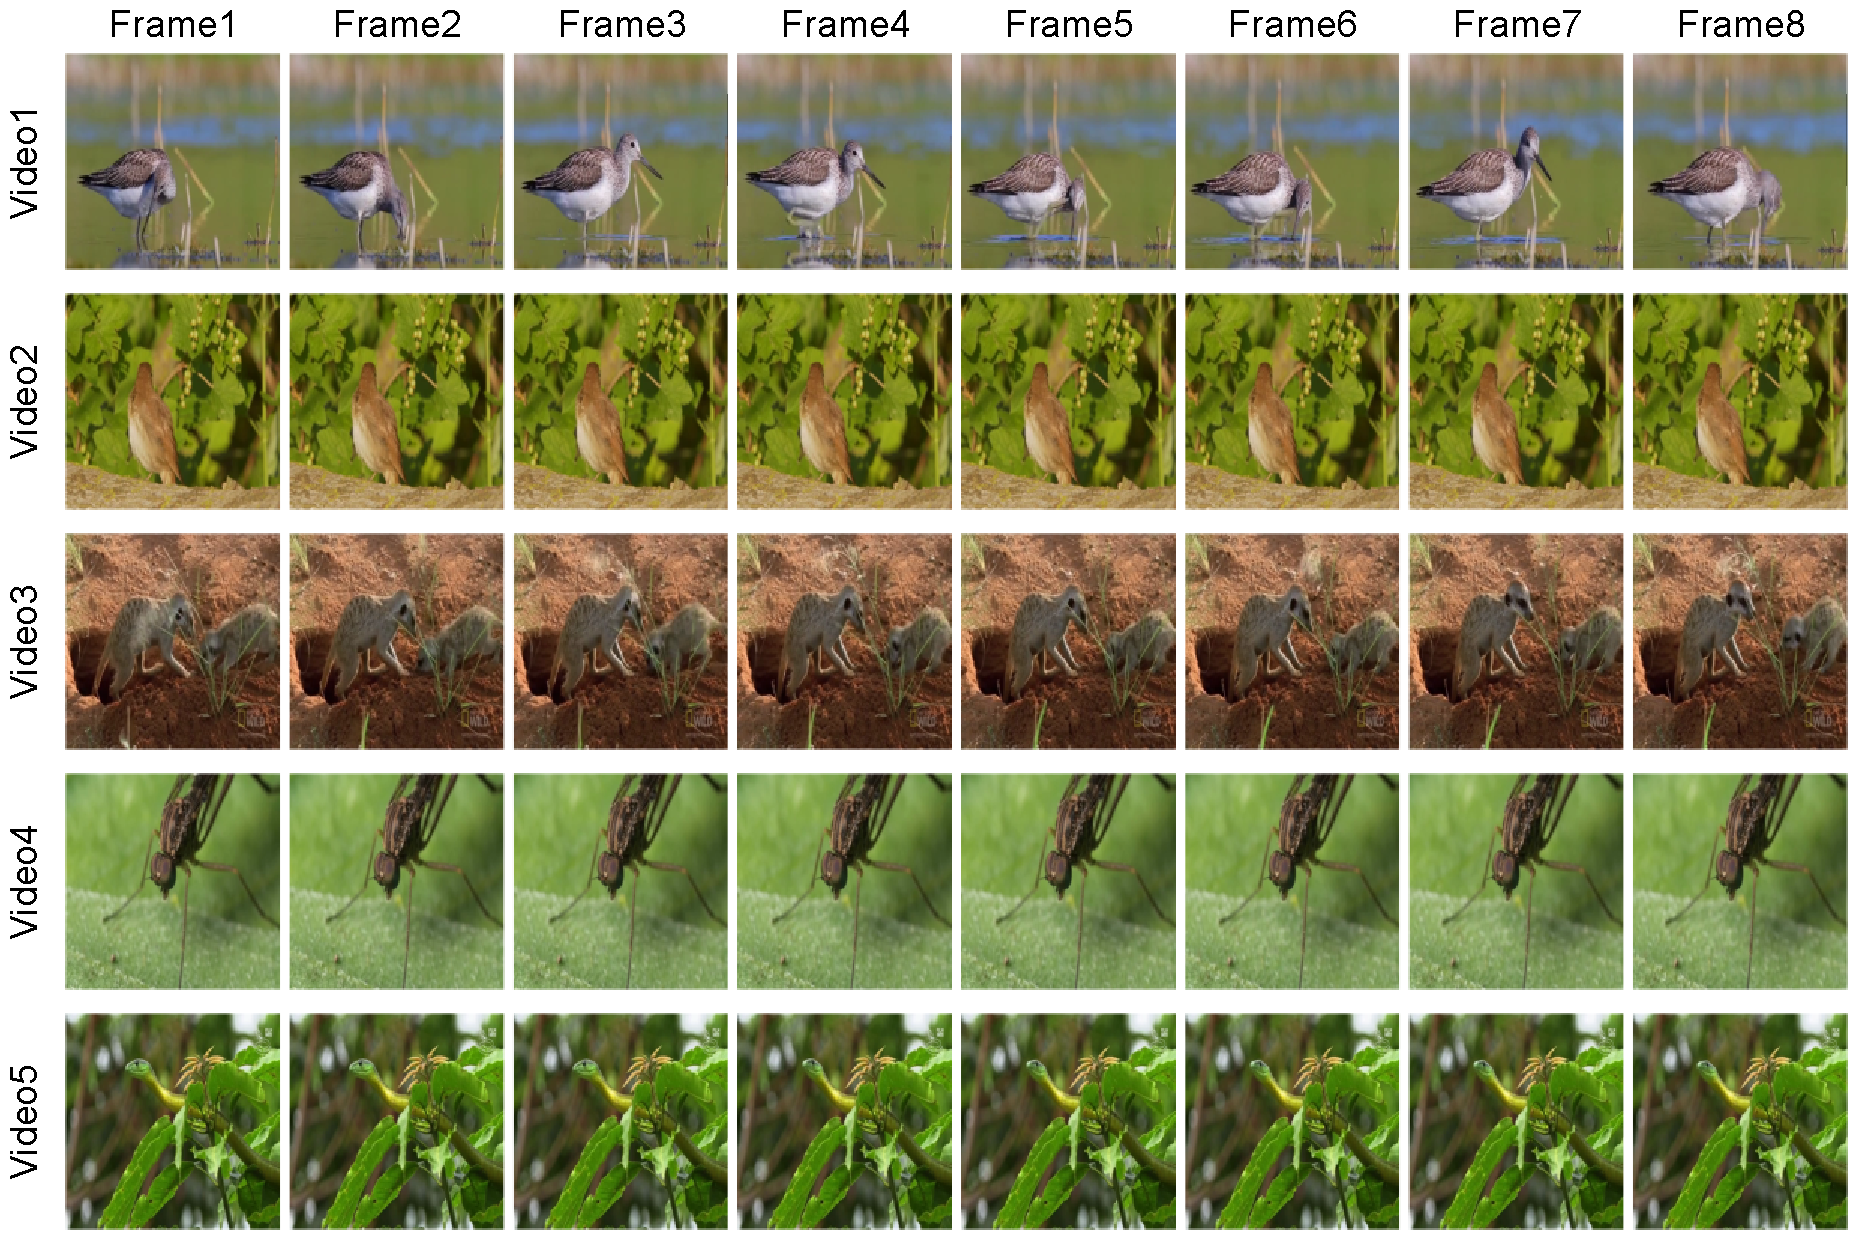
\includegraphics[width=1\textwidth]{assets/imgs/1_2_FrameComparison}
    \caption[Temporal Redundancy]{This figure shows the high temporal redundancy between neighboring frames. Each row of the figure is the sampled frames from the same video. This illustrate the high temporal redundancy in the video.}
    \label{fig:1_2_FrameComparison}
\end{figure}

The second challenge is the temporal redundancy. Since there are a large amount of slow or subtle animal action motions, the high temporal redundancy may confuse the model to do the recognition correctly \parencite{YUAN2018221, li2022uniformer}. Figure \ref{fig:1_2_FrameComparison} illustrates the high temporal redundancy in animal videos. 

In order to enhance the ability to capture the fine-grained texture difference across neighbouring frames, I proposed Action Frame Contrastive Learning Network (AFRICAN) to force the model to extract different features from different frames in the same video. This network is used as a counterpart of CLIP which focuses more on the semantic meaning, contributing around 1 mAP to the final result.

% TODO (Backbone): the improved score may be changed 
\section{Contributions}
In this research, I have the following contributions. Fitst, I proved that CLIP model is able to resolve long-tail issue effectively. Secondly, AFRICAN can be a auxiliary enhancer to help the model gain a better understanding on the temporal dimension.

% May not be written here: improving the overall mAP from 40.92\% using one-hot encoding to 54.76\% using prompt embedding. 




% \begin{itemize}
%   \item If you use \begin{verbatim}\parencite{...}\end{verbatim} you will get just a reference, which may
%     or may not contain names: \parencite{qian2021}.
%   \item If you use \begin{verbatim}\textcite{...}\end{verbatim} you will get the author names as well: \textcite{qian2021}.
% \end{itemize}

% \lipsum[1-2]

% \section{Yes?}

% \subsection{Maybe no}

%   \lipsum[3]

% \subsection{Definitely not}
%   \lipsum[4]
  
% \section{What else?}
%   \lipsum[5-13]


\chapter{Related Work}

  \section{Long-Tail Issue}
In previous research, three main groups of techniques have been employed to deal with the long-tail issue: Re-weighting, Re-sampling, and Few-Shot Learning.

\subsection{Re-weighting}
Re-weighting is a technique used to apply varying weights of penalty to specific groups of classes or samples. This is typically achieved by modifying the loss function. The most vanilla re-weighting scheme involves applying the inverse class frequency to the loss. In this manner, more frequent classes receive a lower weight of loss, enabling the model to put more emphasis on the tail classes \parencite{khan2017cost, mostajabi2015feedforward}.

However, it has been proved that as the number of samples increases, the marginal benefit of model performance diminishes. As a result, directly applying the inverse class frequency to the loss function may excessively reduce the weight of losses for the frequent classes. Class Balanced Loss (CB Loss) has been proposed to resolve this issue. CB Loss calculates the effective number of samples to balance the inverse class frequency, yielding a more reasonable weight for the loss \parencite{cui2019class}.

In contrast to frequency-based re-weighting, Focal Loss focuses on the level of learning difficulties. It scales the penalty to automatically down-weight the contribution of easy examples, which enforces the model to focus on the hard examples \parencite{lin2017focal}.

Label-Distribution-Aware Margin (LDAM) Loss, inspired by hinge loss in support vector machine, ensures that the model has a closer decision boundary when classifying frequent classes. This means that the model must output a higher confidence probability to achieve a better score \parencite{cao2019learning}.

% TODO: some connectivity should be added here
In the context of videos, re-weighting may not be the best strategy to overcome the long-tail issue. Considering the varying amounts of information in a single video, adjusting the weights to tail classes is likely to introduce noise into the training process \parencite{zhang2021videolt}. 

\subsection{Re-sampling}
Re-sampling refers to the intuitive use of sampling algorithms to balance the number of samples for each class. Several early research studies have applied this technique to enhance the model performance \parencite{shen2016relay, 5128907, mahajan2018exploring}.

Previous research has also found that data imbalance itself does not affect the performance of representation learning. Although re-sampling has led to better performance in classification results, it actually benefits classifier learning while harming representation learning. Consequently, subsequent research has focused more on re-sampling techniques used in classifier training \parencite{zhou2020bbn, kang2019decoupling}.

Compared to the previous method that focused on re-sampling algorithms, subsequent research has attempted to reconstruct more samples. VideoLT, for example, concatenates frames from different videos to generate more tail samples \parencite{zhang2021videolt}. Reconstruction of samples in the embedding space has also been explored \parencite{liu2022long, perrett2023use}.

These re-sampling techniques certainly mitigate poor performance in the tail classes. Nevertheless, they do not guarantee the production of samples with the same variety and correctness as the collected data.

\subsection{Few-Shot Learning}
More recent research is concentrating on learning techniques that require fewer training data to achieve acceptable performance.

Model-Agnostic Meta-Learning (Moco) \parencite{finn2017model} proposed the concept of learning to initialise better parameters for training. This has led to a series of studies on meta-learning. Apart from initialisation \parencite{nichol2018first, 2018Reptile}, a large amount of research has begun to apply meta-learning to search for different hyperparameters such as optimization techniques \parencite{andrychowicz2016learning}, data augmentation \parencite{li2020dada, galashov2022data, cubuk2018autoaugment}, and even re-weighting strategies \parencite{shu2019meta}.

With the ability to learn from the small size of data, few-shot learning techniques can also mitigate the long-tail issue. MetaModelNet, for example, regresses the parameters from models trained with less data to the parameters from models trained with more data \parencite{NIPS2017_147ebe63}. Besides, some studies have shown that augmentation or memory retrieval in the embedding space are effective ways to handle tail classes \parencite{liu2019large, Zhu_2020_CVPR, li2021metasaug, Fu_2022_ACCV}.

These methods either focus on few-shot learning or generalise the representation learned from the head classes to the tail classes. In contrast with these methods, Contrastive Vision-Language Pre-training (CLIP) \parencite{radford2021learning} embed both images and sentences into the same semantic space. This enables the model to truly leverage human intelligence to understand visual data as well as balance the distribution of learning targets \parencite{ma2022x}. 

With these advantages, CLIP has been utilised in several image downstream tasks including few-shot learning \parencite{zhang2022tip}, segmentation \parencite{wang2022cris}, video retrieval \parencite{ma2022x}, object detection \parencite{lin2023gridclip}, and captioning \parencite{mokady2021clipcap}. In addition, CLIP for videos has also been proposed \parencite{xu-etal-2021-videoclip, wang2022internvideo}, achieving state-of-the-art results in several video downstream tasks such as classification, video retrieval, and vision question answering.

This research focuses on the long-tail issue and has demonstrated that the text encoder of pretrained CLIP is an efficient tool to overcome the scarcity problem of tail classes.


\section{Temporal Redundancy}
It is shown that boundaries of objects in frames or any small displacements between neighbouring frames are significant features for action recognition \parencite{10.1007/978-3-030-12939-2_20}. In order to enhance the model in this aspect, optical flow and pretext learning are two research directions. 

\subsection{Optical Flow}
In order to capture the tiny boundary changes between frames, it has been popular to utilise the optical flow as an independent stream in the model structure for action recognition \parencite{Piergiovanni_2019_CVPR}. 

Some studies have suggested that optical flow may be replaced or improved due to the expensive computing resources used for its calculation. They proposed another network to substitute the pretrained optical flow model with structural improvements that capture motion between frames, an end-to-end classification network that also predicts the optical flow map. However, although they were more advantageous in terms of the number of model parameters and computation speed, they suffered from inferior performance \parencite{Lee_2018_ECCV, 8354283, Piergiovanni_2019_CVPR}.

\subsection{Pretext Learning}
Some more recent studies focus on designing different pretext tasks for the model to learn in a self-supervised way \parencite{wang2022internvideo}.

Through careful design, the pretext learning model will be able to produce high-quality visual representation in a specific semantic space, which can further be used in downstream tasks such as action recognition, video retrieval, or video captioning \parencite{10.1145/3577925}.

% TODO: should I cite MoCo Again?
Some studies train the model to predict the appearance statistics \parencite{Wang_2019_CVPR}, rotation angles \parencite{DBLP:journals/corr/abs-1811-11387}, playback speed \parencite{Yao_2020_CVPR, 10.1007/978-3-030-58520-4_30}, and temporal order \parencite{10.1007/978-3-030-58604-1_26}. Another way to design a pretext task is to train a contrastive learning model to distinguish if two augmented images are from the same source or not. MoCo \parencite{finn2017model} and SimCLR \parencite{pmlr-v119-chen20j}, proposed to train on image data, are also introduced to video area \parencite{Feichtenhofer_2021_CVPR}.

Inspired by SimCLR, an Action Frame Contrastive Learning Network (AFRICAN) is proposed in this research to force the model to capture the fine-grained difference between frames in a video. In the pretraining stage of AFRICAN, frames in a video are augmented into two different views to do contrastive learning. The target of the contrastive learning model is to identify pairs of frames from the same frame source. This way, the model is able to explore weights that can capture the fine-grained difference between frames. 



\chapter{Methodology}

  In this section, CLIP with prompt engineering for animal action recognition has been explored to solve the long-tail issue, while AFRICAN has been proposed to deal with temporal redundancy. 

\section{CLIP with Prompt Engineering}

\begin{figure}[ht]
    \centering
    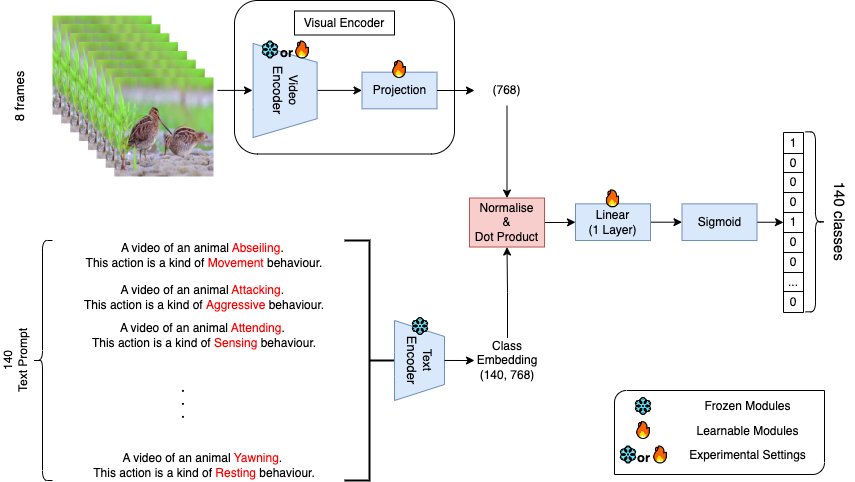
\includegraphics[width=1.0\textwidth]{assets/charts/3_1_ModelStructureVC}
    \caption[VideoCLIP model structure]{This chart illustrates VideoCLIP model structure.}
    \label{fig:modelstructure_vc}
\end{figure}

\begin{figure}[ht]
    \centering
    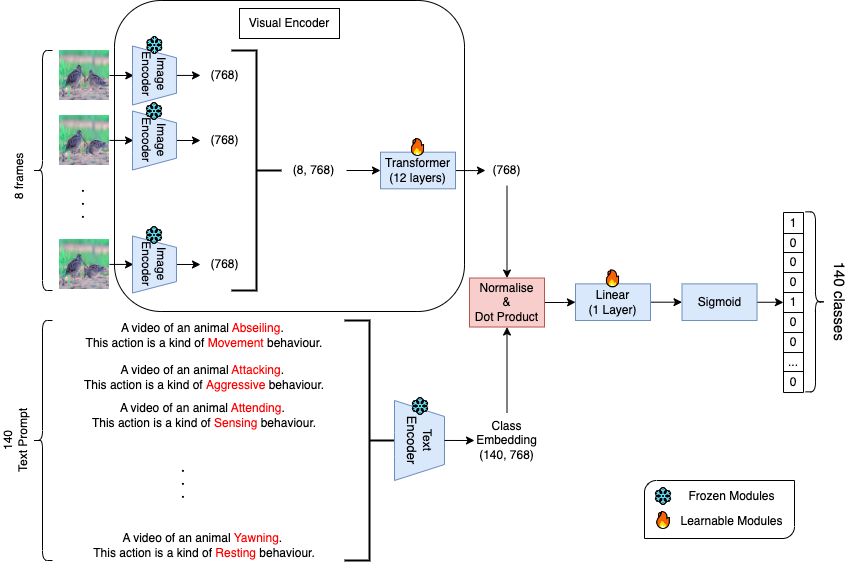
\includegraphics[width=1.0\textwidth]{assets/charts/3_2_ModelStructureIC}
    \caption[ImageCLIP Model Structure]{This chart illustrates ImageCLIP model structure.}
    \label{fig:modelstructure_ic}
\end{figure}

Two model structures are employed for testing the performance of action recognition: 
\begin{enumerate}
    \item VideoCLIP: CLIP pretrained on videos, the clip module of InternVideo \parencite{wang2022internvideo} is used here. The whole structure is illustrated in Figure \ref{fig:modelstructure_vc}.
    \item ImageCLIP: CLIP pretrained on images, the original CLIP \parencite{radford2021learning} is used here. The whole model structure is illustrated in Figure \ref{fig:modelstructure_ic}.
\end{enumerate}

Both models utilise CLIP and prompt engineering for action recognition, taking videos and text prompts as input. The prompt template "A video of an animal
<action>. This action is a kind of <category of action> behaviour." is employed to generate the prompt for producing class embeddings. As shown in Figure \ref{fig:1_2_ClassEmbeddingInternVideo}, this method can produce meaningful distributed class embeddings.

Before training begins, in order to accelerate the process, the class embeddings of size $(140, 768)$ are pre-calculated by a text encoder pretrained by InternVideo based on the prompt template, action name, and category. This is done since the text encoder is frozen, and the weights are not updated. 

Figure \ref{fig:modelstructure_vc} shows the model structure of VideoCLIP. In order to evaluate the structure fairly, two model settings are experimented with on this structure: VideoCLIP training on all vision layers, and VideoCLIP training only on projection layers. Figure \ref{fig:modelstructure_ic} shows the model structure of ImageCLIP. In order to encode the 8 frames into video embeddings, 8 image embeddings encoded by the image encoder of ImageCLIP should be further passed through a 12-layer transformer followed by a pooling layer to produce a 768-dimensional video embedding.

As this is a multilabel classification task, meaning that a video may belong to more than one class, a linear layer is added as a buffer to help the model fit better. Finally, the output logits of the linear layer are then passed through a sigmoid function to determine the probability of each class. 

\section{AFRICAN}
The whole AFRICAN consists of two stages: the pretraining stage and the action recognition stage. The pretraining stage is to train the model to distinguish whether two images are augmented from the same frame in a video or not. At the action recognition stage, the pretrained AFRICAN image encoder is applied to extract the embeddings for action recognition. 

\subsection{Pretraining Stage}

\begin{figure}[ht]
    \centering
    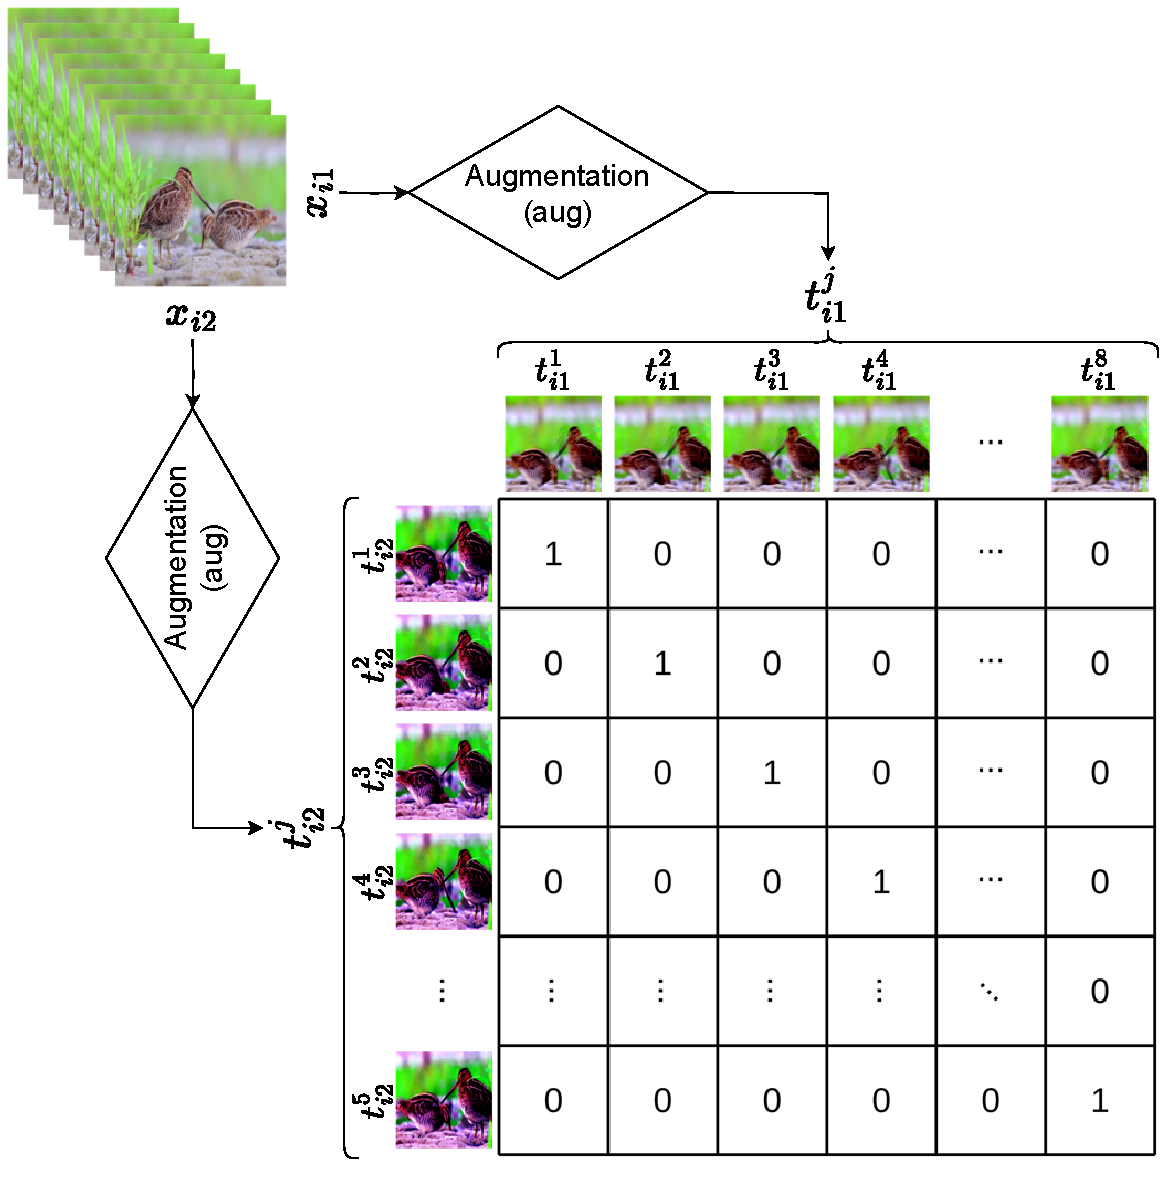
\includegraphics[width=0.6\textwidth]{assets/charts/3_3_ConstrastiveSimilarityMatrix}
    \caption[Operation of pretraining AFRICAN]{This chart illustrates the operation of pretraining AFRICAN.}
f\label{fig:modelstructafsim}
\end{figure}

At the pretraining stage, AFRICAN applies contrastive learning techniques to distinguish whether two images are augmented from the same frame in a video or not. Figure \ref{fig:modelstructafsim} illustrates the batch operation of the model. The input for forwarding is a video sample $x_i$, where $i$ denotes the $i$-th sample in the dataset. $x_i$ is then copied twice into $x_{i1}$ and $x_{i2}$, which then independently pass through the same video augmentation function $aug(\cdot)$ with different random state, as shown in Equations \ref{eq:aug1} and \ref{eq:aug2}. 

\begin{equation}
    \label{eq:aug1}
    t_{i1} = aug(x_{i1})
\end{equation}
\begin{equation}
    \label{eq:aug2}
    t_{i2} = aug(x_{i2})
\end{equation}

After the transformation, $t_{i1}$ and $t_{i2}$ are separated into $j$ frames, denoted as $t_{i1}^j$ and $t_{i2}^j$. In this research, 8 frames are sampled from a video in a batch. Each frame will go through the same image encoder $f(\cdot)$ to be encoded into embeddings $e_{i1}^j$ and $e_{i2}^j$, as shown in Equations \ref{eq:enc1} and \ref{eq:enc2}.

\begin{equation}
    \label{eq:enc1}
    e_{i1}^j = f(t_{i1}^j)
\end{equation}
\begin{equation}
    \label{eq:enc2}
    e_{i2}^j = f(t_{i2}^j)
\end{equation}

Afterwards, the similarity between the image embeddings is calculated by normalisation and dot product, as shown in Equation \ref{eq:sim}, where $k$ denotes the frame index of $e_{i1}$ and $l$ denotes the frame index of $e_{i2}$. The numbers in the matrix in Figure \ref{fig:modelstructafsim} represent the learning targets for different image pair inputs. The diagonal line represents the frame pairs augmented from the same frames, while other numbers indicate pairs of images from different source frames. 

\begin{equation}
    \label{eq:sim}
    t_{i}^{kl} = norm(e_{i1}^{k}) \cdot norm(e_{i2}^{l})
\end{equation}




\subsection{Action Recognition Stage}

\begin{figure}[ht]
    \centering
    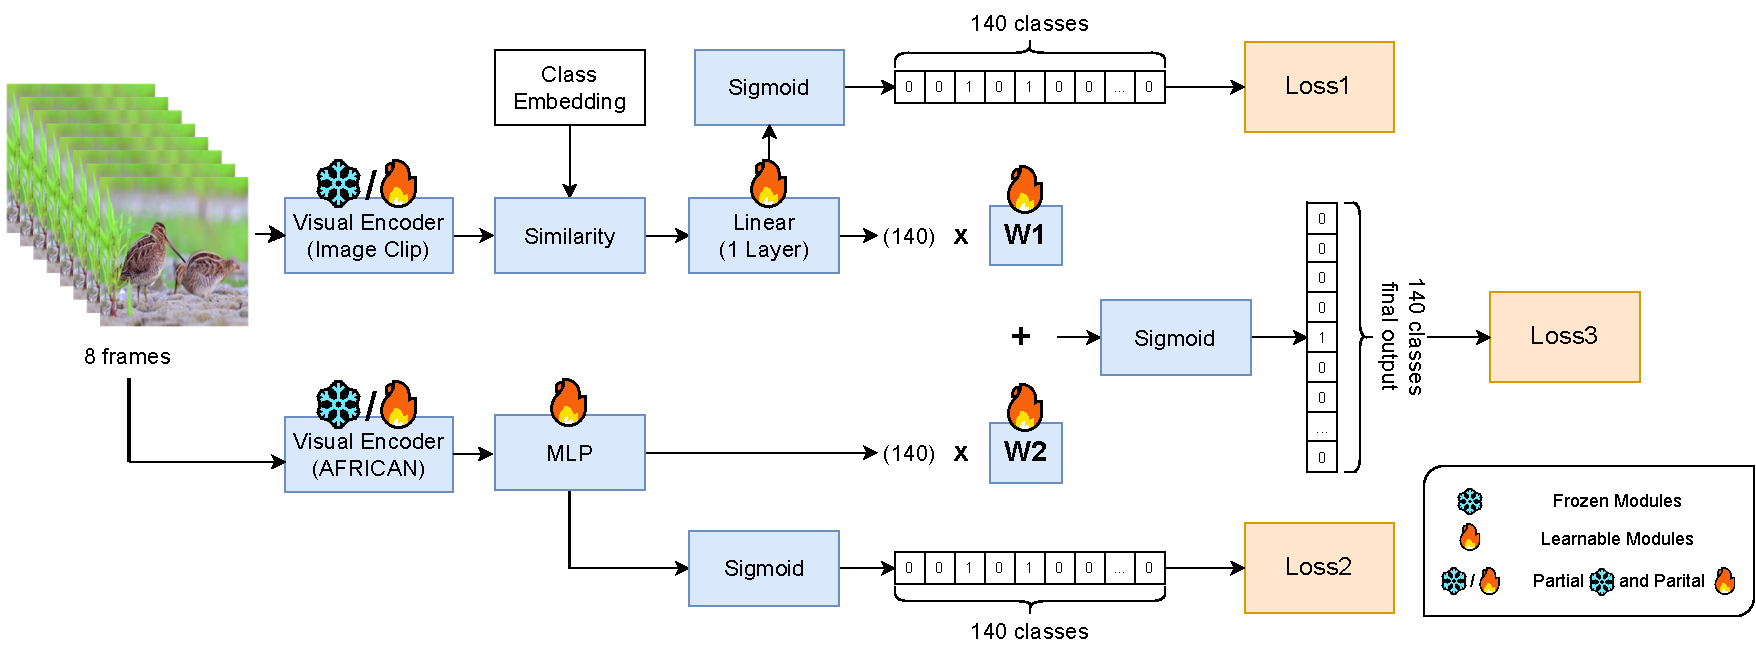
\includegraphics[width=1.0\textwidth]{assets/charts/3_4_ModelStructureAF}
    \caption[Operation of AFRICAN for action recognition]{This chart illustrates the operation of AFRICAN for action recognition.}
    \label{fig:modelstructaf_ar}
\end{figure}

% TODO: further discussion is in the ablation study
Figure \ref{fig:modelstructaf_ar} illustrates the operation of AFRICAN for action recognition. The whole structure consists of two streams. The upper stream is the pretrained CLIP stream, the lower stream is the pretrained AFRICAN stream. 

In the pretrained CLIP stream, the visual encoder and class embedding are the same as those in ImageCLIP, as shown in Figure \ref{fig:modelstructure_ic}. Because the structure of ImageCLIP is able to achieve better performance than VideoCLIP, which will be discussed in Section \ref{sec:imageclipbetter}, ImageCLIP is employed here as the visual encoder in the pretrained CLIP stream. 

In the pretrained AFRICAN stream, the structure of the visual encoder is the same as those in the pretrained CLIP stream but with AFRICAN pretrained weights. Since AFRICAN is not pretrained by the vision-text multimodal model like CLIP, there is no corresponding class embedding. Therefore, a commonly used structure, the multilayer perceptron (MLP), is employed to map the embedding and one-hot encoding. The 3-layer MLP takes the video embedding as input and outputs 140-dimensional logits, which are then passed through a sigmoid function for classification.

After the logits, the input of the sigmoid function, are obtained in the two streams, they are used separately for prediction and computation of loss1 and loss2. Simultaneously, the logits of both streams are multiplied by W1 and W2, two 140-dimensional weights, respectively to determine the contributions of each class for both streams. This is followed by an addition to produce the final prediction and computation of loss3. Finally, loss1, loss2, and loss3 are added together to do the backpropagation. 


\chapter{Experiment}

  In this section, the effectiveness of CLIP with prompt engineering for the long-tail issue and AFRICAN for the temporal redundancy problem will be experimented.

\section {Baseline Model}
The Animal Kingdom dataset also proposed its own model, Collaborative Action Recognition (CARe), for action recognition, which is used as the baseline model in this research. It can achieve 30.55 on overall mAP, 63.33 mAP for head classes, 38.62 for middle classes, and 25.09 for tail classes. This model will be mainly used as the baseline model for animal action recognition in this research.

\section{CLIP with Prompt Engineering}
Before entering the experiment on the long-tail issue, a preliminary decision needs to be made regarding the selection between VideoCLIP and ImageCLIP for action recognition. Subsequently, an examination is undertaken to assess the effectiveness of CLIP in mitigating the long-tail issue.

\subsection{VideoCLIP or ImageCLIP?}
\label{sec:imageclipbetter}
 To make this decision, three model settings are experimented with: 

\begin{enumerate}
    \item VC\_Vision: VideoCLIP with vision layers learnable, as illustrated in Figure \ref{fig:modelstructure_vc} with a learnable video encoder.
    \item VC\_Proj: VideoCLIP with only projection layers learnable, as illustrated in Figure \ref{fig:modelstructure_vc} with a frozen video encoder.
    \item IC: Image CLIP trained on post-transformer layers, as illustrated in Figure \ref{fig:modelstructure_ic} with a frozen image encoder.
\end{enumerate}

For all three of these experiments, the models are trained for 80 epochs on a single A100 GPU, with a binary cross-entropy loss function, the adamw optimizer, and a learning rate of 0.00015. The VC\_Vision model employed a batch size of 16, owing to memory constraints, while batch sizes of 128 were used for the VC\_Proj and IC models. In accordance with Animal Kingdom settings as referenced from \parencite{ng2022animal}, the evaluation metrics used for this task include the mean Average Precision (mAP) on the overall, head, middle, and tail classes, as provided by the dataset. 

% TODO
%The effect of batch size for Video CLIP will be further discussed in Section \ref{sec:ablation_bs}.

The results of the three experiments are shown in Table \ref{tab:resultsbackbone}, and the performance on each epoch during the training process is shown in Figure \ref{fig:tp_backbone}. As illustrated in the figure, the IC model significantly outperforms the other two models. Specifically, the VC\_vision model achieves a 27.19\% mAP on the overall dataset, the lowest among all the experiments. The VC\_Proj model attains a 49.86\% mAP on the overall dataset, making it the second lowest among all the experiments. Conversely, the IC model achieves a 54.79\% mAP on the overall dataset, the highest among all the other experiments. Although both the IC and VC\_Proj models already outperform the baseline model, CARe, which registers a 30.55\% mAP on the overall dataset, the IC model surpasses the VC\_Proj model by 4.81\% mAP on the overall dataset. Therefore, the IC model is selected for the following experiments. For further discussion about the performance of Image CLIP and Video CLIP, please refer to Section \ref{sec:ablation_vc}.

\begin{table}[ht]
    \centering
    \caption{Training Results for Visual Encoder Selection}
    \label{tab:resultsbackbone}
    \begin{tabular}{lllll}
        \toprule
        \multirow{2}{*}{Models} & \multicolumn{4}{c}{mAP} \\
        \cmidrule{2-5} 
        {} & Overall & Head  & Middle & Tail \\
        \midrule
        CARe        & 30.55   & 63.33 & 38.62 & 25.09 \\
        VC\_Vision  & 27.20   & 46.24 & 37.25 & 20.00 \\
        VC\_Proj    & 49.82   & 59.48 & 54.93 & 46.03 \\
        IC          & \textbf{54.36} & \textbf{71.72} & \textbf{63.80} & \textbf{49.07} \\
        \bottomrule
    \end{tabular}
\end{table}


\begin{figure}[ht]
    \centering
    % 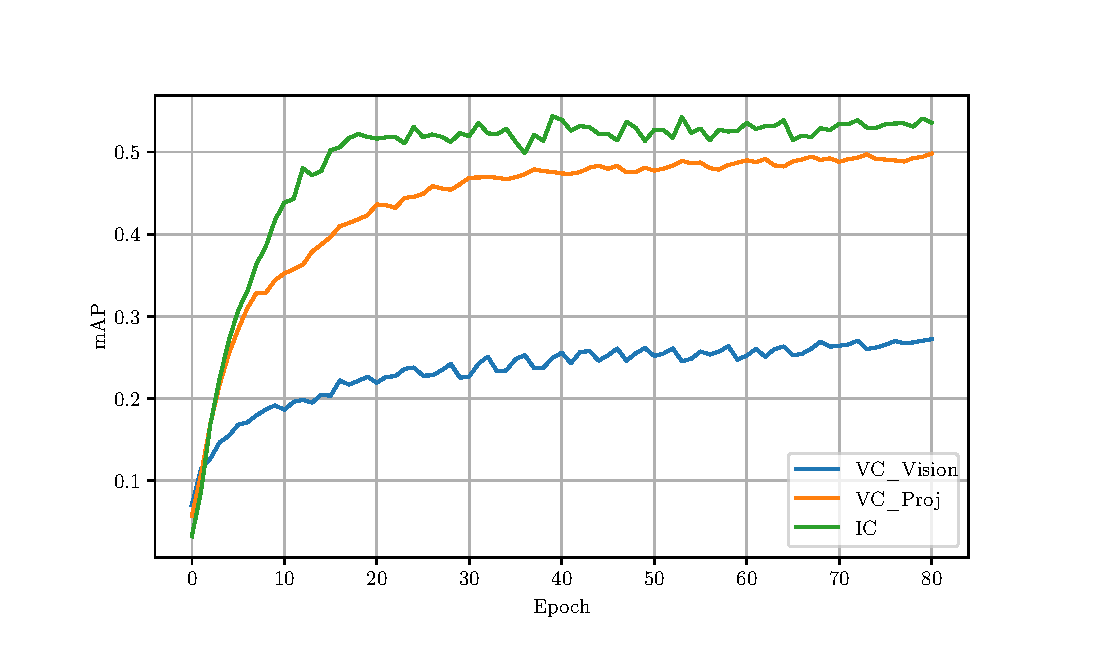
\includegraphics[width=1.0\textwidth]{assets/charts/4_1_BackboneSelection.pgf}
    \resizebox{1.0\textwidth}{!}{%% Creator: Matplotlib, PGF backend
%%
%% To include the figure in your LaTeX document, write
%%   \input{<filename>.pgf}
%%
%% Make sure the required packages are loaded in your preamble
%%   \usepackage{pgf}
%%
%% and, on pdftex
%%   \usepackage[utf8]{inputenc}\DeclareUnicodeCharacter{2212}{-}
%%
%% or, on luatex and xetex
%%   \usepackage{unicode-math}
%%
%% Figures using additional raster images can only be included by \input if
%% they are in the same directory as the main LaTeX file. For loading figures
%% from other directories you can use the `import` package
%%   \usepackage{import}
%%
%% and then include the figures with
%%   \import{<path to file>}{<filename>.pgf}
%%
%% Matplotlib used the following preamble
%%
\begingroup%
\makeatletter%
\begin{pgfpicture}%
\pgfpathrectangle{\pgfpointorigin}{\pgfqpoint{7.000000in}{4.000000in}}%
\pgfusepath{use as bounding box, clip}%
\begin{pgfscope}%
\pgfsetbuttcap%
\pgfsetmiterjoin%
\definecolor{currentfill}{rgb}{1.000000,1.000000,1.000000}%
\pgfsetfillcolor{currentfill}%
\pgfsetlinewidth{0.000000pt}%
\definecolor{currentstroke}{rgb}{1.000000,1.000000,1.000000}%
\pgfsetstrokecolor{currentstroke}%
\pgfsetdash{}{0pt}%
\pgfpathmoveto{\pgfqpoint{0.000000in}{0.000000in}}%
\pgfpathlineto{\pgfqpoint{7.000000in}{0.000000in}}%
\pgfpathlineto{\pgfqpoint{7.000000in}{4.000000in}}%
\pgfpathlineto{\pgfqpoint{0.000000in}{4.000000in}}%
\pgfpathclose%
\pgfusepath{fill}%
\end{pgfscope}%
\begin{pgfscope}%
\pgfsetbuttcap%
\pgfsetmiterjoin%
\definecolor{currentfill}{rgb}{1.000000,1.000000,1.000000}%
\pgfsetfillcolor{currentfill}%
\pgfsetlinewidth{0.000000pt}%
\definecolor{currentstroke}{rgb}{0.000000,0.000000,0.000000}%
\pgfsetstrokecolor{currentstroke}%
\pgfsetstrokeopacity{0.000000}%
\pgfsetdash{}{0pt}%
\pgfpathmoveto{\pgfqpoint{0.875000in}{0.440000in}}%
\pgfpathlineto{\pgfqpoint{6.300000in}{0.440000in}}%
\pgfpathlineto{\pgfqpoint{6.300000in}{3.520000in}}%
\pgfpathlineto{\pgfqpoint{0.875000in}{3.520000in}}%
\pgfpathclose%
\pgfusepath{fill}%
\end{pgfscope}%
\begin{pgfscope}%
\pgfpathrectangle{\pgfqpoint{0.875000in}{0.440000in}}{\pgfqpoint{5.425000in}{3.080000in}}%
\pgfusepath{clip}%
\pgfsetrectcap%
\pgfsetroundjoin%
\pgfsetlinewidth{0.803000pt}%
\definecolor{currentstroke}{rgb}{0.690196,0.690196,0.690196}%
\pgfsetstrokecolor{currentstroke}%
\pgfsetdash{}{0pt}%
\pgfpathmoveto{\pgfqpoint{1.121591in}{0.440000in}}%
\pgfpathlineto{\pgfqpoint{1.121591in}{3.520000in}}%
\pgfusepath{stroke}%
\end{pgfscope}%
\begin{pgfscope}%
\pgfsetbuttcap%
\pgfsetroundjoin%
\definecolor{currentfill}{rgb}{0.000000,0.000000,0.000000}%
\pgfsetfillcolor{currentfill}%
\pgfsetlinewidth{0.803000pt}%
\definecolor{currentstroke}{rgb}{0.000000,0.000000,0.000000}%
\pgfsetstrokecolor{currentstroke}%
\pgfsetdash{}{0pt}%
\pgfsys@defobject{currentmarker}{\pgfqpoint{0.000000in}{-0.048611in}}{\pgfqpoint{0.000000in}{0.000000in}}{%
\pgfpathmoveto{\pgfqpoint{0.000000in}{0.000000in}}%
\pgfpathlineto{\pgfqpoint{0.000000in}{-0.048611in}}%
\pgfusepath{stroke,fill}%
}%
\begin{pgfscope}%
\pgfsys@transformshift{1.121591in}{0.440000in}%
\pgfsys@useobject{currentmarker}{}%
\end{pgfscope}%
\end{pgfscope}%
\begin{pgfscope}%
\definecolor{textcolor}{rgb}{0.000000,0.000000,0.000000}%
\pgfsetstrokecolor{textcolor}%
\pgfsetfillcolor{textcolor}%
\pgftext[x=1.121591in,y=0.342778in,,top]{\color{textcolor}\rmfamily\fontsize{10.000000}{12.000000}\selectfont \(\displaystyle {0}\)}%
\end{pgfscope}%
\begin{pgfscope}%
\pgfpathrectangle{\pgfqpoint{0.875000in}{0.440000in}}{\pgfqpoint{5.425000in}{3.080000in}}%
\pgfusepath{clip}%
\pgfsetrectcap%
\pgfsetroundjoin%
\pgfsetlinewidth{0.803000pt}%
\definecolor{currentstroke}{rgb}{0.690196,0.690196,0.690196}%
\pgfsetstrokecolor{currentstroke}%
\pgfsetdash{}{0pt}%
\pgfpathmoveto{\pgfqpoint{1.738068in}{0.440000in}}%
\pgfpathlineto{\pgfqpoint{1.738068in}{3.520000in}}%
\pgfusepath{stroke}%
\end{pgfscope}%
\begin{pgfscope}%
\pgfsetbuttcap%
\pgfsetroundjoin%
\definecolor{currentfill}{rgb}{0.000000,0.000000,0.000000}%
\pgfsetfillcolor{currentfill}%
\pgfsetlinewidth{0.803000pt}%
\definecolor{currentstroke}{rgb}{0.000000,0.000000,0.000000}%
\pgfsetstrokecolor{currentstroke}%
\pgfsetdash{}{0pt}%
\pgfsys@defobject{currentmarker}{\pgfqpoint{0.000000in}{-0.048611in}}{\pgfqpoint{0.000000in}{0.000000in}}{%
\pgfpathmoveto{\pgfqpoint{0.000000in}{0.000000in}}%
\pgfpathlineto{\pgfqpoint{0.000000in}{-0.048611in}}%
\pgfusepath{stroke,fill}%
}%
\begin{pgfscope}%
\pgfsys@transformshift{1.738068in}{0.440000in}%
\pgfsys@useobject{currentmarker}{}%
\end{pgfscope}%
\end{pgfscope}%
\begin{pgfscope}%
\definecolor{textcolor}{rgb}{0.000000,0.000000,0.000000}%
\pgfsetstrokecolor{textcolor}%
\pgfsetfillcolor{textcolor}%
\pgftext[x=1.738068in,y=0.342778in,,top]{\color{textcolor}\rmfamily\fontsize{10.000000}{12.000000}\selectfont \(\displaystyle {10}\)}%
\end{pgfscope}%
\begin{pgfscope}%
\pgfpathrectangle{\pgfqpoint{0.875000in}{0.440000in}}{\pgfqpoint{5.425000in}{3.080000in}}%
\pgfusepath{clip}%
\pgfsetrectcap%
\pgfsetroundjoin%
\pgfsetlinewidth{0.803000pt}%
\definecolor{currentstroke}{rgb}{0.690196,0.690196,0.690196}%
\pgfsetstrokecolor{currentstroke}%
\pgfsetdash{}{0pt}%
\pgfpathmoveto{\pgfqpoint{2.354545in}{0.440000in}}%
\pgfpathlineto{\pgfqpoint{2.354545in}{3.520000in}}%
\pgfusepath{stroke}%
\end{pgfscope}%
\begin{pgfscope}%
\pgfsetbuttcap%
\pgfsetroundjoin%
\definecolor{currentfill}{rgb}{0.000000,0.000000,0.000000}%
\pgfsetfillcolor{currentfill}%
\pgfsetlinewidth{0.803000pt}%
\definecolor{currentstroke}{rgb}{0.000000,0.000000,0.000000}%
\pgfsetstrokecolor{currentstroke}%
\pgfsetdash{}{0pt}%
\pgfsys@defobject{currentmarker}{\pgfqpoint{0.000000in}{-0.048611in}}{\pgfqpoint{0.000000in}{0.000000in}}{%
\pgfpathmoveto{\pgfqpoint{0.000000in}{0.000000in}}%
\pgfpathlineto{\pgfqpoint{0.000000in}{-0.048611in}}%
\pgfusepath{stroke,fill}%
}%
\begin{pgfscope}%
\pgfsys@transformshift{2.354545in}{0.440000in}%
\pgfsys@useobject{currentmarker}{}%
\end{pgfscope}%
\end{pgfscope}%
\begin{pgfscope}%
\definecolor{textcolor}{rgb}{0.000000,0.000000,0.000000}%
\pgfsetstrokecolor{textcolor}%
\pgfsetfillcolor{textcolor}%
\pgftext[x=2.354545in,y=0.342778in,,top]{\color{textcolor}\rmfamily\fontsize{10.000000}{12.000000}\selectfont \(\displaystyle {20}\)}%
\end{pgfscope}%
\begin{pgfscope}%
\pgfpathrectangle{\pgfqpoint{0.875000in}{0.440000in}}{\pgfqpoint{5.425000in}{3.080000in}}%
\pgfusepath{clip}%
\pgfsetrectcap%
\pgfsetroundjoin%
\pgfsetlinewidth{0.803000pt}%
\definecolor{currentstroke}{rgb}{0.690196,0.690196,0.690196}%
\pgfsetstrokecolor{currentstroke}%
\pgfsetdash{}{0pt}%
\pgfpathmoveto{\pgfqpoint{2.971023in}{0.440000in}}%
\pgfpathlineto{\pgfqpoint{2.971023in}{3.520000in}}%
\pgfusepath{stroke}%
\end{pgfscope}%
\begin{pgfscope}%
\pgfsetbuttcap%
\pgfsetroundjoin%
\definecolor{currentfill}{rgb}{0.000000,0.000000,0.000000}%
\pgfsetfillcolor{currentfill}%
\pgfsetlinewidth{0.803000pt}%
\definecolor{currentstroke}{rgb}{0.000000,0.000000,0.000000}%
\pgfsetstrokecolor{currentstroke}%
\pgfsetdash{}{0pt}%
\pgfsys@defobject{currentmarker}{\pgfqpoint{0.000000in}{-0.048611in}}{\pgfqpoint{0.000000in}{0.000000in}}{%
\pgfpathmoveto{\pgfqpoint{0.000000in}{0.000000in}}%
\pgfpathlineto{\pgfqpoint{0.000000in}{-0.048611in}}%
\pgfusepath{stroke,fill}%
}%
\begin{pgfscope}%
\pgfsys@transformshift{2.971023in}{0.440000in}%
\pgfsys@useobject{currentmarker}{}%
\end{pgfscope}%
\end{pgfscope}%
\begin{pgfscope}%
\definecolor{textcolor}{rgb}{0.000000,0.000000,0.000000}%
\pgfsetstrokecolor{textcolor}%
\pgfsetfillcolor{textcolor}%
\pgftext[x=2.971023in,y=0.342778in,,top]{\color{textcolor}\rmfamily\fontsize{10.000000}{12.000000}\selectfont \(\displaystyle {30}\)}%
\end{pgfscope}%
\begin{pgfscope}%
\pgfpathrectangle{\pgfqpoint{0.875000in}{0.440000in}}{\pgfqpoint{5.425000in}{3.080000in}}%
\pgfusepath{clip}%
\pgfsetrectcap%
\pgfsetroundjoin%
\pgfsetlinewidth{0.803000pt}%
\definecolor{currentstroke}{rgb}{0.690196,0.690196,0.690196}%
\pgfsetstrokecolor{currentstroke}%
\pgfsetdash{}{0pt}%
\pgfpathmoveto{\pgfqpoint{3.587500in}{0.440000in}}%
\pgfpathlineto{\pgfqpoint{3.587500in}{3.520000in}}%
\pgfusepath{stroke}%
\end{pgfscope}%
\begin{pgfscope}%
\pgfsetbuttcap%
\pgfsetroundjoin%
\definecolor{currentfill}{rgb}{0.000000,0.000000,0.000000}%
\pgfsetfillcolor{currentfill}%
\pgfsetlinewidth{0.803000pt}%
\definecolor{currentstroke}{rgb}{0.000000,0.000000,0.000000}%
\pgfsetstrokecolor{currentstroke}%
\pgfsetdash{}{0pt}%
\pgfsys@defobject{currentmarker}{\pgfqpoint{0.000000in}{-0.048611in}}{\pgfqpoint{0.000000in}{0.000000in}}{%
\pgfpathmoveto{\pgfqpoint{0.000000in}{0.000000in}}%
\pgfpathlineto{\pgfqpoint{0.000000in}{-0.048611in}}%
\pgfusepath{stroke,fill}%
}%
\begin{pgfscope}%
\pgfsys@transformshift{3.587500in}{0.440000in}%
\pgfsys@useobject{currentmarker}{}%
\end{pgfscope}%
\end{pgfscope}%
\begin{pgfscope}%
\definecolor{textcolor}{rgb}{0.000000,0.000000,0.000000}%
\pgfsetstrokecolor{textcolor}%
\pgfsetfillcolor{textcolor}%
\pgftext[x=3.587500in,y=0.342778in,,top]{\color{textcolor}\rmfamily\fontsize{10.000000}{12.000000}\selectfont \(\displaystyle {40}\)}%
\end{pgfscope}%
\begin{pgfscope}%
\pgfpathrectangle{\pgfqpoint{0.875000in}{0.440000in}}{\pgfqpoint{5.425000in}{3.080000in}}%
\pgfusepath{clip}%
\pgfsetrectcap%
\pgfsetroundjoin%
\pgfsetlinewidth{0.803000pt}%
\definecolor{currentstroke}{rgb}{0.690196,0.690196,0.690196}%
\pgfsetstrokecolor{currentstroke}%
\pgfsetdash{}{0pt}%
\pgfpathmoveto{\pgfqpoint{4.203977in}{0.440000in}}%
\pgfpathlineto{\pgfqpoint{4.203977in}{3.520000in}}%
\pgfusepath{stroke}%
\end{pgfscope}%
\begin{pgfscope}%
\pgfsetbuttcap%
\pgfsetroundjoin%
\definecolor{currentfill}{rgb}{0.000000,0.000000,0.000000}%
\pgfsetfillcolor{currentfill}%
\pgfsetlinewidth{0.803000pt}%
\definecolor{currentstroke}{rgb}{0.000000,0.000000,0.000000}%
\pgfsetstrokecolor{currentstroke}%
\pgfsetdash{}{0pt}%
\pgfsys@defobject{currentmarker}{\pgfqpoint{0.000000in}{-0.048611in}}{\pgfqpoint{0.000000in}{0.000000in}}{%
\pgfpathmoveto{\pgfqpoint{0.000000in}{0.000000in}}%
\pgfpathlineto{\pgfqpoint{0.000000in}{-0.048611in}}%
\pgfusepath{stroke,fill}%
}%
\begin{pgfscope}%
\pgfsys@transformshift{4.203977in}{0.440000in}%
\pgfsys@useobject{currentmarker}{}%
\end{pgfscope}%
\end{pgfscope}%
\begin{pgfscope}%
\definecolor{textcolor}{rgb}{0.000000,0.000000,0.000000}%
\pgfsetstrokecolor{textcolor}%
\pgfsetfillcolor{textcolor}%
\pgftext[x=4.203977in,y=0.342778in,,top]{\color{textcolor}\rmfamily\fontsize{10.000000}{12.000000}\selectfont \(\displaystyle {50}\)}%
\end{pgfscope}%
\begin{pgfscope}%
\pgfpathrectangle{\pgfqpoint{0.875000in}{0.440000in}}{\pgfqpoint{5.425000in}{3.080000in}}%
\pgfusepath{clip}%
\pgfsetrectcap%
\pgfsetroundjoin%
\pgfsetlinewidth{0.803000pt}%
\definecolor{currentstroke}{rgb}{0.690196,0.690196,0.690196}%
\pgfsetstrokecolor{currentstroke}%
\pgfsetdash{}{0pt}%
\pgfpathmoveto{\pgfqpoint{4.820455in}{0.440000in}}%
\pgfpathlineto{\pgfqpoint{4.820455in}{3.520000in}}%
\pgfusepath{stroke}%
\end{pgfscope}%
\begin{pgfscope}%
\pgfsetbuttcap%
\pgfsetroundjoin%
\definecolor{currentfill}{rgb}{0.000000,0.000000,0.000000}%
\pgfsetfillcolor{currentfill}%
\pgfsetlinewidth{0.803000pt}%
\definecolor{currentstroke}{rgb}{0.000000,0.000000,0.000000}%
\pgfsetstrokecolor{currentstroke}%
\pgfsetdash{}{0pt}%
\pgfsys@defobject{currentmarker}{\pgfqpoint{0.000000in}{-0.048611in}}{\pgfqpoint{0.000000in}{0.000000in}}{%
\pgfpathmoveto{\pgfqpoint{0.000000in}{0.000000in}}%
\pgfpathlineto{\pgfqpoint{0.000000in}{-0.048611in}}%
\pgfusepath{stroke,fill}%
}%
\begin{pgfscope}%
\pgfsys@transformshift{4.820455in}{0.440000in}%
\pgfsys@useobject{currentmarker}{}%
\end{pgfscope}%
\end{pgfscope}%
\begin{pgfscope}%
\definecolor{textcolor}{rgb}{0.000000,0.000000,0.000000}%
\pgfsetstrokecolor{textcolor}%
\pgfsetfillcolor{textcolor}%
\pgftext[x=4.820455in,y=0.342778in,,top]{\color{textcolor}\rmfamily\fontsize{10.000000}{12.000000}\selectfont \(\displaystyle {60}\)}%
\end{pgfscope}%
\begin{pgfscope}%
\pgfpathrectangle{\pgfqpoint{0.875000in}{0.440000in}}{\pgfqpoint{5.425000in}{3.080000in}}%
\pgfusepath{clip}%
\pgfsetrectcap%
\pgfsetroundjoin%
\pgfsetlinewidth{0.803000pt}%
\definecolor{currentstroke}{rgb}{0.690196,0.690196,0.690196}%
\pgfsetstrokecolor{currentstroke}%
\pgfsetdash{}{0pt}%
\pgfpathmoveto{\pgfqpoint{5.436932in}{0.440000in}}%
\pgfpathlineto{\pgfqpoint{5.436932in}{3.520000in}}%
\pgfusepath{stroke}%
\end{pgfscope}%
\begin{pgfscope}%
\pgfsetbuttcap%
\pgfsetroundjoin%
\definecolor{currentfill}{rgb}{0.000000,0.000000,0.000000}%
\pgfsetfillcolor{currentfill}%
\pgfsetlinewidth{0.803000pt}%
\definecolor{currentstroke}{rgb}{0.000000,0.000000,0.000000}%
\pgfsetstrokecolor{currentstroke}%
\pgfsetdash{}{0pt}%
\pgfsys@defobject{currentmarker}{\pgfqpoint{0.000000in}{-0.048611in}}{\pgfqpoint{0.000000in}{0.000000in}}{%
\pgfpathmoveto{\pgfqpoint{0.000000in}{0.000000in}}%
\pgfpathlineto{\pgfqpoint{0.000000in}{-0.048611in}}%
\pgfusepath{stroke,fill}%
}%
\begin{pgfscope}%
\pgfsys@transformshift{5.436932in}{0.440000in}%
\pgfsys@useobject{currentmarker}{}%
\end{pgfscope}%
\end{pgfscope}%
\begin{pgfscope}%
\definecolor{textcolor}{rgb}{0.000000,0.000000,0.000000}%
\pgfsetstrokecolor{textcolor}%
\pgfsetfillcolor{textcolor}%
\pgftext[x=5.436932in,y=0.342778in,,top]{\color{textcolor}\rmfamily\fontsize{10.000000}{12.000000}\selectfont \(\displaystyle {70}\)}%
\end{pgfscope}%
\begin{pgfscope}%
\pgfpathrectangle{\pgfqpoint{0.875000in}{0.440000in}}{\pgfqpoint{5.425000in}{3.080000in}}%
\pgfusepath{clip}%
\pgfsetrectcap%
\pgfsetroundjoin%
\pgfsetlinewidth{0.803000pt}%
\definecolor{currentstroke}{rgb}{0.690196,0.690196,0.690196}%
\pgfsetstrokecolor{currentstroke}%
\pgfsetdash{}{0pt}%
\pgfpathmoveto{\pgfqpoint{6.053409in}{0.440000in}}%
\pgfpathlineto{\pgfqpoint{6.053409in}{3.520000in}}%
\pgfusepath{stroke}%
\end{pgfscope}%
\begin{pgfscope}%
\pgfsetbuttcap%
\pgfsetroundjoin%
\definecolor{currentfill}{rgb}{0.000000,0.000000,0.000000}%
\pgfsetfillcolor{currentfill}%
\pgfsetlinewidth{0.803000pt}%
\definecolor{currentstroke}{rgb}{0.000000,0.000000,0.000000}%
\pgfsetstrokecolor{currentstroke}%
\pgfsetdash{}{0pt}%
\pgfsys@defobject{currentmarker}{\pgfqpoint{0.000000in}{-0.048611in}}{\pgfqpoint{0.000000in}{0.000000in}}{%
\pgfpathmoveto{\pgfqpoint{0.000000in}{0.000000in}}%
\pgfpathlineto{\pgfqpoint{0.000000in}{-0.048611in}}%
\pgfusepath{stroke,fill}%
}%
\begin{pgfscope}%
\pgfsys@transformshift{6.053409in}{0.440000in}%
\pgfsys@useobject{currentmarker}{}%
\end{pgfscope}%
\end{pgfscope}%
\begin{pgfscope}%
\definecolor{textcolor}{rgb}{0.000000,0.000000,0.000000}%
\pgfsetstrokecolor{textcolor}%
\pgfsetfillcolor{textcolor}%
\pgftext[x=6.053409in,y=0.342778in,,top]{\color{textcolor}\rmfamily\fontsize{10.000000}{12.000000}\selectfont \(\displaystyle {80}\)}%
\end{pgfscope}%
\begin{pgfscope}%
\definecolor{textcolor}{rgb}{0.000000,0.000000,0.000000}%
\pgfsetstrokecolor{textcolor}%
\pgfsetfillcolor{textcolor}%
\pgftext[x=3.587500in,y=0.163766in,,top]{\color{textcolor}\rmfamily\fontsize{10.000000}{12.000000}\selectfont Epoch}%
\end{pgfscope}%
\begin{pgfscope}%
\pgfpathrectangle{\pgfqpoint{0.875000in}{0.440000in}}{\pgfqpoint{5.425000in}{3.080000in}}%
\pgfusepath{clip}%
\pgfsetrectcap%
\pgfsetroundjoin%
\pgfsetlinewidth{0.803000pt}%
\definecolor{currentstroke}{rgb}{0.690196,0.690196,0.690196}%
\pgfsetstrokecolor{currentstroke}%
\pgfsetdash{}{0pt}%
\pgfpathmoveto{\pgfqpoint{0.875000in}{0.953310in}}%
\pgfpathlineto{\pgfqpoint{6.300000in}{0.953310in}}%
\pgfusepath{stroke}%
\end{pgfscope}%
\begin{pgfscope}%
\pgfsetbuttcap%
\pgfsetroundjoin%
\definecolor{currentfill}{rgb}{0.000000,0.000000,0.000000}%
\pgfsetfillcolor{currentfill}%
\pgfsetlinewidth{0.803000pt}%
\definecolor{currentstroke}{rgb}{0.000000,0.000000,0.000000}%
\pgfsetstrokecolor{currentstroke}%
\pgfsetdash{}{0pt}%
\pgfsys@defobject{currentmarker}{\pgfqpoint{-0.048611in}{0.000000in}}{\pgfqpoint{0.000000in}{0.000000in}}{%
\pgfpathmoveto{\pgfqpoint{0.000000in}{0.000000in}}%
\pgfpathlineto{\pgfqpoint{-0.048611in}{0.000000in}}%
\pgfusepath{stroke,fill}%
}%
\begin{pgfscope}%
\pgfsys@transformshift{0.875000in}{0.953310in}%
\pgfsys@useobject{currentmarker}{}%
\end{pgfscope}%
\end{pgfscope}%
\begin{pgfscope}%
\definecolor{textcolor}{rgb}{0.000000,0.000000,0.000000}%
\pgfsetstrokecolor{textcolor}%
\pgfsetfillcolor{textcolor}%
\pgftext[x=0.600308in, y=0.905085in, left, base]{\color{textcolor}\rmfamily\fontsize{10.000000}{12.000000}\selectfont \(\displaystyle {0.1}\)}%
\end{pgfscope}%
\begin{pgfscope}%
\pgfpathrectangle{\pgfqpoint{0.875000in}{0.440000in}}{\pgfqpoint{5.425000in}{3.080000in}}%
\pgfusepath{clip}%
\pgfsetrectcap%
\pgfsetroundjoin%
\pgfsetlinewidth{0.803000pt}%
\definecolor{currentstroke}{rgb}{0.690196,0.690196,0.690196}%
\pgfsetstrokecolor{currentstroke}%
\pgfsetdash{}{0pt}%
\pgfpathmoveto{\pgfqpoint{0.875000in}{1.500339in}}%
\pgfpathlineto{\pgfqpoint{6.300000in}{1.500339in}}%
\pgfusepath{stroke}%
\end{pgfscope}%
\begin{pgfscope}%
\pgfsetbuttcap%
\pgfsetroundjoin%
\definecolor{currentfill}{rgb}{0.000000,0.000000,0.000000}%
\pgfsetfillcolor{currentfill}%
\pgfsetlinewidth{0.803000pt}%
\definecolor{currentstroke}{rgb}{0.000000,0.000000,0.000000}%
\pgfsetstrokecolor{currentstroke}%
\pgfsetdash{}{0pt}%
\pgfsys@defobject{currentmarker}{\pgfqpoint{-0.048611in}{0.000000in}}{\pgfqpoint{0.000000in}{0.000000in}}{%
\pgfpathmoveto{\pgfqpoint{0.000000in}{0.000000in}}%
\pgfpathlineto{\pgfqpoint{-0.048611in}{0.000000in}}%
\pgfusepath{stroke,fill}%
}%
\begin{pgfscope}%
\pgfsys@transformshift{0.875000in}{1.500339in}%
\pgfsys@useobject{currentmarker}{}%
\end{pgfscope}%
\end{pgfscope}%
\begin{pgfscope}%
\definecolor{textcolor}{rgb}{0.000000,0.000000,0.000000}%
\pgfsetstrokecolor{textcolor}%
\pgfsetfillcolor{textcolor}%
\pgftext[x=0.600308in, y=1.452113in, left, base]{\color{textcolor}\rmfamily\fontsize{10.000000}{12.000000}\selectfont \(\displaystyle {0.2}\)}%
\end{pgfscope}%
\begin{pgfscope}%
\pgfpathrectangle{\pgfqpoint{0.875000in}{0.440000in}}{\pgfqpoint{5.425000in}{3.080000in}}%
\pgfusepath{clip}%
\pgfsetrectcap%
\pgfsetroundjoin%
\pgfsetlinewidth{0.803000pt}%
\definecolor{currentstroke}{rgb}{0.690196,0.690196,0.690196}%
\pgfsetstrokecolor{currentstroke}%
\pgfsetdash{}{0pt}%
\pgfpathmoveto{\pgfqpoint{0.875000in}{2.047367in}}%
\pgfpathlineto{\pgfqpoint{6.300000in}{2.047367in}}%
\pgfusepath{stroke}%
\end{pgfscope}%
\begin{pgfscope}%
\pgfsetbuttcap%
\pgfsetroundjoin%
\definecolor{currentfill}{rgb}{0.000000,0.000000,0.000000}%
\pgfsetfillcolor{currentfill}%
\pgfsetlinewidth{0.803000pt}%
\definecolor{currentstroke}{rgb}{0.000000,0.000000,0.000000}%
\pgfsetstrokecolor{currentstroke}%
\pgfsetdash{}{0pt}%
\pgfsys@defobject{currentmarker}{\pgfqpoint{-0.048611in}{0.000000in}}{\pgfqpoint{0.000000in}{0.000000in}}{%
\pgfpathmoveto{\pgfqpoint{0.000000in}{0.000000in}}%
\pgfpathlineto{\pgfqpoint{-0.048611in}{0.000000in}}%
\pgfusepath{stroke,fill}%
}%
\begin{pgfscope}%
\pgfsys@transformshift{0.875000in}{2.047367in}%
\pgfsys@useobject{currentmarker}{}%
\end{pgfscope}%
\end{pgfscope}%
\begin{pgfscope}%
\definecolor{textcolor}{rgb}{0.000000,0.000000,0.000000}%
\pgfsetstrokecolor{textcolor}%
\pgfsetfillcolor{textcolor}%
\pgftext[x=0.600308in, y=1.999141in, left, base]{\color{textcolor}\rmfamily\fontsize{10.000000}{12.000000}\selectfont \(\displaystyle {0.3}\)}%
\end{pgfscope}%
\begin{pgfscope}%
\pgfpathrectangle{\pgfqpoint{0.875000in}{0.440000in}}{\pgfqpoint{5.425000in}{3.080000in}}%
\pgfusepath{clip}%
\pgfsetrectcap%
\pgfsetroundjoin%
\pgfsetlinewidth{0.803000pt}%
\definecolor{currentstroke}{rgb}{0.690196,0.690196,0.690196}%
\pgfsetstrokecolor{currentstroke}%
\pgfsetdash{}{0pt}%
\pgfpathmoveto{\pgfqpoint{0.875000in}{2.594395in}}%
\pgfpathlineto{\pgfqpoint{6.300000in}{2.594395in}}%
\pgfusepath{stroke}%
\end{pgfscope}%
\begin{pgfscope}%
\pgfsetbuttcap%
\pgfsetroundjoin%
\definecolor{currentfill}{rgb}{0.000000,0.000000,0.000000}%
\pgfsetfillcolor{currentfill}%
\pgfsetlinewidth{0.803000pt}%
\definecolor{currentstroke}{rgb}{0.000000,0.000000,0.000000}%
\pgfsetstrokecolor{currentstroke}%
\pgfsetdash{}{0pt}%
\pgfsys@defobject{currentmarker}{\pgfqpoint{-0.048611in}{0.000000in}}{\pgfqpoint{0.000000in}{0.000000in}}{%
\pgfpathmoveto{\pgfqpoint{0.000000in}{0.000000in}}%
\pgfpathlineto{\pgfqpoint{-0.048611in}{0.000000in}}%
\pgfusepath{stroke,fill}%
}%
\begin{pgfscope}%
\pgfsys@transformshift{0.875000in}{2.594395in}%
\pgfsys@useobject{currentmarker}{}%
\end{pgfscope}%
\end{pgfscope}%
\begin{pgfscope}%
\definecolor{textcolor}{rgb}{0.000000,0.000000,0.000000}%
\pgfsetstrokecolor{textcolor}%
\pgfsetfillcolor{textcolor}%
\pgftext[x=0.600308in, y=2.546170in, left, base]{\color{textcolor}\rmfamily\fontsize{10.000000}{12.000000}\selectfont \(\displaystyle {0.4}\)}%
\end{pgfscope}%
\begin{pgfscope}%
\pgfpathrectangle{\pgfqpoint{0.875000in}{0.440000in}}{\pgfqpoint{5.425000in}{3.080000in}}%
\pgfusepath{clip}%
\pgfsetrectcap%
\pgfsetroundjoin%
\pgfsetlinewidth{0.803000pt}%
\definecolor{currentstroke}{rgb}{0.690196,0.690196,0.690196}%
\pgfsetstrokecolor{currentstroke}%
\pgfsetdash{}{0pt}%
\pgfpathmoveto{\pgfqpoint{0.875000in}{3.141423in}}%
\pgfpathlineto{\pgfqpoint{6.300000in}{3.141423in}}%
\pgfusepath{stroke}%
\end{pgfscope}%
\begin{pgfscope}%
\pgfsetbuttcap%
\pgfsetroundjoin%
\definecolor{currentfill}{rgb}{0.000000,0.000000,0.000000}%
\pgfsetfillcolor{currentfill}%
\pgfsetlinewidth{0.803000pt}%
\definecolor{currentstroke}{rgb}{0.000000,0.000000,0.000000}%
\pgfsetstrokecolor{currentstroke}%
\pgfsetdash{}{0pt}%
\pgfsys@defobject{currentmarker}{\pgfqpoint{-0.048611in}{0.000000in}}{\pgfqpoint{0.000000in}{0.000000in}}{%
\pgfpathmoveto{\pgfqpoint{0.000000in}{0.000000in}}%
\pgfpathlineto{\pgfqpoint{-0.048611in}{0.000000in}}%
\pgfusepath{stroke,fill}%
}%
\begin{pgfscope}%
\pgfsys@transformshift{0.875000in}{3.141423in}%
\pgfsys@useobject{currentmarker}{}%
\end{pgfscope}%
\end{pgfscope}%
\begin{pgfscope}%
\definecolor{textcolor}{rgb}{0.000000,0.000000,0.000000}%
\pgfsetstrokecolor{textcolor}%
\pgfsetfillcolor{textcolor}%
\pgftext[x=0.600308in, y=3.093198in, left, base]{\color{textcolor}\rmfamily\fontsize{10.000000}{12.000000}\selectfont \(\displaystyle {0.5}\)}%
\end{pgfscope}%
\begin{pgfscope}%
\definecolor{textcolor}{rgb}{0.000000,0.000000,0.000000}%
\pgfsetstrokecolor{textcolor}%
\pgfsetfillcolor{textcolor}%
\pgftext[x=0.544752in,y=1.980000in,,bottom,rotate=90.000000]{\color{textcolor}\rmfamily\fontsize{10.000000}{12.000000}\selectfont mAP}%
\end{pgfscope}%
\begin{pgfscope}%
\pgfpathrectangle{\pgfqpoint{0.875000in}{0.440000in}}{\pgfqpoint{5.425000in}{3.080000in}}%
\pgfusepath{clip}%
\pgfsetrectcap%
\pgfsetroundjoin%
\pgfsetlinewidth{1.505625pt}%
\definecolor{currentstroke}{rgb}{0.121569,0.466667,0.705882}%
\pgfsetstrokecolor{currentstroke}%
\pgfsetdash{}{0pt}%
\pgfpathmoveto{\pgfqpoint{1.121591in}{0.790032in}}%
\pgfpathlineto{\pgfqpoint{1.183239in}{1.031670in}}%
\pgfpathlineto{\pgfqpoint{1.244886in}{1.097626in}}%
\pgfpathlineto{\pgfqpoint{1.306534in}{1.206504in}}%
\pgfpathlineto{\pgfqpoint{1.368182in}{1.250288in}}%
\pgfpathlineto{\pgfqpoint{1.429830in}{1.323820in}}%
\pgfpathlineto{\pgfqpoint{1.491477in}{1.340464in}}%
\pgfpathlineto{\pgfqpoint{1.553125in}{1.387178in}}%
\pgfpathlineto{\pgfqpoint{1.614773in}{1.425803in}}%
\pgfpathlineto{\pgfqpoint{1.676420in}{1.453569in}}%
\pgfpathlineto{\pgfqpoint{1.738068in}{1.423318in}}%
\pgfpathlineto{\pgfqpoint{1.799716in}{1.476685in}}%
\pgfpathlineto{\pgfqpoint{1.861364in}{1.489150in}}%
\pgfpathlineto{\pgfqpoint{1.923011in}{1.471761in}}%
\pgfpathlineto{\pgfqpoint{1.984659in}{1.525217in}}%
\pgfpathlineto{\pgfqpoint{2.046307in}{1.516235in}}%
\pgfpathlineto{\pgfqpoint{2.107955in}{1.619298in}}%
\pgfpathlineto{\pgfqpoint{2.169602in}{1.591322in}}%
\pgfpathlineto{\pgfqpoint{2.231250in}{1.616672in}}%
\pgfpathlineto{\pgfqpoint{2.292898in}{1.644373in}}%
\pgfpathlineto{\pgfqpoint{2.354545in}{1.603481in}}%
\pgfpathlineto{\pgfqpoint{2.416193in}{1.643884in}}%
\pgfpathlineto{\pgfqpoint{2.477841in}{1.647356in}}%
\pgfpathlineto{\pgfqpoint{2.539489in}{1.696610in}}%
\pgfpathlineto{\pgfqpoint{2.601136in}{1.705648in}}%
\pgfpathlineto{\pgfqpoint{2.662784in}{1.651535in}}%
\pgfpathlineto{\pgfqpoint{2.724432in}{1.653559in}}%
\pgfpathlineto{\pgfqpoint{2.786080in}{1.687076in}}%
\pgfpathlineto{\pgfqpoint{2.847727in}{1.729877in}}%
\pgfpathlineto{\pgfqpoint{2.909375in}{1.636803in}}%
\pgfpathlineto{\pgfqpoint{2.971023in}{1.646038in}}%
\pgfpathlineto{\pgfqpoint{3.032670in}{1.731818in}}%
\pgfpathlineto{\pgfqpoint{3.094318in}{1.778419in}}%
\pgfpathlineto{\pgfqpoint{3.155966in}{1.680050in}}%
\pgfpathlineto{\pgfqpoint{3.217614in}{1.686401in}}%
\pgfpathlineto{\pgfqpoint{3.279261in}{1.760793in}}%
\pgfpathlineto{\pgfqpoint{3.340909in}{1.788454in}}%
\pgfpathlineto{\pgfqpoint{3.402557in}{1.702096in}}%
\pgfpathlineto{\pgfqpoint{3.464205in}{1.702846in}}%
\pgfpathlineto{\pgfqpoint{3.525852in}{1.770005in}}%
\pgfpathlineto{\pgfqpoint{3.587500in}{1.804481in}}%
\pgfpathlineto{\pgfqpoint{3.649148in}{1.734448in}}%
\pgfpathlineto{\pgfqpoint{3.710795in}{1.810009in}}%
\pgfpathlineto{\pgfqpoint{3.772443in}{1.814459in}}%
\pgfpathlineto{\pgfqpoint{3.834091in}{1.751825in}}%
\pgfpathlineto{\pgfqpoint{3.895739in}{1.787175in}}%
\pgfpathlineto{\pgfqpoint{3.957386in}{1.832313in}}%
\pgfpathlineto{\pgfqpoint{4.019034in}{1.750698in}}%
\pgfpathlineto{\pgfqpoint{4.080682in}{1.800504in}}%
\pgfpathlineto{\pgfqpoint{4.142330in}{1.835156in}}%
\pgfpathlineto{\pgfqpoint{4.203977in}{1.782828in}}%
\pgfpathlineto{\pgfqpoint{4.265625in}{1.798918in}}%
\pgfpathlineto{\pgfqpoint{4.327273in}{1.832474in}}%
\pgfpathlineto{\pgfqpoint{4.388920in}{1.747442in}}%
\pgfpathlineto{\pgfqpoint{4.450568in}{1.763836in}}%
\pgfpathlineto{\pgfqpoint{4.512216in}{1.812448in}}%
\pgfpathlineto{\pgfqpoint{4.573864in}{1.792438in}}%
\pgfpathlineto{\pgfqpoint{4.635511in}{1.811624in}}%
\pgfpathlineto{\pgfqpoint{4.697159in}{1.848257in}}%
\pgfpathlineto{\pgfqpoint{4.758807in}{1.758893in}}%
\pgfpathlineto{\pgfqpoint{4.820455in}{1.784099in}}%
\pgfpathlineto{\pgfqpoint{4.882102in}{1.830472in}}%
\pgfpathlineto{\pgfqpoint{4.943750in}{1.777703in}}%
\pgfpathlineto{\pgfqpoint{5.005398in}{1.828534in}}%
\pgfpathlineto{\pgfqpoint{5.067045in}{1.845709in}}%
\pgfpathlineto{\pgfqpoint{5.128693in}{1.786853in}}%
\pgfpathlineto{\pgfqpoint{5.190341in}{1.797833in}}%
\pgfpathlineto{\pgfqpoint{5.251989in}{1.831889in}}%
\pgfpathlineto{\pgfqpoint{5.313636in}{1.878756in}}%
\pgfpathlineto{\pgfqpoint{5.375284in}{1.844882in}}%
\pgfpathlineto{\pgfqpoint{5.436932in}{1.850491in}}%
\pgfpathlineto{\pgfqpoint{5.498580in}{1.859866in}}%
\pgfpathlineto{\pgfqpoint{5.560227in}{1.885211in}}%
\pgfpathlineto{\pgfqpoint{5.621875in}{1.828183in}}%
\pgfpathlineto{\pgfqpoint{5.683523in}{1.839448in}}%
\pgfpathlineto{\pgfqpoint{5.745170in}{1.856508in}}%
\pgfpathlineto{\pgfqpoint{5.806818in}{1.882086in}}%
\pgfpathlineto{\pgfqpoint{5.868466in}{1.868961in}}%
\pgfpathlineto{\pgfqpoint{5.930114in}{1.872544in}}%
\pgfpathlineto{\pgfqpoint{5.991761in}{1.884158in}}%
\pgfpathlineto{\pgfqpoint{6.053409in}{1.893860in}}%
\pgfusepath{stroke}%
\end{pgfscope}%
\begin{pgfscope}%
\pgfpathrectangle{\pgfqpoint{0.875000in}{0.440000in}}{\pgfqpoint{5.425000in}{3.080000in}}%
\pgfusepath{clip}%
\pgfsetrectcap%
\pgfsetroundjoin%
\pgfsetlinewidth{1.505625pt}%
\definecolor{currentstroke}{rgb}{1.000000,0.498039,0.054902}%
\pgfsetstrokecolor{currentstroke}%
\pgfsetdash{}{0pt}%
\pgfpathmoveto{\pgfqpoint{1.121591in}{0.714849in}}%
\pgfpathlineto{\pgfqpoint{1.183239in}{0.992165in}}%
\pgfpathlineto{\pgfqpoint{1.244886in}{1.330939in}}%
\pgfpathlineto{\pgfqpoint{1.306534in}{1.589807in}}%
\pgfpathlineto{\pgfqpoint{1.368182in}{1.797751in}}%
\pgfpathlineto{\pgfqpoint{1.429830in}{1.958740in}}%
\pgfpathlineto{\pgfqpoint{1.491477in}{2.101107in}}%
\pgfpathlineto{\pgfqpoint{1.553125in}{2.204821in}}%
\pgfpathlineto{\pgfqpoint{1.614773in}{2.204202in}}%
\pgfpathlineto{\pgfqpoint{1.676420in}{2.288250in}}%
\pgfpathlineto{\pgfqpoint{1.738068in}{2.332916in}}%
\pgfpathlineto{\pgfqpoint{1.799716in}{2.360617in}}%
\pgfpathlineto{\pgfqpoint{1.861364in}{2.390491in}}%
\pgfpathlineto{\pgfqpoint{1.923011in}{2.477837in}}%
\pgfpathlineto{\pgfqpoint{1.984659in}{2.526460in}}%
\pgfpathlineto{\pgfqpoint{2.046307in}{2.575560in}}%
\pgfpathlineto{\pgfqpoint{2.107955in}{2.647701in}}%
\pgfpathlineto{\pgfqpoint{2.169602in}{2.669460in}}%
\pgfpathlineto{\pgfqpoint{2.231250in}{2.694414in}}%
\pgfpathlineto{\pgfqpoint{2.292898in}{2.721231in}}%
\pgfpathlineto{\pgfqpoint{2.354545in}{2.793201in}}%
\pgfpathlineto{\pgfqpoint{2.416193in}{2.787920in}}%
\pgfpathlineto{\pgfqpoint{2.477841in}{2.770472in}}%
\pgfpathlineto{\pgfqpoint{2.539489in}{2.836101in}}%
\pgfpathlineto{\pgfqpoint{2.601136in}{2.844136in}}%
\pgfpathlineto{\pgfqpoint{2.662784in}{2.863048in}}%
\pgfpathlineto{\pgfqpoint{2.724432in}{2.914538in}}%
\pgfpathlineto{\pgfqpoint{2.786080in}{2.899724in}}%
\pgfpathlineto{\pgfqpoint{2.847727in}{2.890382in}}%
\pgfpathlineto{\pgfqpoint{2.909375in}{2.928009in}}%
\pgfpathlineto{\pgfqpoint{2.971023in}{2.971903in}}%
\pgfpathlineto{\pgfqpoint{3.032670in}{2.972192in}}%
\pgfpathlineto{\pgfqpoint{3.094318in}{2.975101in}}%
\pgfpathlineto{\pgfqpoint{3.155966in}{2.971218in}}%
\pgfpathlineto{\pgfqpoint{3.217614in}{2.960328in}}%
\pgfpathlineto{\pgfqpoint{3.279261in}{2.974473in}}%
\pgfpathlineto{\pgfqpoint{3.340909in}{2.993257in}}%
\pgfpathlineto{\pgfqpoint{3.402557in}{3.027632in}}%
\pgfpathlineto{\pgfqpoint{3.464205in}{3.014936in}}%
\pgfpathlineto{\pgfqpoint{3.525852in}{3.009781in}}%
\pgfpathlineto{\pgfqpoint{3.587500in}{2.999169in}}%
\pgfpathlineto{\pgfqpoint{3.649148in}{2.997763in}}%
\pgfpathlineto{\pgfqpoint{3.710795in}{3.008670in}}%
\pgfpathlineto{\pgfqpoint{3.772443in}{3.038637in}}%
\pgfpathlineto{\pgfqpoint{3.834091in}{3.051516in}}%
\pgfpathlineto{\pgfqpoint{3.895739in}{3.030128in}}%
\pgfpathlineto{\pgfqpoint{3.957386in}{3.049796in}}%
\pgfpathlineto{\pgfqpoint{4.019034in}{3.006330in}}%
\pgfpathlineto{\pgfqpoint{4.080682in}{3.006665in}}%
\pgfpathlineto{\pgfqpoint{4.142330in}{3.038056in}}%
\pgfpathlineto{\pgfqpoint{4.203977in}{3.017741in}}%
\pgfpathlineto{\pgfqpoint{4.265625in}{3.032005in}}%
\pgfpathlineto{\pgfqpoint{4.327273in}{3.051451in}}%
\pgfpathlineto{\pgfqpoint{4.388920in}{3.083641in}}%
\pgfpathlineto{\pgfqpoint{4.450568in}{3.066788in}}%
\pgfpathlineto{\pgfqpoint{4.512216in}{3.072402in}}%
\pgfpathlineto{\pgfqpoint{4.573864in}{3.034949in}}%
\pgfpathlineto{\pgfqpoint{4.635511in}{3.024415in}}%
\pgfpathlineto{\pgfqpoint{4.697159in}{3.055287in}}%
\pgfpathlineto{\pgfqpoint{4.758807in}{3.070780in}}%
\pgfpathlineto{\pgfqpoint{4.820455in}{3.087380in}}%
\pgfpathlineto{\pgfqpoint{4.882102in}{3.074728in}}%
\pgfpathlineto{\pgfqpoint{4.943750in}{3.096574in}}%
\pgfpathlineto{\pgfqpoint{5.005398in}{3.053324in}}%
\pgfpathlineto{\pgfqpoint{5.067045in}{3.045811in}}%
\pgfpathlineto{\pgfqpoint{5.128693in}{3.079518in}}%
\pgfpathlineto{\pgfqpoint{5.190341in}{3.092906in}}%
\pgfpathlineto{\pgfqpoint{5.251989in}{3.111983in}}%
\pgfpathlineto{\pgfqpoint{5.313636in}{3.089045in}}%
\pgfpathlineto{\pgfqpoint{5.375284in}{3.100466in}}%
\pgfpathlineto{\pgfqpoint{5.436932in}{3.076536in}}%
\pgfpathlineto{\pgfqpoint{5.498580in}{3.095153in}}%
\pgfpathlineto{\pgfqpoint{5.560227in}{3.104125in}}%
\pgfpathlineto{\pgfqpoint{5.621875in}{3.127562in}}%
\pgfpathlineto{\pgfqpoint{5.683523in}{3.094836in}}%
\pgfpathlineto{\pgfqpoint{5.745170in}{3.092275in}}%
\pgfpathlineto{\pgfqpoint{5.806818in}{3.086400in}}%
\pgfpathlineto{\pgfqpoint{5.868466in}{3.079059in}}%
\pgfpathlineto{\pgfqpoint{5.930114in}{3.100980in}}%
\pgfpathlineto{\pgfqpoint{5.991761in}{3.109960in}}%
\pgfpathlineto{\pgfqpoint{6.053409in}{3.131524in}}%
\pgfusepath{stroke}%
\end{pgfscope}%
\begin{pgfscope}%
\pgfpathrectangle{\pgfqpoint{0.875000in}{0.440000in}}{\pgfqpoint{5.425000in}{3.080000in}}%
\pgfusepath{clip}%
\pgfsetrectcap%
\pgfsetroundjoin%
\pgfsetlinewidth{1.505625pt}%
\definecolor{currentstroke}{rgb}{0.172549,0.627451,0.172549}%
\pgfsetstrokecolor{currentstroke}%
\pgfsetdash{}{0pt}%
\pgfpathmoveto{\pgfqpoint{1.121591in}{0.580000in}}%
\pgfpathlineto{\pgfqpoint{1.183239in}{0.881571in}}%
\pgfpathlineto{\pgfqpoint{1.244886in}{1.327626in}}%
\pgfpathlineto{\pgfqpoint{1.306534in}{1.631724in}}%
\pgfpathlineto{\pgfqpoint{1.368182in}{1.886363in}}%
\pgfpathlineto{\pgfqpoint{1.429830in}{2.084715in}}%
\pgfpathlineto{\pgfqpoint{1.491477in}{2.215711in}}%
\pgfpathlineto{\pgfqpoint{1.553125in}{2.395821in}}%
\pgfpathlineto{\pgfqpoint{1.614773in}{2.513427in}}%
\pgfpathlineto{\pgfqpoint{1.676420in}{2.689845in}}%
\pgfpathlineto{\pgfqpoint{1.738068in}{2.805213in}}%
\pgfpathlineto{\pgfqpoint{1.799716in}{2.829087in}}%
\pgfpathlineto{\pgfqpoint{1.861364in}{3.034721in}}%
\pgfpathlineto{\pgfqpoint{1.923011in}{2.988279in}}%
\pgfpathlineto{\pgfqpoint{1.984659in}{3.015309in}}%
\pgfpathlineto{\pgfqpoint{2.046307in}{3.154835in}}%
\pgfpathlineto{\pgfqpoint{2.107955in}{3.174444in}}%
\pgfpathlineto{\pgfqpoint{2.169602in}{3.235771in}}%
\pgfpathlineto{\pgfqpoint{2.231250in}{3.262258in}}%
\pgfpathlineto{\pgfqpoint{2.292898in}{3.243285in}}%
\pgfpathlineto{\pgfqpoint{2.354545in}{3.231564in}}%
\pgfpathlineto{\pgfqpoint{2.416193in}{3.240098in}}%
\pgfpathlineto{\pgfqpoint{2.477841in}{3.242889in}}%
\pgfpathlineto{\pgfqpoint{2.539489in}{3.200197in}}%
\pgfpathlineto{\pgfqpoint{2.601136in}{3.309805in}}%
\pgfpathlineto{\pgfqpoint{2.662784in}{3.241657in}}%
\pgfpathlineto{\pgfqpoint{2.724432in}{3.259529in}}%
\pgfpathlineto{\pgfqpoint{2.786080in}{3.244035in}}%
\pgfpathlineto{\pgfqpoint{2.847727in}{3.210026in}}%
\pgfpathlineto{\pgfqpoint{2.909375in}{3.268934in}}%
\pgfpathlineto{\pgfqpoint{2.971023in}{3.247863in}}%
\pgfpathlineto{\pgfqpoint{3.032670in}{3.336908in}}%
\pgfpathlineto{\pgfqpoint{3.094318in}{3.267038in}}%
\pgfpathlineto{\pgfqpoint{3.155966in}{3.260343in}}%
\pgfpathlineto{\pgfqpoint{3.217614in}{3.298804in}}%
\pgfpathlineto{\pgfqpoint{3.279261in}{3.210063in}}%
\pgfpathlineto{\pgfqpoint{3.340909in}{3.135896in}}%
\pgfpathlineto{\pgfqpoint{3.402557in}{3.257195in}}%
\pgfpathlineto{\pgfqpoint{3.464205in}{3.216322in}}%
\pgfpathlineto{\pgfqpoint{3.525852in}{3.380000in}}%
\pgfpathlineto{\pgfqpoint{3.587500in}{3.357641in}}%
\pgfpathlineto{\pgfqpoint{3.649148in}{3.285265in}}%
\pgfpathlineto{\pgfqpoint{3.710795in}{3.315143in}}%
\pgfpathlineto{\pgfqpoint{3.772443in}{3.307537in}}%
\pgfpathlineto{\pgfqpoint{3.834091in}{3.263739in}}%
\pgfpathlineto{\pgfqpoint{3.895739in}{3.261992in}}%
\pgfpathlineto{\pgfqpoint{3.957386in}{3.219693in}}%
\pgfpathlineto{\pgfqpoint{4.019034in}{3.345282in}}%
\pgfpathlineto{\pgfqpoint{4.080682in}{3.304350in}}%
\pgfpathlineto{\pgfqpoint{4.142330in}{3.216591in}}%
\pgfpathlineto{\pgfqpoint{4.203977in}{3.289542in}}%
\pgfpathlineto{\pgfqpoint{4.265625in}{3.289866in}}%
\pgfpathlineto{\pgfqpoint{4.327273in}{3.236729in}}%
\pgfpathlineto{\pgfqpoint{4.388920in}{3.374818in}}%
\pgfpathlineto{\pgfqpoint{4.450568in}{3.270997in}}%
\pgfpathlineto{\pgfqpoint{4.512216in}{3.298809in}}%
\pgfpathlineto{\pgfqpoint{4.573864in}{3.220866in}}%
\pgfpathlineto{\pgfqpoint{4.635511in}{3.290807in}}%
\pgfpathlineto{\pgfqpoint{4.697159in}{3.278629in}}%
\pgfpathlineto{\pgfqpoint{4.758807in}{3.284128in}}%
\pgfpathlineto{\pgfqpoint{4.820455in}{3.337202in}}%
\pgfpathlineto{\pgfqpoint{4.882102in}{3.296024in}}%
\pgfpathlineto{\pgfqpoint{4.943750in}{3.315402in}}%
\pgfpathlineto{\pgfqpoint{5.005398in}{3.315180in}}%
\pgfpathlineto{\pgfqpoint{5.067045in}{3.353918in}}%
\pgfpathlineto{\pgfqpoint{5.128693in}{3.221495in}}%
\pgfpathlineto{\pgfqpoint{5.190341in}{3.252137in}}%
\pgfpathlineto{\pgfqpoint{5.251989in}{3.241057in}}%
\pgfpathlineto{\pgfqpoint{5.313636in}{3.301537in}}%
\pgfpathlineto{\pgfqpoint{5.375284in}{3.288710in}}%
\pgfpathlineto{\pgfqpoint{5.436932in}{3.330551in}}%
\pgfpathlineto{\pgfqpoint{5.498580in}{3.329393in}}%
\pgfpathlineto{\pgfqpoint{5.560227in}{3.354535in}}%
\pgfpathlineto{\pgfqpoint{5.621875in}{3.305444in}}%
\pgfpathlineto{\pgfqpoint{5.683523in}{3.303672in}}%
\pgfpathlineto{\pgfqpoint{5.745170in}{3.326910in}}%
\pgfpathlineto{\pgfqpoint{5.806818in}{3.332522in}}%
\pgfpathlineto{\pgfqpoint{5.868466in}{3.333571in}}%
\pgfpathlineto{\pgfqpoint{5.930114in}{3.311190in}}%
\pgfpathlineto{\pgfqpoint{5.991761in}{3.365594in}}%
\pgfpathlineto{\pgfqpoint{6.053409in}{3.338450in}}%
\pgfusepath{stroke}%
\end{pgfscope}%
\begin{pgfscope}%
\pgfsetrectcap%
\pgfsetmiterjoin%
\pgfsetlinewidth{0.803000pt}%
\definecolor{currentstroke}{rgb}{0.000000,0.000000,0.000000}%
\pgfsetstrokecolor{currentstroke}%
\pgfsetdash{}{0pt}%
\pgfpathmoveto{\pgfqpoint{0.875000in}{0.440000in}}%
\pgfpathlineto{\pgfqpoint{0.875000in}{3.520000in}}%
\pgfusepath{stroke}%
\end{pgfscope}%
\begin{pgfscope}%
\pgfsetrectcap%
\pgfsetmiterjoin%
\pgfsetlinewidth{0.803000pt}%
\definecolor{currentstroke}{rgb}{0.000000,0.000000,0.000000}%
\pgfsetstrokecolor{currentstroke}%
\pgfsetdash{}{0pt}%
\pgfpathmoveto{\pgfqpoint{6.300000in}{0.440000in}}%
\pgfpathlineto{\pgfqpoint{6.300000in}{3.520000in}}%
\pgfusepath{stroke}%
\end{pgfscope}%
\begin{pgfscope}%
\pgfsetrectcap%
\pgfsetmiterjoin%
\pgfsetlinewidth{0.803000pt}%
\definecolor{currentstroke}{rgb}{0.000000,0.000000,0.000000}%
\pgfsetstrokecolor{currentstroke}%
\pgfsetdash{}{0pt}%
\pgfpathmoveto{\pgfqpoint{0.875000in}{0.440000in}}%
\pgfpathlineto{\pgfqpoint{6.300000in}{0.440000in}}%
\pgfusepath{stroke}%
\end{pgfscope}%
\begin{pgfscope}%
\pgfsetrectcap%
\pgfsetmiterjoin%
\pgfsetlinewidth{0.803000pt}%
\definecolor{currentstroke}{rgb}{0.000000,0.000000,0.000000}%
\pgfsetstrokecolor{currentstroke}%
\pgfsetdash{}{0pt}%
\pgfpathmoveto{\pgfqpoint{0.875000in}{3.520000in}}%
\pgfpathlineto{\pgfqpoint{6.300000in}{3.520000in}}%
\pgfusepath{stroke}%
\end{pgfscope}%
\begin{pgfscope}%
\pgfsetbuttcap%
\pgfsetmiterjoin%
\definecolor{currentfill}{rgb}{1.000000,1.000000,1.000000}%
\pgfsetfillcolor{currentfill}%
\pgfsetfillopacity{0.800000}%
\pgfsetlinewidth{1.003750pt}%
\definecolor{currentstroke}{rgb}{0.800000,0.800000,0.800000}%
\pgfsetstrokecolor{currentstroke}%
\pgfsetstrokeopacity{0.800000}%
\pgfsetdash{}{0pt}%
\pgfpathmoveto{\pgfqpoint{5.124999in}{0.509444in}}%
\pgfpathlineto{\pgfqpoint{6.202778in}{0.509444in}}%
\pgfpathquadraticcurveto{\pgfqpoint{6.230556in}{0.509444in}}{\pgfqpoint{6.230556in}{0.537222in}}%
\pgfpathlineto{\pgfqpoint{6.230556in}{1.104352in}}%
\pgfpathquadraticcurveto{\pgfqpoint{6.230556in}{1.132129in}}{\pgfqpoint{6.202778in}{1.132129in}}%
\pgfpathlineto{\pgfqpoint{5.124999in}{1.132129in}}%
\pgfpathquadraticcurveto{\pgfqpoint{5.097221in}{1.132129in}}{\pgfqpoint{5.097221in}{1.104352in}}%
\pgfpathlineto{\pgfqpoint{5.097221in}{0.537222in}}%
\pgfpathquadraticcurveto{\pgfqpoint{5.097221in}{0.509444in}}{\pgfqpoint{5.124999in}{0.509444in}}%
\pgfpathclose%
\pgfusepath{stroke,fill}%
\end{pgfscope}%
\begin{pgfscope}%
\pgfsetrectcap%
\pgfsetroundjoin%
\pgfsetlinewidth{1.505625pt}%
\definecolor{currentstroke}{rgb}{0.121569,0.466667,0.705882}%
\pgfsetstrokecolor{currentstroke}%
\pgfsetdash{}{0pt}%
\pgfpathmoveto{\pgfqpoint{5.152777in}{1.027963in}}%
\pgfpathlineto{\pgfqpoint{5.430554in}{1.027963in}}%
\pgfusepath{stroke}%
\end{pgfscope}%
\begin{pgfscope}%
\definecolor{textcolor}{rgb}{0.000000,0.000000,0.000000}%
\pgfsetstrokecolor{textcolor}%
\pgfsetfillcolor{textcolor}%
\pgftext[x=5.541666in,y=0.979352in,left,base]{\color{textcolor}\rmfamily\fontsize{10.000000}{12.000000}\selectfont VC\_Vision}%
\end{pgfscope}%
\begin{pgfscope}%
\pgfsetrectcap%
\pgfsetroundjoin%
\pgfsetlinewidth{1.505625pt}%
\definecolor{currentstroke}{rgb}{1.000000,0.498039,0.054902}%
\pgfsetstrokecolor{currentstroke}%
\pgfsetdash{}{0pt}%
\pgfpathmoveto{\pgfqpoint{5.152777in}{0.834290in}}%
\pgfpathlineto{\pgfqpoint{5.430554in}{0.834290in}}%
\pgfusepath{stroke}%
\end{pgfscope}%
\begin{pgfscope}%
\definecolor{textcolor}{rgb}{0.000000,0.000000,0.000000}%
\pgfsetstrokecolor{textcolor}%
\pgfsetfillcolor{textcolor}%
\pgftext[x=5.541666in,y=0.785679in,left,base]{\color{textcolor}\rmfamily\fontsize{10.000000}{12.000000}\selectfont VC\_Proj}%
\end{pgfscope}%
\begin{pgfscope}%
\pgfsetrectcap%
\pgfsetroundjoin%
\pgfsetlinewidth{1.505625pt}%
\definecolor{currentstroke}{rgb}{0.172549,0.627451,0.172549}%
\pgfsetstrokecolor{currentstroke}%
\pgfsetdash{}{0pt}%
\pgfpathmoveto{\pgfqpoint{5.152777in}{0.640617in}}%
\pgfpathlineto{\pgfqpoint{5.430554in}{0.640617in}}%
\pgfusepath{stroke}%
\end{pgfscope}%
\begin{pgfscope}%
\definecolor{textcolor}{rgb}{0.000000,0.000000,0.000000}%
\pgfsetstrokecolor{textcolor}%
\pgfsetfillcolor{textcolor}%
\pgftext[x=5.541666in,y=0.592006in,left,base]{\color{textcolor}\rmfamily\fontsize{10.000000}{12.000000}\selectfont IC}%
\end{pgfscope}%
\end{pgfpicture}%
\makeatother%
\endgroup%
}
    \caption[mAP of VC\_Vision, VC\_Proj, and IC on each Epoch]{This chart illustrates the mAP of VC\_Vision, VC\_Proj, and IC on each epoch.}
    \label{fig:tp_backbone}
\end{figure}

\subsection{Does Text Embedding Help with the Long-Tail Issue?}
In this experiment, an investigation will be conducted into whether the utilization of text embedding assists in addressing the long-tail issue. This can be done by comparing the performance of each segment of the IC and CARe models. The IC model aims to output a class embedding as its learning target, while the CARe model outputs one-hot encoding results. From Figure \ref{fig:tp_longtailcomp}, it is obvious that the majority of the performance improvement comes from the middle and tail classes. The performance improvement in the head classes is only 6.2\%, while the improvements in the middle and tail classes are 21.9\% and 20.7\%, respectively. This result indicates that text embedding does indeed help with the long-tail issue. 

\begin{figure}[ht]
    \centering
    \resizebox{1.0\textwidth}{!}{%% Creator: Matplotlib, PGF backend
%%
%% To include the figure in your LaTeX document, write
%%   \input{<filename>.pgf}
%%
%% Make sure the required packages are loaded in your preamble
%%   \usepackage{pgf}
%%
%% and, on pdftex
%%   \usepackage[utf8]{inputenc}\DeclareUnicodeCharacter{2212}{-}
%%
%% or, on luatex and xetex
%%   \usepackage{unicode-math}
%%
%% Figures using additional raster images can only be included by \input if
%% they are in the same directory as the main LaTeX file. For loading figures
%% from other directories you can use the `import` package
%%   \usepackage{import}
%%
%% and then include the figures with
%%   \import{<path to file>}{<filename>.pgf}
%%
%% Matplotlib used the following preamble
%%
\begingroup%
\makeatletter%
\begin{pgfpicture}%
\pgfpathrectangle{\pgfpointorigin}{\pgfqpoint{7.000000in}{5.000000in}}%
\pgfusepath{use as bounding box, clip}%
\begin{pgfscope}%
\pgfsetbuttcap%
\pgfsetmiterjoin%
\definecolor{currentfill}{rgb}{1.000000,1.000000,1.000000}%
\pgfsetfillcolor{currentfill}%
\pgfsetlinewidth{0.000000pt}%
\definecolor{currentstroke}{rgb}{1.000000,1.000000,1.000000}%
\pgfsetstrokecolor{currentstroke}%
\pgfsetdash{}{0pt}%
\pgfpathmoveto{\pgfqpoint{0.000000in}{0.000000in}}%
\pgfpathlineto{\pgfqpoint{7.000000in}{0.000000in}}%
\pgfpathlineto{\pgfqpoint{7.000000in}{5.000000in}}%
\pgfpathlineto{\pgfqpoint{0.000000in}{5.000000in}}%
\pgfpathclose%
\pgfusepath{fill}%
\end{pgfscope}%
\begin{pgfscope}%
\pgfsetbuttcap%
\pgfsetmiterjoin%
\definecolor{currentfill}{rgb}{1.000000,1.000000,1.000000}%
\pgfsetfillcolor{currentfill}%
\pgfsetlinewidth{0.000000pt}%
\definecolor{currentstroke}{rgb}{0.000000,0.000000,0.000000}%
\pgfsetstrokecolor{currentstroke}%
\pgfsetstrokeopacity{0.000000}%
\pgfsetdash{}{0pt}%
\pgfpathmoveto{\pgfqpoint{0.565124in}{0.549691in}}%
\pgfpathlineto{\pgfqpoint{6.850000in}{0.549691in}}%
\pgfpathlineto{\pgfqpoint{6.850000in}{4.850000in}}%
\pgfpathlineto{\pgfqpoint{0.565124in}{4.850000in}}%
\pgfpathclose%
\pgfusepath{fill}%
\end{pgfscope}%
\begin{pgfscope}%
\pgfpathrectangle{\pgfqpoint{0.565124in}{0.549691in}}{\pgfqpoint{6.284876in}{4.300309in}}%
\pgfusepath{clip}%
\pgfsetbuttcap%
\pgfsetmiterjoin%
\definecolor{currentfill}{rgb}{0.121569,0.466667,0.705882}%
\pgfsetfillcolor{currentfill}%
\pgfsetlinewidth{0.000000pt}%
\definecolor{currentstroke}{rgb}{0.000000,0.000000,0.000000}%
\pgfsetstrokecolor{currentstroke}%
\pgfsetstrokeopacity{0.000000}%
\pgfsetdash{}{0pt}%
\pgfpathmoveto{\pgfqpoint{0.850800in}{0.549691in}}%
\pgfpathlineto{\pgfqpoint{1.422152in}{0.549691in}}%
\pgfpathlineto{\pgfqpoint{1.422152in}{4.280024in}}%
\pgfpathlineto{\pgfqpoint{0.850800in}{4.280024in}}%
\pgfpathclose%
\pgfusepath{fill}%
\end{pgfscope}%
\begin{pgfscope}%
\pgfpathrectangle{\pgfqpoint{0.565124in}{0.549691in}}{\pgfqpoint{6.284876in}{4.300309in}}%
\pgfusepath{clip}%
\pgfsetbuttcap%
\pgfsetmiterjoin%
\definecolor{currentfill}{rgb}{0.121569,0.466667,0.705882}%
\pgfsetfillcolor{currentfill}%
\pgfsetlinewidth{0.000000pt}%
\definecolor{currentstroke}{rgb}{0.000000,0.000000,0.000000}%
\pgfsetstrokecolor{currentstroke}%
\pgfsetstrokeopacity{0.000000}%
\pgfsetdash{}{0pt}%
\pgfpathmoveto{\pgfqpoint{3.136209in}{0.549691in}}%
\pgfpathlineto{\pgfqpoint{3.707562in}{0.549691in}}%
\pgfpathlineto{\pgfqpoint{3.707562in}{2.824529in}}%
\pgfpathlineto{\pgfqpoint{3.136209in}{2.824529in}}%
\pgfpathclose%
\pgfusepath{fill}%
\end{pgfscope}%
\begin{pgfscope}%
\pgfpathrectangle{\pgfqpoint{0.565124in}{0.549691in}}{\pgfqpoint{6.284876in}{4.300309in}}%
\pgfusepath{clip}%
\pgfsetbuttcap%
\pgfsetmiterjoin%
\definecolor{currentfill}{rgb}{0.121569,0.466667,0.705882}%
\pgfsetfillcolor{currentfill}%
\pgfsetlinewidth{0.000000pt}%
\definecolor{currentstroke}{rgb}{0.000000,0.000000,0.000000}%
\pgfsetstrokecolor{currentstroke}%
\pgfsetstrokeopacity{0.000000}%
\pgfsetdash{}{0pt}%
\pgfpathmoveto{\pgfqpoint{5.421619in}{0.549691in}}%
\pgfpathlineto{\pgfqpoint{5.992971in}{0.549691in}}%
\pgfpathlineto{\pgfqpoint{5.992971in}{2.027570in}}%
\pgfpathlineto{\pgfqpoint{5.421619in}{2.027570in}}%
\pgfpathclose%
\pgfusepath{fill}%
\end{pgfscope}%
\begin{pgfscope}%
\pgfpathrectangle{\pgfqpoint{0.565124in}{0.549691in}}{\pgfqpoint{6.284876in}{4.300309in}}%
\pgfusepath{clip}%
\pgfsetbuttcap%
\pgfsetmiterjoin%
\definecolor{currentfill}{rgb}{1.000000,0.498039,0.054902}%
\pgfsetfillcolor{currentfill}%
\pgfsetlinewidth{0.000000pt}%
\definecolor{currentstroke}{rgb}{0.000000,0.000000,0.000000}%
\pgfsetstrokecolor{currentstroke}%
\pgfsetstrokeopacity{0.000000}%
\pgfsetdash{}{0pt}%
\pgfpathmoveto{\pgfqpoint{1.422152in}{0.549691in}}%
\pgfpathlineto{\pgfqpoint{1.993505in}{0.549691in}}%
\pgfpathlineto{\pgfqpoint{1.993505in}{4.645223in}}%
\pgfpathlineto{\pgfqpoint{1.422152in}{4.645223in}}%
\pgfpathclose%
\pgfusepath{fill}%
\end{pgfscope}%
\begin{pgfscope}%
\pgfpathrectangle{\pgfqpoint{0.565124in}{0.549691in}}{\pgfqpoint{6.284876in}{4.300309in}}%
\pgfusepath{clip}%
\pgfsetbuttcap%
\pgfsetmiterjoin%
\definecolor{currentfill}{rgb}{1.000000,0.498039,0.054902}%
\pgfsetfillcolor{currentfill}%
\pgfsetlinewidth{0.000000pt}%
\definecolor{currentstroke}{rgb}{0.000000,0.000000,0.000000}%
\pgfsetstrokecolor{currentstroke}%
\pgfsetstrokeopacity{0.000000}%
\pgfsetdash{}{0pt}%
\pgfpathmoveto{\pgfqpoint{3.707562in}{0.549691in}}%
\pgfpathlineto{\pgfqpoint{4.278914in}{0.549691in}}%
\pgfpathlineto{\pgfqpoint{4.278914in}{4.114506in}}%
\pgfpathlineto{\pgfqpoint{3.707562in}{4.114506in}}%
\pgfpathclose%
\pgfusepath{fill}%
\end{pgfscope}%
\begin{pgfscope}%
\pgfpathrectangle{\pgfqpoint{0.565124in}{0.549691in}}{\pgfqpoint{6.284876in}{4.300309in}}%
\pgfusepath{clip}%
\pgfsetbuttcap%
\pgfsetmiterjoin%
\definecolor{currentfill}{rgb}{1.000000,0.498039,0.054902}%
\pgfsetfillcolor{currentfill}%
\pgfsetlinewidth{0.000000pt}%
\definecolor{currentstroke}{rgb}{0.000000,0.000000,0.000000}%
\pgfsetstrokecolor{currentstroke}%
\pgfsetstrokeopacity{0.000000}%
\pgfsetdash{}{0pt}%
\pgfpathmoveto{\pgfqpoint{5.992971in}{0.549691in}}%
\pgfpathlineto{\pgfqpoint{6.564324in}{0.549691in}}%
\pgfpathlineto{\pgfqpoint{6.564324in}{3.246864in}}%
\pgfpathlineto{\pgfqpoint{5.992971in}{3.246864in}}%
\pgfpathclose%
\pgfusepath{fill}%
\end{pgfscope}%
\begin{pgfscope}%
\pgfsetbuttcap%
\pgfsetroundjoin%
\definecolor{currentfill}{rgb}{0.000000,0.000000,0.000000}%
\pgfsetfillcolor{currentfill}%
\pgfsetlinewidth{0.803000pt}%
\definecolor{currentstroke}{rgb}{0.000000,0.000000,0.000000}%
\pgfsetstrokecolor{currentstroke}%
\pgfsetdash{}{0pt}%
\pgfsys@defobject{currentmarker}{\pgfqpoint{0.000000in}{-0.048611in}}{\pgfqpoint{0.000000in}{0.000000in}}{%
\pgfpathmoveto{\pgfqpoint{0.000000in}{0.000000in}}%
\pgfpathlineto{\pgfqpoint{0.000000in}{-0.048611in}}%
\pgfusepath{stroke,fill}%
}%
\begin{pgfscope}%
\pgfsys@transformshift{1.422152in}{0.549691in}%
\pgfsys@useobject{currentmarker}{}%
\end{pgfscope}%
\end{pgfscope}%
\begin{pgfscope}%
\definecolor{textcolor}{rgb}{0.000000,0.000000,0.000000}%
\pgfsetstrokecolor{textcolor}%
\pgfsetfillcolor{textcolor}%
\pgftext[x=1.422152in,y=0.452469in,,top]{\color{textcolor}\rmfamily\fontsize{10.000000}{12.000000}\selectfont Head}%
\end{pgfscope}%
\begin{pgfscope}%
\pgfsetbuttcap%
\pgfsetroundjoin%
\definecolor{currentfill}{rgb}{0.000000,0.000000,0.000000}%
\pgfsetfillcolor{currentfill}%
\pgfsetlinewidth{0.803000pt}%
\definecolor{currentstroke}{rgb}{0.000000,0.000000,0.000000}%
\pgfsetstrokecolor{currentstroke}%
\pgfsetdash{}{0pt}%
\pgfsys@defobject{currentmarker}{\pgfqpoint{0.000000in}{-0.048611in}}{\pgfqpoint{0.000000in}{0.000000in}}{%
\pgfpathmoveto{\pgfqpoint{0.000000in}{0.000000in}}%
\pgfpathlineto{\pgfqpoint{0.000000in}{-0.048611in}}%
\pgfusepath{stroke,fill}%
}%
\begin{pgfscope}%
\pgfsys@transformshift{3.707562in}{0.549691in}%
\pgfsys@useobject{currentmarker}{}%
\end{pgfscope}%
\end{pgfscope}%
\begin{pgfscope}%
\definecolor{textcolor}{rgb}{0.000000,0.000000,0.000000}%
\pgfsetstrokecolor{textcolor}%
\pgfsetfillcolor{textcolor}%
\pgftext[x=3.707562in,y=0.452469in,,top]{\color{textcolor}\rmfamily\fontsize{10.000000}{12.000000}\selectfont Middle}%
\end{pgfscope}%
\begin{pgfscope}%
\pgfsetbuttcap%
\pgfsetroundjoin%
\definecolor{currentfill}{rgb}{0.000000,0.000000,0.000000}%
\pgfsetfillcolor{currentfill}%
\pgfsetlinewidth{0.803000pt}%
\definecolor{currentstroke}{rgb}{0.000000,0.000000,0.000000}%
\pgfsetstrokecolor{currentstroke}%
\pgfsetdash{}{0pt}%
\pgfsys@defobject{currentmarker}{\pgfqpoint{0.000000in}{-0.048611in}}{\pgfqpoint{0.000000in}{0.000000in}}{%
\pgfpathmoveto{\pgfqpoint{0.000000in}{0.000000in}}%
\pgfpathlineto{\pgfqpoint{0.000000in}{-0.048611in}}%
\pgfusepath{stroke,fill}%
}%
\begin{pgfscope}%
\pgfsys@transformshift{5.992971in}{0.549691in}%
\pgfsys@useobject{currentmarker}{}%
\end{pgfscope}%
\end{pgfscope}%
\begin{pgfscope}%
\definecolor{textcolor}{rgb}{0.000000,0.000000,0.000000}%
\pgfsetstrokecolor{textcolor}%
\pgfsetfillcolor{textcolor}%
\pgftext[x=5.992971in,y=0.452469in,,top]{\color{textcolor}\rmfamily\fontsize{10.000000}{12.000000}\selectfont Tail}%
\end{pgfscope}%
\begin{pgfscope}%
\definecolor{textcolor}{rgb}{0.000000,0.000000,0.000000}%
\pgfsetstrokecolor{textcolor}%
\pgfsetfillcolor{textcolor}%
\pgftext[x=3.707562in,y=0.273457in,,top]{\color{textcolor}\rmfamily\fontsize{10.000000}{12.000000}\selectfont Segments}%
\end{pgfscope}%
\begin{pgfscope}%
\pgfsetbuttcap%
\pgfsetroundjoin%
\definecolor{currentfill}{rgb}{0.000000,0.000000,0.000000}%
\pgfsetfillcolor{currentfill}%
\pgfsetlinewidth{0.803000pt}%
\definecolor{currentstroke}{rgb}{0.000000,0.000000,0.000000}%
\pgfsetstrokecolor{currentstroke}%
\pgfsetdash{}{0pt}%
\pgfsys@defobject{currentmarker}{\pgfqpoint{-0.048611in}{0.000000in}}{\pgfqpoint{0.000000in}{0.000000in}}{%
\pgfpathmoveto{\pgfqpoint{0.000000in}{0.000000in}}%
\pgfpathlineto{\pgfqpoint{-0.048611in}{0.000000in}}%
\pgfusepath{stroke,fill}%
}%
\begin{pgfscope}%
\pgfsys@transformshift{0.565124in}{0.549691in}%
\pgfsys@useobject{currentmarker}{}%
\end{pgfscope}%
\end{pgfscope}%
\begin{pgfscope}%
\definecolor{textcolor}{rgb}{0.000000,0.000000,0.000000}%
\pgfsetstrokecolor{textcolor}%
\pgfsetfillcolor{textcolor}%
\pgftext[x=0.398457in, y=0.501466in, left, base]{\color{textcolor}\rmfamily\fontsize{10.000000}{12.000000}\selectfont \(\displaystyle {0}\)}%
\end{pgfscope}%
\begin{pgfscope}%
\pgfsetbuttcap%
\pgfsetroundjoin%
\definecolor{currentfill}{rgb}{0.000000,0.000000,0.000000}%
\pgfsetfillcolor{currentfill}%
\pgfsetlinewidth{0.803000pt}%
\definecolor{currentstroke}{rgb}{0.000000,0.000000,0.000000}%
\pgfsetstrokecolor{currentstroke}%
\pgfsetdash{}{0pt}%
\pgfsys@defobject{currentmarker}{\pgfqpoint{-0.048611in}{0.000000in}}{\pgfqpoint{0.000000in}{0.000000in}}{%
\pgfpathmoveto{\pgfqpoint{0.000000in}{0.000000in}}%
\pgfpathlineto{\pgfqpoint{-0.048611in}{0.000000in}}%
\pgfusepath{stroke,fill}%
}%
\begin{pgfscope}%
\pgfsys@transformshift{0.565124in}{1.138722in}%
\pgfsys@useobject{currentmarker}{}%
\end{pgfscope}%
\end{pgfscope}%
\begin{pgfscope}%
\definecolor{textcolor}{rgb}{0.000000,0.000000,0.000000}%
\pgfsetstrokecolor{textcolor}%
\pgfsetfillcolor{textcolor}%
\pgftext[x=0.329012in, y=1.090497in, left, base]{\color{textcolor}\rmfamily\fontsize{10.000000}{12.000000}\selectfont \(\displaystyle {10}\)}%
\end{pgfscope}%
\begin{pgfscope}%
\pgfsetbuttcap%
\pgfsetroundjoin%
\definecolor{currentfill}{rgb}{0.000000,0.000000,0.000000}%
\pgfsetfillcolor{currentfill}%
\pgfsetlinewidth{0.803000pt}%
\definecolor{currentstroke}{rgb}{0.000000,0.000000,0.000000}%
\pgfsetstrokecolor{currentstroke}%
\pgfsetdash{}{0pt}%
\pgfsys@defobject{currentmarker}{\pgfqpoint{-0.048611in}{0.000000in}}{\pgfqpoint{0.000000in}{0.000000in}}{%
\pgfpathmoveto{\pgfqpoint{0.000000in}{0.000000in}}%
\pgfpathlineto{\pgfqpoint{-0.048611in}{0.000000in}}%
\pgfusepath{stroke,fill}%
}%
\begin{pgfscope}%
\pgfsys@transformshift{0.565124in}{1.727753in}%
\pgfsys@useobject{currentmarker}{}%
\end{pgfscope}%
\end{pgfscope}%
\begin{pgfscope}%
\definecolor{textcolor}{rgb}{0.000000,0.000000,0.000000}%
\pgfsetstrokecolor{textcolor}%
\pgfsetfillcolor{textcolor}%
\pgftext[x=0.329012in, y=1.679528in, left, base]{\color{textcolor}\rmfamily\fontsize{10.000000}{12.000000}\selectfont \(\displaystyle {20}\)}%
\end{pgfscope}%
\begin{pgfscope}%
\pgfsetbuttcap%
\pgfsetroundjoin%
\definecolor{currentfill}{rgb}{0.000000,0.000000,0.000000}%
\pgfsetfillcolor{currentfill}%
\pgfsetlinewidth{0.803000pt}%
\definecolor{currentstroke}{rgb}{0.000000,0.000000,0.000000}%
\pgfsetstrokecolor{currentstroke}%
\pgfsetdash{}{0pt}%
\pgfsys@defobject{currentmarker}{\pgfqpoint{-0.048611in}{0.000000in}}{\pgfqpoint{0.000000in}{0.000000in}}{%
\pgfpathmoveto{\pgfqpoint{0.000000in}{0.000000in}}%
\pgfpathlineto{\pgfqpoint{-0.048611in}{0.000000in}}%
\pgfusepath{stroke,fill}%
}%
\begin{pgfscope}%
\pgfsys@transformshift{0.565124in}{2.316784in}%
\pgfsys@useobject{currentmarker}{}%
\end{pgfscope}%
\end{pgfscope}%
\begin{pgfscope}%
\definecolor{textcolor}{rgb}{0.000000,0.000000,0.000000}%
\pgfsetstrokecolor{textcolor}%
\pgfsetfillcolor{textcolor}%
\pgftext[x=0.329012in, y=2.268559in, left, base]{\color{textcolor}\rmfamily\fontsize{10.000000}{12.000000}\selectfont \(\displaystyle {30}\)}%
\end{pgfscope}%
\begin{pgfscope}%
\pgfsetbuttcap%
\pgfsetroundjoin%
\definecolor{currentfill}{rgb}{0.000000,0.000000,0.000000}%
\pgfsetfillcolor{currentfill}%
\pgfsetlinewidth{0.803000pt}%
\definecolor{currentstroke}{rgb}{0.000000,0.000000,0.000000}%
\pgfsetstrokecolor{currentstroke}%
\pgfsetdash{}{0pt}%
\pgfsys@defobject{currentmarker}{\pgfqpoint{-0.048611in}{0.000000in}}{\pgfqpoint{0.000000in}{0.000000in}}{%
\pgfpathmoveto{\pgfqpoint{0.000000in}{0.000000in}}%
\pgfpathlineto{\pgfqpoint{-0.048611in}{0.000000in}}%
\pgfusepath{stroke,fill}%
}%
\begin{pgfscope}%
\pgfsys@transformshift{0.565124in}{2.905815in}%
\pgfsys@useobject{currentmarker}{}%
\end{pgfscope}%
\end{pgfscope}%
\begin{pgfscope}%
\definecolor{textcolor}{rgb}{0.000000,0.000000,0.000000}%
\pgfsetstrokecolor{textcolor}%
\pgfsetfillcolor{textcolor}%
\pgftext[x=0.329012in, y=2.857590in, left, base]{\color{textcolor}\rmfamily\fontsize{10.000000}{12.000000}\selectfont \(\displaystyle {40}\)}%
\end{pgfscope}%
\begin{pgfscope}%
\pgfsetbuttcap%
\pgfsetroundjoin%
\definecolor{currentfill}{rgb}{0.000000,0.000000,0.000000}%
\pgfsetfillcolor{currentfill}%
\pgfsetlinewidth{0.803000pt}%
\definecolor{currentstroke}{rgb}{0.000000,0.000000,0.000000}%
\pgfsetstrokecolor{currentstroke}%
\pgfsetdash{}{0pt}%
\pgfsys@defobject{currentmarker}{\pgfqpoint{-0.048611in}{0.000000in}}{\pgfqpoint{0.000000in}{0.000000in}}{%
\pgfpathmoveto{\pgfqpoint{0.000000in}{0.000000in}}%
\pgfpathlineto{\pgfqpoint{-0.048611in}{0.000000in}}%
\pgfusepath{stroke,fill}%
}%
\begin{pgfscope}%
\pgfsys@transformshift{0.565124in}{3.494846in}%
\pgfsys@useobject{currentmarker}{}%
\end{pgfscope}%
\end{pgfscope}%
\begin{pgfscope}%
\definecolor{textcolor}{rgb}{0.000000,0.000000,0.000000}%
\pgfsetstrokecolor{textcolor}%
\pgfsetfillcolor{textcolor}%
\pgftext[x=0.329012in, y=3.446621in, left, base]{\color{textcolor}\rmfamily\fontsize{10.000000}{12.000000}\selectfont \(\displaystyle {50}\)}%
\end{pgfscope}%
\begin{pgfscope}%
\pgfsetbuttcap%
\pgfsetroundjoin%
\definecolor{currentfill}{rgb}{0.000000,0.000000,0.000000}%
\pgfsetfillcolor{currentfill}%
\pgfsetlinewidth{0.803000pt}%
\definecolor{currentstroke}{rgb}{0.000000,0.000000,0.000000}%
\pgfsetstrokecolor{currentstroke}%
\pgfsetdash{}{0pt}%
\pgfsys@defobject{currentmarker}{\pgfqpoint{-0.048611in}{0.000000in}}{\pgfqpoint{0.000000in}{0.000000in}}{%
\pgfpathmoveto{\pgfqpoint{0.000000in}{0.000000in}}%
\pgfpathlineto{\pgfqpoint{-0.048611in}{0.000000in}}%
\pgfusepath{stroke,fill}%
}%
\begin{pgfscope}%
\pgfsys@transformshift{0.565124in}{4.083877in}%
\pgfsys@useobject{currentmarker}{}%
\end{pgfscope}%
\end{pgfscope}%
\begin{pgfscope}%
\definecolor{textcolor}{rgb}{0.000000,0.000000,0.000000}%
\pgfsetstrokecolor{textcolor}%
\pgfsetfillcolor{textcolor}%
\pgftext[x=0.329012in, y=4.035652in, left, base]{\color{textcolor}\rmfamily\fontsize{10.000000}{12.000000}\selectfont \(\displaystyle {60}\)}%
\end{pgfscope}%
\begin{pgfscope}%
\pgfsetbuttcap%
\pgfsetroundjoin%
\definecolor{currentfill}{rgb}{0.000000,0.000000,0.000000}%
\pgfsetfillcolor{currentfill}%
\pgfsetlinewidth{0.803000pt}%
\definecolor{currentstroke}{rgb}{0.000000,0.000000,0.000000}%
\pgfsetstrokecolor{currentstroke}%
\pgfsetdash{}{0pt}%
\pgfsys@defobject{currentmarker}{\pgfqpoint{-0.048611in}{0.000000in}}{\pgfqpoint{0.000000in}{0.000000in}}{%
\pgfpathmoveto{\pgfqpoint{0.000000in}{0.000000in}}%
\pgfpathlineto{\pgfqpoint{-0.048611in}{0.000000in}}%
\pgfusepath{stroke,fill}%
}%
\begin{pgfscope}%
\pgfsys@transformshift{0.565124in}{4.672908in}%
\pgfsys@useobject{currentmarker}{}%
\end{pgfscope}%
\end{pgfscope}%
\begin{pgfscope}%
\definecolor{textcolor}{rgb}{0.000000,0.000000,0.000000}%
\pgfsetstrokecolor{textcolor}%
\pgfsetfillcolor{textcolor}%
\pgftext[x=0.329012in, y=4.624683in, left, base]{\color{textcolor}\rmfamily\fontsize{10.000000}{12.000000}\selectfont \(\displaystyle {70}\)}%
\end{pgfscope}%
\begin{pgfscope}%
\definecolor{textcolor}{rgb}{0.000000,0.000000,0.000000}%
\pgfsetstrokecolor{textcolor}%
\pgfsetfillcolor{textcolor}%
\pgftext[x=0.273457in,y=2.699846in,,bottom,rotate=90.000000]{\color{textcolor}\rmfamily\fontsize{10.000000}{12.000000}\selectfont mAP Score}%
\end{pgfscope}%
\begin{pgfscope}%
\pgfsetrectcap%
\pgfsetmiterjoin%
\pgfsetlinewidth{0.803000pt}%
\definecolor{currentstroke}{rgb}{0.000000,0.000000,0.000000}%
\pgfsetstrokecolor{currentstroke}%
\pgfsetdash{}{0pt}%
\pgfpathmoveto{\pgfqpoint{0.565124in}{0.549691in}}%
\pgfpathlineto{\pgfqpoint{0.565124in}{4.850000in}}%
\pgfusepath{stroke}%
\end{pgfscope}%
\begin{pgfscope}%
\pgfsetrectcap%
\pgfsetmiterjoin%
\pgfsetlinewidth{0.803000pt}%
\definecolor{currentstroke}{rgb}{0.000000,0.000000,0.000000}%
\pgfsetstrokecolor{currentstroke}%
\pgfsetdash{}{0pt}%
\pgfpathmoveto{\pgfqpoint{6.850000in}{0.549691in}}%
\pgfpathlineto{\pgfqpoint{6.850000in}{4.850000in}}%
\pgfusepath{stroke}%
\end{pgfscope}%
\begin{pgfscope}%
\pgfsetrectcap%
\pgfsetmiterjoin%
\pgfsetlinewidth{0.803000pt}%
\definecolor{currentstroke}{rgb}{0.000000,0.000000,0.000000}%
\pgfsetstrokecolor{currentstroke}%
\pgfsetdash{}{0pt}%
\pgfpathmoveto{\pgfqpoint{0.565124in}{0.549691in}}%
\pgfpathlineto{\pgfqpoint{6.850000in}{0.549691in}}%
\pgfusepath{stroke}%
\end{pgfscope}%
\begin{pgfscope}%
\pgfsetrectcap%
\pgfsetmiterjoin%
\pgfsetlinewidth{0.803000pt}%
\definecolor{currentstroke}{rgb}{0.000000,0.000000,0.000000}%
\pgfsetstrokecolor{currentstroke}%
\pgfsetdash{}{0pt}%
\pgfpathmoveto{\pgfqpoint{0.565124in}{4.850000in}}%
\pgfpathlineto{\pgfqpoint{6.850000in}{4.850000in}}%
\pgfusepath{stroke}%
\end{pgfscope}%
\begin{pgfscope}%
\pgfsetroundcap%
\pgfsetroundjoin%
\definecolor{currentfill}{rgb}{0.000000,0.000000,0.000000}%
\pgfsetfillcolor{currentfill}%
\pgfsetlinewidth{1.003750pt}%
\definecolor{currentstroke}{rgb}{0.000000,0.000000,0.000000}%
\pgfsetstrokecolor{currentstroke}%
\pgfsetdash{}{0pt}%
\pgfpathmoveto{\pgfqpoint{1.177934in}{4.495212in}}%
\pgfpathquadraticcurveto{\pgfqpoint{1.268441in}{4.463307in}}{\pgfqpoint{1.358947in}{4.431402in}}%
\pgfpathlineto{\pgfqpoint{1.368182in}{4.457599in}}%
\pgfpathquadraticcurveto{\pgfqpoint{1.395167in}{4.429678in}}{\pgfqpoint{1.422152in}{4.401757in}}%
\pgfpathquadraticcurveto{\pgfqpoint{1.383623in}{4.396931in}}{\pgfqpoint{1.345094in}{4.392105in}}%
\pgfpathlineto{\pgfqpoint{1.354330in}{4.418303in}}%
\pgfpathquadraticcurveto{\pgfqpoint{1.263823in}{4.450208in}}{\pgfqpoint{1.173316in}{4.482114in}}%
\pgfpathlineto{\pgfqpoint{1.177934in}{4.495212in}}%
\pgfpathclose%
\pgfusepath{stroke,fill}%
\end{pgfscope}%
\begin{pgfscope}%
\definecolor{textcolor}{rgb}{1.000000,0.000000,0.000000}%
\pgfsetstrokecolor{textcolor}%
\pgfsetfillcolor{textcolor}%
\pgftext[x=0.850800in, y=4.668201in, left, base]{\color{textcolor}\rmfamily\fontsize{10.000000}{12.000000}\selectfont diff: }%
\end{pgfscope}%
\begin{pgfscope}%
\definecolor{textcolor}{rgb}{1.000000,0.000000,0.000000}%
\pgfsetstrokecolor{textcolor}%
\pgfsetfillcolor{textcolor}%
\pgftext[x=0.850800in, y=4.525454in, left, base]{\color{textcolor}\rmfamily\fontsize{10.000000}{12.000000}\selectfont 6.20}%
\end{pgfscope}%
\begin{pgfscope}%
\pgfsetroundcap%
\pgfsetroundjoin%
\definecolor{currentfill}{rgb}{0.000000,0.000000,0.000000}%
\pgfsetfillcolor{currentfill}%
\pgfsetlinewidth{1.003750pt}%
\definecolor{currentstroke}{rgb}{0.000000,0.000000,0.000000}%
\pgfsetstrokecolor{currentstroke}%
\pgfsetdash{}{0pt}%
\pgfpathmoveto{\pgfqpoint{3.139812in}{3.459995in}}%
\pgfpathquadraticcurveto{\pgfqpoint{3.392039in}{3.371979in}}{\pgfqpoint{3.644266in}{3.283964in}}%
\pgfpathlineto{\pgfqpoint{3.653418in}{3.310190in}}%
\pgfpathquadraticcurveto{\pgfqpoint{3.680490in}{3.282356in}}{\pgfqpoint{3.707562in}{3.254521in}}%
\pgfpathquadraticcurveto{\pgfqpoint{3.669050in}{3.249572in}}{\pgfqpoint{3.630538in}{3.244623in}}%
\pgfpathlineto{\pgfqpoint{3.639690in}{3.270850in}}%
\pgfpathquadraticcurveto{\pgfqpoint{3.387463in}{3.358866in}}{\pgfqpoint{3.135236in}{3.446882in}}%
\pgfpathlineto{\pgfqpoint{3.139812in}{3.459995in}}%
\pgfpathclose%
\pgfusepath{stroke,fill}%
\end{pgfscope}%
\begin{pgfscope}%
\definecolor{textcolor}{rgb}{1.000000,0.000000,0.000000}%
\pgfsetstrokecolor{textcolor}%
\pgfsetfillcolor{textcolor}%
\pgftext[x=2.793398in, y=3.632880in, left, base]{\color{textcolor}\rmfamily\fontsize{10.000000}{12.000000}\selectfont diff: }%
\end{pgfscope}%
\begin{pgfscope}%
\definecolor{textcolor}{rgb}{1.000000,0.000000,0.000000}%
\pgfsetstrokecolor{textcolor}%
\pgfsetfillcolor{textcolor}%
\pgftext[x=2.793398in, y=3.490134in, left, base]{\color{textcolor}\rmfamily\fontsize{10.000000}{12.000000}\selectfont 21.90}%
\end{pgfscope}%
\begin{pgfscope}%
\pgfsetroundcap%
\pgfsetroundjoin%
\definecolor{currentfill}{rgb}{0.000000,0.000000,0.000000}%
\pgfsetfillcolor{currentfill}%
\pgfsetlinewidth{1.003750pt}%
\definecolor{currentstroke}{rgb}{0.000000,0.000000,0.000000}%
\pgfsetstrokecolor{currentstroke}%
\pgfsetdash{}{0pt}%
\pgfpathmoveto{\pgfqpoint{5.425221in}{2.639475in}}%
\pgfpathquadraticcurveto{\pgfqpoint{5.677449in}{2.551459in}}{\pgfqpoint{5.929676in}{2.463444in}}%
\pgfpathlineto{\pgfqpoint{5.938828in}{2.489670in}}%
\pgfpathquadraticcurveto{\pgfqpoint{5.965900in}{2.461836in}}{\pgfqpoint{5.992971in}{2.434001in}}%
\pgfpathquadraticcurveto{\pgfqpoint{5.954460in}{2.429052in}}{\pgfqpoint{5.915948in}{2.424103in}}%
\pgfpathlineto{\pgfqpoint{5.925100in}{2.450330in}}%
\pgfpathquadraticcurveto{\pgfqpoint{5.672873in}{2.538346in}}{\pgfqpoint{5.420645in}{2.626361in}}%
\pgfpathlineto{\pgfqpoint{5.425221in}{2.639475in}}%
\pgfpathclose%
\pgfusepath{stroke,fill}%
\end{pgfscope}%
\begin{pgfscope}%
\definecolor{textcolor}{rgb}{1.000000,0.000000,0.000000}%
\pgfsetstrokecolor{textcolor}%
\pgfsetfillcolor{textcolor}%
\pgftext[x=5.078808in, y=2.812360in, left, base]{\color{textcolor}\rmfamily\fontsize{10.000000}{12.000000}\selectfont diff: }%
\end{pgfscope}%
\begin{pgfscope}%
\definecolor{textcolor}{rgb}{1.000000,0.000000,0.000000}%
\pgfsetstrokecolor{textcolor}%
\pgfsetfillcolor{textcolor}%
\pgftext[x=5.078808in, y=2.669614in, left, base]{\color{textcolor}\rmfamily\fontsize{10.000000}{12.000000}\selectfont 20.70}%
\end{pgfscope}%
\begin{pgfscope}%
\pgfsetbuttcap%
\pgfsetmiterjoin%
\definecolor{currentfill}{rgb}{1.000000,1.000000,1.000000}%
\pgfsetfillcolor{currentfill}%
\pgfsetfillopacity{0.800000}%
\pgfsetlinewidth{1.003750pt}%
\definecolor{currentstroke}{rgb}{0.800000,0.800000,0.800000}%
\pgfsetstrokecolor{currentstroke}%
\pgfsetstrokeopacity{0.800000}%
\pgfsetdash{}{0pt}%
\pgfpathmoveto{\pgfqpoint{5.939892in}{4.351543in}}%
\pgfpathlineto{\pgfqpoint{6.752778in}{4.351543in}}%
\pgfpathquadraticcurveto{\pgfqpoint{6.780556in}{4.351543in}}{\pgfqpoint{6.780556in}{4.379321in}}%
\pgfpathlineto{\pgfqpoint{6.780556in}{4.752778in}}%
\pgfpathquadraticcurveto{\pgfqpoint{6.780556in}{4.780556in}}{\pgfqpoint{6.752778in}{4.780556in}}%
\pgfpathlineto{\pgfqpoint{5.939892in}{4.780556in}}%
\pgfpathquadraticcurveto{\pgfqpoint{5.912114in}{4.780556in}}{\pgfqpoint{5.912114in}{4.752778in}}%
\pgfpathlineto{\pgfqpoint{5.912114in}{4.379321in}}%
\pgfpathquadraticcurveto{\pgfqpoint{5.912114in}{4.351543in}}{\pgfqpoint{5.939892in}{4.351543in}}%
\pgfpathclose%
\pgfusepath{stroke,fill}%
\end{pgfscope}%
\begin{pgfscope}%
\pgfsetbuttcap%
\pgfsetmiterjoin%
\definecolor{currentfill}{rgb}{0.121569,0.466667,0.705882}%
\pgfsetfillcolor{currentfill}%
\pgfsetlinewidth{0.000000pt}%
\definecolor{currentstroke}{rgb}{0.000000,0.000000,0.000000}%
\pgfsetstrokecolor{currentstroke}%
\pgfsetstrokeopacity{0.000000}%
\pgfsetdash{}{0pt}%
\pgfpathmoveto{\pgfqpoint{5.967669in}{4.627778in}}%
\pgfpathlineto{\pgfqpoint{6.245447in}{4.627778in}}%
\pgfpathlineto{\pgfqpoint{6.245447in}{4.725000in}}%
\pgfpathlineto{\pgfqpoint{5.967669in}{4.725000in}}%
\pgfpathclose%
\pgfusepath{fill}%
\end{pgfscope}%
\begin{pgfscope}%
\definecolor{textcolor}{rgb}{0.000000,0.000000,0.000000}%
\pgfsetstrokecolor{textcolor}%
\pgfsetfillcolor{textcolor}%
\pgftext[x=6.356558in,y=4.627778in,left,base]{\color{textcolor}\rmfamily\fontsize{10.000000}{12.000000}\selectfont CARe}%
\end{pgfscope}%
\begin{pgfscope}%
\pgfsetbuttcap%
\pgfsetmiterjoin%
\definecolor{currentfill}{rgb}{1.000000,0.498039,0.054902}%
\pgfsetfillcolor{currentfill}%
\pgfsetlinewidth{0.000000pt}%
\definecolor{currentstroke}{rgb}{0.000000,0.000000,0.000000}%
\pgfsetstrokecolor{currentstroke}%
\pgfsetstrokeopacity{0.000000}%
\pgfsetdash{}{0pt}%
\pgfpathmoveto{\pgfqpoint{5.967669in}{4.434105in}}%
\pgfpathlineto{\pgfqpoint{6.245447in}{4.434105in}}%
\pgfpathlineto{\pgfqpoint{6.245447in}{4.531327in}}%
\pgfpathlineto{\pgfqpoint{5.967669in}{4.531327in}}%
\pgfpathclose%
\pgfusepath{fill}%
\end{pgfscope}%
\begin{pgfscope}%
\definecolor{textcolor}{rgb}{0.000000,0.000000,0.000000}%
\pgfsetstrokecolor{textcolor}%
\pgfsetfillcolor{textcolor}%
\pgftext[x=6.356558in,y=4.434105in,left,base]{\color{textcolor}\rmfamily\fontsize{10.000000}{12.000000}\selectfont IC}%
\end{pgfscope}%
\end{pgfpicture}%
\makeatother%
\endgroup%
}
    \caption[mAP Performance Differences between CARe and IC on each Segment]{This chart illustrates the mAP performance differences between CARe and IC on each segment.}
    \label{fig:tp_longtailcomp}
\end{figure}

% In addition, to investigate further. I experiment with the following two model settings: 

% \begin{enumerate}
%     \item IC: Image Clip with learning target of class embedding
%     \item IC\_onehot: Image Clip with learning target of one-hot encoding
% \end{enumerate}

\section{AFRICAN}
\subsection{Pretraining Stage}
% \subsubsection{Training Result}
The model is trained with infoNCE \parencite{oord2019representation} loss, using the adamw optimizer with a learning rate of 0.00003. In each batch, the model processes one video as input, which is then sampled into 8 frames for embedding and similarity matrix computation. The model is trained for 50 epochs on a single NVIDIA A100 GPU. As contrastive learning can be defined as a binary classification task, accuracy serves as the evaluation metric.

To assess the impact of AFRICAN pretraining, A comparison between the following two model will be compared: 

\begin{enumerate}
    \item w/o-AFRICAN: CLIP model without AFRICAN pretraining.
    \item with-AFRICAN: CLIP model with AFRICAN pertaining.
\end{enumerate}

The results are presented in Table \ref{tab:africanpretrainingresults} and the epoch-wise performance is visualized in Figure \ref{fig:tp_africanpretraining}. The findings suggest that the model is able to distinguish the identity source of augmented images with almost 80\% accuracy. 

\begin{table}[ht]
    \centering
    \caption{Training Results for AFRICAN at Pretraining stage}
    \label{tab:africanpretrainingresults}
    \begin{tabular}{lllll}
        \toprule
        \multirow{2}{*}{Models} & \multicolumn{2}{c}{Accuracy} \\
        \cmidrule{2-3} 
        {} &  Best & Epoch 50\\
        \midrule
        w/o-AFRICAN   & 30.36 & 30.36 \\
        with-AFRICAN  & 79.29 & 78.19 \\
        \bottomrule
    \end{tabular}
\end{table}

\begin{figure}[ht]
    \centering
    \resizebox{1.0\textwidth}{!}{%% Creator: Matplotlib, PGF backend
%%
%% To include the figure in your LaTeX document, write
%%   \input{<filename>.pgf}
%%
%% Make sure the required packages are loaded in your preamble
%%   \usepackage{pgf}
%%
%% and, on pdftex
%%   \usepackage[utf8]{inputenc}\DeclareUnicodeCharacter{2212}{-}
%%
%% or, on luatex and xetex
%%   \usepackage{unicode-math}
%%
%% Figures using additional raster images can only be included by \input if
%% they are in the same directory as the main LaTeX file. For loading figures
%% from other directories you can use the `import` package
%%   \usepackage{import}
%%
%% and then include the figures with
%%   \import{<path to file>}{<filename>.pgf}
%%
%% Matplotlib used the following preamble
%%
\begingroup%
\makeatletter%
\begin{pgfpicture}%
\pgfpathrectangle{\pgfpointorigin}{\pgfqpoint{7.000000in}{4.000000in}}%
\pgfusepath{use as bounding box, clip}%
\begin{pgfscope}%
\pgfsetbuttcap%
\pgfsetmiterjoin%
\definecolor{currentfill}{rgb}{1.000000,1.000000,1.000000}%
\pgfsetfillcolor{currentfill}%
\pgfsetlinewidth{0.000000pt}%
\definecolor{currentstroke}{rgb}{1.000000,1.000000,1.000000}%
\pgfsetstrokecolor{currentstroke}%
\pgfsetdash{}{0pt}%
\pgfpathmoveto{\pgfqpoint{0.000000in}{0.000000in}}%
\pgfpathlineto{\pgfqpoint{7.000000in}{0.000000in}}%
\pgfpathlineto{\pgfqpoint{7.000000in}{4.000000in}}%
\pgfpathlineto{\pgfqpoint{0.000000in}{4.000000in}}%
\pgfpathclose%
\pgfusepath{fill}%
\end{pgfscope}%
\begin{pgfscope}%
\pgfsetbuttcap%
\pgfsetmiterjoin%
\definecolor{currentfill}{rgb}{1.000000,1.000000,1.000000}%
\pgfsetfillcolor{currentfill}%
\pgfsetlinewidth{0.000000pt}%
\definecolor{currentstroke}{rgb}{0.000000,0.000000,0.000000}%
\pgfsetstrokecolor{currentstroke}%
\pgfsetstrokeopacity{0.000000}%
\pgfsetdash{}{0pt}%
\pgfpathmoveto{\pgfqpoint{0.875000in}{0.440000in}}%
\pgfpathlineto{\pgfqpoint{6.300000in}{0.440000in}}%
\pgfpathlineto{\pgfqpoint{6.300000in}{3.520000in}}%
\pgfpathlineto{\pgfqpoint{0.875000in}{3.520000in}}%
\pgfpathclose%
\pgfusepath{fill}%
\end{pgfscope}%
\begin{pgfscope}%
\pgfpathrectangle{\pgfqpoint{0.875000in}{0.440000in}}{\pgfqpoint{5.425000in}{3.080000in}}%
\pgfusepath{clip}%
\pgfsetrectcap%
\pgfsetroundjoin%
\pgfsetlinewidth{0.803000pt}%
\definecolor{currentstroke}{rgb}{0.690196,0.690196,0.690196}%
\pgfsetstrokecolor{currentstroke}%
\pgfsetdash{}{0pt}%
\pgfpathmoveto{\pgfqpoint{1.121591in}{0.440000in}}%
\pgfpathlineto{\pgfqpoint{1.121591in}{3.520000in}}%
\pgfusepath{stroke}%
\end{pgfscope}%
\begin{pgfscope}%
\pgfsetbuttcap%
\pgfsetroundjoin%
\definecolor{currentfill}{rgb}{0.000000,0.000000,0.000000}%
\pgfsetfillcolor{currentfill}%
\pgfsetlinewidth{0.803000pt}%
\definecolor{currentstroke}{rgb}{0.000000,0.000000,0.000000}%
\pgfsetstrokecolor{currentstroke}%
\pgfsetdash{}{0pt}%
\pgfsys@defobject{currentmarker}{\pgfqpoint{0.000000in}{-0.048611in}}{\pgfqpoint{0.000000in}{0.000000in}}{%
\pgfpathmoveto{\pgfqpoint{0.000000in}{0.000000in}}%
\pgfpathlineto{\pgfqpoint{0.000000in}{-0.048611in}}%
\pgfusepath{stroke,fill}%
}%
\begin{pgfscope}%
\pgfsys@transformshift{1.121591in}{0.440000in}%
\pgfsys@useobject{currentmarker}{}%
\end{pgfscope}%
\end{pgfscope}%
\begin{pgfscope}%
\definecolor{textcolor}{rgb}{0.000000,0.000000,0.000000}%
\pgfsetstrokecolor{textcolor}%
\pgfsetfillcolor{textcolor}%
\pgftext[x=1.121591in,y=0.342778in,,top]{\color{textcolor}\rmfamily\fontsize{10.000000}{12.000000}\selectfont \(\displaystyle {0}\)}%
\end{pgfscope}%
\begin{pgfscope}%
\pgfpathrectangle{\pgfqpoint{0.875000in}{0.440000in}}{\pgfqpoint{5.425000in}{3.080000in}}%
\pgfusepath{clip}%
\pgfsetrectcap%
\pgfsetroundjoin%
\pgfsetlinewidth{0.803000pt}%
\definecolor{currentstroke}{rgb}{0.690196,0.690196,0.690196}%
\pgfsetstrokecolor{currentstroke}%
\pgfsetdash{}{0pt}%
\pgfpathmoveto{\pgfqpoint{2.107955in}{0.440000in}}%
\pgfpathlineto{\pgfqpoint{2.107955in}{3.520000in}}%
\pgfusepath{stroke}%
\end{pgfscope}%
\begin{pgfscope}%
\pgfsetbuttcap%
\pgfsetroundjoin%
\definecolor{currentfill}{rgb}{0.000000,0.000000,0.000000}%
\pgfsetfillcolor{currentfill}%
\pgfsetlinewidth{0.803000pt}%
\definecolor{currentstroke}{rgb}{0.000000,0.000000,0.000000}%
\pgfsetstrokecolor{currentstroke}%
\pgfsetdash{}{0pt}%
\pgfsys@defobject{currentmarker}{\pgfqpoint{0.000000in}{-0.048611in}}{\pgfqpoint{0.000000in}{0.000000in}}{%
\pgfpathmoveto{\pgfqpoint{0.000000in}{0.000000in}}%
\pgfpathlineto{\pgfqpoint{0.000000in}{-0.048611in}}%
\pgfusepath{stroke,fill}%
}%
\begin{pgfscope}%
\pgfsys@transformshift{2.107955in}{0.440000in}%
\pgfsys@useobject{currentmarker}{}%
\end{pgfscope}%
\end{pgfscope}%
\begin{pgfscope}%
\definecolor{textcolor}{rgb}{0.000000,0.000000,0.000000}%
\pgfsetstrokecolor{textcolor}%
\pgfsetfillcolor{textcolor}%
\pgftext[x=2.107955in,y=0.342778in,,top]{\color{textcolor}\rmfamily\fontsize{10.000000}{12.000000}\selectfont \(\displaystyle {10}\)}%
\end{pgfscope}%
\begin{pgfscope}%
\pgfpathrectangle{\pgfqpoint{0.875000in}{0.440000in}}{\pgfqpoint{5.425000in}{3.080000in}}%
\pgfusepath{clip}%
\pgfsetrectcap%
\pgfsetroundjoin%
\pgfsetlinewidth{0.803000pt}%
\definecolor{currentstroke}{rgb}{0.690196,0.690196,0.690196}%
\pgfsetstrokecolor{currentstroke}%
\pgfsetdash{}{0pt}%
\pgfpathmoveto{\pgfqpoint{3.094318in}{0.440000in}}%
\pgfpathlineto{\pgfqpoint{3.094318in}{3.520000in}}%
\pgfusepath{stroke}%
\end{pgfscope}%
\begin{pgfscope}%
\pgfsetbuttcap%
\pgfsetroundjoin%
\definecolor{currentfill}{rgb}{0.000000,0.000000,0.000000}%
\pgfsetfillcolor{currentfill}%
\pgfsetlinewidth{0.803000pt}%
\definecolor{currentstroke}{rgb}{0.000000,0.000000,0.000000}%
\pgfsetstrokecolor{currentstroke}%
\pgfsetdash{}{0pt}%
\pgfsys@defobject{currentmarker}{\pgfqpoint{0.000000in}{-0.048611in}}{\pgfqpoint{0.000000in}{0.000000in}}{%
\pgfpathmoveto{\pgfqpoint{0.000000in}{0.000000in}}%
\pgfpathlineto{\pgfqpoint{0.000000in}{-0.048611in}}%
\pgfusepath{stroke,fill}%
}%
\begin{pgfscope}%
\pgfsys@transformshift{3.094318in}{0.440000in}%
\pgfsys@useobject{currentmarker}{}%
\end{pgfscope}%
\end{pgfscope}%
\begin{pgfscope}%
\definecolor{textcolor}{rgb}{0.000000,0.000000,0.000000}%
\pgfsetstrokecolor{textcolor}%
\pgfsetfillcolor{textcolor}%
\pgftext[x=3.094318in,y=0.342778in,,top]{\color{textcolor}\rmfamily\fontsize{10.000000}{12.000000}\selectfont \(\displaystyle {20}\)}%
\end{pgfscope}%
\begin{pgfscope}%
\pgfpathrectangle{\pgfqpoint{0.875000in}{0.440000in}}{\pgfqpoint{5.425000in}{3.080000in}}%
\pgfusepath{clip}%
\pgfsetrectcap%
\pgfsetroundjoin%
\pgfsetlinewidth{0.803000pt}%
\definecolor{currentstroke}{rgb}{0.690196,0.690196,0.690196}%
\pgfsetstrokecolor{currentstroke}%
\pgfsetdash{}{0pt}%
\pgfpathmoveto{\pgfqpoint{4.080682in}{0.440000in}}%
\pgfpathlineto{\pgfqpoint{4.080682in}{3.520000in}}%
\pgfusepath{stroke}%
\end{pgfscope}%
\begin{pgfscope}%
\pgfsetbuttcap%
\pgfsetroundjoin%
\definecolor{currentfill}{rgb}{0.000000,0.000000,0.000000}%
\pgfsetfillcolor{currentfill}%
\pgfsetlinewidth{0.803000pt}%
\definecolor{currentstroke}{rgb}{0.000000,0.000000,0.000000}%
\pgfsetstrokecolor{currentstroke}%
\pgfsetdash{}{0pt}%
\pgfsys@defobject{currentmarker}{\pgfqpoint{0.000000in}{-0.048611in}}{\pgfqpoint{0.000000in}{0.000000in}}{%
\pgfpathmoveto{\pgfqpoint{0.000000in}{0.000000in}}%
\pgfpathlineto{\pgfqpoint{0.000000in}{-0.048611in}}%
\pgfusepath{stroke,fill}%
}%
\begin{pgfscope}%
\pgfsys@transformshift{4.080682in}{0.440000in}%
\pgfsys@useobject{currentmarker}{}%
\end{pgfscope}%
\end{pgfscope}%
\begin{pgfscope}%
\definecolor{textcolor}{rgb}{0.000000,0.000000,0.000000}%
\pgfsetstrokecolor{textcolor}%
\pgfsetfillcolor{textcolor}%
\pgftext[x=4.080682in,y=0.342778in,,top]{\color{textcolor}\rmfamily\fontsize{10.000000}{12.000000}\selectfont \(\displaystyle {30}\)}%
\end{pgfscope}%
\begin{pgfscope}%
\pgfpathrectangle{\pgfqpoint{0.875000in}{0.440000in}}{\pgfqpoint{5.425000in}{3.080000in}}%
\pgfusepath{clip}%
\pgfsetrectcap%
\pgfsetroundjoin%
\pgfsetlinewidth{0.803000pt}%
\definecolor{currentstroke}{rgb}{0.690196,0.690196,0.690196}%
\pgfsetstrokecolor{currentstroke}%
\pgfsetdash{}{0pt}%
\pgfpathmoveto{\pgfqpoint{5.067045in}{0.440000in}}%
\pgfpathlineto{\pgfqpoint{5.067045in}{3.520000in}}%
\pgfusepath{stroke}%
\end{pgfscope}%
\begin{pgfscope}%
\pgfsetbuttcap%
\pgfsetroundjoin%
\definecolor{currentfill}{rgb}{0.000000,0.000000,0.000000}%
\pgfsetfillcolor{currentfill}%
\pgfsetlinewidth{0.803000pt}%
\definecolor{currentstroke}{rgb}{0.000000,0.000000,0.000000}%
\pgfsetstrokecolor{currentstroke}%
\pgfsetdash{}{0pt}%
\pgfsys@defobject{currentmarker}{\pgfqpoint{0.000000in}{-0.048611in}}{\pgfqpoint{0.000000in}{0.000000in}}{%
\pgfpathmoveto{\pgfqpoint{0.000000in}{0.000000in}}%
\pgfpathlineto{\pgfqpoint{0.000000in}{-0.048611in}}%
\pgfusepath{stroke,fill}%
}%
\begin{pgfscope}%
\pgfsys@transformshift{5.067045in}{0.440000in}%
\pgfsys@useobject{currentmarker}{}%
\end{pgfscope}%
\end{pgfscope}%
\begin{pgfscope}%
\definecolor{textcolor}{rgb}{0.000000,0.000000,0.000000}%
\pgfsetstrokecolor{textcolor}%
\pgfsetfillcolor{textcolor}%
\pgftext[x=5.067045in,y=0.342778in,,top]{\color{textcolor}\rmfamily\fontsize{10.000000}{12.000000}\selectfont \(\displaystyle {40}\)}%
\end{pgfscope}%
\begin{pgfscope}%
\pgfpathrectangle{\pgfqpoint{0.875000in}{0.440000in}}{\pgfqpoint{5.425000in}{3.080000in}}%
\pgfusepath{clip}%
\pgfsetrectcap%
\pgfsetroundjoin%
\pgfsetlinewidth{0.803000pt}%
\definecolor{currentstroke}{rgb}{0.690196,0.690196,0.690196}%
\pgfsetstrokecolor{currentstroke}%
\pgfsetdash{}{0pt}%
\pgfpathmoveto{\pgfqpoint{6.053409in}{0.440000in}}%
\pgfpathlineto{\pgfqpoint{6.053409in}{3.520000in}}%
\pgfusepath{stroke}%
\end{pgfscope}%
\begin{pgfscope}%
\pgfsetbuttcap%
\pgfsetroundjoin%
\definecolor{currentfill}{rgb}{0.000000,0.000000,0.000000}%
\pgfsetfillcolor{currentfill}%
\pgfsetlinewidth{0.803000pt}%
\definecolor{currentstroke}{rgb}{0.000000,0.000000,0.000000}%
\pgfsetstrokecolor{currentstroke}%
\pgfsetdash{}{0pt}%
\pgfsys@defobject{currentmarker}{\pgfqpoint{0.000000in}{-0.048611in}}{\pgfqpoint{0.000000in}{0.000000in}}{%
\pgfpathmoveto{\pgfqpoint{0.000000in}{0.000000in}}%
\pgfpathlineto{\pgfqpoint{0.000000in}{-0.048611in}}%
\pgfusepath{stroke,fill}%
}%
\begin{pgfscope}%
\pgfsys@transformshift{6.053409in}{0.440000in}%
\pgfsys@useobject{currentmarker}{}%
\end{pgfscope}%
\end{pgfscope}%
\begin{pgfscope}%
\definecolor{textcolor}{rgb}{0.000000,0.000000,0.000000}%
\pgfsetstrokecolor{textcolor}%
\pgfsetfillcolor{textcolor}%
\pgftext[x=6.053409in,y=0.342778in,,top]{\color{textcolor}\rmfamily\fontsize{10.000000}{12.000000}\selectfont \(\displaystyle {50}\)}%
\end{pgfscope}%
\begin{pgfscope}%
\definecolor{textcolor}{rgb}{0.000000,0.000000,0.000000}%
\pgfsetstrokecolor{textcolor}%
\pgfsetfillcolor{textcolor}%
\pgftext[x=3.587500in,y=0.163766in,,top]{\color{textcolor}\rmfamily\fontsize{10.000000}{12.000000}\selectfont Epoch}%
\end{pgfscope}%
\begin{pgfscope}%
\pgfpathrectangle{\pgfqpoint{0.875000in}{0.440000in}}{\pgfqpoint{5.425000in}{3.080000in}}%
\pgfusepath{clip}%
\pgfsetrectcap%
\pgfsetroundjoin%
\pgfsetlinewidth{0.803000pt}%
\definecolor{currentstroke}{rgb}{0.690196,0.690196,0.690196}%
\pgfsetstrokecolor{currentstroke}%
\pgfsetdash{}{0pt}%
\pgfpathmoveto{\pgfqpoint{0.875000in}{1.075006in}}%
\pgfpathlineto{\pgfqpoint{6.300000in}{1.075006in}}%
\pgfusepath{stroke}%
\end{pgfscope}%
\begin{pgfscope}%
\pgfsetbuttcap%
\pgfsetroundjoin%
\definecolor{currentfill}{rgb}{0.000000,0.000000,0.000000}%
\pgfsetfillcolor{currentfill}%
\pgfsetlinewidth{0.803000pt}%
\definecolor{currentstroke}{rgb}{0.000000,0.000000,0.000000}%
\pgfsetstrokecolor{currentstroke}%
\pgfsetdash{}{0pt}%
\pgfsys@defobject{currentmarker}{\pgfqpoint{-0.048611in}{0.000000in}}{\pgfqpoint{0.000000in}{0.000000in}}{%
\pgfpathmoveto{\pgfqpoint{0.000000in}{0.000000in}}%
\pgfpathlineto{\pgfqpoint{-0.048611in}{0.000000in}}%
\pgfusepath{stroke,fill}%
}%
\begin{pgfscope}%
\pgfsys@transformshift{0.875000in}{1.075006in}%
\pgfsys@useobject{currentmarker}{}%
\end{pgfscope}%
\end{pgfscope}%
\begin{pgfscope}%
\definecolor{textcolor}{rgb}{0.000000,0.000000,0.000000}%
\pgfsetstrokecolor{textcolor}%
\pgfsetfillcolor{textcolor}%
\pgftext[x=0.530863in, y=1.026781in, left, base]{\color{textcolor}\rmfamily\fontsize{10.000000}{12.000000}\selectfont \(\displaystyle {0.72}\)}%
\end{pgfscope}%
\begin{pgfscope}%
\pgfpathrectangle{\pgfqpoint{0.875000in}{0.440000in}}{\pgfqpoint{5.425000in}{3.080000in}}%
\pgfusepath{clip}%
\pgfsetrectcap%
\pgfsetroundjoin%
\pgfsetlinewidth{0.803000pt}%
\definecolor{currentstroke}{rgb}{0.690196,0.690196,0.690196}%
\pgfsetstrokecolor{currentstroke}%
\pgfsetdash{}{0pt}%
\pgfpathmoveto{\pgfqpoint{0.875000in}{1.759412in}}%
\pgfpathlineto{\pgfqpoint{6.300000in}{1.759412in}}%
\pgfusepath{stroke}%
\end{pgfscope}%
\begin{pgfscope}%
\pgfsetbuttcap%
\pgfsetroundjoin%
\definecolor{currentfill}{rgb}{0.000000,0.000000,0.000000}%
\pgfsetfillcolor{currentfill}%
\pgfsetlinewidth{0.803000pt}%
\definecolor{currentstroke}{rgb}{0.000000,0.000000,0.000000}%
\pgfsetstrokecolor{currentstroke}%
\pgfsetdash{}{0pt}%
\pgfsys@defobject{currentmarker}{\pgfqpoint{-0.048611in}{0.000000in}}{\pgfqpoint{0.000000in}{0.000000in}}{%
\pgfpathmoveto{\pgfqpoint{0.000000in}{0.000000in}}%
\pgfpathlineto{\pgfqpoint{-0.048611in}{0.000000in}}%
\pgfusepath{stroke,fill}%
}%
\begin{pgfscope}%
\pgfsys@transformshift{0.875000in}{1.759412in}%
\pgfsys@useobject{currentmarker}{}%
\end{pgfscope}%
\end{pgfscope}%
\begin{pgfscope}%
\definecolor{textcolor}{rgb}{0.000000,0.000000,0.000000}%
\pgfsetstrokecolor{textcolor}%
\pgfsetfillcolor{textcolor}%
\pgftext[x=0.530863in, y=1.711186in, left, base]{\color{textcolor}\rmfamily\fontsize{10.000000}{12.000000}\selectfont \(\displaystyle {0.74}\)}%
\end{pgfscope}%
\begin{pgfscope}%
\pgfpathrectangle{\pgfqpoint{0.875000in}{0.440000in}}{\pgfqpoint{5.425000in}{3.080000in}}%
\pgfusepath{clip}%
\pgfsetrectcap%
\pgfsetroundjoin%
\pgfsetlinewidth{0.803000pt}%
\definecolor{currentstroke}{rgb}{0.690196,0.690196,0.690196}%
\pgfsetstrokecolor{currentstroke}%
\pgfsetdash{}{0pt}%
\pgfpathmoveto{\pgfqpoint{0.875000in}{2.443817in}}%
\pgfpathlineto{\pgfqpoint{6.300000in}{2.443817in}}%
\pgfusepath{stroke}%
\end{pgfscope}%
\begin{pgfscope}%
\pgfsetbuttcap%
\pgfsetroundjoin%
\definecolor{currentfill}{rgb}{0.000000,0.000000,0.000000}%
\pgfsetfillcolor{currentfill}%
\pgfsetlinewidth{0.803000pt}%
\definecolor{currentstroke}{rgb}{0.000000,0.000000,0.000000}%
\pgfsetstrokecolor{currentstroke}%
\pgfsetdash{}{0pt}%
\pgfsys@defobject{currentmarker}{\pgfqpoint{-0.048611in}{0.000000in}}{\pgfqpoint{0.000000in}{0.000000in}}{%
\pgfpathmoveto{\pgfqpoint{0.000000in}{0.000000in}}%
\pgfpathlineto{\pgfqpoint{-0.048611in}{0.000000in}}%
\pgfusepath{stroke,fill}%
}%
\begin{pgfscope}%
\pgfsys@transformshift{0.875000in}{2.443817in}%
\pgfsys@useobject{currentmarker}{}%
\end{pgfscope}%
\end{pgfscope}%
\begin{pgfscope}%
\definecolor{textcolor}{rgb}{0.000000,0.000000,0.000000}%
\pgfsetstrokecolor{textcolor}%
\pgfsetfillcolor{textcolor}%
\pgftext[x=0.530863in, y=2.395592in, left, base]{\color{textcolor}\rmfamily\fontsize{10.000000}{12.000000}\selectfont \(\displaystyle {0.76}\)}%
\end{pgfscope}%
\begin{pgfscope}%
\pgfpathrectangle{\pgfqpoint{0.875000in}{0.440000in}}{\pgfqpoint{5.425000in}{3.080000in}}%
\pgfusepath{clip}%
\pgfsetrectcap%
\pgfsetroundjoin%
\pgfsetlinewidth{0.803000pt}%
\definecolor{currentstroke}{rgb}{0.690196,0.690196,0.690196}%
\pgfsetstrokecolor{currentstroke}%
\pgfsetdash{}{0pt}%
\pgfpathmoveto{\pgfqpoint{0.875000in}{3.128222in}}%
\pgfpathlineto{\pgfqpoint{6.300000in}{3.128222in}}%
\pgfusepath{stroke}%
\end{pgfscope}%
\begin{pgfscope}%
\pgfsetbuttcap%
\pgfsetroundjoin%
\definecolor{currentfill}{rgb}{0.000000,0.000000,0.000000}%
\pgfsetfillcolor{currentfill}%
\pgfsetlinewidth{0.803000pt}%
\definecolor{currentstroke}{rgb}{0.000000,0.000000,0.000000}%
\pgfsetstrokecolor{currentstroke}%
\pgfsetdash{}{0pt}%
\pgfsys@defobject{currentmarker}{\pgfqpoint{-0.048611in}{0.000000in}}{\pgfqpoint{0.000000in}{0.000000in}}{%
\pgfpathmoveto{\pgfqpoint{0.000000in}{0.000000in}}%
\pgfpathlineto{\pgfqpoint{-0.048611in}{0.000000in}}%
\pgfusepath{stroke,fill}%
}%
\begin{pgfscope}%
\pgfsys@transformshift{0.875000in}{3.128222in}%
\pgfsys@useobject{currentmarker}{}%
\end{pgfscope}%
\end{pgfscope}%
\begin{pgfscope}%
\definecolor{textcolor}{rgb}{0.000000,0.000000,0.000000}%
\pgfsetstrokecolor{textcolor}%
\pgfsetfillcolor{textcolor}%
\pgftext[x=0.530863in, y=3.079997in, left, base]{\color{textcolor}\rmfamily\fontsize{10.000000}{12.000000}\selectfont \(\displaystyle {0.78}\)}%
\end{pgfscope}%
\begin{pgfscope}%
\definecolor{textcolor}{rgb}{0.000000,0.000000,0.000000}%
\pgfsetstrokecolor{textcolor}%
\pgfsetfillcolor{textcolor}%
\pgftext[x=0.475308in,y=1.980000in,,bottom,rotate=90.000000]{\color{textcolor}\rmfamily\fontsize{10.000000}{12.000000}\selectfont Accuracy}%
\end{pgfscope}%
\begin{pgfscope}%
\pgfpathrectangle{\pgfqpoint{0.875000in}{0.440000in}}{\pgfqpoint{5.425000in}{3.080000in}}%
\pgfusepath{clip}%
\pgfsetrectcap%
\pgfsetroundjoin%
\pgfsetlinewidth{1.505625pt}%
\definecolor{currentstroke}{rgb}{0.121569,0.466667,0.705882}%
\pgfsetstrokecolor{currentstroke}%
\pgfsetdash{}{0pt}%
\pgfpathmoveto{\pgfqpoint{1.121591in}{0.580000in}}%
\pgfpathlineto{\pgfqpoint{1.220227in}{1.590032in}}%
\pgfpathlineto{\pgfqpoint{1.318864in}{2.180297in}}%
\pgfpathlineto{\pgfqpoint{1.417500in}{2.451159in}}%
\pgfpathlineto{\pgfqpoint{1.516136in}{2.032812in}}%
\pgfpathlineto{\pgfqpoint{1.614773in}{2.489224in}}%
\pgfpathlineto{\pgfqpoint{1.713409in}{2.560409in}}%
\pgfpathlineto{\pgfqpoint{1.812045in}{2.704323in}}%
\pgfpathlineto{\pgfqpoint{1.910682in}{2.833690in}}%
\pgfpathlineto{\pgfqpoint{2.009318in}{2.777717in}}%
\pgfpathlineto{\pgfqpoint{2.107955in}{3.172072in}}%
\pgfpathlineto{\pgfqpoint{2.206591in}{3.034956in}}%
\pgfpathlineto{\pgfqpoint{2.305227in}{2.788142in}}%
\pgfpathlineto{\pgfqpoint{2.403864in}{3.108644in}}%
\pgfpathlineto{\pgfqpoint{2.502500in}{3.066618in}}%
\pgfpathlineto{\pgfqpoint{2.601136in}{2.757198in}}%
\pgfpathlineto{\pgfqpoint{2.699773in}{2.703999in}}%
\pgfpathlineto{\pgfqpoint{2.798409in}{2.851966in}}%
\pgfpathlineto{\pgfqpoint{2.897045in}{2.619266in}}%
\pgfpathlineto{\pgfqpoint{2.995682in}{2.704256in}}%
\pgfpathlineto{\pgfqpoint{3.094318in}{2.894873in}}%
\pgfpathlineto{\pgfqpoint{3.192955in}{3.108954in}}%
\pgfpathlineto{\pgfqpoint{3.291591in}{3.182989in}}%
\pgfpathlineto{\pgfqpoint{3.390227in}{3.042256in}}%
\pgfpathlineto{\pgfqpoint{3.488864in}{3.013338in}}%
\pgfpathlineto{\pgfqpoint{3.587500in}{2.918460in}}%
\pgfpathlineto{\pgfqpoint{3.686136in}{2.904826in}}%
\pgfpathlineto{\pgfqpoint{3.784773in}{2.964985in}}%
\pgfpathlineto{\pgfqpoint{3.883409in}{3.249052in}}%
\pgfpathlineto{\pgfqpoint{3.982045in}{3.380000in}}%
\pgfpathlineto{\pgfqpoint{4.080682in}{3.258025in}}%
\pgfpathlineto{\pgfqpoint{4.179318in}{3.077274in}}%
\pgfpathlineto{\pgfqpoint{4.277955in}{3.105727in}}%
\pgfpathlineto{\pgfqpoint{4.376591in}{2.981643in}}%
\pgfpathlineto{\pgfqpoint{4.475227in}{3.031573in}}%
\pgfpathlineto{\pgfqpoint{4.573864in}{3.122261in}}%
\pgfpathlineto{\pgfqpoint{4.672500in}{3.211520in}}%
\pgfpathlineto{\pgfqpoint{4.771136in}{3.098189in}}%
\pgfpathlineto{\pgfqpoint{4.869773in}{3.056216in}}%
\pgfpathlineto{\pgfqpoint{4.968409in}{3.224333in}}%
\pgfpathlineto{\pgfqpoint{5.067045in}{3.129425in}}%
\pgfpathlineto{\pgfqpoint{5.165682in}{3.116517in}}%
\pgfpathlineto{\pgfqpoint{5.264318in}{3.320058in}}%
\pgfpathlineto{\pgfqpoint{5.362955in}{3.225176in}}%
\pgfpathlineto{\pgfqpoint{5.461591in}{2.956912in}}%
\pgfpathlineto{\pgfqpoint{5.560227in}{3.147304in}}%
\pgfpathlineto{\pgfqpoint{5.658864in}{3.196037in}}%
\pgfpathlineto{\pgfqpoint{5.757500in}{2.978027in}}%
\pgfpathlineto{\pgfqpoint{5.856136in}{2.812910in}}%
\pgfpathlineto{\pgfqpoint{5.954773in}{3.295488in}}%
\pgfpathlineto{\pgfqpoint{6.053409in}{3.192202in}}%
\pgfusepath{stroke}%
\end{pgfscope}%
\begin{pgfscope}%
\pgfsetrectcap%
\pgfsetmiterjoin%
\pgfsetlinewidth{0.803000pt}%
\definecolor{currentstroke}{rgb}{0.000000,0.000000,0.000000}%
\pgfsetstrokecolor{currentstroke}%
\pgfsetdash{}{0pt}%
\pgfpathmoveto{\pgfqpoint{0.875000in}{0.440000in}}%
\pgfpathlineto{\pgfqpoint{0.875000in}{3.520000in}}%
\pgfusepath{stroke}%
\end{pgfscope}%
\begin{pgfscope}%
\pgfsetrectcap%
\pgfsetmiterjoin%
\pgfsetlinewidth{0.803000pt}%
\definecolor{currentstroke}{rgb}{0.000000,0.000000,0.000000}%
\pgfsetstrokecolor{currentstroke}%
\pgfsetdash{}{0pt}%
\pgfpathmoveto{\pgfqpoint{6.300000in}{0.440000in}}%
\pgfpathlineto{\pgfqpoint{6.300000in}{3.520000in}}%
\pgfusepath{stroke}%
\end{pgfscope}%
\begin{pgfscope}%
\pgfsetrectcap%
\pgfsetmiterjoin%
\pgfsetlinewidth{0.803000pt}%
\definecolor{currentstroke}{rgb}{0.000000,0.000000,0.000000}%
\pgfsetstrokecolor{currentstroke}%
\pgfsetdash{}{0pt}%
\pgfpathmoveto{\pgfqpoint{0.875000in}{0.440000in}}%
\pgfpathlineto{\pgfqpoint{6.300000in}{0.440000in}}%
\pgfusepath{stroke}%
\end{pgfscope}%
\begin{pgfscope}%
\pgfsetrectcap%
\pgfsetmiterjoin%
\pgfsetlinewidth{0.803000pt}%
\definecolor{currentstroke}{rgb}{0.000000,0.000000,0.000000}%
\pgfsetstrokecolor{currentstroke}%
\pgfsetdash{}{0pt}%
\pgfpathmoveto{\pgfqpoint{0.875000in}{3.520000in}}%
\pgfpathlineto{\pgfqpoint{6.300000in}{3.520000in}}%
\pgfusepath{stroke}%
\end{pgfscope}%
\end{pgfpicture}%
\makeatother%
\endgroup%
}
    \caption[Accuracy of AFRICAN on each Epoch at Pretraining stage]{This chart illustrates the epoch-wise performance of AFRICAN at Pretraining stage.}
    \label{fig:tp_africanpretraining}
\end{figure}

To delve deeper, the attention maps of the vision transformer (ViT) within the model are employed. Thanks to the transformer's query-key-value mechanism, these maps can be computed by accumulating the connection weights between the keys and queries across all layers. This approach helps highlight the most frequently queried keys and identify the patches that heavily influence the final output. The attention maps using this method on different videos are shown in Figures \ref{fig:attnmap1} and \ref{fig:attnmap2}. Obviously, the attention map from the with-AFRICAN model is more adept at pinpointing the animal and even its boundary compared to the w/o-AFRICAN model.

\begin{figure}[ht]
    \centering
    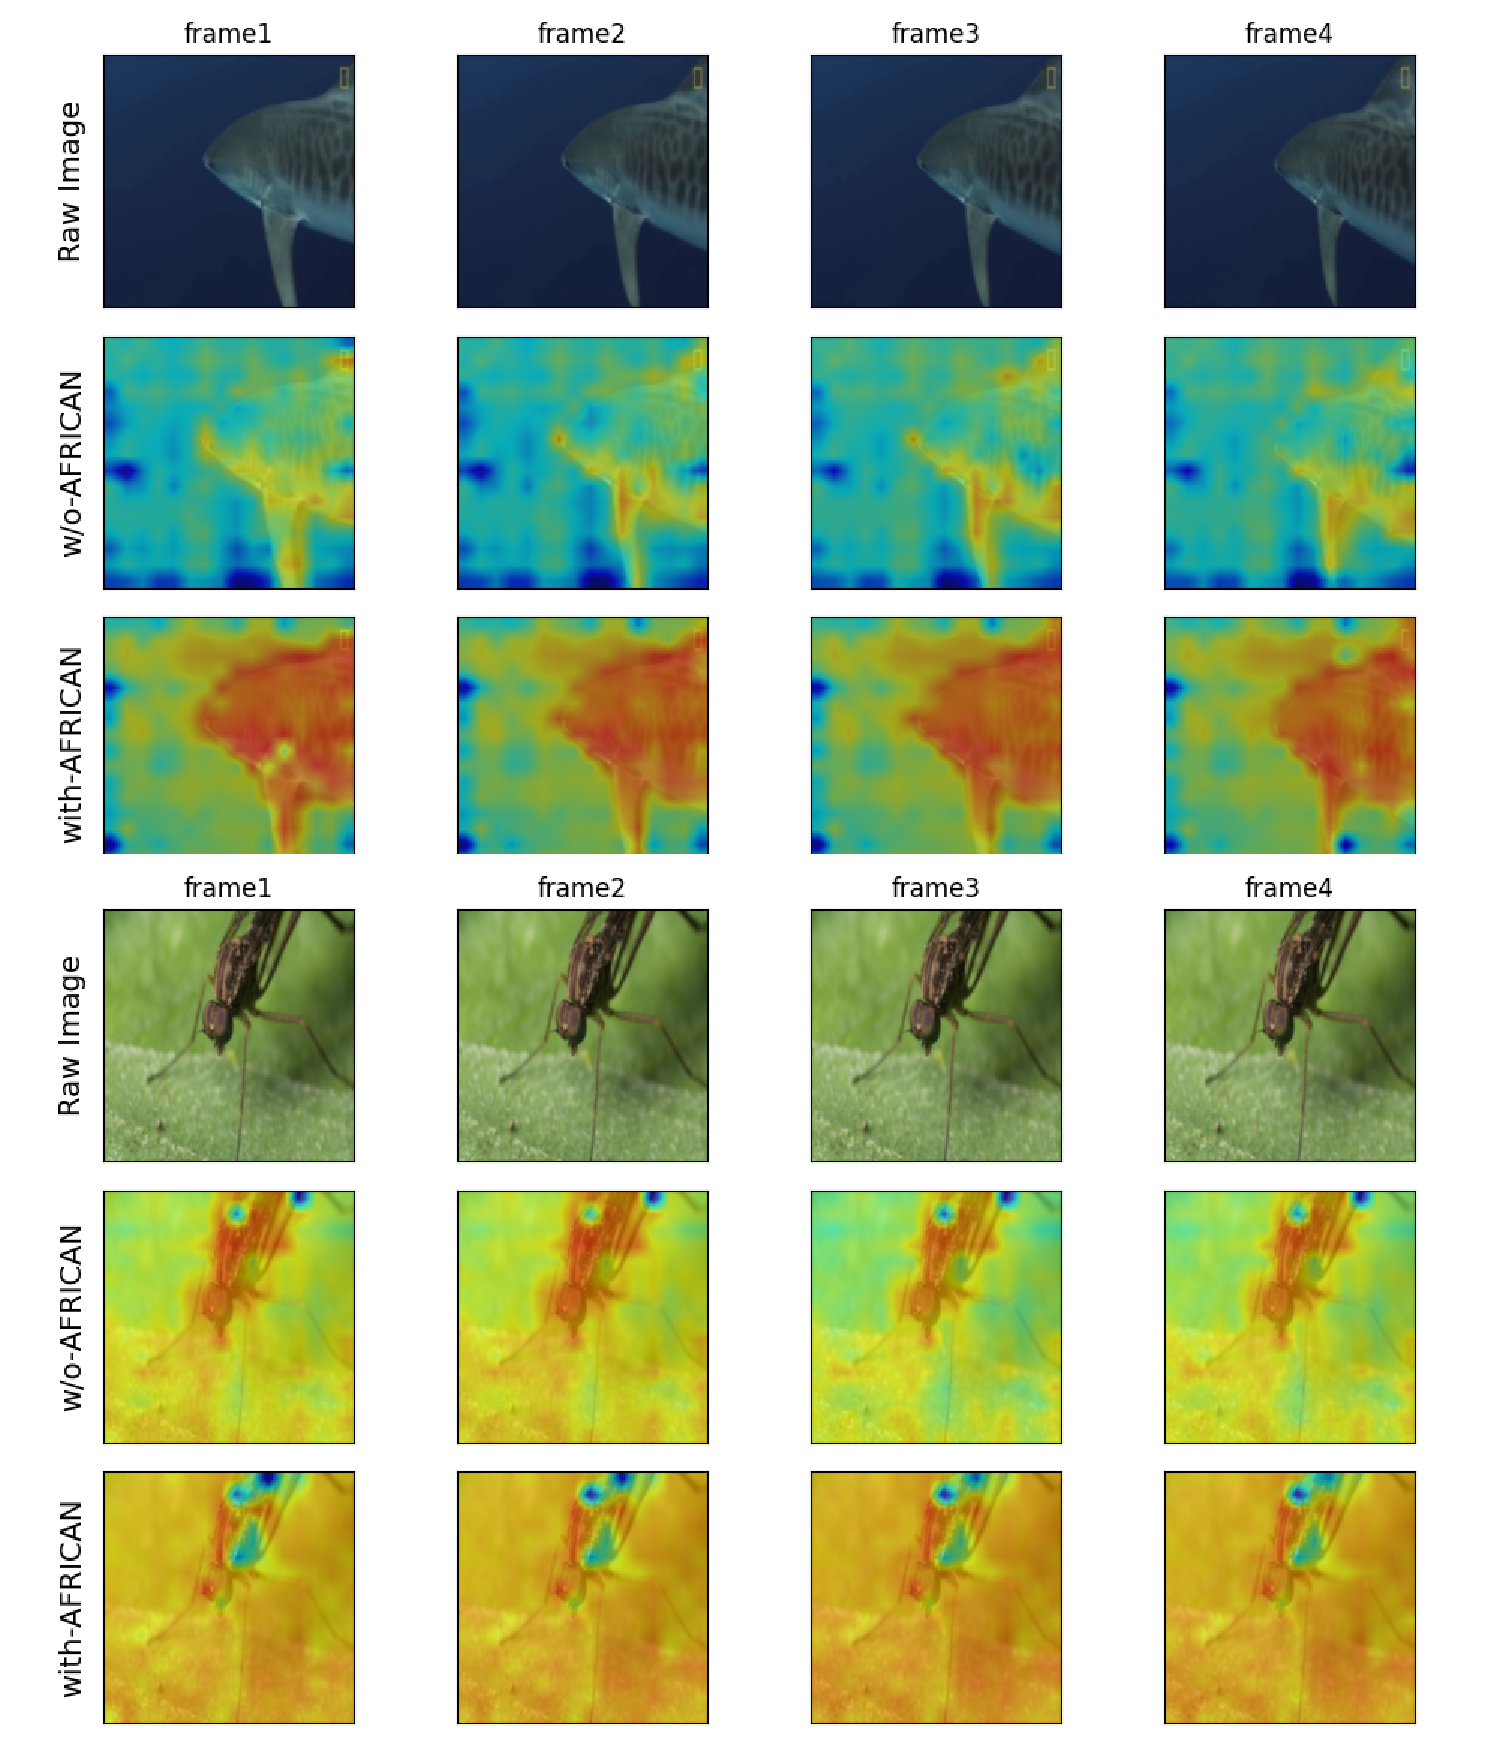
\includegraphics[width=1.0\textwidth]{assets/charts/4_5_AttentionMaps_1}
    \caption[Attention Map 1]{The attention map for three videos. The first row is the input video, the second row is the attention map of w/o-AFRICAN, and the third row is the attention map of with-AFRICAN.}
    \label{fig:attnmap1}
\end{figure}

\begin{figure}[ht]
    \centering
    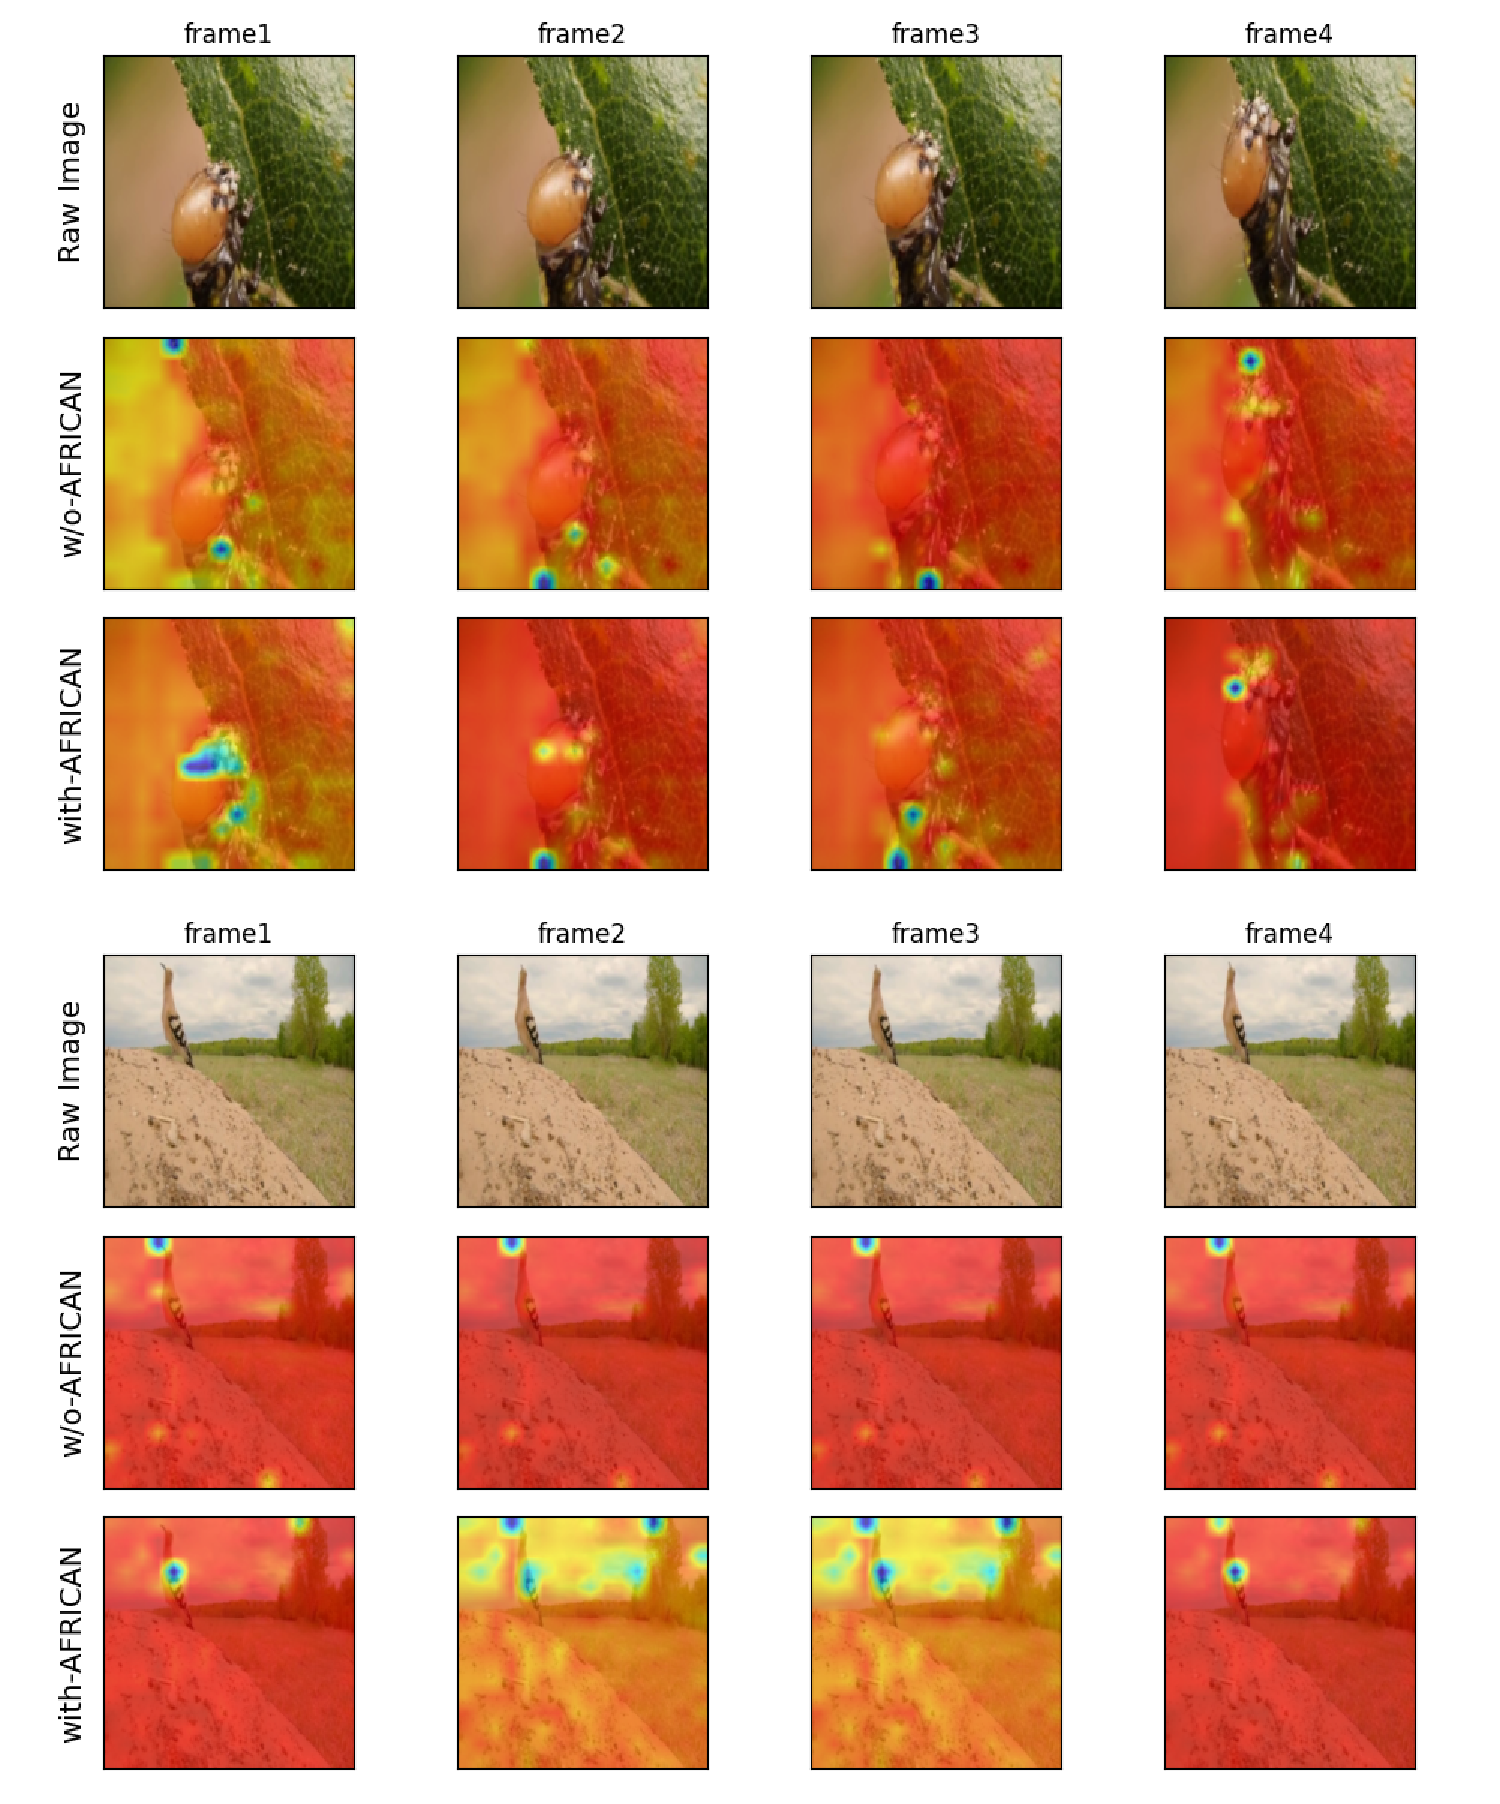
\includegraphics[width=1.0\textwidth]{assets/charts/4_5_AttentionMaps_2}
    \caption[Attention Map 1]{The same with Figure \ref{fig:attnmap1} for another three videos.}
    \label{fig:attnmap2}
\end{figure}







\subsection{Action Recognition Stage}
The AFRICAN model for action recognition, denoted as AFRICAN-AR, the structure is illustrated in Figure \ref{fig:modelstructaf_ar}, which is trained with a Focal Loss and adamw optimizer, using a learning rate of 0.00015 on a single A100 GPU. Since the video clip module of the InterVideo takes longer to converge, as illustrated in Figure \ref{fig:tp_backbone} where the IC model does not improve after Epoch 40, the models are all trained for 40 epochs in this experiment. The mAP is also used as the evaluation metric in this task.

The results for action recognition at Epoch 40 are presented in Table \ref{tab:allresults40}, and the results at the best epoch are shown in Table \ref{tab:allresultsbest}. With the stream of AFRICAN pretrained weights, the AFRICAN-AR are able to outperform the other models in all measured aspects at Epoch 40, with an overall mean Average Precision (mAP) of 54.02\%. At the best epoch, the AFRICAN-AR model generally performs best with an overall mAP of 55.08\%, except in the Tail metric, where IC takes the lead with 48.96\%.


\begin{figure}
    \centering
    \begin{adjustwidth}{-0.2\linewidth}{-0.07\linewidth}
    \begin{subfigure}[b]{0.7\textwidth}
        \includegraphics[width=\textwidth]{assets/charts/4_4_finalscore_0_overall.pdf}
        \caption{Subfigure 1}
        \label{fig:subfig1}
    \end{subfigure}
    \begin{subfigure}[b]{0.7\textwidth}
        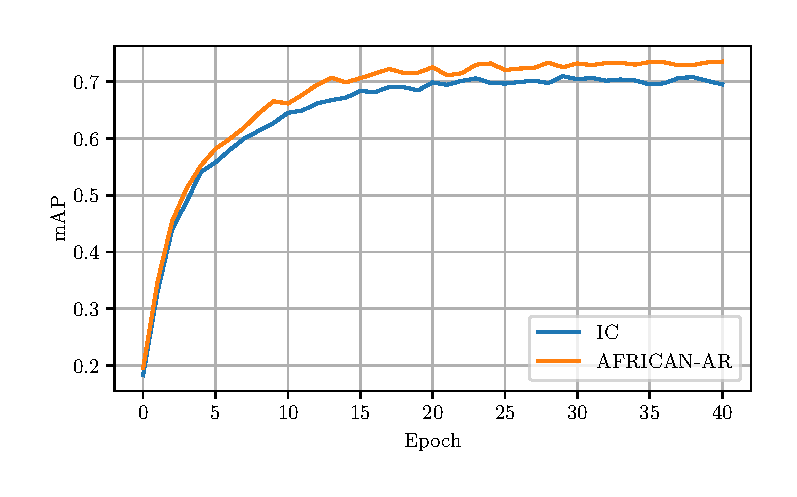
\includegraphics[width=\textwidth]{assets/charts/4_4_finalscore_1_head.pdf}
        \caption{Subfigure 2}
        \label{fig:subfig2}
    \end{subfigure}

    \vspace{10pt} % Adjust the spacing as needed

    \begin{subfigure}[b]{0.7\textwidth}
        \includegraphics[width=\textwidth]{assets/charts/4_4_finalscore_0_overall.pdf}
        \caption{Subfigure 3}
        \label{fig:subfig3}
    \end{subfigure}
    \begin{subfigure}[b]{0.7\textwidth}
        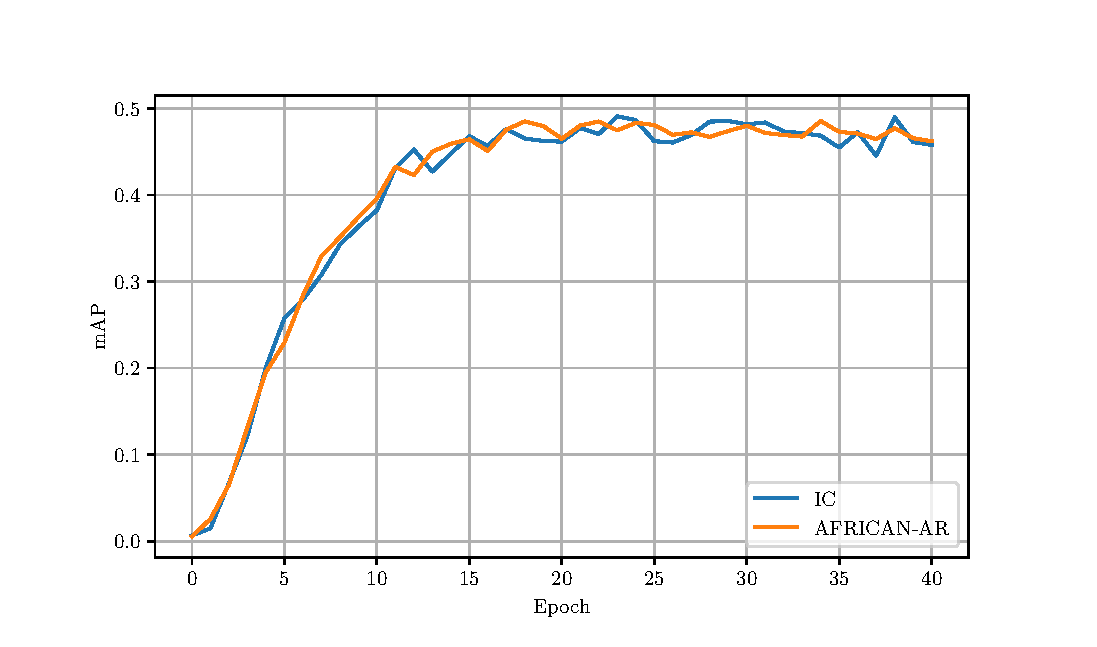
\includegraphics[width=\textwidth]{assets/charts/4_4_finalscore_3_tail.pdf}
        \caption{Subfigure 4}
        \label{fig:subfig4}
    \end{subfigure}
    
    \caption{Main figure caption}
    \label{fig:main}
    
\end{adjustwidth}
\end{figure}


% \begin{figure}[htbp]
%     \centering
%     \subfigure[]{\includegraphics[width=0.4\linewidth]{assets/charts/4_4_finalscore_0_overall.pdf}}
    
%     \subfigure[Caption for Subfigure 2]{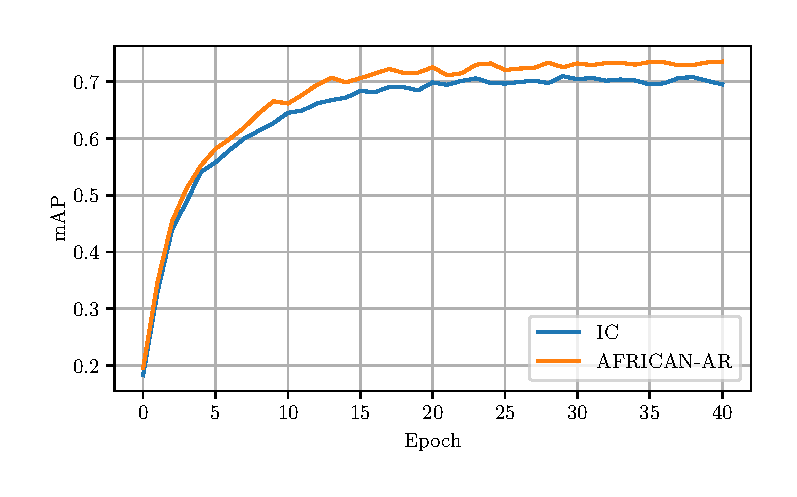
\includegraphics[width=0.4\linewidth]{assets/charts/4_4_finalscore_1_head.pdf}} \\
    
%     \subfigure[Caption for Subfigure 3]{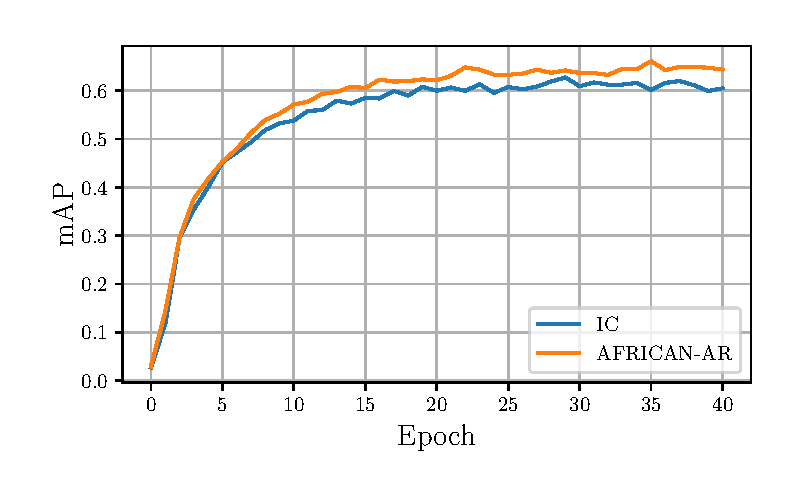
\includegraphics[width=0.4\linewidth]{assets/charts/4_4_finalscore_2_middle.pdf}}
    
%     \subfigure[Caption for Subfigure 4]{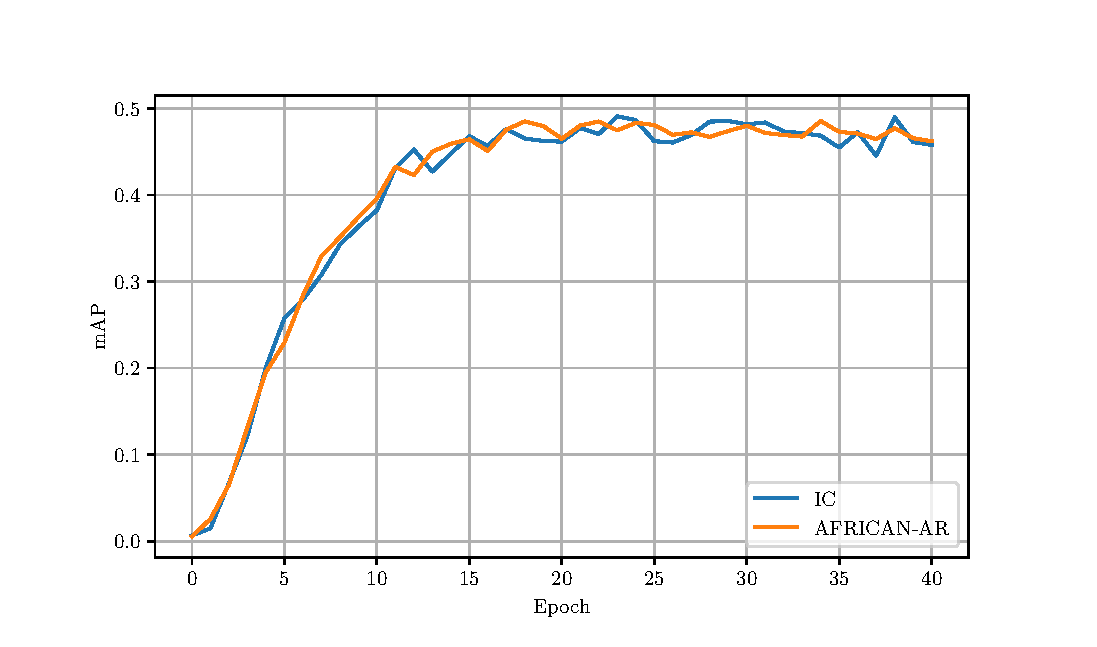
\includegraphics[width=0.4\linewidth]{assets/charts/4_4_finalscore_3_tail.pdf}}
    
%     \caption{The Performance of IC and AFRICAN-AR on each Epoch for Different Segments}
%     \label{fig:trainingprocessfinal}
% \end{figure}


% \begin{figure}
%     \centering

%     \begin{adjustwidth}{-0.15\linewidth}{-0.15\linewidth}
%         \begin{subfigure}{85pt}
%             \includegraphics[scale=0.85]{4_4_finalscore_0_overall.pdf} % a figure 85pt wide
%             \caption{One}
%         \end{subfigure}
%         \begin{subfigure}{85pt}
%             \includegraphics[scale=0.85]{4_4_finalscore_0_overall.pdf} % 
%             \caption{Two}
%         \end{subfigure}
        
%         % \ffigbox[\FBwidth]{\caption{Overall Performancet}\label{subfig:tpf1}}{\includegraphics[width=1\linewidth]{assets/charts/4_4_finalscore_0_overall.pdf}}
%         % \ffigbox[\FBwidth]{\caption{Head Segment Performance}\label{subfig:tpf2}}{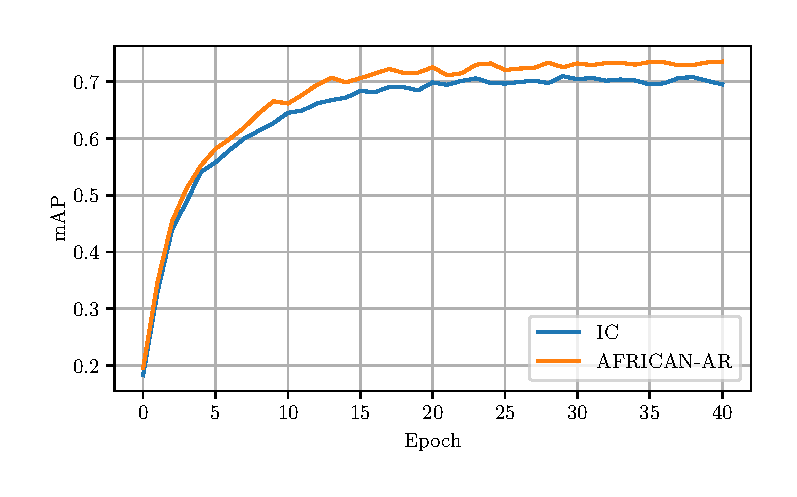
\includegraphics[width=1\linewidth]{assets/charts/4_4_finalscore_1_head.pdf}}
%         % \vspace{-5pt}
%     \end{adjustwidth}
%     \caption{overview: reconstruction (a) and label-mixing~(b).}
%     \label{fig:method}
        
% \end{figure}


% \begin{figure}[htbp]
%     \centering
%     \begin{floatrow}
%         \ffigbox[\FBwidth]{\caption{Overall Performancet}\label{subfig:tpf1}}{\includegraphics[width=1\linewidth]{assets/charts/4_4_finalscore_0_overall.pdf}}
%         \ffigbox[\FBwidth]{\caption{Head Segment Performance}\label{subfig:tpf2}}{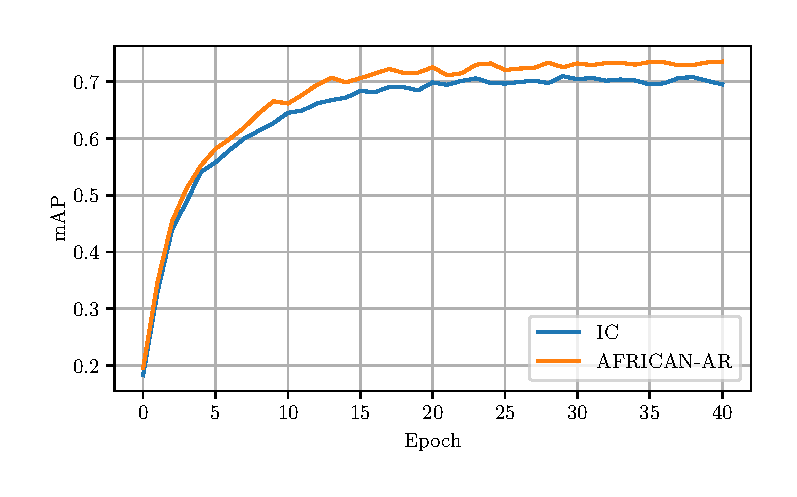
\includegraphics[width=1\linewidth]{assets/charts/4_4_finalscore_1_head.pdf}}
%     \end{floatrow}
        
%     \begin{floatrow}
%         \ffigbox[\FBwidth]{\caption{Middle Segment Performance}\label{subfig:tpf3}}{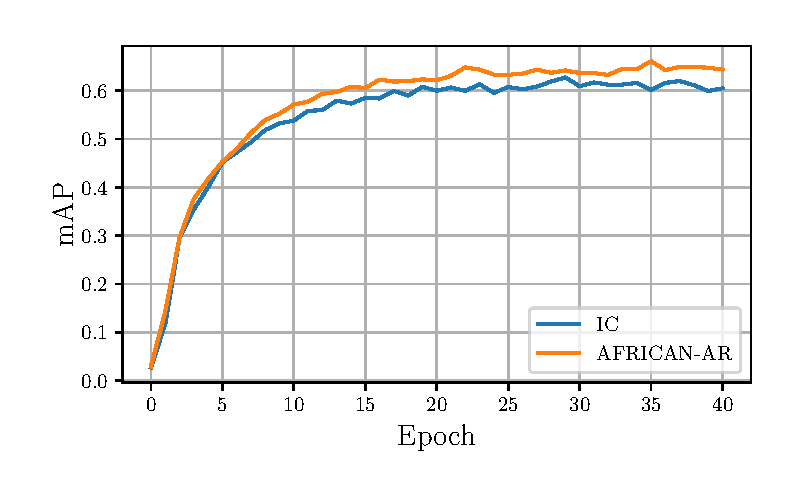
\includegraphics[width=1\linewidth]{assets/charts/4_4_finalscore_2_middle.pdf}}
%         \ffigbox[\FBwidth]{\caption{Tail Segment Performance}\label{subfig:tpf4}}{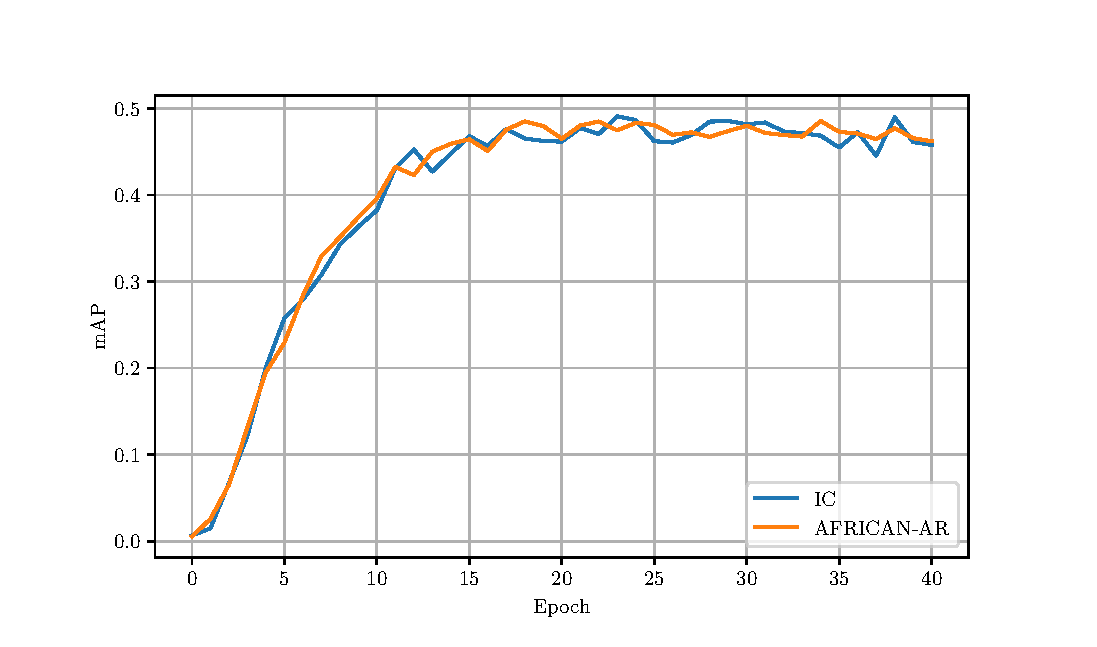
\includegraphics[width=1\linewidth]{assets/charts/4_4_finalscore_3_tail.pdf}}
%     \end{floatrow}
%     \caption[The Performance of IC and AFRICAN-AR on each Epoch for Different Segments]{This figure illustrated The Performance of IC and AFRICAN-AR on each Epoch for Different Segments}
%     \label{fig:trainingprocessfinal}
% \end{figure}


\begin{table}[ht]
    \centering
    \caption{Results of action recognition (Epoch 40)}
    \label{tab:allresults40}
    \begin{tabular}{lllll}
        \toprule
        \multirow{2}{*}{Models} & \multicolumn{4}{c}{mAP} \\
        \cmidrule{2-5} 
        {} & Overall & Head  & Middle & Tail \\
        \midrule
        CARe          & 30.55   & 63.33 & 38.62 & 25.09 \\
        IC            & 52.33   & 69.53 & 60.52 & 45.79 \\        
        AFRICAN-AR    & \textbf{54.02} & \textbf{73.54} & \textbf{64.38} & \textbf{46.21} \\
        \bottomrule
    \end{tabular}
\end{table}

\begin{table}[ht]
    \centering
    \caption{Results of action recognition (Best Epoch)}
    \label{tab:allresultsbest}
    \begin{tabular}{lllll}
        \toprule
        \multirow{2}{*}{Models} & \multicolumn{4}{c}{mAP} \\
        \cmidrule{2-5} 
        {} & Overall & Head  & Middle & Tail \\
        \midrule
        CARe        & 30.55   & 63.33 & 38.62  & 25.09 \\
        IC          & 54.67   & 71.72 & 63.31 & \textbf{48.96} \\
        AFRICAN     & \textbf{55.08} & \textbf{74.16} & \textbf{65.60} & 47.75 \\
        \bottomrule
    \end{tabular}
\end{table}






% % Need ICs1_B
% % Need ICAFs1_B
% % Need ICs1loh B (failed)
% % Need ICs1loh F
% % Need VCs1dd_bs008 F
% % Need VCs1dd_bs032 F
% % Need VCs1_B no text embedding proj


% TODO
% 0. evaluate on the best score
% 1. Add VC vs. IC Section of Ablation Study (Further training 2 epochs for VCdd)
% 2. Update Table for Backbone Selection (wait ICs1_B)
% 3. Update Table For AFRICAN-AR (wait ICAFs1_B)
% 4. (Time Permmited) Add FocalLoss of IC Section Ablation Study
% 4. (Time Permmited) Add batch size section of Ablation Study (VCs1dd_bs008_B and VCs1dd_bs008_B)



\chapter{Discussion}

  \section{Why Does ImageCLIP perform better than VideoCLIP?}
\label{sec:discussion_vc}
\subsection{Domain Adaptation Gap}
VideoCLIP is pretrained on the Kinetics-400 dataset \parencite{kay2017kinetics}, which is a human action dataset, while ImageCLIP is pretrained on a combination of web-crawled and commonly used pre-existing image datasets. As suggested in \parencite{farahani2021brief}, the gap between the animal and human domains may lead to poor performance.

\subsection{Need for More Learnable Weights}
With the Animal Kingdom dataset containing more than 50 hours of animal video clips, it may require more trainable weights to achieve a better fit. To test the effect of different sizes of trainable weights, the following two settings are experimented with to add trainable weights:

\begin{enumerate}
    \item \textbf{VC\_AT}: The VC\_Proj model adds a 12-layer transformer, which is the same as the ImageClip settings in Figure \ref{fig:modelstructure_ic}. Rather than pooling all outputs of ViT's last layer, the embeddings of patches in the same frame are pooled together to obtain the frame-based embedding, which is used as input for the 12-layer transformer.
    \item \textbf{VC\_DF}: This setting is the same as the VC\_Proj model but with two more learnable layers. The Uniformer V2 model, which is the structure used by Invernvideo's video CLIP module, enhances the cross-frame relationship on the final 4 layers of ViT. There are two mechanisms to achieve this, Deep Position Embedding (DPE), a series of 3D CNN layers, and Feed Forward Network (FFN), the attention mechanism on the cls token with two linear layers. These two layers are learnable in this setting.
\end{enumerate}

Table \ref{tab:ablation_vc} and Figure \ref{fig:ablation_vc} show the results of the models with different learnable weights and the performance on each epoch. As illustrated in the figure, it is clear that the VC\_AT model is able to improve the VC\_Proj model to get closer to IC, proving that more learnable weights are indeed helpful for better fitting. Taking advantage of the well-designed mechanism of Uniformer V2, the VC\_DF model is able to achieve a higher score (55.98 mAP) than the IC model (54.36) as demonstrated in the table. 

\begin{table}[ht]
    \centering
    \caption[Training Results for Models with Different Learnable Weights] {This table illustrates the training results for models with different learnable weights. \textbf{VC\_Vision} is VideoCLIP with vision layers learnable, as illustrated in Figure \ref{fig:modelstructure_vc} with a learnable video encoder. \textbf{VC\_Proj} is VideoCLIP with only projection layers learnable, as illustrated in Figure \ref{fig:modelstructure_vc} with a frozen video encoder. \textbf{IC} is ImageCLIP trained on post-transformer layers, as illustrated in Figure \ref{fig:modelstructure_ic} with a frozen image encoder. \textbf{VC\_AT} is the VC\_Proj model that adds a 12-layer transformer. \textbf{VC\_DF}: is the same as the VC\_Proj model but with two more learnable layers.}
    \label{tab:ablation_vc}
    \begin{tabular}{lllll}
        \toprule
        \multirow{2}{*}{Models} & Accuracy \\
        \cmidrule{2-2} 
        {} &  Best Epoch \\
        \midrule
        VC\_Vision & 25.74 \\
        VC\_Proj   & 48.56 \\
        IC         & 54.36 \\
        VC\_AT     & 52.79 \\
        VC\_DF     & 55.98 \\
        \bottomrule
    \end{tabular}
\end{table}

\begin{figure}[ht]
    \centering
    \resizebox{0.8\textwidth}{!}{%% Creator: Matplotlib, PGF backend
%%
%% To include the figure in your LaTeX document, write
%%   \input{<filename>.pgf}
%%
%% Make sure the required packages are loaded in your preamble
%%   \usepackage{pgf}
%%
%% and, on pdftex
%%   \usepackage[utf8]{inputenc}\DeclareUnicodeCharacter{2212}{-}
%%
%% or, on luatex and xetex
%%   \usepackage{unicode-math}
%%
%% Figures using additional raster images can only be included by \input if
%% they are in the same directory as the main LaTeX file. For loading figures
%% from other directories you can use the `import` package
%%   \usepackage{import}
%%
%% and then include the figures with
%%   \import{<path to file>}{<filename>.pgf}
%%
%% Matplotlib used the following preamble
%%
\begingroup%
\makeatletter%
\begin{pgfpicture}%
\pgfpathrectangle{\pgfpointorigin}{\pgfqpoint{7.000000in}{4.000000in}}%
\pgfusepath{use as bounding box, clip}%
\begin{pgfscope}%
\pgfsetbuttcap%
\pgfsetmiterjoin%
\definecolor{currentfill}{rgb}{1.000000,1.000000,1.000000}%
\pgfsetfillcolor{currentfill}%
\pgfsetlinewidth{0.000000pt}%
\definecolor{currentstroke}{rgb}{1.000000,1.000000,1.000000}%
\pgfsetstrokecolor{currentstroke}%
\pgfsetdash{}{0pt}%
\pgfpathmoveto{\pgfqpoint{0.000000in}{0.000000in}}%
\pgfpathlineto{\pgfqpoint{7.000000in}{0.000000in}}%
\pgfpathlineto{\pgfqpoint{7.000000in}{4.000000in}}%
\pgfpathlineto{\pgfqpoint{0.000000in}{4.000000in}}%
\pgfpathclose%
\pgfusepath{fill}%
\end{pgfscope}%
\begin{pgfscope}%
\pgfsetbuttcap%
\pgfsetmiterjoin%
\definecolor{currentfill}{rgb}{1.000000,1.000000,1.000000}%
\pgfsetfillcolor{currentfill}%
\pgfsetlinewidth{0.000000pt}%
\definecolor{currentstroke}{rgb}{0.000000,0.000000,0.000000}%
\pgfsetstrokecolor{currentstroke}%
\pgfsetstrokeopacity{0.000000}%
\pgfsetdash{}{0pt}%
\pgfpathmoveto{\pgfqpoint{0.875000in}{0.440000in}}%
\pgfpathlineto{\pgfqpoint{6.300000in}{0.440000in}}%
\pgfpathlineto{\pgfqpoint{6.300000in}{3.520000in}}%
\pgfpathlineto{\pgfqpoint{0.875000in}{3.520000in}}%
\pgfpathclose%
\pgfusepath{fill}%
\end{pgfscope}%
\begin{pgfscope}%
\pgfpathrectangle{\pgfqpoint{0.875000in}{0.440000in}}{\pgfqpoint{5.425000in}{3.080000in}}%
\pgfusepath{clip}%
\pgfsetrectcap%
\pgfsetroundjoin%
\pgfsetlinewidth{0.803000pt}%
\definecolor{currentstroke}{rgb}{0.690196,0.690196,0.690196}%
\pgfsetstrokecolor{currentstroke}%
\pgfsetdash{}{0pt}%
\pgfpathmoveto{\pgfqpoint{1.121591in}{0.440000in}}%
\pgfpathlineto{\pgfqpoint{1.121591in}{3.520000in}}%
\pgfusepath{stroke}%
\end{pgfscope}%
\begin{pgfscope}%
\pgfsetbuttcap%
\pgfsetroundjoin%
\definecolor{currentfill}{rgb}{0.000000,0.000000,0.000000}%
\pgfsetfillcolor{currentfill}%
\pgfsetlinewidth{0.803000pt}%
\definecolor{currentstroke}{rgb}{0.000000,0.000000,0.000000}%
\pgfsetstrokecolor{currentstroke}%
\pgfsetdash{}{0pt}%
\pgfsys@defobject{currentmarker}{\pgfqpoint{0.000000in}{-0.048611in}}{\pgfqpoint{0.000000in}{0.000000in}}{%
\pgfpathmoveto{\pgfqpoint{0.000000in}{0.000000in}}%
\pgfpathlineto{\pgfqpoint{0.000000in}{-0.048611in}}%
\pgfusepath{stroke,fill}%
}%
\begin{pgfscope}%
\pgfsys@transformshift{1.121591in}{0.440000in}%
\pgfsys@useobject{currentmarker}{}%
\end{pgfscope}%
\end{pgfscope}%
\begin{pgfscope}%
\definecolor{textcolor}{rgb}{0.000000,0.000000,0.000000}%
\pgfsetstrokecolor{textcolor}%
\pgfsetfillcolor{textcolor}%
\pgftext[x=1.121591in,y=0.342778in,,top]{\color{textcolor}\rmfamily\fontsize{10.000000}{12.000000}\selectfont \(\displaystyle {0}\)}%
\end{pgfscope}%
\begin{pgfscope}%
\pgfpathrectangle{\pgfqpoint{0.875000in}{0.440000in}}{\pgfqpoint{5.425000in}{3.080000in}}%
\pgfusepath{clip}%
\pgfsetrectcap%
\pgfsetroundjoin%
\pgfsetlinewidth{0.803000pt}%
\definecolor{currentstroke}{rgb}{0.690196,0.690196,0.690196}%
\pgfsetstrokecolor{currentstroke}%
\pgfsetdash{}{0pt}%
\pgfpathmoveto{\pgfqpoint{2.242459in}{0.440000in}}%
\pgfpathlineto{\pgfqpoint{2.242459in}{3.520000in}}%
\pgfusepath{stroke}%
\end{pgfscope}%
\begin{pgfscope}%
\pgfsetbuttcap%
\pgfsetroundjoin%
\definecolor{currentfill}{rgb}{0.000000,0.000000,0.000000}%
\pgfsetfillcolor{currentfill}%
\pgfsetlinewidth{0.803000pt}%
\definecolor{currentstroke}{rgb}{0.000000,0.000000,0.000000}%
\pgfsetstrokecolor{currentstroke}%
\pgfsetdash{}{0pt}%
\pgfsys@defobject{currentmarker}{\pgfqpoint{0.000000in}{-0.048611in}}{\pgfqpoint{0.000000in}{0.000000in}}{%
\pgfpathmoveto{\pgfqpoint{0.000000in}{0.000000in}}%
\pgfpathlineto{\pgfqpoint{0.000000in}{-0.048611in}}%
\pgfusepath{stroke,fill}%
}%
\begin{pgfscope}%
\pgfsys@transformshift{2.242459in}{0.440000in}%
\pgfsys@useobject{currentmarker}{}%
\end{pgfscope}%
\end{pgfscope}%
\begin{pgfscope}%
\definecolor{textcolor}{rgb}{0.000000,0.000000,0.000000}%
\pgfsetstrokecolor{textcolor}%
\pgfsetfillcolor{textcolor}%
\pgftext[x=2.242459in,y=0.342778in,,top]{\color{textcolor}\rmfamily\fontsize{10.000000}{12.000000}\selectfont \(\displaystyle {10}\)}%
\end{pgfscope}%
\begin{pgfscope}%
\pgfpathrectangle{\pgfqpoint{0.875000in}{0.440000in}}{\pgfqpoint{5.425000in}{3.080000in}}%
\pgfusepath{clip}%
\pgfsetrectcap%
\pgfsetroundjoin%
\pgfsetlinewidth{0.803000pt}%
\definecolor{currentstroke}{rgb}{0.690196,0.690196,0.690196}%
\pgfsetstrokecolor{currentstroke}%
\pgfsetdash{}{0pt}%
\pgfpathmoveto{\pgfqpoint{3.363326in}{0.440000in}}%
\pgfpathlineto{\pgfqpoint{3.363326in}{3.520000in}}%
\pgfusepath{stroke}%
\end{pgfscope}%
\begin{pgfscope}%
\pgfsetbuttcap%
\pgfsetroundjoin%
\definecolor{currentfill}{rgb}{0.000000,0.000000,0.000000}%
\pgfsetfillcolor{currentfill}%
\pgfsetlinewidth{0.803000pt}%
\definecolor{currentstroke}{rgb}{0.000000,0.000000,0.000000}%
\pgfsetstrokecolor{currentstroke}%
\pgfsetdash{}{0pt}%
\pgfsys@defobject{currentmarker}{\pgfqpoint{0.000000in}{-0.048611in}}{\pgfqpoint{0.000000in}{0.000000in}}{%
\pgfpathmoveto{\pgfqpoint{0.000000in}{0.000000in}}%
\pgfpathlineto{\pgfqpoint{0.000000in}{-0.048611in}}%
\pgfusepath{stroke,fill}%
}%
\begin{pgfscope}%
\pgfsys@transformshift{3.363326in}{0.440000in}%
\pgfsys@useobject{currentmarker}{}%
\end{pgfscope}%
\end{pgfscope}%
\begin{pgfscope}%
\definecolor{textcolor}{rgb}{0.000000,0.000000,0.000000}%
\pgfsetstrokecolor{textcolor}%
\pgfsetfillcolor{textcolor}%
\pgftext[x=3.363326in,y=0.342778in,,top]{\color{textcolor}\rmfamily\fontsize{10.000000}{12.000000}\selectfont \(\displaystyle {20}\)}%
\end{pgfscope}%
\begin{pgfscope}%
\pgfpathrectangle{\pgfqpoint{0.875000in}{0.440000in}}{\pgfqpoint{5.425000in}{3.080000in}}%
\pgfusepath{clip}%
\pgfsetrectcap%
\pgfsetroundjoin%
\pgfsetlinewidth{0.803000pt}%
\definecolor{currentstroke}{rgb}{0.690196,0.690196,0.690196}%
\pgfsetstrokecolor{currentstroke}%
\pgfsetdash{}{0pt}%
\pgfpathmoveto{\pgfqpoint{4.484194in}{0.440000in}}%
\pgfpathlineto{\pgfqpoint{4.484194in}{3.520000in}}%
\pgfusepath{stroke}%
\end{pgfscope}%
\begin{pgfscope}%
\pgfsetbuttcap%
\pgfsetroundjoin%
\definecolor{currentfill}{rgb}{0.000000,0.000000,0.000000}%
\pgfsetfillcolor{currentfill}%
\pgfsetlinewidth{0.803000pt}%
\definecolor{currentstroke}{rgb}{0.000000,0.000000,0.000000}%
\pgfsetstrokecolor{currentstroke}%
\pgfsetdash{}{0pt}%
\pgfsys@defobject{currentmarker}{\pgfqpoint{0.000000in}{-0.048611in}}{\pgfqpoint{0.000000in}{0.000000in}}{%
\pgfpathmoveto{\pgfqpoint{0.000000in}{0.000000in}}%
\pgfpathlineto{\pgfqpoint{0.000000in}{-0.048611in}}%
\pgfusepath{stroke,fill}%
}%
\begin{pgfscope}%
\pgfsys@transformshift{4.484194in}{0.440000in}%
\pgfsys@useobject{currentmarker}{}%
\end{pgfscope}%
\end{pgfscope}%
\begin{pgfscope}%
\definecolor{textcolor}{rgb}{0.000000,0.000000,0.000000}%
\pgfsetstrokecolor{textcolor}%
\pgfsetfillcolor{textcolor}%
\pgftext[x=4.484194in,y=0.342778in,,top]{\color{textcolor}\rmfamily\fontsize{10.000000}{12.000000}\selectfont \(\displaystyle {30}\)}%
\end{pgfscope}%
\begin{pgfscope}%
\pgfpathrectangle{\pgfqpoint{0.875000in}{0.440000in}}{\pgfqpoint{5.425000in}{3.080000in}}%
\pgfusepath{clip}%
\pgfsetrectcap%
\pgfsetroundjoin%
\pgfsetlinewidth{0.803000pt}%
\definecolor{currentstroke}{rgb}{0.690196,0.690196,0.690196}%
\pgfsetstrokecolor{currentstroke}%
\pgfsetdash{}{0pt}%
\pgfpathmoveto{\pgfqpoint{5.605062in}{0.440000in}}%
\pgfpathlineto{\pgfqpoint{5.605062in}{3.520000in}}%
\pgfusepath{stroke}%
\end{pgfscope}%
\begin{pgfscope}%
\pgfsetbuttcap%
\pgfsetroundjoin%
\definecolor{currentfill}{rgb}{0.000000,0.000000,0.000000}%
\pgfsetfillcolor{currentfill}%
\pgfsetlinewidth{0.803000pt}%
\definecolor{currentstroke}{rgb}{0.000000,0.000000,0.000000}%
\pgfsetstrokecolor{currentstroke}%
\pgfsetdash{}{0pt}%
\pgfsys@defobject{currentmarker}{\pgfqpoint{0.000000in}{-0.048611in}}{\pgfqpoint{0.000000in}{0.000000in}}{%
\pgfpathmoveto{\pgfqpoint{0.000000in}{0.000000in}}%
\pgfpathlineto{\pgfqpoint{0.000000in}{-0.048611in}}%
\pgfusepath{stroke,fill}%
}%
\begin{pgfscope}%
\pgfsys@transformshift{5.605062in}{0.440000in}%
\pgfsys@useobject{currentmarker}{}%
\end{pgfscope}%
\end{pgfscope}%
\begin{pgfscope}%
\definecolor{textcolor}{rgb}{0.000000,0.000000,0.000000}%
\pgfsetstrokecolor{textcolor}%
\pgfsetfillcolor{textcolor}%
\pgftext[x=5.605062in,y=0.342778in,,top]{\color{textcolor}\rmfamily\fontsize{10.000000}{12.000000}\selectfont \(\displaystyle {40}\)}%
\end{pgfscope}%
\begin{pgfscope}%
\definecolor{textcolor}{rgb}{0.000000,0.000000,0.000000}%
\pgfsetstrokecolor{textcolor}%
\pgfsetfillcolor{textcolor}%
\pgftext[x=3.587500in,y=0.163766in,,top]{\color{textcolor}\rmfamily\fontsize{10.000000}{12.000000}\selectfont Epoch}%
\end{pgfscope}%
\begin{pgfscope}%
\pgfpathrectangle{\pgfqpoint{0.875000in}{0.440000in}}{\pgfqpoint{5.425000in}{3.080000in}}%
\pgfusepath{clip}%
\pgfsetrectcap%
\pgfsetroundjoin%
\pgfsetlinewidth{0.803000pt}%
\definecolor{currentstroke}{rgb}{0.690196,0.690196,0.690196}%
\pgfsetstrokecolor{currentstroke}%
\pgfsetdash{}{0pt}%
\pgfpathmoveto{\pgfqpoint{0.875000in}{0.952019in}}%
\pgfpathlineto{\pgfqpoint{6.300000in}{0.952019in}}%
\pgfusepath{stroke}%
\end{pgfscope}%
\begin{pgfscope}%
\pgfsetbuttcap%
\pgfsetroundjoin%
\definecolor{currentfill}{rgb}{0.000000,0.000000,0.000000}%
\pgfsetfillcolor{currentfill}%
\pgfsetlinewidth{0.803000pt}%
\definecolor{currentstroke}{rgb}{0.000000,0.000000,0.000000}%
\pgfsetstrokecolor{currentstroke}%
\pgfsetdash{}{0pt}%
\pgfsys@defobject{currentmarker}{\pgfqpoint{-0.048611in}{0.000000in}}{\pgfqpoint{0.000000in}{0.000000in}}{%
\pgfpathmoveto{\pgfqpoint{0.000000in}{0.000000in}}%
\pgfpathlineto{\pgfqpoint{-0.048611in}{0.000000in}}%
\pgfusepath{stroke,fill}%
}%
\begin{pgfscope}%
\pgfsys@transformshift{0.875000in}{0.952019in}%
\pgfsys@useobject{currentmarker}{}%
\end{pgfscope}%
\end{pgfscope}%
\begin{pgfscope}%
\definecolor{textcolor}{rgb}{0.000000,0.000000,0.000000}%
\pgfsetstrokecolor{textcolor}%
\pgfsetfillcolor{textcolor}%
\pgftext[x=0.600308in, y=0.903794in, left, base]{\color{textcolor}\rmfamily\fontsize{10.000000}{12.000000}\selectfont \(\displaystyle {0.1}\)}%
\end{pgfscope}%
\begin{pgfscope}%
\pgfpathrectangle{\pgfqpoint{0.875000in}{0.440000in}}{\pgfqpoint{5.425000in}{3.080000in}}%
\pgfusepath{clip}%
\pgfsetrectcap%
\pgfsetroundjoin%
\pgfsetlinewidth{0.803000pt}%
\definecolor{currentstroke}{rgb}{0.690196,0.690196,0.690196}%
\pgfsetstrokecolor{currentstroke}%
\pgfsetdash{}{0pt}%
\pgfpathmoveto{\pgfqpoint{0.875000in}{1.480017in}}%
\pgfpathlineto{\pgfqpoint{6.300000in}{1.480017in}}%
\pgfusepath{stroke}%
\end{pgfscope}%
\begin{pgfscope}%
\pgfsetbuttcap%
\pgfsetroundjoin%
\definecolor{currentfill}{rgb}{0.000000,0.000000,0.000000}%
\pgfsetfillcolor{currentfill}%
\pgfsetlinewidth{0.803000pt}%
\definecolor{currentstroke}{rgb}{0.000000,0.000000,0.000000}%
\pgfsetstrokecolor{currentstroke}%
\pgfsetdash{}{0pt}%
\pgfsys@defobject{currentmarker}{\pgfqpoint{-0.048611in}{0.000000in}}{\pgfqpoint{0.000000in}{0.000000in}}{%
\pgfpathmoveto{\pgfqpoint{0.000000in}{0.000000in}}%
\pgfpathlineto{\pgfqpoint{-0.048611in}{0.000000in}}%
\pgfusepath{stroke,fill}%
}%
\begin{pgfscope}%
\pgfsys@transformshift{0.875000in}{1.480017in}%
\pgfsys@useobject{currentmarker}{}%
\end{pgfscope}%
\end{pgfscope}%
\begin{pgfscope}%
\definecolor{textcolor}{rgb}{0.000000,0.000000,0.000000}%
\pgfsetstrokecolor{textcolor}%
\pgfsetfillcolor{textcolor}%
\pgftext[x=0.600308in, y=1.431792in, left, base]{\color{textcolor}\rmfamily\fontsize{10.000000}{12.000000}\selectfont \(\displaystyle {0.2}\)}%
\end{pgfscope}%
\begin{pgfscope}%
\pgfpathrectangle{\pgfqpoint{0.875000in}{0.440000in}}{\pgfqpoint{5.425000in}{3.080000in}}%
\pgfusepath{clip}%
\pgfsetrectcap%
\pgfsetroundjoin%
\pgfsetlinewidth{0.803000pt}%
\definecolor{currentstroke}{rgb}{0.690196,0.690196,0.690196}%
\pgfsetstrokecolor{currentstroke}%
\pgfsetdash{}{0pt}%
\pgfpathmoveto{\pgfqpoint{0.875000in}{2.008016in}}%
\pgfpathlineto{\pgfqpoint{6.300000in}{2.008016in}}%
\pgfusepath{stroke}%
\end{pgfscope}%
\begin{pgfscope}%
\pgfsetbuttcap%
\pgfsetroundjoin%
\definecolor{currentfill}{rgb}{0.000000,0.000000,0.000000}%
\pgfsetfillcolor{currentfill}%
\pgfsetlinewidth{0.803000pt}%
\definecolor{currentstroke}{rgb}{0.000000,0.000000,0.000000}%
\pgfsetstrokecolor{currentstroke}%
\pgfsetdash{}{0pt}%
\pgfsys@defobject{currentmarker}{\pgfqpoint{-0.048611in}{0.000000in}}{\pgfqpoint{0.000000in}{0.000000in}}{%
\pgfpathmoveto{\pgfqpoint{0.000000in}{0.000000in}}%
\pgfpathlineto{\pgfqpoint{-0.048611in}{0.000000in}}%
\pgfusepath{stroke,fill}%
}%
\begin{pgfscope}%
\pgfsys@transformshift{0.875000in}{2.008016in}%
\pgfsys@useobject{currentmarker}{}%
\end{pgfscope}%
\end{pgfscope}%
\begin{pgfscope}%
\definecolor{textcolor}{rgb}{0.000000,0.000000,0.000000}%
\pgfsetstrokecolor{textcolor}%
\pgfsetfillcolor{textcolor}%
\pgftext[x=0.600308in, y=1.959791in, left, base]{\color{textcolor}\rmfamily\fontsize{10.000000}{12.000000}\selectfont \(\displaystyle {0.3}\)}%
\end{pgfscope}%
\begin{pgfscope}%
\pgfpathrectangle{\pgfqpoint{0.875000in}{0.440000in}}{\pgfqpoint{5.425000in}{3.080000in}}%
\pgfusepath{clip}%
\pgfsetrectcap%
\pgfsetroundjoin%
\pgfsetlinewidth{0.803000pt}%
\definecolor{currentstroke}{rgb}{0.690196,0.690196,0.690196}%
\pgfsetstrokecolor{currentstroke}%
\pgfsetdash{}{0pt}%
\pgfpathmoveto{\pgfqpoint{0.875000in}{2.536014in}}%
\pgfpathlineto{\pgfqpoint{6.300000in}{2.536014in}}%
\pgfusepath{stroke}%
\end{pgfscope}%
\begin{pgfscope}%
\pgfsetbuttcap%
\pgfsetroundjoin%
\definecolor{currentfill}{rgb}{0.000000,0.000000,0.000000}%
\pgfsetfillcolor{currentfill}%
\pgfsetlinewidth{0.803000pt}%
\definecolor{currentstroke}{rgb}{0.000000,0.000000,0.000000}%
\pgfsetstrokecolor{currentstroke}%
\pgfsetdash{}{0pt}%
\pgfsys@defobject{currentmarker}{\pgfqpoint{-0.048611in}{0.000000in}}{\pgfqpoint{0.000000in}{0.000000in}}{%
\pgfpathmoveto{\pgfqpoint{0.000000in}{0.000000in}}%
\pgfpathlineto{\pgfqpoint{-0.048611in}{0.000000in}}%
\pgfusepath{stroke,fill}%
}%
\begin{pgfscope}%
\pgfsys@transformshift{0.875000in}{2.536014in}%
\pgfsys@useobject{currentmarker}{}%
\end{pgfscope}%
\end{pgfscope}%
\begin{pgfscope}%
\definecolor{textcolor}{rgb}{0.000000,0.000000,0.000000}%
\pgfsetstrokecolor{textcolor}%
\pgfsetfillcolor{textcolor}%
\pgftext[x=0.600308in, y=2.487789in, left, base]{\color{textcolor}\rmfamily\fontsize{10.000000}{12.000000}\selectfont \(\displaystyle {0.4}\)}%
\end{pgfscope}%
\begin{pgfscope}%
\pgfpathrectangle{\pgfqpoint{0.875000in}{0.440000in}}{\pgfqpoint{5.425000in}{3.080000in}}%
\pgfusepath{clip}%
\pgfsetrectcap%
\pgfsetroundjoin%
\pgfsetlinewidth{0.803000pt}%
\definecolor{currentstroke}{rgb}{0.690196,0.690196,0.690196}%
\pgfsetstrokecolor{currentstroke}%
\pgfsetdash{}{0pt}%
\pgfpathmoveto{\pgfqpoint{0.875000in}{3.064013in}}%
\pgfpathlineto{\pgfqpoint{6.300000in}{3.064013in}}%
\pgfusepath{stroke}%
\end{pgfscope}%
\begin{pgfscope}%
\pgfsetbuttcap%
\pgfsetroundjoin%
\definecolor{currentfill}{rgb}{0.000000,0.000000,0.000000}%
\pgfsetfillcolor{currentfill}%
\pgfsetlinewidth{0.803000pt}%
\definecolor{currentstroke}{rgb}{0.000000,0.000000,0.000000}%
\pgfsetstrokecolor{currentstroke}%
\pgfsetdash{}{0pt}%
\pgfsys@defobject{currentmarker}{\pgfqpoint{-0.048611in}{0.000000in}}{\pgfqpoint{0.000000in}{0.000000in}}{%
\pgfpathmoveto{\pgfqpoint{0.000000in}{0.000000in}}%
\pgfpathlineto{\pgfqpoint{-0.048611in}{0.000000in}}%
\pgfusepath{stroke,fill}%
}%
\begin{pgfscope}%
\pgfsys@transformshift{0.875000in}{3.064013in}%
\pgfsys@useobject{currentmarker}{}%
\end{pgfscope}%
\end{pgfscope}%
\begin{pgfscope}%
\definecolor{textcolor}{rgb}{0.000000,0.000000,0.000000}%
\pgfsetstrokecolor{textcolor}%
\pgfsetfillcolor{textcolor}%
\pgftext[x=0.600308in, y=3.015788in, left, base]{\color{textcolor}\rmfamily\fontsize{10.000000}{12.000000}\selectfont \(\displaystyle {0.5}\)}%
\end{pgfscope}%
\begin{pgfscope}%
\definecolor{textcolor}{rgb}{0.000000,0.000000,0.000000}%
\pgfsetstrokecolor{textcolor}%
\pgfsetfillcolor{textcolor}%
\pgftext[x=0.544752in,y=1.980000in,,bottom,rotate=90.000000]{\color{textcolor}\rmfamily\fontsize{10.000000}{12.000000}\selectfont mAP}%
\end{pgfscope}%
\begin{pgfscope}%
\pgfpathrectangle{\pgfqpoint{0.875000in}{0.440000in}}{\pgfqpoint{5.425000in}{3.080000in}}%
\pgfusepath{clip}%
\pgfsetrectcap%
\pgfsetroundjoin%
\pgfsetlinewidth{1.505625pt}%
\definecolor{currentstroke}{rgb}{0.121569,0.466667,0.705882}%
\pgfsetstrokecolor{currentstroke}%
\pgfsetdash{}{0pt}%
\pgfpathmoveto{\pgfqpoint{1.121591in}{0.794420in}}%
\pgfpathlineto{\pgfqpoint{1.233678in}{1.027653in}}%
\pgfpathlineto{\pgfqpoint{1.345764in}{1.091314in}}%
\pgfpathlineto{\pgfqpoint{1.457851in}{1.196405in}}%
\pgfpathlineto{\pgfqpoint{1.569938in}{1.238666in}}%
\pgfpathlineto{\pgfqpoint{1.682025in}{1.309640in}}%
\pgfpathlineto{\pgfqpoint{1.794112in}{1.325704in}}%
\pgfpathlineto{\pgfqpoint{1.906198in}{1.370793in}}%
\pgfpathlineto{\pgfqpoint{2.018285in}{1.408075in}}%
\pgfpathlineto{\pgfqpoint{2.130372in}{1.434875in}}%
\pgfpathlineto{\pgfqpoint{2.242459in}{1.405676in}}%
\pgfpathlineto{\pgfqpoint{2.354545in}{1.457186in}}%
\pgfpathlineto{\pgfqpoint{2.466632in}{1.469218in}}%
\pgfpathlineto{\pgfqpoint{2.578719in}{1.452434in}}%
\pgfpathlineto{\pgfqpoint{2.690806in}{1.504031in}}%
\pgfpathlineto{\pgfqpoint{2.802893in}{1.495361in}}%
\pgfpathlineto{\pgfqpoint{2.914979in}{1.594839in}}%
\pgfpathlineto{\pgfqpoint{3.027066in}{1.567836in}}%
\pgfpathlineto{\pgfqpoint{3.139153in}{1.592304in}}%
\pgfpathlineto{\pgfqpoint{3.251240in}{1.619042in}}%
\pgfpathlineto{\pgfqpoint{3.363326in}{1.579572in}}%
\pgfpathlineto{\pgfqpoint{3.475413in}{1.618569in}}%
\pgfpathlineto{\pgfqpoint{3.587500in}{1.621920in}}%
\pgfpathlineto{\pgfqpoint{3.699587in}{1.669461in}}%
\pgfpathlineto{\pgfqpoint{3.811674in}{1.678185in}}%
\pgfpathlineto{\pgfqpoint{3.923760in}{1.625954in}}%
\pgfpathlineto{\pgfqpoint{4.035847in}{1.627907in}}%
\pgfpathlineto{\pgfqpoint{4.147934in}{1.660259in}}%
\pgfpathlineto{\pgfqpoint{4.260021in}{1.701571in}}%
\pgfpathlineto{\pgfqpoint{4.372107in}{1.611735in}}%
\pgfpathlineto{\pgfqpoint{4.484194in}{1.620648in}}%
\pgfpathlineto{\pgfqpoint{4.596281in}{1.703444in}}%
\pgfpathlineto{\pgfqpoint{4.708368in}{1.748424in}}%
\pgfpathlineto{\pgfqpoint{4.820455in}{1.653477in}}%
\pgfpathlineto{\pgfqpoint{4.932541in}{1.659607in}}%
\pgfpathlineto{\pgfqpoint{5.044628in}{1.731411in}}%
\pgfpathlineto{\pgfqpoint{5.156715in}{1.758110in}}%
\pgfpathlineto{\pgfqpoint{5.268802in}{1.674757in}}%
\pgfpathlineto{\pgfqpoint{5.380888in}{1.675480in}}%
\pgfpathlineto{\pgfqpoint{5.492975in}{1.740303in}}%
\pgfpathlineto{\pgfqpoint{5.605062in}{1.773579in}}%
\pgfpathlineto{\pgfqpoint{5.717149in}{1.705983in}}%
\pgfpathlineto{\pgfqpoint{5.829236in}{1.778915in}}%
\pgfpathlineto{\pgfqpoint{5.941322in}{1.783211in}}%
\pgfpathlineto{\pgfqpoint{6.053409in}{1.722756in}}%
\pgfusepath{stroke}%
\end{pgfscope}%
\begin{pgfscope}%
\pgfpathrectangle{\pgfqpoint{0.875000in}{0.440000in}}{\pgfqpoint{5.425000in}{3.080000in}}%
\pgfusepath{clip}%
\pgfsetrectcap%
\pgfsetroundjoin%
\pgfsetlinewidth{1.505625pt}%
\definecolor{currentstroke}{rgb}{1.000000,0.498039,0.054902}%
\pgfsetstrokecolor{currentstroke}%
\pgfsetdash{}{0pt}%
\pgfpathmoveto{\pgfqpoint{1.121591in}{0.721853in}}%
\pgfpathlineto{\pgfqpoint{1.233678in}{0.989522in}}%
\pgfpathlineto{\pgfqpoint{1.345764in}{1.316511in}}%
\pgfpathlineto{\pgfqpoint{1.457851in}{1.566373in}}%
\pgfpathlineto{\pgfqpoint{1.569938in}{1.767084in}}%
\pgfpathlineto{\pgfqpoint{1.682025in}{1.922472in}}%
\pgfpathlineto{\pgfqpoint{1.794112in}{2.059887in}}%
\pgfpathlineto{\pgfqpoint{1.906198in}{2.159993in}}%
\pgfpathlineto{\pgfqpoint{2.018285in}{2.159395in}}%
\pgfpathlineto{\pgfqpoint{2.130372in}{2.240519in}}%
\pgfpathlineto{\pgfqpoint{2.242459in}{2.283632in}}%
\pgfpathlineto{\pgfqpoint{2.354545in}{2.310369in}}%
\pgfpathlineto{\pgfqpoint{2.466632in}{2.339204in}}%
\pgfpathlineto{\pgfqpoint{2.578719in}{2.423511in}}%
\pgfpathlineto{\pgfqpoint{2.690806in}{2.470443in}}%
\pgfpathlineto{\pgfqpoint{2.802893in}{2.517835in}}%
\pgfpathlineto{\pgfqpoint{2.914979in}{2.587466in}}%
\pgfpathlineto{\pgfqpoint{3.027066in}{2.608468in}}%
\pgfpathlineto{\pgfqpoint{3.139153in}{2.632554in}}%
\pgfpathlineto{\pgfqpoint{3.251240in}{2.658438in}}%
\pgfpathlineto{\pgfqpoint{3.363326in}{2.727905in}}%
\pgfpathlineto{\pgfqpoint{3.475413in}{2.722807in}}%
\pgfpathlineto{\pgfqpoint{3.587500in}{2.705966in}}%
\pgfpathlineto{\pgfqpoint{3.699587in}{2.769312in}}%
\pgfpathlineto{\pgfqpoint{3.811674in}{2.777067in}}%
\pgfpathlineto{\pgfqpoint{3.923760in}{2.795322in}}%
\pgfpathlineto{\pgfqpoint{4.035847in}{2.845021in}}%
\pgfpathlineto{\pgfqpoint{4.147934in}{2.830722in}}%
\pgfpathlineto{\pgfqpoint{4.260021in}{2.821705in}}%
\pgfpathlineto{\pgfqpoint{4.372107in}{2.858022in}}%
\pgfpathlineto{\pgfqpoint{4.484194in}{2.900390in}}%
\pgfpathlineto{\pgfqpoint{4.596281in}{2.900669in}}%
\pgfpathlineto{\pgfqpoint{4.708368in}{2.903477in}}%
\pgfpathlineto{\pgfqpoint{4.820455in}{2.899729in}}%
\pgfpathlineto{\pgfqpoint{4.932541in}{2.889217in}}%
\pgfpathlineto{\pgfqpoint{5.044628in}{2.902871in}}%
\pgfpathlineto{\pgfqpoint{5.156715in}{2.921001in}}%
\pgfpathlineto{\pgfqpoint{5.268802in}{2.954180in}}%
\pgfpathlineto{\pgfqpoint{5.380888in}{2.941926in}}%
\pgfpathlineto{\pgfqpoint{5.492975in}{2.936950in}}%
\pgfpathlineto{\pgfqpoint{5.605062in}{2.926707in}}%
\pgfpathlineto{\pgfqpoint{5.717149in}{2.925351in}}%
\pgfpathlineto{\pgfqpoint{5.829236in}{2.935878in}}%
\pgfpathlineto{\pgfqpoint{5.941322in}{2.964802in}}%
\pgfpathlineto{\pgfqpoint{6.053409in}{2.977233in}}%
\pgfusepath{stroke}%
\end{pgfscope}%
\begin{pgfscope}%
\pgfpathrectangle{\pgfqpoint{0.875000in}{0.440000in}}{\pgfqpoint{5.425000in}{3.080000in}}%
\pgfusepath{clip}%
\pgfsetrectcap%
\pgfsetroundjoin%
\pgfsetlinewidth{1.505625pt}%
\definecolor{currentstroke}{rgb}{0.172549,0.627451,0.172549}%
\pgfsetstrokecolor{currentstroke}%
\pgfsetdash{}{0pt}%
\pgfpathmoveto{\pgfqpoint{1.121591in}{0.591695in}}%
\pgfpathlineto{\pgfqpoint{1.233678in}{0.882775in}}%
\pgfpathlineto{\pgfqpoint{1.345764in}{1.313313in}}%
\pgfpathlineto{\pgfqpoint{1.457851in}{1.606833in}}%
\pgfpathlineto{\pgfqpoint{1.569938in}{1.852613in}}%
\pgfpathlineto{\pgfqpoint{1.682025in}{2.044065in}}%
\pgfpathlineto{\pgfqpoint{1.794112in}{2.170504in}}%
\pgfpathlineto{\pgfqpoint{1.906198in}{2.344349in}}%
\pgfpathlineto{\pgfqpoint{2.018285in}{2.457863in}}%
\pgfpathlineto{\pgfqpoint{2.130372in}{2.628144in}}%
\pgfpathlineto{\pgfqpoint{2.242459in}{2.739498in}}%
\pgfpathlineto{\pgfqpoint{2.354545in}{2.762542in}}%
\pgfpathlineto{\pgfqpoint{2.466632in}{2.961023in}}%
\pgfpathlineto{\pgfqpoint{2.578719in}{2.916196in}}%
\pgfpathlineto{\pgfqpoint{2.690806in}{2.942286in}}%
\pgfpathlineto{\pgfqpoint{2.802893in}{3.076958in}}%
\pgfpathlineto{\pgfqpoint{2.914979in}{3.095885in}}%
\pgfpathlineto{\pgfqpoint{3.027066in}{3.155078in}}%
\pgfpathlineto{\pgfqpoint{3.139153in}{3.180644in}}%
\pgfpathlineto{\pgfqpoint{3.251240in}{3.162332in}}%
\pgfpathlineto{\pgfqpoint{3.363326in}{3.151018in}}%
\pgfpathlineto{\pgfqpoint{3.475413in}{3.159255in}}%
\pgfpathlineto{\pgfqpoint{3.587500in}{3.161949in}}%
\pgfpathlineto{\pgfqpoint{3.699587in}{3.120742in}}%
\pgfpathlineto{\pgfqpoint{3.811674in}{3.226537in}}%
\pgfpathlineto{\pgfqpoint{3.923760in}{3.160760in}}%
\pgfpathlineto{\pgfqpoint{4.035847in}{3.178010in}}%
\pgfpathlineto{\pgfqpoint{4.147934in}{3.163055in}}%
\pgfpathlineto{\pgfqpoint{4.260021in}{3.130229in}}%
\pgfpathlineto{\pgfqpoint{4.372107in}{3.187088in}}%
\pgfpathlineto{\pgfqpoint{4.484194in}{3.166750in}}%
\pgfpathlineto{\pgfqpoint{4.596281in}{3.252697in}}%
\pgfpathlineto{\pgfqpoint{4.708368in}{3.185257in}}%
\pgfpathlineto{\pgfqpoint{4.820455in}{3.178796in}}%
\pgfpathlineto{\pgfqpoint{4.932541in}{3.215919in}}%
\pgfpathlineto{\pgfqpoint{5.044628in}{3.130265in}}%
\pgfpathlineto{\pgfqpoint{5.156715in}{3.058678in}}%
\pgfpathlineto{\pgfqpoint{5.268802in}{3.175757in}}%
\pgfpathlineto{\pgfqpoint{5.380888in}{3.136306in}}%
\pgfpathlineto{\pgfqpoint{5.492975in}{3.294290in}}%
\pgfpathlineto{\pgfqpoint{5.605062in}{3.272709in}}%
\pgfpathlineto{\pgfqpoint{5.717149in}{3.202851in}}%
\pgfpathlineto{\pgfqpoint{5.829236in}{3.231690in}}%
\pgfpathlineto{\pgfqpoint{5.941322in}{3.224348in}}%
\pgfpathlineto{\pgfqpoint{6.053409in}{3.182074in}}%
\pgfusepath{stroke}%
\end{pgfscope}%
\begin{pgfscope}%
\pgfpathrectangle{\pgfqpoint{0.875000in}{0.440000in}}{\pgfqpoint{5.425000in}{3.080000in}}%
\pgfusepath{clip}%
\pgfsetrectcap%
\pgfsetroundjoin%
\pgfsetlinewidth{1.505625pt}%
\definecolor{currentstroke}{rgb}{0.839216,0.152941,0.156863}%
\pgfsetstrokecolor{currentstroke}%
\pgfsetdash{}{0pt}%
\pgfpathmoveto{\pgfqpoint{1.121591in}{0.580000in}}%
\pgfpathlineto{\pgfqpoint{1.233678in}{0.803507in}}%
\pgfpathlineto{\pgfqpoint{1.345764in}{1.127010in}}%
\pgfpathlineto{\pgfqpoint{1.457851in}{1.353141in}}%
\pgfpathlineto{\pgfqpoint{1.569938in}{1.616298in}}%
\pgfpathlineto{\pgfqpoint{1.682025in}{1.825786in}}%
\pgfpathlineto{\pgfqpoint{1.794112in}{1.995441in}}%
\pgfpathlineto{\pgfqpoint{1.906198in}{2.116216in}}%
\pgfpathlineto{\pgfqpoint{2.018285in}{2.208378in}}%
\pgfpathlineto{\pgfqpoint{2.130372in}{2.295069in}}%
\pgfpathlineto{\pgfqpoint{2.242459in}{2.416954in}}%
\pgfpathlineto{\pgfqpoint{2.354545in}{2.516432in}}%
\pgfpathlineto{\pgfqpoint{2.466632in}{2.596323in}}%
\pgfpathlineto{\pgfqpoint{2.578719in}{2.685392in}}%
\pgfpathlineto{\pgfqpoint{2.690806in}{2.693883in}}%
\pgfpathlineto{\pgfqpoint{2.802893in}{2.670101in}}%
\pgfpathlineto{\pgfqpoint{2.914979in}{2.761856in}}%
\pgfpathlineto{\pgfqpoint{3.027066in}{2.830363in}}%
\pgfpathlineto{\pgfqpoint{3.139153in}{2.915250in}}%
\pgfpathlineto{\pgfqpoint{3.251240in}{2.961761in}}%
\pgfpathlineto{\pgfqpoint{3.363326in}{2.951188in}}%
\pgfpathlineto{\pgfqpoint{3.475413in}{3.021331in}}%
\pgfpathlineto{\pgfqpoint{3.587500in}{2.950606in}}%
\pgfpathlineto{\pgfqpoint{3.699587in}{3.039663in}}%
\pgfpathlineto{\pgfqpoint{3.811674in}{3.044181in}}%
\pgfpathlineto{\pgfqpoint{3.923760in}{3.031809in}}%
\pgfpathlineto{\pgfqpoint{4.035847in}{3.050892in}}%
\pgfpathlineto{\pgfqpoint{4.147934in}{3.167862in}}%
\pgfpathlineto{\pgfqpoint{4.260021in}{3.152225in}}%
\pgfpathlineto{\pgfqpoint{4.372107in}{3.131782in}}%
\pgfpathlineto{\pgfqpoint{4.484194in}{3.125953in}}%
\pgfpathlineto{\pgfqpoint{4.596281in}{3.054681in}}%
\pgfpathlineto{\pgfqpoint{4.708368in}{3.148501in}}%
\pgfpathlineto{\pgfqpoint{4.820455in}{3.078978in}}%
\pgfpathlineto{\pgfqpoint{4.932541in}{3.145105in}}%
\pgfpathlineto{\pgfqpoint{5.044628in}{3.159238in}}%
\pgfpathlineto{\pgfqpoint{5.156715in}{3.133748in}}%
\pgfpathlineto{\pgfqpoint{5.268802in}{3.211372in}}%
\pgfpathlineto{\pgfqpoint{5.380888in}{3.100855in}}%
\pgfpathlineto{\pgfqpoint{5.492975in}{3.118200in}}%
\pgfpathlineto{\pgfqpoint{5.605062in}{3.083581in}}%
\pgfpathlineto{\pgfqpoint{5.717149in}{3.150881in}}%
\pgfpathlineto{\pgfqpoint{5.829236in}{3.143639in}}%
\pgfpathlineto{\pgfqpoint{5.941322in}{3.172443in}}%
\pgfpathlineto{\pgfqpoint{6.053409in}{3.168845in}}%
\pgfusepath{stroke}%
\end{pgfscope}%
\begin{pgfscope}%
\pgfpathrectangle{\pgfqpoint{0.875000in}{0.440000in}}{\pgfqpoint{5.425000in}{3.080000in}}%
\pgfusepath{clip}%
\pgfsetrectcap%
\pgfsetroundjoin%
\pgfsetlinewidth{1.505625pt}%
\definecolor{currentstroke}{rgb}{0.580392,0.403922,0.741176}%
\pgfsetstrokecolor{currentstroke}%
\pgfsetdash{}{0pt}%
\pgfpathmoveto{\pgfqpoint{1.121591in}{0.639769in}}%
\pgfpathlineto{\pgfqpoint{1.233678in}{1.093957in}}%
\pgfpathlineto{\pgfqpoint{1.345764in}{1.656795in}}%
\pgfpathlineto{\pgfqpoint{1.457851in}{2.101539in}}%
\pgfpathlineto{\pgfqpoint{1.569938in}{2.408292in}}%
\pgfpathlineto{\pgfqpoint{1.682025in}{2.573609in}}%
\pgfpathlineto{\pgfqpoint{1.794112in}{2.738487in}}%
\pgfpathlineto{\pgfqpoint{1.906198in}{2.822770in}}%
\pgfpathlineto{\pgfqpoint{2.018285in}{3.026883in}}%
\pgfpathlineto{\pgfqpoint{2.130372in}{3.220540in}}%
\pgfpathlineto{\pgfqpoint{2.242459in}{3.178296in}}%
\pgfpathlineto{\pgfqpoint{2.354545in}{3.195939in}}%
\pgfpathlineto{\pgfqpoint{2.466632in}{3.282921in}}%
\pgfpathlineto{\pgfqpoint{2.578719in}{3.375577in}}%
\pgfpathlineto{\pgfqpoint{2.690806in}{3.305021in}}%
\pgfpathlineto{\pgfqpoint{2.802893in}{3.340196in}}%
\pgfpathlineto{\pgfqpoint{2.914979in}{3.334386in}}%
\pgfpathlineto{\pgfqpoint{3.027066in}{3.279123in}}%
\pgfpathlineto{\pgfqpoint{3.139153in}{3.318571in}}%
\pgfpathlineto{\pgfqpoint{3.251240in}{3.325257in}}%
\pgfpathlineto{\pgfqpoint{3.363326in}{3.358281in}}%
\pgfpathlineto{\pgfqpoint{3.475413in}{3.334700in}}%
\pgfpathlineto{\pgfqpoint{3.587500in}{3.380000in}}%
\pgfpathlineto{\pgfqpoint{3.699587in}{3.305650in}}%
\pgfpathlineto{\pgfqpoint{3.811674in}{3.229410in}}%
\pgfpathlineto{\pgfqpoint{3.923760in}{3.273604in}}%
\pgfpathlineto{\pgfqpoint{4.035847in}{3.293667in}}%
\pgfpathlineto{\pgfqpoint{4.147934in}{3.279072in}}%
\pgfpathlineto{\pgfqpoint{4.260021in}{3.328606in}}%
\pgfpathlineto{\pgfqpoint{4.372107in}{3.321667in}}%
\pgfpathlineto{\pgfqpoint{4.484194in}{3.296235in}}%
\pgfpathlineto{\pgfqpoint{4.596281in}{3.354814in}}%
\pgfpathlineto{\pgfqpoint{4.708368in}{3.219488in}}%
\pgfpathlineto{\pgfqpoint{4.820455in}{3.244387in}}%
\pgfpathlineto{\pgfqpoint{4.932541in}{3.215811in}}%
\pgfpathlineto{\pgfqpoint{5.044628in}{3.360403in}}%
\pgfpathlineto{\pgfqpoint{5.156715in}{3.321280in}}%
\pgfpathlineto{\pgfqpoint{5.268802in}{3.283906in}}%
\pgfpathlineto{\pgfqpoint{5.380888in}{3.299952in}}%
\pgfpathlineto{\pgfqpoint{5.492975in}{3.166286in}}%
\pgfpathlineto{\pgfqpoint{5.605062in}{3.129849in}}%
\pgfpathlineto{\pgfqpoint{5.717149in}{3.152619in}}%
\pgfpathlineto{\pgfqpoint{5.829236in}{3.201982in}}%
\pgfpathlineto{\pgfqpoint{5.941322in}{3.224898in}}%
\pgfpathlineto{\pgfqpoint{6.053409in}{3.266513in}}%
\pgfusepath{stroke}%
\end{pgfscope}%
\begin{pgfscope}%
\pgfsetrectcap%
\pgfsetmiterjoin%
\pgfsetlinewidth{0.803000pt}%
\definecolor{currentstroke}{rgb}{0.000000,0.000000,0.000000}%
\pgfsetstrokecolor{currentstroke}%
\pgfsetdash{}{0pt}%
\pgfpathmoveto{\pgfqpoint{0.875000in}{0.440000in}}%
\pgfpathlineto{\pgfqpoint{0.875000in}{3.520000in}}%
\pgfusepath{stroke}%
\end{pgfscope}%
\begin{pgfscope}%
\pgfsetrectcap%
\pgfsetmiterjoin%
\pgfsetlinewidth{0.803000pt}%
\definecolor{currentstroke}{rgb}{0.000000,0.000000,0.000000}%
\pgfsetstrokecolor{currentstroke}%
\pgfsetdash{}{0pt}%
\pgfpathmoveto{\pgfqpoint{6.300000in}{0.440000in}}%
\pgfpathlineto{\pgfqpoint{6.300000in}{3.520000in}}%
\pgfusepath{stroke}%
\end{pgfscope}%
\begin{pgfscope}%
\pgfsetrectcap%
\pgfsetmiterjoin%
\pgfsetlinewidth{0.803000pt}%
\definecolor{currentstroke}{rgb}{0.000000,0.000000,0.000000}%
\pgfsetstrokecolor{currentstroke}%
\pgfsetdash{}{0pt}%
\pgfpathmoveto{\pgfqpoint{0.875000in}{0.440000in}}%
\pgfpathlineto{\pgfqpoint{6.300000in}{0.440000in}}%
\pgfusepath{stroke}%
\end{pgfscope}%
\begin{pgfscope}%
\pgfsetrectcap%
\pgfsetmiterjoin%
\pgfsetlinewidth{0.803000pt}%
\definecolor{currentstroke}{rgb}{0.000000,0.000000,0.000000}%
\pgfsetstrokecolor{currentstroke}%
\pgfsetdash{}{0pt}%
\pgfpathmoveto{\pgfqpoint{0.875000in}{3.520000in}}%
\pgfpathlineto{\pgfqpoint{6.300000in}{3.520000in}}%
\pgfusepath{stroke}%
\end{pgfscope}%
\begin{pgfscope}%
\pgfsetbuttcap%
\pgfsetmiterjoin%
\definecolor{currentfill}{rgb}{1.000000,1.000000,1.000000}%
\pgfsetfillcolor{currentfill}%
\pgfsetfillopacity{0.800000}%
\pgfsetlinewidth{1.003750pt}%
\definecolor{currentstroke}{rgb}{0.800000,0.800000,0.800000}%
\pgfsetstrokecolor{currentstroke}%
\pgfsetstrokeopacity{0.800000}%
\pgfsetdash{}{0pt}%
\pgfpathmoveto{\pgfqpoint{5.124999in}{0.509444in}}%
\pgfpathlineto{\pgfqpoint{6.202778in}{0.509444in}}%
\pgfpathquadraticcurveto{\pgfqpoint{6.230556in}{0.509444in}}{\pgfqpoint{6.230556in}{0.537222in}}%
\pgfpathlineto{\pgfqpoint{6.230556in}{1.491697in}}%
\pgfpathquadraticcurveto{\pgfqpoint{6.230556in}{1.519475in}}{\pgfqpoint{6.202778in}{1.519475in}}%
\pgfpathlineto{\pgfqpoint{5.124999in}{1.519475in}}%
\pgfpathquadraticcurveto{\pgfqpoint{5.097221in}{1.519475in}}{\pgfqpoint{5.097221in}{1.491697in}}%
\pgfpathlineto{\pgfqpoint{5.097221in}{0.537222in}}%
\pgfpathquadraticcurveto{\pgfqpoint{5.097221in}{0.509444in}}{\pgfqpoint{5.124999in}{0.509444in}}%
\pgfpathclose%
\pgfusepath{stroke,fill}%
\end{pgfscope}%
\begin{pgfscope}%
\pgfsetrectcap%
\pgfsetroundjoin%
\pgfsetlinewidth{1.505625pt}%
\definecolor{currentstroke}{rgb}{0.121569,0.466667,0.705882}%
\pgfsetstrokecolor{currentstroke}%
\pgfsetdash{}{0pt}%
\pgfpathmoveto{\pgfqpoint{5.152777in}{1.415308in}}%
\pgfpathlineto{\pgfqpoint{5.430554in}{1.415308in}}%
\pgfusepath{stroke}%
\end{pgfscope}%
\begin{pgfscope}%
\definecolor{textcolor}{rgb}{0.000000,0.000000,0.000000}%
\pgfsetstrokecolor{textcolor}%
\pgfsetfillcolor{textcolor}%
\pgftext[x=5.541666in,y=1.366697in,left,base]{\color{textcolor}\rmfamily\fontsize{10.000000}{12.000000}\selectfont VC\_Vision}%
\end{pgfscope}%
\begin{pgfscope}%
\pgfsetrectcap%
\pgfsetroundjoin%
\pgfsetlinewidth{1.505625pt}%
\definecolor{currentstroke}{rgb}{1.000000,0.498039,0.054902}%
\pgfsetstrokecolor{currentstroke}%
\pgfsetdash{}{0pt}%
\pgfpathmoveto{\pgfqpoint{5.152777in}{1.221636in}}%
\pgfpathlineto{\pgfqpoint{5.430554in}{1.221636in}}%
\pgfusepath{stroke}%
\end{pgfscope}%
\begin{pgfscope}%
\definecolor{textcolor}{rgb}{0.000000,0.000000,0.000000}%
\pgfsetstrokecolor{textcolor}%
\pgfsetfillcolor{textcolor}%
\pgftext[x=5.541666in,y=1.173024in,left,base]{\color{textcolor}\rmfamily\fontsize{10.000000}{12.000000}\selectfont VC\_Proj}%
\end{pgfscope}%
\begin{pgfscope}%
\pgfsetrectcap%
\pgfsetroundjoin%
\pgfsetlinewidth{1.505625pt}%
\definecolor{currentstroke}{rgb}{0.172549,0.627451,0.172549}%
\pgfsetstrokecolor{currentstroke}%
\pgfsetdash{}{0pt}%
\pgfpathmoveto{\pgfqpoint{5.152777in}{1.027963in}}%
\pgfpathlineto{\pgfqpoint{5.430554in}{1.027963in}}%
\pgfusepath{stroke}%
\end{pgfscope}%
\begin{pgfscope}%
\definecolor{textcolor}{rgb}{0.000000,0.000000,0.000000}%
\pgfsetstrokecolor{textcolor}%
\pgfsetfillcolor{textcolor}%
\pgftext[x=5.541666in,y=0.979352in,left,base]{\color{textcolor}\rmfamily\fontsize{10.000000}{12.000000}\selectfont IC}%
\end{pgfscope}%
\begin{pgfscope}%
\pgfsetrectcap%
\pgfsetroundjoin%
\pgfsetlinewidth{1.505625pt}%
\definecolor{currentstroke}{rgb}{0.839216,0.152941,0.156863}%
\pgfsetstrokecolor{currentstroke}%
\pgfsetdash{}{0pt}%
\pgfpathmoveto{\pgfqpoint{5.152777in}{0.834290in}}%
\pgfpathlineto{\pgfqpoint{5.430554in}{0.834290in}}%
\pgfusepath{stroke}%
\end{pgfscope}%
\begin{pgfscope}%
\definecolor{textcolor}{rgb}{0.000000,0.000000,0.000000}%
\pgfsetstrokecolor{textcolor}%
\pgfsetfillcolor{textcolor}%
\pgftext[x=5.541666in,y=0.785679in,left,base]{\color{textcolor}\rmfamily\fontsize{10.000000}{12.000000}\selectfont VC\_AT}%
\end{pgfscope}%
\begin{pgfscope}%
\pgfsetrectcap%
\pgfsetroundjoin%
\pgfsetlinewidth{1.505625pt}%
\definecolor{currentstroke}{rgb}{0.580392,0.403922,0.741176}%
\pgfsetstrokecolor{currentstroke}%
\pgfsetdash{}{0pt}%
\pgfpathmoveto{\pgfqpoint{5.152777in}{0.640617in}}%
\pgfpathlineto{\pgfqpoint{5.430554in}{0.640617in}}%
\pgfusepath{stroke}%
\end{pgfscope}%
\begin{pgfscope}%
\definecolor{textcolor}{rgb}{0.000000,0.000000,0.000000}%
\pgfsetstrokecolor{textcolor}%
\pgfsetfillcolor{textcolor}%
\pgftext[x=5.541666in,y=0.592006in,left,base]{\color{textcolor}\rmfamily\fontsize{10.000000}{12.000000}\selectfont VC\_DF}%
\end{pgfscope}%
\end{pgfpicture}%
\makeatother%
\endgroup%
}
    \caption[mAP of VC\_Vision, VC\_Proj, IC, VC\_AT, VC\_DF on each Epoch]{This chart illustrates the mAP of VC\_Vision, VC\_Proj, IC, VC\_AT, VC\_DF on each epoch.}
    \label{fig:ablation_vc}
\end{figure}

\section{Why Does MSQNet perform better than AFRICAN?}
\label{sec:discussion_msqnet}

\subsection{Model Structure}
\begin{figure}[ht]
    \centering
    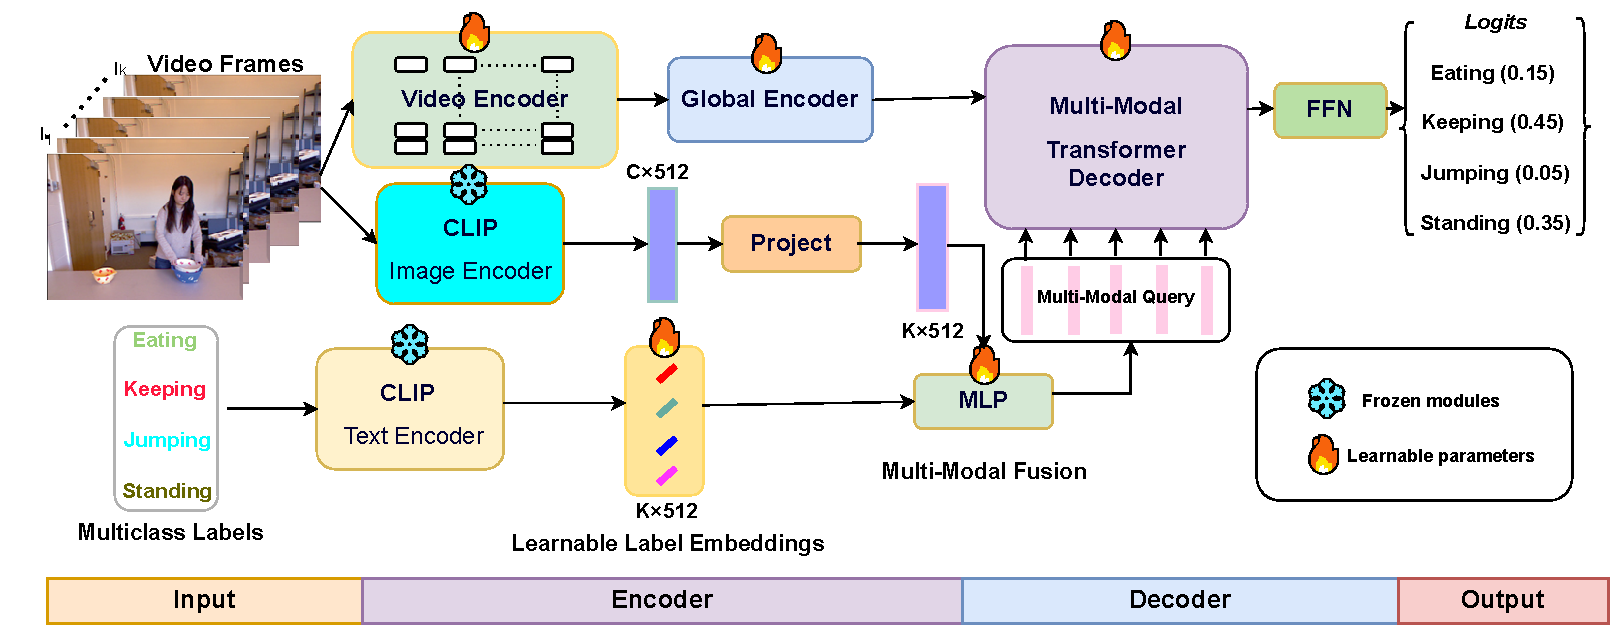
\includegraphics[width=1.0\textwidth]{assets/charts_rw/MSQNet}
    \caption[Model Structure of MSQNet]{Illustration of MSQNet's model structure. Source \parencite{mondal2023msqnet}}
    \label{fig:discussion_msqnet}
\end{figure}

Figure \ref{fig:discussion_msqnet} presents the model structure of MSQNet. The core module of this structure is the Multi-Modal Transformer Decoder (MMTD). The entire structure can be divided into three parts: 

\begin{enumerate}
    \item \textbf{Key and Value of MMTD}: The input video $X \in \mathbf{R}^{N, T, C, H, W}$ is processed by the video encoder, specifically the TimeSformer, where $N$ represents the batch size, $T$ represents the number of frames, and C, H and W represents the channels, width and height of a frame, respectively. By averaging pooling patch embeddings generated by the video encoder within the same frame, frame-level embeddings are obtained. These embeddings are subsequently multiplied by the projection weights $W \in \mathbf{R}^{D \times D}$ to yield the key and value of the MMTD in the shape $(N, D)$. 
    \item \textbf{Query of MMTD}: The video embedding $Q_v \in \mathbf{R}^{N \times D}$ is derived from the average pooling of frame embeddings encoded by the image encoder of CLIP. The learnable class embedding $Q_l \in \mathbf{R}^{K \times D}$ is initialised with the text encoder of CLIP, taking the original label text as input, where $K$ denotes the number of classes. To produce a query $Q \in \mathbf{R}^{K \times D}$, the embeddings $Q_v$ and $Q_l$ are concatenated, resulting in $Q \in \mathbf{R}^{K \times 2D}$, which is then projected using the weight $W \in \mathbf{R}^{2D \times D}$. 
    \item \textbf{operation of MMTD}: Several layers of the cross-attention mechanism are applied to the query, key, and value to produce the embedding for each class $Q^l \in \mathbf{R}^{K \times D}$, where $l \in L$ represents the. This is then followed by an FFN module to produce the class logits.
\end{enumerate}

\subsection{Comparison}
Three key differences exist between AFRICAN and MSQNet: 

\begin{enumerate}
    \item \textbf{Cross-Attention}: The cross-attention mechanism enables the model to compute attention between the label embeddings and frame-level embedding, which is the most meticulously designed mechanism in this structure.
    \item \textbf{Learnable label Embedding}: Unlike AFRICAN, which uses fixed label embedding, MSQNet initialises the learnable label embedding with values produced by the pretrained CLIP model. This allows the model to update the weights of the label embedding to fit better.
    \item \textbf{Fusion of Image and Text Embedding}: Instead of adopting CLIP's similarity calculation method, MSQNet concatenates the text and video embeddings with a projection layer to fuse them together. 
\end{enumerate}

These features make MSQNet more adaptable to fit on a medium-sized dataset. On the contrary, AFRICAN tries to mimic the training scheme to directly calculate the image-text similarity for action recognition. Although this enables the model to update a minimum number of parameters to achieve an acceptable result, it restricts the model's potential to better fit the data. Given that MSQNet was published a month prior to the submission of this dissertation and their code is not yet publicly available, the improvement may be further studied in the future.

\subsection{Implementation}
To better quantify the improvement caused by the three differences mentioned above. I do the following three experiments

\begin{enumerate}
    \item \textbf{}: 
    \item \textbf{}
    \item \textbf{}
    \item \textbf{}
\end{enumerate}




learnable label embedding
LLE
\begin{table}[ht]
    \centering
    \caption[] {}
    \label{tab:ablation_vc}
    \begin{tabular}{lllll}
        \toprule
        \multirow{2}{*}{Models} & Accuracy \\
        \cmidrule{2-2} 
        {} &  Best Epoch \\
        \midrule
        VC\_DF & 25.74 \\
        MSQ_TS_LLE   & 48.56 \\
        MSQ_VC_LLE   & 48.56 \\
        MSQ_TS_LLE         & 54.36 \\
        VC\_AT     & 52.79 \\
        VC\_DF     & 55.98 \\
        \bottomrule
    \end{tabular}
\end{table}



Test Test Test Test Test Test Test Test Test Test Test Test Test Test Test Test Test Test Test Test Test Test Test Test Test Test Test Test Test Test Test Test Test Test Test Test Test Test Test Test Test Test Test Test Test Test Test Test Test Test Test Test Test Test Test Test Test Test Test Test Test Test Test Test.
Test Test Test Test Test Test Test Test Test Test Test Test Test Test Test Test Test Test Test Test Test Test Test Test Test Test Test Test Test Test Test Test Test Test Test Test Test Test Test Test Test Test Test Test Test Test Test Test Test Test Test Test Test Test Test Test Test Test Test Test Test Test Test Test.
Test Test Test Test Test Test Test Test Test Test Test Test Test Test Test Test Test Test Test Test Test Test Test Test Test Test Test Test Test Test Test Test Test Test Test Test Test Test Test Test Test Test Test Test Test Test Test Test Test Test Test Test Test Test Test Test Test Test Test Test Test Test Test Test.
Test Test Test Test Test Test Test Test Test Test Test Test Test Test Test Test Test Test Test Test Test Test Test Test Test Test Test Test Test Test Test Test Test Test Test Test Test Test Test Test Test Test Test Test Test Test Test Test Test Test Test Test Test Test Test Test Test Test Test Test Test Test Test Test.
Test Test Test Test Test Test Test Test Test Test Test Test Test Test Test Test Test Test Test Test Test Test Test Test Test Test Test Test Test Test Test Test Test Test Test Test Test Test Test Test Test Test Test Test Test Test Test Test Test Test Test Test Test Test Test Test Test Test Test Test Test Test Test Test.
Test Test Test Test Test Test Test Test Test Test Test Test Test Test Test Test Test Test Test Test Test Test Test Test Test Test Test Test Test Test Test Test Test Test Test Test Test Test Test Test Test Test Test Test Test Test Test Test Test Test Test Test Test Test Test Test Test Test Test Test Test Test Test Test.
% \subsection{The effect smaller of batch size}
% Owing to the 80 Gb limitation of A100 GPU, I am able to train the fully learnable model, VC\_Vision, with a batch size of 16. To investigate the effect of this, I compare the 


% 0.514509499	0.543613255	0.559846222	0.257423162	0.481209993
% VC_AT	    IC	        VC_dd	    VC2_Vision	VC2_Proj


\chapter{Future Work}

  \section{CLIP with Prompt Engineering}
% \subsection{Impact of Batch Size on Long-Tail Dataset}
% There are very few studies that focus on the impact of batch size on long-tail datasets. Some of my experiments suggest that the learning curves of models with different batch sizes perform differently. In the range of batch sizes from 8 to 128, large batch sizes may lead to better performance. For example, Figure \ref{fig:futurework_bs} shows the VC\_AT with batch sizes of 16 and 128, denoted as VC\_AT\_bs16 and VC\_AT\_bs128. VC\_AT\_bs16 increases rapidly but reaches a lower ceiling, while VC\_AT\_bs128 may perform better in the end.

% \begin{figure}[ht]
%     \centering
%     \resizebox{1.0\textwidth}{!}{%% Creator: Matplotlib, PGF backend
%%
%% To include the figure in your LaTeX document, write
%%   \input{<filename>.pgf}
%%
%% Make sure the required packages are loaded in your preamble
%%   \usepackage{pgf}
%%
%% and, on pdftex
%%   \usepackage[utf8]{inputenc}\DeclareUnicodeCharacter{2212}{-}
%%
%% or, on luatex and xetex
%%   \usepackage{unicode-math}
%%
%% Figures using additional raster images can only be included by \input if
%% they are in the same directory as the main LaTeX file. For loading figures
%% from other directories you can use the `import` package
%%   \usepackage{import}
%%
%% and then include the figures with
%%   \import{<path to file>}{<filename>.pgf}
%%
%% Matplotlib used the following preamble
%%
\begingroup%
\makeatletter%
\begin{pgfpicture}%
\pgfpathrectangle{\pgfpointorigin}{\pgfqpoint{7.000000in}{4.000000in}}%
\pgfusepath{use as bounding box, clip}%
\begin{pgfscope}%
\pgfsetbuttcap%
\pgfsetmiterjoin%
\definecolor{currentfill}{rgb}{1.000000,1.000000,1.000000}%
\pgfsetfillcolor{currentfill}%
\pgfsetlinewidth{0.000000pt}%
\definecolor{currentstroke}{rgb}{1.000000,1.000000,1.000000}%
\pgfsetstrokecolor{currentstroke}%
\pgfsetdash{}{0pt}%
\pgfpathmoveto{\pgfqpoint{0.000000in}{0.000000in}}%
\pgfpathlineto{\pgfqpoint{7.000000in}{0.000000in}}%
\pgfpathlineto{\pgfqpoint{7.000000in}{4.000000in}}%
\pgfpathlineto{\pgfqpoint{0.000000in}{4.000000in}}%
\pgfpathclose%
\pgfusepath{fill}%
\end{pgfscope}%
\begin{pgfscope}%
\pgfsetbuttcap%
\pgfsetmiterjoin%
\definecolor{currentfill}{rgb}{1.000000,1.000000,1.000000}%
\pgfsetfillcolor{currentfill}%
\pgfsetlinewidth{0.000000pt}%
\definecolor{currentstroke}{rgb}{0.000000,0.000000,0.000000}%
\pgfsetstrokecolor{currentstroke}%
\pgfsetstrokeopacity{0.000000}%
\pgfsetdash{}{0pt}%
\pgfpathmoveto{\pgfqpoint{0.875000in}{0.440000in}}%
\pgfpathlineto{\pgfqpoint{6.300000in}{0.440000in}}%
\pgfpathlineto{\pgfqpoint{6.300000in}{3.520000in}}%
\pgfpathlineto{\pgfqpoint{0.875000in}{3.520000in}}%
\pgfpathclose%
\pgfusepath{fill}%
\end{pgfscope}%
\begin{pgfscope}%
\pgfpathrectangle{\pgfqpoint{0.875000in}{0.440000in}}{\pgfqpoint{5.425000in}{3.080000in}}%
\pgfusepath{clip}%
\pgfsetrectcap%
\pgfsetroundjoin%
\pgfsetlinewidth{0.803000pt}%
\definecolor{currentstroke}{rgb}{0.690196,0.690196,0.690196}%
\pgfsetstrokecolor{currentstroke}%
\pgfsetdash{}{0pt}%
\pgfpathmoveto{\pgfqpoint{1.121591in}{0.440000in}}%
\pgfpathlineto{\pgfqpoint{1.121591in}{3.520000in}}%
\pgfusepath{stroke}%
\end{pgfscope}%
\begin{pgfscope}%
\pgfsetbuttcap%
\pgfsetroundjoin%
\definecolor{currentfill}{rgb}{0.000000,0.000000,0.000000}%
\pgfsetfillcolor{currentfill}%
\pgfsetlinewidth{0.803000pt}%
\definecolor{currentstroke}{rgb}{0.000000,0.000000,0.000000}%
\pgfsetstrokecolor{currentstroke}%
\pgfsetdash{}{0pt}%
\pgfsys@defobject{currentmarker}{\pgfqpoint{0.000000in}{-0.048611in}}{\pgfqpoint{0.000000in}{0.000000in}}{%
\pgfpathmoveto{\pgfqpoint{0.000000in}{0.000000in}}%
\pgfpathlineto{\pgfqpoint{0.000000in}{-0.048611in}}%
\pgfusepath{stroke,fill}%
}%
\begin{pgfscope}%
\pgfsys@transformshift{1.121591in}{0.440000in}%
\pgfsys@useobject{currentmarker}{}%
\end{pgfscope}%
\end{pgfscope}%
\begin{pgfscope}%
\definecolor{textcolor}{rgb}{0.000000,0.000000,0.000000}%
\pgfsetstrokecolor{textcolor}%
\pgfsetfillcolor{textcolor}%
\pgftext[x=1.121591in,y=0.342778in,,top]{\color{textcolor}\rmfamily\fontsize{10.000000}{12.000000}\selectfont \(\displaystyle {0}\)}%
\end{pgfscope}%
\begin{pgfscope}%
\pgfpathrectangle{\pgfqpoint{0.875000in}{0.440000in}}{\pgfqpoint{5.425000in}{3.080000in}}%
\pgfusepath{clip}%
\pgfsetrectcap%
\pgfsetroundjoin%
\pgfsetlinewidth{0.803000pt}%
\definecolor{currentstroke}{rgb}{0.690196,0.690196,0.690196}%
\pgfsetstrokecolor{currentstroke}%
\pgfsetdash{}{0pt}%
\pgfpathmoveto{\pgfqpoint{1.738068in}{0.440000in}}%
\pgfpathlineto{\pgfqpoint{1.738068in}{3.520000in}}%
\pgfusepath{stroke}%
\end{pgfscope}%
\begin{pgfscope}%
\pgfsetbuttcap%
\pgfsetroundjoin%
\definecolor{currentfill}{rgb}{0.000000,0.000000,0.000000}%
\pgfsetfillcolor{currentfill}%
\pgfsetlinewidth{0.803000pt}%
\definecolor{currentstroke}{rgb}{0.000000,0.000000,0.000000}%
\pgfsetstrokecolor{currentstroke}%
\pgfsetdash{}{0pt}%
\pgfsys@defobject{currentmarker}{\pgfqpoint{0.000000in}{-0.048611in}}{\pgfqpoint{0.000000in}{0.000000in}}{%
\pgfpathmoveto{\pgfqpoint{0.000000in}{0.000000in}}%
\pgfpathlineto{\pgfqpoint{0.000000in}{-0.048611in}}%
\pgfusepath{stroke,fill}%
}%
\begin{pgfscope}%
\pgfsys@transformshift{1.738068in}{0.440000in}%
\pgfsys@useobject{currentmarker}{}%
\end{pgfscope}%
\end{pgfscope}%
\begin{pgfscope}%
\definecolor{textcolor}{rgb}{0.000000,0.000000,0.000000}%
\pgfsetstrokecolor{textcolor}%
\pgfsetfillcolor{textcolor}%
\pgftext[x=1.738068in,y=0.342778in,,top]{\color{textcolor}\rmfamily\fontsize{10.000000}{12.000000}\selectfont \(\displaystyle {5}\)}%
\end{pgfscope}%
\begin{pgfscope}%
\pgfpathrectangle{\pgfqpoint{0.875000in}{0.440000in}}{\pgfqpoint{5.425000in}{3.080000in}}%
\pgfusepath{clip}%
\pgfsetrectcap%
\pgfsetroundjoin%
\pgfsetlinewidth{0.803000pt}%
\definecolor{currentstroke}{rgb}{0.690196,0.690196,0.690196}%
\pgfsetstrokecolor{currentstroke}%
\pgfsetdash{}{0pt}%
\pgfpathmoveto{\pgfqpoint{2.354545in}{0.440000in}}%
\pgfpathlineto{\pgfqpoint{2.354545in}{3.520000in}}%
\pgfusepath{stroke}%
\end{pgfscope}%
\begin{pgfscope}%
\pgfsetbuttcap%
\pgfsetroundjoin%
\definecolor{currentfill}{rgb}{0.000000,0.000000,0.000000}%
\pgfsetfillcolor{currentfill}%
\pgfsetlinewidth{0.803000pt}%
\definecolor{currentstroke}{rgb}{0.000000,0.000000,0.000000}%
\pgfsetstrokecolor{currentstroke}%
\pgfsetdash{}{0pt}%
\pgfsys@defobject{currentmarker}{\pgfqpoint{0.000000in}{-0.048611in}}{\pgfqpoint{0.000000in}{0.000000in}}{%
\pgfpathmoveto{\pgfqpoint{0.000000in}{0.000000in}}%
\pgfpathlineto{\pgfqpoint{0.000000in}{-0.048611in}}%
\pgfusepath{stroke,fill}%
}%
\begin{pgfscope}%
\pgfsys@transformshift{2.354545in}{0.440000in}%
\pgfsys@useobject{currentmarker}{}%
\end{pgfscope}%
\end{pgfscope}%
\begin{pgfscope}%
\definecolor{textcolor}{rgb}{0.000000,0.000000,0.000000}%
\pgfsetstrokecolor{textcolor}%
\pgfsetfillcolor{textcolor}%
\pgftext[x=2.354545in,y=0.342778in,,top]{\color{textcolor}\rmfamily\fontsize{10.000000}{12.000000}\selectfont \(\displaystyle {10}\)}%
\end{pgfscope}%
\begin{pgfscope}%
\pgfpathrectangle{\pgfqpoint{0.875000in}{0.440000in}}{\pgfqpoint{5.425000in}{3.080000in}}%
\pgfusepath{clip}%
\pgfsetrectcap%
\pgfsetroundjoin%
\pgfsetlinewidth{0.803000pt}%
\definecolor{currentstroke}{rgb}{0.690196,0.690196,0.690196}%
\pgfsetstrokecolor{currentstroke}%
\pgfsetdash{}{0pt}%
\pgfpathmoveto{\pgfqpoint{2.971023in}{0.440000in}}%
\pgfpathlineto{\pgfqpoint{2.971023in}{3.520000in}}%
\pgfusepath{stroke}%
\end{pgfscope}%
\begin{pgfscope}%
\pgfsetbuttcap%
\pgfsetroundjoin%
\definecolor{currentfill}{rgb}{0.000000,0.000000,0.000000}%
\pgfsetfillcolor{currentfill}%
\pgfsetlinewidth{0.803000pt}%
\definecolor{currentstroke}{rgb}{0.000000,0.000000,0.000000}%
\pgfsetstrokecolor{currentstroke}%
\pgfsetdash{}{0pt}%
\pgfsys@defobject{currentmarker}{\pgfqpoint{0.000000in}{-0.048611in}}{\pgfqpoint{0.000000in}{0.000000in}}{%
\pgfpathmoveto{\pgfqpoint{0.000000in}{0.000000in}}%
\pgfpathlineto{\pgfqpoint{0.000000in}{-0.048611in}}%
\pgfusepath{stroke,fill}%
}%
\begin{pgfscope}%
\pgfsys@transformshift{2.971023in}{0.440000in}%
\pgfsys@useobject{currentmarker}{}%
\end{pgfscope}%
\end{pgfscope}%
\begin{pgfscope}%
\definecolor{textcolor}{rgb}{0.000000,0.000000,0.000000}%
\pgfsetstrokecolor{textcolor}%
\pgfsetfillcolor{textcolor}%
\pgftext[x=2.971023in,y=0.342778in,,top]{\color{textcolor}\rmfamily\fontsize{10.000000}{12.000000}\selectfont \(\displaystyle {15}\)}%
\end{pgfscope}%
\begin{pgfscope}%
\pgfpathrectangle{\pgfqpoint{0.875000in}{0.440000in}}{\pgfqpoint{5.425000in}{3.080000in}}%
\pgfusepath{clip}%
\pgfsetrectcap%
\pgfsetroundjoin%
\pgfsetlinewidth{0.803000pt}%
\definecolor{currentstroke}{rgb}{0.690196,0.690196,0.690196}%
\pgfsetstrokecolor{currentstroke}%
\pgfsetdash{}{0pt}%
\pgfpathmoveto{\pgfqpoint{3.587500in}{0.440000in}}%
\pgfpathlineto{\pgfqpoint{3.587500in}{3.520000in}}%
\pgfusepath{stroke}%
\end{pgfscope}%
\begin{pgfscope}%
\pgfsetbuttcap%
\pgfsetroundjoin%
\definecolor{currentfill}{rgb}{0.000000,0.000000,0.000000}%
\pgfsetfillcolor{currentfill}%
\pgfsetlinewidth{0.803000pt}%
\definecolor{currentstroke}{rgb}{0.000000,0.000000,0.000000}%
\pgfsetstrokecolor{currentstroke}%
\pgfsetdash{}{0pt}%
\pgfsys@defobject{currentmarker}{\pgfqpoint{0.000000in}{-0.048611in}}{\pgfqpoint{0.000000in}{0.000000in}}{%
\pgfpathmoveto{\pgfqpoint{0.000000in}{0.000000in}}%
\pgfpathlineto{\pgfqpoint{0.000000in}{-0.048611in}}%
\pgfusepath{stroke,fill}%
}%
\begin{pgfscope}%
\pgfsys@transformshift{3.587500in}{0.440000in}%
\pgfsys@useobject{currentmarker}{}%
\end{pgfscope}%
\end{pgfscope}%
\begin{pgfscope}%
\definecolor{textcolor}{rgb}{0.000000,0.000000,0.000000}%
\pgfsetstrokecolor{textcolor}%
\pgfsetfillcolor{textcolor}%
\pgftext[x=3.587500in,y=0.342778in,,top]{\color{textcolor}\rmfamily\fontsize{10.000000}{12.000000}\selectfont \(\displaystyle {20}\)}%
\end{pgfscope}%
\begin{pgfscope}%
\pgfpathrectangle{\pgfqpoint{0.875000in}{0.440000in}}{\pgfqpoint{5.425000in}{3.080000in}}%
\pgfusepath{clip}%
\pgfsetrectcap%
\pgfsetroundjoin%
\pgfsetlinewidth{0.803000pt}%
\definecolor{currentstroke}{rgb}{0.690196,0.690196,0.690196}%
\pgfsetstrokecolor{currentstroke}%
\pgfsetdash{}{0pt}%
\pgfpathmoveto{\pgfqpoint{4.203977in}{0.440000in}}%
\pgfpathlineto{\pgfqpoint{4.203977in}{3.520000in}}%
\pgfusepath{stroke}%
\end{pgfscope}%
\begin{pgfscope}%
\pgfsetbuttcap%
\pgfsetroundjoin%
\definecolor{currentfill}{rgb}{0.000000,0.000000,0.000000}%
\pgfsetfillcolor{currentfill}%
\pgfsetlinewidth{0.803000pt}%
\definecolor{currentstroke}{rgb}{0.000000,0.000000,0.000000}%
\pgfsetstrokecolor{currentstroke}%
\pgfsetdash{}{0pt}%
\pgfsys@defobject{currentmarker}{\pgfqpoint{0.000000in}{-0.048611in}}{\pgfqpoint{0.000000in}{0.000000in}}{%
\pgfpathmoveto{\pgfqpoint{0.000000in}{0.000000in}}%
\pgfpathlineto{\pgfqpoint{0.000000in}{-0.048611in}}%
\pgfusepath{stroke,fill}%
}%
\begin{pgfscope}%
\pgfsys@transformshift{4.203977in}{0.440000in}%
\pgfsys@useobject{currentmarker}{}%
\end{pgfscope}%
\end{pgfscope}%
\begin{pgfscope}%
\definecolor{textcolor}{rgb}{0.000000,0.000000,0.000000}%
\pgfsetstrokecolor{textcolor}%
\pgfsetfillcolor{textcolor}%
\pgftext[x=4.203977in,y=0.342778in,,top]{\color{textcolor}\rmfamily\fontsize{10.000000}{12.000000}\selectfont \(\displaystyle {25}\)}%
\end{pgfscope}%
\begin{pgfscope}%
\pgfpathrectangle{\pgfqpoint{0.875000in}{0.440000in}}{\pgfqpoint{5.425000in}{3.080000in}}%
\pgfusepath{clip}%
\pgfsetrectcap%
\pgfsetroundjoin%
\pgfsetlinewidth{0.803000pt}%
\definecolor{currentstroke}{rgb}{0.690196,0.690196,0.690196}%
\pgfsetstrokecolor{currentstroke}%
\pgfsetdash{}{0pt}%
\pgfpathmoveto{\pgfqpoint{4.820455in}{0.440000in}}%
\pgfpathlineto{\pgfqpoint{4.820455in}{3.520000in}}%
\pgfusepath{stroke}%
\end{pgfscope}%
\begin{pgfscope}%
\pgfsetbuttcap%
\pgfsetroundjoin%
\definecolor{currentfill}{rgb}{0.000000,0.000000,0.000000}%
\pgfsetfillcolor{currentfill}%
\pgfsetlinewidth{0.803000pt}%
\definecolor{currentstroke}{rgb}{0.000000,0.000000,0.000000}%
\pgfsetstrokecolor{currentstroke}%
\pgfsetdash{}{0pt}%
\pgfsys@defobject{currentmarker}{\pgfqpoint{0.000000in}{-0.048611in}}{\pgfqpoint{0.000000in}{0.000000in}}{%
\pgfpathmoveto{\pgfqpoint{0.000000in}{0.000000in}}%
\pgfpathlineto{\pgfqpoint{0.000000in}{-0.048611in}}%
\pgfusepath{stroke,fill}%
}%
\begin{pgfscope}%
\pgfsys@transformshift{4.820455in}{0.440000in}%
\pgfsys@useobject{currentmarker}{}%
\end{pgfscope}%
\end{pgfscope}%
\begin{pgfscope}%
\definecolor{textcolor}{rgb}{0.000000,0.000000,0.000000}%
\pgfsetstrokecolor{textcolor}%
\pgfsetfillcolor{textcolor}%
\pgftext[x=4.820455in,y=0.342778in,,top]{\color{textcolor}\rmfamily\fontsize{10.000000}{12.000000}\selectfont \(\displaystyle {30}\)}%
\end{pgfscope}%
\begin{pgfscope}%
\pgfpathrectangle{\pgfqpoint{0.875000in}{0.440000in}}{\pgfqpoint{5.425000in}{3.080000in}}%
\pgfusepath{clip}%
\pgfsetrectcap%
\pgfsetroundjoin%
\pgfsetlinewidth{0.803000pt}%
\definecolor{currentstroke}{rgb}{0.690196,0.690196,0.690196}%
\pgfsetstrokecolor{currentstroke}%
\pgfsetdash{}{0pt}%
\pgfpathmoveto{\pgfqpoint{5.436932in}{0.440000in}}%
\pgfpathlineto{\pgfqpoint{5.436932in}{3.520000in}}%
\pgfusepath{stroke}%
\end{pgfscope}%
\begin{pgfscope}%
\pgfsetbuttcap%
\pgfsetroundjoin%
\definecolor{currentfill}{rgb}{0.000000,0.000000,0.000000}%
\pgfsetfillcolor{currentfill}%
\pgfsetlinewidth{0.803000pt}%
\definecolor{currentstroke}{rgb}{0.000000,0.000000,0.000000}%
\pgfsetstrokecolor{currentstroke}%
\pgfsetdash{}{0pt}%
\pgfsys@defobject{currentmarker}{\pgfqpoint{0.000000in}{-0.048611in}}{\pgfqpoint{0.000000in}{0.000000in}}{%
\pgfpathmoveto{\pgfqpoint{0.000000in}{0.000000in}}%
\pgfpathlineto{\pgfqpoint{0.000000in}{-0.048611in}}%
\pgfusepath{stroke,fill}%
}%
\begin{pgfscope}%
\pgfsys@transformshift{5.436932in}{0.440000in}%
\pgfsys@useobject{currentmarker}{}%
\end{pgfscope}%
\end{pgfscope}%
\begin{pgfscope}%
\definecolor{textcolor}{rgb}{0.000000,0.000000,0.000000}%
\pgfsetstrokecolor{textcolor}%
\pgfsetfillcolor{textcolor}%
\pgftext[x=5.436932in,y=0.342778in,,top]{\color{textcolor}\rmfamily\fontsize{10.000000}{12.000000}\selectfont \(\displaystyle {35}\)}%
\end{pgfscope}%
\begin{pgfscope}%
\pgfpathrectangle{\pgfqpoint{0.875000in}{0.440000in}}{\pgfqpoint{5.425000in}{3.080000in}}%
\pgfusepath{clip}%
\pgfsetrectcap%
\pgfsetroundjoin%
\pgfsetlinewidth{0.803000pt}%
\definecolor{currentstroke}{rgb}{0.690196,0.690196,0.690196}%
\pgfsetstrokecolor{currentstroke}%
\pgfsetdash{}{0pt}%
\pgfpathmoveto{\pgfqpoint{6.053409in}{0.440000in}}%
\pgfpathlineto{\pgfqpoint{6.053409in}{3.520000in}}%
\pgfusepath{stroke}%
\end{pgfscope}%
\begin{pgfscope}%
\pgfsetbuttcap%
\pgfsetroundjoin%
\definecolor{currentfill}{rgb}{0.000000,0.000000,0.000000}%
\pgfsetfillcolor{currentfill}%
\pgfsetlinewidth{0.803000pt}%
\definecolor{currentstroke}{rgb}{0.000000,0.000000,0.000000}%
\pgfsetstrokecolor{currentstroke}%
\pgfsetdash{}{0pt}%
\pgfsys@defobject{currentmarker}{\pgfqpoint{0.000000in}{-0.048611in}}{\pgfqpoint{0.000000in}{0.000000in}}{%
\pgfpathmoveto{\pgfqpoint{0.000000in}{0.000000in}}%
\pgfpathlineto{\pgfqpoint{0.000000in}{-0.048611in}}%
\pgfusepath{stroke,fill}%
}%
\begin{pgfscope}%
\pgfsys@transformshift{6.053409in}{0.440000in}%
\pgfsys@useobject{currentmarker}{}%
\end{pgfscope}%
\end{pgfscope}%
\begin{pgfscope}%
\definecolor{textcolor}{rgb}{0.000000,0.000000,0.000000}%
\pgfsetstrokecolor{textcolor}%
\pgfsetfillcolor{textcolor}%
\pgftext[x=6.053409in,y=0.342778in,,top]{\color{textcolor}\rmfamily\fontsize{10.000000}{12.000000}\selectfont \(\displaystyle {40}\)}%
\end{pgfscope}%
\begin{pgfscope}%
\definecolor{textcolor}{rgb}{0.000000,0.000000,0.000000}%
\pgfsetstrokecolor{textcolor}%
\pgfsetfillcolor{textcolor}%
\pgftext[x=3.587500in,y=0.163766in,,top]{\color{textcolor}\rmfamily\fontsize{10.000000}{12.000000}\selectfont Epoch}%
\end{pgfscope}%
\begin{pgfscope}%
\pgfpathrectangle{\pgfqpoint{0.875000in}{0.440000in}}{\pgfqpoint{5.425000in}{3.080000in}}%
\pgfusepath{clip}%
\pgfsetrectcap%
\pgfsetroundjoin%
\pgfsetlinewidth{0.803000pt}%
\definecolor{currentstroke}{rgb}{0.690196,0.690196,0.690196}%
\pgfsetstrokecolor{currentstroke}%
\pgfsetdash{}{0pt}%
\pgfpathmoveto{\pgfqpoint{0.875000in}{0.975859in}}%
\pgfpathlineto{\pgfqpoint{6.300000in}{0.975859in}}%
\pgfusepath{stroke}%
\end{pgfscope}%
\begin{pgfscope}%
\pgfsetbuttcap%
\pgfsetroundjoin%
\definecolor{currentfill}{rgb}{0.000000,0.000000,0.000000}%
\pgfsetfillcolor{currentfill}%
\pgfsetlinewidth{0.803000pt}%
\definecolor{currentstroke}{rgb}{0.000000,0.000000,0.000000}%
\pgfsetstrokecolor{currentstroke}%
\pgfsetdash{}{0pt}%
\pgfsys@defobject{currentmarker}{\pgfqpoint{-0.048611in}{0.000000in}}{\pgfqpoint{0.000000in}{0.000000in}}{%
\pgfpathmoveto{\pgfqpoint{0.000000in}{0.000000in}}%
\pgfpathlineto{\pgfqpoint{-0.048611in}{0.000000in}}%
\pgfusepath{stroke,fill}%
}%
\begin{pgfscope}%
\pgfsys@transformshift{0.875000in}{0.975859in}%
\pgfsys@useobject{currentmarker}{}%
\end{pgfscope}%
\end{pgfscope}%
\begin{pgfscope}%
\definecolor{textcolor}{rgb}{0.000000,0.000000,0.000000}%
\pgfsetstrokecolor{textcolor}%
\pgfsetfillcolor{textcolor}%
\pgftext[x=0.600308in, y=0.927634in, left, base]{\color{textcolor}\rmfamily\fontsize{10.000000}{12.000000}\selectfont \(\displaystyle {0.1}\)}%
\end{pgfscope}%
\begin{pgfscope}%
\pgfpathrectangle{\pgfqpoint{0.875000in}{0.440000in}}{\pgfqpoint{5.425000in}{3.080000in}}%
\pgfusepath{clip}%
\pgfsetrectcap%
\pgfsetroundjoin%
\pgfsetlinewidth{0.803000pt}%
\definecolor{currentstroke}{rgb}{0.690196,0.690196,0.690196}%
\pgfsetstrokecolor{currentstroke}%
\pgfsetdash{}{0pt}%
\pgfpathmoveto{\pgfqpoint{0.875000in}{1.537694in}}%
\pgfpathlineto{\pgfqpoint{6.300000in}{1.537694in}}%
\pgfusepath{stroke}%
\end{pgfscope}%
\begin{pgfscope}%
\pgfsetbuttcap%
\pgfsetroundjoin%
\definecolor{currentfill}{rgb}{0.000000,0.000000,0.000000}%
\pgfsetfillcolor{currentfill}%
\pgfsetlinewidth{0.803000pt}%
\definecolor{currentstroke}{rgb}{0.000000,0.000000,0.000000}%
\pgfsetstrokecolor{currentstroke}%
\pgfsetdash{}{0pt}%
\pgfsys@defobject{currentmarker}{\pgfqpoint{-0.048611in}{0.000000in}}{\pgfqpoint{0.000000in}{0.000000in}}{%
\pgfpathmoveto{\pgfqpoint{0.000000in}{0.000000in}}%
\pgfpathlineto{\pgfqpoint{-0.048611in}{0.000000in}}%
\pgfusepath{stroke,fill}%
}%
\begin{pgfscope}%
\pgfsys@transformshift{0.875000in}{1.537694in}%
\pgfsys@useobject{currentmarker}{}%
\end{pgfscope}%
\end{pgfscope}%
\begin{pgfscope}%
\definecolor{textcolor}{rgb}{0.000000,0.000000,0.000000}%
\pgfsetstrokecolor{textcolor}%
\pgfsetfillcolor{textcolor}%
\pgftext[x=0.600308in, y=1.489468in, left, base]{\color{textcolor}\rmfamily\fontsize{10.000000}{12.000000}\selectfont \(\displaystyle {0.2}\)}%
\end{pgfscope}%
\begin{pgfscope}%
\pgfpathrectangle{\pgfqpoint{0.875000in}{0.440000in}}{\pgfqpoint{5.425000in}{3.080000in}}%
\pgfusepath{clip}%
\pgfsetrectcap%
\pgfsetroundjoin%
\pgfsetlinewidth{0.803000pt}%
\definecolor{currentstroke}{rgb}{0.690196,0.690196,0.690196}%
\pgfsetstrokecolor{currentstroke}%
\pgfsetdash{}{0pt}%
\pgfpathmoveto{\pgfqpoint{0.875000in}{2.099528in}}%
\pgfpathlineto{\pgfqpoint{6.300000in}{2.099528in}}%
\pgfusepath{stroke}%
\end{pgfscope}%
\begin{pgfscope}%
\pgfsetbuttcap%
\pgfsetroundjoin%
\definecolor{currentfill}{rgb}{0.000000,0.000000,0.000000}%
\pgfsetfillcolor{currentfill}%
\pgfsetlinewidth{0.803000pt}%
\definecolor{currentstroke}{rgb}{0.000000,0.000000,0.000000}%
\pgfsetstrokecolor{currentstroke}%
\pgfsetdash{}{0pt}%
\pgfsys@defobject{currentmarker}{\pgfqpoint{-0.048611in}{0.000000in}}{\pgfqpoint{0.000000in}{0.000000in}}{%
\pgfpathmoveto{\pgfqpoint{0.000000in}{0.000000in}}%
\pgfpathlineto{\pgfqpoint{-0.048611in}{0.000000in}}%
\pgfusepath{stroke,fill}%
}%
\begin{pgfscope}%
\pgfsys@transformshift{0.875000in}{2.099528in}%
\pgfsys@useobject{currentmarker}{}%
\end{pgfscope}%
\end{pgfscope}%
\begin{pgfscope}%
\definecolor{textcolor}{rgb}{0.000000,0.000000,0.000000}%
\pgfsetstrokecolor{textcolor}%
\pgfsetfillcolor{textcolor}%
\pgftext[x=0.600308in, y=2.051303in, left, base]{\color{textcolor}\rmfamily\fontsize{10.000000}{12.000000}\selectfont \(\displaystyle {0.3}\)}%
\end{pgfscope}%
\begin{pgfscope}%
\pgfpathrectangle{\pgfqpoint{0.875000in}{0.440000in}}{\pgfqpoint{5.425000in}{3.080000in}}%
\pgfusepath{clip}%
\pgfsetrectcap%
\pgfsetroundjoin%
\pgfsetlinewidth{0.803000pt}%
\definecolor{currentstroke}{rgb}{0.690196,0.690196,0.690196}%
\pgfsetstrokecolor{currentstroke}%
\pgfsetdash{}{0pt}%
\pgfpathmoveto{\pgfqpoint{0.875000in}{2.661363in}}%
\pgfpathlineto{\pgfqpoint{6.300000in}{2.661363in}}%
\pgfusepath{stroke}%
\end{pgfscope}%
\begin{pgfscope}%
\pgfsetbuttcap%
\pgfsetroundjoin%
\definecolor{currentfill}{rgb}{0.000000,0.000000,0.000000}%
\pgfsetfillcolor{currentfill}%
\pgfsetlinewidth{0.803000pt}%
\definecolor{currentstroke}{rgb}{0.000000,0.000000,0.000000}%
\pgfsetstrokecolor{currentstroke}%
\pgfsetdash{}{0pt}%
\pgfsys@defobject{currentmarker}{\pgfqpoint{-0.048611in}{0.000000in}}{\pgfqpoint{0.000000in}{0.000000in}}{%
\pgfpathmoveto{\pgfqpoint{0.000000in}{0.000000in}}%
\pgfpathlineto{\pgfqpoint{-0.048611in}{0.000000in}}%
\pgfusepath{stroke,fill}%
}%
\begin{pgfscope}%
\pgfsys@transformshift{0.875000in}{2.661363in}%
\pgfsys@useobject{currentmarker}{}%
\end{pgfscope}%
\end{pgfscope}%
\begin{pgfscope}%
\definecolor{textcolor}{rgb}{0.000000,0.000000,0.000000}%
\pgfsetstrokecolor{textcolor}%
\pgfsetfillcolor{textcolor}%
\pgftext[x=0.600308in, y=2.613137in, left, base]{\color{textcolor}\rmfamily\fontsize{10.000000}{12.000000}\selectfont \(\displaystyle {0.4}\)}%
\end{pgfscope}%
\begin{pgfscope}%
\pgfpathrectangle{\pgfqpoint{0.875000in}{0.440000in}}{\pgfqpoint{5.425000in}{3.080000in}}%
\pgfusepath{clip}%
\pgfsetrectcap%
\pgfsetroundjoin%
\pgfsetlinewidth{0.803000pt}%
\definecolor{currentstroke}{rgb}{0.690196,0.690196,0.690196}%
\pgfsetstrokecolor{currentstroke}%
\pgfsetdash{}{0pt}%
\pgfpathmoveto{\pgfqpoint{0.875000in}{3.223197in}}%
\pgfpathlineto{\pgfqpoint{6.300000in}{3.223197in}}%
\pgfusepath{stroke}%
\end{pgfscope}%
\begin{pgfscope}%
\pgfsetbuttcap%
\pgfsetroundjoin%
\definecolor{currentfill}{rgb}{0.000000,0.000000,0.000000}%
\pgfsetfillcolor{currentfill}%
\pgfsetlinewidth{0.803000pt}%
\definecolor{currentstroke}{rgb}{0.000000,0.000000,0.000000}%
\pgfsetstrokecolor{currentstroke}%
\pgfsetdash{}{0pt}%
\pgfsys@defobject{currentmarker}{\pgfqpoint{-0.048611in}{0.000000in}}{\pgfqpoint{0.000000in}{0.000000in}}{%
\pgfpathmoveto{\pgfqpoint{0.000000in}{0.000000in}}%
\pgfpathlineto{\pgfqpoint{-0.048611in}{0.000000in}}%
\pgfusepath{stroke,fill}%
}%
\begin{pgfscope}%
\pgfsys@transformshift{0.875000in}{3.223197in}%
\pgfsys@useobject{currentmarker}{}%
\end{pgfscope}%
\end{pgfscope}%
\begin{pgfscope}%
\definecolor{textcolor}{rgb}{0.000000,0.000000,0.000000}%
\pgfsetstrokecolor{textcolor}%
\pgfsetfillcolor{textcolor}%
\pgftext[x=0.600308in, y=3.174972in, left, base]{\color{textcolor}\rmfamily\fontsize{10.000000}{12.000000}\selectfont \(\displaystyle {0.5}\)}%
\end{pgfscope}%
\begin{pgfscope}%
\definecolor{textcolor}{rgb}{0.000000,0.000000,0.000000}%
\pgfsetstrokecolor{textcolor}%
\pgfsetfillcolor{textcolor}%
\pgftext[x=0.544752in,y=1.980000in,,bottom,rotate=90.000000]{\color{textcolor}\rmfamily\fontsize{10.000000}{12.000000}\selectfont mAP}%
\end{pgfscope}%
\begin{pgfscope}%
\pgfpathrectangle{\pgfqpoint{0.875000in}{0.440000in}}{\pgfqpoint{5.425000in}{3.080000in}}%
\pgfusepath{clip}%
\pgfsetrectcap%
\pgfsetroundjoin%
\pgfsetlinewidth{1.505625pt}%
\definecolor{currentstroke}{rgb}{0.121569,0.466667,0.705882}%
\pgfsetstrokecolor{currentstroke}%
\pgfsetdash{}{0pt}%
\pgfpathmoveto{\pgfqpoint{1.121591in}{1.465101in}}%
\pgfpathlineto{\pgfqpoint{1.244886in}{1.792964in}}%
\pgfpathlineto{\pgfqpoint{1.368182in}{2.064393in}}%
\pgfpathlineto{\pgfqpoint{1.491477in}{2.245775in}}%
\pgfpathlineto{\pgfqpoint{1.614773in}{2.373785in}}%
\pgfpathlineto{\pgfqpoint{1.738068in}{2.421934in}}%
\pgfpathlineto{\pgfqpoint{1.861364in}{2.512844in}}%
\pgfpathlineto{\pgfqpoint{1.984659in}{2.535594in}}%
\pgfpathlineto{\pgfqpoint{2.107955in}{2.670106in}}%
\pgfpathlineto{\pgfqpoint{2.231250in}{2.765431in}}%
\pgfpathlineto{\pgfqpoint{2.354545in}{2.825847in}}%
\pgfpathlineto{\pgfqpoint{2.477841in}{2.844980in}}%
\pgfpathlineto{\pgfqpoint{2.601136in}{2.871266in}}%
\pgfpathlineto{\pgfqpoint{2.724432in}{2.859328in}}%
\pgfpathlineto{\pgfqpoint{2.847727in}{2.922312in}}%
\pgfpathlineto{\pgfqpoint{2.971023in}{2.961450in}}%
\pgfpathlineto{\pgfqpoint{3.094318in}{3.003727in}}%
\pgfpathlineto{\pgfqpoint{3.217614in}{3.070668in}}%
\pgfpathlineto{\pgfqpoint{3.340909in}{3.086782in}}%
\pgfpathlineto{\pgfqpoint{3.464205in}{3.184808in}}%
\pgfpathlineto{\pgfqpoint{3.587500in}{3.072964in}}%
\pgfpathlineto{\pgfqpoint{3.710795in}{3.161492in}}%
\pgfpathlineto{\pgfqpoint{3.834091in}{3.156272in}}%
\pgfpathlineto{\pgfqpoint{3.957386in}{3.168165in}}%
\pgfpathlineto{\pgfqpoint{4.080682in}{3.193810in}}%
\pgfpathlineto{\pgfqpoint{4.203977in}{3.216676in}}%
\pgfpathlineto{\pgfqpoint{4.327273in}{3.223843in}}%
\pgfpathlineto{\pgfqpoint{4.450568in}{3.244002in}}%
\pgfpathlineto{\pgfqpoint{4.573864in}{3.200755in}}%
\pgfpathlineto{\pgfqpoint{4.697159in}{3.141258in}}%
\pgfpathlineto{\pgfqpoint{4.820455in}{3.241096in}}%
\pgfpathlineto{\pgfqpoint{4.943750in}{3.282014in}}%
\pgfpathlineto{\pgfqpoint{5.067045in}{3.256315in}}%
\pgfpathlineto{\pgfqpoint{5.190341in}{3.304716in}}%
\pgfpathlineto{\pgfqpoint{5.313636in}{3.227265in}}%
\pgfpathlineto{\pgfqpoint{5.436932in}{3.172747in}}%
\pgfpathlineto{\pgfqpoint{5.560227in}{3.201226in}}%
\pgfpathlineto{\pgfqpoint{5.683523in}{3.271945in}}%
\pgfpathlineto{\pgfqpoint{5.806818in}{3.241417in}}%
\pgfpathlineto{\pgfqpoint{5.930114in}{3.238702in}}%
\pgfpathlineto{\pgfqpoint{6.053409in}{2.925454in}}%
\pgfusepath{stroke}%
\end{pgfscope}%
\begin{pgfscope}%
\pgfpathrectangle{\pgfqpoint{0.875000in}{0.440000in}}{\pgfqpoint{5.425000in}{3.080000in}}%
\pgfusepath{clip}%
\pgfsetrectcap%
\pgfsetroundjoin%
\pgfsetlinewidth{1.505625pt}%
\definecolor{currentstroke}{rgb}{1.000000,0.498039,0.054902}%
\pgfsetstrokecolor{currentstroke}%
\pgfsetdash{}{0pt}%
\pgfpathmoveto{\pgfqpoint{1.121591in}{0.580000in}}%
\pgfpathlineto{\pgfqpoint{1.244886in}{0.817831in}}%
\pgfpathlineto{\pgfqpoint{1.368182in}{1.162064in}}%
\pgfpathlineto{\pgfqpoint{1.491477in}{1.402686in}}%
\pgfpathlineto{\pgfqpoint{1.614773in}{1.682708in}}%
\pgfpathlineto{\pgfqpoint{1.738068in}{1.905620in}}%
\pgfpathlineto{\pgfqpoint{1.861364in}{2.086148in}}%
\pgfpathlineto{\pgfqpoint{1.984659in}{2.214662in}}%
\pgfpathlineto{\pgfqpoint{2.107955in}{2.312731in}}%
\pgfpathlineto{\pgfqpoint{2.231250in}{2.404976in}}%
\pgfpathlineto{\pgfqpoint{2.354545in}{2.534673in}}%
\pgfpathlineto{\pgfqpoint{2.477841in}{2.640525in}}%
\pgfpathlineto{\pgfqpoint{2.601136in}{2.725536in}}%
\pgfpathlineto{\pgfqpoint{2.724432in}{2.820313in}}%
\pgfpathlineto{\pgfqpoint{2.847727in}{2.829348in}}%
\pgfpathlineto{\pgfqpoint{2.971023in}{2.804042in}}%
\pgfpathlineto{\pgfqpoint{3.094318in}{2.901677in}}%
\pgfpathlineto{\pgfqpoint{3.217614in}{2.974574in}}%
\pgfpathlineto{\pgfqpoint{3.340909in}{3.064901in}}%
\pgfpathlineto{\pgfqpoint{3.464205in}{3.114393in}}%
\pgfpathlineto{\pgfqpoint{3.587500in}{3.103142in}}%
\pgfpathlineto{\pgfqpoint{3.710795in}{3.177780in}}%
\pgfpathlineto{\pgfqpoint{3.834091in}{3.102523in}}%
\pgfpathlineto{\pgfqpoint{3.957386in}{3.197286in}}%
\pgfpathlineto{\pgfqpoint{4.080682in}{3.202094in}}%
\pgfpathlineto{\pgfqpoint{4.203977in}{3.188930in}}%
\pgfpathlineto{\pgfqpoint{4.327273in}{3.209236in}}%
\pgfpathlineto{\pgfqpoint{4.450568in}{3.333701in}}%
\pgfpathlineto{\pgfqpoint{4.573864in}{3.317062in}}%
\pgfpathlineto{\pgfqpoint{4.697159in}{3.295309in}}%
\pgfpathlineto{\pgfqpoint{4.820455in}{3.289107in}}%
\pgfpathlineto{\pgfqpoint{4.943750in}{3.213268in}}%
\pgfpathlineto{\pgfqpoint{5.067045in}{3.313099in}}%
\pgfpathlineto{\pgfqpoint{5.190341in}{3.239121in}}%
\pgfpathlineto{\pgfqpoint{5.313636in}{3.309486in}}%
\pgfpathlineto{\pgfqpoint{5.436932in}{3.324525in}}%
\pgfpathlineto{\pgfqpoint{5.560227in}{3.297401in}}%
\pgfpathlineto{\pgfqpoint{5.683523in}{3.380000in}}%
\pgfpathlineto{\pgfqpoint{5.806818in}{3.262400in}}%
\pgfpathlineto{\pgfqpoint{5.930114in}{3.280856in}}%
\pgfpathlineto{\pgfqpoint{6.053409in}{3.244020in}}%
\pgfusepath{stroke}%
\end{pgfscope}%
\begin{pgfscope}%
\pgfsetrectcap%
\pgfsetmiterjoin%
\pgfsetlinewidth{0.803000pt}%
\definecolor{currentstroke}{rgb}{0.000000,0.000000,0.000000}%
\pgfsetstrokecolor{currentstroke}%
\pgfsetdash{}{0pt}%
\pgfpathmoveto{\pgfqpoint{0.875000in}{0.440000in}}%
\pgfpathlineto{\pgfqpoint{0.875000in}{3.520000in}}%
\pgfusepath{stroke}%
\end{pgfscope}%
\begin{pgfscope}%
\pgfsetrectcap%
\pgfsetmiterjoin%
\pgfsetlinewidth{0.803000pt}%
\definecolor{currentstroke}{rgb}{0.000000,0.000000,0.000000}%
\pgfsetstrokecolor{currentstroke}%
\pgfsetdash{}{0pt}%
\pgfpathmoveto{\pgfqpoint{6.300000in}{0.440000in}}%
\pgfpathlineto{\pgfqpoint{6.300000in}{3.520000in}}%
\pgfusepath{stroke}%
\end{pgfscope}%
\begin{pgfscope}%
\pgfsetrectcap%
\pgfsetmiterjoin%
\pgfsetlinewidth{0.803000pt}%
\definecolor{currentstroke}{rgb}{0.000000,0.000000,0.000000}%
\pgfsetstrokecolor{currentstroke}%
\pgfsetdash{}{0pt}%
\pgfpathmoveto{\pgfqpoint{0.875000in}{0.440000in}}%
\pgfpathlineto{\pgfqpoint{6.300000in}{0.440000in}}%
\pgfusepath{stroke}%
\end{pgfscope}%
\begin{pgfscope}%
\pgfsetrectcap%
\pgfsetmiterjoin%
\pgfsetlinewidth{0.803000pt}%
\definecolor{currentstroke}{rgb}{0.000000,0.000000,0.000000}%
\pgfsetstrokecolor{currentstroke}%
\pgfsetdash{}{0pt}%
\pgfpathmoveto{\pgfqpoint{0.875000in}{3.520000in}}%
\pgfpathlineto{\pgfqpoint{6.300000in}{3.520000in}}%
\pgfusepath{stroke}%
\end{pgfscope}%
\begin{pgfscope}%
\pgfsetbuttcap%
\pgfsetmiterjoin%
\definecolor{currentfill}{rgb}{1.000000,1.000000,1.000000}%
\pgfsetfillcolor{currentfill}%
\pgfsetfillopacity{0.800000}%
\pgfsetlinewidth{1.003750pt}%
\definecolor{currentstroke}{rgb}{0.800000,0.800000,0.800000}%
\pgfsetstrokecolor{currentstroke}%
\pgfsetstrokeopacity{0.800000}%
\pgfsetdash{}{0pt}%
\pgfpathmoveto{\pgfqpoint{4.924536in}{0.509444in}}%
\pgfpathlineto{\pgfqpoint{6.202778in}{0.509444in}}%
\pgfpathquadraticcurveto{\pgfqpoint{6.230556in}{0.509444in}}{\pgfqpoint{6.230556in}{0.537222in}}%
\pgfpathlineto{\pgfqpoint{6.230556in}{0.910679in}}%
\pgfpathquadraticcurveto{\pgfqpoint{6.230556in}{0.938457in}}{\pgfqpoint{6.202778in}{0.938457in}}%
\pgfpathlineto{\pgfqpoint{4.924536in}{0.938457in}}%
\pgfpathquadraticcurveto{\pgfqpoint{4.896758in}{0.938457in}}{\pgfqpoint{4.896758in}{0.910679in}}%
\pgfpathlineto{\pgfqpoint{4.896758in}{0.537222in}}%
\pgfpathquadraticcurveto{\pgfqpoint{4.896758in}{0.509444in}}{\pgfqpoint{4.924536in}{0.509444in}}%
\pgfpathclose%
\pgfusepath{stroke,fill}%
\end{pgfscope}%
\begin{pgfscope}%
\pgfsetrectcap%
\pgfsetroundjoin%
\pgfsetlinewidth{1.505625pt}%
\definecolor{currentstroke}{rgb}{0.121569,0.466667,0.705882}%
\pgfsetstrokecolor{currentstroke}%
\pgfsetdash{}{0pt}%
\pgfpathmoveto{\pgfqpoint{4.952313in}{0.834290in}}%
\pgfpathlineto{\pgfqpoint{5.230091in}{0.834290in}}%
\pgfusepath{stroke}%
\end{pgfscope}%
\begin{pgfscope}%
\definecolor{textcolor}{rgb}{0.000000,0.000000,0.000000}%
\pgfsetstrokecolor{textcolor}%
\pgfsetfillcolor{textcolor}%
\pgftext[x=5.341202in,y=0.785679in,left,base]{\color{textcolor}\rmfamily\fontsize{10.000000}{12.000000}\selectfont VC\_AT\_bs16}%
\end{pgfscope}%
\begin{pgfscope}%
\pgfsetrectcap%
\pgfsetroundjoin%
\pgfsetlinewidth{1.505625pt}%
\definecolor{currentstroke}{rgb}{1.000000,0.498039,0.054902}%
\pgfsetstrokecolor{currentstroke}%
\pgfsetdash{}{0pt}%
\pgfpathmoveto{\pgfqpoint{4.952313in}{0.640617in}}%
\pgfpathlineto{\pgfqpoint{5.230091in}{0.640617in}}%
\pgfusepath{stroke}%
\end{pgfscope}%
\begin{pgfscope}%
\definecolor{textcolor}{rgb}{0.000000,0.000000,0.000000}%
\pgfsetstrokecolor{textcolor}%
\pgfsetfillcolor{textcolor}%
\pgftext[x=5.341202in,y=0.592006in,left,base]{\color{textcolor}\rmfamily\fontsize{10.000000}{12.000000}\selectfont VC\_AT\_bs128}%
\end{pgfscope}%
\end{pgfpicture}%
\makeatother%
\endgroup%
}
%     \caption[mAP of VC\_AT\_bs16 and VC\_AT\_bs128 on each Epoch]{This chart illustrates the mAP of VC\_Vision, VC\_Proj, IC, VC\_AT, VC\_DF on each epoch.}
%     \label{fig:futurework_bs}
% \end{figure}

\subsection{Percentage of Learnable Weights on Medium-Size Dataset}
Transfer learning is a popular technique for achieving better results without large amounts of data. However, most research focuses on one-shot or few-shot learning problems, with few studies exploring medium-size datasets, especially those with domain adaptation gaps. Exploring this topic may provide insights for future research into tuning learnable layers when applying transfer learning.

\section{AFRICAN}
\subsection{Larger Batch Size for Contrastive learning}
As suggested by SimCLR \parencite{pmlr-v119-chen20j}, "Contrastive learning benefits from larger batch sizes and longer training compared to its supervised counterpart." In this research, AFRICAN is trained in the pretraining stage with a batch size of 8, which could be further optimized to achieve a better result.

\subsection{Exploration of More Advanced Image Encoders}
In this research, CLIP is utilized as the visual encoder of AFRICAN. However, more advanced models, such as FlowFormer \parencite{huang2022flowformer}, have been proposed to generate high-quality optical flow maps using transformers. As suggested in \parencite{sevilla2019integration}, "Training optical flow to minimize classification error instead of EPE improves action recognition results." Therefore, integrating these techniques to design a more boundary-focused model for action recognition may lead to improved performance.



\chapter{Conclusion}

  This research aims to resolve two issues posing a huge challenge for deep learning models to recognise animal actions correctly: long-tail and temporal redundancy issues. For the long-tail issue, the CLIP model with text prompt has been explored to solve this issue, as it effectively converts the learning target from the one-hot encoding to class embedding. My experiments indicate that this method can significantly mitigate the long-tail issue and improve the model performance on the middle and tail classes. For the temporal redundancy issue, AFRICAN is proposed, utilising the contrastive learning framework to make the model focus more on the subtle and fine-grained difference between frames in a video. The model was demonstrated to improve the performance on the action recognition task.



%%%%%%%%%%%%%%%%
%% BACK MATTER %
%%%%%%%%%%%%%%%%

\backmatter

\chapter*{Bibliography}

\printbibliography[heading=none]

\end{document}
